\documentclass[a4paper, 10pt, oneside, DIV=9, chapterprefix=true, numbers=enddot,bibliography=totoc]{scrbook}

\RedeclareSectionCommand[tocdynnumwidth]{chapter}
\RedeclareSectionCommands[tocdynindent]{section,subsection}
\usepackage{StyleK}
\usepackage{ShortcutsK}
\usepackage[normalem]{ulem}
\usepackage[outline]{contour}
\contourlength{2.25pt}


\newcommand{\embrace}[1]{\textup{(}#1\textup{)}}
\newlength{\LETTERheight}
\AtBeginDocument{\settoheight{\LETTERheight}{I}}
\newcommand*{\longrightsquigarrow}[1]{\ \raisebox{0.24\LETTERheight}{\tikz \draw [-to,
		line join=round, line cap=round,
		decorate, decoration={
			zigzag,
			segment length=4,
			amplitude=.9,
			post=lineto,
			post length=0.42ex
		}] (0,0) -- (#1,0);}\ }
	
\newlength{\HeightOfTextstyleOne}
\settoheight{\HeightOfTextstyleOne}{$\mathbf{1}$}
\newlength{\HeightOfScriptstyleOne}
\settoheight{\HeightOfScriptstyleOne}{$\scriptstyle\mathbf{1}$}
\newlength{\HeightOfScriptscriptstyleOne}
\settoheight{\HeightOfScriptscriptstyleOne}{$\scriptscriptstyle\mathbf{1}$}
\newcommand{\FancyOne}[1]{{\tikz[line cap=round,line join=round,line width=0.35*#1/\HeightOfTextstyleOne,scale=#1/\HeightOfTextstyleOne]{\draw (-0.0225,0.205) to (-0.0225,0.02) to[out=270,in=0] (-0.0425,0) to (-0.071,0) to (0.071,0) to (0.0425,0) to[out=180,in=270] (0.0225,0.02) to (0.0225,0.235) to (0.0175,0.235) to[out=210,in=0] (-0.075,0.201);}}}
\newcommand{\IOne}{\mathchoice%
	{\FancyOne{\HeightOfTextstyleOne}}%
	{\FancyOne{\HeightOfTextstyleOne}}%
	{\FancyOne{\HeightOfScriptstyleOne}}%
	{\FancyOne{\HeightOfScriptscriptstyleOne}}%
}
\newcommand{\IDigamma}{\tikz[line cap=round,line join=round,line width=0.35]{\draw (0.06,0.2286) to[out=0,in=90] (0.1353,0.172) to (0.1353,0.2286) to (-0.0525,0.2286) to (-0.0415,0.2286) to[out=0,in=90] (-0.0215,0.2086) to (-0.0215,0.02) to[out=270,in=0] (-0.0415,0) to (-0.0525,0) to (0.0605,0) to (0.0415,0) to[out=180,in=270] (0.0215,0.02) to (0.0215,0.2086) to[out=90,in=180] (0.0415,0.2286);\draw (0.025,0.1335) to[out=0,in=90] (0.0968,0.0769) to (0.0968,0.1335) to cycle;}\hspace{0.1ex}\vphantom{\IF}}

\newcommand{\sk}{\operatorname{sk}}
\newcommand\Yo{Y}%{\text{\usefont{U}{min}{m}{n}\symbol{'210}}\hspace{-0.125ex}\vphantom{Y}}
\newcommand{\add}{\mathrm{add}}
\newcommand{\Catst}{\Cat_\infty^\mathrm{st}}
\newcommand{\Verd}{\mathrm{Verd}}
\newcommand{\Kar}{\mathrm{Kar}}

\DeclareFontFamily{U}{min}{}
\DeclareFontShape{U}{min}{m}{n}{<-> udmj30}{}

	
\makeatletter
\renewcommand{\@pnumwidth}{2em} 
\renewcommand{\@tocrmarg}{3em}
\makeatother
%\RedeclareSectionCommand[tocindent+=0.5em]{section}
%\RedeclareSectionCommand[tocindent+=0.5em]{subsection}


\subject{Lecture Notes for}
\title{Algebraic and Hermitian $K$-Theory}
\author{{\normalsize Lecturer}\\
	Fabian Hebestreit}
\date{{\normalsize Notes typed by}\\
	Ferdinand Wagner}
\publishers{Winter Term 2020/21\\
	University of Bonn}

%\includeonly{nothingtoseehere}
%\includeonly{./Chapters/KTheory1.tex}
%\includeonly{./Chapters/KTheory2.tex}
%\includeonly{./Chapters/KTheory3.tex}
%\includeonly{./Chapters/KTheory2.tex,./Chapters/KTheory3.tex}

\usepackage{bookmark}
\begin{document}
	\frontmatter
	\KOMAoption{chapterprefix}{false}
	\renewcommand{\thedummy}{\arabic{dummy}}
	\maketitle
	\noindent This text consists of unofficial notes on the lecture \emph{Advanced Topics in Algebra -- Algebraic and Hermitian $K$-Theory}, taught at the University of
	Bonn by Fabian Hebestreit in the winter term (Wintersemester) 2020/21.
	
	Some additions have been made by the author. To distinguish them from the lecture's actual contents, they are labelled with an asterisk. So any \emph{Proof}* or \emph{Lemma}* etc.\ that the reader might encounter are wholly the author's responsibility.
	\\[\thmsep]Please report errors, typos etc.\ through the \href{https://github.com/FlorianAdler/AlgebraBonn/issues/new}{\emph{Issues}} feature of GitHub, or just tell me before or after the lecture.
	
	
	\tableofcontents
	\listoftoc{lol}
	\setcounter{llecture}{-1}
	\mainmatter\KOMAoption{chapterprefix}{true}
	\renewcommand{\thedummy}{\thechapter.\arabic{dummy}}
	\setcounter{chapter}{-1}
	\renewcommand{\thechapter}{\arabic{chapter}}
	\chapter{Introduction}
	\section{Organisational Stuff}
	Under no circumstances you should call Fabian by his last name! Also there will be oral exams in the weeks from $15\ordinalth$--$19\ordinalth$ February and $22\ordinalnd$--$26\ordinalth$ March.
	\numpar*{Disclaimer \smash{\Attention}}
	These are not official lecture notes. Instead, Fabian uploads his own handwritten notes \cite{KTheory} (please suggest a better shorthand) to the lecture's \href{https://www.math.uni-bonn.de/people/fhebestr/Ktheory/}{website}. Fabian's notes are an excellent resource, and they please the eye with their purple and pink colour scheme! So why should I bother typing my own notes? This is because of two main reasons.
	\begin{alphanumerate}
		\item I like having my notes as one single document with clickable hyperlinks and a somewhat reasonable file size (I once attempted to open Fabian's also excellent but also handwritten straightening/unstraightening notes on my phone with slow mobile internet---don't try this at home).
		\item Typing notes and polishing them after the lecture is a way to force myself to spend time thinking about the lecture, and in particular, its technical details. This can be a lot of work, but it's the best way for me to learn stuff.
	\end{alphanumerate}
	I also took the opportunity to try and work out some skipped details or omitted proofs myself (given Fabian's ambitious goals for this lecture, some cuts were unavoidable), and I made a few additions in the hope of clarifying things or sometimes just to unconfuse myself. \emph{My own additions are marked with an asterisk!} So whenever you encounter a \emph{Proof}*, or a \emph{Lemma}*, or a list item \itememph{c^*}, be extra careful for mistakes. If you happen to spot some, do not hesitate to tell me via \href{https://github.com/FlorianAdler/AlgebraBonn/issues/new}{GitHub} or in person.
	
	\numpar*{Differences in Numbering \smash{\Attention}}
	Unfortunately, my numbers in \cref{chap:preliminaries}, and likewise at some points in the later chapters, tend to diverge from Fabian's notes, mainly because some examples discussed there haven't been part of the lecture (that's another reason to check out Fabian's notes!). I'm trying to keep the numbers aligned where possible and to minimize the offset where not.
	
	On a related note, I sometimes rearrange the material a bit, for example by upgrading a side note to the status of a lemma to be citable later. Nevertheless, I hope that these notes stayed mostly faithful to Fabian's lecture.
	
	\numpar*{Acknowledgements}
	Massive thanks to Fabian, Bastiaan, Branko and Thiago for spotting countless errors and suggesting various improvements!
	
	
	
	
	\section{A Fairytale}

	\lecture[From Riemann--Roch to Quillen's definition of $K$-theory. Outline of the course.]{2020-10-27}
	We start 
	with an overview of the mathematical developments that eventually led to the invention of $K$-theory. Don't worry if you're not familiar with the stuff on the next few pages, it is neither a prerequisite for the lecture, nor will it play any prominent role in it.
	
	Let's begin in the 1850's: Consider a compact Riemann surface $\Sigma$ and let $D\in\IZ[\Sigma]$ be a divisor on $\Sigma$. That is, $D=\sum D_s\{s\}$ is a formal sum of points $s\in\Sigma$ with coefficients $D_s\in\IZ$, all but finitely many of which are zero. For example, if $f\colon \Sigma\morphism \IC$ is a meromorphic function, one could consider the \emph{principal divisor} $D(f)$ given by
	\begin{equation*}
		D(f)_s=\begin{cases*}
			a & if $f$ has a zero of order $a$ at $s$\\
			-a & if $f$ has a pole of order $a$ at $s$\\
			0 & else
		\end{cases*}\,.
	\end{equation*}
	For some divisor $D=\sum D_s\{s\}$, put $\deg D=\sum D_s$ and consider the $\IC$-vector space
	\begin{equation*}
		M(D)=\left\{f\colon \Sigma\rightarrow\IC\text{ meromorphic}\st D(f)_s\geq -D_s\text{ for all }s\in\Sigma\right\}\,.
	\end{equation*}
	An important problem in the theory of Riemann surfaces is to determine the dimension $\dim M(D)$. Riemann proved the inequality $\dim M(D)\geq \deg D+1-g(\Sigma)$, which was soon improved upon by his student Roch, who obtained what is famously known today as the \emph{Riemann--Roch theorem}.
	\begin{thm}[Riemann--Roch]\label{thm:RiemannRoch}
		Let $\Sigma$ be a compact Riemann surface of genus $g(\Sigma)$ and $D$ be a divisor on $\Sigma$. Put $D^\vee=K_\Sigma-D$, where $K_\Sigma$ is the divisor of any $1$-form on $\Sigma$. Then
		\begin{equation*}
			\dim M(D)-\dim M(D^\vee)=\deg D+1-g(\Sigma)\,.
		\end{equation*}
	\end{thm}
	Note that $K_\Sigma$, and thus $D^\vee$, are only defined up to a principal divisor---in other words, only their \emph{divisor class} is well-defined---but that's all we need, since both $\dim M(D)$ and $\deg D$ don't change if $D$ is replaced by $D+D(f)$ for some meromorphic $f\colon \Sigma\morphism\IC$. 
	
	\begin{exm}
		Consider $\Sigma=\IC\IP^1=\IC\cup\{\infty\}$ and choose $D=n\{\infty\}$. Then $M(D)$ is the space of all meromorphic functions $f\colon\IC\IP^1\morphism \IC$ whose pole at $\infty$ has order at most $n$. In other words,
		\begin{equation*}
			M(D)=\left\{f\colon \IC\rightarrow\IC\text{ holomorphic}\st \begin{tabular}{c}
				$|f(z)|$ is bounded by $C|z|^n$ for some\\ suitable constant $C\geq 0$ as $|z|\to\infty$
			\end{tabular}\right\}\,.
		\end{equation*}
		To get $K_{\IC\IP^1}$ we can choose the meromorphic $1$-form $\mathrm dz$, which is holomorphic on $\IC$ and has a pole of order $2$ at $\infty$ (because $\mathrm d(z^{-1})=-z^{-2}\mathrm dz$ has a pole of order $2$ at $0$). Thus the divisor class of $K_{\IC\IP^1}$ is that of $-2\{\infty\}$. Plugging in \cref{thm:RiemannRoch} gives
		\begin{equation*}
			\dim M(n\{\infty\})-\dim M(-(2+n)\{\infty\})=n+1\,.
		\end{equation*}
		For $n=0$ we obtain $M(0)\cong\IC$, since all bounded holomorphic functions on $\IC$ are constant by Liouville's theorem. By the same reason, $M(n\{\infty\})=0$ for $n<0$. Hence
		\begin{equation*}
			\dim M(n\{\infty\})=n+1\quad\text{for all }n\geq 0\,,
		\end{equation*}
		which makes a lot of sense since we would expect (and have just proved) that $M(n\{\infty\})$ is precisely the space of polynomials of degree $\leq n$ in that case.
	\end{exm}
	Now let's try to restate the Riemann--Roch theorem in more modern terms. The first step is to replace divisors by line bundles, which can be done by means of the bijection
	\begin{equation*}
		\left\{\text{divisors on }\Sigma\right\}/\left\{\text{principal divisors}\right\}\lisomorphism \left\{\text{isomorphism classes of line bundles on }\Sigma\right\}\,,
	\end{equation*}
	which is, in fact, an isomorphism of abelian groups between the \emph{divisor class group} $\Cl(\Sigma)$, whose group structure is inherited from $\IZ[\Sigma]$, and the \emph{Picard group} $\Pic(\Sigma)$, whose group structure is given by the tensor product of line bundles. If a line bundle $L$ corresponds to a divisor $D$ under this isomorphism, then the space $M(D)$ corresponds to the $\IC$-vector space $\Gamma(\Sigma,L)$ of holomorphic sections of $L$. Thus, \cref{thm:RiemannRoch} can be restated as
	\begin{equation*}
		\dim\Gamma(\Sigma,L)-\dim \Gamma\left(\Sigma,T^*\Sigma\otimes L^{-1}\right)=\deg L+1-g(\Sigma)
	\end{equation*}
	Observe that $\Gamma(\Sigma,L)=H_\mathrm{sheaf}^0(\Sigma,L)$ and $\Gamma(\Sigma,T^*\Sigma\otimes L^{-1})=H_\mathrm{sheaf}^1(\Sigma,L)$ by Serre duality. So the term on the left-hand side can be interpreted as the \enquote{Euler characteristic} $\chi(\Sigma,L)$. This was the starting point for a generalisation to arbitrary dimensions found by Hirzebruch, who was not only the founding father of all mathematics in Bonn after the war, but also incredibly good at guessing the correct generalisations.
	\begin{thm}[Hirzebruch--Riemann--Roch]\label{thm:HirzebruchRiemannRoch}
		Let $E\morphism X$ be a holomorphic vector bundle over a $d$-dimensional compact complex manifold $X$. Then
		\begin{equation*}
			\chi(X,E)=\sum_{i=0}^d\big(c_i(E)\cup \operatorname{Td}_{d-i}(TX)\big)\,.
		\end{equation*}
		Here $c_i(E)$ is the $i\ordinalth$ Chern class of $E$ and $\operatorname{Td}_{d-i}(TX)$ is the $(d-i)\ordinalth$ Todd class of $TX$, so that the right-hand side lives in the cohomology group $H^{2d}(X,\IZ)=\IZ$ and the above equation makes sense.
	\end{thm}
	Still no sign of $K$-theory though. This is when Grothendieck, the master of them all, entered the stage. 
	Recall that $H^i(X,E)=R^i\Gamma(X,E)$. Consider the canonical map $f\colon X\morphism *$, so that the global sections functor is canonically isomorphic to the pushforward along $f$. In formulas,  $f_*=\Gamma(X,-)$. Grothendieck's idea was to generalize \cref{thm:HirzebruchRiemannRoch} to arbitrary proper morphisms $f\colon X\morphism Y$ of complex manifolds by replacing the $H^i(X,E)$ (appearing in the definition of $\chi(X,E)$) by $R^if_*E$. This raises an immediate question though: What is $\sum(-1)^iR^if_*E$ supposed to be? The summands are coherent sheaves on $Y$ after all, which we can add (using the direct sum), but surely not subtract one from another. And that brings us straight to $K$-theory!
	\begin{defi}\label{def:K0X}
		Let $X$ be a complex manifold. We define the \emph{$0\ordinalth$ $K$-groups} $K_0(X)$ and $K^0(X)$ as follows:
		\begin{alphanumerate}
			\item $K_0(X)$ is the group completion of the monoid of isomorphism classes vector bundles on $X$ (the monoid structure is given by taking direct sums), modulo the relation $[E]=[E']+[E'']$ for every short exact sequence $0\morphism E'\morphism E\morphism E''\morphism 0$ (that's the condition that was missing in the lecture).
			\item $K^0(X)$ is defined in the same way, with vector bundles replaced by arbitrary coherent sheaves on $X$.
		\end{alphanumerate}
	\end{defi}
	\begin{thm}[Grothendieck--Riemann--Roch]
		Let $f\colon X\morphism Y$ be a proper morphism of complex manifolds. It induces a morphism $f_!=\sum(-1)^iR^if_*\colon K^0(X)\morphism K^0(Y)$ on $K$-groups which fits into the following \href{https://en.wikipedia.org/wiki/Grothendieck-Riemann-Roch_theorem#/media/File:Grothendieck-Riemann-Roch.jpg}{hellish commutative diagram}:
		\begin{equation*}
			\begin{tikzcd}
				K^0(X)\rar["f_!"]\dar["\operatorname{Td}(X)\operatorname{ch}(-)"'] & K^0(Y)\dar["\operatorname{ch}(-)\operatorname{Td}(Y)"]\\
				H^*(X,\IZ)\rar["f_*"] & H^*(Y,\IZ)
			\end{tikzcd}
		\end{equation*}
		\begin{center}
			\vspace{-1.55cm}
			\hspace{-0.6cm}\begin{pgfpicture}
				\pgfpathmoveto{\pgfqpoint{6.138cm}{13.264cm}}
				\pgfpathlineto{\pgfqpoint{14.252cm}{13.264cm}}
				\pgfpathlineto{\pgfqpoint{14.252cm}{14.676cm}}
				\pgfpathlineto{\pgfqpoint{6.138cm}{14.676cm}}
				\pgfpathclose
				\pgfusepath{clip}
				\begin{pgfscope}
					\pgfpathmoveto{\pgfqpoint{6.138cm}{13.264cm}}
					\pgfpathlineto{\pgfqpoint{14.252cm}{13.264cm}}
					\pgfpathlineto{\pgfqpoint{14.252cm}{14.676cm}}
					\pgfpathlineto{\pgfqpoint{6.138cm}{14.676cm}}
					\pgfpathclose
					\pgfusepath{clip}
					\begin{pgfscope}
						\definecolor{eps2pgf_color}{gray}{0}\pgfsetstrokecolor{eps2pgf_color}\pgfsetfillcolor{eps2pgf_color}
						\pgfpathmoveto{\pgfqpoint{6.683cm}{13.325cm}}
						\pgfpathcurveto{\pgfqpoint{6.672cm}{13.331cm}}{\pgfqpoint{6.681cm}{13.373cm}}{\pgfqpoint{6.713cm}{13.399cm}}
						\pgfpathcurveto{\pgfqpoint{6.772cm}{13.437cm}}{\pgfqpoint{6.756cm}{13.473cm}}{\pgfqpoint{6.805cm}{13.621cm}}
						\pgfpathcurveto{\pgfqpoint{6.641cm}{13.779cm}}{\pgfqpoint{6.722cm}{13.891cm}}{\pgfqpoint{6.578cm}{13.747cm}}
						\pgfpathcurveto{\pgfqpoint{6.473cm}{13.629cm}}{\pgfqpoint{6.375cm}{13.693cm}}{\pgfqpoint{6.342cm}{13.825cm}}
						\pgfpathcurveto{\pgfqpoint{6.291cm}{13.821cm}}{\pgfqpoint{6.204cm}{13.809cm}}{\pgfqpoint{6.193cm}{13.829cm}}
						\pgfpathcurveto{\pgfqpoint{6.17cm}{13.873cm}}{\pgfqpoint{6.286cm}{13.869cm}}{\pgfqpoint{6.34cm}{13.871cm}}
						\pgfpathcurveto{\pgfqpoint{6.338cm}{13.923cm}}{\pgfqpoint{6.313cm}{13.994cm}}{\pgfqpoint{6.282cm}{13.991cm}}
						\pgfpathcurveto{\pgfqpoint{6.233cm}{13.987cm}}{\pgfqpoint{6.156cm}{13.922cm}}{\pgfqpoint{6.152cm}{13.954cm}}
						\pgfpathcurveto{\pgfqpoint{6.147cm}{13.992cm}}{\pgfqpoint{6.227cm}{14.023cm}}{\pgfqpoint{6.267cm}{14.022cm}}
						\pgfpathcurveto{\pgfqpoint{6.344cm}{14.021cm}}{\pgfqpoint{6.353cm}{13.955cm}}{\pgfqpoint{6.37cm}{13.876cm}}
						\pgfpathcurveto{\pgfqpoint{6.598cm}{13.891cm}}{\pgfqpoint{6.648cm}{13.875cm}}{\pgfqpoint{6.692cm}{13.923cm}}
						\pgfpathcurveto{\pgfqpoint{6.769cm}{14.005cm}}{\pgfqpoint{6.863cm}{14.062cm}}{\pgfqpoint{6.965cm}{14.093cm}}
						\pgfpathcurveto{\pgfqpoint{7.083cm}{14.128cm}}{\pgfqpoint{7.013cm}{14.196cm}}{\pgfqpoint{7.119cm}{14.199cm}}
						\pgfpathcurveto{\pgfqpoint{7.155cm}{14.201cm}}{\pgfqpoint{7.154cm}{14.132cm}}{\pgfqpoint{7.206cm}{14.119cm}}
						\pgfpathcurveto{\pgfqpoint{7.242cm}{14.108cm}}{\pgfqpoint{7.248cm}{14.095cm}}{\pgfqpoint{7.301cm}{14.122cm}}
						\pgfpathcurveto{\pgfqpoint{7.4cm}{14.172cm}}{\pgfqpoint{7.325cm}{14.147cm}}{\pgfqpoint{7.3cm}{14.185cm}}
						\pgfpathcurveto{\pgfqpoint{7.278cm}{14.226cm}}{\pgfqpoint{7.382cm}{14.262cm}}{\pgfqpoint{7.421cm}{14.227cm}}
						\pgfpathcurveto{\pgfqpoint{7.44cm}{14.204cm}}{\pgfqpoint{7.413cm}{14.171cm}}{\pgfqpoint{7.464cm}{14.196cm}}
						\pgfpathcurveto{\pgfqpoint{7.475cm}{14.226cm}}{\pgfqpoint{7.459cm}{14.26cm}}{\pgfqpoint{7.453cm}{14.29cm}}
						\pgfpathcurveto{\pgfqpoint{7.447cm}{14.337cm}}{\pgfqpoint{7.455cm}{14.345cm}}{\pgfqpoint{7.487cm}{14.321cm}}
						\pgfpathcurveto{\pgfqpoint{7.498cm}{14.313cm}}{\pgfqpoint{7.5cm}{14.306cm}}{\pgfqpoint{7.493cm}{14.299cm}}
						\pgfpathcurveto{\pgfqpoint{7.498cm}{14.2cm}}{\pgfqpoint{7.56cm}{14.227cm}}{\pgfqpoint{7.591cm}{14.16cm}}
						\pgfpathcurveto{\pgfqpoint{7.601cm}{14.128cm}}{\pgfqpoint{7.661cm}{14.109cm}}{\pgfqpoint{7.73cm}{14.116cm}}
						\pgfpathcurveto{\pgfqpoint{7.78cm}{14.121cm}}{\pgfqpoint{7.791cm}{14.12cm}}{\pgfqpoint{7.791cm}{14.109cm}}
						\pgfpathcurveto{\pgfqpoint{7.791cm}{14.086cm}}{\pgfqpoint{7.712cm}{14.075cm}}{\pgfqpoint{7.658cm}{14.081cm}}
						\pgfpathcurveto{\pgfqpoint{7.532cm}{14.094cm}}{\pgfqpoint{7.531cm}{14.084cm}}{\pgfqpoint{7.546cm}{14.051cm}}
						\pgfpathcurveto{\pgfqpoint{7.572cm}{13.988cm}}{\pgfqpoint{7.432cm}{13.977cm}}{\pgfqpoint{7.441cm}{14.031cm}}
						\pgfpathcurveto{\pgfqpoint{7.444cm}{14.054cm}}{\pgfqpoint{7.447cm}{14.054cm}}{\pgfqpoint{7.335cm}{14.043cm}}
						\pgfpathcurveto{\pgfqpoint{7.266cm}{14.037cm}}{\pgfqpoint{7.25cm}{14.038cm}}{\pgfqpoint{7.23cm}{14.051cm}}
						\pgfpathcurveto{\pgfqpoint{7.197cm}{14.073cm}}{\pgfqpoint{7.188cm}{14.053cm}}{\pgfqpoint{7.18cm}{13.99cm}}
						\pgfpathcurveto{\pgfqpoint{7.16cm}{13.892cm}}{\pgfqpoint{7.193cm}{13.919cm}}{\pgfqpoint{7.246cm}{13.905cm}}
						\pgfpathcurveto{\pgfqpoint{7.287cm}{13.897cm}}{\pgfqpoint{7.283cm}{13.954cm}}{\pgfqpoint{7.325cm}{13.949cm}}
						\pgfpathcurveto{\pgfqpoint{7.426cm}{13.939cm}}{\pgfqpoint{7.404cm}{13.923cm}}{\pgfqpoint{7.458cm}{13.923cm}}
						\pgfpathcurveto{\pgfqpoint{7.476cm}{13.927cm}}{\pgfqpoint{7.489cm}{13.923cm}}{\pgfqpoint{7.502cm}{13.909cm}}
						\pgfpathcurveto{\pgfqpoint{7.52cm}{13.892cm}}{\pgfqpoint{7.531cm}{13.89cm}}{\pgfqpoint{7.694cm}{13.892cm}}
						\pgfpathcurveto{\pgfqpoint{7.845cm}{13.893cm}}{\pgfqpoint{7.867cm}{13.895cm}}{\pgfqpoint{7.874cm}{13.909cm}}
						\pgfpathcurveto{\pgfqpoint{7.888cm}{13.934cm}}{\pgfqpoint{7.947cm}{13.952cm}}{\pgfqpoint{8.039cm}{13.959cm}}
						\pgfpathcurveto{\pgfqpoint{8.111cm}{13.965cm}}{\pgfqpoint{8.124cm}{13.964cm}}{\pgfqpoint{8.124cm}{13.952cm}}
						\pgfpathcurveto{\pgfqpoint{8.062cm}{13.92cm}}{\pgfqpoint{7.978cm}{13.936cm}}{\pgfqpoint{7.911cm}{13.899cm}}
						\pgfpathcurveto{\pgfqpoint{7.911cm}{13.893cm}}{\pgfqpoint{8.072cm}{13.903cm}}{\pgfqpoint{8.113cm}{13.912cm}}
						\pgfpathcurveto{\pgfqpoint{8.172cm}{13.926cm}}{\pgfqpoint{8.182cm}{13.811cm}}{\pgfqpoint{8.129cm}{13.801cm}}
						\pgfpathcurveto{\pgfqpoint{8.071cm}{13.791cm}}{\pgfqpoint{7.914cm}{13.795cm}}{\pgfqpoint{7.892cm}{13.806cm}}
						\pgfpathcurveto{\pgfqpoint{7.871cm}{13.821cm}}{\pgfqpoint{7.865cm}{13.839cm}}{\pgfqpoint{7.856cm}{13.862cm}}
						\pgfpathcurveto{\pgfqpoint{7.748cm}{13.856cm}}{\pgfqpoint{7.468cm}{13.866cm}}{\pgfqpoint{7.395cm}{13.841cm}}
						\pgfpathcurveto{\pgfqpoint{7.38cm}{13.819cm}}{\pgfqpoint{7.335cm}{13.831cm}}{\pgfqpoint{7.3cm}{13.807cm}}
						\pgfpathcurveto{\pgfqpoint{7.21cm}{13.74cm}}{\pgfqpoint{7.082cm}{13.752cm}}{\pgfqpoint{7.021cm}{13.825cm}}
						\pgfpathcurveto{\pgfqpoint{6.985cm}{13.871cm}}{\pgfqpoint{6.989cm}{13.839cm}}{\pgfqpoint{6.843cm}{13.838cm}}
						\pgfpathcurveto{\pgfqpoint{6.976cm}{13.79cm}}{\pgfqpoint{7.032cm}{13.74cm}}{\pgfqpoint{7.08cm}{13.668cm}}
						\pgfpathcurveto{\pgfqpoint{7.158cm}{13.532cm}}{\pgfqpoint{7.203cm}{13.502cm}}{\pgfqpoint{7.207cm}{13.426cm}}
						\pgfpathcurveto{\pgfqpoint{7.207cm}{13.406cm}}{\pgfqpoint{7.169cm}{13.392cm}}{\pgfqpoint{7.119cm}{13.393cm}}
						\pgfpathcurveto{\pgfqpoint{7.061cm}{13.399cm}}{\pgfqpoint{7.068cm}{13.426cm}}{\pgfqpoint{7.087cm}{13.497cm}}
						\pgfpathcurveto{\pgfqpoint{7.098cm}{13.542cm}}{\pgfqpoint{7.097cm}{13.545cm}}{\pgfqpoint{7.064cm}{13.612cm}}
						\pgfpathcurveto{\pgfqpoint{6.94cm}{13.785cm}}{\pgfqpoint{6.931cm}{13.723cm}}{\pgfqpoint{6.756cm}{13.802cm}}
						\pgfpathcurveto{\pgfqpoint{6.765cm}{13.726cm}}{\pgfqpoint{6.876cm}{13.655cm}}{\pgfqpoint{6.868cm}{13.627cm}}
						\pgfpathcurveto{\pgfqpoint{6.855cm}{13.573cm}}{\pgfqpoint{6.843cm}{13.524cm}}{\pgfqpoint{6.825cm}{13.473cm}}
						\pgfpathcurveto{\pgfqpoint{6.801cm}{13.413cm}}{\pgfqpoint{6.838cm}{13.372cm}}{\pgfqpoint{6.82cm}{13.326cm}}
						\pgfpathcurveto{\pgfqpoint{6.77cm}{13.326cm}}{\pgfqpoint{6.722cm}{13.306cm}}{\pgfqpoint{6.683cm}{13.325cm}}
						\pgfpathclose
						\pgfpathmoveto{\pgfqpoint{6.62cm}{13.83cm}}
						\pgfpathcurveto{\pgfqpoint{6.586cm}{13.854cm}}{\pgfqpoint{6.515cm}{13.835cm}}{\pgfqpoint{6.38cm}{13.828cm}}
						\pgfpathcurveto{\pgfqpoint{6.426cm}{13.659cm}}{\pgfqpoint{6.521cm}{13.723cm}}{\pgfqpoint{6.62cm}{13.83cm}}
						\pgfpathclose
						\pgfpathmoveto{\pgfqpoint{7.295cm}{13.861cm}}
						\pgfpathcurveto{\pgfqpoint{7.212cm}{13.854cm}}{\pgfqpoint{7.138cm}{13.856cm}}{\pgfqpoint{7.055cm}{13.853cm}}
						\pgfpathcurveto{\pgfqpoint{7.119cm}{13.772cm}}{\pgfqpoint{7.259cm}{13.802cm}}{\pgfqpoint{7.295cm}{13.861cm}}
						\pgfpathclose
						\pgfpathmoveto{\pgfqpoint{8.034cm}{13.842cm}}
						\pgfpathcurveto{\pgfqpoint{7.911cm}{13.839cm}}{\pgfqpoint{7.89cm}{13.822cm}}{\pgfqpoint{8.006cm}{13.821cm}}
						\pgfpathcurveto{\pgfqpoint{8.141cm}{13.816cm}}{\pgfqpoint{8.204cm}{13.848cm}}{\pgfqpoint{8.034cm}{13.842cm}}
						\pgfpathclose
						\pgfpathmoveto{\pgfqpoint{8.115cm}{13.885cm}}
						\pgfpathcurveto{\pgfqpoint{8.051cm}{13.878cm}}{\pgfqpoint{7.992cm}{13.878cm}}{\pgfqpoint{7.93cm}{13.865cm}}
						\pgfpathcurveto{\pgfqpoint{8.082cm}{13.847cm}}{\pgfqpoint{8.194cm}{13.888cm}}{\pgfqpoint{8.115cm}{13.885cm}}
						\pgfpathclose
						\pgfpathmoveto{\pgfqpoint{6.966cm}{13.888cm}}
						\pgfpathcurveto{\pgfqpoint{7.015cm}{13.903cm}}{\pgfqpoint{6.983cm}{13.935cm}}{\pgfqpoint{7.019cm}{13.993cm}}
						\pgfpathcurveto{\pgfqpoint{7.065cm}{14.064cm}}{\pgfqpoint{6.915cm}{13.974cm}}{\pgfqpoint{6.818cm}{13.89cm}}
						\pgfpathcurveto{\pgfqpoint{6.871cm}{13.889cm}}{\pgfqpoint{6.923cm}{13.879cm}}{\pgfqpoint{6.966cm}{13.888cm}}
						\pgfpathclose
						\pgfpathmoveto{\pgfqpoint{7.152cm}{14.015cm}}
						\pgfpathcurveto{\pgfqpoint{7.158cm}{14.038cm}}{\pgfqpoint{7.142cm}{14.043cm}}{\pgfqpoint{7.114cm}{14.028cm}}
						\pgfpathcurveto{\pgfqpoint{7.098cm}{14.02cm}}{\pgfqpoint{7.046cm}{13.919cm}}{\pgfqpoint{7.046cm}{13.899cm}}
						\pgfpathcurveto{\pgfqpoint{7.153cm}{13.886cm}}{\pgfqpoint{7.12cm}{13.91cm}}{\pgfqpoint{7.152cm}{14.015cm}}
						\pgfpathclose
						\pgfpathmoveto{\pgfqpoint{7.132cm}{14.144cm}}
						\pgfpathcurveto{\pgfqpoint{7.12cm}{14.17cm}}{\pgfqpoint{7.104cm}{14.174cm}}{\pgfqpoint{7.087cm}{14.154cm}}
						\pgfpathcurveto{\pgfqpoint{7.072cm}{14.135cm}}{\pgfqpoint{7.057cm}{14.113cm}}{\pgfqpoint{7.1cm}{14.12cm}}
						\pgfpathcurveto{\pgfqpoint{7.141cm}{14.125cm}}{\pgfqpoint{7.14cm}{14.124cm}}{\pgfqpoint{7.132cm}{14.144cm}}
						\pgfpathclose
						\pgfusepath{fill}
						\pgfpathmoveto{\pgfqpoint{13.244cm}{13.342cm}}
						\pgfpathcurveto{\pgfqpoint{13.254cm}{13.429cm}}{\pgfqpoint{13.305cm}{13.45cm}}{\pgfqpoint{13.329cm}{13.514cm}}
						\pgfpathcurveto{\pgfqpoint{13.354cm}{13.586cm}}{\pgfqpoint{13.454cm}{13.695cm}}{\pgfqpoint{13.412cm}{13.699cm}}
						\pgfpathcurveto{\pgfqpoint{13.364cm}{13.665cm}}{\pgfqpoint{13.372cm}{13.7cm}}{\pgfqpoint{13.352cm}{13.699cm}}
						\pgfpathcurveto{\pgfqpoint{13.324cm}{13.697cm}}{\pgfqpoint{13.332cm}{13.723cm}}{\pgfqpoint{13.313cm}{13.721cm}}
						\pgfpathcurveto{\pgfqpoint{13.274cm}{13.715cm}}{\pgfqpoint{13.311cm}{13.752cm}}{\pgfqpoint{13.29cm}{13.754cm}}
						\pgfpathcurveto{\pgfqpoint{13.285cm}{13.754cm}}{\pgfqpoint{13.283cm}{13.759cm}}{\pgfqpoint{13.285cm}{13.766cm}}
						\pgfpathcurveto{\pgfqpoint{13.289cm}{13.778cm}}{\pgfqpoint{13.355cm}{13.795cm}}{\pgfqpoint{13.398cm}{13.807cm}}
						\pgfpathcurveto{\pgfqpoint{13.407cm}{13.876cm}}{\pgfqpoint{13.422cm}{13.927cm}}{\pgfqpoint{13.449cm}{13.987cm}}
						\pgfpathcurveto{\pgfqpoint{13.46cm}{14.015cm}}{\pgfqpoint{13.652cm}{13.948cm}}{\pgfqpoint{13.653cm}{13.984cm}}
						\pgfpathcurveto{\pgfqpoint{13.653cm}{14.013cm}}{\pgfqpoint{13.588cm}{14.037cm}}{\pgfqpoint{13.574cm}{14.014cm}}
						\pgfpathcurveto{\pgfqpoint{13.561cm}{13.992cm}}{\pgfqpoint{13.514cm}{14.019cm}}{\pgfqpoint{13.536cm}{14.055cm}}
						\pgfpathcurveto{\pgfqpoint{13.554cm}{14.082cm}}{\pgfqpoint{13.555cm}{14.082cm}}{\pgfqpoint{13.471cm}{14.095cm}}
						\pgfpathcurveto{\pgfqpoint{13.394cm}{14.108cm}}{\pgfqpoint{13.341cm}{14.131cm}}{\pgfqpoint{13.355cm}{14.145cm}}
						\pgfpathcurveto{\pgfqpoint{13.368cm}{14.157cm}}{\pgfqpoint{13.527cm}{14.115cm}}{\pgfqpoint{13.569cm}{14.176cm}}
						\pgfpathcurveto{\pgfqpoint{13.612cm}{14.23cm}}{\pgfqpoint{13.706cm}{14.166cm}}{\pgfqpoint{13.759cm}{14.231cm}}
						\pgfpathcurveto{\pgfqpoint{13.793cm}{14.268cm}}{\pgfqpoint{13.829cm}{14.281cm}}{\pgfqpoint{13.828cm}{14.266cm}}
						\pgfpathcurveto{\pgfqpoint{13.798cm}{14.223cm}}{\pgfqpoint{13.766cm}{14.193cm}}{\pgfqpoint{13.736cm}{14.149cm}}
						\pgfpathcurveto{\pgfqpoint{13.746cm}{14.123cm}}{\pgfqpoint{13.81cm}{14.145cm}}{\pgfqpoint{13.818cm}{14.122cm}}
						\pgfpathcurveto{\pgfqpoint{13.823cm}{14.096cm}}{\pgfqpoint{13.802cm}{14.078cm}}{\pgfqpoint{13.767cm}{14.078cm}}
						\pgfpathcurveto{\pgfqpoint{13.738cm}{14.078cm}}{\pgfqpoint{13.73cm}{14.069cm}}{\pgfqpoint{13.735cm}{14.039cm}}
						\pgfpathcurveto{\pgfqpoint{13.736cm}{14.005cm}}{\pgfqpoint{13.672cm}{14.029cm}}{\pgfqpoint{13.732cm}{13.967cm}}
						\pgfpathcurveto{\pgfqpoint{13.757cm}{13.944cm}}{\pgfqpoint{13.844cm}{13.95cm}}{\pgfqpoint{13.903cm}{13.961cm}}
						\pgfpathcurveto{\pgfqpoint{14.089cm}{14.002cm}}{\pgfqpoint{14.109cm}{13.98cm}}{\pgfqpoint{14.116cm}{14.072cm}}
						\pgfpathcurveto{\pgfqpoint{14.119cm}{14.205cm}}{\pgfqpoint{14.121cm}{14.31cm}}{\pgfqpoint{14.125cm}{14.447cm}}
						\pgfpathcurveto{\pgfqpoint{14.043cm}{14.443cm}}{\pgfqpoint{14.037cm}{14.68cm}}{\pgfqpoint{14.059cm}{14.667cm}}
						\pgfpathcurveto{\pgfqpoint{14.074cm}{14.657cm}}{\pgfqpoint{14.071cm}{14.509cm}}{\pgfqpoint{14.107cm}{14.486cm}}
						\pgfpathcurveto{\pgfqpoint{14.126cm}{14.475cm}}{\pgfqpoint{14.102cm}{14.683cm}}{\pgfqpoint{14.126cm}{14.657cm}}
						\pgfpathcurveto{\pgfqpoint{14.138cm}{14.642cm}}{\pgfqpoint{14.135cm}{14.491cm}}{\pgfqpoint{14.152cm}{14.488cm}}
						\pgfpathcurveto{\pgfqpoint{14.168cm}{14.484cm}}{\pgfqpoint{14.149cm}{14.658cm}}{\pgfqpoint{14.165cm}{14.65cm}}
						\pgfpathcurveto{\pgfqpoint{14.185cm}{14.642cm}}{\pgfqpoint{14.175cm}{14.468cm}}{\pgfqpoint{14.191cm}{14.487cm}}
						\pgfpathcurveto{\pgfqpoint{14.244cm}{14.566cm}}{\pgfqpoint{14.208cm}{14.624cm}}{\pgfqpoint{14.225cm}{14.634cm}}
						\pgfpathcurveto{\pgfqpoint{14.245cm}{14.642cm}}{\pgfqpoint{14.253cm}{14.476cm}}{\pgfqpoint{14.186cm}{14.441cm}}
						\pgfpathcurveto{\pgfqpoint{14.168cm}{14.432cm}}{\pgfqpoint{14.161cm}{14.421cm}}{\pgfqpoint{14.16cm}{14.4cm}}
						\pgfpathcurveto{\pgfqpoint{14.153cm}{14.27cm}}{\pgfqpoint{14.147cm}{14.129cm}}{\pgfqpoint{14.155cm}{14.023cm}}
						\pgfpathcurveto{\pgfqpoint{14.249cm}{13.978cm}}{\pgfqpoint{14.178cm}{13.932cm}}{\pgfqpoint{14.205cm}{13.925cm}}
						\pgfpathcurveto{\pgfqpoint{14.234cm}{13.919cm}}{\pgfqpoint{14.216cm}{13.887cm}}{\pgfqpoint{14.162cm}{13.889cm}}
						\pgfpathcurveto{\pgfqpoint{14.158cm}{13.847cm}}{\pgfqpoint{14.151cm}{13.769cm}}{\pgfqpoint{14.18cm}{13.77cm}}
						\pgfpathcurveto{\pgfqpoint{14.2cm}{13.765cm}}{\pgfqpoint{14.22cm}{13.724cm}}{\pgfqpoint{14.215cm}{13.7cm}}
						\pgfpathcurveto{\pgfqpoint{14.205cm}{13.662cm}}{\pgfqpoint{14.162cm}{13.676cm}}{\pgfqpoint{14.162cm}{13.625cm}}
						\pgfpathcurveto{\pgfqpoint{14.162cm}{13.594cm}}{\pgfqpoint{14.159cm}{13.59cm}}{\pgfqpoint{14.139cm}{13.59cm}}
						\pgfpathcurveto{\pgfqpoint{14.116cm}{13.59cm}}{\pgfqpoint{14.11cm}{13.61cm}}{\pgfqpoint{14.113cm}{13.647cm}}
						\pgfpathcurveto{\pgfqpoint{14.01cm}{13.64cm}}{\pgfqpoint{13.973cm}{13.633cm}}{\pgfqpoint{13.865cm}{13.661cm}}
						\pgfpathcurveto{\pgfqpoint{13.772cm}{13.687cm}}{\pgfqpoint{13.751cm}{13.686cm}}{\pgfqpoint{13.738cm}{13.657cm}}
						\pgfpathcurveto{\pgfqpoint{13.727cm}{13.635cm}}{\pgfqpoint{13.725cm}{13.634cm}}{\pgfqpoint{13.629cm}{13.634cm}}
						\pgfpathcurveto{\pgfqpoint{13.581cm}{13.627cm}}{\pgfqpoint{13.411cm}{13.636cm}}{\pgfqpoint{13.48cm}{13.571cm}}
						\pgfpathcurveto{\pgfqpoint{13.511cm}{13.548cm}}{\pgfqpoint{13.496cm}{13.528cm}}{\pgfqpoint{13.474cm}{13.508cm}}
						\pgfpathcurveto{\pgfqpoint{13.45cm}{13.488cm}}{\pgfqpoint{13.444cm}{13.52cm}}{\pgfqpoint{13.411cm}{13.52cm}}
						\pgfpathcurveto{\pgfqpoint{13.374cm}{13.519cm}}{\pgfqpoint{13.37cm}{13.514cm}}{\pgfqpoint{13.362cm}{13.465cm}}
						\pgfpathcurveto{\pgfqpoint{13.354cm}{13.405cm}}{\pgfqpoint{13.374cm}{13.399cm}}{\pgfqpoint{13.365cm}{13.353cm}}
						\pgfpathcurveto{\pgfqpoint{13.326cm}{13.344cm}}{\pgfqpoint{13.277cm}{13.327cm}}{\pgfqpoint{13.244cm}{13.342cm}}
						\pgfpathclose
						\pgfpathmoveto{\pgfqpoint{13.581cm}{13.695cm}}
						\pgfpathlineto{\pgfqpoint{13.533cm}{13.721cm}}
						\pgfpathcurveto{\pgfqpoint{13.476cm}{13.752cm}}{\pgfqpoint{13.458cm}{13.748cm}}{\pgfqpoint{13.458cm}{13.704cm}}
						\pgfpathcurveto{\pgfqpoint{13.459cm}{13.652cm}}{\pgfqpoint{13.5cm}{13.698cm}}{\pgfqpoint{13.581cm}{13.695cm}}
						\pgfpathclose
						\pgfpathmoveto{\pgfqpoint{14.116cm}{13.683cm}}
						\pgfpathcurveto{\pgfqpoint{14.117cm}{13.703cm}}{\pgfqpoint{14.114cm}{13.728cm}}{\pgfqpoint{14.111cm}{13.745cm}}
						\pgfpathcurveto{\pgfqpoint{14.071cm}{13.74cm}}{\pgfqpoint{14.075cm}{13.684cm}}{\pgfqpoint{14.005cm}{13.689cm}}
						\pgfpathcurveto{\pgfqpoint{13.904cm}{13.694cm}}{\pgfqpoint{14.024cm}{13.757cm}}{\pgfqpoint{14.119cm}{13.777cm}}
						\pgfpathcurveto{\pgfqpoint{14.121cm}{13.815cm}}{\pgfqpoint{14.123cm}{13.852cm}}{\pgfqpoint{14.125cm}{13.889cm}}
						\pgfpathcurveto{\pgfqpoint{14.097cm}{13.908cm}}{\pgfqpoint{14.074cm}{13.923cm}}{\pgfqpoint{14.065cm}{13.952cm}}
						\pgfpathcurveto{\pgfqpoint{13.989cm}{13.935cm}}{\pgfqpoint{13.9cm}{13.92cm}}{\pgfqpoint{13.782cm}{13.915cm}}
						\pgfpathcurveto{\pgfqpoint{13.736cm}{13.92cm}}{\pgfqpoint{13.757cm}{13.888cm}}{\pgfqpoint{13.766cm}{13.771cm}}
						\pgfpathcurveto{\pgfqpoint{13.766cm}{13.722cm}}{\pgfqpoint{13.767cm}{13.719cm}}{\pgfqpoint{13.79cm}{13.714cm}}
						\pgfpathcurveto{\pgfqpoint{13.93cm}{13.678cm}}{\pgfqpoint{13.958cm}{13.67cm}}{\pgfqpoint{14.116cm}{13.683cm}}
						\pgfpathclose
						\pgfpathmoveto{\pgfqpoint{14.171cm}{13.74cm}}
						\pgfpathcurveto{\pgfqpoint{14.156cm}{13.744cm}}{\pgfqpoint{14.149cm}{13.681cm}}{\pgfqpoint{14.173cm}{13.696cm}}
						\pgfpathcurveto{\pgfqpoint{14.193cm}{13.709cm}}{\pgfqpoint{14.186cm}{13.737cm}}{\pgfqpoint{14.171cm}{13.74cm}}
						\pgfpathclose
						\pgfpathmoveto{\pgfqpoint{13.512cm}{13.958cm}}
						\pgfpathcurveto{\pgfqpoint{13.443cm}{13.964cm}}{\pgfqpoint{13.476cm}{13.935cm}}{\pgfqpoint{13.449cm}{13.831cm}}
						\pgfpathcurveto{\pgfqpoint{13.442cm}{13.801cm}}{\pgfqpoint{13.443cm}{13.801cm}}{\pgfqpoint{13.471cm}{13.801cm}}
						\pgfpathcurveto{\pgfqpoint{13.512cm}{13.8cm}}{\pgfqpoint{13.558cm}{13.749cm}}{\pgfqpoint{13.64cm}{13.727cm}}
						\pgfpathcurveto{\pgfqpoint{13.656cm}{13.932cm}}{\pgfqpoint{13.655cm}{13.933cm}}{\pgfqpoint{13.512cm}{13.958cm}}
						\pgfpathclose
						\pgfusepath{fill}
						\pgfpathmoveto{\pgfqpoint{12.962cm}{14.169cm}}
						\pgfpathcurveto{\pgfqpoint{12.958cm}{14.169cm}}{\pgfqpoint{12.954cm}{14.169cm}}{\pgfqpoint{12.95cm}{14.168cm}}
						\pgfpathcurveto{\pgfqpoint{12.929cm}{14.165cm}}{\pgfqpoint{12.885cm}{14.135cm}}{\pgfqpoint{12.91cm}{14.128cm}}
						\pgfpathcurveto{\pgfqpoint{13.109cm}{14.217cm}}{\pgfqpoint{12.737cm}{13.529cm}}{\pgfqpoint{12.776cm}{13.73cm}}
						\pgfpathcurveto{\pgfqpoint{12.849cm}{14.067cm}}{\pgfqpoint{12.808cm}{14.181cm}}{\pgfqpoint{12.797cm}{14.103cm}}
						\pgfpathcurveto{\pgfqpoint{12.77cm}{14.036cm}}{\pgfqpoint{12.782cm}{13.905cm}}{\pgfqpoint{12.716cm}{13.878cm}}
						\pgfpathcurveto{\pgfqpoint{12.721cm}{14.345cm}}{\pgfqpoint{12.68cm}{13.869cm}}{\pgfqpoint{12.651cm}{13.958cm}}
						\pgfpathcurveto{\pgfqpoint{12.651cm}{14.009cm}}{\pgfqpoint{12.619cm}{14.051cm}}{\pgfqpoint{12.578cm}{14.093cm}}
						\pgfpathcurveto{\pgfqpoint{12.516cm}{14.146cm}}{\pgfqpoint{12.506cm}{14.153cm}}{\pgfqpoint{12.564cm}{14.042cm}}
						\pgfpathcurveto{\pgfqpoint{12.68cm}{13.849cm}}{\pgfqpoint{12.456cm}{13.949cm}}{\pgfqpoint{12.544cm}{13.854cm}}
						\pgfpathcurveto{\pgfqpoint{12.728cm}{13.451cm}}{\pgfqpoint{12.291cm}{13.316cm}}{\pgfqpoint{12.179cm}{13.451cm}}
						\pgfpathcurveto{\pgfqpoint{11.977cm}{13.451cm}}{\pgfqpoint{11.462cm}{13.347cm}}{\pgfqpoint{11.357cm}{13.489cm}}
						\pgfpathcurveto{\pgfqpoint{11.266cm}{13.397cm}}{\pgfqpoint{11.093cm}{13.402cm}}{\pgfqpoint{11.013cm}{13.465cm}}
						\pgfpathcurveto{\pgfqpoint{10.927cm}{13.411cm}}{\pgfqpoint{10.77cm}{13.338cm}}{\pgfqpoint{10.783cm}{13.461cm}}
						\pgfpathcurveto{\pgfqpoint{10.688cm}{13.492cm}}{\pgfqpoint{10.66cm}{13.309cm}}{\pgfqpoint{10.538cm}{13.397cm}}
						\pgfpathcurveto{\pgfqpoint{10.45cm}{13.349cm}}{\pgfqpoint{10.356cm}{13.646cm}}{\pgfqpoint{10.207cm}{13.504cm}}
						\pgfpathcurveto{\pgfqpoint{10.366cm}{13.371cm}}{\pgfqpoint{9.972cm}{13.38cm}}{\pgfqpoint{9.917cm}{13.478cm}}
						\pgfpathcurveto{\pgfqpoint{9.721cm}{13.319cm}}{\pgfqpoint{9.625cm}{13.505cm}}{\pgfqpoint{9.521cm}{13.43cm}}
						\pgfpathcurveto{\pgfqpoint{9.401cm}{13.334cm}}{\pgfqpoint{9.373cm}{13.35cm}}{\pgfqpoint{9.18cm}{13.421cm}}
						\pgfpathcurveto{\pgfqpoint{9.073cm}{13.46cm}}{\pgfqpoint{8.952cm}{13.313cm}}{\pgfqpoint{8.875cm}{13.469cm}}
						\pgfpathcurveto{\pgfqpoint{8.813cm}{13.396cm}}{\pgfqpoint{8.591cm}{13.372cm}}{\pgfqpoint{8.572cm}{13.514cm}}
						\pgfpathcurveto{\pgfqpoint{8.472cm}{13.415cm}}{\pgfqpoint{8.383cm}{13.493cm}}{\pgfqpoint{8.327cm}{13.647cm}}
						\pgfpathcurveto{\pgfqpoint{8.316cm}{13.729cm}}{\pgfqpoint{8.384cm}{13.79cm}}{\pgfqpoint{8.418cm}{13.858cm}}
						\pgfpathcurveto{\pgfqpoint{8.5cm}{14.022cm}}{\pgfqpoint{8.235cm}{13.713cm}}{\pgfqpoint{8.239cm}{13.634cm}}
						\pgfpathcurveto{\pgfqpoint{8.172cm}{13.657cm}}{\pgfqpoint{8.206cm}{13.777cm}}{\pgfqpoint{8.218cm}{13.805cm}}
						\pgfpathcurveto{\pgfqpoint{8.148cm}{13.794cm}}{\pgfqpoint{8.182cm}{13.443cm}}{\pgfqpoint{8.097cm}{13.641cm}}
						\pgfpathcurveto{\pgfqpoint{8.05cm}{13.944cm}}{\pgfqpoint{8.045cm}{13.887cm}}{\pgfqpoint{8.051cm}{13.594cm}}
						\pgfpathcurveto{\pgfqpoint{8.054cm}{13.458cm}}{\pgfqpoint{7.921cm}{13.76cm}}{\pgfqpoint{7.931cm}{13.781cm}}
						\pgfpathcurveto{\pgfqpoint{7.875cm}{13.755cm}}{\pgfqpoint{8.022cm}{13.512cm}}{\pgfqpoint{7.945cm}{13.582cm}}
						\pgfpathcurveto{\pgfqpoint{7.879cm}{13.69cm}}{\pgfqpoint{7.76cm}{13.795cm}}{\pgfqpoint{7.796cm}{13.917cm}}
						\pgfpathcurveto{\pgfqpoint{7.826cm}{13.986cm}}{\pgfqpoint{7.871cm}{14.096cm}}{\pgfqpoint{7.782cm}{13.961cm}}
						\pgfpathcurveto{\pgfqpoint{7.671cm}{13.768cm}}{\pgfqpoint{7.855cm}{13.693cm}}{\pgfqpoint{7.831cm}{13.561cm}}
						\pgfpathcurveto{\pgfqpoint{7.731cm}{13.602cm}}{\pgfqpoint{7.586cm}{13.808cm}}{\pgfqpoint{7.507cm}{13.759cm}}
						\pgfpathcurveto{\pgfqpoint{7.662cm}{13.659cm}}{\pgfqpoint{7.76cm}{13.351cm}}{\pgfqpoint{7.964cm}{13.293cm}}
						\pgfpathcurveto{\pgfqpoint{8.105cm}{13.252cm}}{\pgfqpoint{9.458cm}{13.278cm}}{\pgfqpoint{9.844cm}{13.276cm}}
						\pgfpathcurveto{\pgfqpoint{10.562cm}{13.272cm}}{\pgfqpoint{11.171cm}{13.278cm}}{\pgfqpoint{11.808cm}{13.292cm}}
						\pgfpathcurveto{\pgfqpoint{12.19cm}{13.3cm}}{\pgfqpoint{12.62cm}{13.288cm}}{\pgfqpoint{12.959cm}{13.353cm}}
						\pgfpathcurveto{\pgfqpoint{13.028cm}{13.367cm}}{\pgfqpoint{13.092cm}{13.458cm}}{\pgfqpoint{13.064cm}{13.506cm}}
						\pgfpathcurveto{\pgfqpoint{13.043cm}{13.459cm}}{\pgfqpoint{13.008cm}{13.449cm}}{\pgfqpoint{12.968cm}{13.461cm}}
						\pgfpathcurveto{\pgfqpoint{13.015cm}{13.566cm}}{\pgfqpoint{13.366cm}{13.645cm}}{\pgfqpoint{13.255cm}{13.736cm}}
						\pgfpathcurveto{\pgfqpoint{13.258cm}{13.656cm}}{\pgfqpoint{13.185cm}{13.679cm}}{\pgfqpoint{13.073cm}{13.607cm}}
						\pgfpathcurveto{\pgfqpoint{13.057cm}{13.588cm}}{\pgfqpoint{12.988cm}{13.581cm}}{\pgfqpoint{13.015cm}{13.628cm}}
						\pgfpathcurveto{\pgfqpoint{13.08cm}{13.73cm}}{\pgfqpoint{13.314cm}{13.968cm}}{\pgfqpoint{13.329cm}{13.808cm}}
						\pgfpathcurveto{\pgfqpoint{13.344cm}{13.849cm}}{\pgfqpoint{13.347cm}{13.888cm}}{\pgfqpoint{13.309cm}{13.911cm}}
						\pgfpathcurveto{\pgfqpoint{13.277cm}{13.931cm}}{\pgfqpoint{13.091cm}{13.796cm}}{\pgfqpoint{13.002cm}{13.75cm}}
						\pgfpathcurveto{\pgfqpoint{12.957cm}{13.728cm}}{\pgfqpoint{13.008cm}{13.809cm}}{\pgfqpoint{13.016cm}{13.825cm}}
						\pgfpathcurveto{\pgfqpoint{13.078cm}{13.947cm}}{\pgfqpoint{13.38cm}{14.012cm}}{\pgfqpoint{13.235cm}{14.128cm}}
						\pgfpathcurveto{\pgfqpoint{13.274cm}{13.996cm}}{\pgfqpoint{13.118cm}{14.082cm}}{\pgfqpoint{13.022cm}{13.931cm}}
						\pgfpathcurveto{\pgfqpoint{12.996cm}{13.889cm}}{\pgfqpoint{12.971cm}{13.846cm}}{\pgfqpoint{12.942cm}{13.807cm}}
						\pgfpathcurveto{\pgfqpoint{12.976cm}{13.907cm}}{\pgfqpoint{13.082cm}{14.173cm}}{\pgfqpoint{12.962cm}{14.169cm}}
						\pgfpathclose
						\pgfusepath{fill}
					\end{pgfscope}
				\end{pgfscope}
			\end{pgfpicture}
		\end{center}
		The bottom line is the pushforward in cohomology \textup{(}use Poincaré duality on $X$, then the usual pushforward $f_*\colon H_*(X,\IZ)\morphism H_*(Y,\IZ)$ on homology, and finally use Poincaré duality on $Y$ to get back to cohomology\textup{)}.
	\end{thm}
	The theory of $K_0(X)$ (and its higher versions $K_i(X)$) is called \emph{topological $K$-theory} and was developed by Atiyah and Hirzebruch soon after Grothendieck had presented is result at the Arbeitstagung in Bonn. But $K_0(X)$ also has an algebraic analogue.
	\begin{defi}\label{def:K0R}
		Let $R$ be a ring. The \emph{$0\ordinalth$ $K$-group} $K_0(R)$ is the group completion of the monoid of finite projective $R$-modules (the monoid structure is given by taking direct sums, as usual).
	\end{defi}
	Since every short exact sequence of projective $R$-modules splits, we don't need to divide out the relation from \cref{def:K0X}. The group $K_0(R)$ is an interesting invariant of rings: It is the universal recipient for a \enquote{dimension function} for finite projective $R$-modules.
	\begin{exm}
		\begin{alphanumerate}
			\item If $R=k$ is a field (or more generally a PID), then the usual dimension induces an isomorphism $K_0(k)\isomorphism\IZ$.\setlist{widest=viii}
			\item In general, the map $\IZ\rightarrow K_0(R)$ induced by $n\mapsto [R^{\oplus n}]$ for $n\geq0$ is injective iff $R$ has the \emph{invariant basis number property}.
			\item If $R=\IQ[G]$ for some finite group $G$, then $K_0(R)=\bigoplus_{V\in \operatorname{Irr}(G)}\IZ$, where the indexing set $\operatorname{Irr}(G)$ is the set of isomorphism classes of irreducible $G$-representations. Indeed, in this case $\IQ[G]=\prod_{V\in\operatorname{Irr}(G)}\Mat_{n_V}(\End(V))$ for some integers $n_V\geq 0$ holds by the Artin--Wedderburn theorem, which easily gives the above characterisation.
		\end{alphanumerate}
	\end{exm}
	We can go one step further and give an ad hoc definition of $K_1(R)$.
	\begin{defi}\label{def:K1R}
		The \emph{$1\ordinalst$ $K$-group} $K_1(R)=\GL_\infty(R)^\ab$ is the abelianisation of the infinite general linear group $\GL_\infty(R)=\colimit_{n\geq 0}\GL_n(R)$.
	\end{defi}
	Moreover, if $I\subseteq R$ is an ideal and $S\subseteq R$ is a multiplicative subset, then one can define $K$-groups $K_0(I)$ and $K_0(R,S)$ fitting into exact sequences
	\begin{gather*}
		K_1(R)\morphism K_1(R/I)\morphism[\partial]K_0(I)\morphism K_0(R)\morphism K_0(R/I)\\
		K_1(R)\morphism K_1\left(R[S^{-1}]\right)\morphism[\partial]K_0(R,S)\morphism K_0(R)\morphism K_0\left(R[S^{-1}]\right)\,,
	\end{gather*}
	which look a bit too much like long exact cohomology sequences to be a coincidence. People actually managed to produce an ad hoc definition of $K_2(R)$ fitting into the sequences above, but that was where consensus ended: People suggested several non-equivalent definitions of higher $K$-groups and it was not at all clear how to continue \dotso 
	
	\dotso until Quillen came! He realized that $K_0(R)$ and $K_1(R)$ could be written as homotopy groups of a certain simplicial group: Let $\Proj (R)$ denote the symmetric monoidal groupoid of finite projective $R$-modules. Now consider the inclusion
	\begin{equation*}
		\left\{\text{Picard groupoids}\right\}\subseteq \left\{\text{symmetric monoidal groupoids}\right\}\,.
	\end{equation*}
	Here a symmetric monoidal groupoid $(G,\otimes)$ is a \emph{Picard groupoid} if for all $x\in G$ there exists a $y\in G$ such that $x\otimes y\simeq 1$. The above inclusion has a left adjoint $(-)^\grp$, and using this we can write
	\begin{equation*}
		K_i(R)=\pi_i\N\big(\Proj (R)^\grp\big)\quad\text{for }i=1,2\,.
	\end{equation*}
	Here $\N$ denotes the nerve construction.

	Quillen's suggestion, although he didn't have the words to say that yet, was to do the same, but in the setting of $\infty$-categories. That is, we consider
	\begin{equation*}
		\begin{tikzcd}
			\left\{\text{Picard groupoids}\right\}\rar[symbol=\subseteq]\dar[symbol=\subseteq] & \left\{\text{symmetric monoidal groupoids}\right\}\dar[symbol=\subseteq]\lar[dashed,bend right, start anchor=north west, end anchor=north east,"(-)^\grp"',shorten=0.5em,yshift=-0.5ex]\\
			\left\{\text{Picard $\infty$-groupoids}\right\} \rar[symbol=\subseteq]& \left\{\text{symmetric monoidal $\infty$-groupoids}\right\}\lar[dashed,bend left, start anchor=south west, end anchor=south east,"(-)^\inftygrp"]
		\end{tikzcd}
	\end{equation*}
	(the objects on the bottom line are also known as \emph{grouplike $\IE_\infty$-spaces} and \emph{$\IE_\infty$-spaces} respectively). In this framework, we can finally define the higher $K$-groups!
	\begin{defi}
		The \emph{$i\ordinalth$ $K$-group} of a ring $R$ is defined as $K_i(R)=\pi_i(\Proj (R)^\inftygrp)$ (these are abelian groups). More importantly, we define $K(R)=\Proj (R)^\inftygrp$, which is an object of the $\infty$-category of $\infty$-groupoids (or \emph{anima}, as we will call them).
	\end{defi}
	\begin{warn}
		The functor
		\begin{equation*}
			(-)^\inftygrp\colon \left\{\text{symmetric monoidal $\infty$-groupoids}\right\}\morphism \left\{\text{Picard $\infty$-groupoids}\right\}
		\end{equation*}
		is bloody complicated. For example, one has $\left\{\text{Finite sets},\sqcup\right\}^\inftygrp=\Omega^\infty\IS=\colimit_{n\geq 0}\Omega^n\IS^n$, so even in the simplest case---finite sets and disjoint union---the homotopy groups of what comes out are terrifying: they are the stable homotopy groups of spheres.
	\end{warn}
	\section{Outline of the Course}
	The course will consist of three parts.
	\numpar*{Part 1}
	\emph{wherein we laid the required $\infty$-categorical foundations.} 
	After a review of Fabian's previous lectures on $\infty$-categories,
	we will discuss symmetric monoidal structures on $\infty$-categories and anima. In particular, we will analyse $\IE_\infty$-monoids/groups and develop the theory of spectra and stable $\infty$-categories. Important examples of stable $\infty$-categories are the $\infty$-category $\cat{Sp}$ of of spectra and the derived $\infty$-category $\Dd(R)$ of $R$-modules. We will also prove that $\{\text{Picard $\infty$-groupoids}\}\simeq\{\text{connective spectra}\}$, which is a result due to Boardman--Vogt and May.
	\numpar*{Part 2}
	\emph{wherein we finally define $K$-theory.} Apart from that, we will do some basic computations, including Quillens computation of the $K$-theory of finite fields.
	\numpar*{Part 3}
	\emph{wherein we do some \enquote{modern} $K$-theory.} In particular, we will discuss $K$-theory as a functor $K\colon \cat{Cat}_\infty^\mathrm{st}\morphism \cat{Sp}$ from the $\infty$-category of stable $\infty$-categories to the $\infty$-category of spectra, and sketch the proof of the basic results of \enquote{localisation, resolution, and dévissage}. For this we will follow \cite{LandTamme} as well as the series of papers \cite{9author1,9author2,9author3} that Fabian co-authored. These papers are actually concerned with \emph{hermitian} $K$-theory, which arises if we replace $\Proj (R)$ by 
	\begin{equation*}
		\operatorname{Unimod}(R)=\left\{(P,q)\st \text{$P$ is finite projective, $q$ is a unimodular form on $R$}\right\}\,.
	\end{equation*}
	Fabian's original plan was to develop the algebraic and the hermitian theory simultaneously. As it turned out, the hermitian side of things fell a bit short, but still played a role. We will also talk about $K$-theory being the \enquote{universal additive invariant} in the sense of \cite{BlumbergGepnerTabuada}.
	\renewcommand{\thechapter}{\Roman{chapter}}
	
	\chapter{Recollections and Preliminaries}\label{chap:preliminaries}
	\section{\texorpdfstring{$\infty$}{Infinity}-Categories and Anima}
	\lecture[Fabian gives a history lesson. A brief recollection of $\infty$-categories, nerve functors, anima, Joyal's lifting theorem, and $\Hom$ spaces in $\infty$-categories.]{2020-10-29}
	The plan for today is to give a rapid review of Fabians lectures from the last two semesters. Naturally we won't really prove anything, but give references to Fabians notes \cite{HigherCatsI,HigherCatsII} instead.
	\begin{defi}
		The \emph{simplex category} $\IDelta$ is the category of finite totally ordered sets and order preserving maps. For $\Cc$ a category we put $\cat{s}\Cc=\Fun(\IDelta^\op,\Cc)$ and $\cat{c}\Cc=\Fun(\IDelta,\Cc)$ and call this the categories of \emph{simplicial} and \emph{cosimplicial objects} in $\Cc$.
	\end{defi}
\begin{thm}\label{thm:2Yoneda}
	Let $A$ be a small category and let $\Cc$ be a cocomplete category. Then the Yoneda embedding $\Yo\colon A\morphism\Fun(A^\op,\cat{Set})$ induces an equivalence of categories
	\begin{equation*}
		\Yo^{*}\colon \Fun^L\big(\Fun(A^\op,\cat{Set}),\Cc\big)\isomorphism \Fun(A,\Cc)\,.
	\end{equation*}
	Here $\Fun^L$ denotes the full subcategory of functors who are left adjoints \embrace{and thus admit right adjoints}.
\end{thm}
\begin{proof*}
	In \cite[Theorem~I.41]{HigherCatsI} we proved this statement with $\Fun^L$ replaced by $\Fun^{\colimit}$, the full subcategory of colimit-preserving functors. But every such functor automatically admits a right adjoint by \cite[Proposition~II.18]{HigherCatsI}, so $\Fun^{\colimit}\subseteq \Fun^L$. As all left adjoints preserve colimits, this inclusion is actually an equality.
\end{proof*}
In particular, we can apply \cref{thm:2Yoneda} to $A=\IDelta$ and obtain $\Fun^L(\cat{sSet},\Cc)\simeq \Fun(\IDelta,\Cc)$ (and of course the right-hand side is the category $\cat{c}\Cc$ of cosimplicial objects of $\Cc$). Given a functor $F\colon \IDelta\morphism \Cc$, we denote the corresponding adjoint pair by
\begin{equation*}
	|\blank|_F\colon \cat{sSet}\doublelrmorphism \Cc\noloc \Sing_F\,.
\end{equation*}
In concrete terms, $|\blank|_F$ can be described as the left Kan extension
\begin{equation*}
	\begin{tikzcd}
		\IDelta \rar["F"]\dar["\Yo"']& \Cc\\
		\cat{sSet}\urar[dashed,"\operatorname{Lan}_{\Yo}F=|\blank|_F"'] & 
	\end{tikzcd}
\end{equation*}
of $F$ along the Yoneda embedding $\Yo\colon \IDelta\morphism \cat{sSet}$. Moreover, as $\Sing_F$ is supposed to be right-adjoint to $|\blank|_F$, it is necessarily given by 
\begin{equation*}
	\Sing_F(X)_n=\Hom_{\Cc}\big(|\Delta^n|_F,X\big)=\Hom_{\Cc}\big(F([n]),X\big)\,.
\end{equation*}
\begin{exm}
	The following adjunctions arise in the way explained above.
	\begin{alphanumerate}
		\item $\pi_0\colon \cat{sSet}\shortdoublelrmorphism \cat{Set}\noloc \const$, where as usual $\pi_0$ denotes the set of connected components.
		\item $\pi\colon \cat{sSet}\shortdoublelrmorphism \cat{Cat}\colon \N$. Here $\pi X$ denotes the \emph{homotopy category} of a simplicial set $X$, and $\N(\Cc)$ the \emph{nerve} of a category $\Cc$.
		\item $|\blank|\colon \cat{sSet}\shortdoublelrmorphism\cat{Top}\noloc\Sing$, the adjunction that motivates the above notation.
		\item $X\times-\colon \cat{sSet}\shortdoublelrmorphism \cat{sSet}\noloc\F(X,-)$ for any simplicial set $X$. In particular, $\F(X,Y)$ is our notation for the simplicial set of maps between $X$ and $Y$, explicitly given by $\F(X,Y)_n=\Hom_{\cat{sSet}}(X\times\Delta^n,Y)$.
		\item $\CC[-]\colon \cat{sSet}\shortdoublelrmorphism \cat{Cat}^{\cat{sSet}}\noloc\N^c$, taking a simplicial set $X$ to the simplicially enriched category $\CC[X]$. The right adjoint $\N^c$ is called the \emph{coherent nerve} functor.
	\end{alphanumerate}
\end{exm}
\begin{defi}[\enquote{Horn filling conditions}]\label{def:qcats}
	A \emph{quasicategory} or \emph{$\infty$-category} $\Cc$ is a simplicial set such that for all $0<i<n$ and all solid diagrams
	\begin{equation*}
		\begin{tikzcd}
			\Lambda_i^n\rar\dar[mono] & \Cc\\
			\Delta^n \urar[dashed] & 
		\end{tikzcd}
	\end{equation*}
	there exists a dashed arrow as indicated rendering it commutative. A simplicial set $X$ is a \emph{Kan complex} if it is an $\infty$-category and the above condition holds for $i=0,n$ as well. The full subcategories of $\cat{sSet}$ spanned by quasicategories and Kan complexes are denoted $\cat{qCat}$ and $\cat{Kan}$.
	
	If $\Cc$ and $\Dd$ are $\infty$-categories, a \emph{functor} $F\colon \Cc\morphism\Dd$ is a map of simplicial sets, or equivalently a $0$-simplex in the simplicial set $\F(\Cc,\Dd)$, which we usually denote $\Fun(\Cc,\Dd)$ in this case. Similarly, a \emph{natural transformation} $\eta\colon F\Rightarrow G$ between functors $F,G\colon \Cc\morphism\Dd$ is a $1$-simplex $\eta$ in $\Fun(\Cc,\Dd)$ connecting the $0$-simplices $F$ and $G$.
\end{defi}
The simplicial set $\Lambda_i^n$ in \cref{def:qcats} is called the \emph{$i\ordinalth$ $n$-horn} and is given by removing the interior of $\Delta^n$ as well as the face opposing its $i\ordinalth$ vertex. The $2$-horns look as follows:

\begin{figure}[ht]
	\begin{tabularx}{\textwidth}{X c X c X c X}
		& \begin{tikzpicture}[line cap=round,line join=round,decoration={markings,mark=at position 0.5 with {\arrow{to}}}]
			\draw[postaction={decorate}] (210:1) node[below left] {$0$} to (90:1) node[above] {$1$};
			\draw[postaction={decorate}] (210:1) to (-30:1) node[below right] {$2$};
			\draw[postaction={decorate},line width=0.6,loosely dotted] (90:1) to (-30:1);
			\node at (0,0) {$\Lambda_0^2$};
		\end{tikzpicture} & & 
		\begin{tikzpicture}[line cap=round,line join=round,decoration={markings,mark=at position 0.5 with {\arrow{to}}}]
			\draw[postaction={decorate}] (210:1) node[below left] {$0$} to 	(90:1) node[above] {$1$};
			\draw[postaction={decorate},line width=0.6,loosely dotted] (210:1) to (-30:1) node[below right] 	{$2$};
			\draw[postaction={decorate}] (90:1) to 	(-30:1);
			\node at (0,0) {$\Lambda_1^2$};
		\end{tikzpicture} & & 
		\begin{tikzpicture}[line cap=round,line join=round,decoration={markings,mark=at position 0.5 with {\arrow{to}}}]
			\draw[postaction={decorate},line width=0.6,loosely dotted] (210:1) node[below left] {$0$} to 	(90:1) node[above] {$1$};
			\draw[postaction={decorate}] (210:1) to (-30:1) node[below right] 	{$2$};
			\draw[postaction={decorate}] (90:1) to 	(-30:1);
			\node at (0,0) {$\Lambda_2^2$};
		\end{tikzpicture} & 
	\end{tabularx}
\end{figure}
The connection between $\infty$-categories as defined in \cref{def:qcats} and ordinary categories (\enquote{$1$-categories}) is given by the following theorem.
\begin{thm}[\enquote{Unique horn filling}]
	The nerve functor $N\colon \cat{Cat}\morphism\cat{sSet}$ is fully faithful with essential image given by those simplicial sets $X$ such that the dashed arrow in \cref{def:qcats} exists uniquely. In fact, for a simplicial set $X$ the following are equivalent:
	\begin{alphanumerate}
		\item $X\cong \N(\Cc)$ for some category $\Cc$.
		\item For all $0<i<n$, the restriction $\F(\Delta^n,X)\isomorphism \F(\Lambda_i^n,X)$ is an isomorphism.
		\item For all $n$, the restriction $\F(\Delta^n,X)\morphism\F(I^n,X)$ is an isomorphism. Here $I^n$ denotes the spine of $\Delta^n$, i.e., the union of all edges connecting consecutive vertices.
	\end{alphanumerate}
	Moreover, an ordinary category $\Cc$ is a groupoid iff $\N(\Cc)$ is a Kan complex.
\end{thm}
\begin{proof*}
	In \cite[Theorem~II.25]{HigherCatsI} we proved the equivalence of \itememph{a}, \itememph{b}, and \itememph{c}, but with $\Hom_{\cat{sSet}}(-,X)$ instead of $\F(-,X)$. However, the weaker version already implies the stronger one: We have 
	\begin{equation*}
		\F(-,X)_n=\Hom_{\cat{sSet}}(-\times \Delta^n,X)=\Hom_{\cat{sSet}}\big(-,\F(\Delta^n,X)\big)\,,
	\end{equation*}
	and if $X\cong \N(\Cc)$ is the nerve of a category, then
	\begin{equation*}
		\F(\Delta^n,X)=\F\big(\N([n]),\N(\Cc)\big)=\N\Fun([n],\Cc)\,,
	\end{equation*}
	so we are mapping into the nerve of a category again. The right equality follows from a straightforward calculation, using that $\N\colon \cat{Cat}\morphism\cat{sSet}$ is fully faithful. The additional assertion about groupoids and Kan complexes is addressed in \cref{thm:JoyalLifting}
	\end{proof*}
\begin{exm}\label{exm:MyFirstKanComplexes}\enquote{My first Kan complexes}:
	\begin{alphanumerate}
		\item For all topological spaces $X\in\cat{Top}$, the simplicial set $\Sing X$ is a Kan complex, which is pretty easy to check.
		\item Any simplicial group is a Kan complex. That's not entirely obvious, but not hard. See \cite[\stackstag{08NZ}]{stacks-project} for example.
		\item If $\Cc$ and $\Dd$ are $1$-categories, then $\N(\Fun(\Cc,\Dd))\cong \Fun(\N(\Cc),\N(\Dd))$.
	\end{alphanumerate}
\end{exm}
\begin{thm}[Kan/Joyal]\label{thm:KanJoyal}
	Let $\Cc$ be a simplicial set.
	\begin{alphanumerate}
		\item If $\Cc$ is a Kan complex or  an $\infty$-category, then the same holds for $\F(X,\Cc)$ for all simplicial sets $X$.
		\item $\Cc$ is an $\infty$-category iff $\F(\Delta^n,\Cc)\morphism\F(\Lambda_i^n,\Cc)$ is a trivial fibration for all $0<i<n$, which is again equivalent to $\F(\Delta^n,\Cc)\morphism \F(I^n,\Cc)$ being a trivial fibration for all $n$.
		\item $\Cc$ is a Kan complex iff the conditions from \itememph{b} hold and in addition $\F(\Delta^n,\Cc)\morphism\F(\Lambda_i^n,\Cc)$ are trivial fibrations for $i=0,n$.
	\end{alphanumerate}
	Actually, in \itememph{b} and \itememph{c} it suffices to have the respective conditions only for $n=2$.
\end{thm}
\begin{proof*}
	The \enquote{if} parts of \itememph{b} and \itememph{c} follow from the fact that trivial fibrations are surjective. For the rest of \itememph{a}, \itememph{b}, and \itememph{c}, see \cite[Corollary~V.2.23 and Corollary~VI.2.4]{HigherCatsI}. The fact that $\Cc$ is already an $\infty$-category if only $\F(\Delta^2,\Cc)\morphism \F(\Lambda_1^2,\Cc)$ is a trivial fibration was proved in \cite[Corollary~VI.2.5]{HigherCatsI}. This easily implies the corresponding assertion for Kan complexes: If $\F(\Delta^2,\Cc)\morphism\F(\Lambda_i^2,\Cc)$ is surjective for $i=0,2$, then every morphism in $\Cc$ has a left- and right-inverse, hence $\Cc$ is a Kan complex by \cref{thm:JoyalLifting}.
\end{proof*}
\begin{warn}In view of \cref{thm:KanJoyal}\itememph{b} it seems tempting to define $\infty$-categories as simplicial sets that have lifting against $I^n\subseteq \Delta^n$. But that's \emph{wrong}! The class of simplicial sets obtained in that way, called \emph{composers}, is larger than the class of $\infty$-categories. If you want to replace $\Lambda_i^n$ by $I^n$, you really need the stronger condition that $\F(\Delta^n,\Cc)\morphism\F(I^n,\Cc)$ is a trivial fibration rather than just surjective on $0$-simplices.
\end{warn}
\begin{defi}\label{def:Hom}
	Let $\Cc$ be an $\infty$-category. For $0$-simplices $a,b\in \Cc_0$, define their \emph{hom space/mapping anima/any combination of these} as the pullback
	\begin{equation*}
		\begin{tikzcd}
			\Hom_\Cc(a,b)\rar\dar\drar[pullback] & \Fun(\Delta^1,\Cc)\dar["{(s,t)}"]\\
			\Delta^0\rar["{(a,b)}"] & \Cc\times\Cc
		\end{tikzcd}
	\end{equation*}
	Here $s,t\colon \Fun(\Delta^1,\Cc)$ send a $1$-simplex in $\Cc$ to its source and target respectively. The $\infty$-category $\Fun(\Delta^1,\Cc)$ is also called the \emph{arrow category} of $\Cc$ and denoted $\Ar(\Cc)$.
\end{defi}
\begin{exm}
	\begin{alphanumerate}
		\item For any $1$-category $\Dd$ one has $\Hom_{\N(\Dd)}(a,b)\cong \const\Hom_\Dd(a,b)$. In other words, $\Hom_{\N(\Dd)}(a,b)$ is a discrete simplicial sets and it corresponds to the $\Hom$ set in the original category.
		\item If $\Cc$ is an $\infty$-category, then the unit adjunction $\Cc\morphism\N(\pi\Cc)$ of the $(\pi,\N)$ adjunction induces isomorphisms
		\begin{equation*}
			\Hom_{\N(\pi\Cc)}(a,b)\cong \const\Hom_{\pi\Cc}(a,b)\cong \const\pi_0\Hom_\Cc(a,b)\,.
		\end{equation*}
		In other words, $\pi\Cc$ is the $1$-category having $\Cc_0$ as objects and homotopy classes of $\Cc_1$ as morphisms.
	\end{alphanumerate}
\end{exm}
\begin{defi}
	A $\infty$-category $\Cc$ is called an \emph{$\infty$-groupoid}---or, in Scholze's fancy new terminology, an \emph{anima}---if $\pi\Cc$ is a groupoid.
\end{defi}
\begin{exm}
	\begin{alphanumerate}
		\item For a $1$-category $\Dd$ let $\core\Dd$ denote the (usually non-full) subcategory spanned by the isomorphisms in $\Dd$; in particular, $\core\Dd$ is a groupoid. If $\Cc$ is an $\infty$-category, we define $\core\Cc$ by the pullback
		\begin{equation*}
			\begin{tikzcd}
				\core\Cc\rar\dar\drar[pullback] & \Cc\dar\\
				\N(\core\pi\Cc)\rar& \N(\pi\Cc)
			\end{tikzcd}
		\end{equation*}
		Then $\core\Cc$ is an anima. In fact, one can check that it is the largest anima contained in the $\infty$-category $\Cc$.
		\item If $\Cc$ is an $\infty$-category, then $\Hom_\Cc(a,b)$ is an anima for all $a,b\in \Cc$ (that's not entirely obvious though).
	\end{alphanumerate}
\end{exm}
It's pretty easy to check that every Kan complex is an anima. Surprisingly, and that was one of the first hard theorems in $\infty$-category theory, the converse holds as well!
\begin{thm}[Joyal]\label{thm:JoyalLifting}
	Every $\infty$-groupoid is in fact a Kan complex.
\end{thm}
\begin{proof*}
	This follows from Joyal's lifting theorem, see \cite[Theorem~VI.3.20]{HigherCatsI}.
\end{proof*}
By now, we haven't been able to produce any examples of $\infty$-categories yet, safe for nerves of $1$-categories (these guys don't count). The first real source of interesting examples is given by coherent nerves of Kan enriched categories.
\begin{thm}[Cordier--Porter]\label{thm:CordierPorter}
	If $\Cc\in\cat{Cat}^\cat{Kan}$ is a category enriched in Kan complexes, then its coherent nerve $\N^c(\Cc)$ is an $\infty$-category. Moreover, for all $a,b\in \Cc$ we have canonical homotopy equivalences
	\begin{equation*}
		\Hom_{\N^c(\Cc)}(a,b)\simeq \F_\Cc(a,b)\,.
	\end{equation*}
	Here $\F_\Cc$ denotes Kan complex of morphisms in the enriched category $\Cc$.
\end{thm}
\begin{proof*}
	See \cite[Theorem~VII.19]{HigherCatsI} (but be warned that stuff gets \emph{technical}).
\end{proof*}
\begin{exm}\label{exm:MyFirstInftyCats}
	\enquote{My first $\infty$-categories}:
	\begin{alphanumerate}
		\item The full subcategory $\cat{Kan}\subseteq \cat{sSet}$ is enriched over itself via $\F_{\cat{Kan}}(X,Y)=\F(X,Y)$. Its coherent nerve $\N^c(\cat{Kan})=\cat{An}$ is called the \emph{$\infty$-category of anima}.
		\item The full subcategory $\cat{qCat}\subseteq \cat{sSet}$ is enriched over $\cat{Kan}$ via $\F_{\cat{qCat}}(\Cc,\Dd)=\core\F(\Cc,\Dd)$. Its coherent nerve $\N^c(\cat{qCat})=\cat{Cat}_\infty$ is the \emph{$\infty$-category of $\infty$-categories}. Note that Fabian will usually write $\cat{Cat}$ instead of $\cat{Cat}_\infty$ to not drag the index $_\infty$ around all the time.
		\item \lecture[Examples of $\infty$-categories. Dold--Kan correspondence. Straightening/unstraightening equivalence and an invariant definition of cocartesian/left fibrations.]{2020-11-03}\hspace{-1ex}The category $\cat{Cat}_1$ of all small $1$-categories is canonically enriched in groupoids via $\F_{\cat{Cat}_1}(\Cc,\Dd)=\core\Fun(\Cc,\Dd)$. This enrichment can be upgraded to a Kan enrichment: Namely, taking the nerves of all hom groupoids (which produces Kan complexes by \cref{thm:JoyalLifting}) induces a functor $\N_*\colon \cat{Cat}^{\cat{Grpd}}\morphism\cat{Cat}^{\cat{Kan}}$. We thus obtain an $\infty$-category $\cat{Cat}_1^{(2)}=\N^c(\N_*\cat{Cat}_1)$, called the \emph{$2$-category of $1$-categories}.\footnote{Here \enquote{$2$-category} means that $\pi_i\Hom_{\cat{Cat}_1}(\Cc,\Dd)=0$ for $i\geq 2$. To prove this, use \cref{thm:CordierPorter} and check that nerves of groupoids have vanishing higher homotopy groups.} Similarly one can define a $2$-category $\cat{Grpd}_1^{(2)}$. We end up with a chain of inclusions
		\begin{equation*}
			\begin{tikzcd}[row sep=small, column sep=tiny]
				& & \cat{An}\drar[symbol=\subseteq] & \\
				\N(\cat{Set})\rar[symbol=\subseteq] & \cat{Grpd}_1^{(2)} \urar[symbol=\subseteq]\drar[symbol=\subseteq] & & \cat{Cat}_\infty\\
				& & \cat{Cat}_1^{(2)}\urar[symbol=\subseteq]
			\end{tikzcd}
		\end{equation*}
		All of these induce homotopy equivalences on mapping anima. In other words, they are \emph{fully faithful}.
		\item The category $\cat{Top}$ is Kan enriched via $\F_{\cat{Top}}(X,Y)_n=\Hom_{\cat{Top}}(X\times|\Delta^n|,Y)$, which provides the \emph{$\infty$-category of topological spaces} after taking coherent nerves. However, be warned that $\N^c(\cat{Top})\not\simeq\cat{An}$!!
		\item Let $R$ be a ring and $\Ch(R)$ the category of chain complexes over $R$. It is enriched over simplicial $R$-modules, and thus Kan-enriched by \cref{exm:MyFirstKanComplexes}, via
		\begin{equation*}
			\F_{\Ch(R)}(C,D)_n=\Hom_{\Ch(R)}\big(C\otimes_\IZ C_\bullet^\simp(\Delta^n),D\big)\,.
		\end{equation*}
		Here $C_\bullet^\simp(\Delta^n)$ is a chain complex of abelian groups given as follows: In degree $m$ we put $\IZ[\{\text{non-degenerate $m$-simplices of $\Delta^n$}\}]$ and the differentials are given by $\partial_m=\sum_{i=0}^m(-1)^id_i$, where $d_i$ is induced by the corresponding face map $d_i\colon (\Delta^n)_m\morphism(\Delta^n)_{m-1}$, which preserves non-degenerate simplices (that doesn't hold for arbitrary simplicial sets though). You probably recognize $C_\bullet^\simp(X)$ as the complex that computes the simplicial homology groups $H_i^\simp(X)$.
	
		We let $\Kk(R)=\N^c(\Ch(R))$ be the $\infty$-category of chain complexes (this \enquote{$\Kk$} has nothing to do with \enquote{$K$-theory}) and let $\Kk_{\geq 0}(R),\Kk_{\leq 0}(R)\subseteq \Kk(R)$ the full sub-$\infty$-categories spanned by chain complexes concentrated in nonnegative/nonpositive degrees. Inside $\Kk_{\geq 0}(R)$, there is the full sub-$\infty$-category $\Dd_{\geq 0}(R)\subseteq \Kk_{\geq 0}(R)$ spanned by the degreewise projective chain complexes in concentrated nonnegative degrees. This is called the \emph{bounded below derived category} of $R$. Similarly, there is the \emph{bounded above derived category} $\Dd_{\leq 0}(R)\subseteq\Kk_{\leq 0}(R)$ spanned by degreewise injective chain complexes concentrated in nonpositive degrees.
		
		Finally, there is $\Dd^\perf(R)\subseteq \Kk(R)$ which is the full sub-$\infty$-category spanned by bounded complexes of degreewise finite projective modules. Once we've defined $K$-theory, we'll eventually see that $K(R)=\Proj (R)^\inftygrp\simeq K(\Dd^\perf(R))$ (and yes, this time, \enquote{$K$} is really the \enquote{$K$} from \enquote{$K$-theory}).
	\end{alphanumerate}
\end{exm}
\begin{exc}\label{exc:piFHiInternalHom}
	For complexes $C,D\in\Ch(R)$ let $\Hhom_R(C,D)$ denote the internal $\Hom$ in $\Ch(R)$, so that $\Hhom_R(C,-)$ is right-adjoint to $C\otimes_R -$ (see the \href{https://ncatlab.org/nlab/show/internal+hom+of+chain+complexes}{$n$Lab article}  for an explicit construction). Show that the Kan enrichment in \cref{exm:MyFirstInftyCats}\itememph{e} satisfies
	\begin{equation*}
		\pi_i\F_{\Ch(R)}(C,D)\cong H_i\big(\Hhom(C,D)\big)\quad\text{for all }i\geq 0\,.
	\end{equation*}
	In particular, $\pi_0\F_{\Ch(R)}(C,D)$ is the set of chain homotopy classes of maps $C\to D$. 
\end{exc}
\begin{thm}[Dold--Kan]\label{thm:DoldKan}
	By a variant of \cref{thm:2Yoneda}, the cosimplicial object $C_\bullet$ in $\Ch_{\geq 0}(\IZ)$ given by $[n]\mapsto C_\bullet^\simp(\Delta^n)$ gives rise to mutually inverse equivalences of \embrace{ordinary!} categories
	\begin{equation*}
		|\blank|_{C_\bullet}\colon \cat{sAb}\doublelrmorphism[\sim][\sim] \Ch_{\geq 0}(\IZ)\noloc \Sing_{C_\bullet}\,.
	\end{equation*}
	These equivalences translates homotopy groups into chain homology groups. Moreover, we have $\F_{\Ch(\IZ)}(C,D)=\Sing_{C_\bullet}(\Hhom_\IZ(C,D))$ for all $C,D\in\Ch_{\geq 0}(\IZ)$.
\end{thm}
\begin{proof*}
	See \cite[Subsection~1.2.3]{HA}; it takes a bit of fiddling though to check that our constructions coincide with the standard ones (i.e.\ the ones Lurie uses). 
\end{proof*}

\numpar{Philosophical Nonsense~I}
We obtain a chain of adjunctions
\begin{equation*}
	\begin{tikzcd}[column sep=large]
		\cat{Top}\rar[shift right=0.45ex,"\Sing"'] & \cat{sSet}\lar[shift right=0.45ex,"|\blank|"']\rar[shift left=0.45ex,"\IZ{[-]}"] & \cat{sAb}\lar[shift left=0.45ex,"\mathrm{forget}"]\rar[shift left=0.45ex,"|\blank|_{C_\bullet}"] & \Ch_{\geq 0}(R)\lar[shift left=0.45ex,"\Sing_{C_\bullet}"]
	\end{tikzcd}
\end{equation*}
(all bottom arrows are right-adjoints, that's why the direction of the arrows on the left is swapped). Going from $\cat{Top}$ to $\Ch_{\geq 0}(\IZ)$ sends a topological space $X$ to its singular chain complex $C_\bullet^\sing(X)$. Going in the reverse direction sends a chain complex $C$ to the corresponding generalized Eilenberg--MacLane space. In particular, if $C=A[n]$ is given by an single abelian group $A$ sitting in degree $n$, then it is sent to $K(A,n)$.

\numpar{Philosophical Nonsense~II}\label{rem:PhilosophicalNonsenseII}
To describe what an unbounded chain complex is, it suffices to understand bounded below chain complexes. Namely, a chain complex $C\in\Ch(R)$ can be described by the sequence of truncations $\tau_{\geq i}C\in\Ch_{\geq i}(R)$. These are given by
\begin{equation*}
	\tau_{\geq i}C=\left(\dotso \xrightarrow{\partial_{i+3}} C_{i+2}\xrightarrow{\partial_{i+2}} C_{i+1} \xrightarrow{\partial_{i+1}}\ker \partial_i\morphism 0\morphism 0\morphism \dotso\right)
\end{equation*}
(this is chosen in such a way that the canonical map $\tau_{\geq i}C\morphism C$ induces isomorphisms on homology in degrees $\geq i$). One easily checks the following relation with way to many brackets:
\begin{equation*}
	(\tau_{\geq i}C)[-i]\cong \tau_{\geq 0}\Big(\big((\tau_{\geq i-1}C)[-(i-1)]\big)[-1]\Big)\,.
\end{equation*}
Note that under the Dold--Kan correspondence (\cref{thm:DoldKan}), the operation $C\mapsto \tau_{\geq 0}(C[-1])$ on $\Ch_{\geq 0}(\IZ)$ corresponds to $X\mapsto \Omega_0X$ on $\cat{sAb}$. Here $\Omega_0$ denotes the simplicial loop space (or at least some model for it) with base point $0\in X_0$, i.e., the neutral element of the simplicial abelian group $X$. So if we write $X_i=|(\tau_{\geq i}C)[-i]|_{C_\bullet}$, then we obtain canonical isomorphisms $X_i\cong \Omega_0X_{i-1}$. I wonder where I've seen that before \dotso

\dotso so let's define an \emph{abelian spectrum} to be a sequence of simplicial abelian groups $X_i$ together with isomorphisms $X_i\cong \Omega_0X_{i-1}$. In that way, \cref{thm:DoldKan} extends to an equivalence $\{\text{abelian spectra}\}\simeq \Ch(\IZ)$. But that's only the beginning of a long story \dotso

\begin{thm}[Joyal]\label{thm:JoyalEquivalence}
	Let $\Cc$ and $\Dd$ be $\infty$-categories.
	\begin{alphanumerate}
		\item A functor $F\colon \Cc\morphism\Dd$ of $\infty$-categories is an equivalence \embrace{i.e.\ there exists $G\colon \Dd\morphism \Cc$ and natural equivalences $F\circ G\simeq \id_\Dd$ and $G\circ F\simeq \id_\Cc$} if and only if it is essentially surjective and fully faithful \embrace{i.e.\ the induced map $F_*\colon \pi_0\core\Cc\morphism\pi_0\core\Dd$ is surjective and $F_*\colon \Hom_\Cc(x,y)\morphism \Hom_\Dd(F(x),F(y))$ is a homotopy equivalence of anima for all $x,y\in \Cc$.}
		\item A natural transformation $\eta\colon F\Rightarrow G$ of functors $F,G\colon \Cc\morphism\Dd$ is a natural equivalence \embrace{i.e.\ $\eta$ is an isomorphism in the homotopy category $\pi\Fun(\Cc,\Dd)$} if and only if induces equivalences on $0$-simplices, i.e.\ $\eta_x\colon F(x)\morphism G(x)$ is an equivalence for all $x\in \Cc$.
	\end{alphanumerate}
\end{thm}
\begin{proof*}
	See \cite[Theorem~VII.1, Theorem~VII.8]{HigherCatsI}.
\end{proof*}
In $1$-category theory, \cref{thm:JoyalEquivalence} is a triviality (up to axiom of choice business). But in $\infty$-land it is \emph{hard}. An $\infty$-category contains infinitely more data than just a bunch of objects and morphism spaces. All the more surprising, that these actually suffice to characterize equivalences.

As an application, we get a precise formulation of Grothendieck's conjectural connection between ($\infty$-)groupoids and spaces that became famously known as the \emph{homotopy hypothesis} (at that time, Grothendieck was already way beyond scribbling devils around his diagrams, living somewhere deep in the Pyrenees).
\begin{cor}[Grothendieck's homotopy hypothesis]
	Let $\cat{CW}$ denote the category of CW-complexes with its Kan enrichment given by $\F_{\cat{CW}}(X,Y)=\Sing\operatorname{Map}(X,Y)$. The functors
	\begin{equation*}
		|\blank|\colon\cat{An}\doublelrmorphism \N^c(\cat{CW})\noloc \Sing
	\end{equation*}
	are inverse equivalences.
\end{cor}
\begin{proof*}
	See \cite[Corollary~VII.6]{HigherCatsI}.
\end{proof*}
This finishes our recollection of Fabian's Higher Categories~I lecture and we start reviewing the material from Higher Categories~II.

\section{Cocartesian/Left  Fibrations and Lurie's Straightening Equivalence}
The main goal of Fabian's Higher Categories~II lecture last semester was to construct a functor $\Hom_\Cc\colon\Cc^\op\times\Cc\morphism\cat{An}$ and prove the $\infty$-analogue of Yoneda's lemma. We know what $\Hom_\Cc$ ought to do on $0$-simplices of $\Cc$ by \cref{def:Hom}, but making it into a functor is incredibly complicated---as is any attempt at defining functors into $\An$ or $\Cat_\infty$. The key to define such functors is Lurie's straightening/unstraightening equivalence.
\begin{thm}[Lurie]\label{thm:StraighteningAn}
	Let $*/\cat{An}$ denote \embrace{any model for} the slice category of anima under a point. To each functor $F\colon \Cc\morphism\cat{An}$ of $\infty$-categories associate an $\infty$-category $\Un(F)$ via the pullback
	\begin{equation*}
		\begin{tikzcd}
			\Un(F)\rar\dar\drar[pullback]&*/\cat{An}\dar\\
			\Cc\rar["F"]& \cat{An}
		\end{tikzcd}
	\end{equation*}
	This association upgrades to a fully faithful functor $\Un\colon \Fun(\Cc,\cat{An})\morphism\cat{Cat}_\infty/\Cc$ \embrace{the \enquote{unstraightening} functor}, whose essential image is the full subcategory $\Left(\Cc)$ spanned by the left fibrations over $\Cc$ \embrace{to be defined in \cref{def:WeirdCocartesianDefinition}}. We let $\St\colon \Left(\Cc)\morphism\Fun(\Cc,\cat{An})$ \embrace{\enquote{straightening}} denote an inverse.
\end{thm}
\begin{proof*}
	This follows from the combined effort of all we did in Higher Categories~II, so let me randomly pick \cite[Remark~X.57(iii)]{HigherCatsII} as a reference.
\end{proof*}
\begin{exm}
	For any $x\in \Cc$, the straightening of the left fibration $x/\Cc\morphism\Cc$ is defined to be $\Hom_\Cc(x,-)\colon \Cc\morphism\cat{An}$. That this makes sense can be seen as follows. Observe that the fibre of $\Un(F)\morphism \Cc$ over some $y\in \Cc$ is just $F(y)$, since the fibre of $*/\cat{An}\morphism \cat{An}$ over some anima $X$ is just $X$ itself. Conversely, $\St(p\colon \Ee\morphism\Cc)(y)\simeq (\text{fibre of $G$ over $y$})$ holds for all left fibrations $p\colon \Ee\morphism \Cc$. In particular, evaluating $\Hom_\Cc(x,-)$ at $y$ gives the fibre of $x/\Cc$ over $y$, which is indeed $\Hom_\Cc(x,y)$.
\end{exm}
\cref{thm:StraighteningAn} generalizes as follows.
\begin{thm}[Lurie again, of course]\label{thm:StraighteningCat}
	For any $\infty$-category $\Cc$, the equivalences from \cref{thm:StraighteningAn} extend to inverse equivalences
	\begin{equation*}
		\St\colon \Cocart(\Cc)\doublelrmorphism[\sim][\sim] \Fun(\Cc,\cat{Cat}_\infty)\noloc\Un\,,
	\end{equation*}
	where $\Cocart(\Cc)$ is the \embrace{non-full!} subcategory of $\cat{Cat}_\infty/\Cc$ spanned by cocartesian fibrations and maps preserving cocartesian edges \embrace{to be defined in \cref{def:WeirdCocartesianDefinition}}.
\end{thm}
\begin{proof*}
	Again, I should really cite the entirety of Fabian's previous lecture. The proof of the statement in question finishes in \cite[Chapter~X p.\:113]{HigherCatsII}.
\end{proof*}
There is also a dual version of \cref{thm:StraighteningCat}, which asserts that there is an equivalence $\Cart(\Cc)\simeq\Fun(\Cc^\op,\Cat_\infty)$, induced by the \emph{cartesian} straightening and unstraightening functors. Whenever there is room for confusion, we'll use $\St^\cocart$, $\Un^\cocart$ for the cocartesian versions, and $\St^\cart$, $\Un^\cart$ for the cartesian versions. 

With that out of the way, let's define what this \enquote{cocartesian} thing actually is!
\begin{defi}\label{def:WeirdCocartesianDefinition}
	Let $p\colon \Ee\morphism\Cc$ be a functor of $\infty$ categories.
	\begin{alphanumerate}
		\item Informally, an edge $f\colon x\morphism y$ in $\Ee$ is called \emph{$p$-cocartesian} if the following condition holds: For all edges $g\colon x\morphism z$ in $\Ee$ and all fillers $\sigma\colon \Delta^2\morphism \Cc$ as depicted in the right diagram below,
		\begin{equation*}
			\begin{tikzcd}
				\vphantom{p(x)}x\rar["g"]\dar["f"']\drar[phantom,pos=0.25,"\scriptscriptstyle/\!/\!/"] & z\\
				y \urar[dashed,"\exists(!)"'] & \phantom{p(y)}
			\end{tikzcd}\overset{p}{\longmapsto}\quad
			\begin{tikzcd}
				p(x)\rar["p(g)"]\dar["p(f)"']\drar[phantom,pos=0.15,"\scriptstyle\sigma"] & p(z)\\
				p(y) \urar & \phantom{b}
			\end{tikzcd}
		\end{equation*}
		there exists a unique (up to contractible choice) filler $\tau\colon \Delta^2\morphism\Ee$ satisfying $p(\tau)=\sigma$. In other words, the space of lifts of $\sigma$ is contractible.
		
		Somewhat more formally, $f\colon x\morphism y$ is \emph{$p$-cocartesian} if for all $z\in \Ee$ the diagram
		\begin{equation*}
			\begin{tikzcd}
				\Hom_\Ee(y,z)\rar["f^*"]\dar["p_*"'] & \Hom_\Ee(x,z)\dar["p_*"]\\
				\Hom_\Cc\big(p(y),p(z)\big)\rar["p(f)^*"] & \Hom_\Cc\big(p(x),p(z)\big)
			\end{tikzcd}
		\end{equation*}
		is a \emph{homotopy pullback} diagram of anima. However, that doesn't mean the above is a pullback diagram taken inside the $1$-category $\cat{Kan}$ (or $\cat{sSet}$)---in fact, it likely doesn't even commute on the nose, but only up to homotopy. And worse: The \enquote{precomposition} maps $f^*$ and $p(f)^*$ are not even canonically defined. To construct $f^*$, one has to choose a \enquote{composition law} in $\Ee$, i.e.\ a section of the trivial fibration $\Fun(\Delta^2,\Ee)\morphism\Fun(\Lambda_1^2,\Ee)$, but there is no canonical one.
		
		Despite all these difficulties, there is a way to give a well-defined definition of homotopy pullbacks using model categories (see \cite[Example~VIII.49(vi)]{HigherCatsII}). However, once we have the $\infty$-categorical machinery available, there is a better definition: A diagram of anima is a \emph{homotopy pullback} if it is a pullback diagram taken inside the $\infty$-category $\cat{An}$! The connection to the model-theoretic definition will be made precise in \cref{thm:HomotopyLimits} below.
		
		\item Let $p\mhyph\cat{Cocart}\subseteq \Ar(\Ee)$ denote the full subcategory spanned by the cocartesian edges. Then $p$ is called a \emph{cocartesian fibration} if the dashed arrow $q$ in the diagram below is an equivalence of $\infty$-categories.
		\begin{equation*}
			\begin{tikzcd}
				p\mhyph\cat{Cocart}\drar[dashed,iso,"q"']\ar[ddr,bend right,"s"]\ar[drr,bend left,"p"] & & \\
				& P\dar\rar\drar[pullback] & \Ar(\Cc)\dar["s"]\\
				& \Ee\rar["p"] & \Cc
			\end{tikzcd}
		\end{equation*}
		Informally, the way to think about this is that all edges of $\Cc$ admit a lift with given starting point. Also $p\mhyph\cat{Cocart}\morphism P$ is automatically fully faithful, as we'll prove below.
		\item We call $p$ a \emph{left fibration} if it is a cocartesian fibration and satisfies the following equivalent conditions.
		\begin{rmnumerate}
			\item $\St(p)\colon \Cc\morphism\cat{Cat}_\infty$ factors through $\cat{An}$.
			\item The \emph{derived fibres} of $p$ are anima. By that we mean the fibres of $\Ee'\morphism\Cc$, where $\Ee\isomorphism \Ee'\epimorphism\Cc$ is any factorisation of $p$ into an Joyal equivalence followed by fibration in the Joyal model structure. Or just take the fibres as usual, but with pullbacks inside the $\infty$-category $\cat{Cat}_\infty$.
			\item $p$ is \emph{conservative}, i.e.\ for all edges $f$ in $\Ee$ we have that $f$ is an equivalence iff $p(f)$ is an equivalence in $\Cc$.
			\item All edges in $\Ee$ are $p$-cocartesian.
		\end{rmnumerate}
	\end{alphanumerate}
	There is also a dual notion of \emph{cartesian edges/fibrations} and \emph{right fibrations}. An edge of $\Ee$ is $p$-cartesian if its opposite is a cocartesian edge with respect to $p^\op\colon \Ee^\op\morphism\Cc^\op$ (in other words, we have to reverse all the arrows in the informal part of \itememph{a}). Similarly, $p$ is a cartesian/right fibration if $p^\op$ is a cocartesian/left fibration.
\end{defi}
In the lecture we had a brief discussion about how \cref{def:WeirdCocartesianDefinition} relates to the definition that the participants of Fabian's previous lectures would have expected. I'll give an expanded version of that discussion below. To be safe, everything is labelled with an asterisk to indicate it is an addition to the lecture.
\begin{warn*}
	\cref{def:WeirdCocartesianDefinition} does not coincide with the way we defined cocartesian and left fibrations in Fabian's previous lectures. The main difference is that we don't require $p$ to be an inner fibration, resulting in the advantage that \cref{def:WeirdCocartesianDefinition} is invariant under Joyal equivalence (Fabian promised that this will save us some headache). Up to replacing $p\colon \Ee\morphism\Cc$ by an isofibration, both definitions agree, as the following \cref{lem*:WeirdCocartesian} shows.
	
	Also note that it doesn't suffice to replace $p$ by an inner fibration. In fact, the inclusion $\{0\}\monomorphism J$ of a point into the free-living isomorphism is an inner fibration (as the nerve of a map of $1$-categories) and a Joyal equivalence, hence it satisfies \cref{def:WeirdCocartesianDefinition}\itememph{b}, but it is not an isofibration and thus not cocartesian in the old sense by \cite[Proposition~IX.2]{HigherCatsII}.
\end{warn*}
\begin{lem*}\label{lem*:WeirdCocartesian}
	The dashed arrow $q$ in \cref{def:WeirdCocartesianDefinition}\itememph{b} is automatically fully faithful. In particular, for a functor $p\colon \Ee\morphism\Cc$ the following conditions are equivalent:
	\begin{alphanumerate}
		\item $p$ is a cocartesian/left fibration in the new sense.
		\item For all factorisations $\Ee\isomorphism\Ee'\epimorphism\Cc$ into a Joyal equivalence followed by a fibration in the Joyal model structure, $\Ee'\morphism\Cc$ is a cocartesian/left fibration in the old sense.
		\item The above condition holds for some factorisation $\Ee\isomorphism\Ee'\epimorphism\Cc$ as above.
	\end{alphanumerate}
	Moreover, the four conditions from \cref{def:WeirdCocartesianDefinition}\itememph{c} are indeed equivalent.
\end{lem*}
\begin{proof*}
	Let $\times^R$ denote derived pullbacks (or homotopy pullbacks, that's the same). Let $f\colon x\morphism y$ and $g\colon x'\morphism y'$ be cocartesian edges. Since $p\mhyph\cat{Cocart}\subseteq\Ar(\Ee)$ is a full subcategory, we can use the calculation of $\Hom$ anima in arrow categories from \cite[Proposition~VIII.5]{HigherCatsII} to obtain
	\begin{equation*}
		\Hom_{p\mhyph\cat{Cocart}}(f,g)\simeq \Hom_\Ee(x,x')\times_{\Hom_\Ee(x,y')}^R\Hom_\Ee(y,y')\,.
	\end{equation*}
	Our definition of $\Hom$ anima in \cref{def:Hom} commutes with pullbacks of simplicial sets (as long as the pullback still gives an $\infty$-category), so we get
	\begin{equation*}
		\Hom_P\big(q(f),q(g)\big)=\Hom_\Ee(x,x')\times_{\Hom_\Cc(p(x),p(x'))}\Hom_{\Ar(\Cc)}\big(p(f),p(g)\big)\,.
	\end{equation*}
	This is a pullback on the nose, but also a homotopy pullback because $s\colon \Ar(\Cc)\morphism \Cc$ is an inner fibration (even a cartesian fibration by the dual of \cref{exm:MyFirstCocartesian}; this also implies that $P$ is an $\infty$-category), hence $s_*\colon \Hom_{\Ar(\Cc)}(p(f),p(g))\morphism\Hom_C(p(x),p(x'))$ is a Kan fibration. Now replacing $\Hom_\Ee(y,y')$ by the homotopy pullback from \cref{def:WeirdCocartesianDefinition}\itememph{a}, $\Hom_{\Ar(\Cc)}(p(f),p(g))$ by its description from \cite[Proposition~VIII.5]{HigherCatsII}, and simplifying the resulting homotopy pullbacks shows that $q_*\colon \Hom_{p\mhyph\cat{Cocart}}(f,g)\morphism\Hom_P(q(f),q(g))$ is indeed an equivalence, hence $q$ is fully faithful.
	
	To prove equivalence of \itememph{a}, \itememph{b}, \itememph{c}, note that \cref{def:WeirdCocartesianDefinition}\itememph{b} is invariant under Joyal equivalences, so we may assume $p\colon \Ee\morphism\Cc$ is a fibration in the Joyal model structure, or equivalently an isofibration since both are $\infty$-categories. If $p$ is cocartesian in the old sense, then $q\colon p\mhyph\cat{Cocart}\morphism P$ is surjective on the nose, hence a Joyal equivalence by what we just proved. This is enough to prove \itememph{b} $\Rightarrow$ \itememph{c} $\Rightarrow$ \itememph{a}. For \itememph{a} $\Rightarrow$ \itememph{b}, we may again assume $p$ is an isofibration and we must show that $q$ is surjective on the nose rather than just essentially surjective. We will even show that $q$ is a trivial fibration. Since $q$ is a Joyal equivalence, it suffices to show that it is an isofibration. Observe that $\Ar(\Ee)\morphism P$ is an isofibration by \cite[Corollary~VII.11]{HigherCatsI}. Hence its restriction $q$ to the full subcategory $p\mhyph\cat{Cocart}\subseteq \Ar(\Ee)$ is an inner fibration. But $p\mhyph\cat{Cocart}$ is closed under equivalences in $\Ar(\Ee)$ (which is evident from the homotopy pullback condition in \cref{def:WeirdCocartesianDefinition}\itememph{a}), so an easy argument shows that $q$ also inherits lifting agains $\{0\}\monomorphism J$ from the isofibration $\Ar(\Ee)\morphism P$.
	
	Now that we know equivalence of \itememph{a}, \itememph{b}, \itememph{c} (except for the assertions about left fibrations, but these will follow immediately), it's easy to show that the conditions in \cref{def:WeirdCocartesianDefinition} are indeed equivalent: Note that the values of $\St(p)$ are given by the (derived) fibres of $p$, hence (i) $\Leftrightarrow$ (ii), and (ii) $\Leftrightarrow$ (iii) $\Leftrightarrow$ (iv) follows from \cite[Proposition~IX.3]{HigherCatsII}
\end{proof*}
\begin{exm}\label{exm:MyFirstCocartesian}
	\enquote{My first cocartesian edges/fibrations}:
	\begin{alphanumerate}
		\item Any equivalence in $\Ee$ is $p$-cocartesian by Joyal's lifting theorem.
		\item The \enquote{target morphism} $t\colon \Ar(\Cc)\morphism \Cc$ (given by restriction along $\{1\}\monomorphism\Delta^1$) is a cocartesian fibration (in both the old and new sense since it is an isofibration). Let $f\colon x\morphism x'$ and $g\colon y\morphism y'$ be objects in $\Ar(\Cc)$. Then a morphism $\sigma\colon f\morphism g$ in $\Ar(\Cc)$, i.e.\ a commutative square
		\begin{equation*}
			\begin{tikzcd}
				x\dar["f"']\rar\drar[phantom,"\scriptstyle\sigma"] & y\dar["g"]\\
				x'\rar & y'
			\end{tikzcd}
		\end{equation*}
		in $\Cc$, is a $t$-cocartesian edge if and only if the induced morphism $\sigma_0\colon x\morphism y$ is an equivalence in $\Cc$. We will prove this in \cref{lem*:Ar(C)toC} below (Fabian gave the idea in the lecture, but some more details can't hurt).
		
		This immediately implies that $t$ is a cocartesian fibration, because for every object $f\colon x\morphism x'$ of $\Ar(\Cc)$ and all morphisms $x'\morphism y'$ in $\Cc$, we can take
		\begin{equation*}
			\begin{tikzcd}
				x \eqar[r]\dar["f"'] & x\dar\\
				x'\rar & y'
			\end{tikzcd}
		\end{equation*}
		as a $t$-cocartesian lift. However, $t$ is usually not a left fibration. The straightening $\St(t)$ is the slice category functor $\Cc/-\colon \Cc\morphism\cat{Cat}_\infty$, which not necessarily factors over $\cat{An}$.
		
		\lecture[The $\Hom$ functor and the twisted arrow category. Yoneda's lemma, adjunctions, (co)limits. Some computations of (co)limits.]{2020-11-05}As a fun fact, let us mention that $t\colon\Ar(\Cc)\morphism\Cc$ is also a cartesian fibration, provided $\Cc$ has pullbacks (we'll talk more about limits in $\infty$-categories soon), which we leave as \cref{exc:tCartesian}. Spoiler warning: I've also included my attempt at a solution there.
		\item For all $x\in \Cc$, the slice category projection $\Cc/x\morphism \Cc$ is a cartesian fibration, and in fact even a right fibration, since its (derived or non-derived) fibre over $y$ is the anima $\Hom_\Cc(y,x)$.
	\end{alphanumerate}
\end{exm}
\begin{lem*}\label{lem*:Ar(C)toC}
	With notation as in \cref{exm:MyFirstCocartesian}\itememph{b}, $\sigma$ is $t$-cocartesian iff the induced morphism $\sigma_0\colon x\morphism y$ is an equivalence in $\Cc$.
\end{lem*}
\begin{proof*}
	Indeed, if $x\morphism y$ is an equivalence, then an easy calculation involving the characterisation of $\Hom$ anima in arrow categories (\cite[Proposition~VIII.5]{HigherCatsII}) shows that $\sigma$ satisfies the homotopy pullback condition from \cref{def:WeirdCocartesianDefinition}\itememph{a}. Conversely, if $\sigma$ is cocartesian, then any diagram
	\begin{equation*}
		\begin{tikzcd}[row sep=small]
			& z\ar[dd,"h",pos=0.65] & \\
			x\ar[dd,"f"']\urar\ar[rr,crossing over]\drar[phantom,"\scriptscriptstyle /\!/\!/"] & & y\ar[dd,"g"]\ular[dashed]\\
			& z'\dar[phantom,"\scriptscriptstyle /\!/\!/",pos=0.65] & \\
			x'\urar\ar[rr] & \phantom{x} & y'\ular
		\end{tikzcd}
	\end{equation*}
	in which the front face is $\sigma$, and only the top and right back face are missing, admits a filler (at least up to equivalence of such diagrams). Choose the left back face $\lambda$ as follows: Put $z=x$ and $z'=y'$, also choose $\lambda_0\colon x\morphism x$ as the identity on $x$, and $\lambda_1\colon x'\morphism y'$ as $\sigma_1\colon x'\morphism y'$, and $h\colon x\morphism y'$ as a composition of $f$ and $\sigma_1$ in $\Cc$. Then a filler of the above diagram provides a left inverse of $x\morphism y$. Moreover, the morphism $\rho\colon g\morphism h$ in $\Ar(\Cc)$ induced by the right back face $\rho$ is again $t$-cocartesian. This is because $\lambda$ is a composition of $\rho$ and $\sigma$, and both $\sigma$ and $\lambda$ are $t$-cocartesian (for $\lambda$ this follows from $x\morphism z$ being the identity on $x$, hence an equivalence), so \cite[Proposition~IX.5]{HigherCatsII} can be applied. Therefore, we may repeat the all the arguments for $\rho$ instead of $\sigma$, which shows that the left inverse of $\sigma_0\colon x\morphism y$ has a left inverse itself, whence $\sigma_0$ must indeed be an equivalence.
\end{proof*}
\begin{exc}\label{exc:tCartesian}
	Show that $\Cc$ admits pullbacks (in the $\infty$-categorical sense defined in \cref{exm:MyFirstAdjoints}\itememph{b} below) iff the cocartesian fibration $t\colon\Ar(\Cc)\morphism \Cc$ is also a cartesian fibration. More generally, the $t$-cartesian edges are given precisely by the pullback squares. 
\end{exc}
\begin{proof*}[Proof sketch]
	If the claimed characterisation of cartesian edges is true, then the lifting condition for $t$ to be a cartesian fibration is satisfied if and only if $\Cc$ has all pullbacks. So it suffices to show the second assertion.
	
	We'll freely use the yoga of limits in $\infty$-categories which is developed from \cref{exm:MyFirstAdjoints}\itememph{b} onward. By \cref{cor:HomPreservesColimits}, $\Hom_\Cc(z,-)\colon \Cc\morphism\cat{An}$ preserves all limits for every $z\in \Cc$. Also limits in $\cat{An}$ can be computed by homotopy limits thanks to \cref{thm:HomotopyLimits} below.
	
	Now let $f\colon x\morphism x'$ and $g\colon y\morphism y'$ be objects of $\Ar(\Cc)$ and let $\sigma\colon f\morphism g$ be an edge in $\Ar(\Cc)$. Then $\sigma$ is cartesian iff for all $h\colon z\morphism z'$ we can compute $\Hom_{\Ar(\Cc)}(h,f)$ by a certain homotopy pullback dual to that in \cref{def:WeirdCocartesianDefinition}\itememph{a}. Writing that condition out explicitly and simplifying using the description of $\Hom$ anima in arrow categories given in \cite[Proposition~VIII.5]{HigherCatsII}, we obtain the condition
	\begin{equation*}
		\Hom_\Cc(z,x)\times_{\Hom_\Cc(z,x')}^R\Hom_\Cc(z',x')\simeq\Hom_\Cc(z,y)\times_{\Hom_\Cc(z,y')}^R\Hom_\Cc(z',x')\,.
	\end{equation*}
	If $z=z'$ and $h=\id_z$, then this condition precisely says that $x$ is a pullback of $y\morphism y'\lmorphism x'$ by our remark on $\Hom_\Cc(z,-)$ in the previous paragraph. We should perhaps explain why it suffices to check that on objects $z\in\Cc$. This is because one has, in fact, a natural transformation $\Hom_\Cc(-,x)\Rightarrow\Hom_\Cc(-,y)\times_{\Hom_\Cc(-,y')}^R\Hom_\Cc(-,x')$ of functors $\Cc^\op\morphism \cat{An}$ (to construct this one has to dive into the straightening construction), and whether this is an equivalence can indeed be checked object-wise by \cref{thm:JoyalEquivalence}. Conversely, if $x$ is a pullback of $y\morphism y'\lmorphism x'$, one easily checks that the above equivalence holds.
\end{proof*}
\numpar{Constructing the functor $\Hom_\Cc\colon\Cc^\op\times\Cc\morphism\cat{An}$}\label{par:HomC}
There are at least four equivalent ways to do so.
\begin{alphanumerate}
	\item Recall $\cat{An}=\N^c(\cat{Kan})$, so $\Cc^\op\times\Cc\morphism \cat{An}$ corresponds to a simplicially enriched functor $\CC[\Cc^\op\times\Cc]\morphism\cat{Kan}$. This is provided by the commutative square
	\begin{equation*}
		\begin{tikzcd}
			\CC[\Cc^\op\times\Cc]\dar\rar&\cat{Kan}\\
			\CC[\Cc]^\op\times\CC[\Cc]\rar["\F_{\CC[\Cc]}"]&\cat{sSet}\uar["\Ex^\infty"']
		\end{tikzcd}
	\end{equation*}
	where as usual $\F_{\CC[\Cc]}\colon \CC[\Cc]^\op\times\CC[\Cc]\morphism\cat{sSet}$ denotes the simplicial set of morphisms in the simplicially enriched category $\CC[\Cc]$. Instead of $\Ex^\infty$ we could use any functorial weak equivalence into a Kan complexes; for example, Lurie uses the functor $X\mapsto \Sing|X|$ in \cite[\S5.1.3]{HTT}.
	\item We construct the corresponding left fibration to $\Cc^\op\times\Cc$ explicitly: It is the \emph{twisted arrow category} $\TwAr(\Cc)$ defined by $\TwAr(\Cc)_n=\Hom_{\cat{sSet}}((\Delta^n)^\op\star\Delta^n,\Cc)$. The functorial inclusions $(\Delta^n)^\op\sqcup\Delta^n\subseteq (\Delta^n)^\op\star\Delta^n$ induce a projection
	\begin{equation*}
		\TwAr(\Cc)\morphism\Cc^\op\times\Cc\,,
	\end{equation*}
	which turns out to be a left fibration with the correct fibres. See \cite[\S5.2.1]{HA} for proofs. The twisted arrow category construction of $\Hom_\Cc$ is the one that is most commonly used today.
	\item Fabian's favourite construction considers the commutative diagram
	\begin{equation*}
		\begin{tikzcd}[column sep=small]
			\Ar(\Cc)\ar[rr,"{(s,t)}"]\drar["t"']& & \Cc\times\Cc\dlar["\pr_2"]\\
			& \Cc &
		\end{tikzcd}
	\end{equation*}
	which is a morphism in $\Cocart(\Cc)$ (in particular, $(s,t)$ preserves cocartesian edges) by \cref{exm:MyFirstCocartesian}\itememph{b} and the following simple fact: For all $\infty$-categories $\Cc$ and $\Dd$, the projection $\pr_2\colon \Cc\times\Dd\morphism\Dd$ is cartesian and cocartesian, and the $\pr_2$-cartesian/cocartesian edges are those of the form $(\text{equivalence in }\Cc,\text{arbitrary morphism in }\Dd)$.
	
	Applying the cocartesian straightening construction gives a natural transformation $\St^\cocart(t)\Rightarrow \const \Cc$ of functors $\Cc\morphism\cat{Cat}_\infty$ by \cref{thm:StraighteningCat}. This natural transformation defines a map $\Delta^1\morphism\Fun(\Cc,\cat{Cat}_\infty)$, hence a functor $S\colon\Cc\morphism\Ar(\cat{Cat}_\infty)$ by adjoining. Informally, $S$ takes $x\in \Cc$ to the object $\Cc/x\morphism\Cc$ in the arrow category of $\cat{Cat}_\infty$. In particular, these are right fibrations by \cref{exm:MyFirstCocartesian}\itememph{c} and the target is always $\Cc$, whence $S$ factors through $\Right(\Cc)\morphism\Ar(\cat{Cat}_\infty)$. We denote the resulting functor $S\colon \Cc\morphism\Right(\Cc)$ as well. Composing $S$ with $\St^\cart\colon\Right(\Cc)\isomorphism \Fun(\Cc^\op,\cat{An})$,  the cartesian straightening equivalence, finally provides a functor
	\begin{equation*}
		\Yo^\Cc\colon \Cc\morphism\Fun(\Cc^\op,\cat{An})
	\end{equation*}
	(the \emph{Yoneda embedding}), which gives the desired $\Hom_\Cc\colon\Cc^\op\times\Cc\morphism\cat{An}$ after \enquote{currying} (which is how Fabian sometimes calls the adjunction $\Fun(\Cc,\Fun(\Dd,\Ee))\simeq \Fun(\Cc\times\Dd,\Ee)$).
	\item You can also dualize all steps in \itememph{c} and start with
	\begin{equation*}
		\begin{tikzcd}[column sep=small]
			\Ar(\Cc)\ar[rr,"{(s,t)}"]\drar["s"']& & \Cc\times\Cc\dlar["\pr_1"]\\
			& \Cc &
		\end{tikzcd}
	\end{equation*}
\end{alphanumerate}
\begin{thm}\label{thm:AllHomconstructionsBornEqual}
	All constructions in \cref{par:HomC} give the same functor $\Hom_\Cc\colon \Cc^\op\times\Cc\morphism\cat{An}$ up to equivalence.
\end{thm}

We won't prove \cref{thm:AllHomconstructionsBornEqual}. Lurie shows that \cref{par:HomC}\itememph{a} and \itememph{b} are equivalent in \cite[Proposition~\HAthm{5.2.1.11}]{HA}, and for equivalence of \itememph{c} and \itememph{d} you probably shouldn't go for a direct proof, but show that either one is equivalent to \itememph{b}. Fabian believes that if one works with any of these constructions long enough, it will become obvious that the others are equivalent.

\numpar{More on the twisted arrow category}\label{par:MoreOnTwAr}
By \cref{par:HomC}\itememph{b} and \cref{thm:StraighteningAn}, the twisted arrow category of $\Cc$ sits inside a pullback (up to equivalence, or take the pullback in $\Cat_\infty$)
	\begin{equation*}
		\begin{tikzcd}
			\TwAr(\Cc)\dar\rar\drar[pullback]& */\cat{An}\dar\\
			\Cc^\op\times\Cc\rar["\Hom_\Cc"]& \cat{An}
		\end{tikzcd}
	\end{equation*}
(if you don't want to use \cref{par:HomC}\itememph{b} to construct $\Hom_\Cc$, this pullback square can also be taken as a definition of $\TwAr(\Cc)$).

Unwinding, this shows that the objects of $\TwAr(\Cc)$ are given by pairs $(x,y)\in\Cc^\op\times\Cc$ together with a map $f\colon\Delta^0\morphism\Hom_\Cc(x,y)$. In other words, objects are arrows $f\colon x\morphism y$ in $\Cc$. Informally, an edge $f\morphism g$ in $\TwAr(\Cc)$ between $f\colon x\morphism y$ and $g\colon x'\morphism y'$ is given by a \enquote{twisted square} $(\Delta^1)^\op\star\Delta^1\morphism\Cc$ and a $2$-simplex $\Delta^2\morphism\cat{An}$ as follows:
\begin{equation*}
	\begin{tikzcd}
		x\dar["f"'] & x'\lar["m_s"']\dar["g"]\\
		y\rar["m_t"]& y'
	\end{tikzcd}\quad\text{and}\quad
	\begin{tikzcd}[column sep=small]
		\Hom_\Cc(x,y)\ar[rr,"m_s^*\circ m_{t,*}"]& & \Hom_\Cc(x',y')\\
		& \Delta^0\ular["f"]\urar["g"'] &
	\end{tikzcd}
\end{equation*}
More formally, since $\TwAr(\Cc)$ sits in the pullback above, $\Hom_{\TwAr(\Cc)}(f,g)$ can be computed as the pullback of the corresponding $\Hom$ anima in $\Cc^\op\times\Cc$, $\cat{An}$, and $*/\cat{An}$. This pullback is also a homotopy pullback, as $*/\cat{An}\morphism\cat{An}$ is an inner fibration (even a left fibration in the old sense), hence induces Kan fibrations on $\Hom$ anima. Plugging in the calculation of $\Hom$ anima in slice categories from \cite[Corollary~VIII.6]{HigherCatsII} thus provides a homotopy pullback
\begin{equation*}
	\begin{tikzcd}
		\Hom_{\TwAr(\Cc)}(f,g)\dar\rar\drar[hpullback]& \{g\}\dar\\
		\Hom_\Cc(x',x)\times\Hom_\Cc(y,y')\rar& \Hom_\Cc(x',y')
	\end{tikzcd}
\end{equation*}
where the bottom arrow sends $(m_s,m_t)\mapsto m_t\circ f\circ m_s$ for some choice of composition.

The twisted arrow category will be important to us since it has to do with \emph{spans} in $\Cc$. This becomes apparent when we look at $\TwAr(\Delta^n)$. Its objects are arrows in $\Delta^n$. We organize these arrows in an upwards pointing triangle with rows numbered $0,1,\dotsc,n$ from the bottom to the top: In the $i\ordinalth$ row, we put the morphisms that \enquote{go up by $i$}, i.e., $(0\morphism i),(1\morphism i+1),\dotsc,(n-i\morphism n)$. In particular, the bottom row contains the identities and the top row contains only the morphism $(0\morphism n)$. If we draw in some of the edges in $\TwAr(\Cc)$ (every other edge can be obtained as a composite of these), we obtain a picture as follows:
\begin{center}
	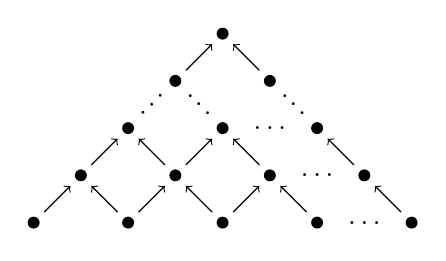
\begin{tikzpicture}[x=0.6cm,y=0.6cm,line cap=round]
		\fill (0,0) circle (0.5ex) coordinate (00);
		\fill (2,0) circle (0.5ex) coordinate (01);
		\fill (4,0) circle (0.5ex) coordinate (02);
		\fill (6,0) circle (0.5ex) coordinate (03);
		\fill (8,0) circle (0.5ex) coordinate (04);
		\fill (1,1) circle (0.5ex) coordinate (10);
		\fill (3,1) circle (0.5ex) coordinate (11);
		\fill (5,1) circle (0.5ex) coordinate (12);
		\fill (7,1) circle (0.5ex) coordinate (13);
		\fill (2,2) circle (0.5ex) coordinate (20);
		\fill (4,2) circle (0.5ex) coordinate (21);
		\fill (6,2) circle (0.5ex) coordinate (22);
		\fill (3,3) circle (0.5ex) coordinate (30);
		\fill (5,3) circle (0.5ex) coordinate (31);
		\fill (4,4) circle (0.5ex) coordinate (40);
		\draw[-to,shorten <=1.25ex,shorten >=1.25ex] (00) -- (10);
		\draw[-to,shorten <=1.25ex,shorten >=1.25ex] (01) -- (10);
		\draw[-to,shorten <=1.25ex,shorten >=1.25ex] (01) -- (11);
		\draw[-to,shorten <=1.25ex,shorten >=1.25ex] (02) -- (11);
		\draw[-to,shorten <=1.25ex,shorten >=1.25ex] (02) -- (12);
		\draw[-to,shorten <=1.25ex,shorten >=1.25ex] (03) -- (12);
		\draw[-to,shorten <=1.25ex,shorten >=1.25ex] (04) -- (13);
		\draw[-to,shorten <=1.25ex,shorten >=1.25ex] (10) -- (20);
		\draw[-to,shorten <=1.25ex,shorten >=1.25ex] (11) -- (20);
		\draw[-to,shorten <=1.25ex,shorten >=1.25ex] (11) -- (21);
		\draw[-to,shorten <=1.25ex,shorten >=1.25ex] (13) -- (22);
		\draw[-to,shorten <=1.25ex,shorten >=1.25ex] (12) -- (21);
		\draw[-to,shorten <=1.25ex,shorten >=1.25ex] (30) -- (40);
		\draw[-to,shorten <=1.25ex,shorten >=1.25ex] (31) -- (40);
		\path (03) to  node[pos=0.5] {$\ldots$} (04);
		\path (12) to  node[pos=0.5] {$\ldots$} (13);
		\path (21) to  node[pos=0.5] {$\ldots$} (22);
		\path (31) to  node[pos=0.5,sloped] {$\ldots$} (22);
		\path (20) to  node[pos=0.5,sloped] {$\ldots$} (30);
		\path (21) to  node[pos=0.5,sloped] {$\ldots$} (30);
	\end{tikzpicture}
\end{center}
And voilà, plenty of spans!
 The corresponding picture for $\Ar(\Delta^n)$ is instead the following:
\begin{center}
	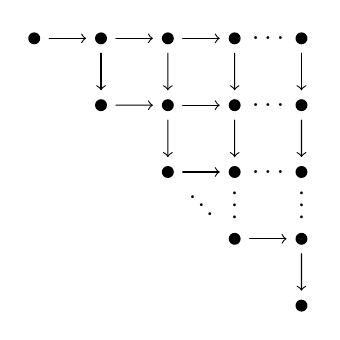
\begin{tikzpicture}[x=0.6cm,y=0.6cm,line cap=round,rotate=-45]
		\fill (0,0) circle (0.5ex) coordinate (00);
		\fill (2,0) circle (0.5ex) coordinate (01);
		\fill (4,0) circle (0.5ex) coordinate (02);
		\fill (6,0) circle (0.5ex) coordinate (03);
		\fill (8,0) circle (0.5ex) coordinate (04);
		\fill (1,1) circle (0.5ex) coordinate (10);
		\fill (3,1) circle (0.5ex) coordinate (11);
		\fill (5,1) circle (0.5ex) coordinate (12);
		\fill (7,1) circle (0.5ex) coordinate (13);
		\fill (2,2) circle (0.5ex) coordinate (20);
		\fill (4,2) circle (0.5ex) coordinate (21);
		\fill (6,2) circle (0.5ex) coordinate (22);
		\fill (3,3) circle (0.5ex) coordinate (30);
		\fill (5,3) circle (0.5ex) coordinate (31);
		\fill (4,4) circle (0.5ex) coordinate (40);
		\draw[-to,shorten <=1.25ex,shorten >=1.25ex] (00) -- (10);
		\draw[-to,shorten <=1.25ex,shorten >=1.25ex] (10) -- (01);
		\draw[-to,shorten <=1.25ex,shorten >=1.25ex] (01) -- (11);
		\draw[-to,shorten <=1.25ex,shorten >=1.25ex] (11) -- (02);
		\draw[-to,shorten <=1.25ex,shorten >=1.25ex] (02) -- (12);
		\path (12) to node[pos=0.5,sloped,rotate=-45] {$\ldots$} (03);
		\draw[-to,shorten <=1.25ex,shorten >=1.25ex] (13) -- (04);
		\draw[-to,shorten <=1.25ex,shorten >=1.25ex] (10) -- (20);
		\draw[-to,shorten <=1.25ex,shorten >=1.25ex] (20) -- (11);
		\draw[-to,shorten <=1.25ex,shorten >=1.25ex] (11) -- (21);
		\draw[-to,shorten <=1.25ex,shorten >=1.25ex] (31) -- (22);
		\draw[-to,shorten <=1.25ex,shorten >=1.25ex] (21) -- (12);
		\path (30) to node[pos=0.5] {$\ldots$} (40);
		\draw[-to,shorten <=1.25ex,shorten >=1.25ex] (40) -- (31);
		\draw[-to,shorten <=1.25ex,shorten >=1.25ex] (20) to  (30);
		\draw[-to,shorten <=1.25ex,shorten >=1.25ex] (03) to  (13);
		\path (02) to  node[pos=0.5,sloped,rotate=-45] {$\ldots$} (03);
		\path (12) to  node[pos=0.5,sloped,rotate=-45] {$\ldots$} (22);
		\path (21) to  node[pos=0.5,sloped,rotate=-45] {$\ldots$} (31);
		\path (22) to  node[pos=0.5,sloped,rotate=-45] {$\ldots$} (13);
		\draw[to-,shorten <=1.25ex,shorten >=1.25ex] (21) to (30);
	\end{tikzpicture}
\end{center}
As a bit of foreshadowing, Fabian mentioned that the first picture is related to the \emph{Quillen $Q$-construction} (see~\cref{par:QuillenQConstruction}), whereas the second is related to the \emph{Segal $S$-construction} (see \cref{con:SConstruction}), which people keep calling \emph{Waldhausen} $S$-construction, even though Waldhausen himself wrote \emph{Segal} $S$-construction.
\begin{exc}\label{exc:coreTwAr=coreAr}
	Show that $\core\TwAr(\Cc)\simeq\core\Ar(\Cc)$ holds for all $\infty$-categories $\Cc$.
\end{exc}
\begin{proof}[Proof sketch]
	See \cite[Proposition~I.31]{KTheory} for a rough sketch.
\end{proof}

\section{Yoneda's Lemma, Limits and Colimits in \texorpdfstring{$\infty$}{Infinity}-Categories}
\subsection{Yoneda's Lemma and Adjunctions}
Now that we have a sufficient supply of mutually equivalent definitions of the $\Hom$ functor, the next step is to prove Yoneda's lemma.
\begin{thm}[Yoneda's lemma]\label{thm:Yoneda}
	Let $\Cc$ be an $\infty$-category. Given a functor $F\colon \Cc\morphism\cat{An}$ and an object $x\in \Cc$, the evaluation map
		\begin{equation*}
			\ev_{\id_x}\colon\Nat\big(\Hom_\Cc(x,-),F\big)\isomorphism F(x)
		\end{equation*}
		is an equivalence \embrace{we use $\Nat$ as a shortcut for $\Hom_{\Fun(\Cc,\cat{An})}$}. Morover, adjoining the functor $\Hom_\Cc\colon\Cc^\op\times\Cc\morphism\Fun(\Cc,\cat{An})$ gives fully faithful functors \embrace{\enquote{Yoneda embeddings}}
		\begin{equation*}
			\Yo^\Cc\colon\Cc\morphism\Fun(\Cc^\op,\cat{An})\quad\text{and}\quad \Yo_\Cc\colon\Cc^\op\morphism\Fun(\Cc,\An)\,.
		\end{equation*}
\end{thm}
%Initially, I used $Y$ to denote the Yoneda embeddings, but then people advised me to use $\Yo$ instead, the hiragana symbol for \emph{yo}, which I think makes a lot of sense.
\begin{proof*}[Proof of \cref{thm:Yoneda}]
	See \cite[Corollaries~XI.2 and~XI.4]{HigherCatsII}.
\end{proof*}
\begin{defi}
	For an $\infty$-category $\Cc$ we denote by $\Pp(\Cc)=\Fun(\Cc^\op,\cat{An})$ the \emph{$\infty$-category of presheaves} on $\Cc$.
\end{defi}
Onwards to adjunctions!
\begin{defi}
	Let $R\colon\Dd\morphism\Cc$ be a functor of $\infty$-categories.
	\begin{alphanumerate}
		\item Given objects $y\in \Cc$, $x\in\Dd$, and a morphism $\eta\colon y\morphism Rx$ in $\Cc$, we say \emph{$\eta$ witnesses $x$ as a left-adjoint object to $y$ under $R$} if the composite
		\begin{equation*}
			\Hom_\Dd(x,-)\morphism[R]\Hom_\Cc(Rx,R-)\morphism[\eta^*]\Hom_\Cc(y,R-) 
		\end{equation*}
		is an equivalence of functors $\Dd\morphism \An$ \embrace{which may be tested on objects by \cref{thm:JoyalEquivalence}\itememph{b}}.
		\item An \emph{adjunction} between $R$ and some functor $L\colon \Cc\morphism\Dd$ is an equivalence
		\begin{equation*}
			\Hom_\Dd(L-,-)\simeq\Hom_\Cc(-,R-)
		\end{equation*}
		as functors $\Cc^\op\times\Cc\morphism\An$.
	\end{alphanumerate}
\end{defi}
A simple but still somewhat surprising and incredibly useful consequence of Yoneda's lemma is that to define left-adjoint functors, it suffices to do so on objects (something that is wildly false for arbitrary functors)!
\begin{cor}\label{cor:AdjointsPointwise}
	A functor $R\colon \Dd\morphism\Cc$ of $\infty$-categories admits a left adjoint if and only if every $y\in \Cc$ admits a left-adjoint object under $R$. More generally, if $\Cc_R\subseteq \Cc$ is the full subcategory spanned by those objects $y\in\Cc$ which admit a left-adjoint object, extracting these left-adjoint objects defines a functor
	\begin{equation*}
		L\colon \Cc_R\morphism \Dd\,.
	\end{equation*}
\end{cor}
\begin{proof}
	We repeat the proof given in \cite[Lemma~XI.6]{HigherCatsII}. Via currying, the functor $\Hom_\Cc(-,R-)\colon \Cc^\op\times\Dd\morphism\cat{An}$ corresponds to a functor $H\colon \Cc^\op\morphism\Fun(\Dd,\cat{An})$. When restricted to $\Cc_R^\op$, it lands in the representables, i.e., in the essential image of the Yoneda embedding $\Yo_\Dd\colon \Dd^\op\morphism\Fun(\Dd,\cat{An})$. By \cref{thm:Yoneda}, $\Yo_\Dd$ is fully faithful, hence an equivalence onto its essential image by \cref{thm:JoyalEquivalence}\itememph{a}. Composing $H|_{\Cc_R^\op}$ with an inverse of this equivalence gives a functor $\Cc_R^\op\morphism\Dd^\op$. Taking $(-)^\op$ we get $L\colon \Cc_R\morphism\Dd$ as required.
	
	By construction, $\Yo_\Dd\circ L^\op$ is equivalent to $H|_{\Cc_R^\op}$ in $\Fun(\Cc_R^\op,\Fun(\Dd,\An))$. But this means that $\Hom_\Dd(L-,-)$ and $\Hom_\Cc(-,R-)$ are equivalent in $\Fun(\Cc_R^\op\times\Dd,\An)$. If $\Cc_R=\Cc$, this proves that $L$ is indeed a left adjoint of $R$.
\end{proof}
\begin{exm}\label{exm:MyFirstAdjoints}
	\enquote{My first adjoint pairs of functors}:
	\begin{alphanumerate}
		\item The inclusion $\cat{An}\subseteq \cat{Cat}_\infty$ has both a left adjoint, the functor $|\blank|\colon \cat{Cat}_\infty\morphism\cat{An}$ (which sends an $\infty$-category to its localisation at all its morphisms), and a right adjoint, given by $\core\colon \cat{Cat}_\infty\morphism\cat{An}$. We proved this in \cite[Example~XI.8]{HigherCatsII}. Moreover, the inclusion $\cat{Set}\morphism\cat{An}$ has $\pi_0\colon\cat{An}\morphism\cat{Set}$ as a left adjoint. In pictures,
		\begin{equation*}
			\begin{tikzcd}
				\Set\rar[symbol=\subseteq] & \An\rar[symbol=\subseteq]\lar[dashed,bend right=45,"\pi_0"']  & \Cat_\infty\lar[dashed,bend right=45,"|\blank|"']\lar[dashed,bend left=45,"\core",shorten >=0.75ex]
			\end{tikzcd}
		\end{equation*}
		Of course we should actually write $\N(\Set)$ instead of $\Set$, but from now on we'll frequently abuse notation that way since writing $\N$ all the time will inevitably get on our \dotso \emph{nerves} (sorry).
		\item Let $\Ii$ be any simplicial set (which we think of as a \enquote{diagram shape}) and consider the functor $\const\colon\Cc\morphism\Fun(\Ii,\Cc)$. Given a map $F\colon \Ii\morphism\Cc$, a left-adjoint object to $F$ under $\const$ is called a \emph{colimit} of $F$ and denoted $\colimit_IF$. Similarly, a right-adjoint object is called a \emph{limit} and denoted $\limit_IF$. In particular, one has
		\begin{equation*}
			\Hom_\Cc\left(\colimit_\Ii F,x\right)\simeq\Nat(F,\const x)
		\end{equation*}
		for all objects $x\in \Cc$, and similarly for $\lim_IF$. We will discuss limits and colimits in detail in the next subsection.
	\end{alphanumerate}
\end{exm}
\subsection{First Properties and Examples of (Co)Limits}
First we'll discuss the main existence theorem for limits and colimits in $\infty$-categories. For that matter, recall the notion of \emph{Kan simplicial model categories} from \cite[Digression~IV Definition~G.2]{HigherCatsII}. For a (not necessarily Kan simplicial) model category $A$, we denote by $A^\mathrm{cf}$ its full subcategory of bifibrant objects (Lurie uses the notation $A^\circ$ instead). Also $(-)^\mathrm{c}\colon A\morphism A$ and $(-)^\mathrm{f}\colon A\morphism A$ denote any choice of cofibrant/fibrant replacement functors.
\begin{thm}\label{thm:HomotopyLimits}
	If $A$ is a Kan simplicial model category, then $\N^c(A^\mathrm{cf})$ has all limits and colimits. For a diagram $F\colon \Ii\morphism \N^c(A^\mathrm{cf})$, these are given by
	\begin{equation*}
		\colimit_\Ii F\simeq \Big(\hocolimit_{\CC[\Ii ]}\snake{F}\Big)^\mathrm{f}\quad\text{and}\quad\limit_\Ii F\simeq\Big(\holimit_{\CC[\Ii]}\snake{F}\Big)^\mathrm{c}\,,
	\end{equation*}
	where $\snake{F}\colon \CC[\Ii]\morphism A^\mathrm{cf}$ is adjoint to $F\colon \Ii\morphism\N^c(A^\mathrm{cf})$.
\end{thm}
\begin{proof*}
	See \cite[Theorem~XI.21]{HigherCatsII}.
\end{proof*}
\begin{rem*}
We'll soon talk about cofinal and final maps (see \cref{def:cofinal} or \cite[\S4.1]{HTT}), but let me already mention that the theory of these allows us to assume that all diagram shapes $\Ii$ are $\infty$-categories. This hardly ever matters, but we formulated \cref{thm:StraighteningCat} for $\infty$-categories only, so I sleep better knowing that $\Ii$ can be chosen that way.
\end{rem*}
\begin{exm}
	Applying \cref{thm:HomotopyLimits} to $A=\sSet$ with its Kan--Quillen model structure or $A=\sSet^+$ (the category of marked simplicial sets) with its marked Joyal model structure, which are Kan simplicial model categories by \cite[Digression~IV Examples~G.3]{HigherCatsII}, shows that $\An$ and $\Cat_\infty$ are complete and cocomplete (i.e.\ have all limits and colimits).
	
	Another example of a complete and cocomplete $\infty$-category is $\Kk(R)$ for any ring $R$, as defined in \cref{exm:MyFirstInftyCats}\itememph{e}. In this case though, we can't apply \cref{thm:HomotopyLimits}, since $\Kk(R)$ is (probably) not given by a Kan simplicial model structure on $\Ch(R)$, at least not for the projective or injective model structure (these have quasi-isomorphisms as weak equivalences, whereas $\Kk(R)$ wants homotopy equivalences). Instead, one has to use some more properties of limits and colimits, which we will develop until \cref{exc:K(R)cocomplete}.
\end{exm}
\begin{exm*}\label{exm*:HomotopyPullbacks}
	Per Bastiaan's suggestion, we give two more examples. Recall that a pullback on the nose in a model category is also a homotopy pullback if all objects are fibrant and one of its legs is a fibration (this follows from Reedy's lemma for example, see \cite[Corollary~VIII.52]{HigherCatsII}). 
	\begin{alphanumerate}
		\item Combining this observation with \cref{thm:HomotopyLimits} shows that the pullback defining $\Hom_\Cc(a,b)$ from \cref{def:Hom} is also a pullback in $\Cat_\infty$, because its vertical leg $\Fun(\Delta^1,\Cc)\morphism\Fun(\partial\Delta^1,\Cc)\simeq \Cc\times\Cc$ is an isofibration (by \cite[Corollary~VII.11]{HigherCatsI}), hence a fibration in the Joyal model structure on $\sSet$.
		\item Likewise, the pullback defining $\Un(F)$ in \cref{thm:StraighteningAn} is a pullback in $\Cat_\infty$, because $*/\An\morphism\An$ is a left fibration, hence an isofibration.
	\end{alphanumerate}
\end{exm*}
For a cocartesian fibration $p\colon E\morphism S$, we denote by $\Gamma(p)$ its \emph{$\infty$-category of sections} defined by the pullback
\begin{equation*}
	\begin{tikzcd}
		\Gamma(p)\rar\dar\drar[pullback] & \Fun(S,E)\dar["p_*"]\\
		\{\id_S\}\rar& \Fun(S,S)
	\end{tikzcd}
\end{equation*}
If we use the new notion from \cref{def:WeirdCocartesianDefinition}\itememph{b} and $p$ is not necessarily an isofibration, we need to take this pullback in $\Cat_\infty$, otherwise it can also be taken in $\sSet$ by the arguments from \cref{exm*:HomotopyPullbacks} above. We let $\Gamma_\cocart(p)\subseteq \Gamma(p)$ denote the full sub-$\infty$-category spanned by sections that take all edges in $S$ to $p$-cocartesian edges.
\begin{prop}[Lurie]\label{prop:CoLimitsInCat}
	Given a diagram $F\colon \Ii\morphism\cat{Cat}_\infty$, we have
	\begin{align*}
		\colimit_\Ii F&\simeq \Un^\cocart(F)\left[\{\text{\upshape cocartesian edges}\}^{-1}\right]\,,\\
		\limit_\Ii F&\simeq \Gamma_\cocart\big(\Un^\cocart(F)\big)\,.
	\end{align*}
	In particular, if $F\colon \Ii\morphism\cat{An}$ takes values in anima, then
	\begin{equation*}
		\colimit_\Ii F\simeq\big|\Un(F)\big|\quad\text{and}\quad\limit_\Ii F\simeq\Gamma\big(\Un(F)\big)\,.
	\end{equation*}
\end{prop}
\begin{proof}[Proof sketch]
	In \cite[Theorem~XI.23]{HigherCatsII} Fabian gave a proof that's basically the same as what we are going to do now, but more on the model category side (but also less sketchy). We only do the case of limits. Consider the diagram
	\begin{equation*}
		\begin{tikzcd}[row sep=small]
			& \Fun(\Ii,\Cat_\infty)\ar[<-,dd,iso,"\St"']\\
			\Cat_\infty\urar["\const",sloped]\drar& \\
			& \Cocart(\Ii)
		\end{tikzcd}
	\end{equation*}
	in which the bottom arrow sends $\Cc\in\Cat_\infty$ to the cocartesian fibration $\pr_2\colon \Cc\times \Ii\morphism \Ii$ over $\Ii$. Let $p\colon E\morphism \Ii$ denote the cocartesian unstraightening of $F$. If $X\simeq\limit_\Ii F$, then we must have equivalences $\Nat(\const\Cc,F)\simeq \Hom_{\Cat_\infty}(\Cc,X)$ for all $\infty$-categories $\Cc$. Applying \cref{thm:StraighteningCat}, this translates into
	\begin{equation*}
		\Hom_{\Cocart(\Ii)}\big((\pr_2\colon \Cc\times \Ii\rightarrow \Ii),(p\colon E\rightarrow \Ii)\big)\simeq \Hom_{\Cat_\infty}(\Cc,X)\,,
	\end{equation*}
	which we'll prove now is fulfilled for $X\simeq\Gamma_\cocart(p)$ (or rather we give an idea why it holds). A map $\phi\colon \Cc\times \Ii\morphism E$ corresponds to a map $\roof{\phi}\colon \Cc\morphism\Fun(\Ii,E)$ via currying. By inspection, $\phi$ commutes with the projection down to $\Ii$ iff $\roof{\phi}$ factors over $\Gamma(p)\morphism E$. Since $\pr_2$-cocartesian edges are precisely those of the form $(\text{equivalence in }\Cc,\text{arbitrary morphism in }\Ii)$, we see that $\phi$ preserves cocartesian edges iff $\roof{\phi}$ sends equivalences $f\colon c\morphism c'$ in $\Cc$ to natural transformations $\eta\colon \roof{\phi}(c)\Rightarrow\roof{\phi}(c')\in\Fun(\Ii,E)_1$ such that for all edges $g\colon i\morphism i'$ in $\Ii$ the composition (or some choice of it)
	\begin{equation*}
		\roof{\phi}(c)(i)\morphism[\eta_i]\roof{\phi}(c')(i)\morphism[g_*]\roof{\phi}(c')(i')
	\end{equation*}
	is $p$-cocartesian in $E$. Since $f\colon c\morphism c'$ is an equivalence in $\Cc$, we get that $\eta_i$ is an equivalence in the fibre $E\times_\Ii\{i\}$ (even in $E$), hence automatically $p$-cocartesian by \cite[Corollary~IX.8]{HigherCatsII}. Thus the composition is $p$-cocartesian iff $g_*$ is $p$-cocartesian, in other words, if $\roof{\phi}(c')$ sends all morphisms in $\Ii$ to $p$-cocartesian edges. Since this holds for all $c'\in \Cc$ (we can always take $f=\id_{c'}$), we finally obtain that $\phi$ preserves $\pr_2$-cocartesian edges iff $\roof{\phi}\colon \Cc\morphism\Gamma(p)$ factors over $\Gamma_\cocart(p)$. \enquote{Thus} $X\simeq \Gamma_\cocart(p)$. 
	
	So far, this is no proof at all, since we only explained why $0$-simplices of $\Nat(\const \Cc,F)$ correspond to $0$-simplices of $\Hom_{\Cat_\infty}(\Cc,\Gamma_\cocart(p))$ but it's not clear how to proceed for higher simplices, nor how to make this an $\infty$-natural transformation. To fix this, first note that we have a map of cocartesian fibrations
	\begin{equation*}
		\begin{tikzcd}
			\Gamma_\cocart(p)\times \Ii\dar["\pr_2"']\rar& E\dar["p"]\\
			\Ii\eqar[r]&\Ii
		\end{tikzcd}
	\end{equation*}
	induced by the evaluation map $\Fun(\Ii,E)\times \Ii\morphism E$. After straightening, this gives a natural transformation $\eta\colon \const\Gamma_\cocart(p)\Rightarrow F$, hence we get
	\begin{equation*}
		\Hom_{\Cat_\infty}\big(-,\Gamma_\cocart(p)\big)\xRightarrow{\const *}\Nat\big(\const-,\const\Gamma_\cocart(p)\big)\overset{\eta_*}{\Longrightarrow}\Nat(\const-,F)\,,
	\end{equation*}
	which is the desired natural transformation. Whether this is an equivalence can be checked pointwise. Since instead of $\Nat(\const-,F)$ we can take the corresponding $\Hom$ anima in $\Cocart(\Ii)$, we arrive at the equivalence from the beginning of the proof. Since we know how to compute $\Hom$ spaces in $\Cat_\infty$ and in $\Cat_\infty/\Ii$ (the latter by \cite[Corollary~VIII.6]{HigherCatsII}), one easily checks $\Hom_{\Cat_\infty}(\Cc,\Gamma(p))\simeq\Hom_{\Cat_\infty/\Ii}((\pr_2\colon\Cc\times \Ii\morphism \Ii),(p\colon E\morphism \Ii))$. Now the $\Hom$ anima we are interested in are full subanima of these, so it really suffices to check that their $0$-simplices correspond, which we did above.
\end{proof}
\begin{exm}\lecture[Localisations. More properties of (co)limits. Left Kan extensions for presheaf categories. $\Hom$ anima in functor categories.]{2020-11-10}\label{exm:Localisation}
	Since $\core\colon\Cat_\infty\morphism\An$ is right-adjoint to the inclusion $\An\subseteq\Cat_\infty$ (\cref{exm:MyFirstAdjoints}\itememph{a}), we get a natural counit transformation $\core\Rightarrow\id_{\Cat_\infty}$, which is given by a map $\Delta^1\morphism\Fun(\Cat_\infty,\Cat_\infty)$. By currying, this yields a functor
	\begin{align*}
		\Cat_\infty&\morphism\Ar(\Cat_\infty)\\
		\Cc&\longmapsto(\core\Cc\rightarrow\Cc)\,.
	\end{align*}
	If $F\colon W\morphism\Cc$ is an object in $\Ar(\Cat_\infty)$, a left-adjoint object to $F$ under the above functor is called a \emph{localisation} of $\Cc$ at $F$ (or rather at the image of $\pi_0\core\Ar(W)\morphism\pi_0\core\Ar(\Cc)$) of $F$ and denoted $\Cc[W^{-1}]$. Unwinding, this means that
	\begin{equation*}
		\Hom_{\Cat_\infty}\big(\Cc[W^{-1}],\Dd\big)\subseteq \Hom_{\Cat_\infty}(\Cc,\Dd)
	\end{equation*}
	is a collection of path components, given by those $G\colon \Cc\morphism\Dd$ such that the composite $G\circ F\colon W\morphism\Dd$ lands in $\core \Dd$. The localisation $\Cc[W^{-1}]$ always exists, as one can take
	\begin{equation*}
		\begin{tikzcd}
			W\rar["F"]\dar\drar[pushout] & \Cc\dar["p"]\\
			{|W|}\rar& \Cc[W^{-1}]
		\end{tikzcd}
	\end{equation*}
	(the pushout is taken in $\Cat_\infty$ of course). Futhermore, it turns out that
	\begin{equation*}
		p^*\colon \Fun\big(\Cc[W^{-1}],\Dd\big)\morphism\Fun(\Cc,\Dd)
	\end{equation*}
	is fully faithful, with essential image spanned by the same functors $G\colon \Cc\morphism\Dd$ as above (see \cite[Proposition~VIII.7]{HigherCatsII} for a proof). This has the funny consequence that the Yoneda embedding induces fully faithful inclusions $\Cc[W^{-1}]\subseteq \Pp\big(\Cc[W^{-1}]\big)\subseteq \Pp(\Cc)$.
	In other words, all localisations of $\Cc$ occur as full subcategories of $\Pp(\Cc)$, which puts a size bound on how large $\Cc[W^{-1}]$ can be.
\end{exm}
\numpar*{Warning \smash{\Attention}}
Localisations are difficult! Localisations of locally small $\infty$-categories may not be locally small any more. Moreover, the localisation of a $1$-category may not be a $1$-category any more.
\begin{exm}\label{exm:Delta0Pushout}
	Let's compute the pushout
	\begin{equation*}
		\begin{tikzcd}
			\Delta^0\rar["1"]\drar[pushout]\dar["0"']& \Delta^1\dar[dashed]\\
			\Delta^1\rar[dashed]& \boldsymbol{?}
		\end{tikzcd}
	\end{equation*}
	in $\Cat_\infty$. One way to do this would be to notice that $0\colon \Delta^0\morphism\Delta^1$ is a cofibration in the Joyal model structure on $\sSet$ (and so is $1\colon \Delta^0\morphism\Delta^1$, but we don't even need this) and all objects are cofibrant, hence the pushout on the nose, which is the $2$-spine $I^2$, is also a homotopy pushout. Now $I^2\subseteq\Delta^2$ is inner anodyne, hence $\Delta^2$ is a fibrant replacement of $I^2$ in the Joyal model structure, which shows that $\boldsymbol{?}\simeq \Delta^2$ is really the pushout in question by \cref{thm:HomotopyLimits}.
	
	 For educational purposes, Fabian presented a less efficient way to show $\boldsymbol{?}\simeq \Delta^2$ using \cref{prop:CoLimitsInCat}. Consider the pushout diagram above as a map $F\colon\Lambda_0^2\morphism\Cat_\infty$. Since all maps in the diagram are nerves of functors of $1$-categories, the cocartesian unstraightening $\Dd=\Un^\cocart(F)$ is simply given by the Grothendieck construction. Therefore, the cocartesian fibration $\Dd\morphism \Lambda_0^2$ can be pictured as follows:
	\begin{center}
		\begin{tikzpicture}[x=0.6cm,y=0.6cm,line cap=round, line join=round]
			\fill (0,0) circle (0.5ex) coordinate (A);
			\fill (-2,0) circle (0.5ex) coordinate (B);
			\fill (-2,1.5) circle (0.5ex) coordinate (C);
			\fill (2,0) circle (0.5ex) coordinate (D);
			\fill (2,1.5) circle (0.5ex) coordinate (E);
			\fill (0,-2.5) circle (0.5ex) coordinate (F);
			\fill (-2,-2.5) circle (0.5ex) coordinate (G);
			\fill (2,-2.5) circle (0.5ex) coordinate (H);
			\node at (-1.4,0.45) {$\scriptscriptstyle /\!/\!/$};
			\draw[dotted, rounded corners=2] (-1.2cm-1ex,0.9cm-1ex) -- (-1ex,-1ex) -- (1.2cm+1ex,-1ex) -- (1.2cm+1ex,0.9cm+1ex) -- (-1.2cm-1ex,0.9cm+1ex) -- cycle;
			\draw[-to,shorten <=1.25ex,shorten >=1.25ex,FabiansPink] (A) to (B);
			\draw[-to,shorten <=1.25ex,shorten >=1.25ex,FabiansPurple!67!FabiansPink] (B) to (C);
			\draw[-to,shorten <=1.25ex,shorten >=1.25ex] (A) to (C);
			\draw[-to,shorten <=1.25ex,shorten >=1.25ex,FabiansPink] (A) to (E);
			\draw[-to,shorten <=1.25ex,shorten >=1.25ex] (D) to (E);
			\draw[-to,shorten <=1.25ex,shorten >=1.25ex] (F) to (G);
			\draw[-to,shorten <=1.25ex,shorten >=1.25ex] (F) to (H);
			\draw[|-to] (0,-0.75cm+0.5\morphismlength) to ++(0,-\the\morphismlength);
			\node at (-3,-2.5) {$\Lambda_0^2$};
			\node at (-3,0.75) {$\Dd$};
			\node at (3,0.75) {$\Dd'$};
		\end{tikzpicture}
	\end{center}
	The two pink edges are the cocartesian ones and thus sent to equivalences in the localisation $\Dd[\{\text{cocartesian edges}\}^{-1}]=\Dd[\{\text{pink edges}\}^{-1}]$. Let $\Dd'$ be the $\infty$-category obtained from $\Dd$ by removing the purple and the pink edge on the left, together with the $2$-simplex spanned by them. We claim that the restriction
	\begin{equation*}
		\Fun^{\{\text{pink}\}}(\Dd,\Ee)\isomorphism \Fun^{\{\text{pink}\}}(\Dd',\Ee)
	\end{equation*}
	is an equivalence for any $\infty$-category $\Ee$, where $\Fun^{\{\text{pink}\}}$ denotes functors that send pink edges to equivalences. Indeed, the purple edge on the left is \enquote{superfluous data}, i.e., any map $\Dd\smallsetminus\{\text{purple edge}\}\morphism\Ee$ has a contractible space of lifts to $\Dd$, by Joyal's lifting theorem. Moreover any map $\Dd'\morphism\Ee$ has a contractible space of lifts to a map $\Dd\smallsetminus\{\text{purple edge}\}\morphism\Ee$ that sends the left pink edge to an equivalence. This proves the above equivalence.
	
	A similar argument shows that it doesn't matter whether we send the pink edge on the right to an equivalence or to an actual identity in $\Ee$. Thus
	\begin{equation*}
		\Fun^{\{\text{pink}\}}(\Dd',\Ee)\simeq\Fun(\Lambda_1^2,\Ee)\simeq\Fun(\Delta^2,\Ee)\,,
	\end{equation*}
	which proves that $\Dd[\{\text{cocartesian edges}\}^{-1}]\simeq\Delta^2$, as claimed.
\end{exm}
\begin{lem}\label{lem:f^*preservesColimits}
	If $\Cc$ is complete or cocomplete, then so is $\Fun(\Dd,\Cc)$ for any $\Dd$. Furthermore, for any $f\colon \Ee\morphism\Dd$, the precomposition functor
	\begin{equation*}
		f^*\colon \Fun(\Dd,\Cc)\morphism\Fun(\Ee,\Cc)
	\end{equation*}
	preserves limits and colimits. In particular \embrace{taking $f$ to be $\{d\}\monomorphism\Dd$ for any $d\in \Dd$}, limits and colimits in functor categories are computed pointwise.
\end{lem}
For the proof we need the following observation.
\begin{obs}\label{obs:AdjunctionOfFunctorCats}
	If $L\colon \Cc \shortdoublelrmorphism \Dd\noloc R$ are adjoint functors, then so are
	\begin{equation*}
		L_*\colon\Fun(\Ee,\Cc)\doublelrmorphism \Fun(\Ee,\Dd)\noloc R_*\quad\text{and}\quad
		R^*\colon\Fun(\Dd,\Ee)\doublelrmorphism \Fun(\Cc,\Ee)\noloc L^*
	\end{equation*}
for any $\infty$-category $\Ee$.
\end{obs}
\begin{proof}
	Being adjoints can be characterized by the existence of a unit and a counit transformation satisfying the triangle identities (see \cite[Proposition~XI.14]{HigherCatsII}, and $L_*$, $R_*$ inherit these transformations from $L$, $R$. Same for $R^*$, $L^*$.
\end{proof}
\begin{obs}\label{obs:AdjointsPreserveLimits}
	Left-adjoint functors preserve colimits, right-adjoint functors preserve limits.
\end{obs}
\begin{proof}
	Straightforward calculation using \cref{obs:AdjunctionOfFunctorCats}. See \cite[Lemma~XI.22]{HigherCatsII} for details.
\end{proof}
\begin{proof}[Proof of \cref{lem:f^*preservesColimits}]
	For any diagram shape $\Ii$, consider the commutative diagram
	\begin{equation*}
		\begin{tikzcd}[row sep=small]
			& \Fun\big(\Ii,\Fun(\Dd,\Cc)\big)\eqar[dd]\\
			\Fun(\Dd,\Cc)\urar["\const",sloped]\drar["\const *"', sloped]& \\
			& \Fun\big(\Dd,\Fun(\Ii,\Cc)\big)\ular[dotted, bend right,"\colimit_*"', end anchor=east,start anchor=160,shorten <=2ex]\ular[dotted, bend left,"\limit_*",start anchor=west, end anchor=330]
		\end{tikzcd}
	\end{equation*}
	By \cref{obs:AdjunctionOfFunctorCats}, $\colimit_*$ and $\limit_*$ are left and right adjoints of $\const *$ respectively, which proves that $\const\colon \Fun(\Dd,\Cc)\morphism \Fun(\Ii,\Fun(\Dd,\Cc))$ has a left and right adjoint as well. Hence $\Fun(\Dd,\Cc)$ is complete and cocomplete again. Moreover, the assertion that limits and colimits are computed pointwise follows by unraveling.
	
	It remains to show that $f^*\colon \Fun(\Dd,\Cc)\morphism\Fun(\Ee,\Cc)$ preserves limits and colimits. For any diagram $F\colon \Ii\morphism\Fun(\Dd,\Cc)$ we get a map
	\begin{equation*}
		\colimit_\Ii f^*F\morphism f^*\colimit_\Ii F
	\end{equation*}
	(unique up to contractible choice). Whether this is an equivalence in $\Fun(\Ee,\Cc)$ can be checked pointwise (by \cref{thm:JoyalEquivalence}\itememph{b}), i.e., after composition with $x^*\colon \Fun(\Ee,\Cc)\morphism\Fun(\{x\},\Cc)\simeq \Cc$ for all $x\in \Ee$. Since we already know that colimits in $\Fun(\Ee,\Cc)$ and $\Fun(\Dd,\Cc)$ are computed pointwise, we see that both $x^*\colimit_\Ii f^*F$ and $x^*f^*\colimit_\Ii F$ are colimits of the diagram $\Ii\times\{f(x)\}\morphism \Cc$ induced by currying of $F$ and restriction along $\{f(x)\}\monomorphism\Dd$.
\end{proof}
\begin{prop}\label{prop:ColimitsCommute}
	Let $p\colon \Ee\morphism\Cc$ be a cocartesian fibration and $F\colon \Ee\morphism\Dd$ a diagram. Suppose that the restrictions $F_{|c}\colon\Ee_{|c}\morphism\Dd$ of $F$ to the fibres $\Ee_{|c}=\Ee\times_\Cc\{c\}$ of $p$ have colimits for all $c\in \Cc$. Then these assemble into a functor $G\colon \Cc\morphism\Dd$ sending $c\mapsto \colimit_{\Ee_{|c}}F_{|c}$, and
	\begin{equation*}
		\colimit_\Ee F\simeq \colimit_\Cc G\,,
	\end{equation*}
	whenever either exists. In particular \embrace{taking $p$ to be the projection $\pr_2\colon \Ii\times\Cc\morphism\Cc$ for some $\infty$-category $\Ii$}, this means that \enquote{colimits commute}. Also a dual assertion holds, with $p$ a cartesian fibration and all colimits replaced by limits.
\end{prop}
\begin{proof*}
	Fabian claims (I think) this follows from \cite[Proposition~\HTTthm{4.3.2.12}]{HTT}, but Lurie's proof is rather laborious, so I'll give my own proof*. As it turns out, the arguments are pretty much the same as for the proof of Theorems~\labelcref{thm:ColimitPreservingRepresentable,thm:KanExtension} in Fabians notes. I'll freely reference later results (without running into circular arguments, I hope).
	
	We won't prove the assertion as stated above, but its dualized version. The reason is that the direct proof of the undualized version is quite confusing (for example, neither of the Yoneda embeddings preserves colimits, so we would have to consider $(\Yo^\Dd)^\op\colon \Dd^\op\morphism\Pp(\Dd)^\op$) and it seems cleaner to prove the dualized statement and then deduce the undualized one by applying the dual statement to $p^\op\colon \Ee^\op\morphism\Cc^\op$.
	
	So let $p\colon \Ee\morphism\Cc$ be cartesian instead. We want to construct $G$ as the right Kan extension $G\simeq p_*F$. Let's first consider the case where $\Dd$ is replaced by $\Pp(\Dd)$. Then the dual of \cref{thm:StraighteningAn} implies $\Fun(\Cc,\Pp(\Dd))\simeq \Fun(\Cc\times\Dd^\op,\An)\simeq \Right(\Cc^\op\times\Dd)$ and same for $\Ee$, so we may apply \cref{lem*:SmoothBaseChange} below to the cocartesian fibration $p^\op\times\id_\Dd\colon \Ee^\op\times\Dd\morphism\Cc^\op\times\Dd$ to see that $p^*\colon \Fun(\Cc,\Pp(\Dd))\morphism\Fun(\Ee,\Pp(\Dd))$ has a right adjoint $p_*$. Now consider the diagram
	\begin{equation*}
		\begin{tikzcd}
			\Fun\big(\Cc,\Pp(\Dd)\big)\rar["p^*"]\dar["c^*"']& \Fun\big(\Ee,\Pp(\Dd)\big)\dar["i^*"]\\
			\Fun\big(\{c\},\Pp(\Dd)\big)\rar["p_{|c}^*"]& \Fun\big(\Ee_{|c},\Pp(\Dd)\big)
		\end{tikzcd}
	\end{equation*}
	where $i\colon \Ee_{|c}\monomorphism \Ee$ denotes the inclusion of the fibre. The second part of \cref{lem*:SmoothBaseChange} ensures that $c^*p_*F\simeq p_{|c,*}i^*F$. By inspection, right Kan extension along the functor $p_{|c}\colon \Ee_{|c}\morphism\{c\}$ is given by taking a functor $G\colon \Ee_{|c}\morphism\Pp(\Dd)$ to $\limit_{\Ee_{|c}}G$. This implies $p_*F(c)\simeq \limit_{\Ee_{|c}}F_{|c}$, so $p_*F$ takes the correct values. Moreover, limits over $\Cc$ are given by right Kan extension along the unique map $\pi\colon \Cc\morphism *$, and similar for $\pi\circ p\colon \Ee\morphism *$, hence
	\begin{equation*}
		\limit_\Cc p_*F\simeq \pi_*p_*F\simeq (\pi\circ p)_*F\simeq \limit_\Ee F
	\end{equation*}
	since right adjoints compose. This finishes the proof for $\Pp(\Dd)$.
	
	Now for the case of general $\Dd$. The Yoneda embedding $\Yo^\Dd\colon \Dd\morphism\Pp(\Dd)$ is fully faithful, hence an equivalence onto its essential image. To obtain a functor $p_*F\colon \Cc\morphism\Dd$, it thus suffices to check that $p_*(\Yo^\Dd\circ F)\colon \Cc\morphism\Pp(\Dd)$ has image in the representable functors. By assumption, all limits $\limit_{\Ee_{|c}}F_{|c}$ exist in $\Dd$ and $\Yo^\Dd$ preserves limits by \cref{cor:HomPreservesColimits}, hence the description of the values $p_*(Y\circ F)(c)$ for $c\in \Cc$ shows that indeed it takes values in the representables. Thus $p_*F\colon \Cc\morphism\Dd$ exists. The additional assertion about limits follows as above, noting that the limits in question exist in $\Dd$ if and only if the limits taken in $\Pp(\Dd)$ (where they definitely exist) are representable, since $\Yo^\Dd$ is fully faithful and preserves limits.
\end{proof*}
\begin{lem*}\label{lem*:SmoothBaseChange}
	Let $p\colon \Cc\morphism\Dd$ be a cocartesian fibration of $\infty$-categories. Consider a pullback square \embrace{inside $\Cat_\infty$} as on the left
	\begin{equation*}
		\begin{tikzcd}
			\Cc'\rar["q"]\dar["g"']\drar[pullback] & \Dd'\vphantom{(}\dar["f"]\\
			\Cc\rar["p"]& \Dd \vphantom{(}
		\end{tikzcd}\quad\longrightsquigarrow{\morphismlength-0.145em}\quad\begin{tikzcd}
		\Right(\Cc')\rar[dotted,bend right,"q_*"]& \Right(\Dd')\lar["q^*"']\\
		\Right(\Cc)\uar["g^*"]\rar[dotted,bend right,"p_*"] & \Right(\Dd)\uar["f^*"']\lar["p^*"']
	\end{tikzcd}
	\end{equation*}
	inducing a square as on the right. Then $p^*$ and $q^*$ have right adjoints $p_*$ and $q_*$ as indicated. Moreover, there's a natural equivalence
	\begin{equation*}
		f^*p_*\overset{\sim}{\Longrightarrow} q_*g^*\,.
	\end{equation*}
\end{lem*}
\begin{proof*}
	Without loss of generality all cartesian or right fibrations can be taken in the old sense. Recall (e.g.\ from the dual of \cite[\S2.1.4]{HTT}) that there exists the \emph{contravariant model structure} on $\sSet/\Cc$, in which the cofibrations are monomorphisms of simplicial sets and fibrant objects are given by right fibrations over $\Cc$ (general fibrations are more complicated). The functor $p^*\colon\sSet/\Dd\morphism\sSet/\Cc$ has a right adjoint $p_*$ for abstract reasons: It's straightforward to check that $p^*$ preserves colimits, so \cref{thm:2Yoneda} can be applied to $\sSet/\Dd\simeq\Pp((\Delta/\Dd)^\op)$ (here $\Delta/S$ denotes the slice category with respect to the functor $\Delta\colon \IDelta\morphism\sSet$ sending $[n]\mapsto \Delta^n$). We claim that
	\begin{equation*}
		p^*\colon \sSet/\Dd\doublelrmorphism\sSet/\Cc\noloc p_*
	\end{equation*}
	is even a Quillen adjunction when $p$ is a cocartesian fibration. Indeed, it's clear that $p^*$ preserves cofibrations and cofibrant objects. For preservation of trivial cofibrations, we refer to \cite[Proposition~\HTTthm{4.1.2.15}]{HTT} or the dual of \cite[Proposition~X.43]{HigherCatsII} for the essential case.
	
	As for any Quillen adjunction of model categories, we get an induced adjunction
	\begin{equation*}
		Lp^*\colon (\sSet/\Cc)_\infty\doublelrmorphism(\sSet/\Dd)_\infty\noloc Rp_*
	\end{equation*}
	on underlying $\infty$-categories, defined as the localisations at all weak equivalences, or equivalently as $\N^c((\sSet/\Cc)^{\mathrm{cf}})$ and $\N^c((\sSet/\Cc)^{\mathrm{cf}})$, since $\sSet/\Cc$ and $\sSet/\Dd$ can be made into a Kan simplicial model categories, so \cite[Digression~III Theorem~D]{HigherCatsII} applies. The latter description shows that the underlying $\infty$-categories identify with $\Right(\Cc)$ and $\Right(\Dd)$. Hence $Lp^*$ (which we abbreviate to $p^*$ in the following) has indeed an adjoint $Rp_*$ (which we abbreviate to $p_*$).
	
	So $p_*$ and $q_*$ exist. The counit $p^*p_*\Rightarrow \id$ induces a transformation $q^*f^*p_*\simeq g^*p^*p_*\Rightarrow g^*$, whose adjoint is the transformation $f^*p_*\Rightarrow q_*g^*$. Whether this is an equivalence can be checked on objects. However, explicitly computing $p_*$ and $q_*$ is nasty, so we employ a trick: By Yoneda, it suffices to check that $\Hom_{\Right(\Dd')}(-,f^*p_*-)\Rightarrow \Hom_{\Right(\Dd')}(-,q_*g^*-)$ is a natural equivalence. But $f^*$ and $g^*$ have left adjoints $f_!$ and $g_!$ by \cref{thm:JoyalRightFibrations}, so we may as well show that $\Hom_{\Right(\Cc)}(p^*f_!-,-)\Rightarrow \Hom_{\Right(\Cc)}(g_!q^*-,-)$ is an equivalence, i.e., that $g_!q^*\Rightarrow p^*f_!$ is an equivalence. This is now easily checked on objects: Unravelling, we need to prove that if $X\epimorphism\Dd'$ is a right fibration and $X\monomorphism Y\epimorphism \Dd$ is a factorisation into a right anodyne and a right fibration, then $X\times_\Dd\Cc\monomorphism Y\times_\Dd\Cc$ is right anodyne again, which follows from the references above since $p\colon \Cc\morphism\Dd$ is cocartesian.
\end{proof*}
\begin{thm}[Joyal's version of Quillen's Theorem A]\label{thm:JoyalQuillenThmA}
	For a functor $\alpha\colon \Ii\morphism \Jj$ the following statements are equivalent.
	\begin{alphanumerate}
		\item A functor $F\colon \Jj\morphism\Cc$ has a colimit iff the composition $F\circ\alpha\colon \Ii\morphism \Cc$ has a colimit, and in this case
		\begin{equation*}
			\colimit_\Ii F\circ\alpha\simeq\colimit_\Jj F\,.
		\end{equation*}
		\item For all $j\in \Jj$ we have $|j/\alpha|\simeq *$, i.e., the slice category $j/\alpha$ is weakly contractible. Here we define $j/\alpha$ by the pullback
		\begin{equation*}
			\begin{tikzcd}[column sep=large]
				j/\alpha\dar \rar\drar[pullback]&\Ar(\Jj)\dar["{(s,t)}"]\\
				\{j\}\times\Ii\rar["{(\operatorname{incl},\alpha)}"]&\Jj\times \Jj
			\end{tikzcd}
		\end{equation*}
		Also observe that $j/\alpha=\Ii\times_\Jj j/\Jj$, which is how people usually denote this in the literature.
	\end{alphanumerate}
\end{thm}
\begin{proof*}
	Combine \cite[Proposition~\HTTthm{4.1.1.8}]{HTT} (for more equivalent characterisations) and \cite[Theorem~\HTTthm{4.1.3.1}]{HTT} (for the actual proof).
\end{proof*}
\begin{defi}\label{def:cofinal}
	Maps $\alpha\colon \Ii\morphism \Jj$ as in \cref{thm:JoyalQuillenThmA} are called \emph{cofinal}. Dually, if precomposition with $\alpha$ preserves limits and detects their existence, then $\alpha$ is called \emph{final}.
\end{defi}
Cofinal maps induce homotopy equivalences $|\alpha|\colon |\Ii|\morphism|\Jj|$ of anima, which can be seen via the chain of homotopy equivalences
\begin{equation*}
	|\Ii|\simeq\colimit_\Ii\const *\simeq\colimit_\Jj\const *\simeq|\Jj|
\end{equation*}
(the colimits in the middle are taken in $\An$). Here we use $|\Ii|\simeq\colimit_\Ii\const *$, which can be seen in several ways: One could use \cref{thm:HomotopyLimits} and the Bousfield--Kan formula (\cite[Digression~III]{HigherCatsII}). Alternatively, compute $\Hom_{\An}(\colimit_\Ii\const *,K)\simeq \limit_\Ii\Hom_{\An}(*,K)\simeq\limit_\Ii K$ for any anima $K$ using \cref{cor:HomPreservesColimits} below, and apply \cref{prop:CoLimitsInCat} to get $\limit_\Ii K\simeq\Gamma(\pr_2\colon K\times \Ii\morphism\Ii)$. The space of sections of $\pr_2\colon K\times\Ii\morphism\Ii$ clearly identifies with $\Fun(\Ii,K)\simeq\core\Fun(\Ii,K)\simeq\Hom_{\Cat_\infty}(\Ii,K)$, so $\colimit_\Ii\const *$ is indeed a left-adjoint object of $\Ii$ under the inclusion $\An\subseteq\Cat_\infty$.

Examples of cofinal maps are given by right-adjoint functors and localisations. Indeed, if $\alpha\colon \Ii\morphism\Jj$ is a right adjoint, then consider the diagram
\begin{equation*}
	\begin{tikzcd}[column sep=small]
		& \Cc\dlar["\const"{sloped}]\drar["\const"{sloped}]& \\
		\Fun(\Jj,\Cc)\ar[rr,"\alpha^*"]\urar[bend left=45, dotted,"\colimit_\Jj"] & & \Fun(\Ii,\Cc)\ular[bend right=45, dotted,"\colimit_\Ii"']
	\end{tikzcd}
\end{equation*}
By \cref{obs:AdjunctionOfFunctorCats}, $\alpha^*\colon \Fun(\Jj,\Cc)\morphism\Fun(\Ii,\Cc)$ is a left-adjoint. Since left-adjoints compose, we obtain $\colimit_\Jj\simeq {\colimit_\Ii}\circ\alpha^*$, as required. If $p\colon \Cc\morphism\Cc[W^{-1}]$ is a localisation and $F\colon \Cc[W^{-1}]\morphism\Dd$ is any diagram, then 
\begin{equation*}
	\Nat(F,\const x)\simeq\Nat(F\circ p,\const x)
\end{equation*}
holds for every $x\in \Cc$ since $p^*\colon \Fun(\Cc[W^{-1}],\Dd)\morphism\Fun(\Cc,\Dd)$ is fully faithful, which again proves cofinality by means of \cref{thm:JoyalQuillenThmA}\itememph{a}.
\begin{cor}\label{cor:ColimitsCommute}
	Let $G\colon \Ii\morphism\Cat_\infty$ be a diagram and put $\Jj\simeq\colimit_\Ii G$. Let $F\colon \Jj\morphism\Dd$ be another diagram and suppose that the restrictions 
	\begin{equation*}
		G(i)\morphism\Jj\morphism[F]\Dd
	\end{equation*}
	have colimits for all $i\in \Ii$. Then these colimits assemble into a functor $H\colon \Ii\morphism \Dd$ sending $i\mapsto \colimit_{G(i)}F$, and we have
	\begin{equation*}
		\colimit_\Jj F\simeq\colimit_\Ii H
	\end{equation*}
	if either exists.
\end{cor}
\begin{proof}
	By \cref{prop:CoLimitsInCat}, we have $\Jj\simeq\colimit_\Ii G\simeq \Un^\cocart(G)[\{\text{cocartesian edges}\}^{-1}]$. Since localisations are cofinal, we obtain
	\begin{equation*}
		\colimit_\Jj F\simeq\colimit_{\Un^{\cocart}(G)}F\,.
	\end{equation*}
	Now recall that $G(i)\simeq \Un^\cocart(G)\times_\Ii\{i\}$, so we are done by \cref{prop:ColimitsCommute}.
\end{proof}
\numpar{\enquote{Corollary}}\label{cor:completeIffPullbacksProducts}\itshape If $\Cc$ has coproducts and pushouts, then it is cocomplete. Dually, if $\Cc$ has products and pullbacks, then it is complete.\upshape
\begin{proof}[\enquote{Proof} sketch]
	Decompose any test category $\Ii$ into its skeleta and repeatedly apply \cref{cor:ColimitsCommute} using $\colimit_{\Delta^n}F=F(n)$ since $\{n\}\monomorphism \Delta^n$ is cofinal---in fact, all right anodyne maps are cofinal. For a complete proof, check out \cite[Proposition~\HTTthm{4.4.2.6}]{HTT}.
\end{proof}
\subsection{Colimits and the Yoneda embedding}
We start with an existence result for \enquote{Kan extensions} which was already used in the proof* of \cref{prop:ColimitsCommute}.
\begin{thm}[Joyal]\label{thm:JoyalRightFibrations}
	Given an arbitrary functor $f\colon \Cc\morphism\Dd$ of $\infty$-categories, the pullback functor 
	\begin{equation*}
		f^*\colon \Right(\Dd)\morphism\Right(\Cc)
	\end{equation*}
	admits a left-adjoint. Its value on $p\colon \Ee\morphism\Cc$ is obtained by factoring $\Ee\morphism\Cc\morphism\Dd$ as a cofinal map followed by a right fibration $p'\colon\Ee'\morphism\Dd$. In diagrams
	\begin{equation*}
		\begin{tikzcd}
			\Ee\dar["p"']\rar& \Ee'\dar["\vphantom{p}\smash{p'}"]\\
			\Cc\rar["f"]&\Dd
		\end{tikzcd}
	\end{equation*}
	where the top arrow is cofinal.
\end{thm}
\begin{proof*}[Proof sketch]
	One way to prove this would be to use the contravariant model structures on $\sSet/\Cc$ and $\sSet/\Dd$ as in the proof* of \cref{lem*:SmoothBaseChange}: One shows that $f^*\colon \sSet/\Dd\morphism\sSet/\Cc$ has a left Quillen adjoint $f_!$, sending $\Ee\morphism\Cc$ to $\Ee\morphism\Cc\morphism\Dd$. Since right anodyne maps are cofinal (\cite[Proposition~\HTTthm{4.1.1.3}]{HTT} or \cite[Theorem~XI.28]{HigherCatsII}), a quick unraveling shows that $Lf_!$ can indeed be described as above.
	
	However, Bastiaan has pointed out a simpler proof that doesn't need any model categories. We will proceed in three steps:
	\begin{numerate}\itshape
		\item The pullback functor $f^*\colon \Cat_\infty/\Dd\morphism\Cat_\infty/\Cc$ \embrace{where we take the pullback along $f$ in $\Cat_\infty$} has a left adjoint. On objects, it is the \enquote{forgetful functor} sending $p\colon \Ee\morphism\Cc$ to $f\circ p\colon \Ee\morphism\Cc\morphism\Dd$.
		\item Under the fully faithful inclusions $\Right(\Cc)\subseteq\Cat_\infty/\Cc$ and $\Right(\Dd)\subseteq\Cat_\infty/\Dd$, the pullback functor $f^*\colon \Cat_\infty/\Dd\morphism\Cat_\infty/\Cc$ restricts to $f^*\colon \Right(\Dd)\morphism\Right(\Cc)$ from the formulation of the theorem.
		\item The fully faithful inclusion $\Right(\Dd)\subseteq\Cat_\infty/\Dd$ has a left adjoint, sending an object $q\colon\Ee\morphism\Dd$ to $q'\colon\Ee'\morphism\Dd$, where $\Ee\morphism\Ee'\morphism\Dd$ is any factorisation into a cofinal map followed by a right fibration.
	\end{numerate}
	
	Since left adjoints compose, combining \itememph{1}, \itememph{2}, and \itememph{3} shows that $f^*\colon \Right(\Dd)\morphism\Right(\Cc)$ has a left adjoint $f_!$ with the desired description on objects.
		
	To show \itememph{1}, we use \cref{cor:AdjointsPointwise} to see that it suffices to show that $f\circ p$ is a left adjoint object of $p$ for any $(p\colon \Ee\morphism\Cc)\in \Cat_\infty/\Cc$. If we had the dual of \cref{cor:HomPreservesColimits} below already, this would be almost trivial, but as it is, we need to be a bit careful. Factor $f\circ p$ into a Joyal equivalence $\Ee\morphism \Ee'$ followed by an isofibration $p'\colon\Ee'\morphism\Dd$. Then $f^*\Ee'$ equals the same pullback taken in $\sSet$ by \cref{thm:HomotopyLimits}. Hence there is a natural map $\Ee\morphism f^*\Ee'$. Together with functoriality of $f^*$, it induces natural transformations
	\begin{align*}
		\Hom_{\Cat_\infty/\Dd}(\Ee,-)\simeq \Hom_{\Cat_\infty/\Dd}(\Ee',-)&\Longrightarrow \Hom_{\Cat_\infty/\Cc}\big(f^*\Ee',f^*(-)\big)\\
		&\Longrightarrow \Hom_{\Cat_\infty/\Cc}\big(\Ee,f^*(-)\big)\,.
	\end{align*}
	We are to show that the composite is an equivalence. By \cref{thm:JoyalEquivalence}\itememph{b}, this can be done on objects. Let $T\morphism\Dd$ be an bject of $\Cat_\infty/\Dd$, which we may choose to be an isofibration without restriction, so that $f^*(T)$ agrees with the corresponding pullback in $\sSet$. Consider $\Fun_\Dd(\Ee,T)\coloneqq\Fun(\Ee,T)\times_{\Fun(\Ee,\Dd)}\{f\circ p\}$ and define $\Fun_\Cc(\Ee,f^*(T))$ similarly. Since $T\morphism\Dd$ is an isofibration, it doesn't matter whether this pullback is taken in $\sSet$ or in $\Cat_\infty$. Moreover, $\core(-)$ transforms pullbacks in $\Cat_\infty$ into pullbacks in $\An$ (it is a right adjoint by \cref{exm:MyFirstAdjoints}\itememph{a}, so \cref{obs:AdjointsPreserveLimits} can be applied), hence our computation of $\Hom$ anima in slice categories from \cite[Corollary~VIII.6]{HigherCatsII} shows $\Hom_{\Cat_\infty/\Dd}(\Ee,T)\simeq \core \Fun_\Dd(\Ee,T)$. Likewise, $\Hom_{\Cat_\infty/\Cc}(\Ee,f^*(T))\simeq \core \Fun_\Cc(\Ee,f^*(T))$. Now the universal property of $f^*(T)$ as a pullback in $\sSet$ implies $\Fun_\Dd(\Ee,T)\simeq \Fun_\Cc(\Ee,f^*(T))$, which proves step~\itememph{1}.
	
	For \itememph{2}, observe that $f^*$ of a right fibration in the old sense can also be taken in $\sSet$ by \cref{thm:HomotopyLimits} again, and right fibrations (in the old sense) are preserved under pullbacks formed in $\sSet$. Hence right fibrations in the new sense are preserved by pullbacks in $\Cat_\infty$.
	
	Finally, to show \itememph{3}, we can argue as \itememph{1} to reduce the assertion to $\Fun_\Dd(\Ee',T)\simeq\Fun_\Dd(\Ee,T)$ for any right fibration $T\morphism\Dd$ and any cofinal map $\Ee'\morphism \Ee$ over $\Dd$. 	But this is precisely how Lurie defines cofinal maps in \cite[Definition~\HTTthm{4.1.1.1}]{HTT}, and his definition is equivalent to our \cref{def:cofinal}.
\end{proof*}
\begin{cor}\label{cor:f_!:PC->PD}
	The functor $f^*\colon \Pp(\Dd)\morphism\Pp(\Cc)$ has a left-adjoint $f_!$ \embrace{given by left Kan extension} such that the diagram
	\begin{equation*}
		\begin{tikzcd}
			\Cc\rar["f"]\dar["\Yo^\Cc"']& \Dd\dar["\Yo^\Dd"]\\			\Pp(\Cc)\rar["f_!"]&\Pp(\Dd)
		\end{tikzcd}
	\end{equation*}
	 commutes in the $\infty$-category $\Cat_\infty$.
\end{cor}
\begin{proof}
	The first statement immediately follows from \cref{thm:JoyalRightFibrations} and (the dual of) \cref{thm:StraighteningAn}, which asserts that the cartesian straightening $\St^\cart\colon \Right(\Cc)\isomorphism\Pp(\Cc)$ is an equivalence with inverse the cartesian unstraightening $\Un^\cart$.
	
	For the second statement, we have to show that $f_!\Hom_\Cc(-,x)\morphism\Hom_\Dd(-,f(x))$ is an equivalence for all $x\in \Cc$.	After unstraightening, this translates to the statement that the diagram
	\begin{equation*}
		\begin{tikzcd}
			\Cc/x\dar\rar& \Dd/f(x)\dar\\
			\Cc\rar["f"]&\Dd
		\end{tikzcd}
	\end{equation*}
	exhibits $\Dd/f(x)\morphism\Dd$ as $f_!(\Cc/x\morphism\Cc)$. The right vertical arrow is already a right fibration, so it suffices to check that $\Cc/x\morphism\Dd/f(x)$ is cofinal. This holds because
	\begin{equation*}
		\begin{tikzcd}[column sep=small]
			& \Delta^0\dlar["x"']\drar["f(x)"] & \\
			\Cc/x\ar[rr,"f"]& & \Dd/f(x)
		\end{tikzcd}
	\end{equation*}
	has both downward arrows cofinal (as $x$ and $f(x)$ are terminal objects in $\Cc/x$ and $\Dd/f(x)$ respectively and thus both sloped arrows are right anodyne by \cite[Digression~I Corollary~D.7]{HigherCatsII}).
\end{proof}
\begin{cor}\label{cor:HomInFunctorCats}
	Given functors $F,G\colon \Cc\morphism\Dd$ of $\infty$-categories, we have an equivalence of anima
	\begin{equation*}
		\Nat(F,G)\simeq\limit_{(x\rightarrow y)\in\TwAr(\Cc)}\Hom_\Dd\big(F(x),G(y)\big)\,.
	\end{equation*}
	Explicitly, the limit is taken over $\TwAr(\Cc)\morphism\Cc^\op\times\Cc\xrightarrow{F^\op\times G}\Dd^\op\times\Dd\xrightarrow{\Hom_\Dd}\An$.
\end{cor}
Note that \cref{cor:HomInFunctorCats} explains why natural transformations are complicated in $\infty$-land: $\pi_0$ does not commute with arbitrary limits!
\begin{proof}[Proof of \cref{cor:HomInFunctorCats}]
	By \cref{prop:CoLimitsInCat}, the right-hand side can be computed as the anima of sections of $p\colon P\morphism\TwAr(\Cc)$, where $P$ denotes the correct unstraightening. Explicitly, we have a diagram
	\begin{equation*}
		\begin{tikzcd}
			P\rar\dar\drar[pullback] & P'\rar\dar\drar[pullback] & \TwAr(\Dd)\dar\rar\drar[pullback] & */\An\dar\\
			\TwAr(\Cc)\rar["{(s,t)}"] & \Cc^\op\morphism\Cc\rar["F^\op\times G"] & \Dd^\op\times\Dd\rar["\Hom_\Dd"] & \An
		\end{tikzcd}
	\end{equation*}
	which shows $\Gamma(p)\simeq\Hom_{\Cat_\infty/\Cc^\op\times\Cc}(\TwAr(\Cc),P')$. But these are both left fibrations over $\Cc^\op\times\Cc$, so the $\Hom$ anima on the right-hand side can be equivalently computed as $\Nat(\Hom_\Cc,{\Hom_\Dd}\circ(F^\op\times G))$. Now the currying equality  $\Fun(\Cc^\op\times\Cc,\An)=\Fun(\Cc,\Pp(\Cc))$ sends $\Hom_\Cc$ to $\Yo^\Cc$ and ${\Hom_\Dd}\circ(F^\op\times G)$ to $F^*\circ \Yo^\Dd\circ G$, hence the $\Hom$ anima under consideration is given by
	\begin{equation*}
		\Nat\big(\Yo^\Cc,F^*\circ \Yo^\Dd\circ G)\big)\simeq \Nat(F_!\circ \Yo^\Cc,\Yo^\Dd\circ G)\simeq \Nat(\Yo^\Dd\circ F,\Yo^\Dd\circ G)\simeq \Nat(F,G)\,,
	\end{equation*}
	as claimed. For the left equivalence, we use that $F_!\circ -$ is an adjoint of $F^*\circ -$ by construction and \cref{obs:AdjunctionOfFunctorCats}, the middle equivalence follows from \cref{cor:f_!:PC->PD}, and the right one since $\Yo^\Dd\colon \Dd\morphism\Pp(\Dd)$ is fully faithful by Yoneda's lemma (\cref{thm:Yoneda}).
\end{proof}
\begin{cor}\label{cor:HomPreservesColimits}
	Let $F\colon \Ii\morphism\Cc$ be a functor of $\infty$-categories. A natural transformation $\eta\colon F\Rightarrow\const c$ exhibits $c\in \Cc$ as the colimit of $F$ if and only if the natural map
	\begin{equation*}
		\eta^*\colon \Hom_\Cc(c,x)\isomorphism\limit_{i\in\Ii^\op}\Hom_\Cc\big(F(i),x\big)
	\end{equation*}
	is an equivalence for all $x\in \Cc$. A similar assertion holds for limits. In particular, the functors $\Hom_\Cc(-,d)\colon \Cc^\op\morphism\An$ and $\Yo^\Cc\colon \Cc\morphism\Pp(\Cc)$ preserve limits.
\end{cor}
\begin{proof}
	We are done if we can show that the right-hand side is just $\Nat(F,\const x)$. From \cref{cor:HomInFunctorCats} we get a map
	\begin{equation*}
		\Nat(F,\const x)\simeq \limit_{(i\rightarrow i')\in\TwAr(\Ii)}\Hom_\Cc(F(i),x)\morphism\limit_{i\in\Ii^\op}\Hom_\Cc(F(i),x)\,.
	\end{equation*}
	So we are done if we show that $s\colon\TwAr(\Ii)\morphism\Ii^\op$ is final. By (the dual of) \cref{thm:JoyalQuillenThmA}\itememph{b} we must show $|s/i|\simeq *$ for all $i\in \Ii^\op$. Applying \cref{exc:cocartesianFibrationLeftAdjoint} to the cocartesian fibration $s={\pr_2}\circ(s,t)\colon\TwAr(\Ii)\morphism\Ii^\op\times\Ii\morphism\Ii^\op$, we find that $|s^{-1}\{i\}|\simeq|s/i|$ since adjoints induce inverse homotopy equivalences after applying $|\blank|$; alternatively one can use that left adjoints are final. Now $s^{-1}\{i\}$ has an initial object which immediately shows $|s^{-1}\{i\}|\simeq *$. In fact, we have $s^{-1}\{i\}\simeq i/\Ii$ (and $\id_i$ is initial in the right-hand side): Depending on your definitions, this is either something one has to check (as in the proof of \cite[Proposition~\HAthm{5.2.1.10}]{HA}), or follows from the fact that $t\colon s^{-1}\{i\}\morphism \Ii$ represents the functor $\Hom_\Ii(i,-)$ and is thus given by the left fibration $i/\Ii\morphism \Ii$.
\end{proof}
\begin{exc}\label{exc:cocartesianFibrationLeftAdjoint}
	Let $p\colon \Ee\morphism\Cc$ be a cocartesian fibration \embrace{in the old sense; if you want this to work in the new sense as well, all fibre products need to be taken inside $\Cat_\infty$}. Show that the natural map $\Ee\times_\Cc\{c\}\morphism \Ee\times_\Cc \Cc/c$ has a left adjoint for all $c\in \Cc$.
\end{exc}
Fabian wrote $i/s$ instead of $s/i$ in the lecture and in \cite[Corollar~I.50]{KTheory}, and the exercise was formulated with $c/\Cc$ instead of $\Cc/c$. I'm pretty sure that we really need the other slices---after all, we need to apply the dual version of \cref{thm:JoyalQuillenThmA}\itememph{b}, also it will become apparent during the proof* of \cref{exc:cocartesianFibrationLeftAdjoint} that we really need to use $\Cc/c$.
\begin{proof*}[Proof of \cref{exc:cocartesianFibrationLeftAdjoint}]
	Since adjoints can be constructed objectwise by \cref{cor:AdjointsPointwise}, we only need to show that every object $(e',\phi\colon c'\morphism c)\in \Ee\times_\Cc\Cc/c$ admits a left-adjoint object. Let $\eta\colon e'\morphism e$ be a $p$-cocartesian lift of $\phi$. This induces a morphism $\eta\colon (e',\phi)\morphism (e,\id_c)$ in $\Ee\times_\Cc\Cc/c$. We claim that $\eta$ exhibits $e$ as a left-adjoint object of $(e',\phi)$, so we need to show that the composite
	\begin{equation*}
		\Hom_{\Ee\times_\Cc\{c\}}(e,e'')\morphism\Hom_{\Ee\times_\Cc\Cc/c}\big((e,\id_c),(e'',\id_c)\big)\morphism[\eta^*]\Hom_{\Ee\times_\Cc\Cc/c}\big((e',\phi),(e'',\id_c)\big)
	\end{equation*}
	is an equivalence for all $e''\in \Ee\times_\Cc\{c\}$. Plugging in the homotopy pullback that describes $\Hom_\Ee(e,e'')$ due to $e'\morphism e$ being $p$-cocartesian, as well as the homotopy pullback that computes $\Hom_{\Cc/c}(c',c)$ due to \cite[Corollary~VIII.6]{HigherCatsII}, shows that both the left-hand side and the right-hand side are homotopy equivalent to $\Hom_\Ee(e',e)\times_{\Hom_\Cc(c',c)}^R\{\phi\}$ and that the above composite induces the identity on that anima.
\end{proof*}

\begin{exc}\label{exc:K(R)cocomplete}
	Use \cref{cor:HomPreservesColimits} to show that $\Kk(R)$ and $\N^c(\cat{Top})$ are (co)complete.
\end{exc}
\numpar*{\smash{\Attention} Public Service Announcement}\label{psa:PullbacksInCat}
\emph{From now on, all pullbacks of $\infty$-categories or anima will be taken in $\Cat_\infty$ or $\An$, unless specified otherwise!} Still, in many cases they will agree with the corresponding pullbacks in $\sSet$ by arguments like \cref{exm*:HomotopyPullbacks}.% Also note that $\An\subseteq\Cat_\infty$ preserves all limits and colimits since it has both adjoints by \cref{exm:MyFirstAdjoints}\itememph{a}.
\subsection{Kan Extensions}
\lecture[Kan extensions and a version of \cref{thm:2Yoneda} for $\infty$-categories. Lots of examples to show how algebraic topology becomes a triviality after enough $\infty$-category theory.\newline --- \emph{\enquote{I'm so happy he \textup{[}Peter Scholze\textup{]} uses \textup{\enquote{$\An$}} \textup{[}to denote anima\textup{]}. I forced this on him. He wanted to call them \textup{\enquote{$\mathrm{Ani}$}}. That's the name of Darth Vader!}}]{2020-11-12}The first goal for today is to discuss two closely related theorems, which provide an $\infty$-analogue of \cref{thm:2Yoneda}.
\begin{thm}\label{thm:ColimitPreservingRepresentable}
	For every cocomplete $\infty$-category $\Dd$ and every small $\infty$-category $\Cc$, the restriction of $\Yo^{\Cc,*}\colon \Fun(\Pp(\Cc),\Dd)\morphism\Fun(\Cc,\Dd)$ to colimit-preserving functors in the source is an equivalence. Furthermore, any such functor has a right adjoint. In view of \cref{obs:AdjointsPreserveLimits}, we thus get an equivalence
	\begin{equation*}
		\Yo^{\Cc,*}\colon \Fun^L\big(\Pp(\Cc),\Dd\big)\isomorphism\Fun(\Cc,\Dd)\,,
	\end{equation*}
	where $\Fun^L$ denotes the full sub-$\infty$-category spanned by left adjoint functors.
\end{thm}
\begin{thm}\label{thm:KanExtension}
	If $\Cc$ is a small $\infty$-category and $\Dd$ cocomplete or complete, then for any $f\colon \Cc\morphism\Ee$ the functor
	\begin{equation*}
		f^*\colon \Fun(\Ee,\Dd)\morphism\Fun(\Cc,\Dd)
	\end{equation*}
	has a left adjoint $\Lan_f$ or a right adjoint $\Ran_f$ \embrace{sometimes also denoted $f_!$ and $f_*$} which satisfy
	\begin{equation*}
		\Lan_fF(e)\simeq\colimit_{(c,f(c)\rightarrow e)\in f/e} F(c)\quad\text{and}\quad \Ran_fF(e)\simeq\limit_{(c,e\rightarrow f(c))\in e/f}F(c)\,.
	\end{equation*}
	In fact, if $\Dd$ is not necessarily cocomplete or complete, but these colimits or limits happen to exist for all $e\in\Ee$, then they assemble into a functor $\Lan_fF\colon \Ee\morphism\Dd$ or $\Ran_fF\colon \Ee\morphism\Dd$ which is a left- or right-adjoint object of $F$ with respect to $f^*$.
\end{thm}
\begin{defi}
	If $G\colon \Ee\morphism\Dd$ is a left or right adjoint object of $F\colon \Cc\morphism\Dd$ under $f^*\colon\Fun(\Ee,\Dd)\morphism\Fun(\Cc,\Dd)$, then $G$ is called a \emph{left or right Kan extension} of $F$ along $f$.
\end{defi}
A first example is given by $f_!\colon \Pp(\Cc)\morphism\Pp(\Dd)$ from \cref{cor:f_!:PC->PD}, which sends a presheaf $F\colon \Cc^\op\morphism\An$ to its left Kan extension $f_!F\colon \Dd^\op\morphism\An$ along $\Cc^\op\morphism\Dd^\op$. 

In the official lectures notes (starting from \cite[Observation~I.56]{KTheory}) Fabian outlines two proofs of Theorems~\labelcref{thm:ColimitPreservingRepresentable,thm:KanExtension}, one due to Cisinski and one due to Lurie. In these notes we'll present a third proof that Fabian briefly sketched in the lecture. It's perhaps a bit more straightforward than the other two in that it really does the same as for $1$-categories, but it's not really shorter.
\begin{proof*}[Proof of \cref{thm:KanExtension}]
	Consider the slice category $f/\Ee$ defined by the pullback
	\begin{equation*}
		\begin{tikzcd}
			f/\Ee\rar\dar\drar[pullback] & \Ar(\Ee)\dar["s"]\\
			\Cc\rar["f"] & \Ee
		\end{tikzcd}
	\end{equation*}
	(this is not equivalent to the thin or fat slice $\Ee_{f/}$ or $\Ee_{f/\!\!/}$). Informally, $f/\Ee$ consists of pairs $(c,f(c)\morphism e)$ where $c\in \Cc$, $e\in \Ee$. It comes with morphisms $s\colon f/\Ee\morphism \Cc$ and $t\colon f/\Ee\morphism \Ee$ sending such a pair to $c$ or $e$ respectively. Then $t$ is a cocartesian fibration by an easy generalisation of \cref{exm:MyFirstCocartesian}\itememph{b} and its fibres $t^{-1}\{e\}\simeq f/e$ are the slice categories from the definition of $\Lan_fF(e)$. We may thus apply \cref{prop:ColimitsCommute} to the cocartesian fibration $t$ and the functor $F\circ s\colon f/\Ee\morphism \Dd$ to see that the pointwise formulas indeed assemble into a functor $\Lan_fF$. Going through the proof of \cref{prop:ColimitsCommute}, we see that $(\Lan_fF)^\op\simeq t_*^\op(F^\op\circ s^\op)$ is a right-adjoint object of $F^\op\circ s^\op$ with respect to $(t^\op)^*\colon \Fun(\Ee^\op,\Dd^\op)\morphism\Fun((f/\Ee)^\op,\Dd^\op)$, hence $\Lan_fF$ is a left-adjoint object of $F\circ s$ under $t^*\colon \Fun(\Ee,\Dd)\morphism \Fun(f/\Ee,\Dd)$. Thus, we only need to show that there is an equivalence
	\begin{equation*}
		\Nat(F,-\circ f)\overset{\sim}{\Longrightarrow} \Nat(F\circ s,-\circ t)\,.
	\end{equation*}
	Observe that $s$ has a section $r\colon \Cc\morphism f/\Ee$, defined by the universal property of pullbacks and the maps $\id_\Cc\colon \Cc\morphism\Cc$ and $f^*\circ{\const}\colon \Cc\morphism\Ar(\Ee)$. Then $f=t\circ r$ and there are natural transformations $\eta\colon f\circ s\Rightarrow t$ and $\eta'\colon r\circ s\Rightarrow\id_{f/\Ee}$; in diagrams 
	\begin{equation*}
		\begin{tikzcd}
			\Cc\drar["f"',""{name=A,sloped}]\rar["r"] & f/\Ee\dar["t"',""{name=B,sloped}]\rar["s"]& \Cc\dlar["f"]\arrow[from=1-3,to=B,draw=none,"\Longleftarrow"{sloped,marking,pos=0.7},"\eta"{swap,pos=0.65}]\arrow[from=A,to=1-2,phantom,"\scriptscriptstyle/\!/\!/"]\\
			& \Ee &
		\end{tikzcd}
	\end{equation*}
	To get $\eta$, we compose $f/\Ee\times\Delta^1\morphism\Ar(\Ee)\times\Delta^1$ with the evaluation map $\Ar(\Ee)\times\Delta^1\morphism\Ee$. To get $\eta'\colon f/\Ee\times\Delta^1\morphism f/\Ee$, we must choose homotopies $f/\Ee\times\Delta^1\morphism\Cc$ and $f/\Ee\times\Delta^1\morphism\Ar(\Ee)$. The first can be chosen to be constant at $s$, the second is equivalently given by a map $\Delta^1\times\Delta^1\morphism \Fun(f/\Ee,\Ee)$, which we choose to be
	\begin{equation*}
		\begin{tikzcd}
			f\circ s\eqar[r]\eqar[d]\drar["\eta"{pos=0.7}]& f\circ s\dar["\eta"]\dlar[phantom,"\scriptscriptstyle/\!/\!/"{pos=0.15},"\scriptscriptstyle/\!/\!/"{pos=0.85}]\\
			f\circ s\rar["\eta"] & t
		\end{tikzcd}
	\end{equation*}
	In particular, $t\circ\eta'=\eta$. Now the desired equivalence can be obtained via the composite $\eta_*\circ s^*\colon \Nat(F,-\circ f)\Rightarrow \Nat(F\circ s,-\circ f\circ s)\Rightarrow \Nat(F\circ s,-\circ t)$. To show that it is an equivalence, we simply check that $r^*\colon \Nat(F\circ s,-\circ t)\Rightarrow \Nat(F,-\circ f)$ (here we use $s\circ r=\id_\Cc$ and $t\circ r=f$) is an inverse by a straightforward computation.
\end{proof*}
To prove \cref{thm:ColimitPreservingRepresentable}, we'll check that $\Lan_{\Yo^\Cc}\colon \Fun(\Cc,\Dd)\morphism \Fun(\Pp(\Cc),\Dd)$ constitutes an inverse to $\Yo^{\Cc,*}$. For this, we need to check that $\Lan_{\Yo^\Cc}$ really takes values in $\Fun^L(\Pp(\Cc),\Dd)$, which needs some preparations. The first is a lemma that I copied straight from Fabians notes \cite[Proposition~I.51]{KTheory} (but Fabian proves it differently).
\begin{lem*}\label{lem*:PresheafColimitOfRepresentables}
	Every element in $\Pp(\Cc)$ is a colimit of representable presheaves. More precisely, for every $E\in \Pp(\Cc)$, the canonical map
	\begin{equation*}
		\colimit_{(c,c\rightarrow E)\in \Yo^\Cc\!/E}\Hom_\Cc(-,c)\isomorphism E
	\end{equation*}
	is an equivalence.
\end{lem*}
\begin{proof*}
	By \cref{thm:JoyalEquivalence}\itememph{b}, it suffices to check that both sides agree after evaluation at $x\in \Cc^\op$. Since colimits in functor categories are computed pointwise by \cref{lem:f^*preservesColimits}, we see that the left-hand side, when evaluated at $x$, is given by the colimit of
	\begin{equation*}
		\Yo^\Cc\!/E\morphism[s]\Cc\xrightarrow{\Hom_\Cc(x,-)}\An\,.
	\end{equation*}
	We know how to compute colimits in $\An$ by \cref{prop:CoLimitsInCat}. The cocartesian unstraightening of $\Hom_\Cc(x,-)$ is $x/\Cc\morphism \Cc$, hence the cocartesian unstraightening $U$ of the functor in question is given by the pullback
	\begin{equation*}
		\begin{tikzcd}
			U\rar\dar\drar[pullback] & x/\Cc\dar\\
			\Yo^\Cc\!/E\rar["s"] & \Cc
		\end{tikzcd}
	\end{equation*}
	We'll see in the proof of \cref{lem*:LanY^CCommutesWithColimits} that $\Yo^\Cc\!/E\morphism \Cc$ is cartesian (even a right fibration), hence the dual of \cref{exc:cocartesianFibrationLeftAdjoint} provides an adjunction $U\times_{x/C}\{\id_x\}\shortdoublelrmorphism U$. In particular, we get a homotopy equivalence $|U\times_{x/\Cc}\{\id_x\}|\simeq |U|$ (see \cite[Corollary~XI.17]{HigherCatsII}). Now \cref{prop:CoLimitsInCat} shows that $|U|$ is precisely the colimit we're interested in, and
	\begin{equation*}
		U\times_{x/\Cc}\{\id_x\}\simeq \Yo^\Cc\!/E\times_\Cc\{x\}\simeq \Hom_{\Pp(\Cc)}\big(\Yo^\Cc(x),E\big)\simeq E(x)
	\end{equation*}
	holds by a quick unravelling of definitions and Yoneda's lemma.
\end{proof*}
\begin{lem*}\label{lem*:LanY^CCommutesWithColimits}
	Let $\Dd$ be cocomplete. For every functor $F\colon \Cc\morphism\Dd$, the left Kan extension $\Lan_{\Yo^\Cc}F\colon \Pp(\Cc)\morphism\Dd$ commutes with colimits.
\end{lem*}
\begin{proof*}
	One is tempted to say \enquote{This follows immediately from the pointwise formula (\cref{thm:KanExtension}) and the fact that colimits commute (\cref{prop:ColimitsCommute})}, but in reality it is way more subtle than that. If you don't believe me, have a look at \cref{warn*:LanFCommutesWithColimits} below. Anyway, let's move onward to the problem at hand.
	
	Let $\Theta\colon \Ii\morphism \Pp(\Cc)$ be a diagram with colimit $E\simeq \colimit_\Ii\Theta$. Abusively we will also write $\Theta(i)=E_i$ and $E\simeq \colimit_{i\in\Ii} E_i$. Define $\Jj$ as the pullback
	\begin{equation*}
		\begin{tikzcd}
			\Jj\dar\rar\drar[pullback]& \Yo^\Cc\!/\Pp(\Cc)\dar["t"]\rar["s"] & \Cc\rar["F"]&\Dd\\
			\Ii\rar["\Theta"] & \Pp(\Cc)\ar[urr,dashed,"\Lan_{\Yo^\Cc}F"',bend right=15]
		\end{tikzcd}
	\end{equation*}
	Note that $t\colon \Yo^\Cc\!/\Pp(\Cc)\morphism \Pp(\Cc)$ is a cocartesian fibration by an easy generalisation of \cref{exm:MyFirstCocartesian}\itememph{b}, hence so is $\Jj\morphism \Ii$. The pointwise formula from \cref{thm:KanExtension} yields
	\begin{equation*}
		\Lan_{\Yo^\Cc}F\Big(\colimit_{i\in \Ii}E_i\Big)\simeq\Lan_{\Yo^\Cc}F(E)\simeq \colimit \left(\Yo^\Cc\!/E\morphism \Cc\morphism[F]\Dd\right)
	\end{equation*}
	Using the pointwise formula for each $E_i$ together with \cref{prop:ColimitsCommute}, we find that
	\begin{equation*}
		\colimit_{i\in \Ii}\Lan_{\Yo^\Cc}F(E_i)\simeq \colimit\left(\Jj\morphism \Cc\morphism[F]\Dd\right)\,.
	\end{equation*}
	We obtain a canonical map $\Jj\morphism \Yo^\Cc\!/E$ as follows: Extend $\Theta\colon \Ii\morphism\Pp(\Cc)$ to its colimit cocone $\Theta^\triangleright\colon \Ii^\triangleright\morphism\Pp(\Cc)$. Since $\Ii^\triangleright=(\Ii\times\Delta^1)/(\Ii\times\{1\})$, this can be further extended to a map $\Ii\times \Delta^1\morphism \Pp(\Cc)$ which is $\const E$ on $\Ii\times\{1\}$. Pulling back $t\colon \Yo^\Cc\!/\Pp(\Cc)\morphism \Pp(\Cc)$ along $\Ii\times\Delta^1\morphism \Pp(\Cc)$ gives a cocartesian fibration over $\Ii\times\Delta^1$, hence a cocartesian fibration over $\Delta^1$ by composing with $\pr_2\colon \Ii\times \Delta^1\morphism \Delta^1$. After applying $\St^\cocart$ this gives a map $\Jj\morphism \Ii\times \Yo^\Cc\!/E$, providing the required map $\Jj\morphism \Yo^\Cc\!/E$.
	
	Now observe that $\Jj\morphism \Cc$ is a cartesian fibration and $\Yo^\Cc\!/E\morphism \Cc$ is even a right fibration. Indeed, by construction and some abstract nonsense about pullbacks, we get pullback diagrams
	\begin{equation*}
		\begin{tikzcd}
			\Jj\rar\dar\drar[pullback] & \Cc\dar["\Yo^\Cc"]\\
			\Pp(\Cc)/\Theta \rar["s"]& \Pp(\Cc)
		\end{tikzcd}\quad\text{and}\quad
		\begin{tikzcd}
			\Yo^\Cc\!/E\rar\dar\drar[pullback] & \Cc\dar["\Yo^\Cc"]\\
			\Pp(\Cc)/E \rar["s"]& \Pp(\Cc)
		\end{tikzcd}
	\end{equation*}
	Now $\Pp(\Cc)/\Theta\morphism \Pp(\Cc)$ is a cartesian fibration by an easy generalisation of the dual of \cref{exm:MyFirstCocartesian}\itememph{b} and $\Pp(\Cc)/E\morphism\Pp(\Cc)$ is a right fibration. The right-hand side shows that $\St^\cart(\Yo^\Cc\!/E\morphism \Cc)\simeq \Hom_{\Pp(\Cc)}(\Yo^\Cc(-),E)\simeq E(-)$ as functors $\Cc^\op\morphism \An$ by Yoneda's lemma. Hence the map $\Jj\morphism \Yo^\Cc\!/E$ constructed above induces a natural transformation
	\begin{equation*}
		\St^\cart(\Jj\rightarrow\Cc)\Longrightarrow E\,.
	\end{equation*}
	Since $\An\subseteq \Cat_\infty$ has a left-adjoint $|\blank|\colon \Cat_\infty\morphism \An$, this transformation factors over $|\St^\cart(\Jj\morphism \Cc)|$. In fact, we will show that $|\St^\cart(\Jj\morphism \Cc)|\simeq E$! This can be done objectwise, so we need to show $|\Jj\times_\Cc\{x\}|\simeq E(x)$ for all $x\in \Cc$. We have $E(x)\simeq \colimit_{i\in \Ii}E_i(x)$ as colimits of presheaves are computed pointwise by \cref{lem:f^*preservesColimits}. The colimit on the right-hand is
	precisely the colimit over ${\ev_x}\circ \Theta\colon \Ii\morphism \Pp(\Cc)\morphism \An$. This can be computed via \cref{prop:CoLimitsInCat}, so it suffices to show $\Jj\times_\Cc\{x\}\simeq \Un^\cocart({\ev_x}\circ \Theta)$. By Yoneda's lemma, the diagram
	\begin{equation*}
		\begin{tikzcd}
			\Ii\dar["\Theta"']\rar["{\ev_x}\circ \Theta"]& \An\\
			\Pp(\Cc)\urar["{\Hom_{\Pp(\Cc)}\big(\Yo^\Cc(x),-\big)}"']
		\end{tikzcd}
	\end{equation*}
	commutes, hence $\Un^\cocart({\ev_x}\circ \Theta)$ is the pullback of the left fibration $\Yo^\Cc(x)/\Pp(\Cc)\morphism \Pp(\Cc)$ along $\Theta$. By abstract pullback nonsense again, this agrees with $\Jj\times_\Cc\{x\}$, as required.
	
	Now that we know $|\St^\cart(\Jj\morphism \Cc)|\simeq E$, we can finally prove that $\Jj\morphism \Yo^\Cc\!/E$ is cofinal, which ultimately shows what we want. Since $|\blank|\colon \Cat_\infty\morphism \An$ is a left adjoint of $\An\subseteq \Cat_\infty$, we obtain $\Hom_{\Fun(\Cc^\op,\Cat_\infty)}(\St^\cart(\Jj\rightarrow \Cc),G)\simeq \Hom_{\Pp(\Cc)}(E,G)$ for all presheaves $G\colon \Cc^\op\morphism \An$, hence
	\begin{equation*}
		\Hom_{\Cart(\Cc)}(\Jj,X)\simeq \Hom_{\Right(\Cc)}\big(\Yo^\Cc\!/E,X\big)
	\end{equation*}
	for right fibrations $X\morphism \Cc$. This easily implies $\Fun_{\Yo^\Cc\!/E}(\Jj,X)\simeq \Fun_{\Yo^\Cc\!/E}(\Yo^\Cc\!/E,X)$ for all right fibrations $X\morphism \Yo^\Cc\!/E$, hence $\Jj\morphism \Yo^\Cc\!/E$ is indeed cofinal in the sense of \cite[Definition~\HTTthm{4.1.1.1}]{HTT}, which is equivalent to our \cref{def:cofinal}.
\end{proof*}
\begin{warn*}\label{warn*:LanFCommutesWithColimits}
	In the situation of \cref{thm:KanExtension}, there examples where $f\colon \Cc\morphism\Ee$ is fully faithful and colimit-dense, but still $\Lan_fF$ doesn't commute with colimits (but of course the functor $\Lan_f$ itself does preserve colimits as it is a left adjoint). Here's a counterexample, I think. Let $\Cc=\IN\sqcup\{c\}$ be the poset consisting of $\IN$ and a totally unrelated additional point $c$, such that $\Hom_\Cc(c,n)=\emptyset=\Hom_\Cc(n,c)$ for all $n\in \IN$. Let $\Ee=\Cc^\triangleright$ be the cocone below $\Cc$, with tip $e\in \Ee$, and let $f\colon \Cc\morphism \Ee$ be the canonical inclusion. Let $F\colon \Cc\morphism\An$ be the functor that is constant with value $\emptyset\in \An$ on $\IN$ and takes $F(c)=*\in \An$. Then $\colimit_{n\in \IN}n\simeq e$ and we have
	\begin{equation*}
		\colimit_{n\in\IN}\Lan_fF(n)\simeq\colimit_{n\in \IN}\emptyset=\emptyset
	\end{equation*}
	(here we use \cref{cor:FullyFaithfulKanExtension} below). However, $\Lan_fF(e)\neq \emptyset$, because there is a map $F(c)\morphism \Lan_fF(e)$ by the pointwise formula. 
	
	The key problem in this counterexample is the existence of a map $c\morphism e\simeq \colimit_{n\in \IN}n$ that doesn't factor over any $c\morphism n$, and the only reason why this doesn't happen for $\Yo^\Cc\colon \Cc\morphism \Pp(\Cc)$ as well is the Yoneda lemma! This shows that \cref{lem*:LanY^CCommutesWithColimits} critically depends on the Yoneda lemma and perhaps justifies the effort we had to put into its proof.
\end{warn*}
\begin{proof*}[Proof of \cref{thm:ColimitPreservingRepresentable}]
	From \cref{thm:KanExtension} we obtain that $\Yo^{\Cc,*}$ admits a left adjoint $\Lan_{\Yo^\Cc}\colon \Fun(\Cc,\Dd)\morphism\Fun(\Pp(\Cc),\Dd)$. We have verified in \cref{lem*:LanY^CCommutesWithColimits} that $\Lan_{\Yo^\Cc}$ takes values in the full sub-$\infty$-category $\Fun^{\colimit}(\Pp(\Cc),\Dd)$ of colimit-preserving functors. We first show that
	\begin{equation*}
		\Lan_{\Yo^\Cc}\colon \Fun(\Cc,\Dd)\doublelrmorphism[\sim][\sim] \Fun^{\colimit}\big(\Pp(\Cc),\Dd\big) \noloc \Yo^{C,*}
	\end{equation*}
	is an equivalence. It suffices to show that the unit and counit of $(\Lan_{\Yo^\Cc},\Yo^{\Cc,*})$ are equivalences. For the counit, this follows from \cref{cor:FullyFaithfulKanExtension} below. For the unit, let $G\colon \Pp(\Cc)\morphism \Dd$ be a colimit-preserving functor. We need to prove that $G\simeq \Lan_{\Yo^\Cc}(G\circ \Yo^{\Cc,*})$. But both sides coincide on representable presheaves (i.e.\ after precomposition with $\Yo^\Cc$, as we have just verified) and every presheaf can be written as a colimit of representable ones by \cref{lem*:PresheafColimitOfRepresentables}, hence the claim.
	
	It remains to check that $\Fun^L(\Pp(\Cc),\Dd)\subseteq \Fun^{\colimit}(\Pp(\Cc),\Dd)$ is an equivalence, i.e.\ that every colimit-preserving functor $\Pp(\Cc)\morphism \Dd$ admits a right adjoint. This can be written down explicitly, which we do in \cref{cor:ExplicitAdjoint} below.
\end{proof*}

\begin{cor}\label{cor:FullyFaithfulKanExtension}
	If $f\colon \Cc\morphism\Ee$ is fully faithful in the situtation of \cref{thm:KanExtension}, then
	\begin{equation*}
		F\simeq \Lan_fF\circ f\quad\text{and}\quad F\simeq \Ran_fF\circ f
	\end{equation*}
	holds for all functors $F\colon \Cc\morphism\Dd$.
\end{cor}
\begin{proof}
	The natural transformations in question are induced by the unit of the $(\Lan_f,f^*)$-adjunction and the counit of the $(f^*,\Ran_f)$-adjunction, so it suffices to check both of them on objects $c\in \Cc$. But if $f$ is fully faithful, then the slice categories $f/f(c)$ have $(c,\id_{f(c)})$ as terminal objects, hence colimits over $f/f(c)$ are computed by evaluation at that object, proving $\Lan_fF(f(c))\simeq F(c)$. Same for $\Ran_fF(f(c))$.
\end{proof}
\begin{cor}\label{cor:ExplicitAdjoint}
	In the situation of \cref{thm:ColimitPreservingRepresentable}, let $F\colon\Cc\morphism\Dd$ be a functor corresponding to $\Lan_{\Yo^\Cc}F\colon \Pp(\Cc)\morphism\Dd$. Then $\Lan_{\Yo^\Cc}F$ admits a right-adjoint $R\colon \Dd\morphism \Pp(\Cc)$, which is given by
	\begin{equation*}
		R(d)\simeq \Hom_\Dd(F\!\mathop{}-,d)\colon \Cc^\op\morphism \An
	\end{equation*}
	on objects $d\in \Dd$.
\end{cor}
\begin{proof}
	To check that $\Lan_{\Yo^\Cc}F$ admits a right adjoint, it suffices to check that all $d\in \Dd$ admit right-adjoint objects under $\Lan_{\Yo^\Cc}F$ by \cref{cor:AdjointsPointwise}. We already have a candidate for $R(d)$, so we need to check that there is an equivalence
	\begin{equation*}
		\Hom_\Dd\big(\Lan_{\Yo^\Cc}F\!\mathop{}-,d\big)\simeq \Nat\big(-,R(d)\big)
	\end{equation*}
	of functors $\Pp(\Cc)^\op\morphism\An$. But regarding both sides as functors $\Pp(\Cc)\morphism\An^\op$ instead, note that they preserve colimits and they agree on representables since both become $\Hom_\Dd(F\!\mathop{}-,d)$ after precomposition with $\Yo^\Cc\colon \Cc\morphism\Pp(\Cc)$ (for the left-hand side we need to use \cref{cor:FullyFaithfulKanExtension}, for the right-hand side use Yoneda's lemma). Hence these two functors must be equivalent by \cref{thm:ColimitPreservingRepresentable}. To complete the proof that $R(d)$ is a right-adjoint object of $d$, we need to check that the above equivalence is actually induced by a map $\Lan_{\Yo^\Cc}F(R(d))\morphism d$, but this we get for free by plugging $R(d)$ into the above equivalence and taking the of $\id_{R(d)}\in\Nat(R(d),R(d))$ in the left-hand side.
\end{proof}
This finishes the proofs of \cref{thm:ColimitPreservingRepresentable} and \cref{thm:KanExtension}. Time for examples!

\numpar{Very Long Example}\label{exm:EilenberMacLane}
We will show that algebraic topology is a corollary of \cref{thm:ColimitPreservingRepresentable}. Let $\Cc=*$. Then the theorem shows that the evaluation at the point $*\in \An$ is an equivalence
\begin{equation*}
	\ev_*\colon \Fun^L(\An,\Dd)\isomorphism \Dd\,.
\end{equation*}
for every cocomplete $\Dd$. For example, take $\Dd=\Dd_{\geq 0}(\IZ)$ to be the derived category of abelian groups (which is cocomplete---after \enquote{Corollary}~\cref{cor:completeIffPullbacksProducts} and \cref{cor:HomPreservesColimits} there isn't much to do). Then the equivalence $\Dd_{\geq 0}(\IZ)\simeq \Fun^L(\An,\Dd_{\geq 0}(\IZ))$ from above takes $\IZ[0]\in\Dd_{\geq 0}(\IZ)$ to the \enquote{normalized chain complex} functor 
\begin{equation*}
	C_\bullet\colon \An\morphism \Dd_{\geq 0}(\IZ)\,,
\end{equation*}
that is, the homology of $C_\bullet(X)$ gives the unreduced homology of $X$ (as a simplicial set, or equivalently the unreduced cellular/singular homology of the realisation $|X|\in\cat{CW}$). The fact that $C_\bullet$ preserves coproducts and pushouts precisely gives that simplicial/cellular/singular homology takes disjoint unions to direct sums and satisfies a Mayer--Vietoris sequence.

The right adjoint of $C_\bullet$ is
\begin{equation*}
	K\colon \Dd_{\geq 0}(\IZ)\morphism\An
\end{equation*}
(this is another $K$ that has nothing to do with $K$-theory), which is now our official definition of \emph{Eilenberg--MacLane \sout{spaces} anima}. On objects $C\in \Dd_{\geq 0}(\IZ)$ it can be explicitly described as $K(C)\simeq \Hom_{\Dd_{\geq 0}(\IZ)}(\IZ[0],C)$ by \cref{cor:ExplicitAdjoint}. The $(C_\bullet,K)$ adjunction can be upgraded to an adjunction
\begin{equation*}
	\snake{C}_\bullet\colon {*/\An}\doublelrmorphism \Dd_{\geq 0}(\IZ)\noloc K\,.
\end{equation*}
Here $\snake{C}_\bullet(X,x)$ is the complex computing the \emph{reduced homology} of a pointed anima $(X,x)$. For example, if $\IS^i$ is your favourite model for the $i$-sphere in anima, then $C_\bullet(\IS^i,*)\simeq \IZ[i]$. This new adjunction needs a bit of justification, but to not interrupt the flow we'll discuss that later in \cref{rem*:UpgradeToPointed}. For now let's compute
\begin{align*}
	\pi_iK(C)&= \pi_0\Hom_{*/\An}\big((\IS^i,*),K(C)\big)\\
	&= \pi_0\Hom_{\Dd_{\geq 0}(\IZ)}\big(C_\bullet(\IS^i,*),C\big)\\
	&= \pi_0\Hom_{\Dd_{\geq 0}(\IZ)}\big(\IZ[i],C\big)\\
	&= H_i(C)\,.
\end{align*}
In fact, we can say more: Let $A$ be an abelian group and $A[n]\in \Dd_{\geq 0}(\IZ)$ the complex consisting of $A$ placed in degree $n$ (technically we have to replace $A[n]$ by a projective resolution to be consistent with \cref{exm:MyFirstInftyCats}\itememph{e}). Then $K(A,n)\coloneqq K(A[n])$ satisfies
\begin{align*}
	\pi_i\Hom_{\An}\big(X,K(A,n)\big)&= \pi_i\Hom_{\Dd_{\geq 0}(\IZ)}\big(C_\bullet(X),A[n]\big)\\
	&= H_{i-n}C^\bullet(X,A)\\
	&= H^{n-i}(X,A)\,,
\end{align*}
where $C^\bullet(X,A)\in\Dd_{\leq 0}(\IZ)$ is the complex of simplicial/cellular/singular cochains with coefficients in $A$. If $X$ is pointed and connected, the same calculation works with reduced cohomology (this only matters for $n=i$). We thus obtain:
\begin{smallthm}[Eilenberg--MacLane]\label{thm:EilenbergMacLane}
	The functors $H^n(-,A)\colon \pi\An\morphism\Set$ \embrace{unreduced cohomology} and $\snake{H}^n(-,A)\colon \pi(*/\An)\morphism\Set$ \embrace{reduced cohomology} are represented by $K(A,n)$.
\end{smallthm}
In particular, if $X\in */\An$ satisfies $\pi_iX=0$ for $i\neq n$, then $H\coloneqq\Hom_{*/\An}(X,K(A,n))$ is given by the discrete anima $H^n(X,A)$: Indeed, we have $\pi_iH=\snake{H}^{n-i}(X,A)$, which vanishes for $1\leq i\leq n$ by Hurewicz and the universal coefficient theorem, and for $i>n$ by the fact that cohomology is zero in negative degrees. So $H\morphism \pi_0H$ is a homotopy equivalence by Whitehead's theorem. Using universal coefficients again, we can summarize this by
\begin{equation*}
	\Hom_{*/\An}\big(X,K(A,n)\big)\simeq H^n(X,A)\simeq \Hom_{\cat{Ab}}\big(H_n(X),A\big)\,.
\end{equation*}
For $n\geq 1$, an isomorphism on the right-hand side gives an equivalence on the left-hand side by a combination of Hurewicz and Whitehead (for $n=1$ we really need that $A$ is abelian for this argument to work). This shows that $K(-,n)\colon \cat{Ab}\morphism */\An$ is fully faithful for $n\geq 1$.

Now consider the full sub-$\infty$-category $*/\An_{\leq n}\subseteq */\An$ spanned by \emph{$n$-truncated anima}, i.e.\ those with vanishing $\pi_i$ for $i>n$. The inclusion has a left-adjoint $\tau_{\leq n}\colon {*/\An}\morphism */\An_{\leq n}$. One can construct $\tau_{\leq n}X$ by iteratively attaching cells to $X$ to kill higher and higher homotopy groups and then use that adjunctions can be constructed objectwise by \cref{cor:AdjointsPointwise}. In fact, one can take $\tau_{\leq n}X=\operatorname{cosk}_{n+1}X$, since the right-hand side is a really brutal way of killing homotopy groups in degrees $n$ and higher. In particular, the $n$-truncation $\tau_{\leq n}X$ satisfies
\begin{equation*}
	\pi_i(\tau_{\leq n}X)= \begin{cases*}
		0 & if $i>n$\\
		\pi_i(X) & if $i\leq n$
	\end{cases*}\,.
\end{equation*}
The unit map $X\morphism \tau_{\leq n}X$ factors over $\tau_{\leq n+1}X\morphism\tau_{\leq n}X$, since $\tau_{\leq n}X$ is already $(n+1)$-truncated. We claim that the homotopy fibre $F$ (i.e.\ the fibre taken inside the $\infty$-category $\An$) of this map is equivalent to $K(\pi_{n+1}X,n+1)$. Indeed, the long exact sequence of homotopy groups shows that $\pi_iF=0$ for $i\neq n+1$ and that $\pi_{n+1}F\simeq \pi_{n+1}X$. Hence, by the discussion after \cref{thm:EilenbergMacLane},
\begin{equation*}
	\Hom_{*/\An}\big(F,K(\pi_{n+1}X,n+1)\big)\simeq \Hom_{\cat{Ab}}\big(H_{n+1}(F),\pi_{n+1}X\big)\,,
\end{equation*}
and an isomorphism on the right-hand side induces an isomorphism on the left-hand side. But $H_{n+1}(F)\simeq \pi_{n+1}X$ by Hurewicz, hence we do obtain an equivalence as desired.

 The diagram
\begin{equation*}
	X\morphism\Big(\dotso \morphism\tau_{\leq n+1}\morphism\tau_{\leq n} X\morphism\dotso \morphism\tau_{\leq 1}X\Big)
\end{equation*}
is called the \emph{Postnikov tower} of $X$. It's not hard to show that the Postnikov tower induces an equivalence $X\isomorphism\limit_{n\in\IN^\op}\tau_{\leq n}X$ in $*/\An$ when $X$ is connected (see \cite[Corollary~4.68]{Hatcher} for example). The Postnikov tower is an important organisational and computational tool, since it \enquote{stratifies} $*/\An$ into pieces, whose \enquote{difference is controlled by $\Ab$} via the Eilenberg--MacLane functor $K(-,n)\colon \Ab\morphism*/\An$.


\begin{exc}\label{exc:ComplexQIsoHomology}
	Show that every chain complex over $\IZ$ (in fact, over any PID) is quasi-isomorphic via a zigzag to its homology, considered as a chain complex all of whose differentials are $0$.
\end{exc}
In particular, \cref{exc:ComplexQIsoHomology} implies that for $C\in \Dd_{\geq 0}(\IZ)$ there is a (non-canonical) equivalence
\begin{equation*}
	C\simeq\bigoplus_{i=0}^\infty H_i(C)[i]\simeq\prod_{i=0}^\infty H_i(C)[i]\,.
\end{equation*}
Since the right-adjoint functor $K$ preserves limits (\cref{obs:AdjointsPreserveLimits}), this implies $K(C)\simeq \prod_{i=0}^\infty K(H_i(C),i)$. In general, anima $X$ with the property 
\begin{equation*}
	X\simeq \prod_{i=0}^{\infty}K(\pi_iX,i)
\end{equation*}
are called \emph{gems} (a pun on \enquote{generalized Eilenberg--MacLane spaces}). It is also easy to check that the following diagram is a pullback in the $\infty$-category $\Dd_{\geq 0}(\IZ)$:
\begin{equation*}
	\begin{tikzcd}
		\tau_{\geq 0}\big(C[-1]\big)\dar\rar\drar[pullback] & 0\dar\\
		0\rar & C
	\end{tikzcd}
\end{equation*}
Again, since $K$ preserves limits, we get $K(\tau_{\geq 0}C[-1])\simeq \Omega K(C)$ (indeed if you take the same pullback in $\An$, it will give you the loop space). In particular, $K(A,n-1)\simeq \Omega K(A,n)$ for all $n\geq 1$. And that's our first spectrum!
\begin{rem*}\label{rem*:UpgradeToPointed}
	To construct a lift $K\colon \Dd_{\geq 0}(\IZ)\morphism */\An$, Fabian explained that $0\in \Dd_{\geq 0}(\IZ)$ is an initial object and $K(0)\simeq \Hom_{\Dd_{\geq 0}(\IZ)}(\IZ[0],0)\simeq *$, so $K$ lifts to a functor $K\colon \Dd_{\geq 0}(\IZ)\simeq 0/\Dd_{\geq 0}(\IZ)\morphism */\An$ on slice categories. I claimed that $K(0)\simeq \emptyset$ in a previous version of these notes, but that's nonsense and Fabian was completely right!
	
	Yet the fact that $K$ has a left adjoint is not entirely automatic; more precisely, it's not an instance where an adjunction automatically descends to slice categories (this will happen occasionally in the future). The reason is $C_\bullet(*)\simeq \IZ[0]$, so $C_\bullet$ doesn't lift to a functor $*/\An\morphism 0/\Dd_{\geq 0}(\IZ)\simeq \Dd_{\geq 0}(\IZ)$ on slice categories. Instead, we have to define a functor $\snake{C}_\bullet\colon*/\An\morphism \Dd_{\geq 0}(\IZ)$ taking a pointed anima $(X,x)$ to the pushout
	\begin{equation*}
		\begin{tikzcd}
			\IZ[0]\simeq C_\bullet(x)\rar\dar\drar[pushout]& C_\bullet(X)\dar\\
			0\rar & \snake{C}_\bullet(X,x)
		\end{tikzcd}
	\end{equation*}
	or in other words, to the \emph{cofibre} $\cofib(C_\bullet(x)\morphism C_\bullet(X))$. It's straightforward to check that $\snake{C}_\bullet$ is indeed left-adjoint to $K$. Indeed, from \cref{cor:HomPreservesColimits} and the computation of $\Hom$ anima in slice categories (\cite[Proposition~VIII.6]{HigherCatsII}) we get
	\begin{align*}
		\Hom_{\Dd_{\geq 0}(\IZ)}\big(C_\bullet(X,x),D\big)&\simeq \Hom_{\Dd_{\geq 0}(\IZ)}\big(C_\bullet(X),D\big)\times_{\Hom_{\Dd_{\geq 0}(\IZ)}(C_\bullet(x),D)}\{0\}\\
		&\simeq \Hom_\An\big(X,K(D)\big)\times_{\Hom_\An(x,K(D))}\{K(0)\simeq *\rightarrow K(D)\}\\
		&\simeq \Hom_{*/\An}\big((X,x),K(D)\big)
	\end{align*}
	(all pullbacks are taken in $\An$, as announced on \cpageref{psa:PullbacksInCat}).	The complex $\snake{C}_\bullet(X,x)$ computes reduced homology. For example, if $\IS^i$ denotes the $i$-sphere, then $C_\bullet(\IS^i,*)\simeq \cofib(\IZ[0]\morphism \IZ[0]\oplus \IZ[i])\simeq \IZ[i]$, as one would expect.
\end{rem*}
\begin{exm}\label{exm:RezkNerve}
	Two more applications of \cref{thm:ColimitPreservingRepresentable}:
	\begin{alphanumerate}
		\item If $\Dd$ is an $\infty$-category, we will again write $\cat{s}\Dd$ and $\cat{c}\Dd$ for the functor categories $\Fun(\IDelta^\op,\Dd)$ and $\Fun(\IDelta,\Dd)$ respectively. If $\Dd$ is cocomplete and $F\in \cat{c}\Dd$ a cosimplicial object in $\Dd$, we obtain an adjunction
		\begin{equation*}
			|\blank|_F\colon \cat{s}\An\doublelrmorphism \Dd\noloc \Sing_F\,.
		\end{equation*}
		In the case where $\Dd$ is a $1$-category, we also get an adjunction $|\blank|_F^1\colon \sSet\shortdoublelrmorphism \Dd\noloc \Sing_F^1$ from \cref{thm:2Yoneda}. To see how these two adjunctions are related, recall that $\sSet\subseteq \cat{s}\An$ has a left adjoint $\pi_0\colon \cat{s}\An\morphism\sSet$ by \cref{exm:MyFirstAdjoints}\itememph{a} and \cref{obs:AdjunctionOfFunctorCats}, which yields a factorisation
		\begin{equation*}
			\begin{tikzcd}
				{|\blank|_F}\colon\cat{s}\An\rar[shift left=0.45ex,"\pi_0"] & \cat{sSet}\lar[shift left=0.45ex,"\mathrm{incl}"]\rar[shift left=0.45ex,"|\blank|_F^1"] & \Dd\noloc\Sing_F\lar[shift left=0.45ex,"\Sing_F^1"]
			\end{tikzcd}
		\end{equation*}
		of the adjunction above.
		
		\numpar*{Warning \smash{\Attention}}
		Right now there is another possible definition of $\pi_0$. Recall that $\pi_0\colon \sSet\morphism\Set$ can also be written as $\colimit_{\IDelta^\op}=|\blank|_{\const *}^1$, where the cosimplicial set $\const *\colon \IDelta\morphism \Set$ sends everything to a point. Analogously, we have a functor $\colimit_{\IDelta^\op}=|\blank|_{\const *}\colon \cat{s}\An\morphism\An$, which arises via \cref{thm:ColimitPreservingRepresentable} from the cosimplicial anima $\const *\colon \IDelta\morphism\An$. We will never call this functor $\pi_0$, but $\colimit_{\IDelta^\op}$ instead, which is what it really is.
		
		\item Consider $\IDelta\morphism\Cat_1\subseteq \Cat_1^{(2)}\subseteq \Cat_\infty$ sending $[n]$ to itself, considered as a poset. By \itememph{a}, this cosimplicial $\infty$-category induces an adjunction
		\begin{equation*}
			\asscat\colon \cat{s}\An\doublelrmorphism \Cat_\infty\noloc \N^r
		\end{equation*}
		(Fabian remarks that \enquote{$\asscat$} is short for \enquote{associated category} and has nothing to do with \enquote{Arschkatzen}). The right adjoint $\N^r$ is called the \emph{Rezk nerve} and is a very important construction! If $\Cc$ is an $\infty$-category, \cref{cor:ExplicitAdjoint} provides the explicit description 
		\begin{equation*}
			\N_n^r(\Cc)\simeq \Hom_{\Cat_\infty}\big([n],\Cc\big)\simeq\core\Fun\big([n],\Cc\big)\,.
		\end{equation*}
		Beware that if $\Cc$ is a $1$-category, then $\N^r(\Cc)$ is different from the ordinary nerve $\N(\Cc)=([n]\mapsto \Hom_{\Cat_1}([n],\Cc))$, since $\Cat_1\subseteq\Cat_1^{(2)}$ is not fully faithful. In fact, $\N(\Cc)$ is a discrete simplicial anima, but $\N^r(\Cc)$ is usually not. After a brief detour to Bousfield localisations, we will come back to Rezk nerves in \cref{thmdef:RezkNerve}.
	\end{alphanumerate}
\end{exm}
\subsection{Bousfield Localisations}
\lecture[Bousfield localisations, limits and colimits inside them. Applications to derived categories of rings.\newline --- \emph{\enquote{Look up a paper on Bousfield colocalisations. And then cry yourself to sleep.}}]{2020-11-17}
\begin{propdef}\label{propdef:BousfieldLocalisation}
	Let $L\colon \Cc \shortdoublelrmorphism \Dd\noloc R$ be an adjoint pair.
	\begin{alphanumerate}
		\item The functor $R$ is fully faithful iff the counit $c\colon LR\Rightarrow \id_\Dd$ is an equivalence.
		\item A morphism $f\colon x\morphism y$ in $\Cc$ is taken to an equivalence by $L$ iff it is a \emph{left $R$-local equivalence}, i.e.\ iff the induced map
		\begin{equation*}
			f^*\colon \Hom_\Cc(y,Rd)\morphism \Hom_\Cc(x,Rd)
		\end{equation*}
		is an equivalence for all $d\in \Dd$. We will often drop the \enquote{left} part and just write \enquote{$R$-local equivalence}.
	\end{alphanumerate}
	Moreover, if the equivalent conditions from \itememph{a} hold, then:
	\begin{alphanumerate}\setcounter{enumi}{2}
		\item The unit $c\morphism RLc$ is always a left $R$-local equivalence.
		\item $L\colon \Cc\morphism\Dd$ is a localisation at the left $R$-local equivalences.
	\end{alphanumerate}
	One then says that $L$ is a \emph{left Bousfield localisation}. In particular, $\Cc[\{\textup{$R$-local equiv.}\}^{-1}]$ is again locally small. Of course, there's also a dual notion of right Bousfield localisations.
\end{propdef}
\begin{proof}
	Fabian decided to prove \itememph{b} first. By Yoneda's lemma, for $Lf\colon Lx\morphism Ly$ to be an equivalence, it suffices to show that it induces an equivalence after $\Hom_\Dd(-,d)$ for all $d\in \Dd$. Using the natural adjunction equivalence $\Hom_\Dd(L-,-)\simeq \Hom_\Cc(-,R-)$, we obtain a homotopy commutative diagram
	\begin{equation*}
		\begin{tikzcd}
			\Hom_\Cc(y,Rd)\rar["f^*"]\dar[iso] & \Hom_\Cc(x,Rd)\dar[iso]\\
			\Hom_\Dd(Ly,d)\rar["Lf^*"]& \Hom_\Dd(Lx,d)
		\end{tikzcd}
	\end{equation*}
	in anima, which immediately proves \itememph{b}.
	
	Next up, we show \itememph{a}. Bastiaan found a proof which is considerably simpler than the one from the lecture, so we shall include his proof here. Observe that the diagram
	\begin{equation*}
		\begin{tikzcd}
			\Hom_\Dd(d,x)\rar["c_d^*"]\dar["R"'] & \Hom_\Dd(LRd,x)\\
			\Hom_\Cc(Rd,Rx)\urar[iso]
		\end{tikzcd}
	\end{equation*}
	commutes (in $\pi\An$) for all $d,x\in\Dd$. Indeed, since Yoneda's lemma tells us that
	\begin{equation*}
		\ev_{\id_d}\colon\Nat\big(\Hom_\Dd(d,-),\Hom_\Dd(LRd,-)\big)\isomorphism \Hom_\Dd(LRd,d)
	\end{equation*}
	is an equivalence, it suffices to check commutativity in the special case $x=d$ on the single element $\id_d\in\Hom_\Dd(d,d)$. But $\id_d$ is clearly mapped to $c_d\in\Hom_\Dd(LRd,d)$ in both cases, proving that the diagram does indeed commute. By \cref{thm:JoyalEquivalence}\itememph{b} and Yoneda's lemma again, $c\colon LR\Rightarrow \id_\Dd$ is an equivalence iff $c_d^*\colon\Hom_\Dd(d,x)\isomorphism \Hom_\Dd(LRd,x)$ is an equivalence for all $x\in\Dd$. By the diagram above, this holds iff $R\colon \Hom_\Dd(d,x)\isomorphism\Hom_\Cc(Rd,Rx)$ is an equivalence for all $d,x\in \Dd$, i.e.\ iff $R$ is fully faithful.
	
	Now for \itememph{c}. By one of the triangle identities, the composition
	\begin{equation*}
		Lx\xrightarrow{Lu_x}LRLx\xrightarrow{c_{Lx}}Lx
	\end{equation*}
	is equivalent to $\id_{Lx}$ for all $x\in \Cc$. Since we assume that the conditions from \itememph{a} hold, $c_{Lx}$ is an equivalence, hence $Lu_x$ is one too. By \itememph{b} this means that $u_x$ is an $R$-local equivalence.
	
	For \itememph{d}, let $\Ee$ be any test category and consider the adjunction
	\begin{equation*}
		R^*\colon \Fun(\Cc,\Ee)\doublelrmorphism\Fun(\Dd,\Ee)\noloc L^*
	\end{equation*}
	obtained from \cref{obs:AdjunctionOfFunctorCats}. Since the counit of $(L,R)$ is an equivalence, the counit of $(R^*,L^*)$ is an equivalence too (it is induced by the former counit). But the direction of the adjunction has switched, so now $L^*$ is fully faithful by \itememph{a}. We are left to show that the essential image of $L^*$ is $\Fun^{\{\text{$R$-local equiv.}\}}(\Cc,\Ee)$, i.e.\ those functors that invert $R$-local equivalences. But any $L^*F\simeq F\circ L$ inverts the $R$-local equivalences by \itememph{b}, hence the essential image of $L^*$ is contained in $\Fun^{\{\text{$R$-local equiv.}\}}(\Cc,\Ee)$. Conversely, for $F\colon \Cc\morphism\Ee$ inverting the $R$-local equivalences, we have $F\simeq FRL\simeq L^*(FR)$ since the unit $u_x\colon x\morphism RLx$ is an $R$-local equivalence for all $x\in \Cc$ by \itememph{c}. Hence $F$ is contained in the essential image of $L^*$.
\end{proof}
Now that we know when adjunctions are Bousfield localisations, we would like to study the \enquote{converse} question, i.e.\ when localisations are Bousfield localisations.
\begin{prop}\label{prop:LocalisationBousfield}
	Let $W\subseteq \pi_0\core\Ar(\Cc)$ be some collection of morphisms with associated localisation $p\colon \Cc\morphism\Cc[W^{-1}]$. Then a map $\tau\colon px\morphism y$ in $\Cc[W^{-1}]$ exhibits $x$ as a right-adjoint object to $y$ under $p$ iff $\tau$ is an equivalence and $\Hom_\Cc(-,x)\colon \Cc^\op\morphism\An$ inverts all morphisms from $W$.
	
	In particular, a right-adjoint functor $R$ to $p$ is automatically fully faithful. Note that this also characterizes the essential image of $R$ as the \embrace{left} $R$-local objects, i.e.\ those $c\in \Cc$ such that $\Hom_\Cc(-,c)\colon \Cc^\op\morphism\An$ inverts \embrace{left} $R$-local equivalences.
\end{prop}
We first prove the following lemma.
\begin{lem}\label{lem:HomsInLocalisation}
	Let $p\colon \Cc\morphism\Cc[W^{-1}]$ be a localisation.
	\begin{alphanumerate}
		\item For all $c\in \Cc$, the functor $\Hom_{\Cc[W^{-1}]}(-,pc)$ is the left Kan extension of $\Hom_\Cc(-,c)$ along $p^\op$. In diagrams:
		\begin{equation*}
			\begin{tikzcd}[column sep=large]
				\Cc^\op\dar["p^\op"']\rar["{\Hom_\Cc(-,c)}"]& \An\\
				\Cc[W^{-1}]^\op\urar[dashed, "\rlap{$\Hom_{\Cc[W^{-1}]}(-,pc)$}"'] & 
			\end{tikzcd}
		\end{equation*}
		\item Any functor $F\colon \Cc[W^{-1}]\morphism \Dd$ is left Kan extended from $F\circ p$ along $p$. In diagrams:
		\begin{equation*}
			\begin{tikzcd}
				\Cc\dar["p"']\rar["F\circ p"]& \Dd\\
				\Cc[W^{-1}]\urar[dashed, "F"'] & 
			\end{tikzcd}
		\end{equation*}
		The same is true for functors $F\colon \Cc[W^{-1}]^\op\morphism\Dd$ and left Kan extension along $p^\op$. In fact, $p^\op\colon \Cc^\op\morphism\Cc[W^{-1}]^\op$ is a localisation of $\Cc^\op$ at $W^\op$.
	\end{alphanumerate}
\end{lem}
\numpar*{Warning \smash{\Attention}} Don't get too excited and think \enquote{Yeah, now \cref{thm:KanExtension} allows me to compute $\Hom$ anima in localisations!}, since the pointwise formula is useless (or rather tautological) here.
\begin{proof}[Proof of \cref{lem:HomsInLocalisation}]
	For \itememph{a}, we apply Yoneda's lemma twice to obtain
	\begin{equation*}
		\Nat\left(\Hom_{\Cc[W^{-1}]}(-,pc),G\right)\simeq G(pc)\simeq \Nat\big(\Hom_\Cc(-,c),G\circ p^\op\big)
	\end{equation*}
	for all $G\colon \Cc[W^{-1}]^\op\morphism\Dd$. This is precisely what we want from a Kan extension along $p^\op$. For \itememph{b}, recall that $p^*\colon \Fun(\Cc[W^{-1}],\Ee)\morphism\Fun(\Cc,\Ee)$ is fully faithful, i.e.\ 
	\begin{equation*}
		p^*\colon \Nat(F,G)\isomorphism \Nat(F\circ p,G\circ p)
	\end{equation*}
	is an equivalence for all $F$ and $G$. This again exhibits $F$ as a left Kan extension, along $p$ this time. For the additional assertion, use the universal property or the explicit construction from \cite[Theorem~VIII.8]{HigherCatsII}.
\end{proof}
\begin{proof}[Proof of \cref{prop:LocalisationBousfield}]
	If $\Hom_\Cc(-,x)$ inverts all arrows from $W$, then it descends to a functor $F\colon \Cc[W^{-1}]^\op\morphism \An$, which is left Kan extended from $\Hom_\Cc(-,x)$ by \cref{lem:HomsInLocalisation}\itememph{b}. But so is $\Hom_{\Cc[W^{-1}]}(-,px)$ by \cref{lem:HomsInLocalisation}\itememph{a}. Hence
	\begin{equation*}
		\Hom_\Cc(-,x)\simeq \Hom_{\Cc[W^{-1}]}(p\,-,px)\morphism[\tau_*]\Hom_{\Cc[W^{-1}]}(p\,-,y)
	\end{equation*}
	is an equivalence since $\tau$ is one. This proves that $x$ is indeed a right-adjoint object of $y$. For the converse, just read the argument backwards. As Sil and Bastiaan pointed out, we have to use that $p\colon \Cc\morphism\Cc[W^{-1}]$ is essentially surjective (use its universal property or the construction from \cite[Theorem~VIII.8]{HigherCatsII}), so for $\tau$ to be an equivalence it does suffice that $\tau_*\colon \Hom_{\Cc[W^{-1}]}(p\,-,px)\morphism\Hom_{\Cc[W^{-1}]}(p\,-,y)$ is an equivalence.
	
	For the additional assertions, assume that $R$ is a right adjoint of $p$. Then the counit $pR\Rightarrow \id$ consists of morphisms $\tau$ as above, hence it is an equivalence, hence $R$ is fully faithful by \cref{propdef:BousfieldLocalisation}\itememph{a}. A morphism in $\Cc$ is an $R$-local equivalence iff it becomes an equivalence in $\Cc[W^{-1}]$ by \cref{propdef:BousfieldLocalisation}\itememph{b}, so it is clear that the essential image of $R$ is contained in the $R$-local objects by what we showed above. But conversely an $R$-local object $x\in \Cc$ is a right-adjoint object of $px$ via the witness $\id_{px}\colon px\morphism px$, hence $x$ is in the essential image of $R$.
\end{proof}
\begin{cor}\label{cor:CoLimitsInBousfield}
	If $L\colon \Cc\morphism\Dd$ is a left Bousfield localisation and $\Cc$ is complete or cocomplete, then so is $\Dd$. More precisely, we have
	\begin{equation*}
		\colimit_\Ii F\simeq L\left(\colimit_\Ii RF\right)\quad\text{and}\quad \limit_\Ii F\simeq L\left(\limit_\Ii RF\right)
	\end{equation*}
	for any diagram $F\colon \Ii\morphism\Dd$.
\end{cor}
\begin{proof}
	We start with the formula for colimits. Compute
	\begin{equation*}
		\Hom_\Dd\left(L\Big(\colimit_\Ii RF\Big),-\right)\simeq \Hom_\Cc\left(\colimit_\Ii RF,R\,-\right)\simeq \Nat\big(RF,\const (R\,-)\big)
	\end{equation*}
	Now $R$ is fully faithful by \cref{propdef:BousfieldLocalisation}\itememph{a}, hence so is the postcomposition functor $R_*\colon \Fun(\Ii,\Dd)\morphism\Fun(\Ii,\Cc)$, which shows
	\begin{equation*}
		\Nat\big(RF,\const (R\,-)\big)\simeq \Nat(F,\const-)\,.\nopagebreak
	\end{equation*}
	Hence $L(\colimit_\Ii RF)$ satisfies the desired universal property for $\colimit_\Ii F$.
	
	For the limit part, first note that $R$-local objects are closed under limits. Indeed, if $x\simeq\limit_{j\in \Jj}x_j$ with each $x_j$ an $R$-local object, then
	\begin{equation*}
		\Hom_\Cc(-,x)\simeq \limit_{j\in \Jj}\Hom_\Cc(-,x_j)
	\end{equation*}
	by the dual of \cref{cor:HomPreservesColimits}, hence $\Hom_\Cc(-,x)$ inverts $R$-local equivalences because each $\Hom_\Cc(-,x_j)$ does. Moreover, $R$-local equivalences between $R$-local objects are actual equivalences by Yoneda's lemma applied to the full sub-$\infty$-category of $\Cc$ spanned by $R$-local objects. Now \cref{propdef:BousfieldLocalisation} shows that the unit
	\begin{equation*}
		u\colon \limit_\Ii RF\isomorphism RL\left(\limit_\Ii RF\right)
	\end{equation*}
	is an $R$-local equivalence, hence an actual equivalence as $RF$ takes values in the $R$-local objects by the addendum to \cref{prop:LocalisationBousfield}. Using this and the fact that $R$ is fully faithful, we can now compute
	\begin{align*}
		\Hom_\Dd\left(-,L\Big(\limit_\Ii RF\Big)\right)\simeq \Hom_\Cc\left(R\,-,RL\Big(\limit_\Ii RF\Big)\right)&\simeq \Hom_\Cc\left(R\,-,\limit_\Ii RF\right)\\
		&\simeq \Nat\big(\const(R\,-),RF\big)\\
		&\simeq \Nat(\const-,F)\,,%\tag*{\qedhere}
	\end{align*}
	so $L(\limit_\Ii RF)$ satisfies the desired universal property for $\limit_\Ii F$.
\end{proof}
\refstepcounter{smallerdummy}
Before we discuss our first examples of Bousfield localisations, we need to discuss a proposition which Fabian originally forgot to put here, but which came up later in the course.
\numpar*{\thesmallerdummy. Proposition \textmd{(see \cite[Proposition~\HTTthm{5.2.7.4}]{HTT})}}\label{prop:LLaddendum}
	\itshape Let $L\colon \Cc\morphism \Cc$ be a functor together with a natural transformation $\eta\colon \id\Rightarrow L$ such that both maps
	\begin{equation*}
		\eta_{Lx}\colon Lx\isomorphism LLx\quad\text{and}\quad L\eta_x\colon Lx\isomorphism LLx
	\end{equation*}
	are equivalences for all $x\in \Cc$. Then $L\colon\Cc\morphism \im(L)$ is left-ajoint to the inclusion $\im(L)\subseteq \Cc$ with unit $\eta$. In particular, $L$ is a Bousfield localisation and $L\eta \simeq \eta L$ as natural transformations \embrace{by the triangle identities}.\upshape
\begin{proof}
	We will prove the assertion by reduction to the case of $1$-categories, for which we already know this statement. We have to show that $\eta_c^*\colon\Hom_\Cc(Lc,Ld)\isomorphism \Hom_\Cc(c,Ld)$ is an equivalence for all $c,d\in \Cc$. For this it suffices to show that for all $K\in \An$, the induced map
	\begin{equation*}
		\pi_0\Hom_\An\big(K,\Hom_\Cc(Lc,Ld)\big)\isomorphism \pi_0\Hom_\An\big(K,\Hom_\Cc(c,Ld)\big)
	\end{equation*}
	is a bijection. But now consider the functor of $1$-categories
	\begin{equation*}
		\pi L_*\colon \pi\Fun(K,\Cc)\morphism \pi\Fun(K,\Cc)
	\end{equation*}
	together with the transformation $\pi\eta_*\colon \id\Rightarrow \pi L_*$ satisfying that $\pi \eta_*\pi L_*\colon \pi L_*\overset{\sim}{\Longrightarrow}\pi L_*\pi L_*$ and $\pi L_*\pi \eta_*\colon \pi L_*\overset{\sim}{\Longrightarrow}\pi L_*\pi L_*$ are natural equivalences. So we get the same situation as before, but now $\pi\Fun(K,\Cc)$ is a $1$-category. For $1$-categories we already know the statement is true: For example, we've seen this on exercise sheet \#2 of Higher Categories~I, and also Lurie gives another proof. Plugging in the functors $\const c,\const {Lc},\const {Ld}\in \Fun(K,\Cc)$ then shows that $\pi_0\Hom_\An(K,\Hom_\Cc(Lc,Ld))\isomorphism \pi_0\Hom_\An(K,\Hom_\Cc(c,Ld))$ is an equivalence, as desired. Thus we have proved that $L\colon \Cc\morphism\im(L)$ is a Bousfield localisation.
	
	To obtain the additional assertion that $L\eta\simeq \eta L$, write down the triangle identities and note that both sides have the same left inverse, namely the counit evaluated at $Lx$.
\end{proof}
\begin{exm}\label{exm:MyFirstBousfield}
	\enquote{My first Bousfield localisations}:
	\begin{alphanumerate}
		\item We now recognize all the left pointing arrows in the diagram from \cref{exm:MyFirstAdjoints}\itememph{a}
		\begin{equation*}
			\begin{tikzcd}
				\Set\rar[symbol=\subseteq] & \An\rar[symbol=\subseteq]\lar[dashed,bend right=45,"\pi_0"'] \rar[symbol=\subseteq] & \Cat_\infty\lar[dashed,bend right=45,"|\blank|"']\lar[dashed,bend left=45,"\core",shorten >=0.75ex]
			\end{tikzcd}
		\end{equation*}
		as Bousfield localisations. More precisely, $\pi_0$ and $|\blank|$ are left Bousfield localisations, whereas $\core$ is a right one.
		\item Recall from \cref{exm:MyFirstInftyCats}\itememph{d} that $\cat{Top}$ has a Kan enrichment, giving rise to the $\infty$-category $\N^c(\cat{Top})$ of topological spaces. Consider the localisation
		\begin{equation*}
			p\colon \N^c(\cat{Top})\morphism\N^c(\cat{Top})\big[\{\text{weak homotopy equiv.}^{-1}\}\big]\,.
		\end{equation*}
		The functor $\Hom_{\N^c(\cat{Top})}(X,-)$ inverts weak homotopy equivalences if $X$ is a CW complex (that's a well-known extended version of Whitehead's theorem) and every topological space admits a weak equivalence from a CW complex (\enquote{CW approximation}). Hence the dual of \cref{prop:LocalisationBousfield} implies that $p$ is a right Bousfield localisation.
		
		This also shows that $\An\simeq \N^c(\cat{CW})\morphism \N^c(\cat{Top})[\{\text{weak homotopy equiv.}^{-1}\}]$ is an equivalence. In particular, we get for free that CW approximation is $\infty$-functorial.
		\item Let $R$ be a ring. Recall from \cref{exm:MyFirstInftyCats}\itememph{e} that there is an $\infty$-category $\Kk(R)=\N^c(\Ch(R))$ of chain complexes over $R$. We define the \emph{derived $\infty$-category of $R$}
		\begin{equation*}
			\Dd(R)=\Kk(R)\big[\{\text{quasi-isos.}\}^{-1}\big]
		\end{equation*}
		as the localisation of $\Kk(R)$ at the quasi-isomorphisms. Then the fundamental lemma of homological algebra\footnote{Here's the complete argument: We need to show that $\Hom_{\Kk(R)}(P,-)$ inverts quasi-isomorphisms. So let $\phi\colon C\morphism D$ be one. The fundamental lemma, or at least a strong form of it, says that $\phi_*\colon\{\text{homotopy classes of maps }P\morphism C\}\isomorphism \{\text{homotopy classes of maps }P\morphism D\}$ is bijective. In other words, $\phi_*\colon H_0\Hhom_R(P,C)\isomorphism H_0\Hhom_R(P,D)$ is an isomorphism, where $\Hhom_R$ is the internal $\Hom$ in $\Ch(R)$. Replacing $P$ by its shifts $P[-i]$ shows the same for $\phi_*\colon H_i\Hhom_R(P,C)\isomorphism H_i\Hhom_R(P,D)$. Now \cref{exc:piFHiInternalHom} shows
			\begin{equation*}
				\pi_i\Hom_{\Kk(R)}(-,-)\simeq H_i\Hhom_R(-,-)
			\end{equation*}	
			and we are done.} says that for a bounded below $C\in \Kk(R)$, any projective resolution $P\morphism C$ is a left-adjoint object to $C$. Similarly, for a bounded above $C$ an injective resolution $C\morphism I$ is a right-adjoint object. In particular,
		\begin{equation*}
			\Dd_{\geq 0}^\mathrm{proj}(R)\subseteq \Kk(R)\morphism \Dd(R)
		\end{equation*}
		is fully faithful with essential image the non-negative chain complexes (and similarly for $\Dd_{\leq 0}^\mathrm{inj}(R)$). But in fact $\Kk(R)\morphism \Dd(R)$ admits both adjoints, so its both a left and a right Bousfield localisation! This boils down to the classical result of Spaltenstein that there are \emph{enough $K$-projective} and \emph{$K$-injective} complexes (again a $K$ that has nothing to do with $K$-theory), see \cite{KProjective} (thanks to Sil for the reference). In particular, combining \cref{exc:K(R)cocomplete} and \cref{cor:CoLimitsInBousfield} shows that $\Dd(R)$ is both complete and cocomplete.
		
		Also note that the homotopy category $\pi\Dd(R)$ is equivalent to the usual derived $1$-category $D(R)$ by \cite[Proposition~VIII.12]{HigherCatsII}.
		\item Given a ring morphism $\phi\colon R\morphism S$, we can look at the functor
		\begin{equation*}
			S\otimes_R-\colon \Ch(R)\morphism\Ch(S)\,.
		\end{equation*}
		This is simplicially enriched (basically since the enrichment of $\Ch(R)$ is defined via tensor products, and these are associative), hence it defines a functor $S\otimes_R-\colon \Kk(R)\morphism \Kk(S)$. Now define the \emph{derived tensor product} as the composition
		\begin{equation*}
			\phi_!=S\otimes_R^L-\colon \Dd(R)\xrightarrow{K\text{-proj.}} \Kk(R)\xrightarrow{S\otimes_R-}\Kk(S)\morphism \Dd(S)\,.
		\end{equation*}
		The map $K\text{-proj.}\colon\Dd(R)\morphism \Kk(R)$ is a left adjoint of the right Bousfield localisation $p\colon \Kk(R)\morphism \Dd(R)$ and given by taking $K$-projective resolutions. We have seen in \itememph{c} that $p$ also admits a right adjoint, but that wouldn't give the correct functor. Also note that $H_i(S\otimes_R^LM)=\Tor_i^R(S,M)$ holds for all $R$-modules $M$, by unravelling of constructions.
		
		It follows from general homological nonsense that $\phi_!$ has a right-adjoint $\phi^*$ (the \enquote{forgetful functor}), which has another right adjoint $\phi_*=R\!\Hom_R(S,-)$. In diagrams:
		\begin{equation*}
			\Dd(R)\doublelrmorphism[\phi_!][\phi^*]\Dd(S)\doublelrmorphism[\phi^*][\phi_*]\Dd(R)\,.
		\end{equation*}
	\end{alphanumerate}
\end{exm}
\begin{propdef}\label{propdef:derivedLocalisation}
	For a ring morphism $\phi\colon R\morphism S$, the following conditions are equivalent:
	\begin{alphanumerate}
		\item $\phi_!=S\otimes_R^L-\colon \Dd(R)\morphism\Dd(S)$ is a left Bousfield localisation.
		\item $\phi^*=\mathrm{forget}\colon \Dd(S)\morphism\Dd(R)$ is fully faithful.
		\item $\phi_*=R\!\Hom_R(S,-)\colon \Dd(R)\morphism\Dd(S)$ is a right Bousfield localisation.
		\item The multiplication map $S\otimes_R^LS\morphism S$ is an equivalence in $\Dd(S)$. As Sil points out, we should actually write $S\otimes_R^L\phi^*S$, but let's not do that here.
		\item The cofibre $\cofib(\phi)=S/^LR$, i.e.\ the pushout
		\begin{equation*}
			\begin{tikzcd}
				R\rar["\phi"]\dar\drar[pushout]& S\dar\\
				0\rar & S/^LR
			\end{tikzcd}
		\end{equation*}
		in $\Dd(R)$, satisfies $S\otimes_R^L(S/^LR)\simeq 0$.
	\end{alphanumerate}
	If these conditions are satisfied, $\phi$ is called a \emph{derived localisation} \embrace{or sometimes \enquote{$\Tor$-unital}}.
\end{propdef}
\refstepcounter{smallerdummy}
\numpar*{\thesmallerdummy. Examples}\label{exm:MyFirstDerivedLocalisations}\enquote{My first derived localisations}:
\begin{alphanumerate}
	\item If $W\subseteq R$ is a multiplicative subset in the commutative ring $R$, then $R\morphism R[W^{-1}]$ is a derived localisation. This easily follows from \cref{propdef:derivedLocalisation}\itememph{d} since $R[W^{-1}]$ is flat over $R$.
	\item For non-commutative rings, one needs the (left or right, who knows?) \emph{Ore condition} for $R\morphism R[W^{-1}]$ to be a derived localisation.
	\item If $U\subseteq V$ is an open embedding of affine schemes, then $\Gamma(V,\Oo_V)\morphism\Global(U,\Oo_U)$ is a derived localisation (but not necessarily an ordinary localisation). Indeed, the condition from \cref{propdef:derivedLocalisation}\itememph{d} easily implies that a ring morphism $\phi\colon R\morphism S$ is a derived localisation iff $R_\pp\morphism S_\qq$ is a derived localisation for all prime ideals $\qq\in \Spec S$ and $\pp\in \Spec R$ such that $\pp=\phi^{-1}(\qq)$. In our case, $R_\pp$ and $S_\qq$ correspond to the local rings $\Oo_{V,v}$ and $\Oo_{U,v}$ for $v\in V$, and these are isomorphic since $U$ is an open subscheme of $V$. Hence the morphisms $\Oo_{V,v}\isomorphism \Oo_{U,v}$ for $v\in V$ are derived localisations for obvious reasons.
\end{alphanumerate}%\lecture[Wtf]{2020-11-19}
We will later see that $K$-theory has exact sequences for derived localisations!
\begin{proof}[Proof of \cref{propdef:derivedLocalisation}]
	\cref{propdef:BousfieldLocalisation} and its dual already show \itememph{a} $\Leftrightarrow$ \itememph{b} $\Leftrightarrow$ \itememph{c}. For \itememph{d} $\Leftrightarrow$ \itememph{e}, first note that $S\otimes_R^LR\isomorphism S$ is an equivalence. Indeed, $R$ can be taken as its own projective resolution, hence $S\otimes_R^LR\simeq S\otimes_RR\simeq S$.
	
	
	Now $S\otimes_R^L-$, being a left adjoint, commutes with colimits, which implies that
	\begin{equation*}
		\begin{tikzcd}
			S\rar["S\otimes_R^L\phi"]\dar\drar[pushout] & S\otimes_R^LS\dar\\
			0\rar & S\otimes_R^L(S/^LR)
		\end{tikzcd}
	\end{equation*}
	is a pushout square. This immediately implies $S\otimes_R^LS\simeq S$ iff $S\otimes_R^L(S/^LR)\simeq 0$, as desired.
	
	We finish the proof by showing \itememph{b} $\Leftrightarrow$ \itememph{d}. We must show that the counit $S\otimes_R^LC\morphism C$ is an equivalence for all $C\in \Dd(S)$ iff it is an equivalence for $S$. The \enquote{only if} direction being obvious, let's assume it is an equivalence for $S$. Then it is also an equivalence for all shifts $S[i]$. But the $\{S[i]\}_{i\in \IZ}$ generate $\Dd(S)$ under colimits and $S\otimes_R^L-$ commutes with colimits, so we are done.
\end{proof}
\section{The Rezk Nerve and Complete Segal Spaces}
\lecture[The Rezk nerve and (complete) Segal spaces/anima.\newline --- \emph{\enquote{Today is brainf*ck time. There's no deep content, except for the things I'm not saying.}}]{2020-11-19}
From now on, a good portion of the lecture will take place in the land of simplicial anima. Unfortunately, this leads to \enquote{$\Delta^n$} having two different meanings: It could mean the $\infty$-category $\Delta^n=\N([n])$, or the simplicial set $\Delta^n$, which we consider as a discrete simplicial anima via $\sSet\subseteq\cat{sAn}$. To avoid confusion, we adopt the following convention: The $\infty$-category will always be denoted $[n]$, whereas the simplicial anima will be denoted $\Delta^n$.

Under the Rezk nerve functor $\N^r\colon \Cat_\infty\morphism \cat{s}\An$ from \cref{exm:RezkNerve}\itememph{b}, these two are related via $\N^r([n])\simeq\Delta^n$. Indeed, we have
\begin{equation*}
	\N_m^r\big([n]\big)\simeq\Hom_{\Cat_\infty}\big([m],[n]\big)\simeq \core\Fun\big([m],[n]\big)\,,
\end{equation*}
and the right-hand side is the discrete set $(\Delta^n)_m$ because every isomorphism of functors in $\Fun([m],[n])$ must be an identity (as $[n]$ itself has no non-identity isomorphisms).
\begin{thmdef}[Rezk, Joyal--Tierney, Lurie]\label{thmdef:RezkNerve}
	The Rezk nerve functor $\N^r\colon \Cat_\infty\morphism \cat{s}\An$ is fully faithful and its essential image consists of the complete Segal spaces/anima. Here a \emph{Segal anima} is a simplicial anima $X\colon \IDelta^\op\morphism \An$ such that
	\begin{equation*}
		X_n\simeq \Hom_{\cat{s}\An}(\Delta^n,X)\isomorphism \Hom_{\cat{s}\An}(I_n,X)\simeq X\times_{X_0}X_1\times_{X_0}\dotsb\times_{X_0}X_1
	\end{equation*}
	is an equivalence for all $n$ \embrace{here $I_n\subseteq \Delta^n$ denotes the $n\ordinalth$ spine, i.e.\ the union of all edges between consecutive $0$-simplices of $\Delta^n$}. We call $X$ \emph{complete} if the following equivalent conditions hold:
	\begin{alphanumerate}
		\item Also the restriction $X_0\simeq \Hom_{\cat{s}\An}(\Delta^0,X)\isomorphism \Hom_{\cat{s}\An}(J,X)$ along $J\morphism \Delta^0$ is an equivalence, where $J$ is the \embrace{ordinary nerve of the} free-living isomorphism, considered as a simplicial set/discrete simplicial anima.
		\item The diagram
		\begin{equation*}
			\begin{tikzcd}[column sep=6em]
				X_0\dar["s"']\rar["\Delta"]\drar[pullback] & X_0\times X_0\dar["{(s,s)}"]\\
				X_3\rar["{\left(d_{\{0,2\}},d_{\{1,3\}}\right)}"] & X_1\times X_1
			\end{tikzcd}
		\end{equation*}
		is cartesian \embrace{note that $\Delta$ denotes a good old honest diagonal and not some simplicial stuff}.
		\item The degeneracy map $s\colon X_0\isomorphism X_1^\times$ is an equivalence, where $X_1^\times\subseteq X_1$ is the collection of path components of those $g\in X_1$ for which the following holds: Let $x=d_1(g)$ and $y=d_0(g)$ and for arbitrary $w,z\in X_0$ put 
		\begin{equation*}
			\begin{tikzcd}
				P_{w,z}\rar\dar\drar[pullback]& X_1\dar["{(d_1,d_0)}"]\\
				*\rar["{(w,z)}"]& X_0\times X_0
			\end{tikzcd}
		\end{equation*}
		Moreover, there is a \enquote{composition map}
		\begin{equation*}
			\begin{tikzcd}[column sep=2.7em]
				\circ\colon X_1\times_{d_1,X_0,d_0}X_1 & X_2\morphism[d_1]X_1\lar["{(d_0,d_2)}"',"\sim"]
			\end{tikzcd}
		\end{equation*}
		which, after restriction to $P_{w,x}\simeq P_{w,x}\times_{\{x\}}\{g\}$ and $P_{y,z}\simeq \{g\}\times_{\{y\}}P_{y,z}$, induces \enquote{post- and precomposition maps}
		\begin{equation*}
			g_*\colon P_{w,x}\morphism P_{w,y}\quad\text{and}\quad g^*\colon P_{y,z}\morphism P_{x,z}\,.
		\end{equation*}
		Then we put $g\in X_1^\times$ iff $g_*$ and $g^*$ are equivalences for all $w,z\in X_0$.
		\item The simplicial subanima $X^\times$ given by 
		\begin{equation*}
			[n]\longmapsto X_n^\times\coloneqq\left\{\begin{tabular}{c}
				collection of path components in\\
				$X_n$ such that all edges lie in $X_1^\times$
			\end{tabular}\right\}
		\end{equation*}
		is constant. Note that $X_0^\times=X_0$, so it is actually constant on $X_0$.
	\end{alphanumerate}
\end{thmdef}
\numpar{Some Explanations}\label{par:SomeExplanations}
Before we (not so much) talk about the proof, some explanations are in order.

First of, the Segal condition. Just like Segal sets, \emph{Segal anima} should be thought of simplicial anima with \enquote{unique spine lifting}, i.e.\ unique (up to contractible choice) lifting against $I_n\subseteq \Delta^n$. To see why $\Hom_{\cat{sAn}}(I^n,X)\simeq X_1\times_{X_0}\dotsb\times_{X_0}X_1$, we must show that $I^n$ is an iterated pushout of copies of $\Delta^1$ and then invoke \cref{cor:HomPreservesColimits}. The pushout condition is certainly true in $\sSet$. In particular, the discrete set $(I^n)_m$ is an iterated pushout of copies of $(\Delta^1)_m$, and the maps along the pushouts are taken are injective. Now pushouts in $\cat{sAn}$ are computed degreewise by \cref{lem:f^*preservesColimits}, the simplicial anima $I^n$, $\Delta^1$, and $\Delta^0$ are discrete sets in every degree, and $\Set\subseteq\An$ preserves pushouts along injective maps, so in this particular special case, the pushout in $\sSet$ agrees with the one in $\cat{sAn}$. We'll also link the Segal condition to monoidal structures soon, see \cref{chap:Monoidal}.

Now about completeness. As Bastiaan explained to me, the completeness condition is probably best understood in the \href{https://youtu.be/A6hXn6QCu0k?t=5307}{words of Emily Riehl}: \enquote{[The completeness condition] says that isomorphisms are equivalent to identities.} Although these words were spoken in a slightly different context, they fit here just wonderfully. For conditions \itememph{a} and \itememph{c} it is intuitive that \enquote{isomorphisms are equivalent to identities} is what they're saying, and condition \itememph{d} is basically just the statement that all higher simplices having equivalences as edges are degenerate. To make it more intuitive why also condition \itememph{b} is saying the same thing, Fabian drew the following picture of a $3$-simplex in $X$:
\begin{center}
	\begin{tikzpicture}[line cap=round, line join=round,decoration={markings,mark=at position 0.5 with {\arrow{to}}},x=0.75cm,y=0.75cm]
		\coordinate (0) at (-1.75,-0.3);
		\node[left] at (0) {$0$};
		\coordinate (1) at (-0.25,1);
		\node[above] at (1) {$1$};
		\coordinate (2) at (0,-1);
		\node[below] at (2) {$2$};
		\coordinate (3) at (1.25,0);
		\node[right] at (3) {$3$};
		\draw[postaction={decorate}](0) to (1);
		\draw[postaction={decorate},line width=0.8] (0) to node[pos=0.5,below left] {$\scriptstyle\id$} (2);
		\draw[postaction={decorate}] (1) to (2);
		\draw[postaction={decorate}] (2) to (3);
		\draw[postaction={decorate},line width=0.8] (1) to node[pos=0.5,above right] {$\scriptstyle\id$} (3);
		\draw[dashed,postaction={decorate}] (0) to (3);
	\end{tikzpicture}
\end{center}
What \itememph{b} is trying to say is that whenever the $\Delta^{\{0,2\}}$- and $\Delta^{\{1,3\}}$-edges are degenerate as indicated, then all edges are degenerate and the $3$-simplex itself is equivalent to a degenerate one. Notice that this is just the higher categorical way of phrasing the requirement that identity morphisms are closed under the 2-out-of-6-property. This is also equivalent to all equivalences being identities since the equivalences in an $\infty$-category are the smallest collection of arrows containing the identities and closed under the 2-out-of-6-property.
\begin{proof}[Not a proof of \cref{thmdef:RezkNerve}]
	It's relatively easy to see that $\N^r(\Cc)$ for an $\infty$-category $\Cc$ is a complete Segal anima: The Segal condition reduces to the claim that $[n]\simeq [1]\sqcup_{[0]}\dotsb\sqcup_{[0]}[1]$ in $\Cat_\infty$, which can be shown as in \cref{exm:Delta0Pushout}. For completeness, one unwinds that $\N_1^r(\Cc)^\times\subseteq\core\Ar(\Cc)$ consists of the equivalences, hence $s\colon\N_0^r(\Cc)\isomorphism\N_1^r(\Cc)^\times$ being an equivalence reduces to $[1]\morphism{} [0]$ being a localisation. Fabian also recommends to prove the equivalence of the four conditions as a (not easy, but doable) exercise.
	
	However, the proof that $\N^r$ is fully faithful is difficult. The original proof of Joyal--Tierney can be found in \cite{JoyalTierney} and Lurie's poof is in \cite{LurieGoodwillieCalculus}. The key step is to give a description of $\asscat(X)$ for $X$ a (not necessarily complete) Segal anima: First, there is a canonical equivalence
	\begin{equation}\label{eq:asscat1}
		\core\asscat(X)\simeq |X^\times|\,,
	\end{equation}
	where $|\blank|\simeq \colimit_{\IDelta^\op}\colon \cat{s}\An\morphism \An$ denotes the colimit functor over $\IDelta^\op$ (Fabian points out that this notation is very much consistent with the other kinds of realisation we've seen so far; see \cref{rem:Realisation} below). Second, one can show that for every (not necessarily complete) Segal anima $X$ there are pullback diagrams
	\begin{equation}\label{eq:asscat2}
		\begin{tikzcd}
			\Hom_{\asscat(X)}(x,y)\dar\rar\drar[pullback] & X_1\dar["{(d_1,d_0)}"]\\
			*\rar["{(x,y)}"] & X_0\times X_0
		\end{tikzcd}
	\end{equation}
	for all $x,y\in X_0$. In particular $\Hom_{\asscat(X)}(x,y)\simeq P_{x,y}$ in the notation of \itememph{b}.
	
	With \cref{eq:asscat1} and \cref{eq:asscat2}, the proof of \cref{thmdef:RezkNerve} becomes quite easy. To prove that $\N^r$ is fully faithful, we must show that the counit $\asscat(\N^r(\Cc))\isomorphism \Cc$ is an equivalence for all $\Cc\in \Cat_\infty$. It is an equivalence on cores because
	\begin{equation*}
		\core\asscat\big(\N^r(\Cc)\big)\simeq |\N^r(\Cc)^\times|\quad\text{and}\quad \core\Cc\simeq \N_0^r(\Cc)\,;
	\end{equation*}
	since $\N^r(\Cc)$ is complete, $\N^r(\Cc)^\times$ is constant on $\N_0^r(\Cc)$, hence the colimit over the weakly contractible category $\IDelta^\op$ is just $|\N^r(\Cc)^\times|\simeq \N_0^r(\Cc)$ by \cref{prop:CoLimitsInCat}, as claimed. This shows that the counit is essentially surjective.
	
	To prove that it is fully faithful, i.e.\ induces equivalences on $\Hom$ anima, observe that using \cref{eq:asscat2} it induces the following equivalence of pullback squares:
	\begin{equation*}
		\begin{tikzcd}[column sep=0em, row sep=small]
			\Hom_{\asscat(\N^r(\Cc))}(x,y)\ar[rr] \ar[dd]\ar[dddr,pullback]\drar& & \Hom_\Cc(x,y)\ar[dd]\drar\ar[dddr,pullback]\\
			& \N_1^r(\Cc)\ar[rr,iso,pos=0.4,crossing over] & & \core\Ar(\Cc)\ar[dd]\\
			*\drar["{(x,y)}"']\eqar[rr] & & *\drar["{(x,y)}"]\\
			& \N_0^r(\Cc)\times\N_0^r(\Cc)\ar[<-,uu,crossing over]\ar[rr,iso] & & \core\Cc\times\core\Cc
		\end{tikzcd}
	\end{equation*}
	For the right pullback square, recall the usual pullback diagram for $\Hom_\Cc(x,y)$ can also be taken in $\Cat_\infty$ (\cref{exm*:HomotopyPullbacks}\itememph{a}) and $\core(-)$ preserves pullbacks because it is a right adjoint. Up to verifying the actual hard stuff (\cref{eq:asscat1} and \cref{eq:asscat2}), this finishes the proof that $\N^r$ is fully faithful. To show that it's image are the complete Segal anima, one can argue similarly for the unit $X\morphism \N^r(\asscat(X))$.
\end{proof}
\begin{rem}\label{rem:Realisation}
	Note that the notation $|\blank|\simeq \colimit_{\IDelta^\op}$ is consistent with our notation for the geometric realisation of simplicial sets: If $T\colon \IDelta^\op\morphism \Set\subseteq \An$ is a simplicial set/discrete simplicial anima, then the homotopy colimit of $T$ (considered as a functor $T\colon \IDelta^\op\morphism \Set\subseteq \sSet$, where $\sSet$ is equipped with the Kan--Quillen model structure) is weakly homotopy equivalent to $T$, so
	\begin{equation*}
		\colimit_{\IDelta^\op}T\simeq \Big(\hocolimit_{\CC[\IDelta^\op]}T\Big)^\mathrm{f}\simeq T^\mathrm{f}\simeq \Sing|T|
	\end{equation*}
	using \cref{thm:HomotopyLimits}. With the technique that we will introduce in the proof of \cref{lem:SkeletalInduction}, one can also show directly that $\colimit_{\IDelta^\op}T$ is the anima corresponding to the CW complex $|T|$. The notation is moreover consistent with $|\blank|\colon\Cat_\infty\morphism \An$ in that generally for a simplicial anima $T\colon \IDelta^\op\morphism\An$ we have
	\begin{equation*}
		|\asscat(T)|\simeq |T|\,.
	\end{equation*}
	Indeed, this follows from \cref{thm:ColimitPreservingRepresentable} as both sides are colimit-preserving functors that send $\Delta^n\mapsto *\in \An$ for all $n\in \IN$.
\end{rem}
\begin{lemdef}\label{lemdef:Completion}
	Let $\cat{CSAn}\subseteq \cat{sAn}$ denote the full sub$-\infty$-category of complete Segal anima. The functor
	\begin{equation*}
		\comp\colon \cat{s}\An\xrightarrow{\asscat}\Cat_\infty\morphism[\N^r]\cat{CSAn}
	\end{equation*}
	is called \emph{completion} and it is a left adjoint to the inclusion $\cat{CSAn}\subseteq \cat{s}\An$.
\end{lemdef}
\begin{proof*}
	Indeed, if $X\in \cat{sAn}$ and $Y\in \cat{CSAn}$, so $Y\simeq \N^r(\Cc)$ for some $\infty$-category $\Cc$, then $\Hom_{\cat{sAn}}(\comp X,Y)\simeq \Hom_{\Cat_\infty}(\asscat X,\Cc)\simeq \Hom_{\cat{sAn}}(X,\N^r(\Cc))$ since $\N^r$ is fully faithful and right-adjoint to $\asscat\colon \cat{sAn}\morphism\Cat_\infty$.
\end{proof*}
Fabian remarks that $\comp\colon\cat{sAn}\morphism \cat{CSAn}$ is impossible to control outside of (not necessarily complete) Segal spaces.
\begin{exm}\label{exm:MyFirstRezkNerves}
	\begin{alphanumerate}
		\item The ordinary nerve $\N(\Cc)\in \sSet\subseteq\cat{s}\An$ of a $1$-category is a Segal \emph{set} and thus also a Segal anima since $\Set\subseteq \An$ preserves limits. But it is usually not complete! In fact, we have
		\begin{equation*}
			\begin{tikzcd}
				\N_0(\Cc)\dar["s"']\eqar[r]&\left\{\text{set of objects in $\Cc$}\right\}\dar\\
				\N_1(\Cc)\eqar[r]&\left\{\text{set of isomorphisms in $\Cc$}\right\}
			\end{tikzcd}
		\end{equation*}
		where the right vertical arrow takes $x\in \Cc$ to $\id_x$. But usually, there are more isomorphisms in a category than just the identities, hence $\N_1(\Cc)^\times$ is usually larger than $\N(\Cc)_0$. This is also another instance of Emily Riehl's wise words from \cref{par:SomeExplanations}: \enquote{The completeness condition says that isomorphisms are equivalent to identities.}
		
		Note however that the composition $\asscat(\N(\Cc))\morphism \asscat(\N^r(\Cc))\morphism \Cc$ is an equivalence, so $\N^r(\Cc)$ is the completion of $\N(\Cc)$ in the sense of \cref{lemdef:Completion}. Indeed, it's clear from \cref{eq:asscat2} that  $\asscat(\N(\Cc))\morphism \Cc$ induces equivalences on $\Hom$ anima, so it remains to see whether it is essentially surjective. By \cref{eq:asscat1}, it suffices to show $|\N(\Cc)^\times|\simeq \core\Cc$. But $\N_n(\Cc)^\times$ is given by the set of composable sequences $(f_1,\dotsc,f_n)$ of isomorphisms in $\Cc$, hence it is the ordinary $\N(\core \Cc)$. Since this is already a Kan complex, \cref{rem:Realisation} shows $|\N(\core\Cc)|\simeq\core(\Cc)$, as required.
		\item The two functors
		\begin{equation*}
			\begin{gathered}\nonumber
				\cat{s}\An\xrightarrow{\asscat} \Cat_\infty \morphism[\pi]\Cat_1^{(2)}\\
				\cat{s}\An\xrightarrow{\cat{s}\pi_0}\sSet\morphism[h]\Cat_1
			\end{gathered}
		\end{equation*}
		are different, even though both are colimit-preserving and take $\Delta^n\mapsto [n]$. The reason is of course that $\Cat_1\subseteq \Cat_1^{(2)}$ doesn't preserve colimits. To obtain explicit counterexamples, you can take $\const \IS^1$ or $\N^r(\{\text{finite-dimensional vector spaces}\})$ for example. Both functors do, however, agree on ordinary nerves $\N(\Cc)$ of $1$-categories. Nevertheless, Fabian warns you to never look at the lower functor.
		\item Let $\cat{sAn}_{\const}\subseteq \cat{sAn}$ denote the full subcategory of constant simplicial anima. The adjunction $\asscat\colon \cat{s}\An\shortdoublelrmorphism\Cat_\infty\noloc \N^r$ restricts to an equivalence
		\begin{equation*}
			\ev_0\colon\cat{sAn}_{\const}\doublelrmorphism[\sim][\sim]\An\noloc \const\,.
		\end{equation*}
		Indeed, $\N_n^r(K)\simeq \core\Fun([n],K)\simeq \Fun(|[n]|,K)\simeq K$ as $|[n]|\simeq *$.
	\end{alphanumerate}
\end{exm}
\begin{lem}\label{lem:NrTwAr}
	For any $\infty$-category $\Cc$ we can describe $\N^r(\TwAr(\Cc))$ as follows:
	\begin{equation*}
		\N_n^r\big(\TwAr(\Cc)\big)\simeq \Hom_{\Cat_\infty}\big([n]^\op\star[n],\Cc\big)\simeq \Hom_{\cat{s}\An}\big((\Delta^n)^\op\star\Delta^n,\N^r(\Cc)\big)\,.
	\end{equation*}
	Here $[n]^\op\star[n]$ denotes the usual join of categories, and $(\Delta^n)^\op\star\Delta^n$ is formed as a join in $\sSet$ and then imported into $\cat{sAn}$.
\end{lem}
\begin{proof}
	Recall from \cref{par:MoreOnTwAr} that there is a pullback square
\begin{equation*}
	\begin{tikzcd}
		\TwAr(\Cc)\dar\rar\drar[pullback]& */\An\dar\\
		\Cc^\op\times\Cc\rar["\Hom_\Cc"]& \An
	\end{tikzcd}
\end{equation*}
(depending on your definitions, this is a pullback both in simplicial sets and in $\Cat_\infty$ or only in $\Cat_\infty$). Now we do a computation in several steps, each of which will be justified below:
\begin{align}
	\N_n^r\big(\TwAr(\Cc)\big)&\mathrel{\overset{\phantom{(2)}}{\simeq}}\Hom_{\Cat_\infty}\big([n],\TwAr(\Cc)\big)\nonumber\\
	&\mathrel{\overset{(1)}{\simeq}}\Hom_{\Cat_\infty}\big([n],\Cc^\op\times\Cc\big)\times_{\Hom_{\Cat_\infty}([n],\An)}\Hom_{\Cat_\infty}\big([n],*/\An\big)\label{eq:Umformung1}\tag*{}\\
	&\mathrel{\overset{(2)}{\simeq}}\Hom_{\Cat_\infty}\big([n],\Cc^\op\times\Cc\big)\times_{\core(\An)}\core(*/\An)\label{eq:Umformung2}\tag*{}\\
	&\mathrel{\overset{(3)}{\simeq}}\Hom_{\Cat_\infty}\big([n],\Cc^\op\times\Cc\big)\times_{\core(\Cc^\op\times\Cc)}\core\big((\Cc^\op\times\Cc)\times_{\An}*/\An\big)\label{eq:Umformung3}\tag*{}\\
	&\mathrel{\overset{(4)}{\simeq}}\big(\Hom_{\Cat_\infty}\big([n]^\op,\Cc\big)\times\Hom_{\Cat_\infty}\big([n],\Cc\big)\big)\times_{\core(\Cc^\op\times\Cc)}\core\TwAr(\Cc)\label{eq:Umformung4}\tag*{}\\
	&\mathrel{\overset{(5)}{\simeq}}\big(\Hom_{\Cat_\infty}\big([n]^\op,\Cc\big)\times\Hom_{\Cat_\infty}\big([n],\Cc\big)\big)\times_{\core(\Cc\times\Cc)}\core\Ar(\Cc)\label{eq:Umformung5}\tag*{}\\
	&\mathrel{\overset{(6)}{\simeq}}\core\Fun\big([n]^\op\sqcup_{\{0\}}[1]\sqcup_{\{0\}}[n],\Cc\big)\label{eq:Umformung6}\tag*{}\\
	\phantom{\N_n^r\big(\TwAr(\Cc)\big)}&\mathrel{\overset{(7)}{\simeq}}\rlap{$\Hom_{\Cat_\infty}\big([n]^\op\star[n],\Cc\big)$}\phantom{\big(\Hom_{\Cat_\infty}\big([n]^\op,\Cc\big)\times\Hom_{\Cat_\infty}\big([n],\Cc\big)\big)\times_{\core(\Cc^\op\times\Cc)}\core\TwAr(\Cc)}\label{eq:Umformung7}\tag*{}\\
	&\mathrel{\overset{(8)}{\simeq}} \Hom_{\cat{s}\An}\big((\Delta^n)^\op\star\Delta^n,\N^r(\Cc)\big)\,.\label{eq:Umformung8}\tag*{}
\end{align}

For step~\hyperref[eq:Umformung1]{(1)}, we plug in $\TwAr(\Cc)\simeq (\Cc^\op\times \Cc)\times_\An*/\An$ and use that $\Hom_{\Cat_\infty}([n],-)$ preserves pullbacks by the dual of \cref{cor:HomPreservesColimits}.

For step~\hyperref[eq:Umformung2]{(2)}, we observe that restriction along $\{0\}\monomorphism {[n]}$, i.e.\ \enquote{evaluation at $0$}, induces morphisms $\ev_0\colon \Hom_{\Cat_\infty}([n],*/\An)\morphism \Hom_{\Cat_\infty}(\{0\},*/\An)\simeq \core(*/\An)$ and $\ev_0\colon \Hom_{\Cat_\infty}([n],\An)\morphism \Hom_{\Cat_\infty}(\{0\},\An)\simeq \core(*/\An)$. We claim that these fit into a pullback diagram
\begin{equation*}
	\begin{tikzcd}
		\Hom_{\Cat_\infty}\big([n],*/\An\big)\rar["\ev_0"]\dar\drar[pullback]&\core(*/\An)\dar\\
		\Hom_{\Cat_\infty}\big([n],\An\big)\rar["\ev_0"] & \core(\An)
	\end{tikzcd}
\end{equation*}
in $\An$. To see this, note that $\Fun([n],*/\An)\simeq \Fun_*([n+1],\An)$ holds by the join-slice adjunction (or by inspection), where $\Fun_*$ denotes the full sub-$\infty$-categories of functors taking $0\mapsto *\in \An$.
Similarly $*/\An\simeq \Fun_*([1],\An)$. Now $[n+1]$ can be written as a pushout 
$[1]\sqcup_{\{1\}}[1,n+1]$ in $\Cat_\infty$ (where $[1,n+1]$ denotes the poset $\{1,\dotsc,n+1\}$). Indeed, by \cref{thm:HomotopyLimits} we may compute this pushout as a fibrant replacement of the corresponding homotopy pushout in $\sSet$. Since $\{1\}\monomorphism\Delta^1$ is a cofibration, the homotopy pushout is just the ordinary pushout, and $\Delta^1\sqcup_{\{1\}}\Delta^{\{1,\dotsc,n+1\}}\monomorphism \Delta^{n+1}$ is inner anodyne, so $[n+1]$ is indeed the correct pushout in $\Cat_\infty$. Since $\Hom_{\Cat_\infty}(-,\An)\simeq\core\Fun(-,\An)$ takes pushouts to pullbacks by \cref{cor:HomPreservesColimits}, we get
\begin{equation*}
	\core\Fun\big([n+1],\An\big)\simeq\core\Fun\big([1],\An\big)\times_{\core\Fun(\{1\},\An)}\core\Fun\big([1,n+1],\An\big)\,,
\end{equation*}
and this restricts to an equivalence
\begin{equation*}
	\core\Fun_*\big([n+1],\An\big)\simeq\core\Fun_*\big([1],\An\big)\times_{\core\Fun(\{1\},\An)}\core\Fun\big([1,n+1],\An\big)\,.
\end{equation*}
This shows that the pullback diagram above is correct. Plugging it into \hyperref[eq:Umformung1]{(1)} gives \hyperref[eq:Umformung2]{(2)}.

Step~\hyperref[eq:Umformung3]{(3)} is a formal pullback manipulation together with the fact that $\core(-)$ commutes with pullbacks since it is a right adjoint.

For~\hyperref[eq:Umformung4]{(4)}, note that $\Hom_{\Cat_\infty}([n],\Cc^\op\times\Cc)\simeq \Hom_{\Cat_\infty}([n],\Cc^\op)\times\Hom_{\Cat_\infty}([n],\Cc)$ and we have $\Fun([n],\Cc^\op)\simeq \core\Fun([n]^\op,\Cc)^\op$. But the $(-)^\op$ vanishes upon taking cores, hence
\begin{equation*}
	\Hom_{\Cat_\infty}\big([n],\Cc^\op\big)\simeq \Hom_{\Cat_\infty}\big([n]^\op,\Cc\big)\,.
\end{equation*}
This explains the left factor in the pullback. For the right factor, we simply plug in $\TwAr(\Cc)\simeq (\Cc^\op\times\Cc)\times_\An*/\An$.

Step~\hyperref[eq:Umformung4]{(5)} follows straight from \cref{exc:coreTwAr=coreAr}. Step~\hyperref[eq:Umformung5]{(6)} is immediate from \cref{cor:HomPreservesColimits}, and for \hyperref[eq:Umformung7]{(7)} we need to check that $[n]^\op\sqcup_{\{0\}}[1]\sqcup_{\{0\}}[n]$, when taken as a pushout in $\Cat_\infty$, is given by $[n]^\op\star[n]$. This can be done as before: Take the pushout in $\sSet$ and verify that the canonical map to $[n]^\op\star[n]$ is inner anodyne.

Finally, \hyperref[eq:Umformung8]{(8)} is immediate once we convinced ourselves that
\begin{equation*}
	\N^r([n]^\op\star [n])\simeq (\Delta^n)^\op\star\Delta^n\,,
\end{equation*}
since $\N^r$ is fully faithful by \cref{thmdef:RezkNerve}. To obtain the equivalence above, note that $\Hom_{\Cat_\infty}([m],[n]^\op\star [n])\simeq \Hom_{\Cat_1}([m],[n]^\op\star [n])$, even though $\Cat_1\subseteq \Cat_\infty$ is not fully faithful in general. Here it works, since every isomorphism of functors in $\Fun([m],[n]^\op\star[n])$ must be an identity (as $[n]^\op\star[n]$ has no non-identity isomorphisms). Thus $\N_m^r([n]^\op\star[n])$ is given by the discrete set $\Hom_{\sSet}(\Delta^m,(\Delta^n)^\op\star\Delta^n)$ since $\N\colon \Cat_1\morphism\sSet$ is fully faithful and compatible with $-\star -$ and $(-)^\op$. This shows that $\N^r([n]^\op\star [n])$ indeed agrees with $(\Delta^n)^\op\star\Delta^n$.
\end{proof}
\numpar{The Quillen $Q$-Construction}\label{par:QuillenQConstruction}
Let $\Cc$ be an $\infty$-category and let
\begin{equation*}
	Q_n(\Cc)\subseteq \Fun\big(\TwAr([n])^\op,\Cc\big)
\end{equation*}
be the full sub-$\infty$-category consisting of those functors that take all \enquote{squares} in $\TwAr([n])^\op$ to pullbacks. To make sense of this, recall our description of $\TwAr([n])$ from \cref{par:MoreOnTwAr}. In that way, a functor $\TwAr([n])^\op\morphism \Cc$ can be pictured as a diagram
\begin{center}
	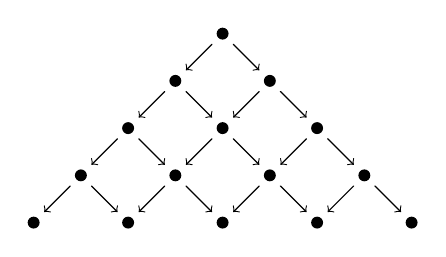
\begin{tikzpicture}[x=0.6cm,y=0.6cm,line cap=round]
		\fill (0,0) circle (0.5ex) coordinate (00);
		\fill (2,0) circle (0.5ex) coordinate (01);
		\fill (4,0) circle (0.5ex) coordinate (02);
		\fill (6,0) circle (0.5ex) coordinate (03);
		\fill (8,0) circle (0.5ex) coordinate (04);
		\fill (1,1) circle (0.5ex) coordinate (10);
		\fill (3,1) circle (0.5ex) coordinate (11);
		\fill (5,1) circle (0.5ex) coordinate (12);
		\fill (7,1) circle (0.5ex) coordinate (13);
		\fill (2,2) circle (0.5ex) coordinate (20);
		\fill (4,2) circle (0.5ex) coordinate (21);
		\fill (6,2) circle (0.5ex) coordinate (22);
		\fill (3,3) circle (0.5ex) coordinate (30);
		\fill (5,3) circle (0.5ex) coordinate (31);
		\fill (4,4) circle (0.5ex) coordinate (40);
		\draw[to-,shorten <=1.25ex,shorten >=1.25ex] (00) -- (10);
		\draw[to-,shorten <=1.25ex,shorten >=1.25ex] (01) -- (10);
		\draw[to-,shorten <=1.25ex,shorten >=1.25ex] (01) -- (11);
		\draw[to-,shorten <=1.25ex,shorten >=1.25ex] (02) -- (11);
		\draw[to-,shorten <=1.25ex,shorten >=1.25ex] (02) -- (12);
		\draw[to-,shorten <=1.25ex,shorten >=1.25ex] (03) -- (12);
		\draw[to-,shorten <=1.25ex,shorten >=1.25ex] (04) -- (13);
		\draw[to-,shorten <=1.25ex,shorten >=1.25ex] (10) -- (20);
		\draw[to-,shorten <=1.25ex,shorten >=1.25ex] (11) -- (20);
		\draw[to-,shorten <=1.25ex,shorten >=1.25ex] (11) -- (21);
		\draw[to-,shorten <=1.25ex,shorten >=1.25ex] (13) -- (22);
		\draw[to-,shorten <=1.25ex,shorten >=1.25ex] (12) -- (21);
		\draw[to-,shorten <=1.25ex,shorten >=1.25ex] (30) -- (40);
		\draw[to-,shorten <=1.25ex,shorten >=1.25ex] (31) -- (40);
		\draw[to-,shorten <=1.25ex,shorten >=1.25ex] (03) -- (13);
		\draw[to-,shorten <=1.25ex,shorten >=1.25ex] (12) -- (22);
		\draw[to-,shorten <=1.25ex,shorten >=1.25ex]  (21) -- (31);
		\draw[to-,shorten <=1.25ex,shorten >=1.25ex]  (22) -- (31);
		\draw[to-,shorten <=1.25ex,shorten >=1.25ex]  (20) -- (30);
		\draw[to-,shorten <=1.25ex,shorten >=1.25ex] (21) -- (30);
		\node[rotate=-45] at (2,1) {\pullbacksign};
		\node[rotate=-45] at (4,1) {\pullbacksign};
		\node[rotate=-45] at (6,1) {\pullbacksign};
		\node[rotate=-45] at (3,2) {\pullbacksign};
		\node[rotate=-45] at (5,2) {\pullbacksign};
		\node[rotate=-45] at (4,3) {\pullbacksign};
	\end{tikzpicture}
\end{center}
in $\Cc$ (shown here for $n=3$), and to be in $Q_n(\Cc)$ we require that all squares are pullbacks as indicated. Note that then in fact all rectangles you can find in this picture must be pullbacks.

The $Q_n(\Cc)$ assemble into a simplicial $\infty$-category $Q(\Cc)\colon \IDelta^\op\morphism \Cat_\infty$. To see this, one first shows that $\Fun(\TwAr([-])^\op,\Cc)\colon \IDelta^\op\morphism \Cat_\infty$ gives a functor. It's clear that all its ingredients are functorial, except perhaps for $\TwAr(-)$. But $\TwAr(-)\colon \sSet\morphism \sSet$ is right-adjoint to $(-)^\op\star (-)\colon \sSet\morphism \sSet$ (indeed, this guy has a right adjoint by \cref{thm:2Yoneda}, now unravel that $\TwAr(-)$ as defined in \cref{par:HomC}\itememph{b} fits the general description of such right adjoints), which one can show is a left Quillen functor for the Joyal model structure (by \cite[Proposition~D.5]{HigherCatsII} for example).

Now that we know $\Fun(\TwAr([-])^\op,\Cc)\colon \IDelta^\op\morphism \Cat_\infty$ is a functor, we only need to check that all the boundary and degeneracy maps preserve the full subcategories $Q_n(\Cc)$ described above. We leave this as an exercise. As you might have guessed, assigning to $\Cc$ the simplicial $\infty$-category $Q(\Cc)$ is called the \emph{Quillen $Q$-construction}.
\begin{propdef}\upshape\lecture[A sleep-deprived Fabian proves that $Q(\Cc)$ is a Segal $\infty$-category and introduces cartesian monoids.]{2020-11-24}\label{propdef:SpanQ}\itshape
	Let $\Cc$ be an $\infty$-category with pullbacks. The simplicial anima
	\begin{equation*}
		\core Q(\Cc)\colon \IDelta^\op\morphism \An
	\end{equation*}
	is a complete Segal space. Its associated category $\Span(\Cc)\simeq \asscat(\core Q(\Cc))$ is called the \emph{$\infty$-category of spans in $\Cc$}.
\end{propdef}
\begin{proof}
	We will actually prove that $Q(\Cc)$ itself satisfies the Segal and completeness conditions for simplicial $\infty$-categories rather than anima (really what this says is that there's an \emph{$\infty$-double category} $\Span^{(2)}(\Cc)$, but never mind that). Then all assertions for $\core Q(\Cc)$ will follow from the fact that $\core\colon \Cat_\infty\morphism\An$ preserves limits as it is a right-adjoint.
	
	Recall that the $0$-simplices in $\TwAr([n])^\op$ are given by morphisms in the poset $[n]$, i.e.\ by relations $(i\leq j)$. Now let $J_n\subseteq \TwAr([n])^\op$ be the subposet spanned by all $0$-simplices $(i\leq j)$ with $j\leq i+1$. In pictures, $J_n$ (for $n=3$) looks as follows:
	\begin{center}
		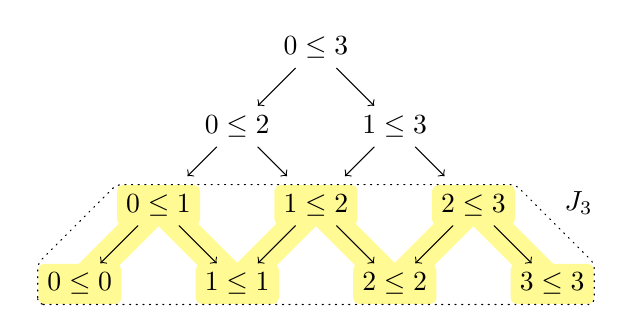
\begin{tikzpicture}[x=1cm,y=1cm,line cap=round, line join=round]
			\draw[line width=2.5ex,yellow!42!white] (0,0) to (1,1) to (2,0) to (3,1) to (4,0) to (5,1) to (6,0);
			\node[fill=yellow!42!white,rounded corners=2] (00) at (0,0) {$0\leq 0$};
			\node[fill=yellow!42!white,rounded corners=2] (01) at (2,0) {$1\leq 1$};
			\node[fill=yellow!42!white,rounded corners=2] (02) at (4,0) {$2\leq 2$};
			\node[fill=yellow!42!white,rounded corners=2] (03) at (6,0) {$3\leq 3$};
			\node[fill=yellow!42!white,rounded corners=2] (10) at (1,1) {$0\leq 1$};
			\node[fill=yellow!42!white,rounded corners=2] (11) at (3,1) {$1\leq 2$};
			\node[fill=yellow!42!white,rounded corners=2] (12) at (5,1) {$2\leq 3$};
			\node (20) at (2,2) {$0\leq 2$};
			\node (21) at (4,2) {$1\leq 3$};
			\node (30) at (3,3) {$0\leq 3$};
			\draw[to-] (00) -- (10);
			\draw[to-] (01) -- (10);
			\draw[to-] (01) -- (11);
			\draw[to-] (02) -- (11);
			\draw[to-] (02) -- (12);
			\draw[to-] (03) -- (12);
			\draw[to-,shorten <=1ex] (10) -- (20);
			\draw[to-,shorten <=1ex] (11) -- (20);
			\draw[to-,shorten <=1ex] (11) -- (21);
			\draw[to-,shorten <=1ex] (12) -- (21);
			\draw[to-]  (20) -- (30);
			\draw[to-] (21) -- (30);
			%\path (03.north east) to node {$J_3$} (12.north east);
			\draw[dotted,rounded corners=2] (00.south west) to (03.south east) to (03.north east) to node[above right] {$J_3$} (12.north east) to (10.north west) to node[above left] {$\phantom{J_n}$} (00.north west) to cycle;
		\end{tikzpicture}
	\end{center}
	Then one checks from the pointwise formula for Kan extensions (\cref{thm:KanExtension}) that a functor $F\colon \TwAr([n])^\op\morphism \Cc$ is in $Q_n(\Cc)$ iff it is right-Kan extended from $F|_{J_n}$. To see this in the example above, note that Kan extensions can be computed in steps (because right adjoints compose), so we may first Kan extend to the $0$-simplex $(0\leq 2)$, then to $(1\leq 3)$ and then finally to $(0\leq 3)$. In each step, the Kan extension is given by pullback, as one can see by restricting the limit from \cref{thm:KanExtension} to a suitable cofinal sub-$\infty$-category of the respective slice categories. The case for general $n$ works precisely the same. 
	
	In particular, since $J_n\subseteq \TwAr([n])^\op$ is fully faithful, we see that restriction to $J_n$ induces an equivalence
	\begin{equation*}
		Q_n(\Cc)\isomorphism \Fun(J_n,\Cc)
	\end{equation*}
	by \cref{cor:FullyFaithfulKanExtension}. The reason we don't work with the $J_n$ right away is that they do not form a cosimplicial $\infty$-category! So we have to include some redundant junk. However, the $J_n$ are closed under the maps induced by the Segal maps $e_i\colon [1]\morphism {[n]}$ (sending $[1]$ to $\{i,i+1\}\subseteq [n]$). These maps induce an equivalence $J_n\simeq J_1\sqcup_{J_0}\dotsb\sqcup_{J_0}J_1$ in $\Cat_\infty$, hence 
	\begin{align*}
		Q_n(\Cc)\simeq \Fun(J_1\sqcup_{J_0}\dotsb\sqcup_{J_0}J_1,\Cc)&\simeq \Fun(J_1,\Cc)\times_{\Fun(J_0,\Cc)}\dotsb\times_{\Fun(J_0,\Cc)}\Fun(J_1,\Cc)\\
		&\simeq Q_1(\Cc)\times_{Q_0(\Cc)}\dotsb\times_{Q_0(\Cc)}Q_1(\Cc)
	\end{align*}
	by \cref{cor:HomPreservesColimits}, which proves that $Q(\Cc)$ is indeed a Segal object in $\Cat_\infty$.
	
	For completeness, we have to check the condition from \cref{thmdef:RezkNerve}\itememph{b}, i.e.\ we need to show that
	\begin{equation*}
		\begin{tikzcd}[column sep=6em]
			Q_0(\Cc)\dar["s"']\rar["\Delta"]\drar[pullback]& Q_0(\Cc)\times Q_0(\Cc)\dar["{(s,s)}"]\\
			Q_3(\Cc)\rar["{\left(d_{\{0,2\}},d_{\{1,3\}}\right)}"]& Q_1(\Cc)\times Q_1(\Cc)
		\end{tikzcd}
	\end{equation*}
	is cartesian. So let $P$ be the pullback. We first check that the induced map $Q_0(\Cc)\morphism P$ is fully faithful. To see this, first note that the canonical map $\TwAr([n])^\op\morphism \TwAr([0])^\op$ induces a fully faithful map $s\colon \Fun(\TwAr([0])^\op,\Cc)\morphism\Fun(\TwAr([n])^\op,\Cc)$ for all $n$. Indeed, $\TwAr([0])^\op\simeq *$ is an anima, hence $s$ factors over the full subcategory $\Fun(|\TwAr([n])^\op|,\Cc)$. But $|\TwAr([n])^\op|\simeq *$ because $\TwAr([n])^\op$ contains $(0\leq n)$ as an initial element, and now it's clear that $s$ is indeed fully faithful. Hence so is $s\colon Q_0(\Cc)\morphism Q_n(\Cc)$ for all $n$.
	
	In particular, this is true for $n=3$. Moreover, $P\morphism Q_3(\Cc)$ is fully faithful too because it is a pullback of the fully faithful map $(s,s)\colon Q_0(\Cc)\times Q_0(\Cc)\morphism Q_1(\Cc)\times Q_1(\Cc)$. Now the diagram
	\begin{equation*}
		\begin{tikzcd}
			Q_0(\Cc)\rar\drar["s"',""{sloped,above,name=A}]& P\dar\\
			& Q_3(\Cc)\ar[from=A,to=1-2,phantom,pos=0.4,"\scriptscriptstyle/\!/\!/"]
		\end{tikzcd}
	\end{equation*}
	and the corresponding two-out-of-three property for fully faithful maps show that $Q_0(\Cc)\morphism P$ is fully faithful too.
	
	Now for essential surjectivity. The actual image of $Q_0(\Cc)\morphism P$ consists of the constant diagrams $F\colon \TwAr([3])^\op\morphism \Cc$, hence (by an easy argument) the essential image contains all diagrams that map all edges to equivalences. To see that every $0$-simplex in $P$ is a diagram $F\colon \TwAr([3])^\op\morphism \Cc$ of that form, we have to show the following:
	\begin{center}
		\begin{tikzpicture}[x=1.25cm,y=1.25cm,line cap=round]
			\node (00) at (0,0) {$F(0\leq 0)$};
			\node (01) at (2,0) {$F(1\leq 1)$};
			\node (02) at (4,0) {$F(2\leq 2)$};
			\node (03) at (6,0) {$F(3\leq 3)$};
			\node (10) at (1,1) {$F(0\leq 1)$};
			\node (11) at (3,1) {$F(1\leq 2)$};
			\node (12) at (5,1) {$F(2\leq 3)$};
			\node (20) at (2,2) {$F(0\leq 2)$};
			\node (21) at (4,2) {$F(1\leq 3)$};
			\node (30) at (3,3) {$F(0\leq 3)$};
			\draw[to-] (00) to  node[pos=0.5,above left=-0.6ex] {$\scriptscriptstyle(1)$} (10);
			\draw[to-] (01) to  node[pos=0.5,above right=-0.6ex] {$\scriptscriptstyle(2)$} (10);
			\draw[to-] (01) to  node[pos=0.5,below right=-0.6ex] {$\scriptscriptstyle(4)$} (11);
			\draw[to-] (02) to  node[pos=0.5,below left=-0.6ex] {$\scriptscriptstyle(4)$} (11);
			\draw[to-] (02) to  node[pos=0.5,above left=-0.6ex] {$\scriptscriptstyle(2)$} (12);
			\draw[to-] (03) to  node[pos=0.5,above right=-0.6ex] {$\scriptscriptstyle(1)$} (12);
			\draw[to-] (10) to  node[pos=0.5,above left=-0.6ex] {$\scriptscriptstyle(1)$}  (20);
			\draw[to-] (11) to  node[pos=0.7,below left=-0.6ex] {$\scriptscriptstyle(3)$} (20);
			\draw[to-] (11) to  node[pos=0.7,below right=-0.6ex] {$\scriptscriptstyle(3)$} (21);
			\draw[to-] (12) to  node[pos=0.5,above right=-0.6ex] {$\scriptscriptstyle(1)$} (21);
			\draw[to-]  (20) to  node[pos=0.5,above left=-0.6ex] {$\scriptscriptstyle(1)$}  (30);
			\draw[to-] (21) to  node[pos=0.5,above right=-0.6ex] {$\scriptscriptstyle(1)$}  (30);
			\draw[-to,dashed,bend right=35,FabiansPink] (30) to (10);
			\draw[-to,dashed,bend left=35,FabiansPink] (30) to (12);
			\draw[-to,dashed,bend right=35,FabiansPurple!67!FabiansPink] (20) to (00);
			\draw[-to,dashed,bend right=35,FabiansPurple!67!FabiansPink] (21) to (01);
			\draw[-to,dashed,bend left=35,FabiansPurple!67!FabiansPink] (20) to (02);
			\draw[-to,dashed,bend left=35,FabiansPurple!67!FabiansPink] (21) to (03);
			\node[rotate=-45] at (1.95,1.05) {\pullbacksign};
			\node[rotate=-45] at (4.05,1.05) {\pullbacksign};
			\node[rotate=-45] at (3,2.05) {\pullbacksign};
		\end{tikzpicture}
	\end{center}
	Suppose we are given a diagram $F\colon \TwAr([3])^\op\morphism \Cc$ in which all squares are pullbacks as indicated and such that the four dashed purple arrows are equivalences. Then all arrows are equivalences.
	
	Indeed, then the two dashed pink arrows $F(0\leq 3)\morphism F(0\leq 1)$ and $F(0\leq 3)\morphism F(2\leq 3)$ are equivalences as well, since they are pullbacks the purple arrows. By two-out-of-six, we see that all arrows labelled \enquote{$(1)$} must be equivalences.
	
	Now the commutative square
	\begin{equation*}
		\begin{tikzcd}
			F(0\leq 3)\rar[iso]\dar[iso]\drar[phantom,"\scriptscriptstyle/\!/\!/"] & F(1\leq 3)\dar[iso]\\
			F(0\leq 1)\rar & F(1\leq 1)
		\end{tikzcd}
	\end{equation*}
	shows that $F(0\leq 1)\morphism F(1\leq 1)$ is an equivalence. An analogous argument applies to $F(2\leq 3)\morphism F(2\leq 2)$. In other words, the two arrows labelled \enquote{$(2)$} are equivalences. This implies that the two arrows labelled \enquote{$(3)$} are equivalences, since they are pullbacks of the former. Finally, the two remaining arrows, labelled \enquote{$(4)$}, must be equivalences by two-out-of-three. We are done.
\end{proof}
	\renewcommand{\thechapter}{\Roman{chapter}}
	\chapter{Symmetric Monoidal and Stable \texorpdfstring{$\infty$}{infty}-Categories}\label{chap:Monoidal}
\setcounter{dummy}{-1}
\section{\texorpdfstring{$\IE_1$}{E1}-Monoids and \texorpdfstring{$\IE_1$}{E1}-Groups}
We start things off slowly by only considering (not necessarily symmetric) monoidal $\infty$-categories and $\IE_1$-spaces.
\numpar{Stasheff's Definition of Coherently Associative Monoids}
The naive way to define a monoid in $\An$ would be to have an object $M\in \An$ together with a multiplication map
\begin{equation*}
	\mu\colon M\times M\morphism M\,.
\end{equation*}
Now $\mu$ induces two different maps $M^3\morphism M$ (\enquote{two ways of bracketing}), so there ought to be a homotopy $H\colon \mu\circ (\mu\times \id_M)\simeq \mu\circ(\id_M\times \mu)$ between them. But then there are five maps $M^4\morphism M$ (\enquote{five ways of bracketing}), and we see that $H$ induces a loop in $\Hom_\An(M^4,M)$. Since $M$ should be associative up to \emph{coherent homotopy}, this loop has to be filled. The story goes on: There are a number of maps $M^5\morphism M$ (too lazy to count them) and now there are some $3$-simplices to be filled and so on.

Although this looks horrible, it is possible to turn these considerations into a precise definition, and one obtains Stasheff's \emph{$\IA_\infty$-spaces}. But we can take a simpler route! Indeed, thanks to our efforts so far, we now have the luxury of saying: \enquote{Well, a coherently associative monoid is just an $\infty$-category with only one object.} This leads to the following definition.
\begin{defi}\label{def:CartesianMonoids}
	Let $\Cc$ be an $\infty$-category with finite products (in particular, $\Cc$ has a final object $*\in \Cc$). A \emph{cartesian monoid in $\Cc$} is a functor $X\colon \IDelta^\op\morphism \Cc$ such that:
	\begin{alphanumerate}
		\item $X_0\simeq *$.
		\item It satisfies the Segal condition, i.e., the Segal maps $e_i\colon [1]\morphism {[n]}$ define an equivalence
		\begin{equation*}
			X_n\isomorphism \prod_{i=1}^nX_1
		\end{equation*}
	\end{alphanumerate}
	Let $\cat{Mon}(\Cc)\subseteq\cat{s}\Cc$ be the full sub-$\infty$-category spanned by cartesian monoids. If $\Cc=\An$, these are also called \emph{$\IE_1$-monoids}, \emph{$\IA_\infty$-spaces}, \emph{coherent monoids}, \emph{special $\Delta$-spaces}, \dotso. For $\Cc=\Cat_\infty$ we simply call them \emph{monoidal $\infty$-categories} (note that these can also be encoded as cocartesian fibrations over $\IDelta^\op$).
\end{defi}
To make sense of the condition from \cref{def:CartesianMonoids}\itememph{b}, note that since $X_0\simeq *$ is terminal, we have $X_1\times_{X_0}\times\dotsb\times_{X_0}X_1\simeq \prod_{i=1}^nX_1$, so this condition really \emph{is} the Segal condition. Somewhat weird though is that we don't impose any completeness conditions, and in fact, cartesian monoids in $\An$ are usually \emph{not} complete Segal spaces! This is in some sense fixed by the following proposition.
\begin{prop}\label{prop:CompletionOfMonoidsFullyFaithful}
	The completion functor $\comp\colon\cat{sAn}\morphism\cat{CSAn}$ from Lemma/Defi-nition~\textup{\labelcref{lemdef:Completion}} restricts to a fully faithful functor
	\begin{equation*}
		\comp\colon\cat{Mon}(\An)\morphism */\cat{CSAn}
	\end{equation*}
	with essential image those pointed complete segal spaces $(X,x)$ with $\pi_0X_0=*$.
\end{prop}
In other words, monoids really are categories with one object (up to equivalence, but not up to contractible choice, as Bastiaan pointed out in the lecture), since the target is also pointed categories with connected base.
\begin{proof}[Proof of \cref{prop:CompletionOfMonoidsFullyFaithful}]
	The proof is not hard, but quite lengthy, so we break it down into four major steps. Be aware that Step~\itememph{3} wasn't done in the lecture, so any errors in it are my fault.
	\begin{alphanumerate}
		\item[\itememph{1}] \itshape There exists a reasonable candidate $\decomp\colon {*/\cat{CSAn}}\morphism \cat{Mon}(\An)$ of an inverse functor \embrace{\enquote{decompletion}}.
	\end{alphanumerate}
	%Recall that if $X$ is Segal, then the completion functor does not affect the pullback spaces
	%\begin{equation*}
	%	\begin{tikzcd}
	%		P_{x,y}\rar\dar\drar[pullback] & X_1\dar["{(d_1,d_0)}"]\\
	%		*\rar["{(x,y)}"] & X_0\times X_0
	%	\end{tikzcd}
	%\end{equation*}
	%(this follows essentially from \cref{eq:asscat2}).
	
	If $(X,x)$ is a pointed complete Segal space, and if $Y\in \cat{Mon}(\An)$ is the \enquote{universal way} to make $(X,x)$ connected and still satisfy the Segal condition, then it's reasonable to expect that $Y_n$ sits inside a pullback
	\begin{equation*}
		\begin{tikzcd}[column sep=large]
			Y_n\dar\rar\drar[pullback]& X_n\dar\\
			*\rar["{(x,\dotsc,x)}"] & X_0^{n+1}
		\end{tikzcd}
	\end{equation*}
	for all $[n]\in \IDelta^\op$. We will see that this gives indeed the correct functor.
	
	Let's first address the elephant in the room, i.e.\ how to make the pointwise-defined $Y_n$ into a functor $Y\colon\IDelta^\op\morphism \An$, which in turn should be functorial in $X$. Since taking pullbacks is functorial, we'll have solved both problems at once if we show that the cospan diagram
	$*\morphism X_0^{n+1}\lmorphism X_n$ is functorial in $(X,x)$ and in $[n]$. To this end consider $X$ as a functor $\IDelta\morphism \An^\op$ and colimit-extend it to a functor
	\begin{equation*}
		|\blank|_X\colon \cat{sAn}\morphism \An^\op\,.
	\end{equation*}
	This can be done functorially in $X$, as \cref{thm:ColimitPreservingRepresentable} shows. In more abstract terms, what we do here is to identify  $\cat{sAn}\simeq \Fun(\IDelta,\An^\op)^\op\simeq \Fun^L(\cat{sAn},\An^\op)^\op$. We define two functors $\Delta,\Delta_0\colon \IDelta\morphism\cat{sSet}\subseteq\cat{sAn}$ via
	\begin{equation*}
		\Delta\big([n]\big)=\Delta^n\quad\text{and} \quad\Delta_0\big([n]\big)=\coprod_{i=0}^n\Delta^0\,. 
	\end{equation*}
	Since $\Delta$ and $\Delta_0$ are functors between $1$-categories (before we compose them with the inclusion $\cat{sSet}\subseteq \cat{sAn}$), we don't need to check any higher coherences and immediately obtain that $\Delta$ and $\Delta_0$ are indeed functors. Moreover, the canonical map $\coprod_{i=0}^n\Delta^0\morphism \Delta^n$ sending the $i\ordinalth$ component to the $i\ordinalth$ vertex of $\Delta^n$ is clearly functorial in $[n]\in \IDelta$, hence it induces a natural transformation $\Delta_0\Rightarrow\Delta$ (which exhibits $\Delta_0$ as the \enquote{$0$-skeleton} of $\Delta$, hence the notation). Now consider the two composites
	\begin{equation*}
		\cat{sAn}\simeq \Fun\left(\IDelta,\An^\op\right)^\op\simeq \Fun\left(\cat{sAn},\An^\op\right)^\op\doublemorphism[\Delta^*][\Delta_0^*]\Fun\left(\IDelta,\An^\op\right)^\op\simeq \cat{sAn}\,,
	\end{equation*}
	which we denote $|\Delta|_{(-)}$ and $|\Delta_0|_{(-)}$. The transformation $\Delta_0\Rightarrow \Delta$ induces a transformation $|\Delta|_{(-)}\Rightarrow |\Delta_0|_{(-)}$ going in the other direction, since there has been an $(-)^\op$ in between. Upon closer inspection, we find that $\Delta\colon \IDelta\morphism\cat{sAn}$ is actually nothing else but the Yoneda embedding, hence \cref{thm:ColimitPreservingRepresentable} shows that $|\Delta|_{(-)}\simeq \id$. Moreover, since $|\blank|_X$ preserves colimits, we easily obtain
	\begin{equation*}
		X_0^{n+1}\simeq \left|\coprod_{i=0}^n\Delta^0\right|_X\,,
	\end{equation*}
	hence the $X_0^{n+1}$ can be organized into a simplicial anima $|\Delta_0|_X$. The transformation $\id\simeq |\Delta|_{(-)}\Rightarrow |\Delta_0|_{(-)}$ gives a natural map $X\morphism |\Delta_0|_X$.
	
	This shows that the maps $X_0^{n+1}\lmorphism X_n$ can indeed be made functorial in $X$ and $[n]$. A similar argument applies shows that the maps $*\morphism X_0^{n+1}$, which assemble into a functorial map $\Delta^0\morphism |\Delta_0|_X$. We conclude that $Y\simeq X\times_{|\Delta_0|_X}\Delta^0$ as above is indeed a simplicial anima and functorial in $X$. We have $Y_0\simeq *$ by construction and also $Y_n\simeq Y_1\times_{Y_0}\dotsb\times_{Y_0}Y_1$ follows from the fact that $X$ itself satisfies the Segal conditions together with some abstract pullback nonsense (basically that \enquote{limits commute}, see the dual of \cref{prop:ColimitsCommute}). So $Y\in \cat{Mon}(\An)$ and we can finally write down the functor
	\begin{equation*}
		\decomp\colon {*/\cat{CSAn}}\morphism \cat{Mon}(\An)\,.
	\end{equation*}
	This finishes Step~\itememph{1}.
	\begin{alphanumerate}
		\item[\itememph{2}] \itshape The completion functor $\comp\colon \cat{Mon}(\An)\morphism \cat{CSAn}$ from \cref{lemdef:Completion} factors over $*/\cat{CSAn}\morphism \cat{CSAn}$ and its essential image is contained in those pointed complete Segal spaces $(X,x)$ with $\pi_0X_0=*$.
	\end{alphanumerate}
	
	To get the factorisation, observe that $\cat{Mon}(\An)$ has an initial object, namely $\Delta^0\in\sSet\subseteq\cat{sAn}$ (in the lecture we called it \enquote{$\const*$}, but it's really just $\Delta^0$). Indeed, if $T\in \cat{Mon}(\An)$, then
	\begin{equation*}
		\Hom_{\cat{Mon}(\An)}(\Delta^0,T)\simeq \Hom_{\cat{sAn}}(\Delta^0,T)\simeq T_0\simeq *
	\end{equation*}
	by \cref{def:CartesianMonoids}\itememph{a}. Also $\comp (\Delta^0)\simeq *$, so the completion functor really lifts to a functor $\cat{Mon}(\An)\simeq \Delta^0/\cat{Mon}(\An)\morphism */\cat{CSAn}$, as required.
	
	To check that $\pi_0(\comp T)_0=*$, recall that $(\comp T)_0\simeq \core \asscat T\simeq |T^\times|$ by \cref{eq:asscat1}. Now we have to use the following general fact:
	\begin{alphanumerate}
		\item[\itememph{*}] \itshape For all $X\in\cat{sAn}$ the map $\pi_0X_0\morphism \pi_0|X|$ is surjective.
	\end{alphanumerate}
	This shows what we want since $(T^\times)_0\simeq T_0\simeq *$ holds by assumption. To see where \itememph{*} comes from, observe that $\pi_0$, being a left adjoint (\cref{exm:MyFirstAdjoints}\itememph{a}), commutes with colimits. This shows $\pi_0|X|\simeq \pi_0\colimit_{\IDelta^\op}X\simeq \colimit_{\IDelta^\op}\pi_0X$, where the colimit on the right-hand side is a good old colimit taken in $\sSet$. Now $\{d_0,d_1\colon [1]\shortdoublemorphism [0]\}\subseteq \IDelta^\op$ is $1$-cofinal (but not $\infty$-cofinal!), hence
	\begin{equation*}
		\colimit_{\IDelta^\op}\pi_0X=\Coeq\left(\pi_0X_1\doublemorphism[d_1][d_0] \pi_0X_0\right)\,.
	\end{equation*}
	This immediately implies \itememph{*} and thus Step~\itememph{2} is done.
	\begin{alphanumerate}
		\item[\itememph{3}]\itshape The functors from Step~\itememph{1} and Step~\itememph{2} fit into an adjunction
		\begin{equation*}
			\comp\colon \cat{Mon}(\An)\doublelrmorphism {*/\cat{CSAn}}\noloc \decomp
		\end{equation*}
	\end{alphanumerate}
	
	Consider $T\in \cat{Mon}(\An)$, which is naturally pointed via the unique (up to contractible choice) map $1_T\colon \Delta^0\morphism T$, and let $(X,x)$ be a pointed complete Segal space. Then
	\begin{align*}
		\Hom_{*/\cat{CSAn}}\big(\comp T,(X,x)\big)&\simeq \Hom_{*/\cat{sAn}}\big((T,1_T),(X,x)\big)\\
		&\simeq \Hom_{\cat{sAn}}(T,X)\times_{\Hom_{\cat{sAn}}(\const 1_T,X)}\{\const x\}\\
		&\simeq \Hom_{\cat{sAn}}(T,X)\times_{\Hom_\An(1_T,X_0)}\{x\}\,.
	\end{align*}
	The first equivalence follows from \cref{lemdef:Completion} (and the fact that adjunctions extend to slice categories), the second follows from \cite[Corollary~VIII.6]{HigherCatsII}. The last one follows by inspection. All of them are functorial in $(X,x)$. Moreover, we have
	\begin{align*}
		\Hom_{\cat{Mon}(\An)}\big(T,\decomp (X,x)\big)&\simeq \Hom_{\cat{sAn}}\left(T,X\times_{|\Delta_0|_X}\Delta^0\right)\\
		&\simeq \Hom_{\cat{sAn}}(T,X)\times_{\Hom_{\cat{sAn}}(T,|\Delta_0|_X)}\Hom_{\cat{sAn}}(T,\Delta^0)\,.
	\end{align*}
	Since $\id\Rightarrow |\Delta_0|_{(-)}$ is a natural transformation, one quickly checks that the morphism $\Hom_{\cat{sAn}}(T,X)\morphism \Hom_{\cat{sAn}}(T,|\Delta_0|_X)$ factors over $\Hom_{\cat{sAn}}(|\Delta_0|_T,|\Delta_0|_X)$. But $T_0\simeq *$, hence $|\Delta_0|_T\simeq \Delta^0$. Also $\Hom_{\cat{sAn}}(T,\Delta^0)\simeq *$. Putting everything together, we can rewrite
	\begin{equation*}
		\Hom_{\cat{Mon}(\An)}\big(T,\decomp (X,x)\big)\simeq \Hom_{\cat{sAn}}(T,X)\times_{\Hom_\An(T_0,X_0)}\{x\}\,,
	\end{equation*} 
	and after another inspection, we see that our calculations of $\Hom_{*/\cat{CSAn}}(\comp T,(X,x))$ and $\Hom_{\cat{Mon}(\An)}(T,\decomp (X,x))$ agree, as they are supposed to. This finishes Step~\itememph{3}.
	\begin{alphanumerate}
		\item[\itememph{4}] \itshape The restriction $\decomp\colon (*/\cat{CSAn})_{\pi_0=*}\morphism \cat{Mon}(\An)$ is indeed an inverse to $\comp$, where $(*/\cat{CSAn})_{\pi_0=*}\subseteq */\cat{CSAn}$ denotes the full subcategory spanned by those $(X,x)$ with $\pi_0X_0=*$.
	\end{alphanumerate}
	
	Thanks to Step~\itememph{3}, we already have unit and counit transformations $\id\Rightarrow \decomp\circ \comp$ and $\comp\circ\decomp\Rightarrow \id$, so we only need to show that they are equivalences. Let's start with the counit. We must show
	\begin{equation*}
		\comp\big(\decomp (X,x)\big)\simeq (X,x)
	\end{equation*}
	for all $(X,x)\in (*/\cat{CSAn})_{\pi_0=*}$. Observe that $\comp X\simeq X$ because $X$ is already complete. Hence it suffices to show $\asscat(\decomp(X,x))\simeq \asscat X$ (and check that the chosen base points on both sides correspond, but that's easy) because $\comp\simeq \N^r\circ \asscat$ by \cref{lemdef:Completion} and $\N^r$ is fully faithful by \cref{thmdef:RezkNerve}. Using \cref{eq:asscat1} and the fact that $X^\times$ is a constant simplicial anima with value $X_0$ as $X$ is complete, we see that
	\begin{equation*}
		\pi_0\core(\asscat X)\simeq \pi_0|X^\times|\simeq \pi_0X_0\simeq *\,,
	\end{equation*}
	so $\asscat(\decomp(X,x))\morphism \asscat X$ is essentially surjective for trivial reasons. Moreover, we have $\decomp(X,x)_0\simeq \{x\}$ by construction, and \cref{eq:asscat2} (which is applicable here because $\decomp(X,x)$ is Segal by construction) easily shows
	\begin{equation*}
		\Hom_{\asscat(\decomp(X,x))}(x,x)\simeq P_{x,x}\simeq \Hom_{\asscat X}(x,x)\,,
	\end{equation*}
	so $\asscat(\decomp(X,x))\morphism \asscat(X)$ is fully faithful too. This shows that the counit is an equivalence, as claimed. The argument for the unit is similar: We have to show
	\begin{equation*}
		T\simeq \decomp(\comp T)
	\end{equation*}
	for all $T\in \cat{Mon}(\An)$. Since both sides are functors $\IDelta^\op\morphism \cat{An}$ and a natural transformation between them is already given, we can do this degree-wise by \cref{thm:JoyalEquivalence}\itememph{b}. Since both sides are cartesian monoids, is suffices to check that the map in degree $1$ is an equivalence, i.e.\ that $T_1\simeq \decomp(\comp T)_1$. Write $(X,x)\simeq \comp T$. By construction we have
	\begin{equation*}
		\decomp(X,x)_1\simeq P_{x,x}\quad\text{and}\quad T_1\simeq P_{1_T,1_T}\,,
	\end{equation*}
	where as usual $1_T\colon \Delta^0\morphism T$ is the natural pointing of $T$. As observed at the very beginning of this proof, the spaces $P_{y,z}$ aren't affected by completion, hence $P_{x,x}\simeq P_{1_T,1_T}$ and we're done. 
\end{proof}
\lecture[More on $\IE_1$-monoids and $\IE_1$-groups. Group completion.\newline --- \emph{\enquote{The fact that you can write down a group or a monoid in semester 2 is sort of an accident.}}]{2020-11-26}Under the equivalence $\Cat_\infty\simeq \cat{CSAn}$ from \cref{thmdef:RezkNerve}, the construction of $\decomp$ from the proof of \cref{prop:CompletionOfMonoidsFullyFaithful} corresponds to a functor $*/\Cat_\infty\morphism\cat{Mon}(\An)$ which becomes an equivalence when restricted to the full subcategory $(*/\Cat_\infty)_{\geq 1}\subseteq */\Cat_\infty$ spanned by those $\Cc$ with $\pi_0\core\Cc\simeq *$. In diagrams,
\begin{equation*}
	\begin{tikzcd}
		*/\Cat_\infty\rar & \cat{Mon}(\An)\\
		(*/\Cat_\infty)_{\geq 1}\uar[symbol=\subseteq]\urar[iso] & 
	\end{tikzcd}
\end{equation*}
Explicitly, this functor sends a pointed $\infty$-category $(\{x\}\morphism \Cc)$ to $\Hom_\Cc(x,x)$ in degree $1$ (and then all other degrees are determined by the conditions from \cref{def:CartesianMonoids}). We thus obtain:
\begin{cor}
	If $\Cc$ is an $\infty$-category and $x\in \Cc$, then $\Hom_\Cc(x,x)$ carries a canonical structure of an $\IE_1$-monoid.
\end{cor}
\begin{defi}\label{def:E1Group}
	Let $\Cc$ be an $\infty$-category with finite products. A cartesian monoid $X$ in $\Cc$ is called a \emph{cartesian group} (or \emph{$\IE_1$-group} in the case $\Cc=\An$) if the map
	\begin{align*}
		(\pr_1,\circ)\colon X_1\times X_1&\isomorphism X_1\times X_1\\
		(f,g)&\longmapsto (f,f\circ g)
	\end{align*}
	is an equivalence. Here \enquote{$\circ$} is the composition as defined in \cref{thmdef:RezkNerve}\itememph{c}. We denote by $\Grp(\Cc)\subseteq \cat{Mon}(\Cc)$ the full sub-$\infty$-category of cartesian groups.
\end{defi}
\begin{prop}\label{prop:Grp(An)=(*/An)Connected}
	The equivalences $\cat{Mon}(\An)\simeq (*/\Cat_\infty)\simeq (*/\cat{CSAn})_{\pi_0=*}$ restrict to equivalences
	\begin{equation*}
		\begin{tikzcd}[column sep=small]
			\cat{Mon}(\An)\dar[iso]\rar[symbol=\supseteq] & \Grp(\An)\dar[iso]\\
			(*/\Cat_\infty)_{\geq 1}\dar[iso] \rar[symbol=\supseteq] & (*/\An)_{\geq 1}\dar[iso]\\
			(*/\cat{CSAn})_{\pi_0=*}\rar[symbol=\supseteq] & (*/\cat{sAn}_{\mathrm{const}})_{\pi_0=*}
		\end{tikzcd}
	\end{equation*}
	In the lower right corner we use the notation from \cref{exm:MyFirstRezkNerves}\itememph{c}.
\end{prop}
\begin{proof}[Proof sketch]
	In the lecture we noted only that $X\in \cat{Mon}(\An)$ is an $\IE_1$-group iff the set $\pi_0X_1$ with its induced ordinary monoid structure is an ordinary group.
	
	To elaborate on this a bit more, first note that we may assume $X\simeq \Hom_\Cc(x,x)$ for some $\infty$-category $\Cc$ with $\pi_0\core \Cc\simeq *$, as was argued above. If $X$ is an $\IE_1$-group, then $\pi_0\Hom_\Cc(x,x)$ must be an ordinary group, which implies that all endomorphisms of $x$ are equivalences, hence all morphisms in $\Cc$ are equivalences as $\pi_0\core \Cc\simeq *$. This proves that $\Cc$ is an anima by \cref{thm:JoyalLifting}. Conversely, if $\Cc$ is an anima, either inclusion $[1]\monomorphism J$ into the free-living isomorphism induces a trivial fibration $\Fun(J,\Cc)\isomorphism \Ar(\Cc)$. Choosing a section and composing it with the the other map $\Fun(J,\Cc)\morphism \Ar(\Cc)$ (induced by the other inclusion $[1]\monomorphism J$) yields an \enquote{inversion} map $(-)^{-1}\colon \Hom_\Cc(x,x)\morphism \Hom_\Cc(x,x)$. From this we can construct an inverse of the map in \cref{def:E1Group}
\end{proof}
\numpar{Some Explicit Calculations}\label{par:Grp(An)=(*/An)Connected}
The equivalence $\Grp(\An)\simeq (*/\An)_{\geq 1}$ is explicitly given as follows:
\begin{equation*}
	B=|\blank|\colon \Grp(\An)\doublelrmorphism[\sim][\sim](*/\An)_{\geq 1}\noloc \Omega\,.
\end{equation*}
The use $B$ to denote the functor $|\blank| = \colimit_{\IDelta^\op}$ is common in the literature, as it is short for \enquote{bar construction}. Fabian doesn't like it, since he finds it stupid to name something after the way it was typeset in the pre-\LaTeX\ age (where people had to resort to bars to denote their tensor products). Amusingly though, his preferred notation consists of actual bars \dotso In these notes, however, I'll show my bad taste and consistently use $B$.


Anyway, back to the matters at hand. To make sense of why the above equivalence is indeed given by $B=|\blank|$ and $\Omega$, recall that the composition
\begin{equation*}
	\cat{Mon}(\An)\xrightarrow{\comp}\cat{CSAn}\morphism[\ev_0]\An
\end{equation*}
sends $X\mapsto |X^\times|$, as follows from \cref{eq:asscat1} and some unravelling. If $X$ is an $\IE_1$-group, one easily verifies $X^\times=X$ and thus $X\in \Grp(\An)$ is sent to $BX=|X|$, as claimed. Conversely, the composition
\begin{equation*}
	(*/\An)_{\geq 1}\xrightarrow{\decomp}\Grp(\An)\morphism[\ev_1]\An
\end{equation*}
sends a pointed connected anima $(K,k)$ to $\Hom_K(k,k)$, as argued previously. So to justify why $(*/\An)_{\geq 1}\isomorphism \Grp(\An)$ should be thought of as a \enquote{loop space functor}, we must explain why $\Omega_kK\simeq \Hom_K(k,k)$. This can be done by several arguments and I will present a different one than in the lecture. The loop space is usually defined by the left of the following pullback diagrams in $\An$:
\begin{equation*}
	\begin{tikzcd}
		\Omega_kK\vphantom{\Hom_K^L}\dar\rar\drar[pullback]& *\vphantom{K_{k/}}\dar["k"]\\
		*\rar["k"] & K
	\end{tikzcd}\quad\isomorphism\quad
	\begin{tikzcd}
		\Hom_K^L(k,k)\dar\rar\drar[pullback]& K_{k/}\dar\\
		*\rar["k"]& K
	\end{tikzcd}
\end{equation*}
The map $*\morphism K$ can be factored into the left anodyne map $*\monomorphism K_{k/}$ followed by the left fibration $K_{k/}\morphism K$, which is even a Kan fibration since $K$ is an anima. Replacing one of the $*\morphism K$ accordingly, we obtain the pullback diagram on the right, which is already a pullback in $\sSet$ as one leg is a Kan fibration (see \cref{thm:HomotopyLimits}). Its pullback is thus $\Hom_K^L(k,k)\simeq \Hom_K(k,k)$ as left-$\Hom$ anima coincide with the regular $\Hom$ anima by \cite[Digression~I Corollary~D.2]{HigherCatsII}.

In particular, we have proved another result from algebraic topology (or rather deduced it from the much more general statement of \cref{thmdef:RezkNerve}, which we didn't prove, but never mind that).
\begin{cor}[Recognition Principle for Loop Spaces, Stasheff]
	The loop functor $\Omega\colon {*/\An}\morphism \An$ lifts to an equivalence
	\begin{equation*}
		\Omega\colon (*/\An)_{\geq 1}\isomorphism \Grp(\An)\,.
	\end{equation*}
\end{cor}
Note that $\ev_1\colon \cat{Mon}(\An)\morphism \An$ preserves limits since $\cat{Mon}(\An)$ is closed under limits in $\cat{sAn}$ (the Segal condition is given by a limit and limits commute by the dual of \cref{prop:ColimitsCommute}). Colimits however are bloody complicated, and even though one can show that $\cat{Mon}(\An)$ is cocomplete, colimits in it are \emph{by far not} just colimits of underlying simplicial anima, same as colimits of ordinary monoids are much more complicated than colimits in sets.
\begin{prop}\label{prop:InftyGrp}
	The inclusion $\Grp(\An)\subseteq\cat{Mon}(\An)$ has a left adjoint called \emph{group completion} and denoted
	\begin{equation*}
		(-)^\inftygrp\colon \cat{Mon}(\An)\morphism \Grp(\An)\,.
	\end{equation*}
	It is given by $X^\inftygrp\simeq \Omega BX$, where $B\colon \Mon(\An)\morphism ({*/\An})_{\geq 1}$ denotes a functor extending the $B$ from \cref{par:Grp(An)=(*/An)Connected}.
\end{prop}
\begin{proof}
	We know that $\An\subseteq \Cat_\infty$ has a left-adjoint $|\blank|\colon \Cat_\infty\morphism \An$. The unit and counit are equivalences on $*\in \An$, hence the adjunction passes to slices under it. Moreover the $(-)_{\geq 1}$-parts on both sides are clearly preserved, thus $|\blank|$ descends to a left adjoint
	\begin{equation*}
		|\blank|\colon (*/\Cat_\infty)_{\geq 1}\morphism (*/\An)_{\geq 1}
	\end{equation*}
	of the obvious inclusion in the other direction. Now use \cref{prop:Grp(An)=(*/An)Connected} to get the desired left-adjoint $(-)^\inftygrp\colon \cat{Mon}(\An)\morphism\Grp(\An)$. The explicit description follows from our calculations in \cref{par:Grp(An)=(*/An)Connected}, and \cref{rem:Realisation}, which ensures that the different meanings of $|\blank|$ ($\colimit_{\IDelta^\op}$ or localisation of an $\infty$-category at all its morphisms) are actually compatible.
\end{proof}
A consequence that wasn't explicitly mentioned, but used later in the course, is the following:
\begin{cor*}\label{cor*:BOmegaAdjunction}
	Without restricting them as in \cref{par:Grp(An)=(*/An)Connected}, the functors $B$ and $\Omega$ form an adjunction
	\begin{equation*}
		B\colon \Mon(\An)\doublelrmorphism {*/\An}\colon \Omega\,.
	\end{equation*}
\end{cor*}
\begin{proof*}
	For a pointed anima $(X,x)$, let $X_x$ denote the connected component containing $x$. Then $\Omega_xX\simeq \Omega_xX_x$, so the equivalence $\Omega\colon (*/\An)_{\geq 1}\isomorphism\Grp(\An)$ from \cref{par:Grp(An)=(*/An)Connected} extends to a functor $\Omega\colon {*/\An}\morphism \Grp(\An)$. Now if $M\in \Mon(\An)$ is an $\IE_1$-monoid, we can compute
	\begin{align*}
		\Hom_{\Mon(\An)}(M,\Omega_xX)&\simeq \Hom_{\Grp(\An)}(M^\inftygrp,\Omega_xX_x)\\
		&\simeq \Hom_{\Grp(\An)}\big(\Omega BM,\Omega_xX_x\big)\\
		&\simeq \Hom_{(*/\An)_{\geq 1}}\big(BM,X_x\big)\\
		&\simeq \Hom_{*/\An}\big(BM,X\big)\,,
	\end{align*}
	which establishes the desired adjunction. The second equivalence follows from \cref{prop:InftyGrp}, the third equivalence uses that $\Omega\colon (*/\An)_{\geq 1}\isomorphism\Grp(\An)$ is an equivalence, and the fourth equivalence follows from the fact that $BM$ is connected (by construction), hence any pointed map $BM\morphism X$ only hits the connected component $X_x$.
\end{proof*}
Next we will discuss some examples. We begin with free monoids and groups.
\begin{prop}\label{prop:FreeMonoids}
	The evaluation functor $\ev_1\colon \cat{Mon}(\An)\morphism \An$ has a left adjoint $\operatorname{Free}^{\Mon}\colon \An\morphism \cat{Mon}(\An)$. It is given explicitly by the \enquote{anima of words of arbitrary length}
	\begin{equation*}
		\operatorname{Free}^{\Mon}(K)_1\simeq \coprod_{n\geq 0}K^n\,.
	\end{equation*}
\end{prop}
\begin{proof*}
	We didn't prove this in the lecture, but here's a very simple argument that Fabian explained to me. We call a morphism in $\IDelta$ \emph{inert} if it is the inclusion of an interval, and \emph{active} if it preserves the largest and the smallest element. Note that the Segal maps $e_i\colon [1]\morphism {[n]}$ are precisely the inert maps with source $[1]$, and that every map can be uniquely factored into an inert followed by an active. We let $\IDelta^\op_\mathrm{int}\subseteq \IDelta^\op$ denote the (non-full) subcategory spanned by the inert maps. Let's first verify the following two claims.
	\begin{alphanumerate}
		\item[\itememph{1}] \itshape Consider the full sub-$\infty$-category $\Fun^\mathrm{Seg}(\IDelta^\op_\mathrm{int},\An)$ spanned by the \enquote{reduced Segal functors}, i.e.\ those $X\colon \IDelta^\op_\mathrm{int}\morphism \An$ satisfying $X_0\simeq *$ and $X_n\simeq \prod_{i=1}^nX_1$ via the Segal maps. Then evaluation at $[1]$ induces an equivalence
		\begin{equation*}
			\ev_{1}\colon \Fun^\mathrm{Seg}(\IDelta^\op_\mathrm{int},\An)\isomorphism \An\,.
		\end{equation*}
		\item[\itememph{2}] Consider the left-Kan extension functor $\Lan_i\colon \Fun(\IDelta^\op_\mathrm{int},\An)\morphism \Fun(\IDelta^\op,\An)$ along $i\colon \IDelta^\op_\mathrm{int}\morphism \IDelta^\op$.Then $\Lan_i$ preserves reduced Segal functors.
	\end{alphanumerate}
	To show \itememph{1}, we verify that right-Kan extension along the inclusion $j\colon \{[1]\}\morphism \IDelta_\mathrm{int}^\op$ defines an inverse. Using the pointwise formulas from \cref{thm:KanExtension} together with the fact that the inert maps $[1]\morphism{[n]}$ are precisely the Segal maps, we see that $\Ran_j$ indeed takes values in the reduced Segal functors, and that $\Ran_j\circ \ev_{1}\simeq \id$. To show $\ev_{1}\circ \Ran_j\simeq \id$, observe that $j$ is fully faithful and use \cref{cor:FullyFaithfulKanExtension}. This proves \itememph{1}.
	
	To prove \itememph{2}, let $X\colon \IDelta^\op_\mathrm{int}\morphism \An$ be reduced Segal. By \cref{thm:KanExtension},
	\begin{equation*}
		(\Lan_iX)_n\simeq \colimit_{([k]\morphism{ [n]})\in \IDelta^\op_\mathrm{int}/[n]}X_k\simeq \colimit_{([k]\morphism {[n]})\in \IDelta^\op_\mathrm{int}/[n]} X_1^k\,.
	\end{equation*}
	An object $[k]\morphism {[n]}$ of $\IDelta^\op_\mathrm{int}/[n]$ corresponds to a map $[n]\morphism{} [k]$ in $\IDelta$. Any such map can be uniquely factored into an inert $[n']\morphism{} [k]$ followed by an active $\alpha\colon [n]\morphism{} [n']$. This allows us to decompose $\IDelta^\op_\mathrm{int}/[n]$ into a disjoint union $\coprod_\alpha \Cc_\alpha$, indexed by all active maps $\alpha\colon [n]\morphism {[n']}$ with source $[n]$. Moreover, each $\Cc_\alpha$ has a terminal object, which is given by $\alpha$ itself (or rather the corresponding object $\alpha^\op\colon[n']\morphism{[n]}$ in $\IDelta^\op_\mathrm{int}/[n]$).
	
	For $n=0$ this shows $(\Lan_iX)_n\simeq *$, since $\id_{[0]}\colon [0]\morphism {[0]}$ is the only active map with source $[0]$. For $n=1$, we get a unique active map $[1]\morphism {[n]}$ for all $n$, which shows $(\Lan_iX)_1\simeq \coprod_{k\geq 0}X_1^k$. For general $n$, we get
	\begin{equation*}
		(\Lan_iX)_n\simeq \coprod_{k_1,\dotsc,k_n\geq 0} X_1^{k_1+\dotsb +k_n}\,.
	\end{equation*}
	Upon inspection, this shows that $\Lan_iX$ is again reduced Segal. We've thus proved~\itememph{2}. Combining \itememph{1} and~\itememph{2} shows that $\Free^\Mon\colon \An\morphism \Mon(\An)$ is given by $\Lan_i\circ \Ran_j$. But then the calculations above show $\operatorname{Free}^{\Mon}(K)_1\simeq \coprod_{n\geq 0}K^n$, as claimed.
\end{proof*}
%We postpone the proof of \cref{prop:FreeMonoids} indefinitely (but Fabian's notes give a sketch in the much more general setting of algebras over $\infty$-operads, see \cite[Chapter~II pp.~128--132]{KTheory}). 
By the explicit construction of $\Free^\Mon$, the diagram
\begin{equation*}
	\begin{tikzcd}[column sep=large]
		\Set\dar\rar["\operatorname{Free}"]& \cat{Mon}(\Set)\dar\\
		\An\rar["\operatorname{Free}^{\Mon}"] & \cat{Mon}(\An)
	\end{tikzcd}
\end{equation*}
commutes. But be aware that this is not automatic, and in fact we'll see it very much breaks once we impose commutativity (see pages~\labelcpageref{par:FreeCMon,page:TerrifyingExample}). As some first examples, one has $\operatorname{Free}^{\Mon}(*)\simeq\IN$ and $\operatorname{Free}^{\Mon}(\emptyset)\simeq *$, which is initial in $\cat{Mon}(\An)$.
\begin{prop}\label{prop:FreeGroups}
	The evaluation functor $\ev_1\colon \Grp(\An)\morphism \An$ has a left-adjoint $\Free^\Grp\colon \An\morphism\Grp(\An)$ too. Explicitly, it is given by the composite
	\begin{align*}
		\An&\morphism */\An\morphism[\Sigma]*/\An\morphism[\Omega]\Grp(\An)\\
		X&\longmapsto X\sqcup *\,.
	\end{align*}
	In other words, the free $\IE_1$-group on $X$ is $\Free^\Grp(X)\simeq\Omega\Sigma X_+$, where $X_+=X\sqcup *$. As usual, the suspension functor $\Sigma\colon \An\morphism \An$ is given by the pushout diagram
	\begin{equation*}
		\begin{tikzcd}
			X\dar\rar\drar[pushout] & *\dar\\
			* \rar& \Sigma X
		\end{tikzcd}
	\end{equation*}
\end{prop}
\begin{rem*}\label{rem*:CoLimitsIn(*/An)OrAn}
	For the proof, we'll need a functor $\Sigma\colon {*/\An}\morphism */\An$ instead. It is induced by its unpointed variant, of course, but we can also define it by taking the above pushout in $*/\An$. In fact, it doesn't matter whether the pushout is taken in $*/\An$ or $\An$ since $*/\An\morphism \An$ commutes with weakly contractible colimits (but not with arbitrary ones, which I erroneously claimed in an earlier version of these notes; for example, it doesn't preserve the initial object). Indeed, if $\Ii$ is any diagram shape, then a quick calculation shows $\Fun(\Ii,*/\An)\simeq (\const *)/\Fun(\Ii,\An)$. For the adjunction 
	\begin{equation*}
		\colimit_\Ii\colon \Fun(\Ii,\An)\doublelrmorphism\An\noloc \const
	\end{equation*}
	to descend to slice categories below $\const*$ and $*$, we need that these objects are mapped to each other and that unit/counit are equivalences on them. If $\Ii$ is weakly contractible, then $\colimit_\Ii (\const *)\simeq |\Ii|\simeq *$ by \cref{prop:CoLimitsInCat} and the required conditions are easily checked. Therefore, the adjunction above descends to an adjunction 
	\begin{equation*}
		\colimit_\Ii\colon \Fun(\Ii,*/\An)\simeq (\const *)/\Fun(\Ii,\An)\doublelrmorphism */\An\noloc \const
	\end{equation*}
	in this case. If you think about this for a moment, this is exactly what we need to show that $*/\An\morphism \An$ commutes with colimits over $\Ii$.
	
	Similarly, once we have chosen a basepoint $x\in X$, it doesn't matter whether we take the defining pullback of $\Omega_xX$ in $*/\An$ or in $\An$ (and then equip it with its natural basepoint). This can be seen as above, or simply by the fact that $*/\An\morphism \An$ has a left adjoint, so we can apply \cref{obs:AdjointsPreserveLimits}. However, in contrast to $\Sigma$, we can't define $\Omega$ as a functor on $\An$, since there is no canonical choice of basepoint.
\end{rem*}
\begin{proof}[Proof sketch of \cref{prop:FreeGroups}]
	The existence of a left adjoint would be immediate from Propositions~\labelcref{prop:InftyGrp,prop:FreeMonoids}, but we can give a direct argument that also yields the explicit description. We have seen in \cref{par:Grp(An)=(*/An)Connected} that the diagram
	\begin{equation*}
		\begin{tikzcd}
			\Grp(\An)\dar["B"']\rar["\ev_1"]& \An\\
			(*/\An)_{\geq 1}\urar["\Omega"',""{name=A,sloped}] & \arrow[from=1-1,to=A,phantom,"\scriptscriptstyle/\!/\!/"]
		\end{tikzcd}
	\end{equation*}
	commutes. Observe that $(-)_+=-\sqcup*\colon \An\morphism */\An$ is a left adjoint of the forgetful functor $*/\An\morphism \An$ (this is basically trivial) and that $\Sigma\colon {*/\An}\shortdoublelrmorphism */\An\noloc \Omega$ are adjoints (this we leave as an exercise---just play around with the defining pushouts/pullbacks, which can be taken in $*/\An$ by \cref{rem*:CoLimitsIn(*/An)OrAn}). Finally, $\Omega\colon (*/\An)_{\geq 1}\shortdoublelrmorphism \Grp(\An)\noloc B$ is an adjunction (even an equivalence) by \cref{par:Grp(An)=(*/An)Connected}. The assertion now follows from the fact that left adjoints compose.
\end{proof}
\begin{exm}\label{exm:MyFirstMonoidals}
	\begin{alphanumerate}
		\item The evaluation functor $\ev_1\colon \cat{Mon}(\An)\morphism \An$ factors canonically over $*/\An\morphism \An$, and as it turns out, the resulting functors
		\begin{equation*}
			\ev_1\colon \cat{Mon}(\An)\morphism {*/\An}\quad\text{and}\quad \ev_1\colon \Grp(\An)\morphism {*/\An}
		\end{equation*}
		both have left adjoints. For a pointed anima $(X,x)$, we denote the corresponding left adjoint objects by $\operatorname{Free}^{\Mon}(X,x)$ and $\operatorname{Free}^{\Grp}(X,x)$ and think of them as the \enquote{free $\IE_1$-monoid/group with unit $x$}. We have
		\begin{equation*}
			\Free^\Mon(X,x)^\inftygrp\simeq \Free^\Grp(X,x)\simeq\Omega\Sigma X
		\end{equation*}
		The first equivalence follows from the fact that left adjoints compose. The second equivalence can be seen along the lines of the proof of \cref{prop:FreeGroups}, without us needing to know that $\Free^\Mon(X,x)$ exists.
		
		If $(X,x)$ is connected, one actually has $\operatorname{Free}^{\Mon}(X,x)\simeq \operatorname{Free}^{\Grp}(X,x)$. Indeed, as we've seen in the proof of \cref{prop:Grp(An)=(*/An)Connected}, we only need to check that the ordinary monoid $\pi_0\operatorname{Free}^{\Mon}(X,x)_1$ is already an ordinary group. Playing around with universal properties, we see that $\pi_0\operatorname{Free}^{\Mon}(X,x)_1$ is the free ordinary monoid on the set $\pi_0 X$ with unit $[x]$, hence just $\{[x]\}$ itself since $X$ is connected, hence it already is a group.
		\item By \cref{prop:FreeMonoids}, $\operatorname{Free}^{\Mon}(\IS^1)\simeq \coprod_{n\geq 0}\IT^n$ is an infinite union of tori $\IT^n=\prod_{i=1}^n\IS^1$ and thus a reasonable geometric object. However, \cref{prop:FreeGroups} implies
		\begin{equation*}
			\operatorname{Free}^{\Grp}(\IS^1)\simeq \Omega\Sigma(\IS^1_+)\simeq \Omega(\IS^2\vee\IS^1)\,,
		\end{equation*}
		and the homotopy groups of the right-hand side are not fully known to this day. Similarly, using the pointed variant from \itememph{a} above, we get
		\begin{equation*}
			\operatorname{Free}^{\Mon}(\IS^1,*)\simeq\operatorname{Free}^{\Grp}(\IS^1,*)\simeq \Omega\Sigma(\IS^1,*)\simeq\Omega\IS^2
		\end{equation*}
		\item \lecture[A pushout computation. Monoidal $1$-categories give monoidal $\infty$-categories. Definition of algebraic and hermitian $K$-theory.]{2020-12-01}\hspace{-1ex}It is completely formal to see that $\ev_1\colon \cat{Mon}(\An)\morphism \An$ and $\ev_1\colon \Grp(\An)\morphism \An$ are represented by $\operatorname{Free}^{\Mon}(*)$ and $\operatorname{Free}^{\Grp}(*)\simeq \Free^\Mon(*)^\inftygrp$ respectively. What's not formal, however, is that $\operatorname{Free}^{\Mon}(*)\simeq \IN$ and $\operatorname{Free}^{\Grp}(*)\simeq \Omega \IS^1\simeq\IZ$, regarded as discrete simplicial anima. This really needs Propositions~\labelcref{prop:FreeMonoids,prop:FreeGroups}.
		
		Moreover, we'll see (pages~\labelcpageref{par:FreeCMon,page:TerrifyingExample}) that the analogous functors are no longer represented by $\IN$ and $\IZ$ once we impose commutativity, even though they are the free $\IE_1$-monoid/group on a point and happen to be commutative. In fact they are \enquote{too commutative to be free commutative monoids} (*\emph{sphere spectrum intensifies}*).
		\item Let's for some reason compute the pushout
		\begin{equation*}
			\begin{tikzcd}
				\IN \rar["\cdot2"]\dar\drar[pushout] & \IN\dar\\
				* \rar & \IN /\!\!/ 2
			\end{tikzcd}
		\end{equation*}
		in $\cat{Mon}(\An)$. The answer is $\IN/\!\!/ 2\simeq \Omega \IR\IP^2$. To see this, first observe that the functor $\pi_0\colon \cat{Mon}(\An)
		\morphism\cat{Mon}(\Set)$ commutes with colimits, so $\pi_0(\IN/\!\!/2)=\IZ/2$ since we know how to compute pushouts in $\cat{Mon}(\Set)$. But $\IZ/2$ is a group, so $\IN/\!\!/2\in \Grp(\An)$ by \cref{prop:Grp(An)=(*/An)Connected}. In particular, since the group completion functor $(-)^\inftygrp$ commutes with colimits, we get $\IN/\!\!/2\simeq \IZ/\!\!/2$, i.e., the diagram
		\begin{equation*}
			\begin{tikzcd}
				\IZ \rar["\cdot2"]\dar\drar[pushout] & \IZ\dar\\
				* \rar & \IN /\!\!/ 2
			\end{tikzcd}
		\end{equation*}
		is a pushout in $\Grp(\An)$. Translating to $*/\An$ via \cref{prop:Grp(An)=(*/An)Connected} gives a diagram
		\begin{equation*}
			\begin{tikzcd}
				\IS^1\rar["\cdot 2"]\dar\drar[pushout] & \IS^1\dar\\
				\ID^2\rar & \IR\IP^2
			\end{tikzcd}
		\end{equation*}
		(we have replaced $*$ by the disk $\ID^2$ to make one leg of the pushout into a cofibration so that it can be computed by an ordinary pushout of CW complexes by \cref{thm:HomotopyLimits}) and translating back using \cref{par:Grp(An)=(*/An)Connected} shows $\IN/\!\!/2\simeq \Omega\IR\IP^2$, as claimed.
		\item Every monoidal $1$-category $(\Cc,\otimes)$ gives rise to a monoidal $\infty$-category, i.e.\ an object in $\cat{Mon}(\Cat_1^{(2)})\subseteq \cat{Mon}(\Cat_\infty)$. We will produce this by straightening a suitable cocartesian fibration $p^{\otimes}\colon \Cc^\otimes\morphism \IDelta^\op$ of $1$-categories. Define $\Cc^\otimes\in \Cat_1^{(2)}$ as follows: Its objects are
		\begin{equation*}
			\operatorname{obj}(\Cc^\otimes)=\coprod_{n\geq 0}\operatorname{obj}(\Cc)^n\,,
		\end{equation*}
		i.e.\ given by tuples $(n, x_1,\dotsc,x_n)$ with $[n]\in \IDelta$ and $x_i\in \Cc$. We'll usually abbreviate $x=(x_1,\dotsc,x_n)$ and simply write $(n,x)$. Morphisms are defined as
		\begin{equation*}
			\Hom_{\Cc^\otimes}\big((n,x),(m,y)\big)=\left\{(\alpha,f)\st \begin{tabular}{c}
				$\alpha\colon [m]\rightarrow [n]$ in $\IDelta$ and $f=(f_1,\dotsc,f_m)$\\
				where $f_j\colon x_{\alpha(j-1)+1}\otimes\dotsb\otimes x_{\alpha(j)}\rightarrow y_j$\\
				are morphisms in $\Cc$ for all $j=1\dotsc,m$
			\end{tabular}\right\}\,.
		\end{equation*}
		If $\alpha(j-1)+1>\alpha(j)$ for some $j$, then $x_{\alpha(j-1)+1}\otimes\dotsb\otimes x_{\alpha(j)}$ is the empty tensor product, which is the tensor unit $1_\Cc\in\Cc$ by definition.
		
		The composition of $(\alpha,f)\colon(n,x)\morphism (m,y)$ and $(\beta,g)\colon (m,y)\morphism (k,z)$ is given as follows: Its first component is $\alpha\circ\beta\colon [k]\morphism{[n]}$. For the second component, observe that we can write
		\begin{equation*}
			x_{\alpha\beta(j-1)+1}\otimes \dotsb \otimes x_{\alpha\beta(j)}=\bigotimes_{i=1}^{\beta(j)-\beta(j-1)}\left(x_{\alpha(\beta(j-1)+i-1)+1}\otimes\dotsb\otimes x_{\alpha(\beta(j-1)+i)}\right)\,.
		\end{equation*}
		The $i\ordinalth$ tensor factor on the right maps to $y_{\beta(j-1)+i}$ via $f_{\beta(j-1)+i}$. Tensoring them together and postcomposing with $g_j\colon y_{\beta(j-1)+1}\otimes\dotsb\otimes z_j$ provides the desired composition of $f$ and $g$. This finishes the construction of $\Cc^\otimes$.
		
		The functor $p^\otimes\colon \Cc^\otimes\morphism\IDelta^\op$ just extracts $[n]$ from $(n,x)$ and $\alpha$ from $(\alpha,f)$. The fibres $\Cc_n^\otimes$ of $p^\otimes$ are then obviously given by $\Cc^n$. To show that $p$ is a cocartesian fibration of $1$-categories, we must provide cocartesian lifts of morphisms in $\IDelta^\op$. Given $\alpha\colon [m]\morphism {}[n]$ in $\IDelta$ and $(n,x)\in \Cc^\otimes$, we claim that the identities can be regarded as a morphism
		\begin{equation*}
			\alpha_*\colon (n,x)\morphism \left(m,x_{\alpha(0)+1}\otimes\dotsb\otimes x_{\alpha(1)},\dotsc,x_{\alpha(m-1)+1}\otimes\dotsb\otimes x_{\alpha(m)}\right)\,.
		\end{equation*}
		It's straightforward to check that $\alpha_*$ is a cocartesian lift of $\alpha$ (note that the daunting homotopy pullbacks in \cref{def:WeirdCocartesianDefinition} become just good old pullbacks of sets/discrete anima, since we are dealing with $1$-categories).
		
		It remains to check that $\St (p^\otimes)$ satisfies the conditions from \cref{def:CartesianMonoids}. As seen above, $\St (p^\otimes)_0\simeq \Cc_0^\otimes \simeq \Cc^0\simeq *$ is a point, as desired. To verify the Segal condition, let's organize the world a little bit. Recall that a map in $\IDelta$ is called \emph{inert} if it is the inclusion of an interval and \emph{active} if it preserves the largest and the smallest element. The Segal maps $e_i\colon [1]\morphism {}[n]$ are precisely the inert maps with source $[1]$. We claim that for a general inert map $\alpha\colon [m]\morphism{[n]}$, the induced functor (given by taking cocartesian lifts) 
		\begin{equation*}
			\alpha_*\colon \Cc^n\simeq \Cc_n^\otimes \morphism \Cc_m^\otimes \simeq \Cc^m
		\end{equation*}
		simply sends $(x_1,\dotsc,x_n)\in \Cc^n$ to $(x_{\alpha(1)},\dotsc,x_{\alpha(m)})\in \Cc^m$ with no tensor products occuring. Thus the Segal condition follows immediately.
		
		As a slogan, \enquote{inerts induce forgetful functors on fibres}, whereas \enquote{actives don't forget, they just tensor}. %Generally, any map in $\IDelta$ can be uniquely factored into an inert followed by an active.
		\item The construction from \itememph{e} also works if $\Cc$ is Kan enriched. In this case one can again construct a cocartesian fibration $p^\otimes\colon \Cc^\otimes \morphism \IDelta^\op$, but of Kan-enriched categories this time (where $\IDelta^\op$ receives its discrete enrichment). Then $\N^c(\Cc^\otimes)\morphism \N^c(\IDelta^\op)\simeq \IDelta^\op$ straightens to a monoidal $\infty$-category as well. Fabian wouldn't tell us what a cocartesian fibration of Kan-enriched categories is though, since this would take---not a lot, but too much---time.
	\end{alphanumerate}
\end{exm}
%We're now very close to defining $K$-theory as $K_i(R)\coloneqq \pi_i\Omega (\Proj^\fg(R))^\inftygrp$ (or, if you prefer the Bar notation that Fabian hates, $\pi_i\Omega B(\Proj^\fg(R))$). What's left to do is to investigate $\Proj^\fg(R)$ and to turn it into an $\IE_1$-monoid.
\cref{exm:MyFirstMonoidals}\itememph{e} allows us to construct many interesting examples. All examples will turn out to be commutative (see \cref{exm:CommutativeHorizontalAdjoints}), but that doesn't matter for now.

\numpar{Algebraic $K$-Theory}\label{par:AlgebraicKTheory}
Let $R$ be a ring and consider $\cat{Mod}(R)$ as a monoidal category under $\oplus$. Moreover, let $\Proj(R)$ denote the sub-groupoid of spanned by finite projective $R$-modules (\enquote{vector bundles on $\Spec R$}) and their isomorphisms. This inherits a (symmetric) monoidal structure by \cref{exm:MyFirstMonoidals}\itememph{e}, so we obtain
	\begin{equation*}
		\Proj(R)\in \cat{Mon}\big(\Grpd_1^{(2)}\big)\subseteq \cat{Mon}(\An)\,.
	\end{equation*}
\begin{smalldefi}[Quillen]\label{def:AlgebraicKTheory}
	The \emph{projective class anima} (or \emph{algebraic $K$-theory space}) of a ring $R$ is defined as 
	\begin{equation*}
		k(R)\coloneqq \Proj(R)^\inftygrp\in \Grp(\An)\,,
	\end{equation*}
	and the \emph{higher projective class groups} (or \emph{higher $K$-groups}) of $R$ are given by
	\begin{equation*}
		K_i(R)=\pi_i\big(k(R)_1,*\big)\,.
	\end{equation*}
\end{smalldefi}
The reason we write $k(R)$ is that the notation $K(R)$ is reserved for the $K$-theory \emph{spectrum} which we will eventually define. Note immediately that
\begin{equation*}
	K_0(R)=\pi_0\big(\Proj(R)^\inftygrp\big)=\big(\pi_0\Proj(R)\big)^\grp=\left\{\begin{tabular}{c}
		iso.\ classes of finite\\
		projective $R$-modules
	\end{tabular}\right\}^\grp\,,
\end{equation*}
where $(-)^\grp\colon \cat{Mon}(\Set)\morphism \Grp(\Set)$ denotes the ordinary group completion. This shows that $K_0(R)$ is precisely what we wanted it to be way back in the introduction, \cref{def:K0R}. We will soon(ish, \cref{cor:K1R}) see that also $K_1(R)$ can be described as in \cref{def:K1R}.


\numpar{Hermitian $K$-Theory/Grothendieck--Witt Theory}\label{par:HermitianKTheory}
Let $R$ be a ring, $M$ an $R\otimes R$-module and $\sigma\colon M\morphism M$ an involution that is flip-linear, i.e.\ $\sigma((a\otimes b)m)=(b\otimes a)\sigma(m)$. Moreover, assume that $M$ is finite projective when considered as an $R$-module via the map $R\simeq \IZ\otimes R\morphism R\otimes R$ (one can check that it doesn't matter if we choose this map or $R\simeq R\otimes \IZ\morphism R\otimes R$) and that the map
\begin{align*}
	R&\isomorphism \Hom_R(M,M)\\
	r&\longmapsto \big(m \mapsto (r\otimes 1)m\big)
\end{align*}
is an isomorphism. A pair $(M,\sigma)$ subject to these conditions is called an \emph{invertible module with involution} over $R$ (beware that this is non-standard terminology).

For a finite projective $R$-module $P\in \Proj (R)$ consider the group $\Hom_{R\otimes R}(P\otimes P,M)$ of $M$-valued $R$-bilinear forms on $P$. This is acted upon by $\IZ/2$ via conjugation with the flip of $P\otimes P$ and $\sigma$ on $M$. Define the groups of \emph{symmetric} and \emph{quadratic forms} on $P$ as
\begin{align*}
	\Sym_R(P,M)&\coloneqq \Hom_{R\otimes R}(P\otimes P,M)^{\IZ/2}\\
	\Quad_R(P,M)&\coloneqq \Hom_{R\otimes R}(P\otimes P,M)_{\IZ/2}\,,
\end{align*}
where $(-)^{\IZ/2}$ denotes the invariants of the $\IZ/2$-action and $(-)_{\IZ/2}$ denotes the coinvariants (i.e.\ take the coequalizer rather than the equalizer). Finally, let the group of \emph{even forms} on $P$ be
\begin{equation*}
	\Even_R(P,M)\coloneqq \im\left(\Nm\colon \Quad_R(P,M)\rightarrow \Sym_R(P,M)\right)\,,
\end{equation*}
where $\Nm$ denotes the \emph{norm map} which can be defined on general abelian groups with a $\IZ/2$-action: If $X\in \IZ/2\mhyph\Ab$ is an abelian group with $\IZ/2$ acting via an involution $\tau\colon X\morphism X$,
\begin{align*}
	\Nm\colon X_{\IZ/2}&\morphism X^{\IZ/2}\\
	[x]&\longmapsto x+\tau(x)\,.
\end{align*}
A symmetric form $q\in \Sym_R(P,M)$ is called \emph{unimodular} if the induced map
\begin{equation*}
	q_*\colon P\isomorphism \Hom_R(P,M)\eqqcolon D_M(P)
\end{equation*}
is an isomorphism. The right-hand side should be thought of the \enquote{$M$-valued dual} of $P$. This is reasonable because the assumptions on $M$ are chosen precisely to ensure that $D_M\colon \Proj(R)^\op\isomorphism \Proj(R)$ is an equivalence with inverse $D_M^\op$.

Similarly, an even or quadratic form is called \emph{unimodular} if their image in $\Sym_R(P,M)$ (via the inclusion or via $\Nm$) is unimodular. For $r\in\{\text{sym},\text{quad}, \text{even}\}$ we denote
\begin{equation*}
	\Unimod^r(P,M)=\left\{\begin{tabular}{c}
		groupoid of unimodular $r$-forms, i.e. pairs\\
		$(P,q)$, where $q$ is a unimodular $r$-form on $P$,\\
		and isomorphisms between them
	\end{tabular}\right\}
\end{equation*}
This is a symmetric monoidal $1$-groupoid via $\oplus$, hence induces a symmetric monoidal anima by \cref{exm:MyFirstMonoidals}\itememph{e}.
\begin{smalldefi}[Karoubi]
	For $r\in\{\text{sym},\text{quad}, \text{even}\}$, the \emph{Grothendieck--Witt anima} of $(R,M)$ is given by
	\begin{equation*}
		\gw^r(R,M)\coloneqq \Unimod^r(R,M)^\inftygrp\,.
	\end{equation*}
\end{smalldefi}
\lecture[Topological $K$-theory and its connection to deep theorems in geometric topology. Cartesian commutative monoids and groups.]{2020-12-03}To make the rather technical definitions of symmetric, quadratic, and even forms a bit clearer, we discussed some examples. Choose $R$ a commutative ring, let $M=R$ and make it an $R\otimes R$-module via the multiplication map $\mu\colon R\otimes R\morphism R$. Choosing either $\sigma=\id_R$ or $\sigma=-\id_R$, we we see that $\Sym_R(P,M)$ returns the usual notion of symmetric or skew-symmetric $R$-bilinear forms on $P$.

If $R=\IC$, we can also equip $M=\IC$ with a $\IC\otimes\IC$-module structure via
\begin{equation*}
	\IC\otimes\IC\xrightarrow{\id\otimes \overline{(-)}}\IC\otimes \IC\morphism[\mu]\IC\,,
\end{equation*}
where $\overline{(-)}\colon \IC\morphism\IC$ denotes complex conjugation, as usual. In this case, $\Sym_\IC(P,\IC)$ amounts to hermitian or skew-hermitian forms on $P$, depending on whether $\sigma=\id_\IC$ or $\sigma=-\id_\IC$.

\begin{exc}\label{exc:WhatQuad?}
	Show that $\Quad_R(P,M)$ is in bijection with the set of all pairs $(b,q)\in \Sym_R(P,M)\times \Hom_\Set(P,M_{\IZ/2})$ satisfying
	\begin{equation*}
		b(p,p)=\Nm\big(q(p)\big)\quad\text{and}\quad q(rp)=(r\otimes r)q(p) 
	\end{equation*}
	for all $p\in P$ and $r\in R$. Under this bijection, the map $\Nm\colon \Quad_R(P,M)\morphism\Sym_R(P,M)$ simply forgets $q$.
\end{exc}
What \cref{exc:WhatQuad?} means depends a little on $R$. We always assume that $R$ is commutative.
\begin{alphanumerate}
	\item If $\sigma=\id_M$, then $M_{\IZ/2}=M=M^{\IZ/2}$ and $\Nm$ is simply multiplication by $2$. So if $M$ has no $2$-torsion, then $q$ is already defined by $b$ and the equation $b(p,p)=\Nm(q(p))$. Hence the norm map $\Nm\colon \Quad_R(P,M)\morphism \Sym_R(P,M)$ is an isomorphism onto its image, which means that quadratic forms and even forms are in bijection in this case.
	\item If $\sigma=-\id_M$, then $M_{\IZ/2}=M/2$ and $M^{\IZ/2}=M[2]=2\text{-torsion of }M$. Hence $\Nm\colon M_{\IZ/2}\morphism M^{\IZ/2}$ is the zero map. If $M[2]=0$, then $b(p,p)=0$ for all $b\in \Sym_R(P,M)$ and all $p\in P$, hence $\Nm\colon \Quad_R(P,M)\morphism \Sym_R(P,M)$ is surjective, because under the identification from \cref{exc:WhatQuad?}, $(b,0)$ is always a preimage of $b$. Thus all symmetric forms are even, but in general an even form may have lots of quadratic forms that map to it.
	\item If $2\in R^\times$ is a unit and $\sigma=\id_M$, then $\Nm\colon \Quad_R(P,M)\morphism\Sym_R(P,M)$ is an isomorphism and the notions of symmetric, quadratic, and even forms all agree.
\end{alphanumerate} 

\numpar{Topological $K$-Theory}\label{par:TopologicalKTheory}
Let's define four ordinary categories as follows:
\begin{align*}
	\cat{Vect}_\IR&=\left\{\begin{tabular}{c}
		finite-dim.\ $\IR$-vector spaces,\\
		$\IR$-linear homeomorphisms
	\end{tabular}\right\}\,, & \cat{Eucl}_\IR&=\left\{\begin{tabular}{c}
	finite-dim.\ $\IR$-vector spaces,\\
	arbitrary homeomorphisms
	\end{tabular}\right\}\,,\\
	\cat{Vect}_\IC&=\left\{\begin{tabular}{c}
		finite-dim.\ $\IC$-vector spaces,\\
		$\IC$-linear homeomorphisms
	\end{tabular}\right\}\,, & \cat{Sph}_\IR&=\left\{\begin{tabular}{c}
	finite-dim.\ $\IR$-vector spaces,\\
	proper homotopy equiv's
\end{tabular}\right\}\,.
\end{align*}
We didn't include $\cat{Vect}_\IC$ in the lecture, but in hindsight we really should have. These four categories can be Kan-enriched: For each category $\Cc$ among them, we let $\F_\Cc(U,V)_n$ be the set of continuous maps $|\Delta^n|\times U\morphism V$ such that $\{d\}\times U\morphism V$ is a morphism in $\Cc$ for all points $d\in|\Delta^n|$ of the topological $n$-simplex. Moreover, all of them carry a Kan-enriched (symmetric) monoidal structure via the usual product  $\times$. Hence we may apply the construction from \cref{exm:MyFirstMonoidals}\itememph{f}, to obtain monoidal anima
\begin{equation*}
	\cat{\Vv ect}_\IR\,,\quad\cat{\Vv ect}_\IC\,,\quad\cat{\Ee ucl}_\IR\,,\quad\text{and}\quad\cat{\Ss ph}_\IR\,.
\end{equation*}
Observe that while $\cat{Vect}_\IR$, $\cat{Vect}_\IC$, and $\cat{Eucl}_\IR$ are already groupoids, $\cat{Sph}_\IR$ is not. But it becomes an anima after taking the coherent nerve, since homotopy equivalences have homotopy inverses. Also observe that the one-point compactification $(-)^*$ of topological spaces induces equivalences
\begin{equation*}
	\Hom_{\cat{\Ss ph}_\IR}(U,V)\simeq \Hom_{\core(*/\An)}(U^*,V^*)
\end{equation*}
for all finite-dimensional $\IR$-vector spaces $U,V\in\cat{\Ss ph}_\IR$. Writing $U= \IR^n$, $V=\IR^m$, we get that $U^*=\IS^n$ and $V^*=\IS^m$ are actually spheres. Hence the name $\cat{\Ss ph}_\IR$.
\begin{smalldefi}\label{def:koEtAl}
	Define the following $\IE_1$-groups:
	\begin{equation*}
		k\cat{o}=\cat{\Vv ect}_\IR^\inftygrp\,,\quad k\cat{u}=\cat{\Vv ect}_\IC^\inftygrp\,,\quad k\cat{top}=\cat{\Ee ucl}_\IR^\inftygrp\,,\quad\text{and}\quad k\cat{sph}=\cat{\Ss ph}_\IR^\inftygrp\,.
	\end{equation*}
\end{smalldefi}
Before we indulge ourselves in their properties, I'd like to do two reality checks. The first one is an alternative construction of $\cat{\Vv ect}_\IR$ and $\cat{\Vv ect}_\IC$.
\begin{lem*}\label{lem*:VectBO}
	Let $\cat{O}(n)\subseteq \GL_n(\IR)$ and $\cat{U}(n)\subseteq \GL_n(\IC)$ be the $n\ordinalth$ orthogonal and the $n\ordinalth$ unital group. Then
	\begin{equation*}
		\cat{\Vv ect}_\IR\simeq \coprod_{n\geq 0}B\cat{O}(n)\quad\text{and}\quad\cat{\Vv ect}_\IC\simeq \coprod_{n\geq 0}B\cat{U}(n)\,.
	\end{equation*}
\end{lem*}
The groups $\cat{O}(n)$, $\GL_n(\IR)$, $\cat{U}(n)$ and $\GL_n(\IC)$ all admit CW structures, hence they define $\IE_1$-groups via
\begin{equation*}
	\Grp(\cat{CW})\morphism \Grp\big(\N^c(\cat{CW})\big)\simeq \Grp(\An)\,.
\end{equation*}
Thus it makes sense to talk of $B\cat{O}(n)$, $B\!\GL_n(\IR)$, $B\cat{U}(n)$, and $B\!\GL_n(\IC)$. We can also find similar descriptions of $\cat{\Ee ucl}_\IR$ and $\cat{\Ss ph}_\IR$, but let me not get into that.
\begin{proof*}[Proof of \cref{lem*:VectBO}]
	It's well-known that $\cat{O}(n)$ and $\cat{U}(n)$ are deformation retracts of $\GL_n(\IR)$ and $\GL_n(\IC)$, respectively (see \cite[Section~3.D]{Hatcher} for example). Hence it suffices to prove stuff for the latter.
	
	Let $\cat{\Vv ect}_\IR^n\subseteq \cat{\Vv ect}_\IR$ denote the connected component corresponding to $n$-dimensional vector spaces. By \cref{par:Grp(An)=(*/An)Connected} and \cref{thm:CordierPorter}, constructing an equivalence $B\!\GL_n(\IR)\isomorphism \cat{\Vv ect}_\IR^n$ is the same as constructing an equivalence
	\begin{equation*}
		\GL_n(\IR)\isomorphism \Omega_{\IR^n}\cat{\Vv ect}_\IR^n\simeq \Hom_{\cat{\Vv ect}_\IR}(\IR^n,\IR^n)\simeq \F_{\cat{Vect}_\IR}(\IR^n,\IR^n)\,.
	\end{equation*}
	But we easily get $\F_{\cat{Vect}_{\IR}}(\IR^n,\IR^n)_i=\Hom_{\cat{Top}}(|\Delta^i|,|\GL_n(\IR)|)$ from the definition above (where we write $|\GL_n(\IR)|$ to indicate that we really mean the topological space, not the associated anima), hence
	$\F_{\cat{Vect}_{\IR}}(\IR^n,\IR^n)=\Sing |\GL_n(\IR)|$, hence the unit map 
	\begin{equation*}
		\GL_n(\IR^n)\isomorphism \Sing|\GL_n(\IR)|\,.
	\end{equation*}
	provides the desired equivalence. This is also an equivalence of $\IE_1$-groups since both $\Sing$ and $|\blank|$ preserve finite products, hence the Segal condition. The complex case works completely analogous.
\end{proof*}
\begin{lem*}\label{lem*:BG=BG}
	If $G$ is a topological group with the homotopy type of a CW complex, then $BG$ \embrace{as constructed in \cref{par:Grp(An)=(*/An)Connected}} and $BG$ \embrace{the classifying space for principal $G$-bundles} coincide.
\end{lem*}
\begin{proof*}
	There are probably lots of ways to see this, but what convinced me was that $\Omega BG\simeq G$ also holds on the topological side of things (see \cite[Example~(14.4.7)]{TomDieck}), hence both $BG$s are mapped to $G$ under the equivalence $\Omega\colon (*/\An)_{\geq 1}\isomorphism \Grp(\An)$.
\end{proof*}
From Lemmas~\labelcref{lem*:VectBO}, \labelcref{lem*:BG=BG}, and the classification of principal $G$-bundles we find that
\begin{equation*}
	\pi_0\Hom_\An(X,\cat{\Vv ect}_\IR)=\pi_0\cat{Vect}_\IR(X)\quad\text{and}\quad \pi_0\Hom_\An(X,\cat{\Vv ect}_\IC)=\pi_0\cat{Vect}_\IC(X)
\end{equation*}
are the sets of isomorphism classes of real and complex vector bundles on $X$ whenever $X$ is a CW complex (it doesn't really make sense to talk about vector bundles over anima). Taking this a step further, we can generalise our constructions from above and produce monoidal anima
\begin{equation*}
	\cat{\Vv ect}_\IR(X)\,,\quad \cat{\Vv ect}_\IC(X)\,,\quad \cat{\Ee ucl}_\IR(X)\,,\quad\text{and}\quad\cat{\Ss ph}_\IR(X)\,,
\end{equation*}
of real vector bundles, complex vector bundles, $\IR^n$-fibre bundles, and spherical fibrations over $X$, respectively. These satisfy (either by construction and the argument above, or simply by definition; it's up to you to decide)
\begin{align*}
	\cat{\Vv ect}_\IR(X)&\simeq \Hom_\An(X,\cat{\Vv ect}_\IR)\,, & \cat{\Ee ucl}_\IR(X)\simeq \Hom_\An(X,\cat{\Ee ucl}_\IR)\,,\\
	\cat{\Vv ect}_\IC(X)&\simeq \Hom_\An(X,\cat{\Vv ect}_\IC)\,, & \cat{\Ss ph}_\IR(X)\simeq \Hom_\An(X,\cat{\Ss ph}_\IR)\,.
\end{align*}
Now observe that $\Hom_\An(X,-)\colon \An\morphism \An$ preserves products, hence Segal conditions. Thus it preserves $\IE_1$-monoids, and by an easy check also $\IE_1$-groups (since we only need that $\pi_0\Hom_\An(X,-)$ sends $\IE_1$-groups to ordinary groups). Hence \cref{def:koEtAl} and the universal property of group completion induces comparison maps
\begin{align*}
	\cat{\Vv ect}_\IR(X)^\inftygrp&\morphism \Hom_\An(X,k\cat{o})\,, &\cat{\Ee ucl}_\IR(X)^\inftygrp&\morphism \Hom_\An(X,k\cat{top})\,,\\
	\cat{\Vv ect}_\IC(X)^\inftygrp&\morphism \Hom_\An(X,k\cat{u})\,,&\cat{\Ss ph}_\IR(X)^\inftygrp&\morphism \Hom_\An(X,k\cat{sph})\,.
\end{align*}
Be aware that in general these aren't equivalences in general! This is only true when $X$ is a finite CW complex (or a retract of such), as we will see in \cref{cor:BOBU} once we have the group completion theorem available.

Now put $k\cat{o}^*(X)\coloneqq \pi_{*}\Hom_\An(X,k\cat{o})$ and define $k\cat{u}^*(X)$, $k\cat{top}^*(X)$, and $k\cat{sph}^*(X)$ similarly. These groups are pretty important invariants in geometric topology! For example, $k\cat{o}^*(X)$ and $k\cat{u}^*(X)$ are what's usually called \emph{real} and \emph{complex $K$-theory}. In the special case $X=*$ they are completely known, thanks to the famous \emph{Bott periodicity theorem} (which we'll see again in a refined version in \cref{thm:BottPeriodicity}):
\begin{equation*}
	\pi_n(k\cat{u})\simeq\begin{cases*}
		\IZ & if $n\equiv 0\mod 2$\\
		0 & if $n\equiv 1\mod 2$
	\end{cases*}\quad\text{and}\quad 
	\pi_n(k\cat{o})\simeq \begin{cases*}
		\IZ & if $n\equiv 0\mod 8$\\
		\IZ/2 & if $n\equiv 1\mod 8$\\
		\IZ/2 & if $n\equiv 2\mod 8$\\
		0 & if $n\equiv 3\mod 8$\\
		\IZ & if $n\equiv 4\mod 8$\\
		0 & if $n\equiv 5\mod 8$\\
		0 & if $n\equiv 6\mod 8$\\
		0 & if $n\equiv 7\mod 8$
	\end{cases*}\,.
\end{equation*}
The homotopy groups of $k\cat{sph}$ are also \enquote{known} in that $\pi_n(k\cat{sph})\simeq \pi_n^s$ is the $n\ordinalth$ stable homotopy group of spheres. Finally, we won't give a description of the homotopy groups of $k\cat{top}$, but we can at least their \enquote{differences} to those of $k\cat{o}$ and $k\cat{sph}$: For $n\neq 4$ we have that
\begin{equation*}
	 \pi_n\big(\fib(k\cat{o}\rightarrow k\cat{top})\big)\simeq \Theta^n
\end{equation*}
is the group of exotic spheres in dimension $n$, i.e.\ exotic smooth structures on $\IS^n$. Moreover,
\begin{equation*}
	\pi_n\big(\fib(k\cat{top}\rightarrow k\cat{sph})\big)\simeq L_n^\mathrm{q}(\IZ)\simeq \begin{cases*}
		\IZ & if $n\equiv 0\mod 4$\\
		0 & if $n\equiv 1\mod 4$\\
		\IZ/2 & if $n\equiv 2\mod 4$\\
		0 & if $n\equiv 3\mod 4$
	\end{cases*}\,.
\end{equation*}
yields Wall's quadratic $L$-groups of the integers.

\section{\texorpdfstring{$\IE_\infty$}{Einfty}-Monoids and \texorpdfstring{$\IE_\infty$}{Einfty}-Groups}
The \enquote{idea} how to impose commutativity is to replace $\IDelta^\op$ by some other category $\IGamma^\op$ which has \enquote{flips} in it. Lurie uses $\cat{Fin}_*^\op$ to denote this category, but Fabian decided to honour Segal's original notation.
\begin{defi}\label{def:CartesianCommutativeMonoids}
	We denote by $\IGamma^\op$ the $1$-category whose objects are finite sets and whose morphisms are partially defined maps. Write $\langle n\rangle=\{1,\dotsc,n\}$. There is a functor
	\begin{equation*}
		\Cut\colon\IDelta^\op\morphism\IGamma^\op
	\end{equation*}
	defined on objects via $\Cut([n])=\langle n\rangle$. On a morphism $\alpha\colon [m]\morphism {[n]}$ in $\IDelta$, which then corresponds to a morphism $\alpha^\op$ in $\IDelta^\op$ pointing in the other direction, $\Cut(\alpha^\op)\colon \langle n\rangle\morphism\langle m\rangle $ is defined via
	\begin{equation*}
		\Cut(\alpha^\op)(i)=\begin{cases*}
			\text{undefined} & if $i\leq\alpha(0)$\\
			j & if $\alpha(j-1)<i\leq \alpha(j)$\\
			\text{undefined} & if $\alpha(n)<i$
		\end{cases*}\,.
	\end{equation*}
	In more invariant words, $\Cut$ sends a finite non-empty totally ordered set $I\in \IDelta^\op$ to its set of \emph{Dedekind cuts} (i.e.\ partitions into two non-empty intervals), and a map $\alpha\colon I\morphism J$ in $\IDelta$ is sent to $\Cut(\alpha^\op)=\alpha^*\colon \Cut(J)\morphism \Cut(I)$ which is given by taking preimages (whenever these are non-empty, otherwise it's undefined).
	
	If now $\Cc$ is an $\infty$-category with finite products, then a \emph{cartesian commutative monoid} in $\Cc$ is a functor $X\colon \IGamma^\op\morphism \Cc$ such that $X\circ \Cut\colon \IDelta^\op\morphism \Cc$ is a cartesian monoid in the sense of \cref{def:CartesianMonoids}. If it is even a cartesian group, then $X$ is called a \emph{cartesian commutative group}  in $\Cc$. We let $\CMon(\Cc),\CGrp(\Cc)\subseteq \Fun(\IGamma^\op,\Cc)$ denote the full sub-$\infty$-categories spanned by cartesian commutative monoids/groups.
\end{defi}
\refstepcounter{smallerdummy}
\numpar*{\thesmallerdummy}Time to unwind! The functor $\Cut\colon \IDelta^\op\morphism\IGamma^\op$ takes the Segal maps $e_i\colon [1]\morphism {[n]}$ in $\IDelta$ to the maps $\rho_i\colon \langle n\rangle \morphism\langle 1\rangle$ defined by
\begin{equation*}
	\rho_i(j)=\begin{cases*}
		1 & if $i=j$\\
		\text{undefined} & else
	\end{cases*}\,.
\end{equation*}
Moreover, the face maps $d_0,d_1,d_2\colon [1]\morphism{[2]}$ in $\IDelta$ are sent to $l,m,r\colon \langle 2\rangle \morphism\langle 1\rangle$, the unique maps defined on $\{1\}$, $\{1,2\}$, and $\{2\}$ respectively. So composition in a cartesian commutative monoid becomes
\begin{equation*}
	\begin{tikzcd}[column sep=2em]
		\mu\colon X_1\times X_1& X_2\morphism[m]X_1\lar["\sim", "{(l,r)}"']
	\end{tikzcd}\,.
\end{equation*}
But consider the flip map $\operatorname{flip}\colon \langle 2\rangle \morphism\langle 2\rangle$ that swaps $1$ and $2$. Then $m\circ \operatorname{flip}=m$, $r\circ\operatorname{flip}=l$, and $l\circ \operatorname{flip}=r$ hold in $\IGamma^\op$, so the diagram
\begin{equation*}
	\begin{tikzcd}[row sep=small]
		X_1\times X_1\ar[dd,"\text{flip factors}"']\drar[bend left=20,"\mu"] & \\
		\phantom{X}\rar[phantom, pos=0.4, "\scriptscriptstyle/\!/\!/"] & X_1\\
		X_1\times X_1\urar[bend right=20, "\mu"'] &
	\end{tikzcd}
\end{equation*}
commutes. So it really makes sense to think of $X$ as commutative!
\begin{exc}
	If $\Cc$ is a $1$-category, show that $\Cut^*\colon \Fun(\IGamma^\op,\Cc)\morphism\Fun(\IDelta^\op,\Cc)$ restricts to a fully faithful functor $\CMon(\Cc)\morphism\Mon(\Cc)$. Note that this is false for general $\infty$-categories, even for $\Cc=\Cat_1^{(2)}$!
\end{exc}\refstepcounter{smallerdummy}
\numpar*{\thesmallerdummy}\label{par:EinftyRefinement}
Similar to \cref{exm:MyFirstMonoidals}\itememph{e}, any symmetric monoidal $1$-category $(\Cc,\otimes)$ gives rise to an object in $\CMon(\Cat_1^{(2)})\subseteq \CMon(\Cat_\infty)$. Similar to the monoidal case, this is constructed from a cocartesian fibration $p^\otimes\colon \Cc^\otimes\morphism \IGamma^\op$.

Let's briefly sketch the construction. Objects of $\Cc^\otimes$ are pairs $(n,x_1,\dotsc,x_n)$, where $\langle n\rangle \in \IGamma^\op$ and $x_1,\dotsc,x_n\in \Cc$. Morphisms $(n,x)\morphism (m,y)$ comprise the data of a map $\alpha\colon \langle n\rangle \morphism\langle m\rangle $ in $\IGamma^\op$ together with maps $f_j\colon \bigotimes_{i\in\alpha^{-1}(j)}x_i\morphism y_j$ for all $j=1,\dotsc,m$. Composition is defined in the \enquote{obvious} way, using the braiding $\sigma$, and to see that composition is associative one has to use $\sigma^2=\id$. If you are confused by this braiding stuff: In a nutshell, a \emph{braiding} of a monoidal category is a choice of isomorphisms $\sigma_{x,y}\colon x\otimes y\isomorphism y\otimes x$ subject to some naturality conditions. In this terminology, a symmetric monoidal category is a braided monoidal category for which $\sigma_{x,y}\circ \sigma_{y,x}=\id$.

One can check that the cocartesian fibration $p_\mathrm{mon}^\otimes\colon\Cc_\mathrm{mon}^\otimes\morphism\IDelta^\op$ from \cref{exm:MyFirstMonoidals}\itememph{e} fits into a pullback diagram
\begin{equation*}
	\begin{tikzcd}
		\Cc_\mathrm{mon}^\otimes\dar["p_\mathrm{mon}^\otimes"']\rar\drar[pullback] & \Cc^\otimes\dar["p^\otimes"]\\
		\IDelta^\op\rar["\Cut"] & \IGamma^\op
	\end{tikzcd}
\end{equation*}
It turns out that the diagram
\begin{equation*}
	\begin{tikzcd}
			\CMon\big(\Cat_1^{(2)}\big)\rar["\Cut^*"]\dar[iso] & \Mon\big(\Cat_1^{(2)}\big)\dar[iso]\\
		\cat{SymMonCat}_1^{(2)}\rar["\text{forget}"]& \cat{MonCat}_1^{(2)}
	\end{tikzcd}
\end{equation*}
commutes (we never defined the bottom categories, but if you sit down for a while you will surely come up with suitable a definition of the $2$-category of symmetric/arbitrary monoidal $1$-categories). However, a monoidal category can have many symmetries, so the horizontal functors are not at all fully faithful! For example, let $(\Cc,\otimes)$ be the category of $\IZ$-graded $R$-modules equipped with the graded tensor product. Any unit $u\in R^\times$ defines a braiding $\tau_u$ on $\Cc$ via $\tau_u\colon X\otimes Y\isomorphism Y\otimes X$ given by $\tau_u(x\otimes y)=u^{|x||y|}y\otimes x$ on elementary tensors. If $u^2=1$, then this braiding defines a symmetric monoidal structure. In particular, there can be many of these! So commutativity is a \emph{structure}, not a \emph{property}.
\refstepcounter{smallerdummy}
\numpar*{\thesmallerdummy. Semi-Additive and Additive $\infty$-Categories}
\lecture[Semi-additive and additive $\infty$-categories, monoids and groups in these.]{2020-12-08} An $\infty$-category is called \emph{semi-additive} if it admits finite products and finite coproducts, its initial and terminal object agree, and for any $x,y\in \Cc$ the natural map
\begin{equation*}
	\begin{pmatrix}
		\id_x & 0\\
		0 & \id_y
	\end{pmatrix}\colon x\sqcup y\isomorphism x\times y
\end{equation*}
is an equivalence. Here $0\colon x\morphism 0\morphism y$ denotes the unique (up to contractible choice) map in $\Hom_\Cc(x,y)$ factoring through an initial/terminal object which we also denote $0\in \Cc$. If $\Cc$ is semi-additive, then we'll usually denote its unified product and coproduct by $\oplus$.

We call $\Cc$ \emph{additive} if also the shear map
\begin{equation*}
	\begin{pmatrix}
		\id_x & \id_x\\
		0 & \id_x
	\end{pmatrix}\colon x\oplus x\isomorphism x\oplus x
\end{equation*}
is an equivalence for all $x\in \Cc$. The typical source of examples is everything that has to do with abelian groups, so for example $\Kk(\IZ)$ and the derived category $\Dd(\IZ)$ are additive.
\begin{prop}\label{prop:CMonOfSemiAdditive}
	If $\Cc$ is a semi-additive $\infty$-category, then the forgetful maps
	\begin{equation*}
		\CMon(\Cc)\isomorphism\Mon(\Cc)\isomorphism \Cc
	\end{equation*}
	are equivalences. If $\Cc$ is additive, then the same holds true for
	\begin{equation*}
		\CGrp(\Cc)\isomorphism\Grp(\Cc)\isomorphism \Cc\,.
	\end{equation*}
\end{prop}
Before we get into the proof, let's show a consequence.
\begin{cor}\label{cor:HomSemiAdditveFactorsThroughCGrpAn}
	If $\Cc$ is an additive $\infty$-category, then there is a canonical lift
	\begin{equation*}
		\Hom_\Cc\colon \Cc^\op\times \Cc\morphism \CGrp(\An)\,.
	\end{equation*}
	If $\Cc$ is only semi-additive, one still gets a lift to $\CMon(\An)$.
\end{cor}
\begin{proof*}
	In general, if $F\colon \Cc\morphism\Dd$ is a finite product-preserving functor, then the induced functor $F_*\colon \Fun(\IGamma^\op,\Cc)\morphism \Fun(\IGamma^\op,\Dd)$ preserves the Segal condition and also the condition from \cref{def:E1Group}, hence it restricts to functors $F_*\colon \CMon(\Cc)\morphism\CMon(\Dd)$ and $F_*\colon \CGrp(\Cc)\morphism\CGrp(\Dd)$.
	
	We can't apply this directly to our situation, since $\Hom_\Cc\colon \Cc^\op\times\Cc\morphism\An$ doesn't preserve finite products---or rather it is too good at respecting products, as
	\begin{equation*}
		\Hom_\Cc\left(\bigoplus_{i=1}^nx_i,\bigoplus_{i=1}^ny_i\right)\simeq \prod_{i,j=1}^n\Hom_\Cc(x_i,y_j)\,,
	\end{equation*}
	of which the diagonal $\prod_{i=1}^n\Hom_\Cc(x_i,y_i)$ is only a factor.
	
	At least $\Hom_\Cc(x,-)\colon \Cc\morphism\An$ preserves products for all $x\in \Cc$, whence it induces a functor $\Hom_\Cc(x,-)_*\colon \CGrp(\Cc)\morphism\CGrp(\An)$. But if $\Cc$ is additive, then $\CGrp(\Cc)\simeq \Cc$ by \cref{prop:CMonOfSemiAdditive}, which provides the desired lift
	\begin{equation*}
		\Hom_\Cc(x,-)\colon \Cc\morphism\CGrp(\An)\,.
	\end{equation*}
	To paste these lifts together into a functor $\Hom_\Cc\colon\Cc^\op\times \Cc\morphism \CGrp(\An)$, consider the composite
	\begin{equation*}
		\Fun(\Cc,\An)\morphism\Fun\big(\Fun(\IGamma^\op,\Cc),\Fun(\IGamma^\op,\An)\big)\morphism \Fun\big(\CGrp(\Cc),\Fun(\IGamma^\op,\An)\big)\,.
	\end{equation*}
	If we restrict to the full subcategory $\Fun^\times(\Cc,\An)\subseteq \Fun(\Cc,\An)$ of finite product-preserving functors, it lands in $\Fun(\CGrp(\Cc),\CGrp(\An))$, as argued above. Moreover, if $\Cc$ is additive, then $\CGrp(\Cc)\simeq \Cc$ by \cref{prop:CMonOfSemiAdditive}. Now $\Hom_\Cc\colon \Cc^\op\morphism\Fun(\Cc,\An)$ has image in $\Fun^\times(\Cc,\An)$, hence we may compose it with the above to obtain the desired functor
	\begin{equation*}
		\Hom_\Cc\colon \Cc^\op\morphism\Fun\big(\Cc,\CGrp(\An)\big)\,.
	\end{equation*}
	
	If $\Cc$ is only semi-additive, then the argument still works with $\CMon(-)$ instead of $\CGrp(-)$ everywhere. Moreover, one can check (but we won't do that here) that if we we use the (semi-)additive structure on $\Cc^\op$ instead to do the constructions above, we still end up with the same functor $\Hom_\Cc\colon \Cc^\op\times \Cc\morphism\CGrp(\An)$.
\end{proof*}
\begin{proof}[Proof sketch of \cref{prop:CMonOfSemiAdditive}]
	The key to the proof is the following claim:
	\begin{alphanumerate}
		\item[\itememph{\boxtimes}] \itshape Let $\Ii\in\{\IDelta^\op,\IGamma^\op\}$. Given a functor $X\colon \Ii\morphism\Cc$ satisfying $X_0\simeq 0$, then $X$ satisfies the Segal condition iff it is left-Kan extended from $X_{|\Ii_{\leq 1}}$ along $p\colon \Ii_{\leq 1}\morphism\Ii$.
	\end{alphanumerate}
	To conclude the statement of the proposition from \itememph{\boxtimes}, write $\Fun(\Ii_{\leq 1},\Cc)_0\subseteq \Fun(\Ii_{\leq 1},\Cc)$ for the full subcategory of functors $F$ satisfying $F(0)\simeq 0$. Since $0\in \Cc$ is initial and terminal, one easily checks that $\Cc\isomorphism\Fun(\Ii_{\leq 1},\Cc)_0$, sending $x\in \Cc$ to the unique (up to contractible choice) functor $F_x$ satisfying $F_x(0)\simeq 0$ and $F_x(1)\simeq x$, is an equivalence. Moreover,
	\begin{equation*}
		\Fun(\Ii_{\leq 1},\Cc)_0\subseteq \Fun(\Ii_{\leq 1},\Cc)\xrightarrow{\Lan_p}\Fun(\Ii,\Cc)
	\end{equation*}
	is fully faithful by \cref{cor:FullyFaithfulKanExtension}, and \itememph{\boxtimes} precisely says that its essential image is $\Mon(\Cc)$ for $\Ii=\IDelta^\op$ or $\CMon(\Cc)$ for $\Ii=\IGamma^\op$. This shows $\Mon(\Cc)\simeq \Cc\simeq \CMon(\Cc)$, as required. If $\Cc$ is additive, then the image of $x\in \Cc$ under the above composite is automatically a cartesian group: Indeed, after an easy unravelling, the condition from \cref{def:E1Group} translates into the condition that the shear map on $x$ be an equivalence, which is guaranteed by $\Cc$ being additive.
	
	To prove \itememph{\boxtimes}, first note that we get a natural counit transformation $\Lan_p X_{|\Ii_{\leq 1}}\Rightarrow X$ for free, so whether this is an equivalence can be checked on objects. Recall from \cref{thm:KanExtension} that
	\begin{equation*}
		\Lan_p X_{|\Ii_{\leq 1}}(n)\simeq \colimit_{i\in \Ii_{\leq 1}/n}X_i
	\end{equation*}
	(it will follow from the discussion below that these colimits exist in $\Cc$, so the theorem is indeed applicable). Therefore we have to understand the slice categories
	\begin{equation*}
		\IGamma_{\leq 1}^\op/\langle n\rangle\quad\text{and}\quad\IDelta_{\leq 1}^\op/[n]\simeq ([n]/\IDelta_{\leq 1})^\op\,.
	\end{equation*}
	
	
	\emph{The slice category $[n]/\IDelta_{\leq 1}$.} Let's describe $[n]/\IDelta_{\leq 1}$ first in words and then in a picture (whichever you start with will probably confuse you, and then the other thing will hopefully unconfuse you). Its vertices are given by maps $[n]\morphism {[1]}$ and $[n]\morphism {[0]}$ in $\IDelta$. There's only one of the latter kind and it is denoted $0$ (in the picture it's depicted as a black dot on the right). There are $n+2$ maps $[n]\morphism {[1]}$: One that is constantly $0$, one that is constantly $1$ (depicted on the top and on the bottom), and $n$ surjective maps (depicted on the left). Moreover, there's a bunch of non-degenerate edges. The pink ones are those induced by $0\colon [0]\morphism {[1]}$ and $0\colon [1]\morphism {[1]}$, the purple ones are those induced by $1\colon [0]\morphism{[1]}$ and $1\colon [1]\morphism{[1]}$, and finally the black ones are induced by the unique morphism $[1]\morphism {[0]}$.
	\begin{center}
	\begin{tikzpicture}[x=0.6cm,y=0.6cm, line cap=round]
		\fill (0,0) circle (0.5ex) coordinate (A);
		\fill (0,-1) circle (0.5ex) coordinate (B);
		\fill (0,-3) circle (0.5ex) coordinate (C);
		\fill (3,-4) circle (0.5ex) coordinate (D);
		\fill (3,1) circle (0.5ex) coordinate (E);
		\node[rotate=-90] at (0,-2) {$\dotso$};
		\fill (6,-1.5) circle (0.5ex) coordinate (F);
		\node[left=1ex]  at (A) {$0\dotso01$};
		\node[left=1ex] (001) at (B) {$0\dotso11$};
		\node[left=1ex] (011) at (C) {$01\dotso1$};
		\node[below=0.5ex] (111) at (D) {$1\dotso1$};
		\node[above=0.5ex] (000) at (E) {$0\dotso0$};
		\node[right=1ex] at (F) {$0$};
		\path (001.south) -- (011.north) node[pos=0.5,sloped] {$\dotso$};
		\draw[dotted, rounded corners=2] (1ex,1ex) to[out=0,in=150] (3.6cm+1ex,-0.9cm+1ex) to ++ (0,-2ex) to[out=210,in=0] (1ex,-1.8cm-1ex) to (-1ex,-1.8cm-1ex) to (-1ex,1ex) to (1ex,1ex);
		%\draw[dotted, rounded corners=2, shift={(F)}] (1ex,1ex) -- (1ex,-1ex) -- (-1ex,-1ex) -- (-1ex,1ex) -- cycle;
		% pink
		\draw[FabiansPink,-to,shorten <=1.25ex,shorten >=1.25ex,bend left=20] (A) to (E);
		\draw[FabiansPink,-to,shorten <=1.25ex,shorten >=1.25ex,bend left=10] (B) to (E);
		\draw[FabiansPink,-to,shorten <=1.25ex,shorten >=1.25ex,bend left=5] (C) to (E);
		\draw[FabiansPink,-to,shorten <=1.25ex,shorten >=1.25ex,bend left=10] (D) to (E);
		\draw[FabiansPink,-to,shorten <=1.25ex,shorten >=1.25ex,bend right=45] (F) to (E);
		\draw[FabiansPink,-to,looseness=4] (000.115) to[out=115,in=65] (000.65);
		%purple
		\draw[FabiansPurple!67!FabiansPink,-to,shorten <=1.25ex,shorten >=1.25ex,bend left=5] (A) to (D);
		\draw[FabiansPurple!67!FabiansPink,-to,shorten <=1.25ex,shorten >=1.25ex,bend right=15] (B) to (D);
		\draw[FabiansPurple!67!FabiansPink,-to,shorten <=1.25ex,shorten >=1.25ex,bend right=20] (C) to (D);
		\draw[FabiansPurple!67!FabiansPink,-to,shorten <=1.25ex,shorten >=1.25ex,bend left=15] (E) to (D);
		\draw[FabiansPurple!67!FabiansPink,-to,shorten <=1.25ex,shorten >=1.25ex,bend left=45] (F) to (D);
		\draw[FabiansPurple!67!FabiansPink,-to,looseness=4] (111.-115) to[out=-115,in=-65] (111.-65);
		% black
		\draw[-to,shorten <=1.25ex,shorten >=1.25ex,bend left=15] (A) to (F);
		\draw[-to,shorten <=1.25ex,shorten >=1.25ex,bend right=5] (B) to (F);
		\draw[-to,shorten <=1.25ex,shorten >=1.25ex,bend right=15] (C) to (F);
		\draw[-to,shorten <=1.25ex,shorten >=1.25ex,bend right=20] (D) to (F);
		\draw[-to,shorten <=1.25ex,shorten >=1.25ex,bend left=20] (E) to (F);
	\end{tikzpicture}
	\end{center}
	However, the punchline is that all of this doesn't really matter, since the dotted part, consisting of the vertices on the left and $0$ on the right, turns out to be final (in the lecture we claimed that already the vertices on the left are final, but I think that's not true). To prove this, verify the criterion from \cref{thm:JoyalQuillenThmA}\itememph{b} and use that the slice categories in question (in fact, slice categories between slice categories) contain the respective arrow starting at $0$ as a terminal object. After passing to $\IDelta_{\leq 1}^\op/[n]$ instead of $[n]/\IDelta_{\leq 1}$, the dotted part becomes cofinal, hence the colimit in question can be taken over the dotted part only. But the $0$-vertex on the right is mapped to $X_0\simeq 0$ and there are no edges between the vertices on the left, hence it's easy to see that the colimit over the dotted part is just $X_1^{\oplus n}$. This is precisely what we wanted to show!
	
	\emph{The slice category $\IGamma^\op_{\leq 1}/\langle n\rangle$.} The vertices of $\IGamma^\op_{\leq 1}/\langle n\rangle$ consist of partially defined maps $\langle 0\rangle \morphism\langle n\rangle$ and $\langle 1\rangle \morphism\langle n\rangle$. As $\langle 0\rangle=\emptyset$, there is only one such map of the first kind, depicted by the vertex on the right in the picture below. The vertex in the middle represents the unique nowhere-defined map $\langle 1\rangle\morphism \langle n\rangle$, and the vertices on the right correspond to the maps $\langle 1\rangle\morphism \langle n\rangle$ which are actually defined on $1$.
	\begin{center}
		
		\begin{tikzpicture}[x=0.6cm,y=0.6cm, line cap=round]
			\fill (0,0) circle (0.5ex) coordinate (A);
			\fill (0,-1) circle (0.5ex) coordinate (B);
			\fill (0,-3) circle (0.5ex) coordinate (C);
			\fill (3,-1.5) circle (0.5ex) coordinate (D);
			\node[rotate=-90] at (0,-2.065) {$\dotso$};
			\fill (6,-1.5) circle (0.5ex) coordinate (F);
			\node[left=1ex]  at (A) {$1$};
			\node[left=1ex] (001) at (B) {$2$};
			\node[left=1ex] (011) at (C) {$n$};
			\node[right=0.5ex] (111) at (D) {$\emptyset$};
			\node[right=1ex] at (F) {$\emptyset$};
			\path (001.north) -- (011.south) node[pos=0.5,sloped] {$\dotso$};
			\draw[dotted, rounded corners=2] (-1ex,-1.8cm-1ex) to (-1ex,1ex) to[bend left] (3.6cm+1ex,-0.9cm+1ex) to ++ (0,-2ex) to[bend left]  cycle;
			\draw[dotted, rounded corners=2] (1.5,-1.65) to[out=90,in=90] (5,-1.65) to[out=-90,in=-90] cycle;
			% pink
			\draw[FabiansPink,-to,looseness=4] (111.-115) to[out=-115,in=-65] (111.-65);
			\draw[FabiansPink,-to,shorten <=1.25ex,shorten >=1.25ex] (D) -- (A);
			\draw[FabiansPink,-to,shorten <=1.25ex,shorten >=1.25ex] (D) -- (B);
			\draw[FabiansPink,-to,shorten <=1.25ex,shorten >=1.25ex] (D) -- (C);
			\draw[FabiansPink,-to,shorten <=1.25ex,shorten >=1.25ex,bend right=20] (111.east) to (F);
			\draw[FabiansPink,-to,shorten <=1.25ex,shorten >=1.25ex,bend right=20] (F) to (111.east);
			%purple
			% black
			\draw[-to,shorten <=1.25ex,shorten >=1.25ex,bend right] (F) to (A);
			\draw[-to,shorten <=1.25ex,shorten >=1.25ex,bend right] (F) to (B);
			\draw[-to,shorten <=1.25ex,shorten >=1.25ex,bend left] (F) to (C);
		\end{tikzpicture}
	\end{center}
	Again, the dotted part (i.e.\ everything except the vertex in the middle) is cofinal and the colimit over it evaluates to $X_1^{\oplus n}$ since the vertex on the right is sent to $X_0\simeq 0$.
\end{proof}


Since $\Dd_{\geq 0}(\IZ)$ is additive, a simple consequence of \cref{prop:CMonOfSemiAdditive} is that the Eilenberg--MacLane functor from Very Long Example~\cref{exm:EilenberMacLane} lifts to a functor
\begin{equation*}
	K\colon \Dd_{\geq 0}(\IZ)\morphism\CGrp(\An)\,.
\end{equation*}
Indeed, $K$ is a right-adjoint by construction, hence it preserves products, so we can use the argument from the proof of \cref{cor:HomSemiAdditveFactorsThroughCGrpAn} to produce the desired lift. We will soon (in \cref{exm:MyFirstSpectra}\itememph{c}) extend this even further!

So Eilenberg--MacLane anima give rise to $\IE_\infty$-groups. Another source of examples for $\IE_\infty$-monoids/groups is
\begin{equation*}
	\CMon(\Kan)\morphism \CMon(\An)\quad\text{and}\quad \CGrp(\Kan)\morphism \CGrp(\An)\,,
\end{equation*}
(again note that $\Kan\morphism \An$ preserves products), but these are essentially the same examples: It is a theorem of Dold--Thom, that a connected commutative monoid in Kan complexes has underlying anima a \emph{gem} (\enquote{generalized Eilenberg--MacLane space}; we defined these things in Very Long Example~\cref{exm:EilenberMacLane}). The same then holds for not necessarily connected commutative groups in Kan complexes, since all connected components are equivalent.
\begin{prop}\label{prop:RealisationCommutesWithFiniteProducts}
	The realisation functor $|\blank|\colon \cat{sAn}\morphism\An$ preserves finite products.
\end{prop}
\begin{proof}
	We compute
	\begin{align*}
		|M\times N|\simeq\colimit_{[n]\in\IDelta^\op}\left(M_n\times N_n\right)&\simeq \colimit_{([n],[m])\in \IDelta^\op\times \IDelta^\op}\left(M_n\times N_m\right)\\
		&\simeq \colimit_{[n]\in\IDelta^\op}\left(M_n\times \colimit_{[m]\in\IDelta^\op}N_m\right)\\
		&\simeq \left(\colimit_{[n]\in\IDelta^\op}M_n\right)\times \left(\colimit_{[m]\in\IDelta^\op}N_m\right)\\
		&\simeq |M|\times |N|\,.
	\end{align*}
	For the second equivalence see \cref{exc:IDeltaOpSifted} below. The third equivalence follows from \cref{prop:ColimitsCommute} together with the fact that $M_n\times -$ commutes with arbitrary colimits. Indeed, for any $X\in\An$ the functor $X\times-\colon \An\morphism\An$ is a left adjoint of $\Hom_\An(X,-)$. Applying the same argument to $-\times \colimit_{\IDelta^\op}N_m$ gives the fourth equivalence.
\end{proof}
\begin{exc}\label{exc:IDeltaOpSifted}
	Show that the diagonal $\Delta\colon \IDelta^\op\morphism\IDelta^\op\times \IDelta^\op$ is cofinal as a map of $\infty$-categories. In other words, $\IDelta^\op$ is \emph{sifted}.
\end{exc}
\begin{proof*}
	By \cref{thm:JoyalQuillenThmA}\itememph{b} we need to check that $\IDelta^\op\times_{\IDelta^\op\times \IDelta^\op}([m],[n])/(\IDelta^\op\times \IDelta^\op)$ is weakly contractible for all $[m],[n]\in \IDelta^\op$. Note that we may form the slice category as a $1$-category, since the nerve functor commutes with limits. Also note that we may replace the slice category by its opposite $\Ss_{m,n}\coloneqq\IDelta\times_{\IDelta\times \IDelta}(\IDelta\times \IDelta)/([m],[n])$ for convenience.
	
	Unravelling definitions, we find that objects in $\Ss_{m,n}$ can be thought of as maps of posets $\alpha\colon [i]\morphism {}[m]\times [n]$. Any such map factors uniquely into a composition $[i]\epimorphism{} [j]\monomorphism{} [m]\times [n]$ of a surjective and an injective map. This defines a functor $r\colon \Ss_{m,n}\morphism\Cc_{m,n}$ into the category $\Cc_{m,n}$ of non-empty linearly ordered subposets of $[m]\times [n]$ ($\Cc_{m,n}$ is partially ordered by inclusion). But conversely, any such subposet is given by an injective map $[j]\monomorphism {}[m]\times [n]$ for some $j\leq m+n+1$, hence we get an inclusion $s\colon \Cc_{m,n}\morphism \Ss_{m,n}$ in the reverse direction. Clearly $r\circ s=\id_{\Cc_{m,n}}$, whereas the surjections $[i]\epimorphism{} [j]$ define a natural transformation $\id_{\Ss_{m,n}}\Rightarrow s\circ r$.
	
	This shows that $\Ss_{m,n}$ and $\Cc_{m,n}$ are weakly (and even strongly) homotopy equivalent after taking nerves. Now if we recall \cite[Definition~V.4.7]{HigherCatsI}, we recognize $\Cc_{m,n}$ as the barycentric subdivision $\operatorname{sd}(\Delta^m\times \Delta^n)$, which is weakly contractible because $\Delta^m\times \Delta^n$ is.
\end{proof*}
\refstepcounter{smallerdummy}
\numpar*{\thesmallerdummy}
	Recall from \cref{cor*:BOmegaAdjunction} that we have an adjunction
	\begin{equation*}
		B\colon \Mon(\An)\doublelrmorphism {*/\An}\colon \Omega\,.
	\end{equation*}
	Now $B=|\blank|$ and $\Omega$ both preserve finite products---the former by \cref{prop:RealisationCommutesWithFiniteProducts}, the latter since it is a right-adjoint. So both functors preserve the Segal condition. Therefore, if we apply $\Fun(\IGamma^\op,-)$ to both sides of the adjunction above, then the resulting adjunction restricts to another adjunction
\begin{equation}\label{eq:BOmegaAdjunction}
	B\colon \CMon\big(\Mon(\An)\big)\doublelrmorphism \CMon(*/\An)\noloc \Omega
\end{equation}
Now it is easy to see that the forgetful map $\CMon(*/\Cc)\morphism\CMon(\Cc)$ is an equivalence for any $\infty$-category $\Cc$ with finite products (and thus a terminal object $*\in \Cc$). We claim that also%\setcounter{smallerdummy}{0}
\begin{equation}\label{eq:EckmannHilton}
	\begin{tikzcd}[row sep=small]
		\CMon\big(\Mon(\Cc)\big)\ar[dd,iso]\drar[bend left=20,"\mathrm{forget}_*","\sim"{swap,sloped}]& \\
		\phantom{X}\rar[phantom, pos=0.4, "\scriptscriptstyle/\!/\!/"]&\CMon(\Cc)\\
		\Mon\big(\CMon(\Cc)\big)\urar[bend right=20,iso,"\mathrm{forget}"'] &
	\end{tikzcd}
\end{equation}
commutes (the forgetful functors are given by evaluation in degree $1$ of course). Once we have this, we will obtain the following statement (which comes only later in Fabian's notes, hence the gap in numbering).
\addtocounter{dummy}{2}
\begin{cor}\label{cor:CommutativeHorizontalAdjoints}
	There is a commutative diagram of horizontal adjunctionts
	\begin{equation*}
		\begin{tikzcd}
			\CMon(\An)\rar[shift left=0.45ex, "B"]\dar["\Cut^*"'] & \CMon(\An)\lar[shift left=0.45ex,"\Omega"]\dar["\ev_1"]\\
			\Mon(\An)\rar[shift left=0.45ex, "B"] & */\An\lar[shift left=0.45ex,"\Omega"]
		\end{tikzcd}
	\end{equation*}
	Moreover, we have the following analogues of \cref{par:Grp(An)=(*/An)Connected} and \cref{prop:InftyGrp}:
	\begin{alphanumerate}
		\item Restricting $B$ to the full subcategory $\CGrp(\An)\subseteq\CMon(\An)$ gives a fully faithful functor $B\colon \CGrp(\An)\morphism\CMon(\An)$.
		\item Both functors $B,\Omega\colon \CMon(\An)\morphism\CMon(\An)$ actually take values in $\CGrp(\An)$.
		\item $\Omega B\colon \CMon(\An)\morphism\CGrp(\An)$ is left-adjoint to $\CGrp(\An)\subseteq \CMon(\An)$.
	\end{alphanumerate}
\end{cor}
\begin{proof*}
	We construct the diagram and prove commutativity first. The bottom row is already known. After identifying $\CMon(*/\An)\simeq \CMon(\An)$ and $\CMon(\An)\simeq \CMon(\Mon(\An))$, the upper row becomes \cref{eq:BOmegaAdjunction}. To see that the diagram commutes, we first check that the these identifications transform the forgetful functor $\CMon(\Mon(\An))\morphism\Mon(\An)$ into $\Cut^*\colon \CMon(\An)\morphism \Mon(\An)$. Indeed, this follows easily from \cref{eq:EckmannHilton}. Now both vertical arrows are of the form $\mathrm{forget}\colon \CMon(-)\morphism (-)$, from which commutativity of the diagram is clear.
	
	Next we check \itememph{b}. Let $M\in \CMon(\An)$. To check $\Omega M\in\CGrp(\An)$, it suffices to check $\Cut^*\Omega M\in \Grp(\An)$ (that's just how $\IE_\infty$-groups are defined). But ${\Cut^*}\circ \Omega\simeq \Omega\circ{\ev_1}$ and the right-hand side takes values in $\Grp(\An)$ by \cref{par:Grp(An)=(*/An)Connected}. To show $BM\in\CGrp(\An)$, it similarly suffices to check that the ordinary monoid $\pi_0(BM)_1$ is an ordinary group, as argued in the proof of \cref{prop:Grp(An)=(*/An)Connected}. But in fact $\pi_0(BM)_1\simeq *$, since $B\colon \Mon(\An)\morphism {*/\An}$ takes values in $(*/\An)_{\geq 1}$ and the diagram above commutes. This shows \itememph{b}.
	
	In particular, the top row adjunction restricts to an adjunction
	\begin{equation*}
		B\colon \CGrp(\An)\shortdoublelrmorphism \CGrp(\An)\noloc \Omega\,.
	\end{equation*}
	To show \itememph{a}, it suffices therefore to check that the unit $\id\Rightarrow \Omega B$ is an equivalence. Equivalences of $\IE_\infty$-groups can be detected on underlying $\IE_1$-groups (in fact, even on underlying anima, i.e.\ after applying $\ev_1$, since the Segal condition will do the rest). So it suffices that $\Cut^*\Rightarrow \Cut^*\Omega B$ is an equivalence. But $\Cut^*\Omega B\simeq \Omega\ev_1 B\simeq \Omega B\Cut^*$, and if $G$ is an $\IE_\infty$-group, then
	\begin{equation*}
		\Omega B\Cut^*G\simeq (\Cut^*G)^\inftygrp\simeq \Cut^*G
	\end{equation*}
	by \cref{prop:InftyGrp}. This finishes the proof of \itememph{a}.
	
	Let $\Cc\subseteq \CGrp(\An)$ denote the essential image of $B_{|\CGrp(\An)}$. Then $B\colon \CGrp(\An)\isomorphism\Cc$ is an equivalence, hence its right adjoint $\Omega\colon \Cc\morphism\CGrp(\An)$ is an equivalence too. For $M\in \CMon(\An)$ and $G\in \CGrp(\An)$ we may thus compute
	\begin{align*}
		\Hom_{\CGrp(\An)}(\Omega BM,G)&\simeq \Hom_{\CGrp(\An)}(\Omega BM,\Omega BG)\\
		&\simeq \Hom_\Cc(BM,BG)\\
		&\simeq \Hom_{\CMon(\An)}(M,\Omega BG)\\
		&\simeq \Hom_{\CMon(\An)}(M,G)\,,
	\end{align*}
	where we also used $G\simeq \Omega BG$ twice. This shows \itememph{c}.
\end{proof*}
\begin{smallexm}\label{exm:CommutativeHorizontalAdjoints}
	Some consequences:
	\begin{alphanumerate}
		\item \cref{cor:CommutativeHorizontalAdjoints}\itememph{c} shows that group completion in $\Mon(\An)$ and $\CMon(\An)$ is compatible. Hence all examples from \labelcref{par:AlgebraicKTheory,par:HermitianKTheory,par:TopologicalKTheory}, i.e.
		\begin{equation*}
			k(R)\,,\quad \gw^r(R)\,,\quad k\mathrm{o}\,,\quad k\mathrm{u}\,,\quad k\mathrm{top}\,,\quad \text{and}\quad k\mathrm{sph}\,,
		\end{equation*}
		are canonically $\IE_\infty$-groups. Indeed, they arise as group completions of certain $\IE_1$-monoids, all of which have canonical $\IE_\infty$-monoid refinements by \labelcref{par:EinftyRefinement}.
		\item It follows from \cref{cor:CommutativeHorizontalAdjoints}\itememph{a} that $\Omega BX\simeq X$ for all $X\in\CGrp(\An)$. Since it's well-known that $\Omega$ shifts homotopy groups down, we see that $B$ shifts homotopy groups up. That is, if $e\in X_1$ denotes the identity element, then
		\begin{equation*}
			\pi_i\big((BX)_1\big)\simeq \begin{cases*}
				\pi_{i-1}(X_1,e) & if $i>0$\\
				* & if $i=0$
			\end{cases*}
		\end{equation*}
		(in particular, we don't need to specify a basepoint for $(BX)_1$ since it is connected).
		\item We get a commutative solid diagram
		\begin{equation*}
			\begin{tikzcd}[column sep=large]
				\Dd_{\geq 0}(\IZ)\dar[shift right=0.45ex,"{[1]=\Sigma}"']\rar["K"]\drar[phantom,"\scriptscriptstyle/\!/\!/"] & \CGrp(\An)\dar[shift right=0.45ex,"B"']\\
				\Dd_{\geq 0}(\IZ)\uar[dotted,shift right=0.45ex,"{\Omega}"']\rar["K"] & \CGrp(\An)\uar[dotted,shift right=0.45ex,"\Omega"']
			\end{tikzcd}
		\end{equation*}
		in $\Cat_\infty$. So $B$ preserves Eilenberg--MacLane anima and only shifts the homotopy groups up by $1$.
		
		To see commutativity, first note that the diagram with the dotted vertical arrows commutes (where $\Omega=(\tau_{\geq 1}-)[-1]\colon \Dd_{\geq 0}(\IZ)\morphism \Dd_{\geq 0}(\IZ)$ is defined as in Philosophical Nonsense~\cref{rem:PhilosophicalNonsenseII}). Indeed, $\Omega$ is given by a pullback which is preserved by the right-adjoint functor $K$ (being a right adjoint is still true for the lift $K\colon \Dd_{\geq 0}(\IZ)\morphism \CGrp(\An)$, simply by construction and our \cref{obs:AdjunctionOfFunctorCats} that adjunctions extend to functor categories). By abstract nonsense, commutativity of the dotted diagram induces a natural transformation $BK\Rightarrow K(-[1])$. Whether this is an equivalence can be checked on objects $C\in \Dd_{\geq 0}(\IZ)$. But whether $B(KC)\morphism K(C[1])$ is an equivalence can in turn be checked on homotopy groups of underlying anima. But from \itememph{b} we see that homotopy groups of both $B(KC)$ and $K(C[1])$ are those of $KC$, shifted up by one.
	\end{alphanumerate}
\end{smallexm}

Now towards the proof of \cref{eq:EckmannHilton}. Let's denote by $\Cat_\infty^\times\subseteq \Cat_\infty$ the (non-full) sub-$\infty$-category spanned by $\infty$-categories with finite products and functors preserving these. Let furthermore $\Cat_\infty^\mathrm{add}\subseteq \Cat_\infty^{\mathrm{semi\mhyph add}}\subseteq \Cat_\infty^\times$ denote the full sub-$\infty$-categories spanned by the additive and semi-additive $\infty$-categories respectively.\addtocounter{dummy}{-3}
\begin{thm}\label{thm:CMonCGrpAdjunctions}
	If an $\infty$-category $\Cc$ has products, then $\CMon(\Cc)$ and $\CGrp(\Cc)$ are semi-additive and additive, respectively. Furthermore, the functors
	\begin{align*}
		\CMon\colon \Cat_\infty^\times&\morphism \Cat_\infty^\mathrm{semi\mhyph add}\\
		\CGrp\colon \Cat_\infty^\times &\morphism \Cat_\infty^\mathrm{add}
	\end{align*}
	are right-adjoint to the inclusions $ \Cat_\infty^{\mathrm{semi\mhyph add}}\subseteq \Cat_\infty^\times$ and $\Cat_\infty^\mathrm{add}\subseteq\Cat_\infty^\times$ respectively.
\end{thm}
Using \cref{thm:CMonCGrpAdjunctions} we get an easy proof of \cref{eq:EckmannHilton}. First note that the two maps
\begin{equation*}
	\begin{tikzcd}
		\CMon\big(\CMon(\Cc)\big)\rar[bend left,start anchor=north east, end anchor=north west, "\sim"', "\mathrm{forget}_*"]\rar[bend right,start anchor=south east, end anchor=south west, "\sim", "\mathrm{forget}"'] & \CMon(\Cc)
	\end{tikzcd}	
\end{equation*}
agree and are equivalences. Indeed, $\CMon(-)\morphism (-)$ is the counit of the adjunction from \cref{thm:CMonCGrpAdjunctions}, hence an equivalence since the left adjoint $\Cat_\infty^\mathrm{semi\mhyph add}\subseteq \Cat_\infty^\times$ is fully faithful. This shows that both functors are equivalences. Moreover, by writing down the triangle identities we find that both maps are inverses (once from the right, once from the left) to the unit $\CMon(\Cc)\morphism \CMon(\CMon(\Cc))$, hence they must agree. This almost shows \cref{eq:EckmannHilton}, except that we want to replace one $\CMon$ by a $\Mon$. To do this, note that \cref{prop:CMonOfSemiAdditive} implies $\CMon(\CMon(\Cc))\simeq \Mon(\CMon(\Cc))$. Moreover $\CMon(\Mon(\Cc))\simeq \Mon(\CMon(\Cc))$ follows by straightforward inspection, as both sides can be interpreted as full subcategories of $\Fun(\IDelta^\op\times \IGamma^\op,\Cc)$. Hence we are done.

Note that our argument can not be extended to show that the two forgetful functors $\Mon(\Mon(\Cc))\shortdoublemorphism\Mon(\Cc)$ agree. This is still true, but much harder to show. Moreover, if $\Cc$ is a $1$-category, then $\Mon(\Mon(\Cc))\simeq \CMon(\Cc)$, a fact that is usually called the \emph{Eckmann--Hilton trick}. This is false for $\infty$-categories! What is true instead is
\begin{equation*}
	\CMon(\Cc)\simeq \limit_{n\in \IN^\op}\Mon^{(n)}(\Cc)\,,
\end{equation*}
where $\Mon^{(n)}(-)=\Mon(\Mon(\dotso(\Mon(-))\dotso))$ is the $n$-fold iteration of $\Mon(-)$. The transition morphisms $\Mon^{(n)}(\Cc)\morphism \Mon^{(n-1)}(\Cc)$ are given by forgetting one $\Mon$. There are $n$ choices to do so, but it turns out that they all agree, generalizing our claim about $\Mon(\Mon(\Cc))\shortdoublemorphism\Mon(\Cc)$.



For the proof of \cref{thm:CMonCGrpAdjunctions}, we need a criterion for semi-additivity.
\begin{lem}[compare {\cite[Proposition~\HAthm{2.4.3.19}]{HA}}, which is stronger]\label{lem:SemiAddCriterion}
	Let $\Cc$ be a category with finite products. Then $\Cc$ is semi-additive if the following conditions hold:
	\begin{alphanumerate}
		\item The terminal object $*\in \Cc$ also is initial.
		\item We have a natural transformation $\mu\colon (\Delta\colon x\mapsto x\times x)\Rightarrow\id_\Cc$ such that both compositions
		\begin{align*}
			x&\simeq x\times *\xrightarrow{{\id_x}\times 0} x\times x\morphism[\mu_x]x\\
			 x&\simeq *\times x\xrightarrow{0\times{\id_x}} x\times x\morphism[\mu_x]x
		\end{align*}
		are homotopic to $\id_x$ for all $x\in \Cc$, and the diagram
		\begin{equation*}
			\begin{tikzcd}[column sep=small]
				(x\times x)\times (y\times y)\drar["\mu_x\times \mu_y"']\ar[rr,"\id_x\times\mathrm{flip}\times \id_y"] & & (x\times y)\times (x\times y)\dlar["\mu_{x\times y}"]\\
				& x\times y & 
			\end{tikzcd}
		\end{equation*}
		commutes up to homotopy for all $x,y\in \Cc$.
	\end{alphanumerate}
\end{lem}
\begin{rem*}
	Lurie only requires that the first of the two compositions in \cref{lem:SemiAddCriterion}\itememph{b} is homotopic to $\id_x$, and Fabian may or may not have done the same in the lecture. However, the second one doesn't follow from the first, and we'll really need both to be homotopic to $\id_x$ in the proof. In fact, if only the first composition were to be homotopic to $\id_x$, we could take $\mu_x$ to be $\pr_1\colon x\times x\morphism x$ for all $x\in \Cc$ (it's clear that this also makes the diagram above commute), and then we could show that every $\infty$-categories with finite products and a zero object is semi-additive. This can't be true!
\end{rem*}
\begin{proof}[Proof of \cref{lem:SemiAddCriterion}]
	Let $c,d\in \Cc$. We want to show that the maps
	\begin{equation*}
		c\simeq c\times *\xrightarrow{\id_c\times 0}c\times d\quad\text{and}\quad d\simeq *\times d\xrightarrow{0\times\id_d}c\times d
	\end{equation*}
	exhibit $c\times d$ as a coproduct of $c$ and $d$. That is, we need to show that the natural transformation
	\begin{equation*}
		\phi\colon \Hom_\Cc(c\times d,-)\overset{\sim}{\Longrightarrow}\Hom_\Cc(c,-)\times \Hom_\Cc(d,-)
	\end{equation*}
	induced by these maps is an equivalence. This can be checked on objects. Given $a\in \Cc$, we construct an inverse $\psi_a$ to $\phi_a$ as follows:
	\begin{equation*}
		\psi_a\colon \Hom_\Cc(c,a)\times \Hom_\Cc(d,a)\morphism[\times]\Hom_\Cc(c\times d,a\times a)\morphism[\mu_a]\Hom_\Cc(c\times d,a)
	\end{equation*}
	Note that we do not claim that the $\psi_a$ combine into a natural transformation $\psi$ which is inverse to $\phi$, only that $\psi_a$ is inverse to $\phi_a$, since it suffices to have $\phi$ a pointwise equivalence. Let's prove $\phi_a\circ \psi_a\simeq \id$ first. This follows essentially from the first condition in \itememph{b}, but since this sparked some confusion in the lecture, I'll try to give a much more detailed proof than in the lecture and be as precise as possible (hopefully this doesn't make things worse). We begin by drawing a tiny diagram:
	\begin{equation*}
		\begin{tikzcd}[column sep=1.765ex]
			& \Hom_\Cc(c,a)\times \Hom_\Cc(d,a)\dar[iso]\ar[ldd,bend right,start anchor=west,"\times"']\ar[rddd,bend left,start anchor=east,"\id","\sim"{swap,sloped}] &[-3ex] \\
			\phantom{X}\drar[phantom, start anchor=center, end anchor=center, "\mathrm{(I)}"]& \Hom_\Cc(c\times *,a\times *)\times \Hom_\Cc(*\times d,*\times a)\dar\drar[phantom, start anchor=center, end anchor=center, "\mathrm{(III)}"] &[-3ex] \\
			\Hom_\Cc(c\times d,a\times a)\dar["\mu_a"']\rar\drar[phantom, start anchor=center, end anchor=center,"\mathrm{(II)}"] & \Hom_\Cc(c\times *,a\times a)\times \Hom_\Cc(*\times d,a\times a)\dar["\mu_a\times \mu_a"] &[-3ex] \phantom{X} \\
			\Hom_\Cc(c\times d,a)\rar & \Hom_\Cc(c\times*,a)\times \Hom_\Cc(*\times d,a)\rar[iso] &[-3ex] \Hom_\Cc(c,a)\times \Hom_\Cc(d,a)
		\end{tikzcd}
	\end{equation*}
	If we can show that this diagram commutes up to homotopy, then walking around its perimeter will show $\phi_a\circ \psi_a\simeq \id$. The cell labelled (III) commutes up to homotopy because the composition of the three downward pointing arrows and the rightward pointing arrow is induced by $\mu_a\circ (\id_a\times 0)\colon a\simeq a\times *\morphism a\times a\morphism a$ in the first factor and by $\mu_a\circ (0\times\id_a)\colon a\simeq *\times a\morphism a\times a\morphism a$ in the second factor, both of which are homotopic to $\id_a$ by assumption.
	
	To see that the cell labelled (II) commutes up to homotopy, it suffices to check this after composition with $\pr_1\colon \Hom_\Cc(c\times *,a)\times \Hom_\Cc(*\times d,a)\morphism \Hom_\Cc(c\times *,a)$ and after composition with $\pr_2\colon \Hom_\Cc(c\times *,a)\times \Hom_\Cc(*\times d,a)\morphism \Hom_\Cc(*\times d,a)$. We only give the argument for $\pr_1$, since the argument for $\pr_2$ will be analogous. After composition with $\pr_1$, we end up with two maps $\Hom_\Cc(c\times d,a\times a)\morphism \Hom_\Cc(c\times *,a)$. Both are given by precomposition with $c\times *\morphism c\times d$ and postcomposition with $\mu_a\colon a\times a\morphism a$, but in different orders. However, it doesn't matter (up to homotopy) in which order we postcompose and precompose, which proves commutativity of (II).
	
	Finally, to see that (I) commutes, we look at the diagram (and its obvious analogue where $c\times *$ is replaced by $*\times d$)
	\begin{equation*}
		\begin{tikzcd}
			\Hom_\Cc(c,a)\times \Hom_\Cc(d,a)\dar\rar["\times"] & \Hom_\Cc(c\times d,a\times a)\dar\\
			\Hom_\Cc(c,a)\times \Hom_\Cc(*,a)\rar["\times"] & \Hom_\Cc(c\times *,a\times a)\\
			\Hom_\Cc(c,a)\times \Hom_\Cc(*,*)\uar[iso]\rar["\times"] & \Hom_\Cc(c\times *,a\times *)\uar
		\end{tikzcd}
	\end{equation*}
	This commutes \enquote{by naturality of the $\times$-construction on morphism anima}. The bottom left vertical arrow is an equivalence since $*$ is initial, so $\Hom_\Cc(*,-)\simeq *$. In particular, this shows $\Hom_\Cc(c,a)\times \Hom_\Cc(*,*)\simeq \Hom_\Cc(c,a)$. Under this identification, the bottom row becomes the morphism $\Hom_\Cc(c,a)\morphism \Hom_\Cc(c\times *,a\times *)$ from (I) and the two left vertical arrows compose to the projection $\pr_1\colon \Hom_\Cc(c,a)\times \Hom_\Cc(d,a)\morphism \Hom_\Cc(c,a)$. This shows that (I) commutes indeed and therefore that $\phi_a\circ \psi_a\simeq \id$.
	
	Now we prove $\psi_a\circ \phi_a\simeq \id$. First we check that $\psi_a\circ\phi_a$ is homotopic to the map induced by precomposition with
	\begin{equation*}
		c\times d\simeq (c\times *)\times (*\times d)\morphism (c\times d)\times (c\times d)\xrightarrow{\mu_{c\times d}} c\times d\,.
	\end{equation*}
	To show this, we draw another moderately large diagram:
	\begin{equation*}
		\begin{tikzcd}[column sep=0.5em]
			\Hom_\Cc(c,a)\times \Hom_\Cc(d,a)\dar\drar[phantom, start anchor=center, end anchor=center, "\mathrm{(IV)}"]&[-0.4em] \Hom_\Cc(c\times d,a)\dar["\Delta"]\lar\ar[ddr,bend left,start anchor=east, end anchor=north,"\mu_{c\times d}"]\ar[ddr,phantom, start anchor=center, end anchor=center, "\mathrm{(V)}",pos=0.25] & \\
			\Hom_\Cc(c\times d,a\times a)\dar["\mu_a"']\ar[drr,phantom, start anchor=center, end anchor=center, "\mathrm{(VI)}"] & \Hom_\Cc\big((c\times d)\times (c\times d),a\times a)\big)\lar[dotted]\drar[bend left=20, start anchor=east,"\mu_a"'] &  \\
			\Hom_\Cc(c\times d,a) & \Hom_\Cc\big((c\times *)\times (*\times d),a\big)\lar & \Hom_\Cc\big((c\times d)\times (c\times d),a\big)\lar
		\end{tikzcd}
	\end{equation*}
	The cell labelled (V) commutes up to homotopy because $\mu\colon \Delta\Rightarrow \id$ is a natural transformation (and I believe Fabian is right that we really need this here---if we were to use Lurie's weaker condition, it would only commute on $\pi_0$). If we choose the dotted arrow to be induced by $c\times d\simeq(c\times *)\times (*\times d)\morphism (c\times d)\times (c\times d)$, then also (VI) commutes up to homotopy because it doesn't matter in which order precomposition with said morphism and postcomposition with $\mu_a$ are applied. Finally, (IV) commutes by inspection. Walking around the perimeter of this diagram now proves that $\psi_a\circ \phi_a$ is really induced by precomposition with the map from above.
	
	Now we finally use the second condition from \itememph{b} to obtain a homotopy-commutative diagram
	\begin{equation*}
		\begin{tikzcd}
			c\times d\rar[iso]\drar[iso] & (c\times *)\times (*\times c)\eqar[d]\rar & (c\times d)\times (c\times d)\rar["\mu_{c\times d}"] & c\times d\\
			& (c\times *)\times (*\times d)\rar & (c\times c)\times (d\times d)\uar["\id_c\times\mathrm{flip}\times \id_c","\sim"{swap,sloped}]\urar["\mu_c\times \mu_d"']
		\end{tikzcd}
	\end{equation*}
	in $\Cc$. Using the first condition from \itememph{b} we see that the composition of the lower three arrows is homotopic to $\id_c\times \id_d$. Hence the morphism we precompose with is homotopic to the identity on $c\times d$, which shows $\psi_a\times \phi_a\simeq \id$, as required.
\end{proof}
\begin{proof}[Proof of \cref{thm:CMonCGrpAdjunctions}]
	We first prove that $\CMon(\Cc)$ is semi-additive. Of course we would like to apply \cref{lem:SemiAddCriterion}, so we must produce the corresponding data on $\CMon(\Cc)$. First of all, note that $\const *\colon \IGamma^\op\morphism \Cc$ is both terminal and initial in $\CMon(\Cc)$. It is even terminal in $\Fun(\IGamma^\op,\Cc)$ because $*\in \Cc$ is terminal and limits in functor categories are computed pointwise (\cref{lem:f^*preservesColimits}). To see that it is initial, let $X\in \CMon(\Cc)$ and compute
	\begin{equation*}
		\Nat(\const *,X)\simeq \Hom_\Cc\left(*,\limit_{\langle n\rangle\in \IGamma^\op}X_n\right)\simeq \Hom_\Cc(*,X_0)\simeq \Hom_\Cc(*,*)\simeq *\,,
	\end{equation*}
	where we used that $\langle 0\rangle\in \IGamma^\op$ is an initial object and thus spans a final subset in the sense of \cref{def:cofinal} (and yes, our terminology here isn't optimal, but then again there is no good terminology at all).
	
	Next we need to construct functorial maps $\mu_M\colon M\times M\morphism M$ for all $M\in \CMon(\Cc)$. Consider the map $\times \colon \IGamma^\op\times \IGamma^\op\morphism \IGamma^\op$ given by crossing the sets and crossing the morphisms (note that this wouldn't work with $\IDelta^\op$). It induces a functor $\Fun(\IGamma^\op,\Cc)\morphism \Fun(\IGamma^\op,\Fun(\IGamma^\op,\Cc))$, and one easily checks that the Segal condition is preserved, i.e.\ we get a functor
	\begin{equation*}
		\operatorname{Double}\colon \CMon(\Cc)\morphism\CMon\big(\CMon(\Cc)\big)\,.
	\end{equation*}
	Unravelling definitions, we find that $\operatorname{Double}(-)_1\colon \CMon(\Cc)\morphism\CMon(\Cc)$ is naturally equivalent to the identity and $\operatorname{Double}(-)_2\colon \CMon(\Cc)\morphism\CMon(\Cc)$ is naturally equivalent to the diagonal $\Delta\colon M\mapsto M\times M$. Hence we can take $\mu_M\colon M\times M\morphism M$ to be the multiplication $m\colon \operatorname{Double}(M)_2\morphism \operatorname{Double}(M)_1$, i.e.\ the map induced by $m\colon \langle 2\rangle \morphism\langle 1\rangle$ in $\IGamma^\op$ (see \cref{def:CartesianCommutativeMonoids}). Since the $\mu_M$ are induced by a map in $\IGamma^\op$, it's clear that they assemble into a natural transformation $\mu$. Also the required conditions for $\mu$ are straightforward to check.
	
	This shows that $\CMon(\Cc)$ is semi-additive by \cref{lem:SemiAddCriterion}. Hence the same holds for its full subcategory $\CGrp(\Cc)\subseteq \CMon(\Cc)$ since this is closed under finite products. To show that $\CGrp(\Cc)$ is additive, we need to check that the shear map is an equivalence for all objects $G\in \CGrp(\Cc)$. But in view of the fact that the codiagonal $G\times G\morphism G$ is induced by $\mu_G$ (this follows by unravelling the explicit inverse in the proof of \cref{lem:SemiAddCriterion}), hence by multiplication on $\operatorname{Double}(G)$, this gets translated into the fact that $\operatorname{Double}(G)$ is a cartesian commutative group itself, which is again easy to check.
	
	Finally, we need to show that $\CMon\colon \Cat_\infty^\times\morphism \Cat_\infty^\mathrm{semi\mhyph add}$ and $\CGrp\colon \Cat_\infty^\times \morphism \Cat_\infty^\mathrm{add}$ are right adjoints. If we denote $R=\CMon$ and $\eta\colon R\Rightarrow \id$ the forgetful natural transformation (given by evaluation in degree $1$), then \cref{prop:CMonOfSemiAdditive} and the fact that $\CMon(\Cc)$ is semi-additive show that $\eta R\colon R\circ R\overset{\sim}{\Longrightarrow} R$ and $R\eta\colon R\circ R\overset{\sim}{\Longrightarrow} R$ are natural equivalences. Thus we may apply the dual of Proposition~\labelcref{prop:LLaddendum} to see that $R$ is a right adjoint to the inclusion $\im(R)\subseteq \Cat_\infty^\times$ of its essential image. But $\im(R)=\Cat_\infty^\mathrm{semi\mhyph add}$: Indeed, \enquote{$\subseteq$} was checked above, whereas \enquote{$\supseteq$} follows from \cref{prop:CMonOfSemiAdditive} again. The argument for $\CGrp$ is completely analogous.
\end{proof}
\numpar*{Free $\IE_\infty$-Monoids}\lecture[Spectra! The recognition principle for infinite loop spaces. Stable $\infty$-categories.\newline --- \emph{\enquote{Old-timey topologists hate this proof. I love it.}}]{2020-12-10}\label{par:FreeCMon}
Similar to \cref{prop:FreeMonoids}, the forgetful functor $\CMon(\An)\morphism\An$ as a left adjoint $\Free^\CMon\colon \An\morphism \CMon(\An)$. %Like \cref{prop:FreeMonoids}, we won't prove this, but Fabian gives a sketch in \cite[Chapter~II pp.\:128--132]{KTheory}, after our venture into the land of $\infty$-operads. 
On objects $X\in\An$, it is given by
\begin{equation*}
	\Free^\CMon(X)_1\simeq \coprod_{n\geq 0}X_{h\SS_n}^n\,,
\end{equation*}
i.e.\ we take free words in $X$, but we need to homotopy-quotient out the action of the symmetric group $\SS_n$, which the notation $(-)_{h\SS_n}$ is supposed to do. In general, given a functor $F\colon BG\morphism\Cc$, where $\Cc$ is an $\infty$-category with colimits and $G$ is a discrete group, we put
\begin{equation*}
	F_{hG}\simeq \colimit_{BG}F\,.
\end{equation*}
On $X^n$, the $\SS_n$-action is given by \enquote{permuting factors}. More precisely, we may apply \cref{par:Grp(An)=(*/An)Connected} to see that giving a functor $B\SS_n\morphism\core(\An)$ sending the unique $0$-simplex of $B\SS_n$ to $X^n$ is the same as giving a functor $\SS_n\morphism \Omega_{X^n}\core(\An)\simeq \Hom_{\core(\An)}(X^n,X^n)$. But each factor permutation is a map in $\Hom_{\core(\An)}(X^n,X^n)$, hence there's indeed a canonical map from the discrete anima $\SS_n$ into it.

To prove the formula above, we can proceed as in the proof* of \cref{prop:FreeMonoids}: Call a map in $\IGamma^\op$ \emph{inert} if it is a bijection (where it is defined), and \emph{active} if it is defined everywhere. With this terminology, the proof* of \cref{prop:FreeMonoids} can be copied, except for the following small change: In the decomposition $\IGamma_\mathrm{int}^\op/\langle 1\rangle\simeq \coprod_\alpha \Cc_\alpha$, the categories $\Cc_\alpha$ no longer have the active map $\alpha\colon \langle n\rangle\morphism \langle 1\rangle$ as a terminal object; instead, $\{\alpha\colon \langle n\rangle\morphism \langle 1\rangle\}$ together with its automorphisms spans cofinal subcategory. This subcategory is equivalent to the anima $B\SS_n$, as follows immediately from \cref{par:Grp(An)=(*/An)Connected}. Thus we get indeed $\Free^\CMon(X)_1\simeq \coprod_{n\geq 0}X_{h\SS_n}^n$.

As an example,
\begin{equation*}
	\Free^\CMon(*)_1\simeq \coprod_{n\geq 0}B\SS_n\simeq \big(\{\text{finite sets, bijections}\},\sqcup\big)\eqqcolon \SS,
\end{equation*}
where the right-hand side is the symmetric monoidal $1$-groupoid of finite sets and bjections between them, whose tensor product is given by disjoint union. In particular, even though $\Free^\Mon(*)\simeq \IN$ is the free monoid on a point and commutative, it's not the free commutative monoid on a point.



\section{Spectra and Stable \texorpdfstring{$\infty$}{infinity}-Categories}
Let $\CGrp(\An)_{\geq i}\subseteq \CGrp(\An)$ be the full sub-$\infty$-category spanned by those $X$ with $\pi_jX_1=0$ for $j<i$. We have seen in \cref{cor:CommutativeHorizontalAdjoints} that $B\colon \CGrp(\An)\morphism\CGrp(\An)$ is fully faithful with right adjoint $\Omega$. Moreover, we've seen during the proof that $B$ actually has essential image in $\CGrp(\An)_{\geq 1}$. In fact, its essential image \emph{is} $\CGrp(\An)_{\geq 1}$! To see this, it suffices to check that the counit $c\colon B\Omega X\isomorphism X$ is an equivalence for all $X\in \CGrp(\An)_{\geq 1}$. This can be checked on underlying anima, i.e.\ after $\ev_1$, and then again on homotopy groups. Since $\Omega$ shifts homotopy groups down and $B$ shifts them up, we get that $c_*\colon \pi_i(B\Omega X)_1\isomorphism \pi_i X_1$ is an isomorphism for $i>0$. For $i=0$ it is one as well as both sides are connected.

Iterating this argument, we find that the $i$-fold application $B^{(i)}=B\circ\dotsb\circ B$ is an equivalence
\begin{equation*}
	B^{(i)}\colon \CGrp(\An)\isomorphism\CGrp(\An)_{\geq i}\,.
\end{equation*}
Moreover, since $\Omega B\simeq \id$ by \cref{cor:CommutativeHorizontalAdjoints}\itememph{a}, we get $\Omega B^{(i+1)}\simeq B^{(i)}$. This yields a fully faithful functor
\begin{equation*}
	B^\infty\colon \CGrp(\An)\morphism \limit_{\IN^\op}\left(\dotso\morphism[\Omega]\CGrp(\An)\morphism[\Omega]\CGrp(\An)\morphism[\Omega]\CGrp(\An)\right)
\end{equation*}
(the limit being taken in $\Cat_\infty$ of course) with essential image
\begin{equation*}
	\limit_{\IN^\op}\left(\dotso\morphism[\Omega]\CGrp(\An)_{\geq 2}\morphism[\Omega]\CGrp(\An)_{\geq 1}\morphism[\Omega]\CGrp(\An)\right)\,.
\end{equation*}\stepcounter{dummy}

\begin{defi}\label{def:spectra}
	We say that an $\infty$-category $\Cc$ has \emph{finite limits} if it has finite products and pullbacks (one can check that this is equivalent to having limits over all finite simplicial sets). If this is the case, then a suspension functor $\Omega\colon {*/\Cc}\morphism */\Cc$ can be defined and we put
	\begin{equation*}
		\Sp(\Cc)\coloneqq \limit_{\IN^\op}\left(\dotso\morphism[\Omega]*/\Cc\morphism[\Omega]*/\Cc\right)\,
	\end{equation*}
	called the $\infty$-category of \emph{spectrum objects} in $\Cc$. If $\Cc=\An$, we obtain $\Sp=\Sp(\An)$, the $\infty$-category of \emph{spectra}.
\end{defi}
\begin{prop}\label{prop:SpCGrpIsSpAgain}
	Suppose $\Cc$ has finite limits. Then the forgetful functor
	\begin{equation*}
		\Sp\big(\CGrp(\Cc)\big)\isomorphism\Sp(\Cc)
	\end{equation*}
	is an equivalence.
\end{prop}
\begin{proof}[Proof sketch]
	Topologists hate this proof. First observe that $\Sp(\CGrp(\Cc))\simeq \CGrp(\Sp(\Cc))$. This is because
	\begin{equation*}
		\limit_{\IN^\op}\left(\dotso\morphism[\Omega]\Fun(\IGamma^\op,*/\Cc)\morphism[\Omega]\Fun(\IGamma^\op,*/\Cc)\right)\simeq \Fun\left(\IGamma^\op,\limit_{\IN^\op}\left(\dotso\morphism[\Omega]*/\Cc\morphism[\Omega]*/\Cc\right)\right)
	\end{equation*}
	(here we use that $\Fun(\Dd,-)\colon \Cat_\infty\morphism\Cat_\infty$ commutes with limits since it is right-adjoint to $\Dd\times -$ and also that $\Omega$ in functor categories can be computed pointwise by \cref{lem:f^*preservesColimits}) and one checks that the Segal condition and the group condition are preserved.
	
	Therefore, we will be done by \cref{prop:CMonOfSemiAdditive} once we show that $\Sp(\Cc)$ is an additive category. Of course we will employ \cref{lem:SemiAddCriterion} again. Clearly $(*,*,\dotsc)\in \Sp(\Cc)$ is both initial and terminal. Also $\Sp(\Cc)$ again has finite limits, inherited from $*/\Cc$ because limits in limits can be computed degreewise (combine the fact that $\Hom$ anima in limits are limits of $\Hom$ anima with \cref{cor:HomPreservesColimits} and \cref{prop:ColimitsCommute}). Moreover, we know that $\Omega\colon \Sp(\Cc)\isomorphism \Sp(\Cc)$ is an equivalence by construction and factors as
	\begin{equation*}
		\Omega\colon \Sp(\Cc)\morphism \Grp\big(\Sp(\Cc)\big)\morphism[\ev_1]\Sp(\Cc)
	\end{equation*}
	(I didn't find this quite obvious, so I decided to sketch a proof in \cref{rem*:OmegaFactorsOverGrp} below). Finally, to apply \cref{lem:SemiAddCriterion}, we must produce functorial morphisms $\mu_X\colon X\times X\morphism X$ with the properties stated there. For this, we use $X\simeq \Omega(\Omega^{-1}X)_1$ and take $\mu_X$ to be induced by the multiplication on $\Omega(\Omega^{-1}X)\in \Grp(\Sp(\Cc))$.
	
	Up to checking the various conditions, this shows that $\Sp(\Cc)$ is semi-additive. For additivity we must check that the shear map is an equivalence on every $X\in \Sp(\Cc)$. Similar to the proof of \cref{thm:CMonCGrpAdjunctions} this follows from the fact that $\Omega(\Omega^{-1}X)$ is a cartesian group rather than just a monoid.
\end{proof}
\begin{rem*}\label{rem*:OmegaFactorsOverGrp}
	For any $\infty$-category $\Dd$ with finite limits and a zero object $*\in \Dd$ (i.e.\ an object that is both initial and terminal) the functor $\Omega\colon \Dd\morphism\Dd$ factors as
	\begin{equation*}
		\Omega\colon \Dd\morphism\Grp(\Dd)\morphism[\ev_1]\Dd
	\end{equation*}
	This can be bootstrapped from the case $\Dd=*/\An$ which we already know from \cref{par:Grp(An)=(*/An)Connected}. The first step is to enhance the Yoneda embedding to a fully faithful functor $\Dd\morphism \Fun(\Dd^\op,*/\An)$. To this end we consider $\Fun(\Dd^\op,\An)\morphism\Fun(\Ar(\Dd^\op),\Ar(\An))\morphism\Fun(*/\Dd^\op,\Ar(\An))$ and check that its image lands in the \enquote{correct fibre}, i.e.\ in $\Fun(*/\Dd^\op,*/\An)$ if we restrict the source to finite limits-preserving functors (where the Yoneda embedding lands).
	
	On $\Fun(\Dd^\op,*/\An)$ we have loop functor $\Omega\colon \Fun(\Dd^\op,*/\An)\morphism \Fun(\Dd^\op,*/\An)$ as well, and it is simply given by postcomposition with $\Omega\colon {*/\An}\morphism*/\An$. Hence it factors as 
	\begin{equation*}
		\begin{tikzcd}
			& \Fun\big(\Dd^\op,\Grp(*/\An)\big)\dar["\ev_1"]\rar[iso] & \Grp\big(\Fun(\Dd^\op,*/\An)\big)\\
			\Fun(\Dd^\op,*/\An)\rar["\Omega"]\urar[dashed,"\Omega"]&\Fun(\Dd^\op,*/\An)
		\end{tikzcd}
	\end{equation*}
	Since the Yoneda embedding preserves limits, we get a lift $\Omega\colon \Dd\morphism \Grp(\Fun(\Dd^\op,*/\An))$ and one checks that it lands in the full sub-$\infty$-category $\Grp(\Dd)$, as required.
\end{rem*}
\refstepcounter{smallerdummy}
\numpar*{\thesmallerdummy. Homotopy Groups of Spectra}
Because  $\IN^\op\subseteq \IZ^\op$ is final in the sense of \cref{def:cofinal}, we can also write $\smash{\Sp(\Cc)\simeq\limit_{\IZ^\op}(\ActsOn{*/\Cc}{\Omega})}$. This gives evaluation functors
\begin{equation*}
	\Omega^{\infty-i}\colon \Sp(\Cc)\morphism\Cc\,.
\end{equation*}
for all $i\in \IZ$. Note $\Omega\Omega^{\infty-i}X\simeq \Omega^{\infty-(i-1)}X\simeq\Omega^{\infty-i}\Omega X$, so this somewhat weird notation actually makes sense. In the case $\Cc=\An$, we can now define homotopy groups for $X\in \Sp$ as
\begin{equation*}
	\pi_i(X)=\pi_0(\Omega^{\infty+i}X)\,.
\end{equation*}
If we think of a spectrum $X$ as a sequence $X=(X_0,X_1,X_2,\dotsc)$, where $X_i=\Omega^{\infty-i}X$, together with equivalences $X_i\simeq \Omega X_{i+1}$, then we see that $\pi_i(X)\simeq \pi_0(X_{-i})\simeq \pi_j(X_{j-i})$ for all $j\geq 0$ (we don't need to specify any base points, since the $X_i$ are pointed anima) because $\Omega\colon {*/\An}\morphism */\An$ shifts homotopy groups down.

It's probably clear to all of you, but let me also mention that equivalences of spectra can be detected on homotopy groups:
\begin{lem*}\label{lem*:WhiteheadForSpectra}
	A map $f\colon X\morphism Y$ of spectra is an equivalence in $\Sp$ iff it induces isomorphisms $f_*\colon \pi_*(X)\isomorphism \pi_*(Y)$ on homotpy groups.
\end{lem*}
\begin{proof*}
	Write $X_i=\Omega^{\infty-i}$ and $Y_i=\Omega^{\infty-i}$ as above. Then $f$ is an equivalence in $\Sp$ iff each $\Omega^{\infty-i}f\colon X_i\morphism Y_i$ is an equivalence in $\An$. Indeed, the inverses of $\Omega^{\infty-i}f$ will again assemble into a compatible system of morphisms and hence into an inverse of $f$. Whether $\Omega^{\infty-i}f$ is an equivalence in $\An$ can be detected on homotopy groups. In fact, both $X_i$ is an element of $\CGrp(\An)$, so all its connected components are equivalent, and the same is true for $Y_i$. Hence, instead of considering homotopy groups with arbitrary base points, it suffices to check that $\pi_0(X)\morphism \pi_0(Y)$ is a bijection and $\pi_j(X_i)\morphism \pi_j(Y_i)$ (with the canonical choice of base points) are group isomorphisms for all $j>0$. 
	
	Now $\pi_j(X_i)\simeq \pi_{j-i}(X)$ for all $j\geq 0$, and the same holds for $Y$, hence it suffices to have isomorphisms $f_*\colon \pi_*(X)\isomorphism \pi_*(Y)$, as claimed.
\end{proof*}
\refstepcounter{smallerdummy}
\numpar*{\thesmallerdummy. Summary of What We Know So Far}
Let's explicitly record the following facts we already learned in the proof of \cref{prop:SpCGrpIsSpAgain} and afterwards:
\begin{alphanumerate}
	\item $\Sp(\Cc)$ has finite limits (because $*/\Cc$ has) and limits in $\Sp(\Cc)$ are computed degreewise, i.e.\ $\Omega^{\infty-i}\colon \Sp(\Cc)\morphism\Cc$ preserves limits.
	\item[\itememph{b^*}] The only reason this doesn't work for colimits as well is that the degreewise colimits might not be compatible with the $\Omega$-maps any more, so they don't necessarily define an element of $\Sp(\Cc)$. If that happens to be the case, then the degreewise colimit is in fact the colimit in $\Sp$, by the same argument as for limits (combine the fact that $\Hom$ anima in limits are limits of $\Hom$ anima with \cref{cor:HomPreservesColimits} and \cref{prop:ColimitsCommute}).\stepcounter{enumi}
	\item $\Omega\colon \Sp(\Cc)\isomorphism\Sp(\Cc)$ is an equivalence.
	\item $\Sp(\Cc)$ is additive.
\end{alphanumerate}
\begin{cor}[Recognition principle for infinite loop spaces, Boardman--Vogt, May, Segal]\label{cor:RecognitionForInfiniteLoopSpaces}
	The functor
	\begin{equation*}
		B^\infty\colon\CGrp(\An)\morphism\Sp
	\end{equation*}
	is fully faithful with essential image those $X\in \Sp$ with $\pi_iX=0$ for $i<0$ \embrace{as a slogan, $\IE_\infty$-groups are spectra with no negative homotopy groups}. Also $\pi_i(B^\infty X)=\pi_i(X_1,*)$ for all $\IE_\infty$-groups $X\in\CGrp(\An)$ and all $i\geq 0$.
\end{cor}
\begin{proof*}
	The target of $B^\infty$ is $\Sp(\CGrp(\An))\simeq \Sp$ by \cref{prop:SpCGrpIsSpAgain}. We have seen that $B^\infty$ is fully faithful and identified its essential image before \cref{def:spectra}. Clearly, any element $X$ of the limit characterising the essential image satisfies $\pi_iX=0$ for $i<0$. Conversely, if $X$ satisfies this condition, then $\pi_j\Omega^{\infty-i}X\simeq \pi_{j-i}X$, which vanishes for $j<i$. Remembering $\Sp\simeq \Sp(\CGrp(\An))$, this shows $\Omega^{\infty-i}X\in\CGrp(\An)_{\geq i}$, so $X$ lies in the essential image of $B^\infty$. The final assertion is clear since $\pi_i(B^\infty X)\simeq \pi_i(\Omega^\infty B^\infty X)\simeq \pi_i(X_1,*)$ holds by definition.
\end{proof*}
\begin{exm}\label{exm:MyFirstSpectra}
	Let $\Cc$ always have finite limits. Here are \enquote{my first spectra}:
	\begin{alphanumerate}
		\item If $\Omega\colon {*/\Cc}\isomorphism */\Cc$ is an equivalence, then $\Sp(\Cc)\simeq \Cc$ (because in that case we're taking a constant limit over $\IN^\op$, which is weakly contractible, so that limit is $\Cc$ by \cref{prop:CoLimitsInCat}). For example, $\Sp(\Dd(\IZ))\simeq \Dd(\IZ)$ or, even more silly, $\Sp(\Sp)\simeq \Sp$.
		\item Let's compute $\Sp(\Dd_{\geq 0}(R))$ for a ring $R$. Recall that the loop functor on $\Dd_{\geq 0}(R)$ is defined as $\Omega C\simeq \tau_{\geq 0}(C[-1])\in \Dd_{\geq 0}(R)$. Then the functor
		\begin{align*}
			\Dd(R)&\isomorphism \Sp\big(\Dd_{\geq 0}(R)\big)\\
			C&\longmapsto \big(\tau_{\geq 0}C,(\tau_{\geq -1}C)[1],(\tau_{\geq -2}C)[2],\dotsc\big)
		\end{align*}
		is an equivalence. The inverse functor sends a sequence $(C_0,C_1,\dotsc)$ with equivalences $\sigma_i\colon C_i\simeq (\tau_{\geq 1}C_{i+1})[-1]$ to $\colimit_\IN C_i[-i]$. The structure maps $C_i[-i]\morphism C_{i+1}[-(i+1)]$ in this colimit are constructed from the $\sigma_i$ in the obvious way.
		\item Consider the Eilenberg--MacLane functor $K\colon \Dd_{\geq 0}(\IZ)\morphism \An$. Being a right adjoint, it preserves finite limits, and in particular loop spaces. Hence it upgrades canonically to a functor
		\begin{equation*}
			\begin{tikzcd}
				\Sp\big(\Dd_{\geq 0}(\IZ)\big)\eqar[d]\rar["\Sp(K)"]& \Sp(\An)\eqar[d]\\
				\Dd(\IZ)\rar["H"] & \Sp
			\end{tikzcd}
		\end{equation*}
		the \emph{Eilenberg--MacLane spectrum functor}. By construction, the diagram
		\begin{equation*}
			\begin{tikzcd}[column sep=small]
				\Dd(\IZ)\drar["{K(\tau_{\geq -i}-)[i]}"']\ar[rr,"H"] & & \Sp\dlar["\Omega^{\infty-i}"]\\
				& \CGrp(\An)
			\end{tikzcd}
		\end{equation*}
		commutes. If $C\in \Dd_{\geq 0}(\IZ)$, then $HC=(K(C),K(C[1]),K(C[2]),\dotsc)$ and we have $\pi_i (HC)=H_i(C)$. If $C$ is an abelian group $A$ concentrated in degree $0$, we obtain the \emph{Eilenberg--MacLane spectrum} $HA=(K(A,0),K(A,1),K(A,2),\dotsc)$.
		\item We have $\Sp(\An^\op)\simeq *$, because it is a sequential limit over $(\emptyset/\An^\op)\simeq (\An/\emptyset)^\op\simeq *$ (since there is no map $X\morphism\emptyset$ in $\An$ except $\id_\emptyset\colon \emptyset\morphism \emptyset$). Also
		\begin{align*}
			\Sp\big((*/\An)^\op\big)&\simeq \limit_{\IN^\op}\left(\dotso\morphism[\Omega](*/\An)^\op\morphism[\Omega](*/\An)^\op\right)\\
			&\simeq \limit_{\IN^\op}\left(\dotso\morphism[\Sigma]*/\An\morphism[\Sigma]*/\An\right)^\op\simeq *\,,
		\end{align*}
		since only contractible spaces can be an infinite suspension (as all homotopy groups must be vanish).
	\end{alphanumerate}
\end{exm}
\numpar{Homology and Cohomology of Spectra}\label{par:HomologyOfSpectra}
Via the Eilenberg--MacLane spectrum functor $H$, the adjunction $\snake{C}_\bullet\colon {*/\An}\shortdoublelrmorphism \Dd_{\geq0}(\IZ)\noloc K$ from Very Long Example~\cref{exm:EilenberMacLane} can be upgraded to another adjunction
\begin{equation*}
	C_\bullet\colon \Sp\doublelrmorphism \Dd(\IZ)\noloc H\,.
\end{equation*}
The new $C_\bullet$ is defined by the formula $C_\bullet(X)\simeq \colimit_{i\in \IN}\snake{C}_\bullet(\Omega^{\infty-i}X)[-i]$ on objects. To see where the transition maps in this colimit come from, recall that $\Omega=[-1]$ is the loop functor in $\Dd(\IZ)$. Together with $\snake{C}(*)\simeq 0$, this provides a natural transformation $\snake{C}_\bullet(\Omega\,-)\Rightarrow \snake{C}_\bullet(-)[-1]$, which yields the required transition maps.

To check that $C_\bullet$ is a left adjoint, it suffices to do so on objects by \cref{cor:AdjointsPointwise} (in particular, this will show that $C_\bullet$ is a functor at all), where we can compute
\begin{align*}
	\Hom_{\Dd(\IZ)}\big(C_\bullet(X),D\big)&\simeq \limit_{i\in \IN^\op}\Hom_{\Dd(\IZ)}\big(\snake{C}_\bullet(\Omega^{\infty-i}X),D[i]\big)\\
	&\simeq \limit_{i\in \IN^\op}\Hom_{*/\An}\big(\Omega^{\infty-i}X,K(D[i])\big)\\
	&\simeq \limit_{i\in \IN^\op}\Hom_{*/\An}(\Omega^{\infty-i}X,\Omega^{\infty-i}HD)\,,
\end{align*}
and the last term is $\Hom_\Sp(X,HD)$ since $\Hom$ anima in $\Sp$ (in fact, in arbitrary limits of $\infty$-categories) can be computed as a limit over the $\Hom$ anima in each degree. Also all equivalences are clearly functorial in $D\in \Dd(\IZ)$.

Now define the \emph{homology} and the \emph{cohomology of $X\in \Sp$ with coefficients in $A\in \Ab$} to be
\begin{gather*}
	H_*(X,A)\coloneqq H_*\big(C_\bullet (X)\otimes_\IZ^LA\big)=\colimit_{i\in \IN}H_*(\Omega^{\infty-i}X,A)\,,\\
	H^*(X,A)\coloneqq H_{*}\big(R\!\Hom_\IZ(C_\bullet(X),A)\big)\,.
\end{gather*}
In the special case $X\simeq\IS[Y]$ for some anima $Y$, it turns out that $H_*(\IS[Y],A)=H_*(Y,A)$ and $H^*(\IS[Y],A)=H^{-*}(Y,A)$ coincide with singular homology and (up to a sign swap) singular cohomology. See \cref{lem:HomologyOfS} below. In \cref{cor*:SpectraCohomologyTheory}  we'll also find out that $H_*(X,A)=\Tor_*^\IS(X,HA)$ and $H^*(X,A)\simeq \Ext_\IS^*(X,HA)$ can be interpreted as \enquote{$\Tor$ and $\Ext$ over the sphere spectrum}.

\numpar*{\smash{\Attention} Warning}
Don't confuse the homology or cohomology \emph{of} a spectrum with the homology or cohomology theory \emph{associated} to a spectrum, which we'll introduce in \cref{def:SpectraCohomologyTheory} below. Also, neither $H_*(HC,A)$ for a complex $C\in \Dd(\IZ)$ nor $H_*(B^\infty M,A)$ for some $M\in\CGrp(\An)$ are easy to compute in general!

\begin{propdef}\label{propdef:StableInftyCategory}
	Suppose $\Cc$ is an $\infty$-category with a zero object \embrace{i.e.\ a simultaneously initial and terminal object $0\in \Cc$}. Then the following conditions are equivalent:
	\begin{alphanumerate}
		\item $\Cc$ has finite limits and $\Omega\colon \Cc\isomorphism\Cc$ is an equivalence.
		\item $\Cc$ has finite colimits and $\Sigma\colon \Cc\isomorphism \Cc$ is an equivalence.
		\item $\Cc$ has finite limits and finite colimits and a commutative square in $\Cc$ is a pushout square iff it is a pullback square.
	\end{alphanumerate}
	Such $\infty$-categories are called \emph{stable $\infty$-categories}.
\end{propdef}
\begin{proof}
	The implications \itememph{c} $\Rightarrow $ \itememph{a}, \itememph{b} are clear: Applying the pushout-pullback condition to the pushout square defining $\Sigma$ and the pullback square defining $\Omega$ shows that the unit $\id\overset{\sim}{\Longrightarrow}\Omega\Sigma$ and counit $\Sigma\Omega\overset{\sim}{\Longrightarrow}\id$ are natural equivalences, so $\Sigma$ and $\Omega$ must be equivalences of $\infty$-categories.
	
	 For \itememph{a} $\Rightarrow$ \itememph{c}, the same argument as in the proof of \cref{prop:SpCGrpIsSpAgain} shows that $\Cc$ is additive  (write $X$ as $\Omega Y$ in $\Grp(\Cc)$ and apply \cref{lem:SemiAddCriterion}). So we only need to check that pushouts exist and coincide with pullbacks. Let $P\subseteq \Fun(\Delta^1\times\Delta^1,\Cc)$ be the full subcategory spanned by pullback squares. We claim:
	\begin{alphanumerate}
		\item[\itememph{\boxtimes}] \itshape The restriction $P\isomorphism \Fun(\Lambda_0^2,\Cc)$ is an equivalence.
	\end{alphanumerate}
	To prove \itememph{\boxtimes}, we construct an inverse functor. Given a diagram $F\colon \Lambda_0\morphism \Cc$, which we can view as a span $c\lmorphism a\morphism b$ in $\Cc$, we construct the following moderately large diagram:
	\begin{equation*}
		\begin{tikzcd}
			\Omega a\rar\dar\drar[pullback] & \Omega c\rar\dar\drar[pullback] & 0\dar & \\
			\Omega b\rar\dar\drar[pullback] & x \rar\dar\drar[pullback] & g \rar\dar\drar[pullback] & 0\dar\\
			0\rar & f\rar\dar\drar[pullback] & a\dar\rar & b\\
			& 0\rar & c & 
		\end{tikzcd}
	\end{equation*}
	All squares are pullbacks as indicated. The fact that $\Omega a$, $\Omega b$, and $\Omega c$ appear in the top left corner follows by combining suitable pullback squares into larger pullback rectangles.
	
	The inverse functor now sends 
	\begin{equation*}
		F=\left(\begin{tikzcd}
			a\dar\rar & b\\
			c
		\end{tikzcd}\right)\longmapsto
		\Omega^{-1}\left(\begin{tikzcd}
			\Omega a\dar\rar\drar[pullback] & \Omega b\dar\\
			\Omega c\rar & x
		\end{tikzcd}\right)
	\end{equation*}
	(technically we have only defined the inverse on objects, but its clear how to make it functorial since limits are functorial).
	
	To construct pushouts using \itememph{\boxtimes}, let $F\colon \Lambda_0^2\morphism\Cc$ be a span $c\lmorphism a\morphism b$ as above. We know that it can be uniquely (up to contractible choice) extended to a pullback square, where the bottom right corner is some object $d\in \Cc$. The same goes for the trivial span consisting of identities $x=x=x$ for some $x\in \Cc$, and in this case the object we have to add is $x$ again of course. Hence
	\begin{equation*}
		\Nat\left(\begin{tikzcd}
			a\dar\rar & b\\
			c
		\end{tikzcd},\begin{tikzcd}
		x\eqar[r]\eqar[d] & x\\
		x
	\end{tikzcd}\right)\simeq \Nat\left(\begin{tikzcd}
	 a\dar\rar\drar[pullback] &  b\dar\\
	 c\rar & d
	\end{tikzcd},\begin{tikzcd}
	x\eqar[r]\eqar[d]\drar[pullback] & x\eqar[d]\\
	x\eqar[r] & x
	\end{tikzcd}\right)\simeq \Hom_\Cc(d,x)
	\end{equation*}
	because $\Delta^1\times \Delta^1$ has terminal vertex $(1,1)$. This computation shows that $d$ is a pushout of the given span. Moreover, we get the property that pushouts agree with pullbacks for free. This finishes the proof of \itememph{a} $\Rightarrow$ \itememph{c}. For \itememph{b} $\Rightarrow$ \itememph{c} just dualize everything.
\end{proof}
An immediate consequence of \cref{propdef:StableInftyCategory} is that $\Sp(\Cc)$ is stable for all $\infty$-categories $\Cc$ with finite limits. In particular, it holds for $\Sp$ and $\Dd(R)$ for any ring $R$ by \cref{exm:MyFirstSpectra}\itememph{b} (but it's also true for $\Kk(R)$). Moreover, $\Fun(\Ii,\Cc)$ is stable whenever $\Cc$ is.
%\addtocounter{dummy}{1}
\begin{cor}\label{cor:ExactFunctors}
	\upshape\lecture[Spectra and prespectra, spectrification. $\Sigma^\infty$ and the Baratt--Priddy-Quillen theorem. Another model for spectra. Towards a symmetric monoidal structure on $\Sp$.]{2020-12-15}\itshape
	For a functor $F\colon \Cc\morphism\Dd$ between stable $\infty$-categories the following are equivalent:
	\begin{alphanumerate}
		\item $F$ preserves finite limits.
		\item $F$ preserves finite colimits.
	\end{alphanumerate}
\end{cor}
\begin{proof}
	Since $\Cc$ and $\Dd$ are additive, $F$ preserves finite coproducts iff it preserves finite products. Since also pushout squares and pullback squares coincide, $F$ preserves the former iff it preserves the latter. This suffices to get all finite colimits and limits.
\end{proof}
\begin{defi}
	\begin{alphanumerate}
		\item Let $F\colon \Cc\morphism\Dd$ be a functor between $\infty$-categories with finite limits. We call $F$ \emph{left exact} if it preserves finite limits.
		\item We denote by $\Cat_\infty^\mathrm{lex}\subseteq \Cat_\infty$ the (non-full) sub-$\infty$-category  spanned by these. Dually, $\Cat_\infty^\mathrm{rex}\subseteq \Cat_\infty$ is the full sub-$\infty$-category spanned by \emph{right-exact} functors, i.e.\ finite colimit-preserving functors between $\infty$-categories with finite colimits.
		\item Finally, we denote by $\Cat_\infty^\mathrm{st}$ the full subcategory of both $\Cat_\infty^\mathrm{lex}$ and $\Cat_\infty^\mathrm{rex}$ spanned by the stable $\infty$-categories.
	\end{alphanumerate}
\end{defi}
For example, the functor $\Omega^\infty\colon \Sp(\Cc)\morphism \Cc$ is left exact for every $\Cc$ with finite limits. Also note that $\Omega^\infty$ factors canonically over $\CGrp(\Cc)$. This needs doesn't need an argument as in \cref{rem*:OmegaFactorsOverGrp}, simply recall that $\Sp(\Cc)\simeq \Sp(\CGrp(\Cc))$ by \cref{prop:SpCGrpIsSpAgain}.
\begin{rem*}
	Before we move on, I would like to point out a subtlety that's perhaps easy to overlook: In \cref{thm:SpLeftAdjoint} below, we'll investigate the functor
	\begin{equation*}
		\Sp(-)\colon \Cat_\infty^\mathrm{lex}\morphism\Cat_\infty^\mathrm{st}\,.
	\end{equation*}
	But why is it a functor though? My own knee-jerk reaction was \enquote{well, limits are functorial}, but that's not the problem. The problem is that $\Omega\colon {*/\Cc}\morphism */\Cc$ is also supposed to be functorial in $\Cc$! Essentially this leads to the following question:
	\begin{alphanumerate}
		\item[\itememph{\boxtimes}] \itshape Let $\Cat_\infty^{\Ii\mhyph\mathrm{ex}}\subseteq \Cat_\infty$ be the \embrace{non-full} subcategory spanned by $\infty$-categories with $\Ii$-shaped limits and functors preserving these. Why do the maps $\limit_\Ii\colon \Fun(\Ii,\Cc)\morphism \Cc$ for $\Cc\in \Cat_\infty^{\Ii\mhyph\mathrm{ex}}$ assemble into a natural transformation
		\begin{equation*}
			\limit_\Ii\colon \Fun(\Ii,-)\Longrightarrow (-)
		\end{equation*}
		of functors $\Cat_\infty^{\Ii\mhyph\mathrm{ex}}\morphism \Cat_\infty$?
	\end{alphanumerate}
	There are a few more steps involved to show that $\Omega$ is natural too. Namely one has to produce natural transformations $(-)\Rightarrow */(-)\Rightarrow \Fun(\Lambda_2^2,*/(-))$, but I'll leave that to you.
	
	To show \itememph{\boxtimes}, let's first produce the \enquote{adjoint} transformation $\const\colon (-)\Rightarrow \Fun(\Ii,-)$. Since the adjunction
	\begin{equation*}
		-\times\Ii\colon \Cat_\infty\shortdoublelrmorphism \Cat_\infty\noloc \Fun(\Ii,-)
	\end{equation*}
	extends to $\Fun(\Cat_\infty^{\Ii\mhyph\mathrm{ex}},\Cat_\infty)$ by \cref{obs:AdjunctionOfFunctorCats}, we may equivalently give a transformation $-\times \Ii\Rightarrow (-)$. Here the projection to the first factor is an obvious candidate and it is indeed the correct one.
	
	We may view the natural transformation $\const$ as a functor $\Cat_\infty^{\Ii\mhyph\mathrm{ex}}\morphism\Ar (\Cat_\infty)$. Its image lies in the full subcategory spanned by those $[1]\morphism\Cat_\infty$ that represent left-adjoint functors (because $\limit_\Ii$ is a pointwise right adjoint). But in fact, more is true (and that's the crucial point). Consider objects $(L\colon \Cc\morphism\Dd)$ and $(L'\colon \Cc'\morphism\Dd')$ in $\Ar(\Cat_\infty)$ as well as a morphism between them, which we view as a solid diagram
	\begin{equation*}
		\begin{tikzcd}
			\Cc\dar["L"']\rar& \Cc'\dar["L'"']\\
			\Dd\uar[dotted, bend right, "R"{swap,anchor=west}]\rar  & \Dd'\uar[dotted, bend right,"R'"{swap, anchor=west}]
		\end{tikzcd}
	\end{equation*}
	If $L$ and $L'$ are left adjoints, then the dotted arrows exist, but the resulting new square only commutes up to a natural transformation, not up to natural equivalence in general. We let $\Ar^L(\Cat_\infty)$ be the non-full sub-$\infty$-category spanned by those squares for which the adjoint square does in fact commute. Then $\Cat_\infty^{\Ii\mhyph\mathrm{ex}}\morphism\Ar (\Cat_\infty)$ already factors over $\Ar^L(\Cat_\infty)$ since morphisms in $\Cat_\infty^{\Ii\mhyph\mathrm{ex}}$ preserve $\Ii$-shaped limits.
	
	Now note that under the equivalence $\Un^\cocart\colon\Ar(\Cat_\infty)\isomorphism \Cocart([1])$, the non-full sub-$\infty$-category $\Ar^L(\Cat_\infty)$ corresponds to $\cat{Bicart}([1])$, the $\infty$-category of bicartesian fibrations over $\Delta^1$ with morphisms that preserve both cocartesian and cartesian edges (we know from \cite[Proposition~XI.10]{HigherCatsII} that bicartesian fibrations correspond to adjunctions, and the additional condition unravels to the condition that cartesian edges are preserved as well). Now we can apply the cartesian straightening $\St^\cart\colon \cat{Bicart}([1])\morphism \Fun([1]^\op,\Cat_\infty)$ to get a functor $\Cat_\infty^{\Ii\mhyph\mathrm{ex}}\morphism \Fun([1]^\op,\Cat_\infty)$. After currying around, this gives a map $[1]^\op\morphism \Fun(\Cat_\infty^{\Ii\mhyph\mathrm{ex}},\Cat_\infty)$ which finally provides the desired transformation.
\end{rem*}
\begin{thm}\label{thm:SpLeftAdjoint}
	The functor $\Sp(-)\colon \Cat_\infty^\mathrm{lex}\morphism\Cat_\infty^\mathrm{st}$ is right-adjoint to the inclusion $\Cat_\infty^\mathrm{st}\subseteq \Cat_\infty^\mathrm{lex}$, the counit being given by $\Omega^\infty\colon \Sp(\Cc)\morphism \Cc$. In particular, if $\Cc$ is a stable $\infty$-category, we get a canonical lift
	\begin{equation*}
		\begin{tikzcd}
			& \Sp\dar["\Omega^\infty"]\\
			\Cc^\op\times \Cc \rar["\Hom_\Cc"']\urar[dashed,"\hom_\Cc"] & \An
		\end{tikzcd}
	\end{equation*}
	of the $\Hom_\Cc$ functor.
\end{thm}
Fabian remarks that $\Cat_\infty^\mathrm{st}\subseteq \Cat_\infty^\mathrm{lex}$ also has a left adjoint given by $\colimit (\ActsOn{*/\Cc}{\Omega})$
but we probably won't ever use this. More interestingly, we can apply \cref{thm:SpLeftAdjoint} to the stable $\infty$-categories $\Dd(R)$ and $\Kk(R)$ for any ring $R$:\refstepcounter{smallerdummy}
\numpar*{\thesmallerdummy. Corollary}\label{cor:homDRIsRHom}\itshape
The $\Hom$ functors on $\Dd(R)$ and $\Kk(R)$ have canonical refinements over $\Sp$, given by
\begin{equation*}
	\hom_{\Dd(R)}(C,D)\simeq H\big(R\!\Hom_R(C,D)\big)\quad\text{and}\quad\hom_{\Kk(R)}(C,D)\simeq H\big(\Hhom_R(C,D)\big)\,.
\end{equation*}\upshape
\begin{proof*}[Proof sketch]
	To prove the left equivalence, it suffices to check that we get $\Hom_{\Dd(R)}(C,D)$ after applying $\Omega^\infty$ (and that everything is functorial in $C$ and $D$, but this will be clear). So we compute
	\begin{align*}
		\Omega^\infty H\big(R\!\Hom_R(C,D)\big)\simeq K\big(R\!\Hom_R(C,D)\big)&\simeq \Hom_\An\big(*,K(R\!\Hom_R(C,D))\big)\\
		&\simeq \Hom_{\Dd(\IZ)}\big(\IZ[0],R\!\Hom_R(C,D)\big)\\
		&\simeq \Hom_{\Dd(R)}\left(\IZ[0]\otimes_\IZ^LC,D\right)\\
		&\simeq	\Hom_{\Dd(R)}(C,D)\,,
	\end{align*}
	using $C_\bullet(*)\simeq \IZ$ and the derived tensor-$\Hom$ adjunction. The right equivalence can be proved analogously, but one should first check that $C_\bullet\colon \An\morphism \Dd_{\geq 0}(\IZ)$ already factors over $\Kk_{\geq 0}(\IZ)$ and gives rise to the same Eilenberg--MacLane functor $K\colon \Kk_{\geq 0}(\IZ)\morphism \An$. We haven't done this, but one can simply modify the construction in Very Long Example~\cref{exm:EilenberMacLane} (details left to the reader).
\end{proof*}

\begin{proof}[Proof of \cref{thm:SpLeftAdjoint}]
	By the dual of Proposition~\labelcref{prop:LLaddendum}, all we need to show is that the two functors $\Omega^\infty\colon \Sp(\Sp(\Cc))\isomorphism\Sp(\Cc)$ and $\Omega^\infty_*\colon \Sp(\Sp(\Cc))\morphism\Sp(\Cc)$ are equivalences. But we know that $\Omega^\infty$ is one by \cref{exm:MyFirstSpectra}\itememph{a}. Also $\Omega_*^\infty$ is an equivalence too because it is a \enquote{coordinate flip} of $\Omega^\infty$. By that, we mean the following: Plugging in the definitions, we can write $\Sp(\Sp(\Cc))$ as a limit indexed by $\IN^\op\times\IN^\op$. Using the dual of \cref{prop:ColimitsCommute}, we can flip that diagram around, swapping $\Omega^\infty$ and $\Omega^\infty_*$, which proves the latter is an equivalence as well.
	
	For the \enquote{in particular}, we need another small argument similar to the proof* of \cref{cor:HomSemiAdditveFactorsThroughCGrpAn}, since $\Hom_\Cc\colon \Cc^\op\times\Cc\morphism \An$ isn't left exact. Every $\Hom_\Cc(x,-)\colon \Cc\morphism\An$ is, however, hence the adjunction provides us with canonical lifts $\hom_\Cc(x,-)\morphism\Sp$ for all $x\in \Cc$ when $\Cc$ is a stable $\infty$-category. To show that these combine into a functor $\hom_\Cc\colon \Cc^\op\times \Cc\morphism \An$, consider the full subcategory $\Fun^{\mathrm{lex}}(\Cc,\An)\subseteq \Fun(\Cc,\An)$ spanned by left exact functors. We claim that
	\begin{equation*}
		\Omega_*^\infty\colon\Fun^\mathrm{ex}(\Cc,\Sp)\isomorphism \Fun^\mathrm{lex}(\Cc,\An)
	\end{equation*}
	is an equivalence. Indeed, it becomes one after applying $\core(-)$ by the adjunction we've just proved. To show that it is an equivalence after $\core\Ar(-)$, we can use the same argument once we convince ourselves that $\Ar\Fun^\mathrm{ex}(\Cc,\Sp)\simeq \Fun^\mathrm{ex}(\Cc,\Ar(\Sp))$ (use that limits in arrow categories are pointwise by \cref{lem:f^*preservesColimits}) and that $\Ar(\Sp)\simeq \Sp(\Ar(\An))$ (use that $\Ar(-)$ commutes with limits).
	
	Now the Yoneda embedding $\Cc^\op\morphism \Fun(\Cc,\An)$ has image in $\Fun^\mathrm{lex}(\Cc,\An)\simeq \Fun^\mathrm{ex}(\Cc,\Sp)$ and we get our desired $\hom_\Cc$ after currying.
\end{proof}

\numpar{Spectra and Prespectra}\label{par:Prespectra}
We already know that $\Sp$ is complete and $\Omega^{\infty-i}\colon \Sp\morphism\An$ preserves limits for all $i$, see the summary before \cref{cor:RecognitionForInfiniteLoopSpaces}. We also know from \cref{propdef:StableInftyCategory} that $\Sp$ has finite colimits because it is stable. But in fact, $\Sp$ is even cocomplete! To see this, we will write $\Sp$ as a Bousfield localisation of a suitable cocomplete $\infty$-category of \emph{prespectra} and apply \cref{cor:CoLimitsInBousfield}.

Prespectra can be introduced in general. So let $\Cc$ be an $\infty$-category with finite limits and (thus) a terminal object $*\in \Cc$. We let
\begin{equation*}
	\cat{PSp}(\Cc)\subseteq \Fun(\IN^2,*/\Cc)
\end{equation*}
be the full subcategory of functors that \enquote{vanish away from the diagonal}. So the objects of $\cat{PSp}(\Cc)$ can be pictured as lattice diagrams
\begin{equation*}
	\begin{tikzcd}[row sep=1.2em,column sep=1.2em]
		\vdots & \vdots & \vdots & \\
		*\rar\uar & *\rar\uar & X_2\rar\uar & \cdots \\
		*\rar\uar & X_1\rar\uar & *\rar\uar & \cdots\\
		X_0\rar\uar & *\rar\uar & *\rar\uar &\cdots
	\end{tikzcd}	
\end{equation*}
The diagonal squares induce morphisms $\Sigma X_i\morphism X_{i+1}$ (provided $\Cc$ has pushouts) or equivalently $X_i\morphism \Omega X_{i+1}$. If the latter were to be isomorphisms, we would recover $\Sp(\Cc)$, as we'll see in a moment.


To construct a fully faithful embedding $\Sp(\Cc)\monomorphism \cat{PSp}(\Cc)$, write $\IN^2=\colimit_{n\in \IN}\IN^2_{\leq (n,n)}$ as an ascending union of finite pieces $\IN^2_{\leq (n,n)}$ and consider the diagram
\begin{equation*}
	\begin{tikzcd}
		\cat{PSp}(\Cc)\rar[symbol=\subseteq] & \limit\limits_{n\in \IN^\op}\Fun\big(\IN^2_{\leq (n,n)},*/\Cc\big)\\
		\Sp(\Cc)\uar[dashed]\rar[iso] & \limit\limits_{n\in\IN^\op}*/\Cc\uar["\eta=\limit \eta_n"']
	\end{tikzcd}
\end{equation*}
We need to explain where the upward-pointing arrow $\eta=\lim\eta_n$ comes from: The morphisms
\begin{equation*}
	\eta_n\colon {*/\Cc}\morphism \Fun\big(\IN^2_{\leq (n,n)},*/\Cc\big)
\end{equation*}
send an object $X\in */\Cc$ to the right Kan extension of the following functor:
\begin{center}
	\begin{tikzpicture}[x=3em,y=3em,line cap=round]
		\node (00) at (0,0) {$\phantom{W}$};
		\node (10) at (1,0) {$*$};
		\node (20) at (2,0) {$\cdots$};
		\node (30) at (3,0) {$*$};
		\node (01) at (0,1) {$*$};
		\node (11) at (1,1) {$\phantom{W}$};
		\node (21) at (2,1) {$*$};
		\node[inner sep=0] (31) at (3,1) {$\raisebox{1.25ex}{\vdots}$};
		\node[inner sep=0] (02) at (0,2) {$\raisebox{1.25ex}{\vdots}$};
		\node (12) at (1,2) {$*$};
		\node (22) at (2,2) {$\phantom{W}$};
		\node (32) at (3,2) {$*$};
		\node (03) at (0,3) {$*$};
		\node (13) at (1,3) {$\cdots$};
		\node (23) at (2,3) {$*$};
		\node (33) at (3,3) {$X$};
		\draw[-to] (00) -- (01);
		\draw[-to] (01) -- (02);
		\draw[-to] (02) -- (03);
		\draw[-to] (10) -- (11);
		\draw[-to] (11) -- (12);
		\draw[-to] (12) -- (13);
		\draw[-to] (20) -- (21);
		\draw[-to] (21) -- (22);
		\draw[-to] (22) -- (23);
		\draw[-to] (30) -- (31);
		\draw[-to] (31) -- (32);
		\draw[-to] (32) -- (33);
		\draw[-to] (00) -- (10);
		\draw[-to] (10) -- (20);
		\draw[-to] (20) -- (30);
		\draw[-to] (01) -- (11);
		\draw[-to] (11) -- (21);
		\draw[-to,shorten >=1ex] (21) -- (31);
		\draw[-to,shorten <=1ex] (02) -- (12);
		\draw[-to] (12) -- (22);
		\draw[-to] (22) -- (32);
		\draw[-to] (03) -- (13);
		\draw[-to] (13) -- (23);
		\draw[-to] (23) -- (33);
		\draw[FabiansPurple!67!FabiansPink,dotted, rounded corners=2] (00) ++ (-1ex,-1ex) -- ++ (2ex,0) -- ++ (0,2ex) -- ++(-2ex,0) -- cycle;
		\draw[FabiansPurple!67!FabiansPink,dotted, rounded corners=2] (11) ++ (-1ex,-1ex) -- ++ (2ex,0) -- ++ (0,2ex) -- ++(-2ex,0) -- cycle;
		\draw[FabiansPurple!67!FabiansPink,dotted, rounded corners=2] (22) ++ (-1ex,-1ex) -- ++ (2ex,0) -- ++ (0,2ex) -- ++(-2ex,0) -- cycle;
		\path (0,-0.5) to node {$\underbrace{\hspace{10em}}$} node[below=0.5ex] {$\scriptstyle n+1$} (3,-0.5);
		\path (3.5,0) to node[sloped] {$\underbrace{\hspace{10em}}$} node[right=0.5ex] {$\scriptstyle n+1$} (3.5,3);
		\node[left] at (-0.25,1.5) {$\IN^2_{\leq(n,n)}$};
	\end{tikzpicture}
\end{center}
Note the blank spots along the diagonal, except for the $(n,n)\ordinalth$ entry! So we right-Kan extend along the inclusion $\IN^2_{\leq (n,n)}\smallsetminus \{(0,0),\dotsc,(n-1,n-1)\}\subseteq \IN^2_{\leq (n,n)}$. Since this inclusion is fully faithful, \cref{cor:FullyFaithfulKanExtension} (combined with \cref{propdef:BousfieldLocalisation}\itememph{a}) shows that $\eta_n$ is fully faithful, and thus also the limit $\eta$ over all $\eta_n$ gives a fully faithful map between the limits. One easily checks that the image of $\eta$ lands in the full subcategory $\cat{PSp}(\Cc)$ and thus we get the desired fully faithful functor $\Sp(\Cc)\monomorphism \cat{PSp}(\Cc)$.

As another consequence of the maps $\eta_n$ being defined by right Kan extension, we obtain canonical equivalences
\begin{equation*}
	\Hom_{\cat{PSp}(\Cc)}(X,Y)\simeq \limit_{n\in \IN^\op}\Hom_{*/\Cc}(X_n,Y_n)
\end{equation*}
for all $X\in \cat{PSp}(\Cc)$ and $Y\in \Sp(\Cc)$ (just compute the left-hand side as a $\Hom$ anima in $\limit_{n\in \IN^\op}\Fun(\IN_{\leq (n,n)}^2,*/\Cc)$ and use the universal property of right Kan extension).

Note that $\cat{PSp}(\Cc)$ inherits all limits and colimits from $*/\Cc$. Also $\Sp(\Cc)\subseteq \cat{PSp}(\Cc)$ is closed under limits, but not colimits. To show that $\Sp(\Cc)$ is cocomplete (under appropriate conditions), we need to show that it is in fact a Bousfield localisation of $\cat{PSp}(\Cc)$. This is done by the following proposition.
\begin{smallprop}\label{prop:Spectrification}
	If $*/\Cc$ has sequential colimits and $\Omega\colon {*/\Cc}\morphism*/\Cc$ commutes with them, then the inclusion $\Sp(\Cc)\subseteq\cat{PSp}(\Cc)$ has a left adjoint $(-)^\mathrm{sp}\colon \cat{PSp}(\Cc)\morphism\Sp(\Cc)$. On objects it is given by
	\begin{equation*}
		\Omega^{\infty-i}(X^\mathrm{sp})\simeq \colimit_{n\in \IN}\Omega^nX_{n+i}\,,
	\end{equation*}
	where the transition maps are induced by the morphisms $X_i\morphism\Omega X_{i+1}$ that where constructed on the previous page.
\end{smallprop}
Before we prove \cref{prop:Spectrification}, we'll discuss some consequences. First, to be able to apply it in the case $\Cc=\An$, we show:
\begin{smalllem}\label{lem:piPreservesSequentialColimits}
	The loop space functor $\Omega\colon {*/\An}\morphism*/\An$ for pointed anima commutes with sequential colimits. In particular, $\Sp$ is a Bousfield localisation of $\cat{PSp}$ and therefore cocomplete by \cref{cor:CoLimitsInBousfield}.
	
	Since we are already at it, here are two more useful assertions that weren't mentioned in the lecture.
	\begin{alphanumerate}
		\item[\itememph{a^*}] The functors $\Omega^{\infty-i}\colon \Sp\morphism */\An$ commute with sequential colimits for all $i\in \IZ$.
		\item[\itememph{b^*}] The functors $\pi_i\colon \Sp\morphism\cat{Ab}$ for $i\in\IZ$ and $\pi_i\colon {*/\An}\morphism \cat{Set}$ for $i\geq 0$ commute with sequential colimits. In the latter case, also recall that sequential colimits in $\Grp$ \embrace{for $i=1$} or $\Ab$ \embrace{for $i\geq 2$} are computed on underlying sets.
	\end{alphanumerate}
\end{smalllem}
\begin{proof*}
	First of, $\IN$ is weakly contractible, hence the colimits can be formed in $\An$ instead (\cref{rem*:CoLimitsIn(*/An)OrAn}). We can replace any sequential diagram $(X_1\morphism X_2\morphism \dotso)$ in $\An$ by a diagram $(X_1'\monomorphism X_2'\monomorphism \dotso)$ $\Kan$ such that all transition maps are cofibrations; then \cref{thm:HomotopyLimits} allows us to compute the colimit in $\Kan$ instead. Now write $\Omega\simeq \F_*((\IS^1,*),-)$ as the pointed mapping space out of $\IS^1$ (or any simplicial model for it, it doesn't even need to be Kan) and observe that the right-hand side commutes with filtered colimits in $\Kan$ because $\IS^1$ is compact. This shows the first assertion.
	
	Now that we know $\Omega\colon {*/\An}\morphism*/\An$ commutes with filtered colimits, we may apply the summary before \cref{cor:RecognitionForInfiniteLoopSpaces} to see that sequential colimits in $\Sp$ can be computed degreewise, proving \itememph{a^*}. Hence in \itememph{b^*} it suffices to show the assertion for $*/\An$. We can write $\pi_i\simeq \pi_0\colon \F_*((\IS^i,*),-)$. As in the first part, $\F_*((\IS^i,*),-)$ commutes with filtered colimits in $\Kan$, and $\pi_0\colon \Kan\morphism\Set$ preserves arbitrary colimits since it is a left adjoint.
\end{proof*}
\begin{rem*}\label{rem*:piPreservesFilteredColimits}
	Both assertions of \cref{lem:piPreservesSequentialColimits} remain true if we replace \enquote{sequential colimits} by \enquote{filtered colimits}, where an indexing $\infty$-category $ \Ii$ is \emph{filtered} if every map $K\morphism \Ii$ from a finite simplicial set $K$ extends to a map $K^\triangleright \morphism \Ii$ from its cone.
	
	In fact, the proof can more or less be carried over: Filtered $\infty$-categories are weakly contractible (one can use the filteredness condition to show $\pi_i(\Ex^\infty\Ii,*)=0$ for all $i$ and all basepoints), we can again replace the given diagram by some cofibrant diagram in the correct model structure on $\Fun(\CC[\Ii],\sSet)$, and then use that $F_*((\IS^i,*),-)$ preserves filtered colimits by compactness.
\end{rem*}

Similarly to our construction of the embedding $\Sp(\Cc)\subseteq \cat{PSp}(\Cc)$, one can show that we have an adjunction
\begin{equation*}
	\snake{\Sigma}^\infty\colon {*/\Cc}\doublelrmorphism \cat{PSp}(\Cc)\noloc \ev_{(0,0)}\,.
\end{equation*}
if $\Cc$ has finite colimits. On objects $c\in */\Cc$ (which is all we need by \cref{cor:AdjointsPointwise}), we define $\snake{\Sigma}^\infty c$ as follows: Recall
\begin{equation*}
	\cat{PSp}(\Cc)\subseteq\limit_{n\in\IN^\op}\Fun\big(\IN^2_{\leq(n,n)},*/\Cc\big)\,,
\end{equation*}
so we may imagine $\snake{\Sigma}^\infty c$ as a sequence $((\snake{\Sigma}^\infty c)_0,(\snake{\Sigma}^\infty c)_1,(\snake{\Sigma}^\infty c)_2,\dotsc)$. The $n\ordinalth$ piece $(\snake{\Sigma}^\infty c)_n$ is then defined to be the left Kan extension of the of the following picture:
\begin{center}
	\begin{tikzpicture}[x=3em,y=3em,line cap=round]
		\node (00) at (0,0) {$c$};
		\node (10) at (1,0) {$*$};
		\node (20) at (2,0) {$\cdots$};
		\node (30) at (3,0) {$*$};
		\node (01) at (0,1) {$*$};
		\node (11) at (1,1) {$\phantom{W}$};
		\node (21) at (2,1) {$*$};
		\node[inner sep=0] (31) at (3,1) {$\raisebox{1.25ex}{\vdots}$};
		\node[inner sep=0] (02) at (0,2) {$\raisebox{1.25ex}{\vdots}$};
		\node (12) at (1,2) {$*$};
		\node (22) at (2,2) {$\phantom{W}$};
		\node (32) at (3,2) {$*$};
		\node (03) at (0,3) {$*$};
		\node (13) at (1,3) {$\cdots$};
		\node (23) at (2,3) {$*$};
		\node (33) at (3,3) {$\phantom{W}$};
		\draw[-to] (00) -- (01);
		\draw[-to] (01) -- (02);
		\draw[-to] (02) -- (03);
		\draw[-to] (10) -- (11);
		\draw[-to] (11) -- (12);
		\draw[-to] (12) -- (13);
		\draw[-to] (20) -- (21);
		\draw[-to] (21) -- (22);
		\draw[-to] (22) -- (23);
		\draw[-to] (30) -- (31);
		\draw[-to] (31) -- (32);
		\draw[-to] (32) -- (33);
		\draw[-to] (00) -- (10);
		\draw[-to] (10) -- (20);
		\draw[-to] (20) -- (30);
		\draw[-to] (01) -- (11);
		\draw[-to] (11) -- (21);
		\draw[-to,shorten >=1ex] (21) -- (31);
		\draw[-to,shorten <=1ex] (02) -- (12);
		\draw[-to] (12) -- (22);
		\draw[-to] (22) -- (32);
		\draw[-to] (03) -- (13);
		\draw[-to] (13) -- (23);
		\draw[-to] (23) -- (33);
		\draw[FabiansPurple!67!FabiansPink,dotted, rounded corners=2] (33) ++ (-1ex,-1ex) -- ++ (2ex,0) -- ++ (0,2ex) -- ++(-2ex,0) -- cycle;
		\draw[FabiansPurple!67!FabiansPink,dotted, rounded corners=2] (11) ++ (-1ex,-1ex) -- ++ (2ex,0) -- ++ (0,2ex) -- ++(-2ex,0) -- cycle;
		\draw[FabiansPurple!67!FabiansPink,dotted, rounded corners=2] (22) ++ (-1ex,-1ex) -- ++ (2ex,0) -- ++ (0,2ex) -- ++(-2ex,0) -- cycle;
		\path (0,-0.5) to node {$\underbrace{\hspace{10em}}$} node[below=0.5ex] {$\scriptstyle n+1$} (3,-0.5);
		\path (3.5,0) to node[sloped] {$\underbrace{\hspace{10em}}$} node[right=0.5ex] {$\scriptstyle n+1$} (3.5,3);
		\node[left] at (-0.25,1.5) {$\IN^2_{\leq(n,n)}$};
	\end{tikzpicture}
\end{center}
Again, note the blank spots along the diagonal, so the Kan extension is along the inclusion $\IN^2_{\leq (n,n)}\smallsetminus \{(1,1),\dotsc,(n,n)\}\subseteq \IN^2_{\leq (n,n)}$ this time.

Combining this with \cref{prop:Spectrification}, we see that $\Omega^\infty\colon\Sp\morphism {*/\An}$ has a left adjoint $\Sigma^\infty=(\snake{\Sigma}^\infty)^\mathrm{sp}\colon {*/\An}\morphism\Sp$. Plugging in the explicit formulas for Kan extension (\cref{thm:KanExtension}) to compute $\snake{\Sigma}^\infty$, we get
\begin{equation*}
	\Omega^\infty\Sigma^\infty(X,x)\simeq \colimit_{n\in \IN}\Omega^n\Sigma^n(X,x)
\end{equation*}
for all $(X,x)\in */\An$. The left-hand side is sometimes denoted $Q(X,x)$, but that has nothing to do with the Quillen $Q$-construction from page~\labelcpageref{par:QuillenQConstruction}).

We will denote the composite
\begin{equation*}
	\IS[-]\colon \An\xrightarrow{(-)_+}*/\An\morphism[\Sigma^\infty]\Sp\,.
\end{equation*}
In particular, we obtain $\IS\coloneqq\IS[*]\simeq \Sigma^\infty(\IS^0,*)$, the legendary \emph{sphere spectrum}. Plugging in the adjunctions we know gives $\Hom_\Sp(\IS,-)\simeq \Hom_\An(*,\mathop{\Omega^\infty}-)\simeq \Omega^\infty$, so $\IS$ represents the functor $\Omega^\infty\colon \Sp\morphism\An$. Using \cref{lem:piPreservesSequentialColimits}\itememph{b}, the homotopy groups of $\IS$ are given by
\begin{equation*}
	\pi_i(\IS)=\colimit_{n\in\IN} \pi_i\Omega^n\Sigma^n(\IS^0,*)=\colimit_{n\in\IN}\pi_{i+n}(\IS^n,*)\,,
\end{equation*}
i.e.\ the \emph{stable homotopy groups of spheres}. In contrast to the vastly complicated problem of computing these, the homology of $\IS$ (defined as in \cref{par:HomologyOfSpectra}) is rather boring:
\begin{smalllem}\label{lem:HomologyOfS}
	For any abelian group $A$, the homology of $\IS$ with coefficients in $A$ is given by
	\begin{equation*}
		H_i(\IS,A)=\begin{cases*}
			A & if $i=0$\\
			0 & else
		\end{cases*}\,.
	\end{equation*}
	More generally, we have $C_\bullet(\IS[X])\simeq C_\bullet(X)$ for all $X\in \An$ \embrace{where the $C_\bullet(-)$ on the left-hand side is the one from \cref{par:HomologyOfSpectra}, and the $C_\bullet(-)$ on the right-hand side was defined in Very Long Example~\textup{\labelcref{exm:EilenberMacLane}}}, so in particular,
	\begin{equation*}
		H_*\big(\IS[X],A\big)= H_*(X,A)\quad\text{and}\quad H^*\big(\IS[X],A\big)= H^{-*}(X,A)\,.
	\end{equation*}
\end{smalllem}
\begin{proof*}
	Fabian claimed the proof needs a bit of homotopy theory to compute $H_*(\Omega^n\IS^n,A)$ in low degrees, but I believe there is also a straightforward way that doesn't need anything. By construction (see \cref{par:HomologyOfSpectra}) we have
	\begin{equation*}
		C_\bullet\IS\simeq \colimit_{i\in\IN}\snake{C}_\bullet(\Omega^{\infty-i}\IS)[-i]\simeq \colimit_{i\in\IN}\colimit_{n\in\IN_{\geq i}}\snake{C}_\bullet(\Omega^{n-i}\IS^n)[-i]\,,
	\end{equation*}
	where we used that $\snake{C}_\bullet\colon */\An\morphism \Dd(\IZ)$ commutes with colimits. Moreover, the homology functors $H_*\colon \Dd(\IZ)\morphism \cat{Ab}$ commute with filtered colimits, hence
	\begin{align*}
		H_*(\IS,A)\simeq H_*\big(C_\bullet(\IS)\otimes_\IZ^LA\big)&\simeq \colimit_{i\in\IN}\colimit_{n\in\IN_{\geq i}}\snake{H}_{*+i}(\Omega^{n-i}\IS^n,A)\\
		&\simeq \colimit_{n\in\IN}\colimit_{i\in\IN_{\leq n}}\snake{H}_{*+i}(\Omega^{n-i}\IS^n,A)\\
		&\simeq \colimit_{n\in\IN}\snake{H}_{*+n}(\IS^n,A)\,,
	\end{align*}
	where we used that $i=n$ is terminal in $\IN_{\leq n}$ to get the third isomorphism. The bottom term clearly vanishes for $*\neq 0$ and equals $A$ for $*=0$, as we wished to show. The additional assertion follows from the fact that $C_\bullet(-)\colon \An\morphism \Dd(\IZ)$ and $C_\bullet(\IS[-])\colon \An\morphism \Dd(\IZ)$ both preserve colimits and agree on $*\in\An$ (as we just checked), hence they must be equal by \cref{thm:ColimitPreservingRepresentable}.
\end{proof*}

\begin{cor}[Baratt--Priddy--Quillen]\label{cor:BarattPriddyQuillen}
	The functor $\ev_1\colon \CGrp(\An)\morphism */\An$ has a left adjoint $\Free^\CGrp\colon {*/\An}\morphism \CGrp(\An)$ given by
	\begin{equation*}
		\Free^\CMon(X,x)^\inftygrp\simeq\Free^\CGrp(X,x)\simeq \Omega^\infty\Sigma^\infty(X,x)\,.
	\end{equation*}
	Here $\Omega^\infty\colon \Sp_{\geq 0}\isomorphism \CGrp(\An)$ denotes the inverse of $B^\infty\colon \CGrp(\An)\isomorphism \Sp_{\geq 0}$, which we recall is an equivalence by \cref{cor:RecognitionForInfiniteLoopSpaces}.
\end{cor}
\begin{proof*}
	We didn't spell this out in the lecture since there isn't much to do: It's evident that $\Sigma^\infty\colon {*/\An}\morphism \Sp$ lands in the full subcategory $\Sp_{\geq 0}$, hence it's also a left-adjoint to $\Omega^\infty\colon \Sp_{\geq 0}\morphism */\An$. After applying the other $\Omega^\infty$ (i.e.\ the inverse of $B^\infty$) we obtain the second equivalence. For the first equivalence, recall that \cref{cor:CommutativeHorizontalAdjoints} actually shows that the $\IE_1$-group completion of an $\IE_\infty$-monoid has a canonical $\IE_\infty$-group structure.
\end{proof*}
\label{page:TerrifyingExample}
Applying \cref{cor:BarattPriddyQuillen} to the unnumbered example on page~\labelcpageref{par:FreeCMon}, we see that
\begin{equation*}
	\SS^\inftygrp=\big(\{\text{finite sets, bijections}\},\sqcup\big)^\inftygrp\simeq \Free^\CMon(*)^\inftygrp\simeq \Omega^\infty\IS\,,
\end{equation*}
an example that Fabian already terrified us with in the introduction. In particular, we see that even though $\Free^\Grp(*)\simeq \IZ$ is a free group on a point and commutative, it fails rather drastically to be the free commutative group on a point.


\begin{proof}[Proof of \cref{prop:Spectrification}]
	By \cref{cor:AdjointsPointwise}, it suffices to check that $X^\mathrm{sp}$ as defined there is really a spectrum and a left-adjoint object to $X$ for all $X\in \cat{PSp}(\Cc)$. To check that $X^\mathrm{sp}$ is a spectrum, we compute
	\begin{equation*}
		\Omega X_{i+1}^\mathrm{sp}\simeq \Omega\colimit_{n\in \IN}\Omega^nX_{n+i+1}\simeq \colimit_{n\in \IN}\Omega^{n+1}X_{n+i+1}\simeq \colimit_{n\in\IN}\Omega^nX_{n+i}\simeq X_i^\mathrm{sp}
	\end{equation*}
	(and all of this is functorial) since $\Omega$ commutes with sequential colimits. To check that $X^\mathrm{sp}$ is really a left-adjoint object of $X$, we compute
	\begin{align*}
		\Hom_{\Sp(\Cc)}(X^\mathrm{sp},Y)&\simeq \limit_{i\in \IN^\op}\Hom_{*/\Cc}\left(X_i^\mathrm{sp},Y_i\right)\\
		&\simeq\limit_{i\in\IN^\op}\left(\colimit_{n\in \IN}\Omega^nX_{n+i},Y_i\right)\\
		&\simeq \limit_{i\in\IN^\op}\Hom_{*/\Cc}\bigg(\colimit_{n\in\IN_{\geq i}}\Omega^{n-i}X_n,\Omega^{n-i}Y_n\bigg)\\
		&\simeq \limit_{i\in\IN^\op}\limit_{n\in \IN^\op_{\geq i}}\Hom_{*/\Cc}\left(\Omega^{n-i} X_n,\Omega^{n-i}Y_n\right)\\
		\hphantom{\Hom_{\Sp(\Cc)}(X^\mathrm{sp},Y)}&\simeq \rlap{$\displaystyle\limit_{n\in \IN^\op}\limit_{j\in \IN_{\leq n}}\Hom_{*/\Cc}\left(\Omega^jX_n,\Omega^jY_n\right)$}\hphantom{\limit_{i\in\IN^\op}\Hom_{*/\Cc}\bigg(\colimit_{n\in\IN_{\geq i}}\Omega^{n-i}X_n,\Omega^{n-i}Y_n\bigg)}\\
		&\simeq \limit_{n\in \IN^\op}\Hom_{*/\Cc}(X_n,Y_n)\\
		&\simeq \Hom_{\cat{PSp}(\Cc)}(X,Y)\,.
	\end{align*}
	The first two equivalences are just plugging in definitions. For the third equivalence, we do an index shift by $-i$ and use $\Omega^{n-i}Y_n\simeq Y_i$ since $Y$ is a spectrum. The fourth equivalence is \cref{cor:HomPreservesColimits}. For the fifth equivalence, we substitute $j=n-i$ and use that limits commute (by the dual of \cref{prop:ColimitsCommute}). Since $j$ has \enquote{negative slope in $i$}, we really take the limit over $j\in \IN_{\leq n}$; the missing $(-)^\op$ is not a typo (and crucial for the next argument). The sixth equivalence now follows from the fact that $j=0$ is initial in $0\in \IN_{\leq n}$. Finally, the seventh equivalence is the formula for $\Hom_{\cat{PSp}(\Cc)}(X,Y)$ that we deduced just before the formulation of \cref{prop:Spectrification}. 
\end{proof}
Our next goal is to define a more \enquote{Segal style} model for $\Sp(\Cc)$. To do this, we construct another $\infty$-category $\IDigamma^\op$. Fabian remarks that this symbol is not the \texttt{\textbackslash mathbb}-version of the Roman letter F, but of the archaic Greek letter Digamma, which was the letter after Gamma and Delta in the ancient Greek alphabet, so $\IGamma^\op$, $\IDelta^\op$, and $\IDigamma^\op$ fit together nicely. \href{https://en.wikipedia.org/wiki/Digamma}{Wikipedia} claims, however, that Digamma was only the sixth letter and that Epsilon came between it and Delta. Nevertheless, I'll obediently stick to Fabian's notation.%I took the liberty though to typeset that symbol using \verb|\mathbb{F}| (I'm already going to \LaTeX\ hell for my $\IGamma$ being a \verb|\mathbb{L}| turned upside down \dotso).
\begin{defi}\label{def:OtherModelForSpectra}
	Let $\IDigamma^\op\subseteq */\An$ be the smallest sub-$\infty$-category containing $\IS^0$ and closed under finite colimits. There's a functor $\IGamma^\op\morphism\IDigamma^\op$ sending $\langle n\rangle$ to $\langle n\rangle_+$ (i.e.\ we add a basepoint to the discrete anima $\langle n\rangle$) and any partially defined map $\alpha\colon\langle m\rangle \morphism\langle n\rangle$ to the map $\alpha_+\colon \langle m\rangle_+\morphism\langle n\rangle_+$ which is $\alpha$ wherever it is defined and sends everything else to the basepoint.
	
	Finally, if $\Cc$ is an $\infty$-category with finite limits and (thus) a terminal object $*\in\Cc$, we define $\widetilde{\Sp}(\Cc)\subseteq \Fun(\IDigamma^\op,*/\Cc)$ to be the full subcategory of \emph{excisive} and \emph{reduced} functors, i.e.\ those taking pushouts to pullbacks and $*=\langle 0\rangle_+$ to $*\in */\Cc$. We might as well define $\widetilde{\Sp}(\Cc)$ as the full sub-$\infty$-category of $\Fun(\IDigamma^\op,\Cc)$ (rather than $\Fun(\IDigamma^\op,*/\Cc)$) spanned by reduced and excisive functors, since every reduced functor $F\colon \IDigamma^\op\morphism\Cc$ lifts canonically to $*/\Cc$.
\end{defi}
Note that $\widetilde{\Sp}(\Cc)$ is stable: It has finite limits inherited from $*/\Cc$ and $\Omega$ is an equivalence with inverse induced by precomposition with $\Sigma\colon \IDigamma^\op\morphism \IDigamma^\op$. Hence the criterion from \cref{propdef:StableInftyCategory}\itememph{a} is fulfilled.
\begin{prop}\label{prop:OtherModelForSpectra}
	With assumptions as in \cref{def:OtherModelForSpectra}, there is a natural equivalence of $\infty$-categories
	\begin{align*}
		\widetilde{\Sp}(\Cc)&\isomorphism \Sp(\Cc)\\
		F&\longmapsto \big(F(\IS^0),F(\IS^1),\dotsc\big)\,.
	\end{align*}
\end{prop}
\begin{proof}[Proof sketch]
	There are multiple ways to prove this. One can directly show that $\widetilde{\Sp}(\Cc)$ satisfies the universal property from \cref{thm:SpLeftAdjoint}. Or one can simply check that both
	\begin{equation*}
		\ev_{\IS^0}\colon \widetilde{\Sp}\big(\widetilde{\Sp}(\Cc)\big)\isomorphism \widetilde{\Sp}(\Cc)\quad\text{and}\quad\ev_{\IS^0,*}\colon \widetilde{\Sp}\big(\widetilde{\Sp}(\Cc)\big)\isomorphism\widetilde{\Sp}(\Cc) 
	\end{equation*}
	are equivalences and then apply the same reasoning (in particular, use Proposition~\labelcref{prop:LLaddendum}) as in the proof of that theorem.
	
	We will sketch a third way by constructing an inverse functor. For this, we use the following general construction: Let $\An^\mathrm{fin}\subseteq \An$ denote the smallest sub-$\infty$-category containing $*$ and closed under finite colimits. Let $\Dd$ be any $\infty$-category with finite limits and finite colimits. For $d\in \Dd$ we put
	\begin{equation*}
		X\otimes d\coloneqq \colimit_X\const d\quad\text{and}\quad d^X\coloneqq \limit_X\const d\,.
	\end{equation*}
	These exist by assumption and are functorial in $X$ and $d$. If $(X,x)\in \IDigamma^\op$ and $\Dd$ is \emph{pointed}, i.e.\ has a zero object, then we put
	\begin{equation*}
		(X,x)\otimes d\coloneqq \cofib\left(\colimit_{\{x\}}\const d\rightarrow \colimit_Xd\right)\,.
	\end{equation*}
	The inverse functor $\Sp(\Cc)\morphism\widetilde{\Sp}(\Cc)$ now sends a spectrum $E\in \Sp(\Cc)$ to the functor $\Omega^\infty(-\otimes E)\colon \IDigamma^\op\morphism */\Cc$. Note that $\Sp(\Cc)$ has finite colimits since it is stable, so the functor $-\otimes E\colon \IDigamma^\op\morphism \Sp(\Cc)$ is well-defined.
\end{proof}
Here's a proposition that was added in the $16\ordinalth$ lecture.
\refstepcounter{smallerdummy}
\numpar*{\thesmallerdummy. Proposition}\label{prop:OtherModelSpectrification}\itshape
In addition to the assumptions from \cref{def:OtherModelForSpectra}, suppose that $*/\Cc$ has sequential colimits and that $\Omega\colon {*/\Cc}\morphism*/\Cc$ commutes with them. Then the inclusion $\widetilde{\Sp}(\Cc)\subseteq\Fun_*(\IDigamma^\op,*/\Cc)$ into the reduced functors has a left adjoint, sending a reduced functor $F\colon \IDigamma^\op\morphism */\Cc$ to
\begin{equation*}
	F^\mathrm{sp}\simeq\colimit_{n\in\IN}\Omega^nF(\mathop{\Sigma^n}-)\,.
\end{equation*}
The transition maps in this colimit are induced by the natural transformations $F\Rightarrow \Omega F(\Sigma\,-)$, which exist since $F$ is reduced.
\upshape
\begin{proof*}[Proof sketch]
	This essential argument is copied from Fabian's notes, \cite[Chapter~II p.\:71]{KTheory}. As usual, by \cref{cor:AdjointsPointwise} all we need to do is to verify that the formula above indeed defines a left-adjoint object of $F$. If $E\colon \IDigamma^\op\morphism */\Cc$ is already reduced and excisive, then $E\simeq \Omega E(\Sigma\,-)$. Using this and a calculation as in the proof of \cref{prop:Spectrification}, one easily shows $\Nat(F,E)\simeq \Nat(F^\mathrm{sp},E)$.
	
	It remains to see, however, that $F^\mathrm{sp}$ is indeed excisive (and that's the hard part of the proof). Since $\Omega$ commutes with filtered colimits, we get $F^\mathrm{sp}\simeq \Omega F^\mathrm{sp}(\Sigma\,-)$. Now consider an arbitrary pushout square in $\IDigamma^\op$ and extend it to a diagram
	\begin{equation*}
		\begin{tikzcd}
			A\rar\dar\drar[pushout] & C\rar\dar\drar[pushout] & *\dar & \\
			B\rar\dar\drar[pushout] & D \rar\dar\drar[pushout] & Q \rar\dar\drar[pushout] & *\dar\\
			*\rar & P\rar\dar\drar[pushout] & \Sigma A\dar\rar\drar[pushout] & \Sigma B\dar\\
			& *\rar & \Sigma C\rar & \Sigma D
		\end{tikzcd}
	\end{equation*}
	The upper left $2\times 2$-square induces a map $F^\mathrm{sp}(B)\times_{F^\mathrm{sp}(D)}F^\mathrm{sp}(C)\morphism \Omega F^\mathrm{sp}(\Sigma A)\simeq F^\mathrm{sp}(A)$ and one can check that this is an inverse to the canonical map in the other direction. This shows that $F^\mathrm{sp}$ turns pushouts into pullbacks, as required.
\end{proof*}

The functors $-\otimes E$ and $E^{(-)}$ for spectra that were constructed in the proof of \cref{prop:OtherModelForSpectra} are interesting in their own right. Observe for example that
\begin{equation*}
	X\otimes HA\simeq H\big(C_\bullet(X)\otimes_\IZ^LA\big)
\end{equation*}
since one can (and we will) show both sides are colimit-preserving functors $\An\morphism\Sp$ with value $HA$ on $*\in \An$, hence they are equal by \cref{thm:ColimitPreservingRepresentable} and the fact that $\Sp$ is cocomplete. This motivates the following definition.
\begin{defi}\label{def:SpectraCohomologyTheory}
	Let $E\in \Sp$ and $X\in \An$. The \emph{homology} and \emph{cohomology theory} associated to $E$ are defined by
	\begin{equation*}
		E_*(X)=\pi_*(X\otimes E)=\pi_*\left(\colimit_XE\right)\quad\text{and}\quad
		E^*(X)=\pi_{*}(E^X)=\pi_{*}\left(\limit_XE\right)\,.
	\end{equation*}
\end{defi}
We'll check in \cref{cor*:SpectraCohomologyTheory} that $E_*(-)$ and $E^*(-)$ satisfy the Eilenberg--Steenrod axioms. It's also a common convention to define the cohomology theory associated to $E$ as $E^*(X)=\pi_{-*}(E^X)$ instead. However, we will see that Fabian's sign convention is superior.


\numpar*{Some Foreshadowing}
We can also extend the tensor product (or \emph{smash product}) $-\otimes -$ to all of $\Sp$ by defining
\begin{equation*}
	E\otimes E'\coloneqq\colimit_{i\in \IN}\big((\Omega^{\infty-i}E')\otimes E\big)[-i]
\end{equation*}
(where $[-i]=\Omega^i$ is the intrinsic loop functor on $\Sp$). It turns out that this defines a symmetric monoidal structure on $\Sp$ behaving like $-\otimes_\IZ^L-$ on $\Dd(\IZ)$, although not even symmetry is in any way obvious from the definition. Proving this will be the content of the next few lectures. Along the way (see \cref{par:SpTensorProduct}) we will also see that $X\otimes E$ and $E^X$ can be equivalently described as $\IS[X]\otimes E$ and $\hom_\Sp(\IS[X],E)$, respectively.

If $M$ is an $\IE_\infty$-monoid, it's usually very hard to understand its group completion $M^\inftygrp$. But we can understand $\IS[M^\inftygrp]\in \Sp$. This is still good enough to compute $H_*(M^\inftygrp,A)$ or even $E_*(M^\inftygrp)$, which will be the  content of the \enquote{group completion theorem}, \cref{thm:GroupCompletion}. Once we have this, we're in business to compute some $K$-groups!

\section{An Interlude on \texorpdfstring{$\infty$}{Infinity}-Operads}
\subsection{\texorpdfstring{$\infty$}{Infinity}-Operads and Symmetric Monoidal \texorpdfstring{$\infty$}{Infinity}-Categories}
\setcounter{dummy}{35}
\lecture[$\infty$-operads. Symmetric monoidal $\infty$-category as $\infty$-operads, strict vs.\ lax monoidal functors. Some examples. A technical lemma about presheaves.]{2020-12-17}
Recall that a morphism in $\IGamma^\op$ is \emph{inert} if it is a bijection (where it is defined) and \emph{active} if it is defined everywhere. This yields two subcategories $\IGamma^\op_{\mathrm{act}}$ and $\IGamma^\op_{\mathrm{int}}$. Recall also that symmetric monoidal $\infty$-categories are precisely the objects of $\CMon(\Cat_\infty)$, which is a full subcategory of $\Cocart(\IGamma^\op)$ via cocartesian unstraightening.
\begin{defi}\label{def:Operad}
	A \emph{\embrace{multicoloured and symmetric} $\infty$-operad \embrace{in anima}} is a functor $p\colon \Oo\morphism \IGamma^\op$ of $\infty$-categories such that the following conditions hold:
	\begin{alphanumerate}
		\item Every inert in $\IGamma^\op$ has cocartesian lifts with arbitrary sources (in the invariant sense of \cref{def:WeirdCocartesianDefinition}\itememph{b}).
		\item The functor $\Oo\colon\IGamma_\mathrm{int}^\op\morphism \Cat_\infty$ arising by cocartesian straightening satisfies the Segal condition. That is, $\Oo_0\simeq *$ and $\Oo_n\simeq \prod_{i=1}^n\Oo_1$ via the Segal maps $\rho_1,\dotsc,\rho_n\colon \langle n\rangle \morphism \langle 1\rangle$.
		\item Let $x,y\in \Oo$ with $p(x)=\langle m\rangle$ and $p(y)=\langle n\rangle$. By \itememph{b}, we can write $y\simeq (y_1,\dotsc,y_n)$ for some $y_i\in \Oo_1$. Then we require that the diagram
		\begin{equation*}
			\begin{tikzcd}[column sep=large,row sep=scriptsize]
				\Hom_\Oo(x,y)\rar["{(\rho_1,\dotsc,\rho_n)}"]\drar[pullback]\dar["p"'] & \displaystyle\prod_{i=1}^n\Hom_\Oo(x,y_i)\dar[shorten <=-2.5ex,shorten >=-2ex,"p"] \\
				\Hom_{\IGamma^\op}\big(\langle m\rangle,\langle n\rangle\big)\rar["{(\rho_1,\dotsc,\rho_n)}"]& \displaystyle\prod_{i=1}^n\Hom_{\IGamma^\op}\big(\langle m\rangle,\langle 1\rangle\big)
			\end{tikzcd}
		\end{equation*}
		is a pullback. Note that ince the bottom arrow is an injective map of discrete sets, the top arrow must be an inclusion of path components!
	\end{alphanumerate}
	We call a morphism $f\colon x\morphism y$ in $\Oo$ \emph{inert} if it is a $p$-cocartesian lift of an inert morphism in $\IGamma$. We call $f$ \emph{active} if it is a (not necessarily $p$-cocartesian) lift of an active morphism. We also call $\Oo_1$ the \emph{underlying $\infty$-category} of $\Oo$.
	
	Finally, the $\infty$-category $\cat{Op}_\infty$ of $\infty$-operads is the (non-full) sub-$\infty$-category of $\Cat_\infty/\IGamma^\op$ spanned by the $\infty$-operads and by functors which preserve inert morphisms.
\end{defi}
\numpar{First Steps with $\infty$-Operads}
Some trivial examples of $\infty$-operads are given by
\begin{equation*}
	\IGamma^\op_\mathrm{int}\morphism\IGamma^\op\,,\quad *\xrightarrow{\langle 0\rangle}\IGamma^\op\,,\quad\text{and}\quad \id\colon \IGamma^\op\morphism \IGamma^\op\,.
\end{equation*}
In general, a rich source of further examples is given by symmetric monoidal $\infty$-categories.
\refstepcounter{smallerdummy}
\numpar*{\thesmallerdummy. Symmetric Monoidal $\infty$-Categories as $\infty$-Operads}\label{par:SymmetricMonoidalAsOperads}
The cocartesian unstraightening induces a functor
\begin{equation*}
	(-)^\otimes=\Un^\cocart\colon \CMon(\Cat_\infty)\morphism \cat{Op}_\infty\,.
\end{equation*}
To see this, note that conditions \cref{def:Operad}\itememph{a} and \itememph{b} are trivially satisfied, so we only have to check \itememph{c}. We've already remarked that the bottom row of the diagram in question is an injection of discrete anima, hence we must show that the top row is an inclusion of the corresponding path components. So let $\alpha\colon \langle m\rangle \morphism\langle n\rangle $ be some morphism and denote by $\Hom_\Oo^\alpha(x,y)$ the path component over $\alpha$. Let $x\morphism \alpha_*(x)$ be a $p$-cocartesian lift of $\alpha$ and consider the diagram
\begin{equation*}
	\begin{tikzcd}[row sep=scriptsize]
		\Hom_{\Oo_n}(\alpha_*x,y)\rar[iso]\dar[iso] & \displaystyle\prod_{i=1}^n\Hom_{\Oo_1}\big((\alpha_*x)_i,y_i\big)\dar[shorten <=-2.5ex,shorten >=-2ex,iso] \\
		\Hom_{\Oo}^\alpha(x,y)\rar & \displaystyle\prod_{i=1}^n\Hom_{\Oo}^{\rho_i\circ\alpha}(x,y)
	\end{tikzcd}
\end{equation*}
That the vertical arrows are equivalences follows easily from the fact that $x\morphism \alpha_*x$ is $p$-cocartesian and the pullback diagram in \cref{def:WeirdCocartesianDefinition}\itememph{a}. The top arrow is an equivalence by the Segal condition. Hence the bottom arrow is an equivalence as well, which is what we wanted to show. Thus $(-)^\otimes$ has its image in contained in $\cat{Op}_\infty\subseteq \Cat_\infty/\IGamma^\op$, as claimed.

However, $(-)^\otimes$ is not fully faithful, and it's a good thing it isn't, since it allows us to define \emph{lax symmetric monoidal functors}. Morphisms in $\CMon(\Cat_\infty)$ are \emph{strongly} symmetric monoidal functor, i.e.\ they have to preserve the tensor product. In contrast to that, we define a \emph{lax symmetric monoidal functor} $\Cc\morphism\Dd$ to be a map of $\infty$-operads $\Cc^\otimes\morphism\Dd^\otimes$. We can now define $\infty$-categories $\cat{SymMonCat}_\infty\simeq \CMon(\Cat_\infty)$ and $\cat{SymMonCat}_\infty^\mathrm{lax}\subseteq \cat{Op}_\infty$ to be the essential image of $(-)^\otimes$ (with the convention that essential images are always full sub-$\infty$-categories).

A quick reality check: As the terminology suggests, a lax monoidal functor $F\colon \Cc^\otimes\morphism \Dd^\otimes$ comes with a natural transformation
\begin{equation*}
	F(-)\otimes_\Dd F(-)\Longrightarrow F(-\otimes_\Cc -)
\end{equation*}
in $\Fun(\Cc\times \Cc,\Dd)$. This is a consequence of the following random lemma* (which wasn't in the lecture).

\begin{lem*}\label{lem*:NotStraightening}
	Let $p\colon \Cc\morphism{} \Delta^1$ and $q\colon \Dd\morphism{} \Delta^1$ be cocartesian fibrations. Their straightenings correspond to functors $\St^\cocart(p)\simeq \alpha\colon \Cc_0\morphism \Cc_1$ and $\St^\cocart(q)\simeq \beta\colon \Dd_0\morphism \Dd_1$ in $\Cat_\infty$. Let furthermore functors $F_0\colon \Cc_0\morphism \Dd_0$ and $F_1\colon \Cc_1\morphism \Dd_1$ be given. Then there is a pullback diagram
	\begin{equation*}
		\begin{tikzcd}
			\Nat(\beta\circ F_0,F_1\circ \alpha)\rar\dar\drar[pullback] &\Hom_{\Cat_\infty/\Delta^1}(\Cc,\Dd)\dar\\
			*\rar["{(F_0,F_1)}"] &  \Hom_{\Cat_\infty}(\Cc_0,\Dd_0)\times \Hom_{\Cat_\infty}(\Cc_1,\Dd_1)
		\end{tikzcd}
	\end{equation*}
\end{lem*}

\begin{proof*}[Proof sketch]
	This should be a consequence of \cite{LurieGoodwillieCalculus}, but I think I can also give a direct (but terribly uninvariant) proof. A map $\Cc\morphism \Dd$ in $\Cat_\infty/\Delta^1$ is the same as a map $\Cc^\flat\morphism \Dd^\natural$ in $\sSet^+/(\Delta^1)^\sharp$, or more precisely,
	\begin{equation*}
		\Hom_{\Cat_\infty/\Delta^1}(\Cc,\Dd)\simeq \core \F^m_{(\Delta^1)^\sharp}(\Cc^\flat,\Dd^\natural)
	\end{equation*}
	is the core of the simplicial set of marked maps. The idea is now to construct a nice marked simplicial set which is marked equivalent to $\Cc^\flat$ in the cocartesian model structure on $\sSet^+/(\Delta^1)^\sharp$. Let
	\begin{equation*}
		\operatorname{Cyl}^\flat(\alpha)=\Cc_0^\flat\times(\Delta^1)^\flat\sqcup_{\Cc_0^\flat\times\{1\}}\Cc_1^\flat\times\{1\}
	\end{equation*}
	be the mapping cylinder of $\alpha$, and let $\operatorname{Cyl}^\natural(\alpha)$ be defined analogously, but with $(\Delta^1)^\sharp$ instead of $(\Delta^1)^\flat$. Then $\operatorname{Cyl}^\natural(\alpha)$ is marked equivalent to $\Cc^\natural$ (but not fibrant in the cocartesian model structure). Indeed, the straightening functor
	\begin{equation*}
		\St^+\colon \sSet^+/(\Delta^1)^\sharp\morphism \Fun^{\sSet}(\CC[\Delta^1],\sSet^+)
	\end{equation*}
	is a left adjoint, hence commutes with colimits, so $\St^+(\operatorname{Cyl}^\natural(\alpha))$ is the pushout (and homotopy pushout) of $(\emptyset\morphism \Cc_0)\Rightarrow (\id\colon \Cc_0\morphism \Cc_0)$ along $(\emptyset\morphism \Cc_0)\Rightarrow (\emptyset\morphism \Cc_1)$, and this pushout clearly agrees with $\St^+(\Cc^\natural)\simeq\alpha\colon \Cc_0\morphism \Cc_1$. Since $\St^+$ is a Quillen equivalence, this shows that $\operatorname{Cyl}^\natural(\alpha)$ and $\Cc^\natural$ are indeed marked equivalent. 
	
	This implies that $\operatorname{Cyl}^\flat(\alpha)$ and $\Cc^\flat$ are marked equivalent too. To make this precise, either use that the underlying simplicial set of $\St^+(X)$ only depends on that of $X$, and then analyse the markings on $\St^+(\Cc^\flat)$ and $\St^+(\operatorname{Cyl}^\flat(\alpha))$. Or use that $\operatorname{Cyl}^\natural(\alpha)\morphism \Cc^\natural$ is the inclusion of a fibrewise left deformation retraction (up to replacing it by a cofibration, see \cite[Lemma~X.37]{HigherCatsII}) and observe that in this particular case this stays true if we remove the markings of the non-equivalence edges.
	
	So we may replace $\Cc^\flat$ by $\operatorname{Cyl}^\flat(\alpha)$. Now consider the following inclusions of elements in $\sSet^+/(\Delta^1)^\sharp$, where marked edges are highlighted in yellow:
	\begin{center}
		\begin{tikzpicture}[x=0.8cm,y=1cm,line cap=round,decoration={markings,mark=at position 0.5 with {\arrow{to}}}]
			\begin{scope}
				\fill (0,0) circle (0.5ex) node[below left] {\scriptsize $\Cc_0$};
				\fill (1.5,0) circle (0.5ex) node[below right] {\scriptsize $\Cc_1$};
				\draw[postaction={decorate}] (0,0) to node[pos=0.5,below] {\scriptsize $\operatorname{Cyl}^\flat(\alpha)$} (1.5,0);
				\fill (0,-1.5) circle (0.5ex) node[below left] {\scriptsize $0$};
				\fill (1.5,-1.5) circle (0.5ex) node[below right] {\scriptsize $1$};
				\draw[postaction={decorate}] (0,-1.5) to node[pos=0.5,below] {\scriptsize $(\Delta^1)^\natural$} (1.5,-1.5);
				\draw[-to] (0.75,-0.65) to (0.75,-1.15);
			\end{scope}
			\node at (2.35cm,0) {$\subseteq$};
			\begin{scope}[xshift=3.5cm]
				\draw[line width=2.5ex,yellow!42!white] (0,0) to (1.5,1);
				\fill (0,0) circle (0.5ex) node[below left] {\scriptsize $\Cc_0$};
				\fill (1.5,0) circle (0.5ex) node[below right] {\scriptsize $\Cc_1$};
				\fill(1.5,1) circle (0.5ex) node[above right] {\scriptsize $\Cc_0$};
				\draw[postaction={decorate}] (0,0) to node[pos=0.5,below] {\scriptsize $\operatorname{Cyl}^\flat(\alpha)$} (1.5,0);
				\fill (0,-1.5) circle (0.5ex);
				\draw[postaction={decorate}] (0,0) to node[pos=0.5,above left] {\scriptsize $\Cc_0\times(\Delta^1)^\sharp$} (1.5,1);
				\fill (0,-1.5) circle (0.5ex) node[below left] {\scriptsize $0$};
				\fill (1.5,-1.5) circle (0.5ex) node[below right] {\scriptsize $1$};
				\draw[postaction={decorate}] (0,-1.5) to node[pos=0.5,below] {\scriptsize $(\Delta^1)^\natural$} (1.5,-1.5);
				\draw[-to] (0.75,-0.65) to (0.75,-1.15);
			\end{scope}
			\node at (5.85cm,0) {$\subseteq$};
			\begin{scope}[xshift=7cm]
				\draw[line width=2.5ex,yellow!42!white] (0,0) to (1.5,1);
				\fill (0,0) circle (0.5ex) node[below left] {\scriptsize $\Cc_0$};
				\fill (1.5,0) circle (0.5ex) node[below right] {\scriptsize $\Cc_1$};
				\fill(1.5,1) circle (0.5ex) node[above right] {\scriptsize $\Cc_0$};
				\draw[postaction={decorate}] (0,0) to node[pos=0.5,below] {\scriptsize $\operatorname{Cyl}^\flat(\alpha)$} (1.5,0);
				\draw[postaction={decorate}] (1.5,1) to node[pos=0.5,right] {\scriptsize $\operatorname{Cyl}^\flat(\alpha)$} (1.5,0);
				\fill (0,-1.5) circle (0.5ex);
				\draw[postaction={decorate}] (0,0) to node[pos=0.5,above left] {\scriptsize $\Cc_0\times(\Delta^1)^\sharp$} (1.5,1);
				\fill (0,-1.5) circle (0.5ex) node[below left] {\scriptsize $0$};
				\fill (1.5,-1.5) circle (0.5ex) node[below right] {\scriptsize $1$};
				\draw[postaction={decorate}] (0,-1.5) to node[pos=0.5,below] {\scriptsize $(\Delta^1)^\natural$} (1.5,-1.5);
				\draw[-to] (0.75,-0.65) to (0.75,-1.15);
				\node at (1.1,0.3) {$\scriptscriptstyle /\!/\!/$};
			\end{scope}
			\node at (9.35cm,0) {$\supseteq$};
			\begin{scope}[xshift=10.5cm]
				\draw[line width=2.5ex,yellow!42!white] (0,0) to (1.5,1);
				\fill (0,0) circle (0.5ex) node[below left] {\scriptsize 	$\Cc_0$};
				\fill (1.5,0) circle (0.5ex) node[below right] {\scriptsize 	$\Cc_1$};
				\fill(1.5,1) circle (0.5ex) node[above right] {\scriptsize 	$\Cc_0$};
				\draw[postaction={decorate}] (1.5,1) to node[pos=0.5,right] 	{\scriptsize $\operatorname{Cyl}^\flat(\alpha)$} (1.5,0);
				\fill (0,-1.5) circle (0.5ex);
				\draw[postaction={decorate}] (0,0) to node[pos=0.5,above left] 	{\scriptsize $\Cc_0\times(\Delta^1)^\sharp$} (1.5,1);
				\fill (0,-1.5) circle (0.5ex) node[below left] {\scriptsize $0$};
				\fill (1.5,-1.5) circle (0.5ex) node[below right] {\scriptsize 	$1$};
				\draw[postaction={decorate}] (0,-1.5) to node[pos=0.5,below] {\scriptsize $(\Delta^1)^\natural$} (1.5,-1.5);
				\draw[-to] (0.75,-0.65) to (0.75,-1.15);
			\end{scope}
		\end{tikzpicture}
	\end{center}
	All of these are marked equivalences. Hence we may further replace $\operatorname{Cyl}^\flat(\alpha)$ by the marked simplicial set on the right, which we denote $X$. The given map $F_0\colon \Cc_0\morphism \Dd_0$ extends uniquely (up to contractible choice) to a marked map $F\colon \Cc_0\times (\Delta^1)^\sharp\morphism \Dd^\natural$, which automatically satisfies $F_{|\Cc_0\times\{1\}}\simeq\beta\circ F_0$. Hence maps $\Cc^\flat\morphism \Dd^\natural$ with given values on $\Cc_0$ and $\Cc_1$ correspond to maps $X\morphism \Dd^\natural$ with given values on $\Cc_0\times(\Delta^1)^\sharp$ and $\Cc_1$, which in turn correspond to maps $\operatorname{Cyl}^\flat(\alpha)\morphism \Dd_1$ with given values on $\Cc_0\times\{0\}$ and $\Cc_1\times\{1\}$. If you think about this and make it a little more precise, you get the desired pullback diagram.
\end{proof*}
\refstepcounter{smallerdummy}
\numpar*{\thesmallerdummy.\ A Recognition Criterion}\label{par:RecognitionCriterion}
How can we decide whether a given $\infty$-operad is a symmetric monoidal $\infty$-category, i.e.\, in the essential image of $(-)^\otimes\colon \CMon(\Cat_\infty)\morphism\Op_\infty$?  We must check that $p\colon \Oo\morphism \IGamma^\op$ has cocartesian lifts of active maps. By the Segal condition and the fact that has $p$-cocartesian lifts for all inert morphisms, it suffices to check that it has $p$-cocartesian lifts for the unique active maps $f_n\colon \langle n\rangle \morphism \langle 1\rangle$ (we leave it as an exercise to work out a proper argument). This can in turn be reformulated as follows: For elements $(a_1,\dotsc,a_n)\in \Oo_n$ and $b\in \Oo_1$ define the \emph{multi-morphism space}
\begin{equation*}
	\begin{tikzcd}
		\Hom_\Oo^\mathrm{act}\big((a_1,\dotsc,a_n),b\big)\dar\drar[pullback]\rar & \Hom_\Oo\big((a_1,\dotsc,a_n),b\big)\dar\\
		*\rar["f_n"] & \Hom_{\IGamma^\op}\big(\langle n\rangle,\langle 1\rangle\big)
	\end{tikzcd}
\end{equation*}
If a morphism $g\colon (a_1,\dotsc,a_n)\morphism a$ over $f_n$ is $p$-cocartesian, then the precomposition $g^*\colon \Hom_{\Oo_1}(a,-)\overset{\sim}{\Longrightarrow} \Hom_\Oo^\mathrm{act}((a_1,\dotsc,a_n),-)$ is an equivalence of functors $\Oo_1\morphism \An$. The converse, however, is \emph{not quite} true in the sense that if $g^*$ is an equivalence, then $g$ is only \emph{locally} $p$-cocartesian by the criterion from \cite[Chapter~IX p.\:23]{HigherCatsII}. The way to think about this is that \enquote{$a\simeq a_1\otimes\dotsb\otimes a_n$}. So if $p$ is a locally cocartesian fibration, then these tensor products exist. But for them to be associative, we need (after some unravelling) that locally $p$-cocartesian lifts compose. By \cite[Proposition~IX.13]{HigherCatsII}, this is precisely the condition we need for the locally cocartesian fibration $p$ to be a cocartesian fibration! 

Summarising, we obtain the following criterion: 
\begin{alphanumerate}
	\item[\itememph{\boxtimes}] \itshape An $\infty$-operad $p\colon \Oo\morphism \IGamma^\op$ is a symmetric monoidal $\infty$-category iff the following two conditions hold:
	\begin{alphanumerate}
		\item For all $\langle n\rangle \in\IGamma^\op$ and all $(a_1,\dotsc,a_n)\in \Oo_n$ there exists an \enquote{$a\simeq a_1\otimes\dotsb\otimes a_n$} in $\Oo_1$ representing the multi-morphism space, i.e.\ there's a map $g\colon (a_1,\dotsc,a_n)\morphism a$ over $f_n\colon \langle n\rangle\morphism \langle 1\rangle$ such that
		\begin{equation*}
			g\colon \Hom_{\Oo_1}(a,-)\overset{\sim}{\Longrightarrow} \Hom_\Oo^\mathrm{act}\big((a_1,\dotsc,a_n),-\big)
		\end{equation*}
		is an equivalence.
		\item The \enquote{tensor product} from \itememph{a} is associative, i.e.
		\begin{equation*}
			a_1\otimes a_2\otimes a_3\simeq (a_1\otimes a_2)\otimes a_3\simeq a_1\otimes (a_2\otimes a_3)\,.
		\end{equation*}
	\end{alphanumerate}
\end{alphanumerate}

The moral of this story is that, intuitively, an $\infty$-operad $\Oo$ is the data you need to make an \enquote{$\infty$-category in which you specify what a map out of a tensor product should be}. Whether such a category exists should equivalent to whether $\Oo\simeq \Cc^\otimes$ for some $\Cc\in \CMon(\Cat_\infty)$.
\refstepcounter{smallerdummy}
\numpar*{\thesmallerdummy. Dual $\infty$-Operads}
There is an entirely dual theory of \emph{dual $\infty$-operads} (be aware that's not the same thing as $\infty$-cooperads; in fact, all four combinations of $(\emptyset/\text{dual})$ $\infty$-$(\emptyset/\text{co})$operads exist and are distinct things). A dual $\infty$-operad is a functor to $\IGamma=(\IGamma^\op)^\op$ satisfying \cref{def:Operad}\itememph{a}, \itememph{b}, and \itememph{c} for cartesian lifts. The resulting $\infty$-category $\cat{dOp}_\infty$ is equivalent to $\cat{Op}_\infty$ via $(-)^\op\colon \cat{Op}_\infty\isomorphism \cat{dOp}_\infty$. Note, however, that this doesn't preserve underlying $\infty$-categories. Instead it fits into a diagram
\begin{equation*}
	\begin{tikzcd}
		\cat{Op}_\infty\rar[iso]\dar["{(-)_1}"'] & \cat{dOp}_\infty\dar["{(-)_1}"]\\
		\Cat_\infty\rar["{(-)^\op}"] & \Cat_\infty
	\end{tikzcd}
\end{equation*}
The image of the cartesian unstraightening $\Un^\cart\colon \CMon(\Cat_\infty)\morphism\cat{dOp}_\infty$ is denoted $\cat{SymMonCat}_\infty^{\mathrm{oplax}}$, thought of as symmetric monoidal $\infty$-categories with oplax monoidal functors. Just as in \labelcref{par:SymmetricMonoidalAsOperads}, an oplax symmetric monoidal functor $F\colon \Cc^\otimes\morphism \Dd^\otimes$ comes with a natural transformation $F(-\otimes_\Cc -)\Rightarrow F(-)\otimes_\Dd F(-)$.
\refstepcounter{smallerdummy}
\numpar*{\thesmallerdummy. Sub-$\infty$-Operads}\label{par:LaxMonoidalAdjoints}
Let $\Oo\morphism\IGamma^\op$ be an $\infty$-operad and $\Dd\subseteq \Oo_1$ a full sub-$\infty$-category. Define $\Dd^\otimes\subseteq \Oo$ to be the full sub-$\infty$-category spanned by the $d\simeq(d_1,\dotsc,d_n)$ with $d_i\in \Dd$. Then $\Dd^\otimes\morphism\IGamma^\op$ is an $\infty$-operad with underlying $\infty$-category $\Dd$.

Since I didn't find this completely obvious that $\Dd^\otimes$ is an $\infty$-operad, here's a full argument. The conditions from \cref{def:Operad}\itememph{b} and \itememph{c} are immediately inherited from $\Oo$. To check the remaining condition \itememph{a}, we must check that whenever $d\morphism d'$ is a cocartesian lift of an inert morphism in $\IGamma^\op$ with $d\in \Dd^\otimes$, then also $d'\in \Dd^\otimes$. Say $d\in \Dd_n^\otimes$ and let $d\simeq (d_1,\dotsc,d_n)$. Then the components $d_i\in \Dd_1^\otimes$ are precisely the endpoints of cocartesian lifts $d\morphism d_i$ of $\rho_i\colon \langle n\rangle \morphism\langle 1\rangle$. Since cocartesian lifts compose (see \cite[Proposition~IX.5]{HigherCatsII}), we see that the components of $d'$ are a subset of the components of $d$, hence $d'\in \Dd^\otimes$ as well. This shows that $\Dd^\otimes$ is indeed an $\infty$-operad.

In the case where $\Oo\simeq \Cc^\otimes$ is a symetric monoidal $\infty$-category, it's naturally to ask whether $\Dd^\otimes$ is one as well. Fabian gave two criteria for this in the lecture:
\begin{alphanumerate}\itshape 
	\item Suppose that $d\otimes d'\in \Dd$ for all $d,d'\in \Dd$ and $1_\Cc\in \Dd$. Then $\Dd^\otimes$ is a symmetric monoidal $\infty$-category and the inclusion $\Dd\subseteq \Cc$ is strongly monoidal. If it has, moreover, a right adjoint $R\colon \Cc\morphism\Dd$, then $R$ can be extended to a map of $\infty$-operads $R^\otimes\colon \Cc^\otimes\morphism\Dd^\otimes$ such that $R^\otimes$ is right-adjoint to the inclusion $\Dd^\otimes\subseteq \Cc^\otimes$. In particular, $R$ has a canonical lax symmetric monoidal refinement.
	\item Suppose that $\Dd\subseteq \Cc$ has a left adjoint $L\colon \Cc\morphism\Dd$ with the property that whenever $L(f)\colon L(x)\isomorphism L(y)$ is an equivalence, then $L(f\otimes \id_z)\colon L(x\otimes z)\isomorphism L(y\otimes z)$ is an equivalence too for all $z\in\Cc$. Then $\Dd^\otimes$ is symmetric monoidal and $L$ extends to a map $L^\otimes\colon \Cc^\otimes\morphism\Dd^\otimes$ of $\infty$-operads such that $L^\otimes$ is left-adjoint to $\Dd^\otimes\subseteq \Cc^\otimes$. Moreover, $L$ is strongly symmetric monoidal and $\Dd\subseteq \Cc$ is lax symmetric monoidal.
\end{alphanumerate}
I'd like to add the following closely related assertion, which wasn't mentioned in the lecture, although we'll need it later. It roughly says that whether a left adjoint is strongly monoidal can be checked on objects.
\begin{alphanumerate}
	\item[\itememph{c^*}]\itshape Let $R^\otimes\colon \Dd^\otimes\morphism\Cc^\otimes$ be a map of $\infty$-operads . If the underlying functor $R\colon \Dd\morphism\Cc$ has a left adjoint $L\colon \Cc\morphism\Dd$ satisfying
	\begin{equation*}
		L(1_\Cc)\simeq 1_\Dd\quad\text{and}\quad L(c_1\otimes_\Cc c_2)\simeq L(c_1)\otimes_\Dd L(c_2)
	\end{equation*}
	for all $c_1,c_2\in \Cc$, then $L$ extends to a map $L^\otimes\colon \Cc^\otimes\morphism \Dd^\otimes$ of $\infty$-operads, which is left-adjoint to $R^\otimes$ and strongly symmetric monoidal.
\end{alphanumerate}
The proofs of \itememph{a}, \itememph{b}, and \itememph{c^*} are pretty straightforward, but a bit tedious.
\begin{proof*}[Proof of \itememph{a}]
	The fact that $\Dd^\otimes$ is a symmetric monoidal $\infty$-category and that $\Dd\subseteq\Cc$ is a strongly monoidal functor (i.e.\ $\Dd^\otimes\subseteq \Cc^\otimes$ preserves all cocartesian edges) follows from the recognition criterion sketched in \labelcref{par:RecognitionCriterion}. To construct $R^\otimes$, we employ \cref{cor:AdjointsPointwise} as usual to see that $R^\otimes$ can be constructed pointwise. So let $c\in \Cc^\otimes$ and write $c=(c_1,\dotsc,c_n)$. We put $R^\otimes (c)=(R(c_1),\dotsc,R(c_n))$ and claim that the natural map $\eta_c\colon c\morphism R^ \otimes (c)$ (induced by the unit maps $\eta_{c_i}\colon c_i\morphism R(c_i)$ for $R$) witnesses it as a right-adjoint object of $c$. That is, we must show that 
	\begin{equation*}
		\eta_{c,*}\colon \Hom_{\Cc^\otimes}(d,c)\isomorphism \Hom_{\Dd^\otimes}\big(d,R^\otimes(c)\big)
	\end{equation*}
	is an equivalence for all $d\in \Dd^\otimes$. By \cref{def:Operad}\itememph{c} it suffices to show the same for $\eta_{c_i,*}\colon \Hom_{\Cc^\otimes}(d,c_i)\isomorphism\Hom_{\Dd^\otimes}(d,R(c_i))$. But whether this is an equivalence of anima can be checked on (derived) fibres over $\Hom_{\IGamma^\op}(\langle n\rangle,\langle 1\rangle)$. Given $\alpha\colon \langle n\rangle \morphism\langle 1\rangle$ in $\IGamma^\op$, choose a cocartesian lift $d\morphism \alpha_*d$ to $\Dd^\otimes$, which is also cocartesian in $\Cc^\otimes$ by construction. Then the fibres over $\alpha$ are given by $\Hom_{\Cc^\otimes}^\alpha(d,c_i)\simeq \Hom_\Cc(\alpha_*d,c_i)$ and $\Hom_{\Dd^\otimes}^\alpha(d,R(c_i))\simeq \Hom_\Dd(\alpha_*d,c_i)$, hence $\eta_{c_i,*}$ is indeed an equivalence since $R\colon \Cc\morphism\Dd$ is a right adjoint of the inclusion $\Dd\subseteq\Cc$. This shows that $R^\otimes$ exist as a map in $\Cat_\infty$. It's clear from the construction that it's also a map in $\Cat_\infty/\IGamma^\op$. Finally, since cocartesian lifts of inert morphisms just \enquote{forget} some of the factors, they are preserved by $R^\otimes$, whence it is a map of $\infty$-operads. This shows \itememph{a}.
\end{proof*}
\begin{proof*}[Proof of \itememph{b}]
	First observe that the condition on $L$ can be strengthened as follows: If we are given equivalences $L(f_i)\colon L(x_i)\isomorphism L(y_i)$ in $\Dd$ for all $i=1,\dotsc,n$, then also
	\begin{equation*}
		L(f_1\otimes\dotsb\otimes f_n)\colon L(x_1\otimes\dotsb\otimes x_n)\isomorphism L(y_1\otimes\dotsb\otimes y_n)
	\end{equation*}
	is an equivalence. To show that $\Dd^\otimes$ is a symmetric monoidal $\infty$-category, we use the recognition criterion from \labelcref{par:RecognitionCriterion}: Given $(d_1,\dotsc,d_n)\in\Dd_n^\otimes$ and any $d\in \Dd$, we have
	\begin{align*}
		\Hom_{\Dd^\otimes}^\mathrm{act}\big((d_1,\dotsc,d_n),d\big)\simeq \Hom_{\Cc^\otimes}^\mathrm{act}\big((d_1,\dotsc,d_n),d\big)
		&\simeq \Hom_\Cc(d_1\otimes\dotsb\otimes d_n,d)\\
		&\simeq \Hom_\Dd\big(L(d_1\otimes\dotsb\otimes d_n),d\big)\,,
	\end{align*}
	hence composing $(d_1,\dotsc,d_n)\morphism d_1\otimes\dotsb\otimes d_n$ with the unit map $ d_1\otimes\dotsb\otimes d_n\morphism L(d_1\otimes\dotsb\otimes d_n)$ in $\Cc^\otimes$ gives a locally cocartesian lift of $f_n\colon \langle n\rangle \morphism\langle 1\rangle$ to $\Dd^\otimes$, which verifies the first condition of the recognition criterion. For the second condition, we must check $L(L(x\otimes y)\otimes z\big)\simeq L(x\otimes y\otimes z)$. But $x\otimes y\morphism L(x\otimes y)$ becomes an equivalence after applying $L$, as $L^2\simeq L$, hence this follows from the assumption on $L$. This proves that $\Dd^\otimes$ is symmetric monoidal.
	
	To construct $L^\otimes$, we proceed as in \itememph{a} and define it pointwise via $L^\otimes(c_1,\dotsc,c_n)=(L(c_1),\dotsc,L(c_n))$. By the same tricks as above, showing that this is indeed a right-adjoint object of $(c_1,\dotsc,c_n)$ reduces to showing
	\begin{equation*}
		\Hom_{\Cc^\otimes}^\alpha\big((c_1,\dotsc,c_n),d\big)\simeq \Hom_{\Dd^\otimes}^\alpha\big((L(c_1),\dotsc,L(c_n)),d\big)
	\end{equation*}
	for all $d\in \Dd$ and all $\alpha\colon \langle n\rangle \morphism\langle 1\rangle$. Let $(c_1,\dotsc,c_n)\morphism c$ be a cocartesian lift of $\alpha$ to $\Cc^\otimes$. Then $\Hom_{\Cc^\otimes}^\alpha((c_1,\dotsc,c_n),d)\simeq\Hom_\Cc(c,d)$ and also $c\simeq c_{i_1}\otimes\dotsb\otimes c_{i_m}$, where $i_1,\dotsc,i_m\in\langle n\rangle$ are the elements where $\alpha$ is defined. The assumption on $L$ then implies
	\begin{equation*}
		L(c)\simeq L\big(L(c_{i_1})\otimes\dotsb\otimes L(c_{i_m})\big)\,,
	\end{equation*}
	because each $c_{i_j}\morphism L(c_{i_j})$ becomes an equivalence after applying $L$. Hence a cocartesian lift of $\alpha$ to $\Dd^\otimes$ is given by $(L(c_1),\dotsc,L(c_n))\morphism L(c)$ and $\Hom_{\Dd^\otimes}^\alpha((L(c_1),\dotsc,L(c_n)),d)\simeq \Hom_{\Dd}(L(c),d)$. Now $\Hom_\Cc(c,d)\simeq \Hom_\Dd(L(c),d)$ because $L\colon \Cc\morphism\Dd$ is left-adjoint to the inclusion $\Dd\subseteq\Cc$, which finally shows the desired equivalence. It's clear from the construction that $L^\otimes$ preserves cocartesian edges, whence $L$ is indeed strongly symmetric monoidal.
\end{proof*}
\begin{proof}[Proof of \itememph{c^*}]
	The condition on $L$ implies $L(c_1\otimes_\Cc\dotsb\otimes_\Cc c_n)\simeq L(c_1)\otimes_\Dd\dotsb\otimes_\Dd L(c_n)$ for all $c_1,\dotsc,c_n\in\Cc$. We define $L^\otimes$ pointwise as in \itememph{b}. By the same arguments as given there, all we need to check is that
	\begin{equation*}
		\Hom_{\Cc^\otimes}^\alpha\big((c_1,\dotsc,c_n),R(d)\big)\simeq \Hom_{\Dd^\otimes}^\alpha\big((L(c_1),\dotsc,L(c_n)),d\big)
	\end{equation*}
	for all $c_1,\dotsc,c_n\in\Cc$, $d\in \Dd$ and all $\alpha\colon \langle n\rangle \morphism\langle 1\rangle$. If $\alpha$ is defined at $i_1,\dotsc,i_m\in\langle n\rangle$, then $(c_1,\dotsc,c_n)\morphism c_{i_1}\otimes_\Cc\dotsb\otimes_\Cc c_{i_m}$ is a cocartesian lift of $\alpha$ to $\Cc^\otimes$, hence
	\begin{equation*}
		\Hom_{\Cc^\otimes}^\alpha\big((c_1,\dotsc,c_n),R(d)\big)\simeq \Hom_\Cc\big(c_{i_1}\otimes_\Cc\dotsb\otimes_\Cc c_{i_m},R(d)\big)\,.
	\end{equation*}
	The same argument for $\Dd^\otimes$ together with the condition on $L$  implies
	\begin{equation*}
		\Hom_{\Dd^\otimes}^\alpha\big((L(c_1),\dotsc,L(c_n)),d\big)\simeq \Hom_\Dd\big(L(c_1\otimes_\Cc\dotsb\otimes_\Cc c_n),d\big)\,,
	\end{equation*}
	whence we are done by the fact that $L$ and $R$ are adjoints. This shows that $L^\otimes$ is an adjoint of $R^\otimes$, as desired. It's straightforward to check that $L^\otimes$ is a map over $\IGamma^\op$ and preserves cocartesian edges, hence $L$ is indeed strongly symmetric monoidal.
\end{proof}
Fabian also mentioned that in general, there is an equivalence of $\infty$-categories
\begin{equation*}
	\left\{\text{oplax monoidal left adjoints $\Cc\rightarrow\Dd$}\right\}\simeq \left\{\text{lax monoidal right adjoints $\Dd\rightarrow\Cc$}\right\}\,.
\end{equation*}
This is not trivial since lax and oplax structures are defined in different fibration pictures. The first written proofs appeared in November 2020 by Rune Haugseng \cite{HaugsengLaxOplax} and independently by Fabian, Sil, and Joost Nuiten \cite{FabianSilLaxOplax}.
\refstepcounter{smallerdummy}
\numpar*{\thesmallerdummy. Derived Tensor Products}\label{par:DerivedTensorProduct}
Let's apply \labelcref{par:LaxMonoidalAdjoints}\itememph{a} to get a symmetric monoidal structure on the derived category $\Dd(R)$ of a commutative ring $R$. One can check that the Kan-enriched category $\Ch(R)$ from \cref{exm:MyFirstInftyCats}\itememph{e} is symmetric monoidal under $-\otimes_R-$ as a Kan-enriched category. Hence its coherent nerve $\Kk(R)$ is a symmetric monoidal $\infty$-category. Now recall from \cref{exm:MyFirstBousfield}\itememph{c} that $\Dd(R)$ is a Bousfield localisation of $\Kk(R)$. More precisely, $\Dd(R)$ can be embedded fully faithfully into $\Kk(R)$ as the full sub-$\infty$-category $\Dd(R) ^{K\mhyph\mathrm{proj}}\subseteq \Kk(R)$ of $K$-projective complexes, i.e.\ those $C$ such that $\Hom_{\Kk(R)}(C,-)$ inverts quasi-isomorphisms. Clearly the tensor unit $R[0]$ is $K$-projective (as is any bounded below degree-wise projective complex) and if $C$ and $D$ are $K$-projective, then so is $C\otimes_RD$ as $\Hom_{\Kk(R)}(C\otimes_RD,-)\simeq \Hom_{\Kk(R)}(C,\Hhom_R(D,-))$ inverts quasi-isomorphisms too.

We may thus apply \labelcref{par:LaxMonoidalAdjoints}\itememph{a} to obtain a symmetric monoidal structure $-\otimes_R^L-$ on $\Dd(R)$. The localisation functor $\Kk(R)\morphism\Dd(R)$ (\enquote{taking $K$-projective resolutions}) is lax symmetric monoidal in the sense explained in \labelcref{par:SymmetricMonoidalAsOperads}. In particular, there are canonical maps $C\otimes_R^LD\morphism C\otimes_RD$ for all $C,D\in \Kk(R)$.

		% which is a symmetric monoidal category iff $d\otimes d'\in \Dd$ for all $d,d'\in \Dd$ and $1_\Cc\in \Dd$. In this case $\Dd\subseteq \Cc$ is strongly monoidal. Moreover, if it has a right adjoint $R\colon \Cc\morphism\Dd$, then this extends to a map $R^\otimes \colon \Cc^\otimes\morphism\Dd^\otimes$ of operads (i.e.\ a lax monoidal functor) which is right-adjoint to $\Dd^\otimes\subseteq\Cc^\otimes$.
		
		%The further claim about when it is a symmetric monoidal category follows from the recognition criterion sketched in \itememph{a}. Finally, the fact that $R^\otimes$ is right adjoint to the inclusion (if it exists) is clear since the unit and counit transformations along with the triangle identities are simply inherited via $(-)^\otimes$.
		
		%
		%\item There's another situation in which $\Dd^\otimes$ from \itememph{d} happens to be a symmetric monoidal $\infty$-category itself. Suppose $\Cc$ is a symmetric monoidal $\infty$-category and $\Dd\subseteq \Cc$ a full sub-$\infty$-category such that the inclusion has a left adjoint $L\colon \Cc\morphism\Dd$ (i.e.\ $\Dd$ is a Bousfield localisation of $\Cc$). If $L$ has the property that whenever $L(f)\colon L(x)\isomorphism L(y)$ is an equivalence, then $L(f\otimes \id_z)\colon L(x\otimes z)\isomorphism L(y\otimes z)$ is an equivalence too for all $z\in\Cc$, then the operad $\Dd^\otimes$ from \itememph{d} is a symmetric monoidal $\infty$-category and the inclusion $\Dd\subseteq\Cc$ is lax symmetric monoidal, whereas $L\colon \Cc\morphism\Dd$ is strongly symmetric monoidal.
		%
		%Indeed, we can argue as in \itememph{d} to deduce that $L^\otimes\colon \Cc^\otimes\morphism \Dd^\otimes$ is again a left adjoint of $\Dd^\otimes\subseteq\Cc^\otimes$. This implies $\Hom_{\Dd^\otimes}^\mathrm{act}(L^{\otimes}(c_1,\dotsc,c_n),d)\simeq \Hom_{\Cc^\otimes}^\mathrm{act}((c_1,\dotsc,c_n),d)$, so if $g\colon (c_1,\dotsc,c_n)\morphism c$ is locally $p$-cocartesian, then so is $L^\otimes (c_1,\dotsc,c_n)\morphism L(c)$. This implies that $\Dd^\otimes\morphism\IGamma^\op$ is locally $p$-cocartesian as well. To see that locally $p$-cocartesian edges compose, one uses that this is true for $\Cc^\otimes\morphism \IGamma^\op$ as well as the assumptions on $L$.
\subsection{The Cocartesian and Cartesian Symmetric Monoidal Structures}
If an $\infty$-category $\Cc$ has finite products (and hence, in particular, a terminal object), then taking products should define a symmetric monoidal structure on $\Cc$, called the \emph{cartesian monoidal structure}. Similarly, on an $\infty$-category with finite coproducts there should be a \emph{cocartesian monoidal structure}. Constructing these guys will be our next immediate goal. Of course, all of this is part of our greater plan to construct the symmetric monoidal structure on $\Sp$.

While Lurie writes down explicit simplicial sets to construct the desired $\infty$-operads, we will cheat a bit and use complete Segal spaces instead. That this works is based on the following lemma.
\begin{lem}\label{lem:TautologicalPresheafLemma}
	Let $\Ee$ be an $\infty$-category. For a presheaf $X\in \Pp(\Ee)$, consider the slice category $\Ee/X$ with respect to the Yoneda embedding $\Yo^\Ee\colon \Ee\morphism P(\Ee)$ and $\{X\}\morphism \Pp(\Ee)$ \embrace{in the notation of \cref{lem*:PresheafColimitOfRepresentables} this would have been $\Yo^\Ee/X$ instead}. The canonical functor
	\begin{equation*}
		\Pp(\Ee/X)\isomorphism \Pp(\Ee)/X\,,
	\end{equation*}
	constructed as the unique colimit-preserving extension of $\Yo^\Ee\colon\Ee/X\morphism \Pp(\Ee)/X$ via \cref{thm:ColimitPreservingRepresentable}, is an equivalence of $\infty$-categories.
\end{lem}
\begin{proof}%[Proof of \cref{lem:TautologicalPresheafLemma}]
	Before we start, observe that $\Pp(\Ee)/X$ is indeed cocomplete since one immediately checks that it inherits colimits from $\Pp(\Ee)$. We will use the following criterion:
	\begin{alphanumerate}
		\item[\itememph{\boxtimes}]\itshape\label{claim:EquivalenceCondition} Let $F\colon \Cc\morphism\Dd$ be a functor from a small $\infty$-category to a cocomplete $\infty$-category. Let $|\blank|_F\colon \Pp(\Cc)\shortdoublelrmorphism \Dd\noloc \Sing_F$ denote the adjunction resulting from \cref{thm:ColimitPreservingRepresentable}. Then $|\blank|_F$ is an equivalence if the following three conditions hold:
		\begin{alphanumerate}
			\item $F$ is fully faithful.
			\item $\Hom_\Dd(F(c),-)\colon\Dd\morphism\An$ commutes with colimits for all $c\in \Cc$.
			\item $\Sing_F\colon \Dd\morphism \Pp(\Cc)$ is conservative.
		\end{alphanumerate}
	\end{alphanumerate}
	We prove \itememph{\boxtimes} first. Condition~\itememph{b} implies that $\Sing_F$ commutes with colimits. Indeed, this can be checked pointwise by \cref{thm:JoyalEquivalence}\itememph{b} since there always is a natural transformation $\colimit_\Ii\Sing_F\Rightarrow\Sing_F\colimit_\Ii$. Moreover, colimits in $\Pp(\Cc)$ are computed pointwise. Plugging in the explicit description of $\Sing_F$ that \cref{cor:ExplicitAdjoint} offers us, we must thus check that $\colimit_\Ii\Hom_\Dd(F(c),d_i)\simeq \Hom_\Dd(F(c),\colimit_\Ii d_i)$ for all $c\in \Cc$ and $d_i\in \Dd$. This is \itememph{b}.
	
	Now since $F$ is fully faithful, the unit $\id_{\Pp(\Cc)}\Rightarrow\Sing_F|\blank|_F$ is an equivalence on representables. Indeed, the right-hand side sends $c\in \Cc$ to $\Hom_\Dd(F\,-,F(c))\simeq \Hom_\Cc(-,c)$ by \cref{cor:ExplicitAdjoint} again. Now both sides preserve colimits and every presheaf on $\Cc$ can be written as a colimit of representatives by \cref{lem*:PresheafColimitOfRepresentables}, hence the unit is an equivalence everywhere. By the triangle identities and the fact that $\Sing_F$ is conservative by \itememph{c}, this implies that the counit $|\Sing_F-|_F\Rightarrow \id_\Dd$ is an equivalence as well. This finishes the proof of \itememph{\boxtimes}.
	
	Now to check that \itememph{\boxtimes} is applicable for $\Cc=\Ee/X$ and $\Dd=\Pp(\Ee)/X$. We already argued that $\Pp(\Ee)/X$ is cocomplete. It's easily checked that $\Ee/X\morphism\Pp(\Ee)/X$ is fully faithful since it's induced by the fully faithful Yoneda embedding, so \itememph{a} holds. To check \itememph{c}, let $\alpha\colon F\morphism F'$ be a morphism in $\Pp(\Ee)/X$ such that $\alpha_*\colon \Hom_{\Pp(\Ee/X)}(-,F)\morphism \Hom_{\Pp(\Ee/X)}(-,F')$ is an equivalence on representable presheaves. We must check that $\alpha$ is an equivalence itself. But if $\alpha_*$ is an equivalence on representables, then the Yoneda lemma implies that $\alpha\colon F(e)\morphism F'(e)$ is an equivalence for all $e\in \Ee$ (except those $e\in \Ee$ for which $X(e)=\emptyset$ since these aren't contained in the image of $\Ee/X\morphism \Ee$, but in that case we have $F(e)=\emptyset=F'(e)$ too since $F$ and $F'$ come with a map to $X$), hence $\alpha$ is an equivalence of presheaves.
	
	Finally, we have to check \itememph{b}. Given a representable object $\Hom_\Ee(e,-)\morphism X$ and an arbitrary object $F\morphism X$ of $\Pp(\Ee)/X$, the Yoneda lemma and \cite[Corollary~VIII.6]{HigherCatsII} provide a pullback square
	\begin{equation*}
		\begin{tikzcd}
			\Hom_{\Pp(\Ee)/X}\big(\Hom_\Ee(e,-),F\big)\rar\dar\drar[pullback]& \Hom_{\Pp(\Ee)}\big(\Hom_\Ee(e,-),F\big)\rar[iso] \dar & F(e)\dar\\
			*\rar & \Hom_{\Pp(\Ee)}\big(\Hom_\Ee(e,-),X\big)\rar[iso]& X(e)
		\end{tikzcd}
	\end{equation*}
	Clearly $F(e)$ commutes with colimits in $F$ because colimits in functor categories are computed pointwise (\cref{lem:f^*preservesColimits}). Hence it suffices to check that colimits in $\An$ commute with pullbacks. In other words, if $f\colon K\morphism L$ is any morphism of anima, then $f^*\colon \An/L\morphism \An/K$ preserves colimits. But $\Right(K)\simeq \An/K$ since every morphism to $K$ can be factored into a right anodyne and a right fibration, and likewise for $L$, so we are done since we verified in \cref{lem*:SmoothBaseChange} that $f^*\colon \Right(L)\morphism \Right(K)$ has a right adjoint $f_*$.
\end{proof}\refstepcounter{smallerdummy}
\numpar*{\thesmallerdummy}\label{par:PresheafConstruction}
Applying \cref{lem:TautologicalPresheafLemma} to $\Ee=\IDelta$ and $X=\N^r(\Cc)\in \cat{sAn}$ for some $\infty$-category $\Cc$, we obtain $\Pp(\IDelta/\N^r(\Cc))\simeq \cat{sAn}/\N^r(\Cc)$. We will usually abbreviate the left-hand side as $\Pp(\IDelta/\Cc)$.  If you think about it, this makes a lot of sense: Objects of $\IDelta/\N^r(\Cc)$ are maps $\Delta^n\morphism \N^r(\Cc)$ of simplicial anima. But $\N^r\colon \Cat_\infty\morphism\cat{sAn}$ is fully faithful by \cref{thmdef:RezkNerve}, so we may equivalently think of maps $[n]\morphism \Cc$. 

We can now specify objects of (or functors to) $\Cat_\infty/\Cc$ as objects of (or functors to) $\Pp(\IDelta/\Cc)$ and then compose with 
\begin{equation*}
	\Pp(\IDelta/\Cc)\simeq \cat{sAn}/\N^r(\Cc)\xrightarrow{\asscat}\Cat_\infty/\Cc\,.
\end{equation*}
This will be done quite a number of times on the next few pages.\refstepcounter{smallerdummy}

\numpar*{\thesmallerdummy}
\lecture[Cocartesian and cartesian monoidal structures. Algebras over $\infty$-operads. Day convolution. Operadic limits and colimits. The tensor product on spectra.\newline
--- \emph{\enquote{I didn't feel like presenting this as a gift to you. It's more like a punishment for Christmas.}}]{2020-12-22}
To check that an object on the left is complete Segal, we will check the \emph{relative Segal condition}. A map $Y\morphism X$ in $\cat{sAn}$ is called \emph{relative Segal} if the diagram
\begin{equation*}
	\begin{tikzcd}
		\Hom_{\cat{sAn}}(\Delta^n,Y)\rar\dar\drar[pullback] & \Hom_{\cat{sAn}}(I^n,Y)\dar\\
		\Hom_{\cat{sAn}}(\Delta^n,X)\rar & \Hom_{\cat{sAn}}(I^n,X)
	\end{tikzcd}
\end{equation*}
is a pullback in $\An$. If $X$ is a Segal anima, then the lower row is an equivalence. Thus $Y$ is a Segal anima too if $Y\morphism X$ is relative Segal.

Likewise, a morphism $Y\morphism X$ is called \emph{relatively complete Segal} if it is relative Segal and the diagram
\begin{equation*}
	\begin{tikzcd}
		\Hom_{\cat{sAn}}(\Delta^0,Y)\rar\dar\drar[pullback] & \Hom_{\cat{sAn}}\big(\Delta^3/(\Delta^{\{0,2\}}\cup \Delta^{\{1,3\}}),Y\big)\dar\\
		\Hom_{\cat{sAn}}(\Delta^0,X)\rar & \Hom_{\cat{sAn}}\big(\Delta^3/(\Delta^{\{0,2\}}\cup \Delta^{\{1,3\}}),X\big)
	\end{tikzcd}
\end{equation*}
Again, if this holds and $X$ is a complete Segal anima, then so is $Y$ (here we use a slight reformulation of \cref{thmdef:RezkNerve}\itememph{b}).


With that let's dive into cocartesian monoidal structure:
\begin{con}\label{con:CocartesianMonoidalStructure}
	Let $\IGamma_\sqcup^\op\subseteq \langle 1\rangle/\IGamma^\op$ be the full subcategory spanned by the \enquote{defined maps} (for every $n$ there's a unique nowhere-defined map $\langle 1\rangle\morphism \langle n\rangle$; this is the only one we exclude). For any $\infty$-category $\Cc$ define $p^\sqcup\colon\Cc^\sqcup\morphism \IGamma^\op$ via \labelcref{par:PresheafConstruction} applied to the presheaf $F_{\Cc^\sqcup}\colon \IDelta/\IGamma^\op\morphism \An$, which is given by
	\begin{equation*}
		F_{\Cc^\sqcup}\big([n]\rightarrow\IGamma^\op\big)\simeq \Hom_{\Cat_\infty}\big([n]\times_{\IGamma^\op}\IGamma^\op_\sqcup,\Cc\big)
	\end{equation*}
	on objects (and turned into a functor of $\infty$-categories in the obvious way).
\end{con}
\begin{prop}\label{prop:CocartesianMonoidalStructure}
	With notation as in \cref{con:CocartesianMonoidalStructure}:
	\begin{alphanumerate}
		\item The presheaf $F_{\Cc^\sqcup}$ defines a complete Segal anima over $\N^r(\IGamma^\op)$ via \cref{lem:TautologicalPresheafLemma}.
		\item $p^\sqcup\colon\Cc^\sqcup\morphism \IGamma^\op$ is always an $\infty$-operad with underlying category $\Cc$.
		\item An active morphism $(a_1,\dotsc,a_n)\morphism b$ in $\Cc^{\sqcup}$ is locally $p^\sqcup$-cocartesian iff the maps $a_i\morphism b$ exhibit $b$ as the coproduct of the $a_i$.
		\item In particular, $p^\sqcup\colon\Cc^\sqcup\morphism\IGamma^\op$ is a symmetric monoidal category iff $\Cc$ has finite coproducts.
	\end{alphanumerate}
\end{prop}
\begin{proof}[Proof sketch]
	The proof of \itememph{a} was left as an exercise, so here's what I figured out. To show that $F_{\Cc^\sqcup}$ is Segal, consider the diagram
	\begin{equation*}
		\begin{tikzcd}
			\Hom_{\cat{sAn}}(\Delta^n,F_{\Cc^\sqcup})\rar\dar & \Hom_{\cat{sAn}}(I^n,F_{\Cc^\sqcup})\dar\\
			\Hom_{\cat{sAn}}\big(\Delta^n,\N^r(\IGamma^\op)\big)\rar[iso] & \Hom_{\cat{sAn}}\big(I^n,\N^r(\IGamma^\op)\big)
		\end{tikzcd}
	\end{equation*}
	The bottom row is an equivalence since $\N^r(\IGamma^\op)$ is Segal. To show that the top row is an equivalence as well, it suffices to check that it induces equivalences on all (derived) fibres. Unravelling what that means (using the computation of $\Hom$ anima in slice categories from \cite[Corollary~VIII.6]{HigherCatsII}), we need to check that
	\begin{equation*}
		\Hom_{\cat{sAn}/\N^r(\IGamma^\op)}(\Delta^n,F_{\Cc^\sqcup})\isomorphism \Hom_{\cat{sAn}/\N^r(\IGamma^\op)}(I^n,F_{\Cc^\sqcup})\simeq\prod_{i=1}^n\Hom_{\cat{sAn}/\N^r(\IGamma^\op)}(\Delta^1,F_{\Cc^\sqcup})
	\end{equation*}
	is an equivalence for all choices of $\Delta^n\morphism \N^r(\IGamma^\op)$. Recall that $\cat{sAn}/\N^r(\IGamma^\op)\simeq \Pp(\IDelta/\IGamma^\op)$ by \cref{lem:TautologicalPresheafLemma}. Using this together with the Yoneda lemma and the definition of $F_{\Cc^\sqcup}$, our assertion translates into 
	\begin{equation*}
		\Hom_{\Cat_\infty}\big([n]\times_{\IGamma^\op}\IGamma^\op_\sqcup,\Cc\big)\isomorphism\prod_{i=1}^n\Hom_{\Cat_\infty}\big([1]\times_{\IGamma^\op}\IGamma^\op_\sqcup,\Cc\big)\,.
	\end{equation*}
	In other words, we must prove that $[n]\times_{\IGamma^\op}\IGamma^\op_\sqcup$ is an iterated pushout of $[1]\times_{\IGamma^\op}\IGamma^\op_\sqcup$ in $\Cat_\infty$. One way to do this is to simply check by hand that 
	\begin{equation*}
		I^n\times_{\N(\IGamma^\op)}\N(\IGamma^\op_\sqcup)\monomorphism\Delta^n\times_{\N(\IGamma^\op)}\N(\IGamma^\op_\sqcup)
	\end{equation*}
	is an inner anodyne map of simplicial sets. This shows that $F_{\Cc^\sqcup}$ is Segal. Completeness can be shown analogously, whence we have proved \itememph{a}.
	
	To prove \itememph{b}, we must investigate the fibres of $p^\sqcup\colon\Cc^\sqcup\morphism \IGamma^\op$. So fix some $\langle n\rangle \in \N^r(\IGamma^\op)$. Since $F_{\Cc^\sqcup}$ is complete Segal by \itememph{a}, we get $F_{\Cc^\sqcup}\simeq \N^r(\asscat F_{\Cc^\sqcup})\simeq \N^r(\Cc^\sqcup)$. Because $\N^r$ preserves limits, we may as well compute the corresponding fibre of $F_{\Cc^\sqcup}\morphism \N^r(\IGamma^\op)$ and then take $\asscat(-)$ again. To do this, we claim that the following diagram commutes:
	\begin{equation*}
		\begin{tikzcd}[column sep=small]
			\Pp(\IDelta/\IGamma^\op)\ar[rr,iso]\drar["\substack{\text{evaluation at}\\
			\text{constant maps}}"'] & & \cat{sAn}/\N^r(\IGamma^\op)\dlar["-\times_{\N^r(\IGamma^\op)}\{\langle n\rangle\}"]\\
			& \cat{sAn} &
		\end{tikzcd}
	\end{equation*}
	The right diagonal arrow sends a simplicial anima $X$ over $\N^r(\IGamma^\op)$ to $X\times_{\N^r(\IGamma^\op)}\{\langle n\rangle\}$ (i.e.\ to the fibre we're interested in). The left diagonal arrow sends a presheaf $F\colon \IDelta/\IGamma^\op\morphism \An$ to a simplicial anima $Y$ defined by $Y_k\simeq F(\const {\langle n\rangle}\colon [k]\morphism \IGamma^\op$). To show commutativity, we may use \cref{thm:ColimitPreservingRepresentable}, whence it suffices to check that both ways around the diagram agree on representable presheaves and preserve colimits. The former is straightforward to check (although it took me some time to wrap my head around this). For the latter, it's clear that the left diagonal arrow preserves colimits, and for the right diagonal arrow we can use that colimits in anima commute with pullbacks (as seen in the proof of \cref{lem:TautologicalPresheafLemma}) and that colimits and pullbacks in $\cat{sAn}$ are computed pointwise.
	
	Let's apply our newfound knowledge to $p^\sqcup\colon\Cc^\sqcup\morphism\IGamma^\op$. It's straightforward to check that the diagram
	\begin{equation*}
		\begin{tikzcd}
			{[k]}\times\langle n\rangle \dar["\pr_1"']\rar\drar[pullback] & \IGamma_\sqcup^\op\dar\\
			{[k]}\rar["\const {\langle n\rangle}"] & \IGamma^\op
		\end{tikzcd}
	\end{equation*}
	is a pullback diagram. In particular, the fibre of $p^\sqcup\colon\Cc^\sqcup\morphism\IGamma^\op$ over $\langle n\rangle$ is the associated category of a simplicial anima $Y$ given by
	\begin{align*}
		Y_k\simeq F_{\Cc^\sqcup}\big(\const {\langle n\rangle}\colon [k]\rightarrow \IGamma^\op\big)&\simeq\Hom_{\Cat_\infty}\big([k]\times_{\IGamma^\op}\IGamma_\sqcup^\op,\Cc\big)\\
		&\simeq \Hom_{\Cat_\infty}\big([k]\times\langle n\rangle,\Cc\big)\\
		&\simeq \Hom_{\Cat_\infty}\big([k],\Cc^n\big)
	\end{align*}
	Up to checking some functoriality stuff, this shows $Y\simeq \N^r(\Cc^n)$, so the fibre of $p^\sqcup\colon\Cc^\sqcup\morphism\IGamma^\op$ over $\langle n\rangle$ is $\Cc^n$. This shows that $p^\sqcup$ satisfies \cref{def:Operad}\itememph{b}.
	
	Two more conditions are to check. Let $x,y\in \Cc^\sqcup$ and let $\alpha\colon p^\sqcup(x)\morphism p^\sqcup(y)$ be some morphism in $\IGamma^\op$. Then the fibre $\Hom_{\Cc^\sqcup}^\alpha(x,y)\coloneqq \Hom_{\Cc^\sqcup}(x,y)\times_{\Hom_{\IGamma^\op}(p^\sqcup(x),p^\sqcup(y))}\{\alpha\}$ of $\Hom_{\Cc^\sqcup}^\alpha(x,y)$ over $\alpha$ has a particularly simple description: If we think of $\alpha$ as a functor $\alpha\colon [1]\morphism \IGamma^\op$, then $\Hom_{\Cc^\sqcup}^\alpha(x,y)$ fits into a pullback
	\begin{equation*}
		\begin{tikzcd}
			\Hom_{\Cc^\sqcup}^\alpha(x,y)\rar\dar\drar[pullback] & \Hom_{\Cat_\infty}\big([1]\times_{\IGamma^\op}\IGamma_\sqcup^\op,\Cc\big)\dar["{(d_1,d_0)}"]\\
			*\rar["{(x,y)}"] & \Hom_{\Cat_\infty}\big([0]\times_{\IGamma^\op}\IGamma_\sqcup^\op,\Cc\big)\times \Hom_{\Cat_\infty}\big([0]\times_{\IGamma^\op}\IGamma_\sqcup^\op,\Cc\big)
		\end{tikzcd}
	\end{equation*}
	To prove this, use Yoneda's lemma, the computation of $\Hom$ anima in slice categories from \cite[Corollary~VIII.6]{HigherCatsII}, and the fact that $\N^r\colon \Cat_\infty\morphism\cat{sAn}$ is fully faithful to compute
	\begin{align*}
		\Hom_{\Cat_\infty}\big([1]\times_{\IGamma^\op}\IGamma_\sqcup^\op,\Cc\big)&\simeq \rlap{$F_{\Cc^\sqcup}(\alpha\colon[1]\rightarrow \IGamma^\op)$}\hphantom{\Hom_{\cat{sAn}}(\Delta^1,F_{\Cc^\sqcup})\times_{\Hom_{\cat{sAn}}(\Delta^1,\N^r(\IGamma^\op))}\{\N^r(\alpha)\}}\\
		&\simeq \Hom_{\Pp(\IDelta/\IGamma^\op)}\big(\alpha\colon [1]\morphism \IGamma^\op,F_{\Cc^\sqcup}\big)\\
		&\simeq \Hom_{\cat{sAn}/\N^r(\IGamma^\op)}\big(\N^r(\alpha)\colon \Delta^1\rightarrow\N^r(\IGamma^\op),F_{\Cc^\sqcup}\big)\\
		\hphantom{\Hom_{\Cat_\infty}\big([1]\times_{\IGamma^\op}\IGamma_\sqcup^\op,\Cc\big)}&\simeq \Hom_{\cat{sAn}}(\Delta^1,F_{\Cc^\sqcup})\times_{\Hom_{\cat{sAn}}(\Delta^1,\N^r(\IGamma^\op))}\{\N^r(\alpha)\}\\
		&\simeq \Hom_{\Cat_\infty}\big([1],\Cc^\sqcup\big)\times_{\Hom_{\Cat_\infty}([1],\IGamma^\op)} \{\alpha\}\,.
	\end{align*}
	With this and an analogous computation for $\Hom_{\Cat_\infty}([0]\times_{\IGamma^\op}\IGamma_\sqcup^\op,\Cc)$, the above pullback square is straightforward to verify. Let's use this to check that $p^\sqcup\colon \Cc^\sqcup\morphism\IGamma^\op$ has cocartesian lifts for inert morphisms. So let $\alpha\colon \langle m\rangle\morphism\langle n\rangle$ be inert, and $x\in \Cc^\sqcup$ a lift of $\langle m\rangle$. Then $x$ corresponds to a map $[0]\times_{\IGamma^\op}\IGamma^\op_\sqcup\morphism\Cc$ and a lift of $\alpha$ corresponds to a map $[1]\times_{\IGamma^\op}\IGamma^\op_\sqcup\morphism \Cc$, where the pullback is formed using $\alpha\colon [1]\morphism\IGamma^\op$. So we need to solve a lifting problem
	\begin{equation*}
		\begin{tikzcd}
			{[0]}\times_{\IGamma^\op}\IGamma^\op_\sqcup\dar[mono,"d_1"']\rar &\Cc\\
			{[1]}\times_{\IGamma^\op}\IGamma^\op_\sqcup\urar[dashed]& 
		\end{tikzcd}
	\end{equation*}
	in such a way that the solution is a $p^\sqcup$-cocartesian lift of $\alpha$. Since $\alpha$ is inert, i.e.\ an isomorphism where it is defined, $[1]\times_{\IGamma^\op}\IGamma^\op_\sqcup$ consists of a disjoint union of copies of $[1]$ (their number corresponds to the number of elements of $\langle m\rangle$ where $\alpha$ is defined) and $[0]$ (corresponding to the elements of $\langle m\rangle$ where $\alpha$ isn't). We define the desired lift $[1]\times_{\IGamma^\op}\IGamma^\op_\sqcup\morphism \Cc$ to be degenerate on every copy of $[1]$, noting that it is already defined on their starting points and on the additional copies of $[0]$.
	
	To show that this gives a cocartesian lift, we must check the condition from \cref{def:WeirdCocartesianDefinition}\itememph{a}, i.e.\ that 
	\begin{equation*}
		\Hom_{\Cc^\sqcup}(y,z)\isomorphism \Hom_{\Cc^\sqcup}(x,z)\times_{\Hom_{\IGamma^\op}(\langle n\rangle,\langle k\rangle)}\Hom_{\IGamma^\op}\big(\langle m\rangle,\langle k\rangle\big)
	\end{equation*}
	is an isomorphism for all $z\in \Cc^\sqcup$ and $p^\sqcup(z)=\langle k\rangle$. This can be checked on (derived) fibres over any $\beta\in \Hom_{\IGamma^\op}(\langle m\rangle,\langle k\rangle)$. The fibre of the left-hand side is $\Hom_{\Cc^\sqcup}^\beta(y,z)$. The fibre of the right-hand side is the same as that of $\Hom_{\Cc^\sqcup}(x,z)\morphism\Hom_{\IGamma^\op}(\langle n\rangle,\langle k\rangle)$ over $\beta\circ\alpha$, which is $\Hom_{\Cc^\sqcup}^{\beta\circ \alpha}(x,z)$. That these two are equivalent is straightforward to check from the constructions, using the pullback diagram above. This proves that $p^\sqcup\colon \Cc^\sqcup\morphism\IGamma^\op$ satisfies \cref{def:Operad}\itememph{a}. The condition from \cref{def:Operad}\itememph{c} can be checked in the same way. This proves \itememph{b}.
	
	For \itememph{c}, it suffices to check the recognition criterion from \labelcref{par:RecognitionCriterion}. By definition, we have 
	\begin{equation*}
		\Hom_{\Cc^\sqcup}^\mathrm{act}\big((a_1,\dotsc,a_n),-\big)\simeq \Hom_{\Cc^\sqcup}^{f_n}\big((a_1,\dotsc,a_n),-\big)\,. 
	\end{equation*}
	The pullback $[1]\times_{\IGamma^\op}\IGamma^\op_\sqcup$ formed using $f_n\colon [1]\morphism \IGamma^\op$ is precisely the cone over a discrete set with $n$ elements. Using this and the pullback diagram above, one easily verifies
	\begin{equation*}
		\Hom_{\Cc^\sqcup}^{f_n}\big((a_1,\dotsc,a_n),-\big)\simeq \prod_{i=1}^n\Hom_\Cc(a_i,-)\,.
	\end{equation*}
	Hence any representing object of $\Hom_{\Cc^\sqcup}^\mathrm{act}((a_1,\dotsc,a_n),-)$ is a coproduct of the $a_i$, whence \itememph{c} follows. Part~\itememph{d} is an immediate consequence of \itememph{c} and the discussion in \labelcref{par:RecognitionCriterion}, as coproducts are clearly associative.
\end{proof}
\cref{prop:CocartesianMonoidalStructure} allows us to define the cocartesian monoidal structure on an $\infty$-category with finite coproducts. To construct the cartesian monoidal structure, once can consider $((\Cc^\op)^\sqcup)^\op\in \cat{dOp}_\infty$. If $\Cc$ has finite products, so $\Cc^\op$ has finite coproducts, then the dual $\infty$-operad $((\Cc^\op)^\sqcup)^\op$ defines a symmetric monoidal $\infty$-category and we can define $p^\times\colon \Cc^\times\morphism \IGamma^\op$ via
\begin{equation*}
	\Cc^\times=\Un^\cocart\big(\St^\cart ((\Cc^\op)^\sqcup)^\op\big)\,.
\end{equation*}
\begin{con}\label{con:CartesianMonoidalStructure}
	There is also a direct construction of $p^\times\colon \Cc^\times\morphism\IGamma^\op$, but this is a bit tricky, which perhaps isn't very surprising since $\infty$-operads would like to specify maps out of a tensor product, whereas products would like to have maps into them specified. We define a $1$-category $\IGamma_\times^\op$ as follows: Its objects are pairs $(n,S)$, where $S\subseteq \langle n\rangle$ is a subset, and morphisms $(n,S)\morphism (m,T)$ are given by morphisms $\alpha\colon \langle n\rangle \morphism\langle m\rangle$ in $\IGamma^\op$ such that $\alpha^{-1}(T)=S$. Let $\snake{p}^\times\colon \snake{\Cc}^\times\morphism\IGamma^\op$ be given by \labelcref{par:PresheafConstruction} applied to the presheaf $F_{\Cc^\times}\IDelta/\IGamma^\op\morphism\An$, which is in turn given by
	\begin{equation*}
		F_{\Cc^\times}\big([n]\rightarrow \IGamma^\op\big)\simeq \Hom_{\Cat_\infty}\big([n]\times_{\IGamma^\op}\IGamma_\times^\op,\Cc\big)\,.
	\end{equation*}
	The same analysis as in the proof of \cref{prop:CocartesianMonoidalStructure}\itememph{a} shows that the fibre of $\snake{p}^\times\colon \snake{\Cc}^\times\morphism\IGamma^\op$ over $\langle n\rangle$ is given by
	\begin{equation*}
		\snake{\Cc}_n^\times\simeq \Fun\big((\text{power set of }\langle n\rangle)^\op,\Cc\big)\,.
	\end{equation*}
	Now let $\Cc^\times$ be the full subcategory of $\snake{\Cc}^\times$ which is fibrewise spanned by those functors $F\colon (\text{power set of }\langle n\rangle)^\op\morphism\Cc$ satisfying $F(S)\simeq \prod_{i\in S}F(\{i\})$. 
\end{con}
\begin{prop}\label{prop:CartesianMonoidalStructure}
	With notation as in \cref{con:CocartesianMonoidalStructure}:
	\begin{alphanumerate}
		\item The presheaf $F_{\Cc^\times}$ defines a complete Segal anima via \cref{lem:TautologicalPresheafLemma}.
		\item $p^\times\colon\Cc^\times\morphism \IGamma^\op$ is always a cocartesian fibration with $\Cc_1^\times\simeq \Cc$ \embrace{but not necessarily an $\infty$-operad}.
		\item If $\Cc$ has finite products, then $p^\times\colon\Cc^\times\morphism\IGamma^\op$ satisfies the Segal condition, hence it is a symmetric monoidal $\infty$-category with underlying $\infty$-category $\Cc$. Moreover, in this case we have
		\begin{equation*}
			\Hom_{\Cc^\times}^\mathrm{act}\big((a_1,\dotsc,a_n),-\big)\simeq \Hom_{\Cc^\times}(a_1\times\dotsb\times a_n,-)\,.
		\end{equation*}
	\end{alphanumerate}
\end{prop}
\begin{proof}
	Similar to \cref{prop:CocartesianMonoidalStructure} and omitted. Fabian's script \cite[Proposition~II.42]{KTheory} has some details.
\end{proof}

\numpar*{Monoids over an $\infty$-Operad}
If $p\colon\Oo\morphism\IGamma^\op$ and $p'\colon\Oo'\morphism \IGamma^\op$ are $\infty$-operads, let $\Fun^{\cat{Op}_\infty}(\Oo,\Oo')$ be the full sub-$\infty$-category of $\Fun_{\IGamma^\op}(\Oo,\Oo')$ spanned by the $\infty$-operad maps. Here $\Fun_{\IGamma^\op}(\Oo,\Oo')$ is given by the pullback
\begin{equation*}
	\begin{tikzcd}
		\Fun_{\IGamma^\op}(\Oo,\Oo')\rar\dar\drar[pullback] & \Fun(\Oo,\Oo')\dar["p'_*"]\\
		*\rar["p"] & \Fun(\Oo,\IGamma^\op)
	\end{tikzcd}
\end{equation*}
as usual. If $\Cc$ has products, then $\Fun^{\cat{Op}_\infty}(\IGamma^\op,\Cc^\times)\simeq \CMon(\Cc)$. In fact, this can be stated in much greater generality, which we'll do in \cref{thm:OMon} below: Define the \emph{$\infty$-category of $\Oo$-monoids} to be the full subcateroy $\Oo\cat{Mon}(\Cc)\subseteq \Fun(\Oo,\Cc)$ spanned by those functors $F\colon \Oo\morphism\Cc$ satisfying the Segal condition. That is, the maps $(a_1,\dotsc,a_n)\morphism a_i$ in $\Oo$ are supposed to induce equivalences $F(a_1,\dotsc,a_n)\isomorphism \prod_{i=1}^n F(a_i)$.

Also note that there is a section $\IGamma^\op\morphism \IGamma_\times^\op$ sending $\langle n\rangle \mapsto (n,\langle n\rangle)$. It induces canonical maps $\Hom_{\Cat_\infty}([n]\times_{\IGamma^\op}\IGamma^\op_\times,\Cc)\morphism\Hom_{\Cat_\infty}([n]\times_{\IGamma^\op}\IGamma^\op,\Cc)\simeq \Hom_{\Cat_\infty}([n],\Cc)$, hence a map $F_{\Cc^\times}\morphism\N^r(\Cc)$ of simplicial anima and therefore a map $\Cc^\times\morphism\Cc$.
\begin{thm}\label{thm:OMon}
	If $\Cc$ has finite products, then the map $\Cc^\times\morphism\Cc$ constructed above induces an equivalence
	\begin{equation*}
		\Fun^{\cat{Op}_\infty}(\Oo,\Cc^\times)\isomorphism \Oo\cat{Mon}(\Cc)		
	\end{equation*}
	is an equivalence. If $\Cc$ has finite coproducts and $\Hom_\Oo^\mathrm{act}(\emptyset,x)\simeq *$ for all $x\in \Oo$ \embrace{so that $\Oo$ is \emph{unital}, see Lemma/Definition~\textup{\labelcref{lemdef:UnitInAlg}} below} then the restriction
	\begin{equation*}
		\Fun^{\cat{Op}_\infty}(\Oo,\Cc^\sqcup)\isomorphism \Fun(\Oo_1,\Cc)
	\end{equation*}
	is an equivalence as well.
\end{thm}
\begin{proof}
	See \cite{HA}: The first part follows from Proposition~\HAthm{2.4.2.5}, the second part from Propositions~\HAthm{2.4.3.16} and~\HAthm{2.3.1.11}.
\end{proof}
\subsection{Algebras over \texorpdfstring{$\infty$}{Infinity}-Operads}
\cref{thm:OMon} is supposed to motivate the following general definition.
\begin{defi}\label{def:AlgO}
	\begin{alphanumerate}
		\item If $\Oo$ is an $\infty$-operad and $\Cc^\otimes$ is a symmetric monoidal structure on an $\infty$-category $\Cc$, then we put
		\begin{equation*}
			\cat{Alg}_\Oo(\Cc^\otimes)\coloneqq \Fun^{\cat{Op}_\infty}(\Oo,\Cc^\otimes)
		\end{equation*}
		and call this the \emph{$\infty$-category of $\Oo$-algebras in $\Cc$}. If the symmetric monoidal structure on $\Cc$ is clear from the context, we'll often write $\cat{Alg}_\Oo(\Cc)$ instead.
		
		\item More generally, let $\Oo'$ be another another $\infty$-operad with a map $\alpha\colon \Oo'\morphism \Oo$, and let $\Cc$ be an \emph{$\Oo$-monoidal $\infty$-category}, i.e.\ an object of $\Oo\cat{Mon}(\Cat_\infty)$. Again, we denote by $(-)^\otimes\colon \Oo\cat{Mon}(\Cat_\infty)\morphism \cat{Op}_\infty/\Oo$ the functor induced by cocartesian unstraightening. Then $\cat{Alg}_{\Oo'/\Oo}(\Cc^\otimes)$ is defined as the pullback
		\begin{equation*}
			\begin{tikzcd}
				\cat{Alg}_{\Oo'/\Oo}(\Cc^\otimes)\rar\dar\drar[pullback] & \Fun^{\cat{Op}_\infty}(\Oo',\Cc^\otimes)\dar\\
				*\rar["\alpha"]& \Fun^{\cat{Op}_\infty}(\Oo',\Oo)
			\end{tikzcd}
		\end{equation*}
		This recovers part~\itememph{a} as the special case$\cat{Alg}_\Oo(\Cc^\otimes)\simeq \cat{Alg}_{\Oo/\IComm}(\Cc^\otimes)$, where we denote $\IComm= \id\colon \IGamma^\op\morphism\IGamma^\op$ (more on that in  \cref{exm:MyFirstAlgebrasOverOperads}\itememph{c}).
	\end{alphanumerate}
\end{defi}
\begin{exm}\label{exm:MyFirstAlgebrasOverOperads}
	\enquote{My first algebras over $\infty$-operads}:
	\begin{alphanumerate}
		\item If $\Oo$ is the $\infty$-operad $*\xrightarrow{\langle 0\rangle}\IGamma^\op$, then $\cat{Alg}_\Oo(\Cc^\otimes)$ is easily identified with the fibre of $\Cc^\otimes$ over $\langle 0\rangle$, hence $\cat{Alg}_\Oo(\Cc^\otimes)\simeq *$.
		\item If $\Oo$ is $\IGamma_\mathrm{int}^\op\morphism\IGamma^\op$, then $\cat{Alg}_\Oo(\Cc^\otimes)\simeq \Cc$. 
		Hence this $\infty$-operad will be denoted $\Oo=\cat{\IT riv}$. We'll give a sketch of why this is true. One easily finds
		\begin{equation*}
			\Fun_{\IGamma^\op}\big(\IGamma^\op_\mathrm{int},\Cc^\otimes\big)\simeq \Fun_{\IGamma^\op_\mathrm{int}}\big(\IGamma^\op_\mathrm{int},\Cc^\otimes\times_{\IGamma^\op}\IGamma^\op_\mathrm{int}\big)\,,
		\end{equation*}
		and this restricts to an equivalence
		\begin{equation*}
			\Fun^{\cat{Op}_\infty}\big(\cat{\IT riv},\Cc^\otimes\big)\simeq\Gamma_\cocart\big(\Cc^\otimes\times_{\IGamma^\op}\IGamma^\op_\mathrm{int}\big)\,,
		\end{equation*}
		where $\Gamma_\cocart$ is defined as in \cref{prop:CoLimitsInCat}. In particular, the right hand side is equivalent to $\limit(\St^\cocart(\Cc^\otimes\times_{\IGamma^\op}\IGamma^\op_\mathrm{int})\colon \IGamma^\op_\mathrm{int}\morphism\Cat_\infty)$, so we are to show that this limit is $\Cc$.
		
		To see this, note that by definition of $\IGamma_\mathrm{int}^\op$, its opoosite category $\IGamma_\mathrm{int}$ can be viewed as the category of finite sets $\langle n\rangle$ with injective maps between them. Hence there is a $\IGamma_\mathrm{int}\morphism\Cat_\infty$ sending $\langle n\rangle$ to itself, considered as a discrete $\infty$-category. Let $U\morphism\IGamma_\mathrm{int}^\op$ be its cartesian unstraightening, so that the fibre $U_n\coloneqq U \times_{\IGamma_\mathrm{int}^\op}\{\langle n\rangle\}$ is isomorphic to $\langle n\rangle$. Then $\Cc_n^\otimes\simeq \Cc^n\simeq \limit_{U_n}\Cc$. Hence we may apply the dual of \cref{prop:ColimitsCommute} to see that the limit we're looking for is given as $\limit_U\Cc$. But now it's straightforward to check that the unique point of the fibre $U_1$ is an initial object of $U$, hence $\limit_U\Cc\simeq \Cc$, as required.
		
		\item If $\Oo$ is $\id\colon \IGamma^\op\morphism\IGamma^\op$, then we define $\cat{Alg}_\Oo(\Cc^\otimes)\eqqcolon \cat{CMon}(\Cc^\otimes)$. If $\Cc$ has finite products and $\Cc^\otimes\simeq \Cc^\times$ is the $\infty$-operad giving the cartesian monoidal structure, then this notation is consistent with our previous definition of $\CMon(\Cc)$ by \cref{thm:OMon}. Consequently, the $\infty$-operad $\id\colon\IGamma^\op\morphism\IGamma^\op$ will be denoted $\Oo=\cat{\IC omm}$ (or sometimes $\IE_\infty$).
		
		
		\item In view of \itememph{c}, a natural question is whether there exists an $\infty$-operad $\cat{\IA ssoc}$ satisfying $\cat{Alg}_{\cat{\IA ssoc}}(\Cc^\times)\simeq \Mon(\Cc)$. This is indeed true and we will construct $\cat{\IA ssoc}$ soon (to be precise, in a future version of Example~\hyperref[exm:MyFirstAlgebrasOverOperadsII]{\labelcref*{exm:MyFirstAlgebrasOverOperads}}\itememph{d}).
		\item Similarly, there is an $\infty$-operad $\cat{\IL Mod}$ encoding pairs $(A,M)$ of associative monoids $A$ and an object $M$ on which $A$ acts from the left. $\ILMod$ will also be constructed in a future version of \hyperref[exm:MyFirstAlgebrasOverOperadsII]{\labelcref*{exm:MyFirstAlgebrasOverOperads}}\itememph{e}.
		\item  If $p\colon\Cc^\otimes\morphism \IGamma^\op$ is any symmetric monoidal $\infty$-category, then we would expect that the tensor unit $1_\Cc\in \Cc$ gives rise to an object in $\CMon(\Cc^\otimes)$. This is indeed true and works in greater generality. To give this result the space it deserves, we outsource it to Lemma/Definition~\labelcref{lemdef:UnitInAlg} below.
	\end{alphanumerate}
\end{exm}\refstepcounter{smallerdummy}
\numpar*{\thesmallerdummy. Lemma/Definition}\label{lemdef:UnitInAlg}\itshape For any $\infty$-operad $\Oo$, the unique object $*_\Oo\in \Oo_0$ is terminal in $\Oo$. Moreover, the following conditions are equivalent:
\begin{alphanumerate}
	\item $\Hom_\Oo^\mathrm{act}(\emptyset,x)\simeq *$ for all $x\in \Oo_1$.
	\item The unique object $*_\Oo\in\Oo_0$ is initial in $\Oo$.
\end{alphanumerate}		
Such $\infty$-Operads are called \emph{unital}. If $\Oo$ is unital and $p\colon \Cc^\otimes\morphism \Oo$ an $\Oo$-monoidal $\infty$-category \embrace{see \cref{def:AlgO}\itememph{b}}, then the tensor unit of $\Cc^\otimes$, i.e.\ the unique  element of $\St^\cocart(p)(*_\Oo)$, canonically gives rise to an initial object $\IOne\in \Alg_{\Oo/\Oo}(\Cc^\otimes)$. In the case $\Oo\simeq \IComm$, the evaluation of $\IOne$ at $\langle 1\rangle\in\IComm$ is indeed the usual tensor unit $1_\Cc\in\Cc$.\upshape
\begin{proof}
	The construction of $\IOne\in \Alg_{\Oo/\Oo}(\Cc^\otimes)$ was done in the lecture (in the special case $\Oo\simeq \IComm$), but the rest wasn't.
	
	The fact that $*_\Oo$ is terminal follows immediately from \cref{def:Operad}\itememph{c}. For the equivalence, observe that there is only one map $\langle 0\rangle\morphism\langle 1\rangle$ in $\IGamma^\op$, hence $\Hom_\Oo^\mathrm{act}(\emptyset,x)\simeq \Hom_\Oo(*_\Oo,x)$ for all $x\in \Oo_1$. This immediately implies \itememph{b} $\Rightarrow$ \itememph{a}. To see \itememph{a} $\Rightarrow$ \itememph{b}, note that $ \Hom_\Oo(*_\Oo,x)\simeq *$ for all $x\in \Oo_1$ already suffices to show the same for all $x\in \Oo$, by \cref{def:Operad}\itememph{c}.
	
	Now let $\Oo$ unital $\infty$-operad and $p\colon \Cc^\otimes\morphism\Oo$ an $\Oo$-monoidal $\infty$-category. To construct $\IOne\in \Alg_{\Oo/\Oo}(\Cc^\otimes)\subseteq \Fun_\Oo(\Oo,\Cc^\otimes)$, our goal is to produce a canonical $\infty$-operad map
	\begin{equation*}
		\begin{tikzcd}[column sep=small]
			\Oo\drar["\id"']\ar[rr] & & \Cc^\otimes\dlar["p"]\\
			& \Oo &
		\end{tikzcd}
	\end{equation*}
	We will choose it to be a map between cocartesian fibrations even. After straightening, a map between cocartesian fibrations over $\Oo$ corresponds to a natural transformation in $\Fun(\Oo,\Cat_\infty)$ between $\const *$ and the functor $\St^\cocart(p)\colon\Oo\morphism \Cat_\infty$. Since $*_\Oo\in\Oo$ is initial, we get a natural transformation $\const {*_\Oo}\Rightarrow \id_\Oo$ in $\Fun(\Oo,\Oo)$, hence a natural transformation 
	\begin{equation*}
		\const *\simeq \const {\St^\cocart(p)(*_\Oo)}\Rightarrow \St^\cocart(p)
	\end{equation*}
	in $\Fun(\Oo,\Cat_\infty)$, as required. In the special case $\Oo\simeq \IComm$ (to which our considerations apply since $\langle 0\rangle\in\IComm_0$ is initial in $\IComm$), the evaluation of $\IOne$ at $\langle 1\rangle$ is the endpoint of a cocartesian lift of $\langle 0\rangle\morphism\langle 1\rangle$, hence indeed $1_\Cc\in\Cc$.
	
	For simplicity, let me only prove that $\IOne$ is initial the special case $\Oo\simeq \IComm$, since the general case works just the same, but would require some new notation. So consider another commutative algebra $A\in\Alg_\IComm(\Cc^\otimes)$, corresponding to a functor $A\colon \IGamma^\op\morphism \Cc^\otimes$ that preserves inerts and satisfies $p\circ A\simeq \id_{\IGamma^\op}$. Let's also write $A_n=A(\langle n\rangle)$. Since $A$ preserves inerts, we have $A_n\simeq(A_1,\dotsc,A_1)$ via the Segal maps. Also $\IOne_n\simeq (1_\Cc,\dotsc,1_\Cc)$ by construction. We compute
	\begin{align*}
		\Hom_{\Alg_\IComm(\Cc^\otimes)}(\IOne,A)&\simeq \Hom_{\Fun_{\IGamma^\op}(\IComm,\Cc^\otimes)}(\IOne,A)\\
		&\simeq \Nat(\IOne,A)\times_{\Nat(\id_{\IGamma^\op},\id_{\IGamma^\op})}\{\id\}\,,
	\end{align*}
	using that $\Alg_\IComm(\Cc^\otimes)\subseteq \Fun_{\IGamma^\op}(\IComm,\Cc^\otimes)$ is a full sub-$\infty$-category
	and that taking $\Hom$ anima commutes with limits of the $\infty$-categories they are taken in. Now plug \cref{cor:HomInFunctorCats} into the right-hand side and use the fact that limits commute (i.e.\ the dual of \cref{prop:ColimitsCommute}) to obtain
	\begin{align*}
		\Hom_{\Alg_\IComm(\Cc^\otimes)}(\IOne,A)&\simeq\limit_{(\alpha\colon\langle m\rangle\morphism \langle n\rangle)\in \TwAr(\IGamma^\op)}\Hom_{\Cc^\otimes}(\IOne_m,A_n)\times_{\Hom_{\IGamma^\op}(\langle m\rangle,\langle n\rangle)}\{\alpha\}\\
		&\simeq \limit_{(\alpha\colon\langle m\rangle\morphism \langle n\rangle)\in \TwAr(\IGamma^\op)}\Hom_{\Cc^\otimes}^\alpha(\IOne_m,A_n)\\
		&\simeq \limit_{(\alpha\colon\langle m\rangle\morphism \langle n\rangle)\in \TwAr(\IGamma^\op)}\Hom_{\Cc^\otimes}^\alpha(\IOne_m,A_n)\\
		&\simeq \limit_{(\alpha\colon\langle m\rangle\morphism \langle n\rangle)\in \TwAr(\IGamma^\op)}\Hom_{\Cc^n}^\alpha(\IOne_n,A_n) \\
		&\simeq \limit_{(\alpha\colon\langle m\rangle\morphism \langle n\rangle)\in \TwAr(\IGamma^\op)}\Hom_{\Cc}(1_\Cc,A_1)^n\,.
	\end{align*}
	In the second-last step we used that $\IOne_m\morphism \alpha_*\IOne_m\simeq \IOne_n$ is a $p$-cocartesian lift of $\alpha$. Now the target projection $t\colon \TwAr(\IGamma^\op)\morphism \IGamma^\op$ is final. Indeed, this can be shown as in the proof of \cref{cor:HomPreservesColimits} (where we considered the source projection $s\colon \TwAr(\Ii)\morphism\Ii^\op$, but we'll see that things dualize in the right way): $t$ is cocartesian, since $(s,t)\colon \TwAr(\IGamma^\op)\morphism\IGamma\times\IGamma^\op$ is a left fibration and $\pr_2\colon \IGamma\times\IGamma^\op\morphism \IGamma^\op$ is cocartesian. Hence we may apply \cref{exc:cocartesianFibrationLeftAdjoint} to get $|t/\langle n\rangle|\simeq |t^{-1}\{\langle n\rangle\}|$. But the fibres of $t$ are given by $t^{-1}\{\langle n\rangle\}\simeq \IGamma/\langle n\rangle$, hence weakly contractible, as required by \cref{def:cofinal}. So $t$ is indeed final.
	
	The upshot is that we may now write
	\begin{equation*}
		\Hom_{\Alg_\IComm(\Cc^\otimes)}(\IOne,A)\simeq \limit_{\langle n\rangle \in\IGamma^\op}\Hom_{\Cc}(1_\Cc,A_1)^n\simeq \Hom_{\Cc}(1_\Cc,A_1)^0\simeq *\,,
	\end{equation*}
	since $\langle 0\rangle\in\IGamma^\op$ is initial. We're done.
\end{proof}
\subsection{Day Convolution}
We'll use the following construction due to Saul Glasman \cite{GlasmanDayConvolution}.
\begin{con}\label{con:DayConvolution}
	Let $\Cc^\otimes$ be a symmetric monoidal $\infty$-category and $\Oo$ an $\infty$-operad. Define $\F(\Cc^\otimes,\Oo)\morphism \IGamma^\op$ via \labelcref{par:PresheafConstruction} applied to the presheaf $F\colon \IDelta/\IGamma^\op\morphism\An$ which is given by
	\begin{equation*}
		F \big([n]\rightarrow \IGamma^\op\big)\simeq \Hom_{\Cat_\infty/\IGamma^\op}\big([n]\times_{\IGamma^\op}\Cc^\otimes,\Oo\big)
	\end{equation*}	
	Then $F$ defines a complete Segal anima over $\N^r(\IGamma^\op)$. Indeed, this can be shown as in the proof of \cref{prop:CartesianMonoidalStructure}, the only difference being that one can no longer show by hand that $I^n\times_{\N^r(\IGamma^\op)}\Cc^\otimes\morphism \Delta^n\times_{\N^r(\IGamma^\op)}\Cc^\otimes$ is a Joyal equivalence; instead, one can for example use that pullback along cocartesian fibrations preserves Joyal equivalences by \cite[Proposition~\HTTthm{3.3.1.3}]{HTT} or a stronger version of \cite[Theorem~IX.17]{HigherCatsII}).
	
	Once we know $F$ is complete Segal, we may apply the same method as in the proof of \cref{prop:CocartesianMonoidalStructure} to compute
	\begin{equation*}
		\F(\Cc^\otimes,\Oo)_n\simeq \Fun(\Cc^\otimes_n,\Oo_n)\simeq \Fun(\Cc^n,\Oo_1^n)\,.
	\end{equation*}
	Let the \emph{day convolution} $\operatorname{Day}(\Cc^\otimes,\Oo)\subseteq \F(\Cc^\otimes,\Oo)$ be the (non-full!) sub-$\infty$-category spanned by those functors $F\colon \Cc_n^\otimes\morphism \Oo_n$ which split up to equivalence as products $F\simeq F_1\times \dotsb \times F_n$ and those morphisms that \enquote{split similarly}. To make it more precise which morphisms we allow, let $\alpha\colon\langle m\rangle\morphism\langle n\rangle$ be a morphism in $\IGamma^\op$. Regarding $\alpha$ as a map $\alpha\colon [1]\morphism \IGamma^\op$, we form the pullbacks $\Cc_\alpha^\otimes\coloneqq [1]\times_{\IGamma^\op}\Cc^\otimes$ and $\Oo_\alpha\coloneqq [1]\times_{\IGamma^\op}\Oo$. Let, finally, $\alpha_i$ denote the active map $\alpha^{-1}(i)\morphism\langle 1\rangle$ for all $i\in\langle n\rangle$. Then there are decompositions
	\begin{equation*}
		\Cc_\alpha^\otimes\simeq \Cc^S\times_{[1]}\Cc_{\alpha_1}^\otimes\times_{[1]}\dotsb\times_{[1]}\Cc_{\alpha_n}^\otimes\quad\text{and}\quad \Oo_\alpha\simeq \Oo_1^S\times_{[1]}\Oo_{\alpha_1}\times_{[1]}\dotsb\times_{[1]}\Oo_{\alpha_n}\,,
	\end{equation*}
	where $S\subseteq\langle m\rangle$ is the subset where $\alpha$ is undefined. By definition, a morphism in $\F(\Cc^\otimes,\Oo)$ covering $\alpha$ is a map $\Cc_\alpha^\otimes\morphism\Oo$ in $\Cat_\infty/\IGamma^\op$, or equivalently, a map $\Cc_\alpha^\otimes\morphism \Oo_\alpha$ in $\Cat_\infty/[1]$. Such a morphism is permitted into $\operatorname{Day}(\Cc^\otimes,\Oo)$ iff it respects the above decompositions. Note that this condition is always satisfied if $\alpha$ is active.
\end{con}
\refstepcounter{smallerdummy}
\numpar*[?]{\thesmallerdummy. An Error in the Construction*}\label{par:DayConvolutionError}
I believe I might've found an error in \cref{con:DayConvolution}. But before I explain what I think goes wrong, let me already tell you that even if there is indeed an error in \cite{GlasmanDayConvolution}, it won't have any consequences, neither for our lecture nor for mathematics as a whole, as we'll see in \labelcref{par:DontWorry} below.

The issue is that I don't see why $\operatorname{Day}(\Cc^\otimes,\Oo)$ would satisfy the Segal condition, and I even think that I have an argument why $\operatorname{Day}(\Cc^\otimes,\Oo)_n\simeq \Fun(\Cc,\Oo_1)^n$ is wrong in general. By definition, $\operatorname{Day}(\Cc^\otimes,\Oo)_n\subseteq\Fun(\Cc^n,\Oo_1^n)$ is spanned by those functors $F$, which are up to equivalence of the form $F_1\times\dotsb\times F_n$, along with those transformations $\eta\colon F\Rightarrow G$, which are up to equivalence of the form $\eta_1\times\dotsb\times\eta_n$ for some $\eta_i\colon F_i\Rightarrow G_i$. We can write
\begin{equation*}
	\Fun(\Cc^n,\Oo_1^n)\simeq \prod_{i=1}^n\Fun(\Cc^n,\Oo_1)\,,
\end{equation*}
which induces a similar decomposition
\begin{equation*}
	\operatorname{Day}(\Cc^\otimes,\Oo)_n\simeq \prod_{i=1}^n\operatorname{Day}(\Cc^\otimes,\Oo)_{n,i}\,,
\end{equation*}
where $\operatorname{Day}(\Cc^\otimes,\Oo)_{n,i}\subseteq \Fun(\Cc^n,\Oo_1)$ is spanned by those functors and those transformations, which factor up to equivalence over the projection $\pr_i\colon \Cc^n\morphism \Cc$. For the Segal condition to hold, we would like that $\pr_i^*\colon \Fun(\Cc,\Oo_1)\morphism \Fun(\Cc^n,\Oo_1)$ is an equivalence onto $\operatorname{Day}(\Cc^\otimes,\Oo)_{n,i}$. Now the inclusion $\operatorname{Day}(\Cc^\otimes,\Oo)_{n,i}\subseteq \Fun(\Cc^n,\Oo_1)$ of simplicial sets is an isofibration. Indeed, lifting against $\Lambda_1^2\morphism \Delta^2$ holds since $\operatorname{Day}(\Cc^\otimes,\Oo)_{n,i}$ is closed under compositions in $\Fun(\Cc^n,\Oo_1)$, lifting against higher horn inclusions is trivial, and lifting of equivalences is due to the fact that $\operatorname{Day}(\Cc^\otimes,\Oo)_{n,i}$ is closed under equivalences in $\Fun(\Cc^n,\Oo_1)$. Moreover, since $\operatorname{Day}(\Cc^\otimes,\Oo)_{n,i}\subseteq\Fun(\Cc^n,\Oo_1)$ is injective as a map of simplicial sets, we get a pullback diagram
\begin{equation*}
	\begin{tikzcd}
		\operatorname{Day}(\Cc^\otimes,\Oo)_{n,i}\eqar[d]\eqar[r]\drar[pullback] & \operatorname{Day}(\Cc^\otimes,\Oo)_{n,i}\dar\\
		\operatorname{Day}(\Cc^\otimes,\Oo)_{n,i}\rar & \Fun(\Cc^n,\Oo_1)
	\end{tikzcd}
\end{equation*}
of simplicial sets. But its legs are isofibrations, hence this is also a pullback diagram in $\Cat_\infty$. Thus, for $\pr_i^*\colon \Fun(\Cc,\Oo_1)\morphism \Fun(\Cc^n,\Oo_1)$ to be an equivalence onto $\operatorname{Day}(\Cc^\otimes,\Oo)_{n,i}$, we would need that
\begin{equation*}
	\begin{tikzcd}
		\Fun(\Cc,\Oo_1)\eqar[d]\eqar[r]\drar[pullback] & \Fun(\Cc,\Oo_1)\dar["\pr_i^*"]\\
		\Fun(\Cc,\Oo_1)\rar["\pr_i^*"] & \Fun(\Cc^n,\Oo_1)
	\end{tikzcd}
\end{equation*}
is a pullback diagram in $\Cat_\infty$ as well. But this can't be true in general. For example, if the above diagram is a pullback for all $\infty$-operads $\Oo$, then \cref{cor:HomPreservesColimits} together with Yoneda's lemma imply that
\begin{equation*}
	\begin{tikzcd}
		\Cc^n\dar["\pr_i"']\rar["\pr_i"]\drar[pushout] & \Cc\eqar[d]\\
		\Cc\eqar[r] & \Cc
	\end{tikzcd}
\end{equation*}
is a pushout (I believe not every $\infty$-category $\Dd$ is of the form $\Dd\simeq \Oo_1$ for some $\infty$-operad $\Oo$, but for the Yoneda argument to work it suffices to have a fully faithful functor $\Dd\morphism \Oo_1$ for every $\infty$-category $\Dd$, which we always have; just equip $\Pp(\Dd)$ with the cocartesian monoidal structure from \cref{prop:CocartesianMonoidalStructure}). This pushout condition can't be true in general: Take $n=2$ and let $\Cc$ be your favourite non-discrete symmetric monoidal anima. Then the pushout condition would imply $\Sigma(\Cc)\simeq *$.

In a nutshell: $\operatorname{Day}(\Cc^\otimes,\Oo)_{n,i}\subseteq \Fun(\Cc^n,\Oo_1)$ is spanned by those functors and transformations, which factor up to equivalence over $\pr_i\colon \Cc^n\morphism \Cc$, whereas $\Fun(\Cc,\Oo_1)\subseteq \Fun(\Cc^n,\Oo_1)$ is spanned by those which do so on the nose. It seems obvious that these two (non-full) sub-$\infty$-categories are equivalent, but I think it's not true.

\refstepcounter{smallerdummy}
\numpar*{\thesmallerdummy. Why we don't need to worry*}\label{par:DontWorry}
First of all, Lurie \cite[Subsection~2.2.6]{HA} has his own construction of Day convolution. So $\infty$-operad theory is not in jeopardy. Second, Bastiaan has pointed out that the issues from \labelcref{par:DayConvolutionError} don't occur in the case where $\Cc$ is weakly contractible. Indeed, we claim:
\begin{alphanumerate}
 	\item[\itememph{\boxtimes}] \itshape If $\Cc$ is weakly contractible, then $\const\colon \Dd\morphism \Fun(\Cc,\Dd)$ is fully faithful for all $\infty$-categories $\Dd$.
\end{alphanumerate}
Applying \itememph{\boxtimes} inductively to $\Dd\simeq \Fun(\Cc^i,\Oo_1)$ for $i=1,\dotsc,n-1$ shows that $\Fun(\Cc,\Oo_1)\subseteq \Fun(\Cc^n,\Oo_1)$ is fully faithful and then everything works. To show \itememph{\boxtimes}, we may assume that $\Dd$ has small colimits since we can always replace $\Dd$ by $\Pp(\Dd)$. Then $\const$ has a left adjoint $\colimit_\Cc\colon \Fun(\Cc,\Dd)\morphism \Dd$ and the counit $\colimit_\Cc\const d\isomorphism d$ is an equivalence for all $d\in \Dd$ because the indexing $\infty$-category $\Cc$ is weakly contractible. Thus $\const$ is fully faithful by \cref{propdef:BousfieldLocalisation}\itememph{a}.

Now for all symmetric monoidal $\infty$-categories $\Cc^\otimes$ to which we are ever going to apply the Day convolution construction in this lecture, $\Cc$ has an initial or terminal object, so we won't get into trouble.

\begin{prop}\label{prop:DayConvolution}
	Let $\Cc^\otimes$ be a symmetric monoidal $\infty$-category such that $\Cc$ is weakly contractible \embrace{of course this condition is only added because of \textup{\labelcref{par:DontWorry}}}, let $\Oo$ be an $\infty$-operad and let $\operatorname{Day}(\Cc^\otimes,\Oo)$ be constructed as in \cref{con:DayConvolution}. Then:
	\begin{alphanumerate}
		\item $\operatorname{Day}(\Cc^\otimes,\Oo)\morphism \IGamma^\op$ is an $\infty$-operad with underlying $\infty$-category $\Fun(\Cc,\Oo_1)$.
		\item If $q\colon \Cc^\otimes\morphism \Cc'^\otimes$ is an $\infty$-operad map, or $p\colon \Oo\morphism\Oo'$ is one, so are
		\begin{equation*}
			q^*\colon \operatorname{Day}(\Cc'^\otimes,\Oo)\morphism\operatorname{Day}(\Cc^\otimes,\Oo)\quad\text{and}\quad p_*\colon \operatorname{Day}(\Cc^\otimes,\Oo)\morphism \operatorname{Day}(\Cc^\otimes,\Oo')\,.
		\end{equation*}
		\item If $\Oo\simeq \Dd^\otimes$, where $\Dd$ is a cocomplete symmetric monoidal category such that $-\otimes_\Dd -$ commutes with colimits in each variable, then $\operatorname{Day}(\Cc^\otimes,\Dd^\otimes)$ represents a symmetric monoidal structure on $\Fun(\Cc,\Dd)$ with tensor product
		\begin{equation*}
			(F_1\otimes_{\operatorname{Day}} F_2)(c)\simeq \colimit_{d\otimes_\Cc d'\morphism c} \big(F_1(d)\otimes_\Dd F_2(d')\big)\,.
		\end{equation*}
		To be really precise, the colimit on the right-hand side is taken over the slice category $(-\otimes_\Cc -)/c$, where $-\otimes_\Cc-\colon \Cc\times\Cc\morphism\Cc$ denotes the tensor product on $\Cc$. Moreover, the underlying $\infty$-category of $\operatorname{Day}(\Cc^\otimes,\Dd^\otimes)$ is again cocomplete and $-\otimes_{\operatorname{Day}}-$ commutes with colimits in either variable.
		
		\item In the situation of \itememph{c}, let $q\colon \Cc\morphism \Cc'$ be a strongly symmetric monoidal functor. Then $q^*$ has a left adjoint \embrace{left Kan extension} which is strongly symmetric monoidal.
	\end{alphanumerate}
\end{prop}
\begin{proof*}[Proof sketch]
	Let $\alpha\colon \langle m\rangle \morphism\langle n\rangle$ and define $\Cc_\alpha^\otimes$, $\Oo_\alpha$ as above. Then $\Hom_{\Cat_\infty/\IGamma^\op}(\Cc_\alpha^\otimes,\Oo)\simeq \Hom_{\Cat_\infty/[1]}(\Cc_\alpha^\otimes,\Oo)$, and likewise $\Hom_{\Cat_\infty/\IGamma^\op}(\Cc_m^\otimes,\Oo)\simeq \Hom_{\Cat_\infty}(\Cc_m^\otimes,\Oo_m)$. Using this and adapting the arguments from the proof sketch of \cref{prop:CocartesianMonoidalStructure}, one shows that we have pullback squares
	\begin{equation*}
		\begin{tikzcd}[column sep=scriptsize]
			\Hom_{\F(\Cc^\otimes,\Oo)}^\alpha(F,G)\rar\dar\drar[pullback] & \Hom_{\Cat_\infty/[1]}(\Cc_\alpha^\otimes,\Oo_\alpha)\dar["{(d_1,d_0)}"]\\
			*\rar["{(F,G)}"] & \Hom_{\Cat_\infty}(\Cc_m^\otimes,\Oo_m)\times \Hom_{\Cat_\infty}(\Cc_n^\otimes,\Oo_n)
		\end{tikzcd}
	\end{equation*}
	for all $F,G\in \F(\Cc^\otimes,\Oo)$ with images $\langle m\rangle$ and $\langle n\rangle$ respectively (but we do not claim that $\F(\Cc^\otimes,\Oo)$ is an $\infty$-operad). If we restrict each factor to the path components spanned by those functors that meet the requirements from \cref{con:DayConvolution}, we obtain a similar pullback diagram for $\Hom_{\operatorname{Day}(\Cc^\otimes,\Oo)}^\alpha(F,G)$. Also note that we can plug in and pull out the decompositions of $\Oo_\alpha$, $\Oo_m$ and $\Oo_n$ to make this pullback more confusing.
	
	To prove \itememph{a}, we must provide cocartesian lifts of inert morphisms. If $\alpha$ is inert, then lifting $\alpha$ to $\F(\Cc^\otimes,\Oo)$ means (by unravelling the pullback diagram above) we need to solve a lifting problem
	\begin{equation*}
		\begin{tikzcd}
			\Cc_m^\otimes\dar[mono,"d_1"']\rar & \Oo_m\dar[mono]\\
			\Cc_\alpha^\otimes\rar[dashed]& \Oo_\alpha
		\end{tikzcd}
	\end{equation*}
	Additionally, we want that the solution lies in $\operatorname{Day}(\Cc^\otimes,\Oo)$ and is cocartesian. Since $\alpha$ is inert, we have $\Cc_\alpha^\otimes\simeq \Cc^S\times \Cc^n\times[1]$ and $\Oo_\alpha\simeq \Oo_1^S\times\Oo_1^n\times[1]$, where again $S\subseteq\langle m\rangle$ is the subset where $\alpha$ isn't defined. Moreover, the top arrow in the diagram above represents an element of $\operatorname{Day}(\Cc^\otimes,\Oo)_m$, hence a functor $F\colon \Cc^m\morphism \Oo_1^m$ which decomposes as $F\simeq F_1\times\dotsb\times F_m$. Thus we can choose the dashed arrow in the diagram above to be $F_i$ on those factors with $i\in S$ and to be $F_i\times\id_{[1]}$ on those factors with $i\notin S$. This clearly defines a map in $\operatorname{Day}(\Cc^\otimes,\Oo)$, and to show that it's cocartesian one can adapt the arguments from the proof sketch of \cref{prop:CocartesianMonoidalStructure} and use the description of $\Hom_{\operatorname{Day}(\Cc^\otimes,\Oo)}^\alpha(-,-)$ given above. This shows that $\operatorname{Day}(\Cc^\otimes,\Oo)\morphism\IGamma^\op$ satisfies \cref{def:Operad}\itememph{a}. For whether or not the Segal condition from \cref{def:Operad}\itememph{b} holds, see our discussion in \labelcref{par:DayConvolutionError} and \labelcref{par:DontWorry}. Finally, the condition from \cref{def:Operad}\itememph{c} can again be checked using our description of $\Hom_{\operatorname{Day}(\Cc^\otimes,\Oo)}^\alpha(-,-)$. This finishes part~\itememph{a}.
	
	
	For \itememph{b}, we get functors $q^*\colon \F(\Cc'^\otimes,\Oo)\morphism\F(\Cc^\otimes,\Oo)$ and $p_*\colon \F(\Cc^\otimes,\Oo)\morphism \F(\Cc^\otimes,\Oo')$ since the formation of the presheaf $F$ in \cref{con:DayConvolution} is clearly functorial in $\Cc^\otimes$ and $\Oo$. So all we need to check is that $q^*$ and $p_*$ preserve the decomposition conditions from \cref{con:DayConvolution} as well as cocartesian lifts of inert morphisms. But both things are clear from our constructions.
	
	Now let's prove \itememph{c}. Let $F,G\in \F(\Cc^\otimes,\Oo)$ lie over $\langle m\rangle$ and $\langle n\rangle$. Then $F$ and $G$ define functors $F\colon \Cc^m\morphism\Dd^m$ and $G\colon \Cc^n\morphism\Dd^n$. The following claim will be used several times during the proof:
	\begin{alphanumerate}
		\item[\itememph{\boxtimes}] \itshape Let $\alpha\colon \langle m\rangle\morphism\langle n\rangle$ be an active morphism. By cocartesian unstraightening, $\alpha$ induces morphisms $\alpha_\Cc\colon \Cc^m\morphism\Cc^n$ and $\alpha_\Dd\colon \Dd^m\morphism\Dd^n$. Then
		\begin{equation*}
			\Hom_{\F(\Cc^\otimes,\Oo)}^\alpha(F,G)\simeq \Nat(\alpha_\Dd\circ F,G\circ \alpha_\Cc)\,.
		\end{equation*}
	\end{alphanumerate}
	Claim~\itememph{\boxtimes} follows easily from \cref{lem*:NotStraightening} and the pullback square at the beginning of the proof. Also note that if $F$ and $G$ belong to $\operatorname{Day}(\Cc^\otimes,\Dd^\otimes)$, then
	\begin{equation*}
		\Hom_{\F(\Cc^\otimes,\Dd^\otimes)}^\alpha(F,G)\simeq\Hom_{\operatorname{Day}(\Cc^\otimes,\Dd^\otimes)}^\alpha(F,G)
	\end{equation*}
	since $\operatorname{Day}(\Cc^\otimes,\Oo)\subseteq \F(\Cc^\otimes,\Oo)$ contains all lifts of the active morphism $\alpha$, as noted at the end of \cref{con:DayConvolution}. So \itememph{\boxtimes} gives a way of computing $\Hom_{\operatorname{Day}(\Cc^\otimes,\Dd^\otimes)}^\alpha(F,G)$.
	
	We'll use the recognition criterion from \labelcref{par:RecognitionCriterion} to show that $\operatorname{Day}(\Cc^\otimes,\Dd^\otimes)$ is symmetric monoidal. As usual, let $f_n\colon \langle n\rangle \morphism\langle 1\rangle$ denote the unique active morphism. Let $F\colon \Cc^n\morphism\Dd^n$ such that $F\simeq F_1\times\dotsb\times F_n$ and let $G\colon \Cc\morphism \Dd$. The maps $(f_n)_\Cc\colon \Cc^n\morphism \Cc$ and $(f_n)_\Dd\colon \Dd^n\morphism \Dd$ are given by the $n$-fold tensor products $\otimes_\Cc^n\colon \Cc^n\morphism\Cc$ and $\otimes_\Dd^n\colon \Dd^n\morphism\Dd$. Thus \itememph{\boxtimes} shows
	\begin{equation*}
		\Hom_{\operatorname{Day}(\Cc^\otimes,\Oo)}^\mathrm{act}\big((F_1,\dotsc,F_n),G\big)\simeq \Hom_{\operatorname{Day}(\Cc^\otimes,\Oo)}^{f_n}(F,G)\simeq \Nat(\otimes_\Dd^n\circ F,G\circ \otimes_\Cc^n)\,,
	\end{equation*}
	Hence a lift $F\morphism F'$ of $f_n$ is locally cocartesian iff $F'\colon \Cc\morphism\Dd$ is the left Kan extension of $\otimes_\Dd^n\circ F\colon \Cc^n\morphism\Dd$ along $\otimes_\Cc^n\colon \Cc^n\morphism\Cc$. Since $\Dd$ is cocomplete, these Kan extensions exist by \cref{thm:KanExtension}. In particular, for $F_1,F_2\colon \Cc\morphism\Dd$ we have that $F_1\otimes_{\operatorname{Day}}F_2$ is the left Kan extension of $F_1\otimes_\Dd F_2\colon \Cc^2\morphism \Dd$ along $\otimes_\Cc^2\colon \Cc^2\morphism\Cc$, which shows that the desired formula holds true (but we don't know yet that $-\otimes_{\operatorname{Day}}-$ defines a symmetric monoidal structure).
	
	So far we haven't used that $-\otimes_\Dd-$ commutes with colimits in either variable, but we'll need it to show that the locally cocartesian edges compose, so that $\operatorname{Day}(\Cc^\otimes,\Oo)\morphism\IGamma^\op$ is not only locally cocartesian, but honestly cocartesian by \cite[Proposition~IX.13]{HigherCatsII}. To show this, it will suffice to check that $-\otimes_{\operatorname{Day}}-$ is associative and unital. For associativity, it suffices to check that $F_1\otimes_\Dd (F_2\otimes_{\operatorname{Day}} F_3)\colon \Cc^2\morphism \Dd$ is the left Kan extension of $F_1\otimes_\Dd F_2\otimes_\Dd F_3\colon \Cc^3\morphism \Dd$ along $\id_\Cc\times \otimes_\Cc^2\colon \Cc^3\morphism\Cc^2$ (and likewise for $(F_1\otimes_{\operatorname{Day}} F_2)\otimes_\Dd F_3$), since then the fact that Kan extension composes will do the rest. Given $(c,c')\in \Cc^2$, we have $(\id_\Cc\times \otimes_\Cc^2)/(c,c')\simeq \id_\Cc/c\times \otimes_\Cc^2/c'$. Now $\{c\}$ is cofinal in $\id_\Cc/c$, hence $\{c\}\times \otimes_\Cc^2/c'$ is cofinal in $\id_\Cc/c\times \otimes_\Cc^2/c'$. The value at $(c,c')$ of the left Kan extension in question can therefore be computed as
	\begin{align*}
		\colimit_{(c,d\otimes_\Cc d')\morphism (c,c')}\big( F_1(c)\otimes_\Dd F_2(d)\otimes_\Dd F_3(d')\big)&\simeq F_1(c)\otimes_\Dd \colimit_{d\otimes_\Cc d'\morphism c'}\big(F_2(d)\otimes_\Dd F_3(d')\big)\\
		&\simeq F_1(c)\otimes_\Dd (F_2\otimes_{\operatorname{Day}}F_3)(c')\,,
	\end{align*}
	as desired. Here where we finally used that $-\otimes_\Dd-$ commutes with colimits. In the exact same way one shows $F\otimes_{\operatorname{Day}}1_{\operatorname{Day}}\simeq F$, where $1_{\operatorname{Day}}\colon \Cc\morphism\Dd$ is given by the left Kan extension of $1_\Dd\colon *\morphism \Dd$ along $1_\Cc\colon *\morphism\Cc$. This concludes the proof that $\operatorname{Day}(\Cc^\otimes,\Dd^\otimes)$ is symmetric monoidal. The additional assertion is clear since left Kan extension preserves colimits and colimits in functor categories are pointwise. This proves \itememph{c}.
	
	For \itememph{d}, note that $q^*\colon \Fun(\Cc',\Dd)\morphism \Fun(\Cc,\Dd)$ has a left adjoint $q_!$ given by left Kan extension. Using the definition of $-\otimes_{\operatorname{Day}}-$ via left Kan extension and the fact that left Kan extension composes, it's straightforward to check $q_!(F_1\otimes_{\operatorname{Day}}F_2)\simeq q_!(F_1)\otimes_{\operatorname{Day}} q_!(F_2)$ and $q_!(1_{\operatorname{Day}})\simeq 1_{\operatorname{Day}}$. Hence \labelcref{par:LaxMonoidalAdjoints}\itememph{c^*} can be applied to finish the proof.
\end{proof*}
\subsection{Stabilisation of \texorpdfstring{$\infty$}{Infinity}-Operads and the Tensor Product on Spectra}
\begin{defi}\label{def:OperadicLimits}
	Let $\Oo$ be an $\infty$-operad and $F\colon \Ii\morphism \Oo_1$ be a diagram. Then a colimit/limit of $F$ is called \emph{operadic} if for every $x_1,\dotsc,x_n,y\in \Oo_1$ we have
	\begin{align*}
		\Hom_\Oo^\mathrm{act}\left(\Big(\colimit_\Ii F,x_2,\dotsc,x_n\Big),y\right)&\simeq \limit_{\Ii^\op}\Hom_\Oo^\mathrm{act}\big((F(-),x_2,\dotsc,x_n),y\big)\\
		\Hom_\Oo^\mathrm{act}\left((x_1,\dotsc,x_n),\limit_\Ii F\right)&\simeq \limit_\Ii\Hom_\Oo^\mathrm{act}\big((x_1,\dotsc,x_n),F(-)\big)
	\end{align*}
	An $\infty$-operad is \emph{pointed/semi-additive/additive/stable} if $\Oo_1$ is and the required limits and colimits are operadic. Spelling this out explicitly, we obtain:
	\begin{alphanumerate}
		\item $\Oo$ is \emph{pointed} if $\Oo_1$ has a zero object which is also both operadic initial and operadic terminal. We define $\cat{Op}_\infty^*\subseteq \cat{Op}_\infty$ as the (non-full) sub-$\infty$-category spanned by $\infty$-operads with an operadic terminal object and maps preserving these. We denote by $\cat{Op}_\infty^\mathrm{pt}\subseteq \cat{Op}_\infty^*$ the full sub-$\infty$-category spanned by pointed $\infty$-operads.
		\item $\Oo$ is \emph{semi-additive/additive} if $\Oo_1$ is and all finite products and coproducts are operadic. We define $\cat{Op}_\infty^\times\subseteq \cat{Op}_\infty$ as the (non-full) sub-$\infty$-category spanned by $\infty$-operads with finite operadic products and maps preserving these. We denote by $\cat{Op}_\infty^\mathrm{semi\mhyph add},\cat{Op}_\infty^\mathrm{add}\subseteq \cat{Op}_\infty^*$ the full sub-$\infty$-categories spanned by semi-additive and additive $\infty$-operads, respectively.
		\item $\Oo$ is \emph{stable} if $\Oo_1$ is and all finite limits and colimits are operadic. We define $\cat{Op}_\infty^\mathrm{lex}\subseteq \cat{Op}_\infty$ as the (non-full) sub-$\infty$-category spanned by $\infty$-operads with finite operadic limits and maps preserving these. We denote by $\cat{Op}_\infty^\mathrm{st}\subseteq \cat{Op}_\infty^*$ the full sub-$\infty$-category spanned by stable $\infty$-operads.
	\end{alphanumerate}
\end{defi}
\begin{rem*}\label{rem*:OperadicLimits}
	If $\Oo\simeq \Cc^\otimes$ is a symmetric monoidal $\infty$-category, then all limits are operadic because $\Hom_{\Cc^\otimes}^\mathrm{act}((x_1,\dotsc,x_n),-)\simeq \Hom_\Cc(x_1\otimes\dotsb\otimes x_n,-)$, and a colimit is operadic iff $\colimit_\Ii(F(-)\otimes x)\simeq (\colimit_\Ii F)\otimes x$ for all $x\in\Cc$.
	
	In general, a limit in $\Oo_1$ is operadic iff it is also a limit in $\Oo$. Indeed, the limit condition in $\Oo$ means that
	\begin{equation*}
		\limit_{\Ii^\op}\Hom_\Oo^\alpha\left((x_1,\dotsc,x_n),\limit_\Ii F\right)\simeq \limit_\Ii\Hom_\Oo^\alpha\big((x_1,\dotsc,x_n),F(-)\big)
	\end{equation*}
	for every $\alpha\colon \langle n\rangle\morphism \langle 1\rangle$ in $\IGamma^\op$. The special case $\alpha=f_n$ shows that if the limit over $F\colon \Ii\morphism \Oo_1\subseteq\Oo$ happens to lie inside $\Oo_1$, then it is operadic. Conversely, any $\alpha$ can be factored into $\alpha=f_m\circ \iota$, where $\iota\colon \langle n\rangle\morphism\langle m\rangle$ is inert. If $x\morphism \iota_*x$ is a cocartesian lift of $\iota$ starting at $x=(x_1,\dotsc,x_n)$, then $\Hom_\Oo^\alpha(x,-)\simeq \Hom_\Oo^\mathrm{act}(\iota_*x,-)$, hence operadic limits are also limits in $\Oo$.
	
	Given the limit case, one might expect that a colimit is operadic iff $(\colimit_\Ii F,x_2,\dotsc,x_n)$ is a colimit in $\Oo$ over $(F(-),x_2,\dotsc,x_n)\colon \Ii\morphism \Oo$ for all $x_2,\dotsc,x_n\in\Oo_1$. But this is false unless $\Ii$ is weakly contractible! The reason why this fails is rather stupid: Similar to above, we must check the colimit condition on $\Hom_\Oo^\alpha$ for any $\alpha\colon \langle n\rangle \morphism\langle 1\rangle$. If we factor $\alpha=f_m\circ \iota$, then it may happen that $\iota$ isn't defined at $1\in\langle n\rangle$, and in this case the colimit condition reads $\Hom_\Oo^\mathrm{act}(\iota_*x,y)\simeq \limit_{\Ii^\op}\Hom_\Oo^\mathrm{act}(\iota_*x,y)$, which only holds in general if $\Ii$ is weakly contractible.
\end{rem*}


\begin{con}\label{con:Operads*CMonCGrpSp}
Given an $\infty$-operad $\Oo$ with sufficient operadic limits and colimits, our goal is to construct new $\infty$-operads
\begin{equation*}
	\Oo_*^{\Op_\infty}\,,\quad \CMon^{\Op_\infty}(\Oo)\,,\quad \CGrp^{\Op_\infty}(\Oo)\,,\quad\text{and}\quad \Sp^{\Op_\infty}(\Oo)
\end{equation*}
with underlying $\infty$-categories $*/\Oo_1$, $\CMon(\Oo_1)$, $\CGrp(\Oo_1)$, and $\Sp(\Oo_1)$ respectively.
	We will tackle all four constructions at once! Consider the following $\infty$-operads:
	\begin{equation*}
		[1]^{\min}\morphism\IGamma^\op\,,\quad (\IGamma^\op)^\times\morphism \IGamma^\op\,,\quad\text{and}\quad (\IDigamma^\op)^\wedge\morphism \IGamma^\op\,.
	\end{equation*}
	The first one is given by the symmetric monoidal structure on $[1]$ obtained by taking the minimum (in particular, $1\in [1]$ is the tensor unit). The second one is the cartesian symmetric monoidal structure (as introduced in \cref{prop:CartesianMonoidalStructure}) on $\IGamma^\op$. The third one is given by the smash product. We didn't construct this yet, but it will arise as follows: Starting from the cartesian symmetric monoidal structure $\An^\times$ on $\An$, the smash product will be defined as its \enquote{pointification} $(*/\An)^\wedge\coloneqq (\An^\times)_*^{\Op_\infty}$. Then $(\IDigamma^\op)^\wedge\subseteq(*/\An)^\wedge$ can be defined via \labelcref{par:LaxMonoidalAdjoints}\itememph{a}. So to be super precise, we would need to prove the assertions about $(-)_*^{\Op_\infty}$ in \cref{thm:NikolausStabilisationOfOperads} below before we could even formulate anything about $\Sp^{\Op_\infty}(-)$, but obviously that's not what we're going to do. We will also check below \cref{rem*:PropII.51ApplicableForP(D)} that the smash product coincides with the one you know from topology. 
	
	If $\Oo\in \Op_\infty^*$, we let
	\begin{equation*}
		\Oo_*^{\Op_\infty}\subseteq\operatorname{Day}\big([1]^{\min},\Oo\big)
	\end{equation*}
	denote the $\infty$-operad obtained via \labelcref{par:LaxMonoidalAdjoints} from the full sub-$\infty$-category $(*/\Oo_1)\subseteq \Fun([1],\Oo_1)$ spanned by those functors $F\colon [1]\morphism\Oo_1$ with $F(0)=*$. Similarly, if $\Oo\in\Op_\infty^\times$, we let
	\begin{equation*}
		\CGrp^{\Op_\infty}(\Oo)\subseteq\CMon^{\Op_\infty}(\Oo)\subseteq\operatorname{Day}\big((\IGamma^\op)^\times,\Oo\big)
	\end{equation*}
	be induced by $\CGrp(\Oo_1)\subseteq\CMon(\Oo_1)\subseteq\Fun(\IGamma^\op,\Oo_1)$, i.e.\ the full sub-$\infty$-categories of functors satisfying the Segal condition and---in the case of $\CGrp(\Oo_1)$---additionally the condition from \cref{def:E1Group}. Finally, for $\Oo\in\Op_\infty^\mathrm{lex}$, we let
	\begin{equation*}
		\Sp^{\Op_\infty}(\Oo)\subseteq \operatorname{Day}\big((\IDigamma^\op)^\wedge,\Oo\big)
	\end{equation*}
	be given by the full sub-$\infty$-category $\Sp(\Oo_1)\subseteq\Fun(\IDigamma^\op,\Oo_1)$ spanned by reduced and excisive functors (see \cref{def:OtherModelForSpectra}).
	
	These $\infty$-operads come equipped with canonical maps
	\begin{equation*}
		\Oo\lmorphism\Oo_*^{\Op_\infty}\lmorphism\CMon^{\Op_\infty}(\Oo)\lmorphism\CGrp^{\Op_\infty}(\Oo)\lmorphism[\Omega^\infty] \Sp^{\Op_\infty}(\Oo)\,.
	\end{equation*}
	Except for the fourth one, which comes from the inclusion $\CMon(\Oo_1)\supseteq \CGrp(\Oo_1)$, these maps are induced via functoriality of Day convolution (see \cref{prop:DayConvolution}\itememph{b}) by the $\infty$-operad maps
	\begin{equation*}
		\cat{\IC omm}\morphism{} [1]^{\min}\morphism (\IGamma^\op)^\times\morphism (\IDigamma^\op)^\wedge\,.
	\end{equation*}
	All of these are induced by strongly monoidal functors between the underlying categories: The first one comes from $1\colon *\morphism{} [1]$, the second one from $[1]\morphism\IGamma^\op$ sending $i\mapsto \langle i\rangle$ for $i=0,1$, and the third one comes from the functor $(-)_+\colon \IGamma^\op\morphism \IDigamma^\op$ introduced in \cref{def:OtherModelForSpectra}.
\end{con}
With these constructions we can now formulate a striking theorem of Thomas Nikolaus!
\begin{thm}[{\cite[Theorem~4.11 and Theorem~5.7]{NikolausStable}}]
	\label{thm:NikolausStabilisationOfOperads}
	The $\infty$-operads $\Oo_*^{\Op_\infty}$, $\CMon^{\Op_\infty}(\Oo)$, $\CGrp^{\Op_\infty}(\Oo)$, and $\Sp^{\Op_\infty}(\Oo)$ from \cref{con:Operads*CMonCGrpSp} are pointed, semi-additive, additive and stable respectively. Moreover, the respective constructions assemble into functors
	\begin{align*}
		(-)_*^{\Op_\infty}\colon \Op_\infty^*&\morphism \Op_\infty^\mathrm{pt}\,,&\CMon^{\Op_\infty}(-)\colon \Op_\infty^\times&\morphism \Op_\infty^\mathrm{semi\mhyph add}\,,\\
		\CGrp^{\Op_\infty}(-)\colon \Op_\infty^\times&\morphism \Op_\infty^\mathrm{add}\,,&\Sp^{\Op_\infty}(-)\colon \Op_\infty^\mathrm{lex}&\morphism \Op_\infty^\mathrm{st}\,,
	\end{align*}
	each of which is right-adjoint to the respective fully faithful inclusion in the other direction \embrace{i.e., they are all right Bousfield localisations}.
\end{thm}
\begin{proof*}[Proof sketch]
	Once we know that our four functors take values in the correct $\infty$-categories, we can proceed as in \cref{thm:CMonCGrpAdjunctions} and \cref{thm:SpLeftAdjoint} to show that they are right Bousfield localisations. So we only need to prove the first part of the theorem.
	
	The most subtle part is to show that the required colimits in the $\infty$-operads $\Oo_*^{\Op_\infty}$, $\CMon^{\Op_\infty}(\Oo)$, $\CGrp^{\Op_\infty}(\Oo)$, and $\Sp^{\Op_\infty}(\Oo)$ are actually operadic. Thomas Nikolaus does this with a beautiful trick: Let's first assume $\Oo\simeq \Cc^\otimes$, where $\Cc$ is a symmetric monoidal $\infty$-category for which \cref{prop:Sp(C)Monoidal} below is applicable. Then this proposition says that in fact all small colimits are operadic and we're happy. In general, one can find a fully faithful map of $\infty$-operads $i\colon\Oo\morphism \Cc^\otimes$ such that \cref{prop:Sp(C)Monoidal} is applicable to $\Cc^\otimes$ and $i_1\colon \Oo_1\morphism\Cc$ preserves the required finite limits, see \cite[Proposition~2.7]{NikolausStable} and \cref{rem*:PropII.51ApplicableForP(D)}. The required finite colimits in $*/\Oo_1$, $\CMon(\Oo_1)$, $\CGrp(\Oo_1)$, and $\Sp(\Oo_1)$ are also finite colimits in $*/\Cc$, $\CMon(\Cc)$, $\CGrp(\Cc)$, and $\Sp(\Cc)$ since each of them (zero objects, finite coproducts in semi-additive $\infty$-categories, finite colimits in stable $\infty$-categories) can be built from finite limits which $i_1\colon \Oo_1\morphism\Cc$ preserves. Hence they are operadic and we win.
\end{proof*}
In general, neither of the constructions from \cref{con:Operads*CMonCGrpSp} gives a symmetric monoidal category, even when $\Oo$ itself is symmetric monoidal. The following proposition gives a criterion for the symmetric monoidal structure to be inherited.
\begin{prop}\label{prop:Sp(C)Monoidal}
	Suppose $\Oo\simeq\Cc^\otimes$ is a symmetric monoidal $\infty$-categories with all small operadic colimits \embrace{this is a short way of saying that $\Cc$ is cocomplete and $-\otimes_\Cc-$ commutes with colimits in either variable, see \cref{rem*:OperadicLimits}}. Suppose furthermore that the inclusions
	\begin{align*}
		*/\Cc&\subseteq \Ar(\Cc)\,,&\CMon(\Cc)&\subseteq \Fun(\IGamma^\op,\Cc)\,,\\
		\CGrp(\Cc)&\subseteq \Fun(\IGamma^\op,\Cc)\,,& \Sp(\Cc)&\subseteq \Fun(\IDigamma^\op,\Cc)
	\end{align*}
	have left adjoints. Then $(\Cc^\otimes)_*^{\Op_\infty}$, $\CMon^{\Op_\infty}(\Cc^\otimes)$, $\CGrp^{\Op_\infty}(\Cc^\otimes)$, and $\Sp^{\Op_\infty}(\Cc^\otimes)$ are symmetric monoidal $\infty$-categories again and have all small operadic colimits. Moreover, there are maps $\infty$-operads
	\begin{align*}
		(-)_+\colon\Cc^\otimes&\morphism(\Cc^\otimes)_*^{\Op_\infty}\,,&\Free^\CMon\colon \Cc^\otimes&\morphism\CMon^{\Op_\infty}(\Cc^\otimes)\,,\\
		\Free^\CGrp(-)\colon \Cc^\otimes&\morphism \CGrp^{\Op_\infty}(\Cc^\otimes)\,,& \Sigma^\infty\colon \Cc^\otimes&\morphism \Sp^{\Op_\infty}(\Cc^\otimes)
	\end{align*}
	which are strongly monoidal and left-adjoint to the respective maps in the other direction constructed at the end of \cref{con:Operads*CMonCGrpSp}. Similar assertions hold for other left adjoints among these. For instance, in the case $\Cc^\otimes=\An^\times$ we get a fully faithful strongly monoidal left adjoint $B^\infty\colon \CGrp^{\Op_\infty}(\An^\times)\morphism \Sp^{\Op_\infty}(\An^\times)$ of $\Omega^\infty$.
\end{prop}
\begin{proof*}
	We only prove the assertions about $\Sp$, since the arguments can be copied verbatim for the other cases. By \cref{prop:DayConvolution}\itememph{c}, $\operatorname{Day}((\IDigamma^\op)^\wedge,\Cc^\otimes)$ is symmetric monoidal and has all small operadic colimits. Since $\Sp(\Cc)\subseteq\Fun(\IDigamma^\op,\Cc)$ has a left adjoint, we may apply \labelcref{par:LaxMonoidalAdjoints}\itememph{b} to see that $\Sp^{\Op_\infty}(\Cc^\otimes)$ is again symmetric monoidal and its inclusion into $\operatorname{Day}((\IDigamma^\op)^\wedge,\Cc^\otimes)$ has a left adjoint $\operatorname{Day}((\IDigamma^\op)^\wedge,\Cc^\otimes)\morphism\Sp^{\Op_\infty}(\Cc^\otimes)$ which is strongly monoidal. Together with our computation of colimits in Bousfield localisations (\cref{cor:CoLimitsInBousfield}) this shows that $\Sp^{\Op_\infty}(\Cc^\otimes)$ has all small operadic colimits.
	
	Moreover, to produce the strongly monoidal left adjoint $\Sigma^\infty\colon \Cc^\otimes\morphism \Sp^{\Op_\infty}(\Cc^\otimes)$, it suffices to construct a stronglyy monoidal left adjoint of the canonical map
	\begin{equation*}
		\operatorname{Day}\big((\IDigamma^\op)^\wedge,\Cc\big)\morphism\operatorname{Day}(\cat{\IC omm},\Cc^\otimes)\simeq \Cc^\otimes
	\end{equation*}
	induced by the strongly monoidal map $\cat{\IC omm}\morphism (\IDigamma^\op)^\wedge$. But this is precisely what \cref{prop:DayConvolution}\itememph{d} does! The additional assertion about $B^\infty$ can be shown in the same way.
\end{proof*}
\begin{rem*}\label{rem*:PropII.51ApplicableForP(D)}
	\cref{prop:Sp(C)Monoidal} is always applicable when $\Cc^\otimes\simeq \operatorname{Day}(\Dd^\otimes,\An^\times)$ for some small symmetric monoidal $\infty$-category $\Dd$. That is, whenever $\Cc\simeq \Pp(\Dd)$, equipped with the Day convolution structure. Since $\Cc^\otimes$ in the proof of \cref{thm:NikolausStabilisationOfOperads} can be always chosen in this way (see the proof of \cite[Proposition~2.7]{NikolausStable}), this is all we need.
	
	So let's prove that the assumptions of \cref{prop:Sp(C)Monoidal} are really satisfied for $\Cc\simeq \Pp(\Dd)$! First of all, $\Pp(\Dd)$ has all small operadic colimits by \cref{prop:DayConvolution}\itememph{c}, so only the required left adjoints have to be constructed. Let's first do the case of $\Sp$. By Proposition~\labelcref{prop:OtherModelSpectrification}, the inclusion $\Sp(\Cc)\subseteq \Fun_*(\IDigamma^\op,*/\Cc)$ into the reduced functors has a left adjoint whenever $*/\Cc$ has sequential colimits and $\Omega\colon {*/\Cc}\morphism*/\Cc$ commutes with them. This is satisfied for $*/\An$, as we checked after \cref{prop:Spectrification}, hence also for $\const */\Pp(\Dd)\simeq \Fun(\Dd^\op,*/\An)$ since everything is pointwise. Now $\Fun_*(\IDigamma^\op,*/\Cc)\simeq \Fun_*(\IDigamma^\op,\Cc)$, since every reduced functor $F\colon \IDigamma^\op\morphism\Cc$ canonically lifts to $*/\Cc$, so it suffices to construct a left adjoint of $\Fun_*(\IDigamma^\op,\Cc)\subseteq\Fun(\IDigamma^\op,\Cc)$. If $\Cc$ has pushouts, we can send an arbitrary $F\colon \IDigamma^\op\morphism\Cc$ to $\cofib(F(*)\morphism F(-))\colon \IDigamma^\op\morphism \Cc$ to obtain the desired left adjoint. Again, $\Pp(\Dd)$ clearly has pushouts, whence we are done.
	
	Next, we treat $\CMon$. Denote $i\colon \IGamma^\op_{\leq 1}\monomorphism \IGamma^\op$. If $\Cc$ has small limits, then restriction and right Kan extension along $i$ gives a functor $i_*i^*\colon \Fun_*(\IGamma^\op,\Cc)\morphism \CMon(\Cc)$. This is a left Bousfield localisation, which can be easily checked using Proposition~\labelcref{prop:LLaddendum} and an assertion similar to claim~\itememph{\boxtimes} from the proof of \cref{prop:CMonOfSemiAdditive}. Composing this with a left Bousfield localisation $\Fun(\IGamma^\op,\Cc)\morphism\Fun_*(\IGamma^\op,\Cc)$ as above gives the required localisation $\Fun(\IGamma^\op,\Cc)\morphism\CMon(\Cc)$ in the $\CMon$ case. This immediately implies the $\CGrp$ case, since $\CGrp(\An)\subseteq\CMon(\An)$ has a left adjoint by \cref{cor:CommutativeHorizontalAdjoints}, hence the same is true for $\CGrp(\Pp(\Dd))\simeq \Fun(\Dd,\CGrp(\An))\subseteq\Fun(\Dd,\CMon(\An))\simeq \CMon(\Pp(\Dd))$.
	
	I'll leave the final case, i.e.\ showing that $*/\Cc\subseteq\Ar(\Cc)$ has a left adjoint in the special case $\Cc\simeq\Pp(\Dd)$, to you.
\end{rem*}
\refstepcounter{smallerdummy}
\numpar*{\thesmallerdummy. Example}\label{exm:TensorProductCalculations}
Let's discuss two special cases of \cref{prop:Sp(C)Monoidal}. The first one wasn't in the lecture, but it will show up later.
\begin{alphanumerate}
	\item We claim that $\CGrp^{\Op_\infty}(\Set^\times)\simeq \Ab^\otimes$ is the symmetric monoidal structure on the $1$-category of abelian groups given by the usual tensor product. Indeed, let $A,B\in\Ab$, thought of as functors $A,B\colon \IGamma^\op\morphism\Set$. Let $A\otimes B$ denote their Day convolution $\operatorname{Day}((\IGamma^\op)^\times,\Set^\times)$. By \cref{prop:DayConvolution}\itememph{c}, we can compute it as the left Kan extension of
	\begin{equation*}
		\begin{tikzcd}
			\IGamma^\op\times\IGamma^\op\dar["\times_{\IGamma^\op}"']\rar["A\times B"] & \Set\times\Set\rar["\times_{\Set}"]& \Set\\
			\IGamma^\op\ar[urr, bend right=15, dashed,"A\otimes B"']
		\end{tikzcd}
	\end{equation*}
	By the universal property of left Kan extension, this means that
	\begin{equation*}
		\Hom_\Ab(A\otimes B,C)\simeq \Nat(A\otimes B,C)\simeq \Nat\left(\times_\Set\circ (A\times B),C\circ \times_{\IGamma^\op}\right)
	\end{equation*}
	for all abelian groups $C$. Unravelling, we find that the right-hand side is given by $\IZ$-bilinear maps $A\times B\morphism C$, hence $A\otimes B$ is indeed the usual tensor product.
	
	The inclusion $\Set\subseteq\An$ induces inclusions $\Ab\simeq \CGrp(\Set)\subseteq\CGrp(\An)$ and $\Ab^\otimes\simeq \CGrp^{\Op_\infty}(\Set^\times)\subseteq \CGrp^{\Op_\infty}(\An)$, which are fully faithful again. To see this, note that the left adjoint $\pi_0\colon \An\morphism\Set$ induces left adjoints for each of the inclusions, and the condition that the counit transformation is an equivalence is inherited, hence so is fully faithfulness by \cref{propdef:BousfieldLocalisation}\itememph{a}.
	\item \cref{prop:Sp(C)Monoidal} shows that $*/\An$ carries a pointed symmetric monoidal structure, called the \emph{smash product}, via $(*/\An)^\wedge\coloneqq (\An^\times)_*^{\Op_\infty}$. We wish to compute  $-\wedge -$ explicitly to show that it coincides with the smash product we know from topology.
	
	So let $X,Y\in */\An\subseteq\Ar(\An)$. Let's first compute the Day convolution $X\times_{\operatorname{Day}}Y$: Using the explicit formula from \cref{prop:DayConvolution}\itememph{c}, we obtain
	\begin{align*}
		(X\times_{\operatorname{Day}}Y)(0)&\simeq\colimit\left(\begin{tikzcd}[ampersand replacement=\&]
			*\times *\dar\rar \& *\times Y\\
			X\times *
		\end{tikzcd}\right)\simeq X\vee Y\,,\\
		(X\times_{\operatorname{Day}}Y)(1)&\simeq\colimit\left(\begin{tikzcd}[ampersand replacement=\&]
			*\times *\dar\rar\drar  \& *\times Y\dar\\
			X\times *\rar \& X\times Y
		\end{tikzcd}\right)\simeq X\times Y\,.
	\end{align*}
	Since the left adjoint of $*/\An\subseteq\Ar(\An)$ sends any $T\colon [1]\morphism\An$ to $\cofib(T(0)\morphism T(1))$, we obtain $X\wedge Y\simeq \cofib(X\wedge Y\morphism X\times Y)$ after unravelling what the proofs* of \cref{prop:Sp(C)Monoidal} and \labelcref{par:LaxMonoidalAdjoints}\itememph{b} actually do. Hence $X\wedge Y$ is what we would expect.
\end{alphanumerate}


\begin{defi}\label{def:SpTensorProduct}
	The \emph{tensor product} (or traditionally \emph{smash product}) of spectra is defined by the $\infty$-operad $\Sp^\otimes\coloneqq \Sp^{\Op_\infty}(\An^\times)$, which is a symmetric monoidal $\infty$-category by \cref{prop:Sp(C)Monoidal}.
\end{defi}
\section{Some Brave New Algebra}
\lecture[Some tensor product calculations. $\IE_\infty$-ring spectra. The $\infty$-operads $\cat{\IA ssoc}$ and $\cat{\IL Mod}$, categories of modules over $\IE_\infty$-ring spectra.]{2021-01-07}The term \enquote{brave new algebra} roughly refers to the idea that $\Sp$ should behave like the category of abelian groups, and more generally to notion of \emph{$\IE_\infty$-ring spectra} and modules over them, which should behave very much like ordinary commutative rings and modules. Making this precise and proving it rigorously takes Lurie about 400 pages in \cite{HA}! Of course there's no way to even remotely cover this in this course. So be warned that proofs will become more and more sparse towards the end of this final subsection of \cref{chap:Monoidal}. Nevertheless, Fabian made it his goal to introduce all relevant definitions and theorems in the lecture, and even more material in the lecture notes \cite[Chapter~II pp.\:104--132]{KTheory}, to give us at least a guide for how to read Lurie. Starting from \cref{chap:GroupCompletion}, we will then just assume that homological algebra works with $\IE_\infty$-ring spectra just as it does for ordinary rings.


\numpar{First Steps with the Tensor Product on $\Sp$}\label{par:SpTensorProduct}
Recall the symmetric monoidal structure on $\Sp$ from \cref{def:SpTensorProduct}.
%\begin{alphanumerate}
	%\item 
	
	The tensor unit $1_\Sp$ is given by the sphere spectrum $\IS$! %To see this, we compute the tensor unit $1_{\operatorname{Day}}$ of $\operatorname{Day}((\IF^\op)^\wedge,\An^\times)$ first. Since $(\IS^0,*)\in \IF^\op$ and $*\in \An$ are the respective tensor units,  $1_{\operatorname{Day}}$ can be computed as the left Kan extension of $*\colon *\morphism \An$ along $(\IS^0,*)\colon *\morphism\IF^\op$, hence
	%\begin{equation*}
	%	1_{\operatorname{Day}}(X,x)\simeq \colimit_{(\IS^0,*)\morphism (X,x)} \const *\simeq \colimit_X \const *\simeq X\,.
	%\end{equation*}
	%This is already reduced, hence $1_\Sp$ can be obtained by applying the left adjoint from Proposition~\labelcref{prop:OtherModelSpectrification} to it. This shows
	%\begin{equation*}
	%	1_\Sp(\IS^i)\simeq \colimit_{n\in\IN}\Omega^n\Sigma^n\IS^i\simeq\colimit_{n\in\IN}\Omega^n\IS^{n+i}\,.
	%\end{equation*}
	%Hence $1_\Sp$ becomes indeed the sphere spectrum under the equivalence from \cref{prop:OtherModelForSpectra}. 
	The quickest way to see this is that $\IS[-]\colon \An^\times\morphism\Sp^\otimes$ is strongly symmetric monoidal because so are both its constituents $(-)_+\colon \An^\times\morphism (*/\An)^\wedge$ and $\Sigma^\infty\colon (*/\An)^\wedge\morphism\Sp^\otimes$ by \cref{prop:Sp(C)Monoidal}, and the tensor unit $*\in \An$ is sent to $\IS$.
	%\item 
	
	As an easy consequence, we obtain
	\begin{equation*}
		X\otimes E\simeq \IS[X]\otimes E\quad\text{and}\quad (X,x)\otimes E\simeq \Sigma^\infty(X,x)\otimes E\,,
	\end{equation*}
	for all $(X,x)\in */\An$ and $E\in \Sp$, where $X\otimes E$ and $(X,x)\otimes E$ are defined as in the proof of \cref{prop:OtherModelForSpectra}. Indeed, for the left-hand equivalence it's enough to show that both $-\otimes E\colon \An\morphism\Sp$ and $\IS[-]\otimes E\colon \An\morphism\Sp$ preserve colimits and that they agree on $*\in \An$, for then they must agree by \cref{thm:ColimitPreservingRepresentable}. That both sides agree on $*$ precisely says that $\IS$ is the tensor unit, which we just checked. That $-\otimes E$ preserves colimits is clear by inspection, whereas for $\IS[-]\otimes E$ it follows from the fact that the tensor product on spectra commutes with colimits in either variable by \cref{prop:Sp(C)Monoidal}. Hence the left-hand equivalence holds. The right-hand one follows, as $(X,x)\otimes E\simeq \cofib(\{x\}\otimes E\morphism X\otimes E)$ and $\Sigma^\infty(X,x)\simeq \cofib(\IS[\{x\}]\morphism\IS[X])$.
	%\item 
	
	This can be used to derive a general formula for the tensor product of spectra. Any spectrum $E$ can be written as
	\begin{equation*}
		E\simeq \colimit_{n\in\IN} \big(\Sigma^\infty(\Omega^{\infty-n}E)\big)[-n]\,.
	\end{equation*}
	Indeed, using the $(\Sigma^\infty,\Omega^\infty)$-adjunction, we can calculate
	\begin{align*}
		\Hom_\Sp\left(\colimit_{n\in\IN} \big(\Sigma^\infty\big(\Omega^{\infty-n}E)\big)[-n],E'\right)&\simeq\limit_{n\in\IN^\op}\Hom_\Sp\big(\Sigma^\infty(\Omega^{\infty-n} E),E'[n]\big)\\
		&\simeq \limit_{n\in\IN^\op}\Hom_{*/\An}(\Omega^{\infty-n} E,\Omega^{\infty-n} E')\,,
	\end{align*}
	and the right-hand side is $\Hom_\Sp(E,E')$ since $\Hom$ anima in limits are limits of $\Hom$ anima. Hence the claimed equivalence follows from Yoneda's lemma.
	
	Together with the fact that the tensor product of spectra commutes with arbitrary colimits, this shows the general formula
	\begin{equation*}
		E\otimes E'\simeq \colimit_{n\in \IN} \big(\Sigma^\infty(\Omega^{\infty-n}E)\big)[-n]\otimes E'\simeq \colimit_{n\in\IN}\big(\Omega^{\infty-n}E\otimes E'\big)[-n]\,,
	\end{equation*}
	as was already announced after \cref{def:SpectraCohomologyTheory}. Note that the tensor products on the right-hand side are no longer those in $\Sp$, but defined as in the proof of \cref{prop:OtherModelForSpectra}, so this formula gives---at least in theory---a way to compute tensor products of spectra.
	
	In real life though, the colimits in question are seldom computable. To give an example of how complicated even simple tensor products can become, write 
	\begin{equation*}
		\Tor_i^\IS(E,E')\coloneqq \pi_*(E\otimes E')\quad\text{and}\quad\Ext_\IS^i(E,E')\simeq \pi_i\hom_\Sp(E,E')\,,
	\end{equation*}
	and consider $\Tor_*^\IS(H\IF_p,H\IF_p)=\Aa_p^\vee$ and $\Ext_\IS^*(H\IF_p,H\IF_p)=\Aa_p$, called the (\emph{dual} and \emph{non-dual}) \emph{Steenrod algebra}. These are infinite-dimensional graded $\IF_p$-algebras, but completely computed (albeit not by the formula above). For example, $\Aa_2^\vee=\IF_2\left[x_i\st i \in\IN\right]$ with $\deg(x_i)=2^i-1$ is a polynomial ring in infinitely many variables.
%\end{alphanumerate}

To show that our formula isn't completely useless, I'd like to use it to prove the tensor--$\Hom$ adjunction. This wasn't discussed in the lecture, but Fabian has also written out a proof in the official lecture notes, \cite[Remarks~II.53(iv)]{KTheory}.
\begin{lem*}\label{lem*:TensorHomAdjunction}
	For all $E,E',E''\in\Sp$, we have an equivalence
	\begin{equation*}
		\hom_\Sp(E\otimes E',E'')\simeq \hom_\Sp\big(E,\hom_\Sp(E',E'')\big)
	\end{equation*}
	It is functorial in all three variables, i.e.\ an equivalence in $\Fun(\Sp^\op\times\Sp^\op\times\Sp,\Sp)$.
\end{lem*}
\begin{proof*}
	Let's first check it in the special case $E'\simeq \IS[X]$. Note that $\hom_\Sp(\IS,-)\colon \Sp\morphism\Sp$ is the identity functor. Indeed, we've already verified $\Hom_\Sp(\IS,-)\simeq \Omega^\infty$ (see before \cref{lem:HomologyOfS}), and $\Omega^\infty\colon \Sp\morphism\An$ clearly lifts to $\id_\Sp$ via \cref{thm:SpLeftAdjoint}. Hence the functors
	\begin{equation*}
		\hom_\Sp(E\otimes\IS[-],E'')^\op,\,\hom_\Sp\big(E,\hom_\Sp(\IS[-],E'')\big)^\op\colon \An\morphism\Sp^\op
	\end{equation*}
	agree on $*\in\An$ and both clearly preserve colimits, hence they must agree by \cref{thm:ColimitPreservingRepresentable}. This settles the special case $E'\simeq \IS[X]$. More generally, this shows
	\begin{equation*}
		\hom_\Sp(-\otimes\IS[-],-)^\op\simeq \hom_\Sp(-,\hom_\Sp(\IS[-],-))^\op\,.
	\end{equation*}
	Indeed, we can interpret both sides as functors $\Sp^\op\times\Sp\morphism\Fun(\An,\Sp^\op)$. Upon inspection, they land in the full sub-$\infty$-category $\Fun^{\colimit}(\An,\Sp^\op)$ of colimit-preserving functors. But $\Fun^{\colimit}(\An,\Sp^\op)\simeq \Fun(*,\Sp^\op)$, and if we interpret the two functors above as functors $\Sp^\op\times\Sp\morphism\Fun(*,\Sp^\op)$ then they clearly agree since both $-\otimes\IS$ and $\hom_\Sp(\IS,-)$ are equivalent to the identity. The case $E'\simeq \Sigma^\infty(X,x)$, and more generally the equivalence of functors
	\begin{equation*}
		\hom_\Sp(-\otimes\Sigma^\infty\,-,-)\simeq \hom_\Sp\big(-,\hom_\Sp(\Sigma^\infty\,-,-)\big)
	\end{equation*}
	in $\Fun(\Sp^\op\times(*/\An)^\op\times\Sp,\Sp)$ immediately follows.
	
	Finally, we can write $E'\simeq \colimit_{n\in\IN} (\Sigma^\infty(\Omega^{\infty-n}E'))[-n]$, and then the formula from \cref{par:SpTensorProduct} reduces the general case to the case $E'\simeq \Sigma^\infty(X,x)$. This also proves the full functoriality statement, since we can similarly write $\id_{\Sp}\simeq\colimit_{n\in\IN}(\Sigma^\infty(\Omega^{\infty-n}\,-))[-n]$.
\end{proof*}

\subsection{\texorpdfstring{$\IE_\infty$}{E-infinity}-Ring Spectra}

\numpar{Definition and Examples}\label{par:EinftyRingSpectra}
For any symmetric monoidal $\infty$-operad, we define $\cat{CAlg}(\Cc^\otimes)\coloneqq \Alg_\IComm(\Cc^\otimes)$. We already introduced the notation $\CMon(\Cc^\otimes)$ for this in \cref{exm:MyFirstAlgebrasOverOperads}\itememph{c}, but nevermind. In the special case $\Cc^\otimes\simeq \Sp^\otimes$, we put
\begin{equation*}
	\cat{CAlg}\coloneqq \CAlg(\Sp^\otimes)=\cat{Alg}_{\cat{\IC omm}}(\Sp^\otimes)
\end{equation*}
and call this the \emph{$\infty$-category of $\IE_\infty$-ring spectra}. Any  $\IE_\infty$-ring spectrum has an underlying spectrum, given by its image under $\ev_{\langle 1\rangle}\colon \CAlg\simeq \Fun^{\Op_\infty}(\IComm,\Sp^\otimes)\morphism \Sp$. Occasionally (and abusingly) we won't distinguish between an $\IE_\infty$-ring spectrum and its underlying spectrum.

In our picture where $\Sp$ corresponds to the $1$-category $\Ab$ of abelian groups, $\cat{CAlg}$ takes the place of the $1$-category $\cat{CRing}$ of commutative rings (which makes a lot of sense, as $\cat{CRing}\simeq\CAlg(\Ab^\otimes)$ by unwinding of definitions). Now come \enquote{my first $\IE_\infty$-ring spectra}:
\begin{alphanumerate}
	\item Recall from \cref{par:SpTensorProduct} that $\IS[-]\colon \An^\times\morphism\Sp^\otimes$ is strongly monoidal, and that $\CAlg(\An^\times)\simeq \CMon(\An)$ by \cref{thm:OMon}. Hence $\IS[-]$ upgrades to a functor
	\begin{equation*}
		\IS[-]\colon \CMon(\An)\morphism \cat{CAlg}\,.
	\end{equation*}
	For $M\in \CMon(\An)$, we think of $\IS[M]\in\cat{CAlg}$ as the \enquote{spherical monoid ring on $M$}.
	\item Every ordinary commutative ring defines an $\IE_\infty$-ring spectrum, and more generally so does every commutative differential graded algebra (CGDA in the following). We will discuss this in detail in \cref{lem:HLaxMonoidal}, \cref{cor:CRingToCAlgFullyFaithful}, and the space in between.
\end{alphanumerate}
Let me also mention another example, that came only up at a later point in the course, but fits here very well.
\begin{alphanumerate}
	\item[\itememph{c^*}] Let $R$ be a commutative ring and $k(R)$ its algebraic $K$-theory space from \cref{def:AlgebraicKTheory}. We know from \cref{exm:CommutativeHorizontalAdjoints}\itememph{a} that it is an $\IE_\infty$-group. But $B^\infty k(R)$ even has a canonical refinement as an $\IE_\infty$-ring spectrum! To see this, put
	\begin{equation*}
		\CMon(\Grpd)^\otimes\coloneqq\CMon^{\Op_\infty}(\Grpd^\times)\quad\text{and}\quad\CMon(\An)^\otimes\coloneqq \CMon^{\Op_\infty}(\An^\times)\,. 
	\end{equation*}
	The tensor product $-\otimes_R-$ turns $\Proj(R)$, which is already an object of $\CMon(\Grpd)$ via $-\oplus -$, into an object of $\CAlg(\CMon(\Grpd)^\otimes)\subseteq \CAlg(\CMon(\An)^\otimes)$. The functors $(-)^\inftygrp\colon \CMon(\An)^\otimes\morphism \CGrp(\An)^\otimes$ and $B^\infty\colon \CGrp(\An)^\otimes\morphism \Sp^\otimes$ are strongly monoidal by \cref{prop:Sp(C)Monoidal} (the former is hidden under \enquote{similar assertions hold for other left adjoints among these}), hence $B^\infty k(R)\simeq B^\infty \Proj(R)^\inftygrp$ is indeed an element of $\CAlg$.
\end{alphanumerate}
Let's discuss now how to turn ordinary commutative rings and CDGAs into $\IE_\infty$-ring spectra, as promised in \itememph{b}:
\begin{lem}\label{lem:HLaxMonoidal}
	The Eilenberg--MacLane functor $H\colon \Dd(\IZ)\morphism \Sp$ refines to a map
	\begin{equation*}
		H\colon \Dd(\IZ)^{\otimes_\IZ^L}\morphism\Sp^\otimes
	\end{equation*}
	of $\infty$-operad, i.e.\ it is a lax symmetric monoidal functor. More generally, for arbitrary commutative rings $R$, the functor $C_\bullet(-,R)=C_\bullet(-)\otimes_\IZ^LR\colon \Sp\morphism \Dd(R)$ has a left adjoint $H\colon \Dd(R)\morphism \Sp$, which refines to a lax symmetric functor
	\begin{equation*}
		H \colon \Dd(R)^{\otimes_R^L}\morphism\Sp^\otimes\,.
	\end{equation*}
\end{lem}
\begin{proof}
	This isn't anything special about $\Dd(R)$, but an instance of the following more general principle:
	\begin{alphanumerate}
		\item[\itememph{*}] \itshape If $\Cc^\otimes$ is a symmetric monoidal $\infty$-category, then $\Hom_\Cc(1_\Cc,-)\colon \Cc\morphism\An$ has a canonical lax symmetric monoidal refinement. If $\Cc^\otimes$ is stable as an $\infty$-operad, then the same is true for the enriched $\Hom$ functor $\hom_\Cc(1_\Cc,-)\colon \Cc\morphism\Sp$.
	\end{alphanumerate}
	The derived base change $-\otimes_\IZ^LR\colon \Dd(\IZ)\morphism\Dd(R)$ has the forgetful functor $\Dd(R)\morphism\Dd(\IZ)$ as a left adjoint, hence $C_\bullet(-,R)$ has indeed a right adjoint, which deserves to be named $H$ as well since it really does nothing but forgetting to $\Dd(\IZ)$ and then applying $H\colon \Dd(\IZ)\morphism \Sp$. Corollary~\labelcref{cor:homDRIsRHom} implies $H\simeq \hom_{\Dd(R)}(R[0],-)$. Since $R[0]\in \Dd(R)$ is the tensor unit, we see that \itememph{*} indeed implies the assertion of the lemma.
	
	To prove \itememph{*}, let's first consider an arbitrary symmetric monoidal $\infty$-category $\Dd$ with all small operadic colimits. Then the Day convolution $\operatorname{Day}(\Cc^\otimes,\Dd^\otimes)$ is symmetric monoidal and its tensor unit is given by
	\begin{equation*}
		\Hom_\Cc(1_\Cc,-)\otimes 1_\Dd\colon \Cc\morphism\Dd\,.
	\end{equation*}
	Note that the tensor product here is neither $\otimes_\Cc$, nor $\otimes_\Dd$, but the one defined in the proof of \cref{prop:OtherModelForSpectra}! That is, the functor under consideration is actually given by $\colimit_{\Hom_\Cc(1_\Cc,-)}\const {1_\Dd}$, and one immediately checks that this coincides with the left Kan extension of $1_\Dd\colon *\morphism\Dd$ along $1_\Cc\colon *\morphism\Cc$, which is how we constructed the tensor unit in the proof of \cref{prop:DayConvolution}\itememph{c}. Now, per construction (just take a sharp look at \cref{con:DayConvolution} again), there is a map
	\begin{equation*}
		\cat{Alg}_{\cat{\IC omm}}\big(\operatorname{Day}(\Cc^\otimes,\Dd^\otimes)\big)\morphism \Fun^{\Op_\infty}(\Cc^\otimes,\Dd^\otimes)
	\end{equation*}
	(it is even an equivalence, but we won't need that). By Lemma/Definition~\labelcref{lemdef:UnitInAlg}, the tensor unit of $\operatorname{Day}(\Cc^\otimes,\Dd^\otimes)$ defines canonically an element of the left-hand side, hence also an element of the right-hand side. This shows that $\Hom_\Cc(1_\Cc,-)\otimes 1_\Dd$ has a canonical lax symmetric monoidal refinement.
	
	Now plug in $\Dd^\otimes\simeq \An^\times$. Then $1_\Dd\simeq *$ and $X\otimes *\simeq \colimit_X \const *\simeq X$ for all $X\in\An$, hence we obtain that $\Hom_\Cc(1_\Cc,-)\colon \Cc\morphism\An$ is the Day convolution tensor unit and thus has a lax symmetric monoidal refinement $\Hom_\Cc(1_\Cc,-)\colon \Cc^\otimes\morphism\An^\times$, as required. Moreover, it preserves limits (which are automatically operadic), hence the refinement lifts to $\hom_\Cc(1_\Cc,-)\colon \Cc^\otimes\morphism\Sp^\otimes$ by \cref{thm:NikolausStabilisationOfOperads} if $\Cc^\otimes$ is a stable $\infty$-operad.
\end{proof}
Now we can resume our discussion on how to include commutative rings and CDGAs into $\CAlg$. Observe that we have two more lax symmetric monoidal functors
\begin{equation*}
	\Ch(\IZ)^{\otimes_\IZ}\morphism\Kk(\IZ)^{\otimes_\IZ}\morphism\Dd(\IZ)^{\otimes_\IZ^L}\,,
\end{equation*}
where $\Ch(\IZ)$ is the $1$-category of chain complexes over $\IZ$. The left functor comes from the fact that $\Kk(\IZ)\simeq \N^c(\Ch(\IZ))$ is the coherent nerve of the Kan-enrichment of $\Ch(\IZ)$. The right functor was constructed in \labelcref{par:DerivedTensorProduct}. Unwinding definitions, we see that $\CAlg(\Ch(\IZ)^{\otimes_\IZ})\simeq \cat{CDGAlg}$ is the $1$-category of commutative differential graded algebras. Moreover, we have an inclusion $\Ab^\otimes\subseteq \Ch(\IZ)^{\otimes_\IZ}$ of symmetric monoidal $1$-categories, given by interpreting abelian groups as chain complexes concentrated in degree $0$, which gives a map $\cat{CRing}\simeq \CAlg(\Ab^\otimes)\morphism \CAlg(\Ch(\IZ)^{\otimes_\IZ})\simeq \cat{CDGAlg}$. Summarizing, if we apply $\CAlg(-)$ everywhere, we obtain functors
\begin{equation*}
	\cat{CRing}\morphism\cat{CDGAlg}\morphism \CAlg\big(\Dd(\IZ)^{\otimes_\IZ^L}\big)\morphism\cat{CAlg}\,.
\end{equation*}
In fact, it turns out that we can completely import ordinary commutative ring theory:
\begin{smallcor}\label{cor:CRingToCAlgFullyFaithful}\itshape
	The above induces a fully faithful functor $\cat{CRing}\morphism \CAlg$ with essential image those $R\in \CAlg$ for which $\pi_i (R)=0$ for all $i\neq 0$.
\end{smallcor}
Here we define the homotopy groups of an $\IE_\infty$-ring spectrum as those of its underlying spectrum. Also note that in the composition above, the middle functor $\cat{CDGAlg}\morphism \CAlg(\Dd(\IZ)^{\otimes_\IZ^L})$ from the $1$-category of CDGAs to the \emph{$\infty$-category of $\IE_\infty$-chain complexes} is not fully faithful, so this is really a thing about the composition.
\begin{proof*}[Proof sketch of \cref{cor:CRingToCAlgFullyFaithful}]
	The proof wasn't discussed in the lecture, but is taken from Fabian's lecture notes, \cite[Remarks~II.53(ii)]{KTheory}. Recall from Example~\labelcref{exm:TensorProductCalculations} that
	\begin{equation*}
		\Ab^\otimes\simeq \CGrp^{\Op_\infty}(\Set^\times)\morphism\CGrp^{\Op_\infty}(\An^\times)\simeq \Sp_{\geq 0}^\otimes
	\end{equation*}
	is fully faithful with left adjoint $\pi_0$. The adjunction, together with the condition that the counit is an equivalence, persists to taking $\CAlg(-)$ everywhere. This almost shows what we want, except that we have to explain why the functor $i^\otimes\colon \cat{CRing}\morphism \CAlg(\Sp_{\geq 0}^\otimes)\subseteq\CAlg$ that we get out is the one induced by $H$, i.e.\ the one from the formulation of the corollary. It's more or less clear from the constructions that the underlying functor of $i^\otimes$ is indeed $H\simeq \hom_\Ab(\IZ,-)\colon\Ab\morphism \Sp$, but we need to check that the lax symmetric monoidal refinement is the right one.
	
	Fabian outlines two ways to do so. One can use the additional result from \labelcref{par:LaxMonoidalAdjoints}, which says that lax monoidal refinements of right adjoints are equivalent to oplax monoidal refinements of left adjoints, so it suffices that both candidates induce the same refinement of $\pi_0$.
	
	Alternatively, one can argue as follows:  By construction and Lemma/Definition~\labelcref{lemdef:UnitInAlg}, the lax symmetric monoidal refinement of $\Hom_\Ab(\IZ,-)\colon \Ab\morphism \An$ from the proof of \cref{lem:HLaxMonoidal} is initial in
	\begin{equation*}
		\CAlg\big(\operatorname{Day}(\Ab^\otimes,\An^\times)\big)\simeq \Fun^{\Op_\infty}(\Ab^\otimes,\An^\times)
	\end{equation*}
	(we didn't need this to be an equivalence in the proof of \cref{lem:HLaxMonoidal}). Hence there is a unique map to $\Omega^\infty i^\otimes$, which must be an equivalence since it is an equivalence on underlying functor $\Ab\morphism\An$ (and then Segal conditions do the rest). Now use \cref{thm:NikolausStabilisationOfOperads} to see that our lax symmetric monoidal refinement of $\hom_\Ab(\IZ,-)$ coincides with $i^\otimes$.
\end{proof*}
Before we go on and construct module categories, I'd like to go on another detour and prove that the homology and cohomology theories associated to a spectrum really do what they're supposed to do.
\begin{cor*}\label{cor*:SpectraCohomologyTheory}
	The homology and cohomology associated to a spectrum $E$ by \cref{def:SpectraCohomologyTheory} can be described as
	\begin{equation*}
		\begin{aligned}[t]
			E_*(-)&= \pi_*\big(\IS[-]\otimes E\big)\\
			&= \Tor_*^\IS\big(\IS[-],E\big)
		\end{aligned}
		\quad\text{and}\quad
		\begin{aligned}[t]
			E^*(-)&= \pi_{*}\hom_\Sp\big(\IS[-],E\big)\\
			&= \Ext_\IS^{*}\big(\IS[-],E\big)
		\end{aligned}\,.
	\end{equation*}
	They satisfy the Eilenberg--Steenrod axioms. Moreover, the homology and cohomology theory associated to an Eilenberg--MacLane spectrum $HA$ for some abelian group $A$ coincide with singular homology and \embrace{up to a sign swap} singular cohomology. That is,
	\begin{equation*}
		HA_*(-)\simeq H_*(-,A)\colon \An\morphism \Ab\quad\text{and}\quad HA^*(-)\simeq H^{-*}(-,A)\colon \An^\op\morphism \Ab\,.
	\end{equation*}
	Finally, the homology and cohomology of a spectrum $E$ itself, as defined in \cref{par:HomologyOfSpectra}, is given by
	\begin{equation*}
		H_*(E,A)\simeq \pi_*(E\otimes HA)\quad\text{and}\quad H^*(E,A)\simeq \pi_{*}\hom_\Sp(E,HA)\,.
	\end{equation*}
\end{cor*}
The sign swap in cohomology is deliberate. Fabian believes it was a mistake to have ever defined singular cohomology in nonnegative degrees rather than in nonpositive ones (or in fact, to have ever defined cochain complexes). I was late to be convinced, but in the end I was, not at least because in \cref{par:AdamsOperations} we'll encounter a situation where our sign convention is definitely preferable.
\begin{proof*}[Proof of \cref{cor*:SpectraCohomologyTheory}]
	The description of $E_*(-)$ follows from our computations in \cref{par:SpTensorProduct}. Along the same lines one can also prove $E^X\simeq\hom_\Sp(\IS[X],E)$, hence the description of $E^*(-)$.
	
	Next we check the Eilenberg--Steenrod axioms. To construct the long exact sequences and excision, first note that fibre and cofibre sequences in the stable $\infty$-category $\Sp$ coincide, and that to each such sequence there  is an associated long exact sequence on homotopy group (because the functors $\Omega^{\infty-i}\colon \Sp\morphism */\An$ preserve fibre sequences, so the long exact sequences from $*/\An$ are inherited). Now both $\IS[-]\otimes E$ and $\hom_\Sp(\IS[-],E)$ transform cofibre sequences in $\An$ into fibre sequences in $\Sp$, providing the long exact sequences for $E_*(-)$ and $E^*(-)$.
	
	It remains to see that they transform disjoint unions into direct sums/products. For $E^*(-)$, this is easy: $\hom_\Sp(\IS[-],E)$ sends disjoint unions to products, and taking homotopy groups commutes with products. For $E_*(-)$, we can argue similarly that $\IS[-]\otimes E$ sends disjoint unions to coproducts, but now we need to show that $\pi_*$ sends coproducts of spectra to products. Arbitrary coproducts can be written as filtered colimits of finite coproducts, and $\pi_*$ commutes with filtered colimits (\cref{rem*:piPreservesFilteredColimits}), hence it suffices to check the case of finite coproducts. But $\Sp$ is stable, hence finite coproducts agree with finite products, and $\pi_*$ preserves the latter.
	
	Finally, let's do our reality check for Eilenberg--MacLane spectra. The cohomology case is easy: From the $(C_\bullet,H)$-adjunction combined with Corollary~\labelcref{cor:homDRIsRHom}, we get
	\begin{equation*}
		\hom_\Sp(E,HA)\simeq \hom_{\Dd(\IZ)}\big(C_\bullet(E),A\big)\simeq H\big(R\!\Hom_\IZ(C_\bullet(E),A)\big)
	\end{equation*}
	By \cref{exm:MyFirstSpectra}\itememph{c}, the homotopy groups of the right-hand side are the homology groups of $R\!\Hom_\IZ(C_\bullet(E),A)$, which are the singular cohomology groups $H^*(E,A)$ (in negative degrees) by definition. Since $H^*(\IS[X],A)= H^{-*}(X,A)$ for all $X\in\An$ by \cref{lem:HomologyOfS}, plugging in the special case $E\simeq \IS[X]$ also shows $HA^*(X)= H^{-*}(X,A)$.
	
	For the homology case we actually need to use fact that $H$ is lax symmetric monoidal by \cref{lem:HLaxMonoidal}. Combining this with the unit $E\morphism HC_\bullet(E)$ of the $(C_\bullet,H)$-adjunction gives functorial maps
	\begin{equation*}
		E\otimes HA\morphism HC_\bullet(E)\otimes HA\morphism H\big(C_\bullet(E)\otimes_\IZ^LA\big)\,.
	\end{equation*}
	If we can show that the composition is an equivalence, taking homotopy groups on both sides will show $\pi_*(E\otimes HA)= H_*(E,A)$, as desired, and then the special case $E\simeq \IS[X]$ together with \cref{lem:HomologyOfS} will also show $HA_*(X)= H_*(X,A)$.
	
	To show that the composition is indeed an equivalence, first note that it is an equivalence for $E\simeq \IS$ by \cref{lem:HomologyOfS}, and that both sides commute with shifts and colimits in $E$. For this we need that $H$ commutes with colimits, which is perhaps a bit surprising at first, given that $H$ is only a right adjoint, but we give an argument in the proof sketch* of \cref{thm:D(R)IsModOverHR} below (and once you know this theorem, $H$ preserving colimits is not that surprising any more). Now all of $\Sp$ can be generated from $\IS$ using shifts and colimits, hence
	\begin{equation*}
		E\otimes HA\isomorphism H\big(C_\bullet(E)\otimes_\IZ^LA\big)
	\end{equation*}
	is an equivalence everywhere.
\end{proof*}


\subsection{\texorpdfstring{$\infty$}{Infinity}-Categories of Modules}
$\IE_\infty$-ring spectra have categories of modules that behave like the derived categories of modules over ordinary rings. In particular, as we'll see  in \cref{thm:D(R)IsModOverHR} below, the category of modules over $HR$ for some $R\in\cat{CRing}$ \emph{is} nothing else but $\Dd(R)$.

As a first step, we'll construct certain operads $\cat{\IA ssoc}$ and $\cat{\IL Mod}$. These have already been teasered in \cref{exm:MyFirstAlgebrasOverOperads}\itememph{d} and \itememph{e}, so we'll hijack that numbering and define them properly.\label{exm:MyFirstAlgebrasOverOperadsII}

\numpar*{\labelcref*{exm:MyFirstAlgebrasOverOperads}. Example}What it should have been:
\begin{alphanumerate}\setcounter{enumi}{3}
	\item We would like to have an $\infty$-operad that describes associative monoids. So we define $\IE_1=\cat{\IA ssoc}\morphism\IGamma^\op$ as follows: The objects of $\cat{\IA ssoc}$ are finite sets and a morphism $I\morphism J$ is a map in $\IGamma^\op$ together with a total ordering on each preimage $\alpha^{-1}(j)$. Composition is given by composition in $\IGamma^\op$ and lexicogaphic ordering. If we equip the $1$-category $\cat{\IA ssoc}$ with the obvious functor $\cat{\IA ssoc}\morphism \IGamma^\op$, it becomes an $\infty$-operad with underlying category $\cat{\IA ssoc}_1=\{*\}$ and
	\begin{equation*}
		\Hom_{\cat{\IA ssoc}}^\mathrm{act}\big(\underbrace{(*,\dotsc,*)}_{n\text{ entries}},*\big)=\left\{\text{total orders on }\langle n\rangle\right\}\,.
	\end{equation*}
	(just as there are $n!$ ways to multiply $n$ factors in an associative, but not necessarily commutative monoid).
	\item We would also like to have an $\infty$-operad that describes an associative monoid $A$ together with an object $M$ it acts upon (we think of this as an algebra together with a module over it). So we define $\cat{\IL Mod}\morphism \IGamma^\op$ as follows: Its objects are pairs $(I,S)$ with $I\in\IGamma^\op$ and $S\subseteq I$ (think of $I$ as the set of factors we'd like to multiply, and of $S$ as the set of those factors that come from $M$; of course, we can't multiply more than one element from $M$). A map $(I,S)\morphism(J,T)$ is given by a map $\alpha\colon I\morphism J$ in $\cat{\IA ssoc}$ such that $\alpha(S)=T$ and for all $t\in T$ the set $\alpha^{-1}(t)\cap S$ consists exactly of the maximal element of $\alpha^{-1}(t)$. Composition is inherited from $\cat{\IA ssoc}$. Again, if we equip the $1$-category $\cat{\IL Mod}$ with the obvious map $\cat{\IL Mod}\morphism \IGamma^\op$, it becomes an $\infty$-operad. The underlying category $\cat{\IL Mod}_1$ has precisely two objects: $a=(\langle 1\rangle,\emptyset)$ and $m=(\langle 1\rangle,\langle 1\rangle)$, which we think of corresponding to $A$ and $M$ respectively. We have
	\begin{equation*}
		\Hom_{\cat{\IL Mod}}^\mathrm{act}\big((b_1,\dotsc,b_n),a\big)=\begin{cases*}
			\emptyset & if $b_i=m$ for some $i$\\
			\{\text{total orders on }\langle n\rangle\}& if $b_i=a$ for all $i$
		\end{cases*}
	\end{equation*}
	This makes sense since \enquote{as soon as one of the factors is from $M$, the result will be no longer an element of $A$, but one of $M$}. Similarly,
	\begin{equation*}
		\Hom_{\cat{\IL Mod}}^\mathrm{act}\big((b_1,\dotsc,b_n),m\big)=\begin{cases*}
			\emptyset & unless exactly one $b_i=m$\\
			\left\{\!\!\!\begin{tabular}{c}
				total orders on $\langle n\rangle$\\
				with max.\ element $i$
			\end{tabular}\!\!\!\right\}& if $b_i=m$
		\end{cases*}
	\end{equation*}
	since there can be only one factor from $M$ in any product, and if there is, it must be the right-most factor.
	
	Sending the unique element $*\in\IAssoc_1$ to $a\in\ILMod_1$ defines a map $\cat{\IA ssoc}\morphism \cat{\IL Mod}$ of $\infty$-operads, which induces a map $a^*\colon \cat{Alg}_{\cat{\IL Mod}}(\Cc^\otimes)\morphism \cat{Alg}_{\cat{\IA ssoc}}(\Cc^\otimes)$ (\enquote{we forget $M$ and only retain $A$}) for any symmetric monoidal category $\Cc^\otimes$. For any $A\in \cat{Alg}_{\cat{\IA ssoc}}(\Cc^\otimes)$, the pullback
	\begin{equation*}
		\begin{tikzcd}
			\cat{LMod}_{A}(\Cc^\otimes)\rar\dar\drar[pullback] & \cat{Alg}_{\cat{\IL Mod}}(\Cc^\otimes)\dar["a^*"]\\
			*\rar["A"]& \cat{Alg}_{\cat{\IA ssoc}}(\Cc^\otimes)
		\end{tikzcd}
	\end{equation*}
	is called the \emph{$\infty$-category of left modules in $\Cc$ over $A$}. We can convince ourselves in examples that this terminology really makes sense: If $\Cc^\otimes=\Set^\times$, then an algebra $A\in \Alg_\IAssoc(\Set^\times)\simeq\Mon(\Set)$ is a monoid and elements of $\cat{LMod}_{A}(\Set^\times)$ are really left $A$-sets. Similarly, if $\Cc^\otimes=\Ab^\otimes$, then $A$ is an associative (not necessarily commutative) ring and $\cat{LMod}_{A}(\Ab^\otimes)$ is really the $1$-category of left $A$-modules.
\end{alphanumerate}

\numpar{General Properties of Module $\infty$-Categories}
We will now discuss (and partially prove) a series of results to show that $\IAssoc$ and $\ILMod$ really do what they are supposed to do, and to see how one works with the left module $\infty$-categories $\LMod_A(\Cc^\otimes)$. After that, we are ready for modules over $\IE_\infty$-ring spectra!

First off, recall the functor $\Cut\colon\IDelta^\op\morphism\IGamma^\op$ from \cref{def:CartesianCommutativeMonoids}, which sends a totally ordered set $I$ to its set of Dedekind cuts. Since the set of Dedekind cuts inherits a total order, $\Cut$ lifts to a functor $\Cut\colon \IDelta^\op\morphism\cat{\IA ssoc}$ over $\IGamma^\op$. Also recall the notation introduced before \cref{thm:OMon}: For any $\infty$-operad $\Oo$ and any $\infty$-category $\Cc$ with finite products, we denote by $\Oo\Mon(\Cc)\subseteq\Fun(\Oo,\Cc)$ the full sub-$\infty$-category of functors satisfying the Segal condition.
\begin{smallthm}[Lurie, {\cite[Proposition~\HAthm{4.1.2.10}]{HA}}]\label{thm:AlgAssocDescription}
	If $\Cc$ has finite products, then the induced functor
	\begin{equation*}
		\Cut^*\colon \cat{\IA ssoc}\Mon(\Cc)\simeq \cat{Alg}_{\cat{\IA ssoc}}(\Cc^\times)\isomorphism \Mon(\Cc)
	\end{equation*}
	is an equivalence. More generally, if $\Cc^\otimes$ is any symmetric monoidal $\infty$-category, then
	\begin{equation*}
		\Cut^*\colon \Alg_\IAssoc(\Cc^\otimes)\morphism \Fun(\IDelta^\op,\Cc^\otimes)\times_{\Fun(\IDelta^\op,\IGamma^\op)}\{\Cut\}
	\end{equation*}
	is fully faithful, with essential image those functors $F\colon \IDelta^\op\morphism\Cc^\otimes$ that send inerts to inerts. That is, whenever $\alpha\colon [n]\morphism{} [m]$ is inert in $\IDelta$ \embrace{without $^\op$}, the induced morphism $F(\alpha^\op)\colon F([m])\morphism F([n])$ is inert in $\Cc^\otimes$.
\end{smallthm}
\begin{rem*}\label{rem*:AlgAssocDescription}
	We won't prove \cref{thm:AlgAssocDescription}, but let me at least give some additional motivation. The condition that $F$ preserves inerts is just a somewhat unusual formulation of the Segal condition. Indeed, if we denote $A=F([1])\in \Cc_1^\otimes\simeq \Cc$, then the fact that the Segal maps $e_i\colon [1]\morphism {[n]}$ induce inert maps in $\Cc^\otimes$ shows
	\begin{equation*}
		F\big([n]\big)\simeq (A,\dotsc,A)\in\Cc_n^\otimes\simeq \Cc^n
	\end{equation*}
	(in particular, $F([0])\simeq 1_\Cc$). For general $\alpha\colon [n]\morphism{[m]}$ in $\IDelta$, we can think of the induced map $F(\alpha^\op)\colon F([m])\morphism F([n])$ as follows: Let $\Cut(\alpha^\op)_*\colon (A,\dotsc,A)\morphism (B_1,\dotsc,B_n)$ be a cocartesian lift of $\Cut(\alpha^\op)\colon \langle m\rangle\morphism\langle n\rangle$. A quick unravelling shows
	\begin{equation*}
		B_i\simeq \bigotimes_{\alpha(i-1)<j\leq \alpha(i)}A
	\end{equation*}
	for $i=1,\dotsc,n$. Then $\Cut(\alpha^\op)_*$ and $F(\alpha^\op)$ induce a map $\Lambda_0^2\morphism \Cc^\otimes$, which has an extension to $\Delta^2$ since $\Cc^\otimes\morphism \IGamma^\op$ is a cocartesian fibration. Restricting the extension to $\Delta^{\{1,2\}}$ gives maps $B_i\morphism A$ in $\Cc$, which we think of as the \enquote{multiplication maps in the algebra $A$}.
\end{rem*}

 
 \lecture[A user's guide to Lurie's treatment of brave new algebra. Localisations of $\IE_\infty$-ring spectra.]{2021-01-12}There is a similar description of $\Alg_{\ILMod}(\Cc^\otimes)$. To this end, we can extend $\Cut$ to a functor $\operatorname{LCut}\colon \IDelta^\op\times[1]\morphism \ILMod$  that fits into a diagram
\begin{equation*}
	\begin{tikzcd}[row sep=small]
		\IDelta^\op\rar["\Cut"]\ar[dd,"-\times \{1\}"'] & \IAssoc\ar[dd,"a"]\drar\\
		& & \IGamma^\op\\
		\IDelta^\op\times[1]\rar["\operatorname{LCut}"] & \ILMod\urar["p"]
	\end{tikzcd}
\end{equation*}
$\operatorname{LCut}$ sends elements of the form $([n],1)$ to the \enquote{algebra-like} element $(a,\dotsc,a)\in\ILMod_n$ (this guy has $n$ repetitions of $a$), and elements of the form $([n],0)$ to the \enquote{module-like} element $(a,\dotsc,a,m)\in \ILMod_{n+1}$ (this guy also has $n$ repetitions of $a$). In particular, and this might be confusing at first, the structure map $p\circ \operatorname{LCut}\colon \IDelta^\op\times[1]\morphism \IGamma^\op$ is \emph{not} given by projecting to the first factor and applying $\Cut\colon \IDelta^\op\morphism \IGamma^\op$. But if you think about this, it makes sense to have it that way: The morphisms $\operatorname{LCut}([n],0)\morphism \operatorname{LCut}([n],1)$ should be given by forgetting the \enquote{module part} of $(a,\dotsc,a,m)$ and only retaining the algebra part $(a,\dotsc,a)$---which only works if the morphism in question runs from $\ILMod_{n+1}$ to $\ILMod_n$.
\begin{smallthm}[Lurie, {\cite[Proposition~\HAthm{4.2.2.12}]{HA}}]\label{thm:AlgLModDescription}
	The functor
	\begin{equation*}
		\operatorname{LCut}^*\colon \Alg_\ILMod(\Cc^\otimes)\morphism \Fun\big(\IDelta^\op\times[1],\Cc^\otimes\big)\times_{\Fun(\IDelta^\op\times[1],\IGamma^\op)}\{p\circ \operatorname{LCut}\}
	\end{equation*}
	is fully faithful, with essential image those functors $F\colon \IDelta^\op\times[1]\morphism\Cc^\otimes$ that fulfill the following conditions:
	\begin{alphanumerate}
		\item The \enquote{algebra-like} part $F_{|\IDelta^\op\times\{1\}}$ of $F$ satisfies the condition from \cref{thm:AlgAssocDescription}. That is, whenever $\alpha\colon [n]\morphism{} [m]$ is inert in $\IDelta$ \embrace{without $^\op$}, the induced morphism $F(\alpha^\op,\id_1)\colon F([m],1)\morphism F([n],1)$ is inert in $\Cc^\otimes$.  
		\item $F([n],0)\morphism F([n],1)$ is always inert in $\Cc^\otimes$.
		\item If $\alpha^\op\colon [n]\morphism{}[m]$ is an inert morphism in $\IDelta$ satisfying $\alpha(n)=m$, then the induced morphism $F(\alpha^\op,\id_0)\colon F([m],0)\morphism F([n],0)$ is inert in $\Cc^\otimes$.
	\end{alphanumerate}
\end{smallthm}
\begin{rem*}\label{rem*:AlgLModDescription}
	Again, we won't prove \cref{thm:AlgLModDescription}, but at least explain how the structure of an algebra and a module over it are encoded in the right-hand side. Let $M=F([0],0)$ and $A=F([1],1)$; both are elements of $\Cc^\otimes_1\simeq \Cc$ by construction. By condition \itememph{a}, the part  $F_{|\IDelta^\op\times\{1\}}$ encodes the algebra structure on $A$, so in particular, $F([n],1)\simeq (A,\dotsc,A)\in\Cc^n$ as in \cref{rem*:AlgAssocDescription}. Combining this with conditions \itememph{b} and \itememph{c} shows
	\begin{equation*}
		F\big([n],0\big)\simeq (A,\dotsc,A,M)\in \Cc^{n+1}\,.
	\end{equation*}
	Given a general map $\alpha\colon [n]\morphism{[m]}$ in $\IDelta$, we can think of $F(\alpha^\op,\id_0)\colon F([m],0)\morphism F([n],0)$ as follows: Choose a cocartesian lift $p(\operatorname{LCut}(\alpha^\op))_*\colon (A,\dotsc,A,M)\morphism (B_1,\dotsc,B_n,N)$ of $p(\operatorname{LCut}(\alpha^\op))\colon \langle m+1\rangle\morphism\langle n+1\rangle$. Then
	\begin{equation*}
		B_i\simeq \bigotimes_{\alpha(i-1)<j\leq \alpha(i)}A\,,\quad\text{and}\quad N\simeq \Bigg(\bigotimes_{\alpha(n)<j\leq m}A\Bigg) \otimes M\,.
	\end{equation*}
	As in \cref{rem*:AlgAssocDescription}, we get maps $B_i\morphism A$ and $N\morphism M$, which encode the multiplication in $A$ and the left action of $A$ on $M$.
\end{rem*}
In particular \cref{thm:AlgAssocDescription} says that any algebra $A\in\Alg_\IAssoc(\Cc^\otimes)$ defines an element $\Cut^*(A)\in\Fun_{\IGamma^\op}(\IDelta^\op,\Cc^\otimes)$ which satisfies the Segal condition. And then by \cref{thm:AlgLModDescription}, we find that $\LMod_A(\Cc^\otimes)$ is a full sub-$\infty$-category of the pullback
\begin{equation*}
	\begin{tikzcd}
		P\rar\dar\drar[pullback] & \Fun_{\IGamma^\op}\big(\IDelta^\op\times[1],\Cc^\otimes\big)\dar["(-\times\{1\})^*"]\\
		*\rar["\Cut^*(A)"] & \Fun_{\IGamma^\op}(\IDelta^\op,\Cc^\otimes)
	\end{tikzcd}
\end{equation*}

Note that besides the operad map $a\colon \IAssoc\morphism \ILMod$ of extracting algebras, there is also a map $m\colon \cat{\IT riv}\morphism \ILMod$ that extracts the module object. Also recall that $\Alg_{\cat{\IT riv}}(\Cc^\otimes)\simeq \Cc$ as shown in \cref{exm:MyFirstAlgebrasOverOperads}\itememph{b}.
\begin{smallcor}\label{cor:LModHasCoLimits}
	If $\Cc^\otimes$ has small/finite operadic colimits, then $\LMod_A(\Cc^\otimes)$ has small/finite colimits, and these are computed \enquote{underlyingly}. That is, the functor
	\begin{equation*}
		m^*\colon \LMod_A(\Cc^\otimes)\morphism \Alg_{\cat{\IT riv}}(\Cc^\otimes)\simeq \Cc
	\end{equation*}
	preserves small/finite colimits. Likewise, if $\Cc$ has small/finite limits \embrace{which are automatically operadic}, then so has $\cat{LMod}_A(\Cc^\otimes)$, and $m^*$ preserves small/finite limits. In particular, if $\Cc^\otimes$ is a stable $\infty$-operad, then $\LMod_A(\Cc^\otimes)$ is a stable $\infty$-category for all $A\in \Alg_\IAssoc(\Cc^\otimes)$.
\end{smallcor}
\begin{proof}[Proof sketch]
	Let $F\colon \Ii\morphism \LMod_A(\Cc^\otimes)$ be a diagram. Then \cref{thm:AlgLModDescription} induces a diagram $F\colon \Ii\morphism \Fun(\IDelta^\op\times[1],\Cc^\otimes)$ satisfying
	\begin{equation*}
		F(i)\big([n],1\big)\simeq(A,\dotsc,A)\quad\text{and}\quad F\big([n],0\big)\simeq \big(A,\dotsc,A,M(i)\big)\,,
	\end{equation*}
	where $M\colon \Ii\morphism \Cc$ is another diagram (the \enquote{module part} of $F$). We have to check that the there are functors
	\begin{align*}
		\ov{F}_{\limit},\ov{F}_{\colimit}\colon \Ii\times\IDelta^\op\times[1]&\morphism \Cc^\otimes\\
		(i,[n],0)& \longmapsto (A,\dotsc,A)\\
		(i,[n],1)&\longmapsto \begin{cases*}
			(A,\dotsc,A,\limit_{i\in\Ii} M(i)) & for $\ov{F}_{\limit}$\\
			(A,\dotsc,A,\colimit_{i\in\Ii} M(i)) & for $\ov{F}_{\colimit}$
		\end{cases*}
	\end{align*}
	Moreover, we need to verify that $\ov{F}_{\limit}$, $\ov{F}_{\colimit}$ constitute the limit and colimit over $F$, taken inside the pullback $P$ above, and that both satisfy the conditions from \cref{thm:AlgLModDescription} so that they lie inside the full subcategory $\LMod_A(\Cc^\otimes)\subseteq P$. We didn't work this out in the lecture, but in these notes I would like to give a rough sketch of what I think happens.
	
	Naively, I would expect that the limit and colimit over $F$, taken in $P$, should be given by some kind of pointwise limit in $\Fun(\IDelta^\op\times [1],\Cc^\otimes)$. There are two problems though: First, we see from \cref{rem*:OperadicLimits} that $(A,\dotsc,A,\colimit_{i\in\Ii} M(i))$ doesn't necessarily coincide with the colimit $\colimit_{i\in\Ii}(A,\dotsc,A,M(i))$ in $\Cc^\otimes$, even though colimits in $\Cc$ are operadic, unless $\Ii$ is weakly contractible. This problem doesn't occur in the limit case, but there is a second one, which affects both cases: We aren't taking limits/colimits in $\Fun(\IDelta^\op\times[1],\Cc^\otimes)$, but in some pullback $P$ of it. And if $\Ii$ isn't weakly contractible, then the limit/colimit over the constant $A$-diagram in $\Fun_{\IGamma^\op}(\IDelta^\op,\Cc^\otimes)$ might not be $A$ any more. Hence we can't expect that limits/colimits in the pullback $P$ can be computed in each factor separately.
	
	Fortunately, there is a trick that solves both problems at once. Since $\Cc$ is cocomplete by assumption, it has an initial object, hence the diagram $M\colon \Ii\morphism \Cc$ extends canonically to a diagram $M^\triangleleft\colon \Ii^\triangleleft\morphism \Cc$ that sends the tip of the cone to the initial object. Moreover,
	\begin{equation*}
		\colimit_{i\in\Ii}M(i)\simeq \colimit_{i\in \Ii^\triangleleft}M^\triangleleft(i)\,,
	\end{equation*}
	and the right-hand side is also a colimit in $\Cc^\otimes$ by \cref{rem*:OperadicLimits}, since $\Ii^\triangleleft$ is weakly contractible. Similarly, taking the colimit over an $\Ii^\triangleleft$-shaped in $\Fun_{\IGamma^\op}(\IDelta^\op,\Cc^\otimes)$ which is constant on $A$ gives $A$ again. After some unravelling, we see (I think) that this gives a way of computing $\Ii$-shaped colimits in $P$ by factorwise $\Ii^\triangleleft$-shaped colimits. A similar trick works for limits. I'll leave it to you to make this argument precise and also to check that the conditions from \cref{thm:AlgLModDescription} are satisfied.
\end{proof}
The structure map $\IAssoc\morphism
\IGamma^\op$ defines an $\infty$-operad map $\IAssoc\morphism\IComm$, which in turn induces a map $ \CAlg(\Cc^\otimes)\simeq\Alg_\IComm(\Cc^\otimes)\morphism\Alg_\IAssoc(\Cc^\otimes)$, as one would expect. In particular, the tensor unit $1_\Cc\in \Cc$ also defines an associative algebra. In fact, one can show similar to Lemma/Definition~\labelcref{lemdef:UnitInAlg} that $1_\Cc$ is also initial in $\Alg_\IAssoc(\Cc^\otimes)$.
\begin{smallcor}\label{cor:LMod_1C=C}
	For any symmetric monoidal $\infty$-category $q\colon\Cc^\otimes\morphism\IGamma^\op$, the forgetful functor 
	\begin{equation*}
		m^*\colon \cat{LMod}_{1_\Cc}(\Cc^\otimes)\isomorphism \Alg_\cat{\IT riv}(\Cc^\otimes)\simeq\Cc
	\end{equation*}
	is an equivalence.
\end{smallcor}
\begin{proof}[Proof sketch]
	Since the map $\emptyset\morphism (1_\Cc)$ in $\Cc^\otimes$ is a $q$-cocartesian lift of $\langle 0\rangle \morphism\langle 1\rangle$, we see that a functor $F\colon \IDelta^\op\times[1]\morphism\Cc^\otimes$ fulfills the conditions from \cref{thm:AlgLModDescription} iff all induced maps in $\Cc^\otimes$ are $q$-cocartesian. But since $([0],0)$ is initial in $\IDelta^\op\times[1]$, a functor $F\colon \IDelta^\op\times [1]\morphism \Cc^\otimes$ with $F([1],1)\simeq 1_\Cc$ is the same thing as a natural transformation
	\begin{equation*}
		\eta_F\colon \const {F([0],0)}\Longrightarrow F|_{\IDelta^\op\times[1]\smallsetminus\{([0],0)\}}
	\end{equation*}
	in $\Fun(\IDelta^\op\times[1]\smallsetminus\{([0],0)\},\Cc^\otimes)$. In other words, $F$ corresponds to a lift in the diagram
	\begin{equation*}
		\begin{tikzcd}[column sep=7em]
			{[0]}\rar["\const {F([0],0)}"]\dar & \Fun\big(\IDelta^\op\times[1]\smallsetminus\{([0],0)\},\Cc^\otimes\big)\dar["q_*"]\\
			{[1]}\rar["\const {\langle 0\rangle}\Rightarrow p\circ \operatorname{LCut}"'] \urar[dashed,"\eta_F"] & \Fun\big(\IDelta^\op\times[1]\smallsetminus\{([0],0)\},\IGamma^\op\big)
		\end{tikzcd}
	\end{equation*}
	(in the bottom arrow, $p\colon \ILMod\morphism\IGamma^\op$ denotes the structure map of $\ILMod$).
	
	As we've seen above, $F$ defines an element of $\LMod_{1_\Cc}(\Cc^\otimes)$ iff it takes all maps in $\IDelta^\op\times[1]$ to $q$-cocartesian ones. Using \cite[Corollary~IX.25]{HigherCatsII}, this is equivalent to $\eta_F$ being a $q_*$-cocartesian edge. Hence  the space of lifts $\eta_F$, and thus the space of functors $F$ with given $F([0],0)$, is the space of $q_*$-cocartesian lifts in the above diagram. Now the functor $m^*\colon \LMod_{1_\Cc}(\Cc^\otimes)\morphism\Cc$ corresponds to the choice of $F([0],0)$, i.e.\ to the choice of starting point. Since $q_*$ is a cocartesian fibration, we see that $m^*$ is essentially surjective, and since a map between starting points defines a contractible space of maps between $q_*$-cocartesian lifts (you can make this precise using \cite[Proposition~IX.24]{HigherCatsII}), we see that $m^*$ is fully faithful.
\end{proof}
Fabian's script mentions a (stronger version of) another corollary, which we'll need to prove \cref{thm:D(R)IsModOverHR} below. I thought about whether there is an easy proof using what we know so far, but didn't succeed, so for now I'll just refer to Lurie.
\begin{cor*}[Lurie, {\cite[Proposition~\HAthm{4.2.4.2}]{HA}}]\label{cor*:LModFreeAdjunction}
	Let  $\Cc^\otimes$ be a symmetric monoidal $\infty$-category and $A\in \Alg_\IAssoc(\Cc^\otimes)$ an algebra in it \embrace{whose underlying object we will also denote $A\in\Cc$}. Then the functor $A\otimes -\colon \Cc\morphism \Cc$ lifts to a functor
	\begin{equation*}
		\begin{tikzcd}
			& \LMod_A(\Cc^\otimes)\dar["m^*"]\\
			\Cc\urar["A\otimes -"]\rar["A\otimes-"] & \Cc
		\end{tikzcd}
	\end{equation*}
	which is right-adjoint to the forgetful functor $m^*\colon \LMod_A(\Cc^\otimes)\morphism \Cc$. In particular, we see that $A\in\LMod_A(\Cc^\otimes)$.
\end{cor*}
With that out of the way, let's discuss a cool application. Any $\IE_\infty$-ring spectrum $R$ defines an element of $\Alg_\IAssoc(\Sp^\otimes)$ via the canonical map $\CAlg\morphism\Alg_\IAssoc(\Sp^\otimes)$. Consequently, we may define the \emph{$\infty$-category of modules} over $R$ as
\begin{equation*}
	\Mod_R\coloneqq \LMod_R(\Sp^\otimes)\,.
\end{equation*}
We know from \cref{cor:LModHasCoLimits} that this is a stable $\infty$-category.

\begin{thm}\label{thm:D(R)IsModOverHR}
	Let $R$ be an ordinary commutative ring. Then the canonical functor
	\begin{equation*}
		\Dd(R)\simeq \cat{LMod}_{R[0]}\big(\Dd(R)^{\otimes_R^L}\big)\morphism[H]\cat{LMod}_{HR}(\Sp^\otimes)\simeq \cat{Mod}_{HR}
	\end{equation*}
	induced by \cref{cor:LMod_1C=C} and \cref{lem:HLaxMonoidal} is an equivalence. 
\end{thm}
We can interpret this theorem as follows: Since $\IS$ is the tensor unit in $\Sp$ (by \cref{par:SpTensorProduct}), it is the initial element in $\CAlg$ (Lemma/Definition~\labelcref{lemdef:UnitInAlg}) and we have $\Sp\simeq \Mod_\IS$ (\cref{cor:LMod_1C=C}). Hence, what \cref{thm:D(R)IsModOverHR} says is that the passage from $\Dd(R)$ to $\Sp$ is nothing else but the forgetful functor $\Mod_{HR}\morphism \Mod_\IS$ with respect to the unique map $\IS\morphism HR$ in $\CAlg$.

As an easy consequence, we obtain that also
\begin{equation*}
	K\colon \Dd_{\geq 0}(R)\isomorphism\cat{LMod}_R(\CGrp(\An)^\otimes)
\end{equation*}
is an equivalence, where $\CGrp(\An)^\otimes\simeq \CGrp^{\Op_\infty}(\An^\times)$ denotes the symmetric monoidal structure on $\CGrp(\An)$ obtained via \cref{prop:Sp(C)Monoidal}.

\begin{proof*}[Proof of \cref{thm:D(R)IsModOverHR}]
	Fabian has sketched out a proof in the lecture notes \cite[Theorem~II.57]{KTheory}. But then about a month after the final lecture, Fabian has come up with a more straightforward argument, which he explained to me and I'll include it here.
	
	Recall that an object $c$ in an $\infty$-category $\Cc$ is called \emph{compact} if $\Hom_\Cc(c,-)$ commutes with filtered colimits (which were introduced in \cref{rem*:piPreservesFilteredColimits}). Note that a finite colimit of compact objects is compact again; this follows from the fact that $\Hom_\Cc(-,-)$ transforms finite colimits in the first variable into finite limits, and finite limits commute with filtered colimits in $\An$. This is proved in \cite[Proposition~\HTTthm{5.3.3.3}]{HTT}, but I think it also follows from \cref{rem*:piPreservesFilteredColimits} after some fiddling. With that out of the way, the proof of \cref{thm:D(R)IsModOverHR} is based on the following three observations:
	\begin{alphanumerate}
		\item[\itememph{1}]\itshape The objects $R[i]\in\Dd(R)$ are compact, and the functors $\pi_0\Hom_{\Dd(R)}(R[i],-)\colon \Dd(R)\morphism \cat{Ab}$ for $i\in\IZ$ are jointly conservative. The same is true for the objects $HR[i]\in \Mod_{HR}$ and the functors $\pi_0\hom_{\Mod_{HR}}(HR[i],-)\colon \Mod_{HR}\morphism \cat{Ab}$.
		\item[\itememph{2}] The functor $H\colon \Dd(R)\morphism \Mod_{HR}$ preserves colimits.
		\item[\itememph{3}] $\Dd(R)$ is generated under colimits by the $R[i]$, and $\Mod_{HR}$ is generated under colimits by the $HR[i]$.
	\end{alphanumerate}
	To show that $\Hom_{\Dd(R)}(R[i],-)\simeq \Omega^\infty\hom_{\Dd(R)}(R[i],-)$ commutes with filtered colimits, it suffices to show the same for $\pi_j\hom_{\Dd(R)}(R[i],-)$, using that $\Omega^\infty$ and $\pi_j$ preserve filtered colimits (\cref{rem*:piPreservesFilteredColimits}) and that equivalences of spectra can be detected on homotopy groups (\cref{lem*:WhiteheadForSpectra}). We've seen in the proof of \cref{lem:HLaxMonoidal} that $\hom_{\Dd(R)}(R[0],-)\simeq H\colon \Dd(R)\morphism \Sp$. Hence
	\begin{equation*}
		\pi_j\hom_{\Dd(R)}\big(R[i],-\big)\simeq \pi_j H\big(-[-i]\big)\simeq H_{i+j}\colon \Dd(R)\morphism \Ab
	\end{equation*}
	is the functor taking homology in degree $i+j$. These functors preserve fitered colimits. The above description also immediately shows that the functors $\pi_0\Hom_{\Dd(R)}(R[i],-)\colon \Dd(R)\morphism \cat{Ab}$ for $i\in\IZ$ are jointly conservative.
	
	The corresponding assertions for $HR$ hold more generally for any $\IE_\infty$-ring spectrum $T$. Indeed, \cref{cor*:LModFreeAdjunction} implies
	\begin{equation*}
		\Hom_{\Mod_T}\big(T[i],-\big)\simeq \Hom_\Sp\big(\IS[i],-\big)\simeq \Omega^{\infty+i}\,.
	\end{equation*}
	$\Omega^{\infty+i}$ preserves filtered colimits by \cref{rem*:piPreservesFilteredColimits}, and the functors $\pi_0\Omega^{\infty+i}\simeq \pi_i\colon \Sp\morphism \cat{Ab}$ for $i\in \IZ$ are jointly conservative by \cref{lem*:WhiteheadForSpectra}. Combine this with the fact that colimits and equivalences in $\Mod_{HR}$ can be detected on underlying spectra by \cref{cor:LModHasCoLimits} and the Segal condition from \cref{thm:AlgLModDescription}, respectively, to  finish the proof of \itememph{1}.
	
	The above arguments also show that $H\colon \Dd(R)\morphism \Mod_{HR}$ commutes with filtered colimits. But $H$ is an exact functor between stable $\infty$-categories, hence it also commutes with finite colimits. But every colimit can be obtained from coproducts (which are filtered colimits of finite coproducts) and pushouts (which are finite), proving \itememph{2}.
	
	It remains to show \itememph{3}. We only show the part about $HR$, since the part about $\Dd(R)$ is similar. Again, we may replace $HR$ by an arbitrary $\IE_\infty$-ring spectrum $T$. Let $\Cc\subseteq \Mod_T$ denote the full sub-$\infty$-category generated by the $T[i]$ under finite colimits. We claim that the canonical map
	\begin{equation*}
		\colimit_{X\in \Cc/M}X\isomorphism M
	\end{equation*}
	is an equivalence for all $M\in\Mod_T$, which will imply that $\Mod_T$ is generated by the $T[i]$ under colimits. By \itememph{1}, the equivalence above may be checked after applying $\pi_0\Hom_{\Mod_T}(T[i],-)$ on both sides. Note that the indexing $\infty$-category $\Cc/M$ is filtered. Indeed, any map $K\morphism \Cc/M$ from a finite simplicial set $K$ can be extended over $K^\triangleright$ by taking the colimit in $\Cc$. Using that $T[i]$ is compact, we thus need to show that
	\begin{equation*}
		\colimit_{X\in \Cc/M}\pi_0\Hom_{\Mod_T}\big(T[i],X\big)\isomorphism \pi_0\Hom_{\Mod_T}\big(T[i],M\big)
	\end{equation*}
	is an isomorphism of abelian groups. It is surjective because each map $f\colon T[i]\morphism M$ on the right-hand side also defines an element of $\Cc/M$, the image of $\id_{T[i]}\in \pi_0\Hom_{\Mod_T}(T[i],T[i])$ in the colimit maps to $f$. For injectivity, assume $g\colon T[i]\morphism X$ is mapped to $0$ on the right-hand side. Then $X\morphism M$ extends over $\cofib(g)$. Note that $\cofib(g)$ is an element of $\Cc$ again, and that $g$ maps to $0$ in $\pi_0\Hom_{\Mod_T}(T[i],\cofib(g))$. Hence the image of $g$ in the colimit is $0$. This proves \itememph{3}.
	
	Now note that $\hom_{\Dd(R)}(R[0],M)\isomorphism \hom_{HR}(HR,HM)$ is an equivalence for all $M\in \Dd(R)$, since both sides coincide with $HM$ by the arguments in \itememph{1}. The full sub-$\infty$-category of all $X\in \Dd(R)$ for which $\hom_{\Dd(R)}(R[0],M)\isomorphism \hom_{HR}(HR,HM)$ is an equivalence is clearly closed under shifts and colimits, hence it must be all of $\Dd(R)$ by \itememph{3}. Thus $H$ is fully faithful. Its essential image is closed under colimits by \itememph{2} and contains all $HR[i]$. Hence $H$ is also essentially surjective by \itememph{3} again.	
	%The proof is based on the following general fact (which we'll later discuss in detail in \cref{par:Ind}):
	%\begin{alphanumerate}
	%	\item[\itememph{\boxtimes}]\itshape Let $\Cc$ be an $\infty$-category with finite colimits and a set $S$ of compact objects such that the functors 
	%	\begin{equation*}
	%		\Hom_\Cc(s,-)\colon \Cc\morphism\An
	%	\end{equation*}
	%	are jointly conservative. Let $\Cc^\omega\subseteq\Cc$ denote the full sub-$\infty$-category of compact objects. Then the restricted Yoneda embedding $\Cc\morphism\Pp(\Cc^\omega)$ is fully faithful with essential image described equivalently as
	%	\begin{alphanumerate}
	%		\item those functors $(\Cc^\omega)^\op\morphism \An$ that preserve finite limits, or
	%		\item the smallest subcategory of $\Pp(\Cc^\omega)$ that contains $\Cc^\omega$ and is closed under filtered colimits \embrace{also known as the \emph{ind-completion} $\operatorname{Ind}(\Cc^\omega)$}.
	%	\end{alphanumerate}
	%\end{alphanumerate}
	%Such $\infty$-categories are called \emph{compactly generated}. Note that $\Dd(R)$ is compactly generated, with $S=\left\{R[i]\st i\in\IZ\right\}$. Indeed, to show that $\Hom_{\Dd(R)}(R[i],-)\simeq \Omega^\infty\hom_{\Dd(R)}(R[i],-)$ are jointly conservative and commute with filtered colimits, it suffices to show the same for $\pi_j\hom_{\Dd(R)}(R[i],-)$, using that $\Omega^\infty$ and $\pi_j$ preserve filtered colimits (\cref{rem*:piPreservesFilteredColimits}) and that equivalences of spectra can be detected on homotopy groups (\cref{lem*:WhiteheadForSpectra}). We've seen in the proof of \cref{lem:HLaxMonoidal} that $\hom_{\Dd(R)}(R[0],-)\simeq H\colon \Dd(R)\morphism \Sp$. Hence
	%\begin{equation*}
	%	\pi_j\hom_{\Dd(R)}\big(R[i],-\big)\simeq \pi_j H\big(-[-i]\big)\simeq H_{i+j}\colon \Dd(R)\morphism \Ab
	%\end{equation*}
	%is the functor taking homology in degree $i+j$. These functors preserve fitered colimits and are clearly jointly conservative, as claimed.
	%
	%We remark for future use that this argument also proves that $H\colon \Dd(R)\morphism \Sp$ is conservative and commutes with filtered colimits. In fact, it even shows that $H$ commutes with arbitrary colimits! Indeed, $H$ is an exact functor between stable $\infty$-categories, hence it also preserves finite colimits. But every colimit can be obtained from coproducts (which are filtered colimits of finite coproducts) and pushouts (which are finite). The upshot is that also the functor $H\colon \Dd(R)\morphism \Mod_{HR}$ we're interested in is conservative and colimit-preserving, since colimits and equivalences in $\Mod_{HR}$ can be detected on underlying spectra by \cref{cor:LModHasCoLimits}, and the Segal condition from \cref{thm:AlgLModDescription}, respectively.
	%
	%Similarly, $\Mod_T$ is a compactly generated $\infty$-category for any $\IE_\infty$-ring spectrum $T$, with $S=\left\{T[i]\st i\in\IZ\right\}$ a set of compact generators. Indeed, \cref{cor*:LModFreeAdjunction} implies
	%\begin{equation*}
	%	\Hom_{\Mod_T}\big(T[i],-\big)\simeq \Hom_\Sp\big(\IS[i],-\big)\simeq \Omega^{\infty+i}\,,
	%\end{equation*}
	%and the right-hand sides are clearly jointly conservative and preserve filtered colimits by \cref{rem*:piPreservesFilteredColimits}.
	%
	%Now we can begin with the actual proof. It's a general fact that a conservative functor is an equivalence iff it has a left adjoint and the counit is an equivalence (use the triangle relations to show that the unit must be an equivalence as well). By Lurie's presentability magic (more precisely, \cite[Corollary~\HTTthm{5.5.2.9}]{HTT}), a functor between compactly generated $\infty$-categories has a left adjoint if it preserves preserves limits and filtered colimits, and a right adjoint if it preserves colimits. This is certainly true for $H\colon \Dd(R)\morphism \Mod_{HR}$: It preserves limits since these can be computed on underlying spectra by \cref{cor:LModHasCoLimits} and the underlying functor $H\colon \Dd(R)\morphism\Sp$ is a right adjoint. Preservation of colimits was checked above. Hence we get a left adjoint (and a right adjoint, which we won't need) for free and all we need to check is that the counit is an equivalence.
	%
	%If $L\colon \Mod_{HR}\morphism \Dd(R)$ denotes the left adjoint, then
	%\begin{align*}
	%	\Hom_{\Dd(R)}\big(L(HR),C\big)&\simeq \Hom_{\Mod_{HR}}(HR,HC)\\
	%	&\simeq \Hom_\Sp(\IS,HC)\\
	%	&\simeq \Hom_{\Dd(R)}\big(R[0],C\big)\,,
	%\end{align*}
	%using the adjunctions from \cref{cor*:LModFreeAdjunction} and \cref{lem:HLaxMonoidal}. Hence the counit $LH\Rightarrow \id_{\Dd(R)}$ is an equivalence on $R[0]$. Since $\Mod_{HR}$ is stable by \cref{cor:LModHasCoLimits}, $L$ is a colimit-preserving functor between stable $\infty$-categories, hence exact by \cref{cor:ExactFunctors}. Thus both $LH$ and $\id_{\Dd(R)}$ are exact and preserve colimits, and therefore the sub-$\infty$-category of $\Dd(R)$ where the counit is an equivalence must be stable under shifts and colimits. But then it must be all of $\Dd(R)$: It contains $R[0]$, hence all $R[i]$, hence everything as $\Dd(R)$ is compactly generated.
\end{proof*}
Fabian also mentioned in the lecture (and elaborates in the script, see \cite[Theorem~II.58]{KTheory}) that one can more or less the same argument as in the proof of \cref{thm:D(R)IsModOverHR} to show a vast generalisation: The \emph{Schwede--Shipley theorem}. 
\begin{thm}[Schwede--Shipley]
	If $\Cc$ is a complete stable $\infty$-category containing an object $x\in \Cc$ such that $\hom_\Cc(x,-)\colon \Cc\morphism\Sp$ is conservative and commutes with colimits, then this functor lifts to an equivalence
	\begin{equation*}
		\hom_\Cc(x,-)\colon \Cc\isomorphism \Mod_{\operatorname{end}(x)^\op}\,,
	\end{equation*}
	where $\operatorname{end}(x)^\op$ denotes the opposite algebra of the canonical refinement of $\operatorname{end}(x)\coloneqq \hom_\Cc(x,x)\in\Sp$ to an object of $\Alg_\IAssoc(\Sp^\otimes)$.
\end{thm}

\subsection{Tensor Products over Arbitrary Bases}
By \cref{thm:D(R)IsModOverHR},  the symmetric monoidal structure on $\Dd(R)$ can be carried over to $\Mod_{HR}$. More generally, we would like to define symmetric monoidal structures $\Mod_T^{\otimes_T}$ on $\Mod_T$ for any $\IE_\infty$-ring spectrum $T$. In the special case $T\simeq HR$ it should be given by
\begin{equation*}
	HM\otimes_{HR}HN\simeq H(M\otimes_R^LN)\,.
\end{equation*}
for any $M,N\in \Dd(R)$. In fact, constructing symmetric monoidal structures on $\infty$-categories of algebras works ridiculous generality: Given a symmetric monoidal $\infty$-category $q\colon \Cc^\otimes\morphism\IGamma^\op$ and an $\infty$-operad $p\colon\Oo\morphism\IGamma^\op$, the $\infty$-category of algebras $\cat{Alg}_\Oo(\Cc^\otimes)$ inherits a symmetric monoidal structure $\cat{Alg}_\Oo(\Cc^\otimes)^\otimes$,

\begin{con}
	With notation as above, define $\ov{\Alg_\Oo(\Cc^\otimes)}^\otimes\morphism \IGamma^\op$ via \labelcref{par:PresheafConstruction} applied to the presheaf $F\colon \IDelta/\IGamma^\op\morphism\An$ which is given by
	\begin{equation*}
		F \big(f\colon [n]\rightarrow\IGamma^\op\big)\simeq \Hom_{\Cat_\infty}\big([n]\times\Oo,\Cc^\otimes\big)\times_{\Hom_{\Cat_\infty}([n]\times\Oo,\IGamma^\op)}\{f\times p\}\,,
	\end{equation*}
	where $f\times p\colon [n]\times \Oo\morphism \IGamma^\op$ denotes the composition $[n]\times\Oo\morphism \IGamma^\op\times\IGamma^\op\morphism[\times]\IGamma^\op$. Let's compute the fibres
	\begin{equation*}
		\ov{\Alg_\Oo(\Cc^\otimes)}^\otimes_n\simeq \ov{\Alg_\Oo(\Cc^\otimes)}^\otimes\times_{\IGamma^\op}\{\langle n\rangle\}\,.
	\end{equation*}
	Using the method from the proof sketch of \cref{prop:CocartesianMonoidalStructure}, we find that the Rezk nerve of the fibre over $\langle n\rangle$ is a simplicial anima $Y$ given by $Y_k\simeq F(\const {\langle n\rangle}\colon [k]\morphism \IGamma^\op)$. Plugging in the definitions, we get
	\begin{align*}
		Y_k&\simeq \Hom_{\Cat_\infty}\big([k]\times \Oo,\Cc^\otimes\big)\times_{\Hom_{\Cat_\infty}([k]\times \Oo,\IGamma^\op)}\{\const {\langle n\rangle}\times p\}\\
		&\simeq \Hom_{\Cat_\infty}\big([k],\Fun(\Oo,\Cc^\otimes)\big)\times_{\Hom_{\Cat_\infty}([k],\Fun(\Oo,\IGamma^\op))}\{\const {\langle n\rangle \times p}\}\\
		&\simeq \Hom_{\Cat_\infty}\big([k],\Fun(\Oo,\Cc^\otimes)\times_{\Fun(\Oo,\IGamma^\op)}\{\langle n\rangle\times p\}\big)\\
		&\simeq \Hom_{\Cat_\infty}\big([k],\Fun_{\IGamma^\op}(\Oo,\underbrace{\Cc^\otimes\times_{\IGamma^\op}\dotsb\times_{\IGamma^\op}\Cc^\otimes}_{n\text{ times}})\big)\,.
	\end{align*}
	For the second and third equivalence, we use currying and the fact that $\Hom_{\Cat_\infty}([k],-)$ commutes with pullbacks. For the fourth equivalence, we use that maps $\Oo\morphism \Cc^\otimes$ over $\IGamma^\op$, where $\Oo$ is equipped with the structure map $\langle n\rangle \times p\colon \Oo\morphism\IGamma^\op$, are the same as maps from $\Oo$ with its usual structure map $p$ to the pullback of $\Cc^\otimes$ along $\langle n\rangle \times -\colon \IGamma^\op\morphism\IGamma^\op$. Via the Segal maps, said pullback is easily identified with the $n$-fold fibre product of $\Cc^\otimes$ over $\IGamma^\op$.
	
	The calculation above shows that $Y\simeq \N^r(\Fun_{\IGamma^\op}(\Oo,\Cc^\otimes)^n)$, hence the fibre we're interested in is given by
	\begin{equation*}
		\ov{\Alg_\Oo(\Cc^\otimes)}^\otimes_n\simeq \Fun_{\IGamma^\op}(\Oo,\Cc^\otimes)^n\,.
	\end{equation*}
	We let $\Alg_\Oo(\Cc^\otimes)^\otimes\subseteq\ov{\Alg_\Oo(\Cc^\otimes)}^\otimes$ be the full sub-$\infty$-category spanned fibrewise by those $(F_1,\dotsc,F_n)$ such that each $F_i$ is a map of $\infty$-operads.
\end{con}
\begin{prop}[Lurie, {\cite[Proposition~\HAthm{3.2.4.3}]{HA}}]\label{thm:AlgOSymmetricMonoidal}
	The map $\Alg_\Oo(\Cc^\otimes)^\otimes\morphism\IGamma^\op$ is always a symmetric monoidal monoidal $\infty$-category, and for every $x\in\Oo_1$, evaluation at $x$ refines to a strongly monoidal functor
	\begin{equation*}
		\ev_x\colon \Alg_\Oo(\Cc^\otimes)^\otimes\morphism \Cc^\otimes\,.
	\end{equation*}
\end{prop}
\begin{obs}\label{obs:AlgOCocartesian}
	In the special case $\Oo\simeq \IComm$, the symmetric monoidal structure on $\Alg_\IComm(\Cc^\otimes)\simeq \CAlg(\Cc^\otimes)$ is the cocartesian symmetric monoidal structure as defined in \cref{prop:CocartesianMonoidalStructure}. In particular, the tensor product of two algebras is also their coproduct in $\CAlg(\Cc^\otimes)$.
\end{obs}
\begin{proof}[Proof sketch of \cref{obs:AlgOCocartesian}]
	Use a generalisation of \cref{lem:SemiAddCriterion}, which we used to show that $\CMon(\Cc)$ is semi-additive. In fact, Lurie's version (\cite[Proposition~\HAthm{2.4.3.19}]{HA}) of that lemma gives a criterion for a symmetric monoidal structure to be cocartesian.
\end{proof}
By \cref{obs:AlgOCocartesian} the second half of \cref{thm:OMon}, we get
\begin{align*}
	\CAlg\big(\CAlg(\Cc^\otimes)^\otimes\big)&\simeq \Fun^{\Op_\infty}\big(\IComm,\CAlg(\Cc^\otimes)^\otimes\big)\\
	&\simeq \Fun\big(\IComm_1,\CAlg(\Cc^\otimes)\big)\\
	&\simeq \CAlg(\Cc^\otimes)\,.
\end{align*}
Hence every commutative algebra $A\in\CAlg(\Cc^\otimes)$ canonically refines to a map of $\infty$-operads $A\colon \IComm\morphism \CAlg(\Cc^\otimes)^\otimes$.  Now consider the following pullback diagram:
\begin{equation*}
	\begin{tikzcd}
		\LMod_A(\Cc^\otimes)\dar\rar\drar[pullback] & \LMod_A(\Cc^\otimes)^{\otimes_A}\dar\ar[rr]\ar[drr,pullback] & & \Alg_{\ILMod}(\Cc^\otimes)^\otimes\dar["a^*"]\\
		*\rar["A"] & \IComm\rar["A"] & \Alg_\IComm(\Cc^\otimes)^\otimes \rar & \Alg_\IAssoc(\Cc^\otimes)^\otimes
	\end{tikzcd}
\end{equation*}
\begin{thm}\label{thm:LModSymmetricMonoidal}
	Suppose $\Cc^\otimes$ has all small operadic colimits. Then
	\begin{equation*}
		a^*\colon \Alg_{\ILMod}(\Cc^\otimes)^\otimes\morphism\Alg_\IAssoc(\Cc^\otimes)^\otimes
	\end{equation*}
	is a cocartesian fibration. In particular, $\LMod_A(\Cc^\otimes)^{\otimes_A}\morphism \IComm$ defines a symmetric monoidal structure on $\LMod_A(\Cc^\otimes)$ for all $A\in\CAlg(\Cc^\otimes)$. Moreover, $\LMod_A(\Cc^\otimes)^{\otimes_A}$ has again all operadic colimits.
\end{thm}\refstepcounter{smallerdummy}
\numpar*{\thesmallerdummy. The Bar Construction}\label{par:BarConstruction}
The tensor product in $\LMod_A(\Cc^\otimes)$ can be computed by the \emph{bar construction}: For $M,N\in \LMod_A(\Cc^\otimes)$, the underlying $\Cc$-object of $M\otimes_AN$ (which we'll abusingly also denote that way) is given by
\begin{equation*}
	M\otimes_AN\simeq \colimit_{\IDelta^\op}\operatorname{Bar}(M,A,N)\,.
\end{equation*}
Informally, the functor $\operatorname{Bar}(M,A,N)\colon \IDelta^\op\morphism \Cc$ sends $[n]\in\IDelta^\op$ to $M\otimes A^{\otimes n}\otimes N$, with the tensor product being taken in $\Cc$. 

In the script \cite[Chapter~II pp.\:123--124]{KTheory}, Fabian explains how to define the bar construction formally. Let $\operatorname{rev}\colon \IDelta^\op\morphism\Delta^\op$ denote the functor that reverses the order of a totally ordered set. Using \cref{thm:AlgAssocDescription}, it induces a functor
\begin{equation*}
	\operatorname{rev}^*\colon \Alg_\IAssoc(\Cc^\otimes)\morphism\Alg_\IAssoc(\Cc^\otimes)\,.
\end{equation*}
But one easily checks that $\Cut\colon \IDelta^\op\morphism\IGamma^\op$ and $\Cut\circ \operatorname{rev}\colon \IDelta^\op\morphism\IDelta^\op$ are naturally equivalent, hence $\operatorname{rev}^*$ becomes equivalent to the identity upon composition with the canonical map $\CAlg(\Cc^\otimes)\morphism \Alg_\IAssoc(\Cc^\otimes)$. Of course, this is nothing but the $\infty$-categorical way of saying that a commutative algebra is naturally equivalent to its opposite.

Using \cref{thm:AlgLModDescription}, we may now consider the functors 
\begin{equation*}
	M\circ (\operatorname{rev}\times\id_{[1]}), N\colon \IDelta^\op\times[1]\morphism \Cc^\otimes\,.
\end{equation*}
Let's also write $M\circ (\operatorname{rev}\times\id_{[1]})\eqqcolon M_A$ for simplicity (indicating that we now consider the right-$A$ module structure on $M$, although we never defined anything of that sort). Then $M_{A|\IDelta^\op\times\{1\}}\simeq A^\mathrm{rev}\simeq A\simeq N_{|\IDelta^\op\times\{1\}}$ by what we just showed. In particular, if we regard the functors $M_A$ and $N$ as natural transformations $M_{A|\IDelta^\op\times\{0\}}\Rightarrow M_{A|\IDelta^\op\times\{1\}}$ and $N_{|\IDelta^\op\times\{0\}}\Rightarrow N_{|\IDelta^\op\times\{1\}}$ in $\Fun(\IDelta^\op,\Cc^\otimes)$, then their endpoints coincide, and we can form the pullback $P\in\Fun(\IDelta^\op,\Cc^\otimes)$. Pullbacks in functor categories are formed pointwise (\cref{lem:f^*preservesColimits}), hence $P([n])$ fits into a pullback diagram
\begin{equation*}
	\begin{tikzcd}
		P\big([n]\big)\rar\dar\drar[pullback] & N\big([n],0\big)\dar\\
		M_A\big([n],0\big)\rar & A\big([n]\big)
	\end{tikzcd}
\end{equation*}
in $\Cc^\otimes$. By construction, we have $M_A([n],0)\simeq (M,A,\dotsc,A)$, $N([n],0)\simeq (A,\dotsc,A,N)$, and $A([n])\simeq (A,\dotsc,A)$, where we abusingly identify algebras and modules with their underlying $\Cc$-objects, and the maps between them are the evident projections. Thus, using \cref{def:Operad}\itememph{c} one easily checks
\begin{equation*}
	P\big([n]\big)\simeq (M,A\dotsc,A,N)\in \Cc_{n+2}^\otimes\,.
\end{equation*}
Now observe that $P\colon \IDelta^\op\morphism \Cc^\otimes$ factors over $\Cc_\mathrm{act}^\otimes\coloneqq \Cc^\otimes\times_{\IGamma^\op}\IGamma^\op_\mathrm{act}$. Indeed, for a general $\alpha\colon [n]\morphism {[m]}$ in $\IDelta$, the morphism $\Cut(\alpha^\op)\colon \langle m\rangle \morphism\langle n\rangle$ is only undefined on those $i\in\langle m\rangle$ for which $i\leq \alpha(0)$ or $\alpha(n)<i$, see \cref{def:CartesianCommutativeMonoids}. But those $i$ with $\alpha(n)<i$ are used to encode the left-action of $A$ on $N$ (compare this to \cref{rem*:AlgLModDescription}), and those $i$ with $i\leq \alpha(0)$ are used to encode the right action of $A$ on $M_A$. Hence the image of $P(\alpha^\op)$ in $\IGamma^\op$ must be active, as claimed.

The unique active maps $f_n\colon \langle n\rangle\morphism \langle 1\rangle$ define a natural transformation $\id_{\IGamma^\op_\mathrm{act}}\Rightarrow \const {\langle 1\rangle}$ in $\Fun(\IGamma_\mathrm{act}^\op,\IGamma_\mathrm{act}^\op)$. By unstraightening magic, it defines a map of cocartesian fibrations from $\Cc_\mathrm{act}^\otimes$ to its pullback along $\const {\langle 1\rangle}$, which is $\Cc\times\IGamma^\op_\mathrm{act}$. Composing $P$ with that map gives a functor
\begin{equation*}
	\operatorname{Bar}(M,A,N)\colon \IDelta^\op\morphism \Cc\,,
\end{equation*}
which is the one we're looking for. Since cocartesian lifts of the active maps $f_{n+2}\colon \langle n+2\rangle\morphism \langle 1\rangle$ just tensor stuff together, we see that $\operatorname{Bar}(M,A,N)$ does indeed take $[n]$ to $M\otimes A^{\otimes n}\otimes N$.

We won't explain why the bar construction computes the tensor product in $\LMod_A(\Cc^\otimes)$, and refer instead to \cite{HA} again: In Proposition~\HAthm{4.4.2.8}, Lurie proves that the tensor product in \emph{bimodules} is given by the bar construction, and in Theorem~\HAthm{4.5.2.1} he shows that the tensor product on $\LMod_A(\Cc^\otimes)$ for $A\in \CAlg(\Cc^\otimes)$ factors over the specialisation from bimodules to left modules.
\refstepcounter{smallerdummy}

\numpar*{\thesmallerdummy. The Tensor Unit*}\label{par:TensorUnit}
Unravelling the construction in \cref{thm:LModSymmetricMonoidal}, we see that $A$ is the tensor unit in $\LMod_A(\Cc^\otimes)^{\otimes_A}$, as it should be. As a reality check, let's see that this also comes out of the Bar construction. We must show
\begin{equation*}
	N\simeq \colimit_{\IDelta^\op}\operatorname{Bar}(A,A,N)\,.
\end{equation*}

This is, in fact, a special case of a general principle. Observe that the bar construction $B\coloneqq \operatorname{Bar}(A,A,N)$ is the \emph{décalage} of another simplicial object in $\Cc$. That is, there is another functor $B'\colon \IDelta^\op\morphism\Cc$ such that the following diagram commutes:
\begin{equation*}
	\begin{tikzcd}[column sep=small]
		\IDelta^\op\ar[rr,"\sigma^\op"]\drar["B"'] & & \IDelta^\op\dlar["B'"]\\
		& \Cc
	\end{tikzcd}
\end{equation*}
Here $\sigma\colon \IDelta \morphism\IDelta $ denotes the functor taking objects $[n]$ to $[n+1]$ and morphisms $\alpha\colon [n]\morphism{[m]}$ to $\sigma(\alpha)\colon [n+1]\morphism {[m+1]}$ given by $\sigma(\alpha)(i)=\alpha(i)$ for $i\leq n$ and $\sigma(\alpha)(n+1)=m+1$.

It's not hard to construct $B'$ in our example. Basically, one has to place another $M$ in degree $0$ and add those maps $ A^{\otimes n}\otimes N\morphism A^{\otimes n+1}\otimes N$ that are given by $1_\Cc\morphism A$ on the first factor and the identity on the rest, as well as those maps $ A^{\otimes n+1}\otimes N\morphism A^{\otimes n}\otimes N $ that multiply the first factor with $N$ (so we are forming some kind of cyclic bar construction). I'll leave the formal construction to you.

In general, if $B,B'\colon \IDelta^\op\morphism \Cc$ are simplicial objects in some $\infty$-category $\Cc$, and if $B\simeq \operatorname{d\acute{e}c}(B')$ is the décalage of $B'$, then
\begin{equation*}
	\colimit_{\IDelta^\op}B\simeq \colimit_{\IDelta^\op}\const {B_0'}\simeq B_0'\,.
\end{equation*}
The right equivalence follows from the fact that $\IDelta^\op$ is weakly contractible (with $[0]$ an initial object). For the left-hand side, observe that there are canonical transformations $B \Rightarrow\const {B_0'}$ and $\const {B_0'} \Rightarrow B$ in $\Fun(\IDelta^\op,\Cc)$, induced by suitable natural transformations $\eta\colon \sigma^\op\Rightarrow \const {[0]}$ and $\tau\colon \const {[0]}\Rightarrow \sigma^\op$ in $\Fun(\IDelta^\op,\IDelta^\op)$. Using higher order transformations between $\eta$ and $\sigma$, one shows that
\begin{equation*}
	\tau^*\colon\Nat(B,\const x)\doublelrmorphism[\sim][\sim] \Nat(\const {B_0'},\const x)\noloc\eta^*
\end{equation*}
are mutually inverse homotopy equivalences, which is what we need.

\refstepcounter{smallerdummy}

\numpar*{\thesmallerdummy. Relative Tensor Products of Spectra*}\label{par:TensorHomInCAlg}
We can now define symmetric monoidal structures on the stable $\infty$-categories $\Mod_R^{\otimes_R}$ for all $\IE_\infty$-ring spectra $R$. We'd hope the following properties to hold:
\begin{alphanumerate}\itshape
	\item The functor $\hom_{\Mod_R}\colon \Mod_R^\op\times \Mod_R\morphism\Sp$ has a natural refinement to a functor $\hom_R\colon \Mod_R^\op\times\Mod_R\morphism\Mod_R$ satisfying the tensor-$\Hom$ adjunction
	\begin{equation*}
		\hom_R(M\otimes_RN,L)\simeq \hom_R\big(M,\hom_R(N,L)\big)\,.
	\end{equation*}
	\item If $R\morphism S$ is a map in $\CAlg$, we get a symmetric monoidal functor
	\begin{equation*}
		S\otimes_R-\colon \Mod_R^{\otimes_R}\morphism \Mod_S^{\otimes_S}\,,
	\end{equation*}
	which does what it says on underlying spectra. If moreover $S\morphism T$ is another map in $\CAlg$, then $T\otimes_S(S\otimes_R -)\simeq  T\otimes_R-$.
	\item The functor $S\otimes_R-\colon \Mod_R\morphism\Mod_S$ has a right adjoint, the forgetful functor
	\begin{equation*}
		F_{S/R}\colon \Mod_S\morphism\Mod_R\,,
	\end{equation*}
	which is the identity on underlying spectra. Moreover, $F_{S/R}$ has a right adjoint itself, which is a refinement of $\hom_R(S,-)\colon \Mod_R\morphism\Mod_R$.
\end{alphanumerate}
\begin{proof*}
Part~\itememph{b} works in fact in much greater generality, see \cite[Theorem~\HAthm{4.5.3.1}]{HA}. We will see that the rest are formal consequences.

The existence of a functor $\hom_R\colon \Mod_R^\op\times \Mod_R\morphism\Mod_R$ in part~\itememph{a} follows from adjoint functor theorem magic
(initially, we only get a tensor-$\Hom$ adjunction with the outer $\hom_R$ replaced by the actual $\Hom$ functor $\Hom_{\Mod_R}\colon \Mod_R^\op\times \Mod_R\morphism \An$, but then it formally follows for $\hom_R$ as well). To see that $\hom_R$ equals $\hom_{\Mod_R}$ on underlying spectra, we have to prove \itememph{c} first.

The existence of $F_{S/R}$ follows again from Lurie's adjoint functor theorem: We know that $S\otimes_R-$, as an endofunctor of $\Mod_R$, preserves colimits by \cref{thm:LModSymmetricMonoidal}, hence the same is true for $S\otimes_R-\colon \Mod_R\morphism\Mod_S$, since both equivalences and colimits in $\Mod_S$ can be detected on underlying spectra by the Segal condition from \cref{thm:AlgLModDescription}, and \cref{cor:LModHasCoLimits}, respectively.  Hence $F_{S/R}$ exists. To see that it is the identity on underlying spectra, note that $S\otimes_R(R\otimes_\IS -)\simeq S\otimes_\IS -$ implies $F_{R/\IS}\circ F_{S/R}\simeq F_{S/\IS}$, and both $F_{R/\IS}$ and $F_{S/\IS}$ are just extraction of underlying spectra by \cref{cor*:LModFreeAdjunction}.  This also implies that $F_{S/R}$ preserves colimits, since these can be detected on underlying spectra. Hence $F_{S/R}$ has itself a right adjoint  $h_{S/R}\colon \Mod_R\morphism\Mod_S$. Since right adjoints compose, $F_{S/R}\circ h_{S/R}$ is a right adjoint of $S\otimes_R-\colon \Mod_R\morphism \Mod_R$, hence $h_{S/R}$ is indeed a refinement of $\hom_R(S,-)\colon \Mod_R\morphism\Mod_R$. This proves \itememph{c}.

Finally, to show that the underlying spectrum of $\hom_R(M,N)$ is $\hom_{\Mod_R}(M,N)$, it suffices to consider the case $M=R$, since then the general case follows by writing $M$ as a colimit of shifts of $R$ (see the proof of \cref{thm:D(R)IsModOverHR} for why that's possible). But $\hom_R(R,N)\simeq N$ by the tensor-$\Hom$ adjunction, and $\hom_{\Mod_R}(R,N)\simeq \hom_\Sp(\IS,N)\simeq N$ by the adjunction from \cref{cor*:LModFreeAdjunction}.
\end{proof*}
It remains to see why in the case of an ordinary ring $R$, the derived tensor product on $\Dd(R)$ and the tensor product on $\Mod_{HR}$ coincide. To this end, observe that for arbitrary symmetric monoidal $\infty$-categories, there's a strongly monoidal functor
\begin{equation*}
	\Cc^\otimes\morphism \Alg_\ILMod(\Cc^\otimes)^\otimes\,,
\end{equation*}
which informally sends objects $(c_1,\dotsc,c_n)$ to $((1_\Cc,c_1),\dotsc,(1_\Cc,c_n))$, considering each $c_i$ as a module over the trivial algebra $1_\Cc$ via \cref{cor:LMod_1C=C}.
\begin{prop}\label{prop:HStronglyMonoidal}
	The composite
	\begin{equation*}
		\Dd(R)^{\otimes_R^L}\morphism\Alg_\ILMod\big(\Dd(R)^{\otimes_R^L}\big)^{\otimes_R^L}\morphism[H]\Alg_\ILMod(\Sp^\otimes)^\otimes
	\end{equation*}
	induces an equivalence of symmetric monoidal $\infty$-categories
	\begin{equation*}
		H\colon \Dd(R)^{\otimes_R^L}\isomorphism\Mod_{HR}^{\otimes_{HR}}\,.
	\end{equation*}
\end{prop}
\begin{proof*}[Proof sketch]
	We already know that $H$ is an equivalence of underlying $\infty$-categories. Hence it suffices to show
	\begin{equation*}
		H\big(R[0]\big)\simeq HR\quad\text{and}\quad H(M\otimes_R^LN)\simeq HM\otimes_{HR}HN
	\end{equation*}
	(since then it formally follows that $H$ preserves cocartesian lifts of active morphisms, hence all cocartesian lifts). There's nothing to show for the first equivalence. For the second, we'll use the bar construction from \labelcref{par:BarConstruction}. Since $H$, being an equivalence, preserves colimits and shifts, it suffices to consider the case $M=R[0]$, which follows immediately from the fact that $R$ is the tensor unit in $\Dd(R)^{\otimes_R^L}$ and $HR$ is the tensor unit in $\Mod_{HR}^{\otimes_{HR}}$.
\end{proof*}

\subsection{Miscellanea}
The following stuff was only implicitly mentioned in the lecture (if at all), but Fabian gave a detailed account in his notes, \cite[Remarks~II.53]{KTheory}.
\numpar{Graded Structures on Homotopy Groups*}\label{par:pi*GradedRing}
The functor $\pi_0\colon \Sp\morphism \Ab$ is lax symmetric monoidal, since it is the underlying functor of the composition
\begin{equation*}
	\Sp^\otimes\morphism[\Omega^\infty] \CGrp(\An)^\otimes\morphism[\pi_0]\Ab^\otimes\,,
\end{equation*}
where we denote $\CGrp(\An)^\otimes\simeq \CGrp^{\Op_\infty}(\An^\times)$ (which makes sense, since the right-hand side is symmetric monoidal by \cref{prop:Sp(C)Monoidal}), and use $\CGrp^{\Op_\infty}(\Set^\times)\simeq \Ab^\otimes$ by Example~\labelcref{exm:TensorProductCalculations}\itememph{a}.

This implies that $\pi_0$ induces functors
\begin{align*}
	\pi_0\colon \CAlg\simeq \CAlg(\Sp^\otimes)&\morphism \CAlg(\Ab^\otimes)\simeq \cat{CRing}\,,\\
	\pi_0\colon \Mod_R\simeq \LMod_R(\Sp^\otimes)&\morphism \LMod_{\pi_0(R)}(\Ab^\otimes)\simeq \Mod_{\pi_0(R)}
\end{align*}
for every $\IE_\infty$-ring spectrum $R$. In particular, $\pi_0(R)$ is an ordinary ring, and if $M$ is an $R$-module, then $\pi_0(M)$ is an ordinary $\pi_0(R)$-module. But we can do better! For all $i,j\in\IZ$, the multiplication $\mu\colon R\otimes M\morphism M$ induces morphisms
\begin{equation*}
	\pi_0\big(\IS[-i]\otimes R\big)\otimes \pi_0\big(\IS[-j]\otimes M\big)\morphism \pi_0\big(\IS[-(i+j)]\otimes R\otimes M\big)\morphism[\mu] \pi_0\big(\IS[-(i+j)]\otimes M\big)\,,
\end{equation*}
which provide a multiplication $\pi_i(R)\otimes \pi_j(M)\morphism \pi_{i+j}(M)$. In the special case $R=M$, it turns $\pi_*(R)$ into a graded ring, and for general $M$ we get a graded $\pi_*(R)$-module structure on $\pi_*(M)$!

In fact, $\pi_*(R)$ is graded commutative. To see this, we need to investigate the effect of the canonical equivalence $\IS[i]\otimes \IS[j]\simeq \IS[j]\otimes \IS[i]$ (we drop the minus signs for convenience) on homotopy groups. This equivalence corresponds to an element of
\begin{equation*}
	\pi_0\Hom_\Sp\big(\IS[i+j],\IS[i+j]\big)\simeq \pi_{i+j}\big(\IS[i+j]\big)\simeq \IZ\,.
\end{equation*}
Now $\IS[i]\simeq \Sigma^\infty\IS^i$ and $\IS[j]\simeq \Sigma^\infty\IS^j$. Since $\Sigma^\infty$ is strongly monoidal (\cref{prop:Sp(C)Monoidal}), we see that the equivalence $\IS[i]\otimes \IS[j]\simeq \IS[j]\otimes\IS[i]$ corresponds to
\begin{equation*}
	\IS^i\wedge \IS^j\simeq (\IS^1)^{\wedge i}\wedge (\IS^1)^{\wedge j}\simeq (\IS^1)^{\wedge j}\wedge (\IS^1)^{\wedge i}\simeq \IS^j\wedge \IS^i\,,
\end{equation*}
given by permutation of factors. The permutation in question can be written as $ij$ transpositions, hence its sign is $(-1)^{ij}$. Hence its action on $\pi_{i+j}(\IS^{i+j})\simeq \IZ$ is given by $(-1)^{ij}$ as well. This proves graded commutativity.

Combining these considerations with \labelcref{par:EinftyRefinement}\itememph{c^*} for example, we see that the algebraic $K$-theory $K_*(R)=\pi_*(B^\infty k(R))$ of any commutative ring $R$ carries a graded commutative ring structure, called the \emph{cup product} on $K$-theory. In the next paragraph we'll see that also the cup product on singular cohomology arises in this way.

\numpar{The Cup Product and the Pontryagin Product*}\label{par:CupProduct}
If $M\in \CGrp(\An)$, then $\IS[M]$ is an $\IE_\infty$-ring spectrum, as noted way back in \cref{par:EinftyRingSpectra}. Using \cref{thm:AlgOSymmetricMonoidal}, this implies that $\IS[M]\otimes HR$ is an $\IE_\infty$-ring spectrum too for any ordinary ring $R$. Hence, by \cref{par:pi*GradedRing} and \cref{cor*:SpectraCohomologyTheory} there is a graded commutative ring structure on
\begin{equation*}
	\pi_*\big(\IS[M]\otimes HR\big)\simeq H_*(M,R)\,.
\end{equation*}
This is (our definition of) the \emph{Pontryagin product}. A natural question is whether the cup product in cohomology arises in a similar way. It does! The main ingredient is a construction due to Glasman, which upgrades the Yoneda embedding $\Yo^\Cc\colon \Cc\morphism \Fun(\Cc^\op,\An)$ to a lax symmetric monoidal functor
\begin{equation*}
	\Cc^\otimes\morphism\operatorname{Day}(\Cc_\otimes^\op,\An^\times)\,,
\end{equation*}
where $\Cc_\otimes^\op$ denotes the induced symmetric monoidal structure on $\Cc^\op$ (i.e., compose the functor $\St^\cocart(\Cc^\otimes)\colon \IGamma^\op\morphism\Cat_\infty$ with $(-)^\op$ and observe that the Segal condition survives). In particular, if $A\in \CAlg(\Cc^\otimes)$ is a commutative algebra, which we abusingly identify with its underlying $\Cc$-object, then
\begin{equation*}
	\Hom_\Cc(-,A)\colon \Cc^\op\morphism\An
\end{equation*}
is an element of $\CAlg(\operatorname{Day}(\Cc_\otimes^\op,\An^\times))\simeq \Fun^{\Op_\infty}(\Cc_\otimes^\op,\An^\times)$ (as in the proof of \cref{lem:HLaxMonoidal}, we don't even need that this is an equivalence), hence a lax symmetric monoidal functor. Thus it defines a functor
\begin{equation*}
	\Hom_\Cc(-,A)\colon \CAlg(\Cc_\otimes^\op)\morphism\CAlg(\An^\times)\,.
\end{equation*}
The right-hand side equals $\CMon(\An)$ by \cref{thm:OMon}. In particular, if $B\in \CAlg(\Cc_\otimes^\op)$ is a coalgebra in $\Cc$, then $\Hom_\Cc(B,A)$ has a canonical refinement in $\CMon(\An)$.

Moreover one can check that $\Sp^{\Op_\infty}(\operatorname{Day}(\Cc_\otimes,\Oo))\simeq \operatorname{Day}(\Cc_\otimes^\op,\Sp^{\Op_\infty}(\Oo))$ for all $\infty$-operads $\Oo\in\Op_\infty^\mathrm{lex}$. Hence, if $\Cc^\otimes$ is a stable $\infty$-operad, we can apply \cref{thm:NikolausStabilisationOfOperads} to the functors $\Hom_\Cc(-,A)$ above and obtain upgraded lax symmetric monoidal functors
\begin{align*}
	\hom_\Cc(-,A)\colon \Cc_\otimes^\op&\morphism \Sp^\otimes\,,\\
	\hom_\Cc(-,A)\colon \CAlg(\Cc_\otimes^\op)&\morphism \CAlg(\Sp^\otimes)\simeq \CAlg\,.
\end{align*}
If $\Cc^\otimes\simeq\Cc^\times$ is the cartesian monoidal structure from \cref{prop:CartesianMonoidalStructure}, then $\Cc_\times^\op\simeq (\Cc^\op)^\sqcup$ is the cocartesian monoidal structure, and $\CAlg(\Cc_\times^\op)\simeq\CAlg((\Cc^\op)^\sqcup)\simeq \Cc^\op$ by the second half of \cref{thm:OMon}. In particular, every anima $X\in \An$ is a coalgebra in the cartesian monoidal structure. Hence $\IS[X]\in \CAlg(\Sp_\otimes^\op)$, and then we see that $\hom_\Sp(\IS[X],E)$ is canonically an $\IE_\infty$-ring spectrum for every $\IE_\infty$-ring spectrum $E$. Now \cref{cor*:SpectraCohomologyTheory} implies
\begin{equation*}
	\pi_{*}\hom_\Sp\big(\IS[X],HR\big)\simeq H^{-*}(X,R)\,,
\end{equation*}
whence \cref{par:pi*GradedRing} endows the cohomology of $X$ with a graded commutative ring structure. This is (our definition of) the \emph{cup product}.

\numpar{$\IE_1$-Ring Spectra*}\label{par:E1RingSpectra}
Elements of $\Alg_\IAssoc(\Sp^\otimes)$ are called \emph{$\IE_1$-ring spectra}. Many of our results about $\IE_\infty$-ring spectra can be generalised to $\IE_1$-ring spectra.  But let me only mention those that we'll need in \cref{chap:GroupCompletion}.
\begin{alphanumerate}
	\item Since $\IS[-]\colon \An^\times\morphism\Sp^\otimes$ is symmetric monoidal by \cref{prop:Sp(C)Monoidal}, it induces a functor
	\begin{equation*}
		\IS[-]\colon \Mon(\An)\simeq \Alg_\IAssoc(\An^\times)\morphism \Alg_\IAssoc(\Sp^\otimes)\,.
	\end{equation*}
	In particular, if $M\in\Mon(\An)$ is an $\IE_1$-monoid, then its spherical group ring $\IS[M]$ is an $\IE_1$-ring spectrum.
	\item Tensor products of $\IE_1$-ring spectra inherit a $\IE_1$-ring structure by \cref{thm:AlgOSymmetricMonoidal}.
	\item If $A$ is an $\IE_1$-ring spectrum and $M$ a left module over it, then $\pi_*(A)$ is a graded (but of course not necessarily commutative) ring and $\pi_*(M)$ a graded left $\pi_*(A)$-module.
\end{alphanumerate}
	\chapter{The Group Completion Theorem and the \texorpdfstring{$K$}{K}-Theory of Finite Fields}\label{chap:GroupCompletion}
Our first goal in this chapter, and the content of the group completion theorem, is to understand $\IS[M^\inftygrp]$ in terms of $\IS[M]$ for $M\in\CMon(\An)$. This turns out to be an easy to understand localisation. So let's understand localisations first.
\section{Localisations of \texorpdfstring{$\IE_\infty$}{E-infinity}-Ring Spectra}
Recall that $\pi_0(E)\simeq \pi_0\hom_\Sp(\IS,E)\simeq \pi_0\Hom_\Sp(\IS,E)$ for every spectrum $E$  (this follows for example from \cref{lem*:TensorHomAdjunction}). Hence every element $e\in \pi_0(E)$ defines, up to hommotopy, a map $e\colon \IS\morphism E$.

\begin{defi}
	Let $R\in \cat{CAlg}$ is an $\IE_\infty$-ring spectrum, $M\in \cat{Mod}_R$ some module over it, and $S\subseteq \pi_0(R)$ some subset. Then $M$ is called \emph{$S$-local} if for every $s\in S$ the map
	\begin{equation*}
		M\simeq \IS\otimes M\xrightarrow{s\otimes \id_M}R\otimes M\morphism[\mu] M
	\end{equation*}
	(\enquote{multiplication by $s$}) is an equivalence.
\end{defi}
Our goal is to produce a localisation functor. Let's do the case of a single element $s\in \pi_0(R)$ first. We put
\begin{equation*}
	M[s^{-1}]\coloneqq \colimit_{\IN}\Big(M\morphism[\cdot s]M\morphism[\cdot s]M\morphism[\cdot s]\dotso\Big)\,,
\end{equation*}
the colimit being taken in $\Mod_R$ (which is cocomplete by \cref{cor:LModHasCoLimits}; this corollary also shows that we get a colimit on underlying spectra too). Since the tensor product on $\Mod_R$ commutes with colimits (\cref{thm:LModSymmetricMonoidal}), we have $M[s^{-1}]\simeq R[s^{-1}]\otimes_RM$, and since taking homotopy groups commutes with sequential colimits (\cref{lem:piPreservesSequentialColimits}\itememph{a^*}), we get $\pi_*(M[s^{-1}])\simeq \pi_*(M)[s^{-1}]$. Also there is a functorial map $M\morphism M[s^{-1}]$, given by including $M$ as the first element of the colimit.
\begin{prop}\label{prop:Ms-1}
	The functor $-[s^{-1}]\colon \cat{Mod}_R\morphism\cat{Mod}_R$ is a Bousfield localisation onto the $\{s\}$-local $R$-modules.
\end{prop}
\begin{proof}
	It's clear that $M[s^{-1}]$ is $s$-local. Indeed, whether $s\colon M[s^{-1}]\morphism M[s^{-1}]$ is an equivalence can be checked on homotopy groups of underlying spectra (by the Segal condition from \cref{thm:AlgLModDescription} plus \cref{lem*:WhiteheadForSpectra}), where it is evidently true as $\pi_*(M[s^{-1}])\simeq \pi_*(M)[s^{-1}]$.
	
	Therefore, it suffices to check that the functorial maps $\eta_M\colon M\morphism M[s^{-1}]$ satisfy the condition from Proposition~\labelcref{prop:LLaddendum}. That is, we must show that
	\begin{equation*}
		\eta_{M[s^{-1}]},\eta_M{[s^{-1}]}\colon M[s^{-1}]\isomorphism \big(M[s^{-1}]\big)[s^{-1}]
	\end{equation*}
	are equivalences. This is clearly true for $\eta_{M[s^{-1}]}$ because $M[s^{-1}]$ is $\{s\}$-local, hence it follows for $\eta_M[s^{-1}]$ by the same \enquote{coordinate flip} trick as in the proof of \cref{thm:SpLeftAdjoint}.
\end{proof}
This now allows us to define localisations for arbitrary $S\subseteq \pi_0(R)$: If $T\subseteq S$ is a finite subset, say, $T=\{s_1,\dotsc,s_n\}$, put $M[T^{-1}]\coloneqq M[(s_1\dotsc s_n)^{-1}]$. Since being $T$-local can be detected on homotopy groups, one readily checks that the $T$-local $R$-modules are precisely the $\{s_1\dotsc s_n\}$-local $R$-modules, hence $-[T^{-1}]\colon \Mod_R\morphism\Mod_R$ is a Bousfield localisation onto the $T$-local $R$-modules by \cref{prop:Ms-1}. In general, we put
\begin{equation*}
	M[S^{-1}]\coloneqq \colimit_{T\subseteq S\text{ finite}} M[T^{-1}]\,.
\end{equation*}
Note that a priori there is a coherence issue in this colimit: Namely, the $s_i$ in $T=\{s_1,\dotsc,s_n\}$ are only defined up to homotopy. However, we have described $M[T^{-1}]$ in terms of a universal property independent of any choice, so we don't have to worry about coherence.
\begin{cor}\label{cor:MS-1}
	The functor $-[S^{-1}]\colon \cat{Mod}_R\morphism \cat{Mod}_R$ is a Bousfield localisation onto the $S$-local objects.
\end{cor}
\begin{proof}
	Analogous to \cref{prop:Ms-1}.
\end{proof}
Now what's still missing is an argument why $R[S^{-1}]$ is an $\IE_\infty$-ring spectrum again, and why the forgetful functor $\Mod_{R[S^{-1}]}\morphism \Mod_R$  (induced by \labelcref{par:TensorHomInCAlg} and the map $R\morphism R[S^{-1}]$, which we are to show is a map of $\IE_\infty$-ring spectra) is an equivalence onto the $S$-local objects. As we will just see, all of these follow from general principles, since  $R[S^{-1}]\in \cat{Mod}_R^{\otimes_R}$ is a typical example of a \emph{$\otimes$-idempotent object}.
\begin{propdef}\label{propdef:Idempotent}
	Let $\Cc^\otimes$ be a symmetric monoidal $\infty$-category with tensor unit $1_\Cc\in \Cc$. A map $f\colon 1_\Cc\morphism x$ in $\Cc$ is called \emph{$\otimes$-idempotent} if
	\begin{equation*}
		{\id_x}\otimes f\colon x\otimes 1_\Cc\isomorphism x\otimes x
	\end{equation*}
	is an equivalence. In this case, the following assertions hold:
	\begin{alphanumerate}
		\item The functor $-\otimes x=L_f\colon \Cc\morphism\Cc$ is a localisation onto the full sub-$\infty$-category $\Cc_f\subseteq\Cc$ spanned by all $y\in \Cc$ that \emph{absorb} $f$, i.e.\ those $y$ for which $\id_y\otimes f\colon y\otimes 1_\Cc\isomorphism y\otimes x$ is an equivalence.
		\item $\Cc_f^\otimes$ is a symmetric monoidal $\infty$-category,  $L_f\colon \Cc\morphism\Cc_f$ refines to a strongly monoidal functor. Morever, for any $y\in \Cc_f$, $z\in \Cc$ we have $y\otimes z\in \Cc_f$, and $\Cc_f^\otimes\subseteq \Cc^\otimes$ only fails to be strongly monoidal because it doesn't preserve tensor units.
		\item The strongly monoidal functor $L_f\colon \Cc^\otimes\morphism \Cc_f^\otimes$ from \itememph{b} induces a Bousfield localisation $L_f\colon \CAlg(\Cc^\otimes)\morphism \CAlg(\Cc_f^\otimes)\subseteq \CAlg(\Cc^\otimes)$ onto those algebras whose underlying $\Cc$-object absorbs $f$. In particular, $x\in \CAlg(\Cc^\otimes)$, and the induced functor
		\begin{equation*}
			\Cc_f\simeq \LMod_x(\Cc_f^\otimes)\isomorphism\LMod_x(\Cc^\otimes)
		\end{equation*}
		is an equivalence.
		\item If $\Cc^\otimes$ has all small operadic colimits, then the equivalence from \itememph{c} refines to a strongly symmetric monoidal equivalence
		\begin{equation*}
			\Cc_f^\otimes\isomorphism \LMod_x(\Cc^\otimes)^{\otimes_x}\,.
		\end{equation*}
	\end{alphanumerate}
\end{propdef}
\begin{proof}
	For \itememph{a}, we'll apply Proposition~\labelcref{prop:LLaddendum}, as usual. The map $f\colon 1_\Cc\morphism x$ induces a natural transformation $\eta\colon \id_\Cc\simeq -\otimes 1_\Cc \Rightarrow -\otimes x\simeq L_f$, so we must show that $\eta L_f$ and $L_f\eta$ are equivalences. Up to reordering tensor factors, both amount to showing that
	\begin{equation*}
		\id_y\otimes \id_x\otimes f\colon y\otimes x\otimes 1_\Cc\isomorphism y\otimes x\otimes x
	\end{equation*}
	is an equivalence for all $y\in \Cc$, which is clear from the condition on $x$. Hence $L_f$ is indeed a Bousfield localisation, with unit $\eta$. By definition, an element $y\in \Cc$ absorbs $f$ iff $\eta_y\colon y\morphism L_f(y)$ is an equivalence, hence $\Cc_f$ is indeed the essential image of $L_f$.
	
	For \itememph{b}, we use the criterion from Lemma~\labelcref{lem:LaxMonoidalAdjoints}\itememph{b}. Unravelling the statement, we must show that whenever $g\colon y\morphism y'$ is a morphism in $\Cc$ such that $L_f(g)\simeq \id_x\otimes g\colon x\otimes y\isomorphism x\otimes y'$ is an equivalence, then so is $L_f(g\otimes \id_z)\simeq \id_x\otimes g\otimes \id_z\colon x\otimes y\otimes z\isomorphism x\otimes y'\otimes z$ for all $z\in \Cc$. But that's just obvious, and so are the additional two assertions from \itememph{b}.
	
	For \itememph{c}, note that the adjunction $L_f\colon \Cc\shortdoublelrmorphism\Cc_f\noloc i$ descends to adjunctions
	\begin{align*}
		L_f\colon \CAlg(\Cc^\otimes)&\doublelrmorphism \CAlg(\Cc_f^\otimes)\noloc i\,\\
		L_f\colon \LMod_x(\Cc^\otimes)& \doublelrmorphism \LMod_x(\Cc_f^\otimes)\noloc i\,,
	\end{align*}
	because unit and counit as well as the triangle identities are inherited (and for the lower adjunction we also need $L_f(x)\simeq x$). Moreover, the unit being an equivalence is inherited as well, hence $\CAlg(\Cc_f^\otimes)\morphism \CAlg(\Cc^\otimes)$ is fully faithful, and the characterisation of its essential image follows by inspection. The same argument shows that $\LMod_x(\Cc_f^\otimes)\morphism \LMod_x(\Cc^\otimes)$ is fully faithful. To see that it's essentially surjective as well, we must show that the underlying $\Cc$-object of every left $x$-module already absorbs $f$. So let $m\in \LMod_x(\Cc^\otimes)$. By abuse of notation, we identify $m$ with its underlying $\Cc$-object. Then there is a multiplication map $\mu\colon x\otimes m\morphism m$ fitting into a diagram
	\begin{equation*}
		\begin{tikzcd}[column sep=huge]
			m\rar["f\otimes \id_m"]\dar["f\otimes \id_m"'] & x \otimes  m\rar["\mu"]\dar["\sim"{sloped,swap},"f\otimes \id_x\otimes \id_m"] & m\dar["f\otimes \id_m"]\\
			x\otimes m\rar["f\otimes \id_x\otimes \id_m"] & x\otimes x\otimes m\rar["\id_x\otimes \mu"] & x\otimes m
		\end{tikzcd}
	\end{equation*}
	which shows that $f\otimes\id_m\colon m\morphism x\otimes m$ is a retract of an equivalence, hence an equivalence itself. Hence $\LMod_x(\Cc_f^\otimes)\isomorphism \LMod_x(\Cc^\otimes)$ is an equivalence. Finally, $\Cc_f^\otimes\simeq \LMod_x(\Cc_f^\otimes)$ follows from \cref{cor:LMod_1C=C}, since $x$ is the tensor unit of $\Cc_f^\otimes$.
	
	For \itememph{d}, first note that by functoriality of the relative tensor product construction from \cref{thm:LModSymmetricMonoidal}, we get a lax monoidal functor
	\begin{equation*}
		i\colon\LMod_x(\Cc_f^\otimes)^{\otimes_x}\morphism \LMod_x(\Cc^\otimes)^{\otimes_x}\,.
	\end{equation*}
	We would like to show that it's a strongly monoidal equivalence. It certainly is an equivalence on underlying $\infty$-categories by \itememph{c}. Hence it suffices to check $i(x)\simeq x$ and $i(m\otimes_xn)\simeq i(m)\otimes_x i(n)$. The former is obvious. For the latter, recall that $i$ only fails to be strongly monoidal by not preserving the tensor unit, and hence both sides can be computed by the exact same bar construction (see \labelcref{par:BarConstruction}).
	
	Now, by construction and \cref{thm:AlgOSymmetricMonoidal}, there are $\infty$-operad maps 
	\begin{equation*}
		u\colon \LMod_x(\Cc_f^\otimes)^{\otimes_x}\morphism \Alg_{\ILMod}(\Cc_f^\otimes)^\otimes\xrightarrow{\ev_m}\Cc_f^\otimes\,.
	\end{equation*}
	We are done if we can show that their composition $u$ is a strongly monoidal equivalence. It is an equivalence on underlying $\infty$-categories by \itememph{c}, hence it suffices to show $u(x)\simeq x$ and $u(m\otimes_xn)\simeq u(m)\otimes u(n)$. The former is obvious again and the latter follows from the fact that the bar construction computing $u(m\otimes_xn)$ is constant on $u(m)\otimes u(n)$, as $B_n(u(m),x,u(n))\simeq u(m)\otimes x^{\otimes n}\otimes u(n)$.
\end{proof}
\begin{smallcor}\label{cor:ModRS-1}
	The $R$-module $R[S^{-1}]$ is naturally an $\IE_\infty$-ring spectrum and the map $R\morphism R[S^{-1}]$ is a map of $\IE_\infty$-ring spectra. The corresponding base change functor \embrace{see \textup{\labelcref{par:TensorHomInCAlg}}}
	\begin{equation*}
		R[S^{-1}]\otimes_R-\colon \Mod_R\morphism \Mod_{R[S^{-1}]}
	\end{equation*}
	is a Bousfield localisation onto the $S$-local objects $\Mod_{R,S}\subseteq\Mod_R$. Under this equivalence, the symmetric monoidal structures on $\Mod_{R[S^{-1}]}$ \embrace{via \cref{thm:LModSymmetricMonoidal}} and $\Mod_{R,S}$ \embrace{via \cref{propdef:Idempotent}\itememph{b}} get identified. Finally, for any $\IE_\infty$-ring spectrum $T$,
	\begin{equation*}
		\Hom_\CAlg\big(R[S^{-1}],T\big)\subseteq \Hom_\CAlg(R,T)
	\end{equation*}
	is the collection of path components of maps $R\morphism T$ that take $S\subseteq \pi_0(R)$ to units in $\pi_0(T)$.
\end{smallcor}
\begin{proof*}
	This may seem tautological after \cref{propdef:Idempotent}, but I don't think it is. For the first part, we know from \cref{propdef:Idempotent}\itememph{c} that $R\morphism R[S^{-1}]$ is a map in $\CAlg(\Mod_R^{\otimes_R})$, hence it's also a map of $\IE_\infty$-ring spectra via the forgetful functor $\Mod_R^{\otimes_R}\morphism \Mod_\IS^\otimes\simeq \Sp^\otimes$. Moreover, \labelcref{par:TensorHomInCAlg} provides an adjunction
	\begin{equation*}
		R[S^{-1}]\otimes_R-\colon \Mod_R\doublelrmorphism \Mod_{R[S^{-1}]}\noloc F_{R[S^{-1}]/R}\,.
	\end{equation*}
	The forgetful functor $F_{R[S^{-1}]/R}$ takes values in the full sub-$\infty$-category $\Mod_{R,S}\subseteq \Mod_R$ of $S$-local objects. We claim the counit $R[S^{-1}]\otimes_R F_{R[S^{-1}]/R}\Rightarrow \id$ is an equivalence. But equivalences of $R[S^{-1}]$-modules can be detected on underlying spectra (even on homotopy groups), so it definitely suffices that $R[S^{-1}]\otimes_RN\isomorphism N$ is an equivalence in $\Mod_R$ (rather than $\Mod_{R[S^{-1}]}$) for every $R[S^{-1}]$-module $N$. But this follows from \cref{cor:MS-1} and the fact that $N$ is $S$-local, as was noted above.
	
	In particular, $\Mod_{R[S^{-1}]}$ is a full subcategory of $\Mod_R$. To show that it coincides with $\Mod_{R,S}$, consider the diagram
	\begin{equation*}
		\begin{tikzcd}
			\LMod_{R[S^{-1}]}\big(\Mod_R^{\otimes_R}\big)\rar\dar & \LMod_R\big(\Mod_R^{\otimes_R}\big)\dar[iso]\\
			\LMod_{R[S^{-1}]}(\Sp^\otimes)\rar &\LMod_R(\Sp^\otimes)
		\end{tikzcd}
	\end{equation*}
	induced by the lax symmetric monoidal functor $\Mod_R^{\otimes_R}\morphism \Sp^\otimes$. The right vertical arrow is an equivalence by \cref{cor:LMod_1C=C}, and by \cref{propdef:Idempotent}\itememph{c}, the top arrow can be identified with the inclusion $\Mod_{R,S}\subseteq \Mod_R$. Hence the bottom arrow, which is fully faithful with essential image contained in $\Mod_{R,S}$, also hits of $\Mod_{R,S}$. In particular, the left vertical arrow is an equivalence as well, and one can even show that it is strongly monoidal: It clearly preserves tensor units, hence all we need to check is 
	\begin{equation*}
		\colimit_{\IDelta^\op}B_\bullet(M,R,N)\simeq \colimit_{\IDelta^\op}B_\bullet\big(M,R[S^{-1}],N\big)
	\end{equation*}
	for all $S$-local $R$-modules $M$ and $N$. But we can permute $\colimit_{\IDelta^\op}$ with the colimits defining $R[S^{-1}]$, and then $M$ and $N$ being $S$-local does the rest.
	
	The final assertion about $\Hom_\CAlg$ can be checked on (derived) fibres over $\Hom_\CAlg(R,T)$. That is, it suffices to check that once we choose a map $f\colon R\morphism T$,
	\begin{equation*}
		\Hom_{R/\CAlg}\big(R[S^{-1}],T\big)
	\end{equation*}
	is either contractible or empty, depending on whether $f$ maps $S\subseteq \pi_0(R)$ to units in $\pi_0(T)$ or not. If it doesn't, then $\Hom_\CAlg(R[S^{-1}],T)\morphism \Hom_\CAlg(R,T)$ doesn't hit the path component of $f$, hence the fibre--derived or not---is empty. So let's assume $f$ maps $S\subseteq \pi_0(R)$ to units in $\pi_0(T)$. To handle this case, we need to bring out a big gun: By a theorem of Lurie,
	\begin{equation*}
		R/\CAlg\simeq \CAlg(\Mod_R^{\otimes_R})\,.
	\end{equation*}
	The proof is in \cite{HA}: See Corollary~\HAthm{3.4.1.7} for the statement, Example~\HAthm{3.3.1.12} for why $\IComm$ is \emph{coherent}, and \HAthm{4.5.1.5} for a proof that our definition of module $\infty$-categories coincides with Lurie's.
	
	In any case, we see that $f\colon R\morphism T$ turns $T$ into an element of $\CAlg(\Mod_R^{\otimes_R})$. By our assumption on $f$, $T$ is even an element of the full sub-$\infty$-category $\CAlg(\Mod_{R,S}^{\otimes_R})$, hence
	\begin{equation*}
		\Hom_{\CAlg(\Mod_R^{\otimes_R})}\big(R[S^{-1}],T\big)\simeq \Hom_{\CAlg(\Mod_R^{\otimes_R})}(R,T)
	\end{equation*}
	by \cref{propdef:Idempotent}\itememph{c}. The right-hand side is contractible since $R$ is initial in $\CAlg(\Mod_R^{\otimes_R})\simeq R/\CAlg$, whence we are done.
\end{proof*}
\lecture[The group completion theorem. Computation of $K_1(R)$. $K_1(R)$ as a generalised determinant.\newline --- \enquote{\emph{Aaahhh, we're not gonna discuss more about this thing!}}]{2021-01-14}As an example of this machinery, consider the unique $\IE_\infty$ ring map $\IS\morphism H\IZ$ (using that $\IS$ is initial in $\CAlg$ by Lemma/Definition~\labelcref{lemdef:UnitInAlg}). This map is sometimes called the \enquote{Hurewicz map}---if you tensor with $\IS[X]$ for some $X\in \An$ and take homotopy groups, you get the stable Hurewicz morphism $\pi_*^s(X)\morphism H_*(X,\IZ)$ . Localising at $\IZ\smallsetminus\{0\}\subseteq \IZ=\pi_0\IS$ gives an equivalence
\begin{equation*}
	\IS\left[p^{-1}\st \text{$p$ prime}\right]\isomorphism H\IQ\,.
\end{equation*}
Indeed, first of all, the natural map $H\IZ\morphism H\IQ$ factors over $H\IZ[p^{-1}\ |\ p\text{ prime}]\morphism H\IQ$ by the second part of \cref{cor:ModRS-1}, and this map must be an equivalence as one immediately sees on homotopy groups. Moreover, the $\pi_i(\IS)$ are finite for $i>0$ by a theorem of Serre, hence they die in the localisation, so $\IS[p^{-1}\ |\  \text{$p$ prime}]\isomorphism H\IQ$ is an equivalence on homotopy groups as well.
\begin{cor}\label{cor:DIQRationalSpectra}
	The Eilenberg--MacLane functor
	\begin{equation*}
		H\colon \Dd(\IQ)\morphism \Sp
	\end{equation*}
	defines an equivalence onto all spectra whose homotopy groups are rational \embrace{i.e., $\IQ$-vector spaces}.
\end{cor}
\begin{proof}
	Having rational homotopy groups is equivalent to being $(\IZ\smallsetminus \{0\})$-local, hence these spectra are precisely $\Mod_{\IS[p^{-1}\ |\ \text{$p$ prime}]}\simeq \Mod_{H\IQ}$. On the other hand, $H\colon \Dd(\IQ)\isomorphism \Mod_{H\IQ}$ is an equivalence by \cref{thm:D(R)IsModOverHR}.
\end{proof}
So in particular, $H(M\otimes_\IQ^LN)\simeq HM\otimes HN$ holds for all $M,N\in \Dd(\IQ)$ by \cref{propdef:Idempotent}\itememph{b}. We would already know this for $-\otimes_{H\IQ}-$ instead of $-\otimes -$ (see \cref{prop:HStronglyMonoidal}), but as it is, it's really new information. We also get that the \enquote{rational stable Hurewicz map}
\begin{equation*}
	\pi_*^s(X)\otimes \IQ\simeq \pi_*\big(\IS[X]\big)\otimes \IQ\isomorphism H_*(X,\IQ)
\end{equation*}
is an equivalence for all $X\in\An$.

\section{The Group Completion Theorem and \texorpdfstring{$K_1(R)$}{K1(R)}}
From \cref{prop:Sp(C)Monoidal} we get an adjunction $\IS[-]\colon \An^\times\shortdoublelrmorphism \Sp^\otimes\noloc \Omega^\infty$, in which the right adjoint is lax monoidal and the left adjoint even strongly so. As usual, this adjunction persists after taking $\CAlg(-)$ on both sides. Since $\CAlg(\An^\times)\simeq \CMon(\An)$ by \cref{thm:OMon}, the new adjunction appears as
\begin{equation*}
	\IS[-]\colon \CMon(\An)\doublelrmorphism \CAlg\noloc \Omega^\infty\,.
\end{equation*}
In particular, if $R$ is an $\IE_\infty$-ring spectrum, then $\Omega^\infty R$ carries a $\IE_\infty$-monoid structure. In fact, it carries another one, due to the fact that $\Omega^\infty\colon \Sp\morphism\An$ factors over $\CGrp(\An)$. But these two structures are different! The former comes from the \emph{multiplicative} structure on $R$, whereas the latter comes from the \emph{additive structure}: Since $\Omega^\infty\colon \Sp\morphism \CGrp(\An)$ is an exact functor between additive categories, it induces a strongly monoidal functor $\Sp^\oplus\morphism\CGrp(\An)^\oplus$ between the cartesian monoidal structures from \cref{prop:CartesianMonoidalStructure} (and also $\Sp\simeq \CMon(\Sp^\otimes)$, $\CGrp(\An)\simeq \CMon(\CGrp(\An)^\otimes)$ by \cref{thm:CMonCGrpAdjunctions}), but these are obviously different from $\Sp^\otimes$ and $\CGrp(\An)^\otimes$. For example, on discrete abelian groups, $\CGrp(\An)^\otimes$ encodes the usual tensor product (Example~\labelcref{exm:TensorProductCalculations}\itememph{a}), whereas $\CGrp(\An)^\oplus$ encodes their product.

Back to the matters at hand: Let $R\in \CAlg$, and take $\Omega^\infty R$ with its multiplicative $\IE_\infty$-monoid structure. Let moreover $M\in\CMon(\An)$. We compute 
\begin{align*}
	\Hom_{\cat{CAlg}}\big(\IS[M^\inftygrp],R\big)&\simeq \Hom_{\CMon(\An)}(M^\inftygrp,\Omega^\infty R)\\
	&\subseteq\Hom_{\CMon(\An)}(M,\Omega^\infty R)\\
	&\simeq \Hom_{\cat{CAlg}}\big(\IS[M],R\big)\,,
\end{align*}
and the image of the inclusion on the second line consists of all path components of maps $M\morphism \Omega^\infty R$ that take $\pi_0(M)$ to units in $\pi_0(\Omega^\infty R)$. Now regard $\pi_0(M)$ as sitting inside $\pi_0(\IS[M])$ via the isomorphism
\begin{equation*}
	\pi_0\big(\IS[M]\big)\simeq H_0(M,\IZ)\simeq\IZ\big[\pi_0(M)\big]
\end{equation*}
from \cref{cor*:SpectraCohomologyTheory}. Then we have more or less just shown:
\begin{thm}[Group completion theorem, McDuff--Segal]\label{thm:GroupCompletion}
	For all $E\in\Sp$ and $M\in\CMon(\An)$ there is a canonical equivalence
	\begin{equation*}
		\big(E[M]\big)\big[\pi_0(M)^{-1}\big]\isomorphism E[M^\inftygrp]
	\end{equation*}
	as $\IS[M]$-module spectra, and even $\IS[M]$-algebra spectra if $E\in\cat{CAlg}$. In particular,
	\begin{equation*}
		H_*(M^\inftygrp,\IZ)\simeq H_*(M,\IZ)\big[\pi_0(M)^{-1}\big]\,.
	\end{equation*}
\end{thm}
In \cref{thm:GroupCompletion}, and henceforth, we use the notation $E[X]\coloneqq E\otimes \IS[X]$ for $X\in \An$. Also recall that $M^\inftygrp\simeq \Omega BM$ by \cref{cor:CommutativeHorizontalAdjoints}, which is how you'll probably find this result in the literature.
\begin{proof}[Proof of \cref{thm:GroupCompletion}]
	It follows from our calculation above that 
	\begin{equation*}
		\Hom_\CAlg\big(\IS[M^\inftygrp],R\big)\subseteq \Hom_\CAlg\big(\IS[M],R\big)
	\end{equation*}
	is the collection of path components of those $\IS[M]\morphism R$ that send $\pi_0(M)\subseteq \pi_0(\IS[M])\simeq \IZ[\pi_0(M)]$ into units in $\pi_0(R)$. But this shows 
	\begin{equation*}
		\big(\IS[M]\big)\big[\pi_0(M)^{-1}\big]\simeq \IS[M^\inftygrp]
	\end{equation*}
	by \cref{cor:ModRS-1}. The general case follows by tensoring with $E$. For the statement about homology, take $E\simeq H\IZ$ and apply \cref{cor*:SpectraCohomologyTheory}.
\end{proof}
To warm up for our calculation of $K_1(R)$, let's compute the homology of $(\Omega^\infty\IS)_0$, the $0$-component of the $\IE_\infty$-group $\Omega^\infty\IS\simeq \colimit_{n\in\IN}\Omega^n\IS^n$. To really warm up, Fabian decided to give both corollaries the number III.7, but I'm not going do that as well.
\begin{smallcor}\label{cor:GroupHomologyOfSn}
	There is a canonical isomorphism
	\begin{equation*}
		H_*\big((\Omega^\infty\IS)_0,\IZ\big)\simeq \colimit_{n\in\IN} H_*^\grp(\SS_n,\IZ)\,.
	\end{equation*}
	Here $H_*^\mathrm{grp}(\SS_n,\IZ)$ denotes the group homology of the $n\ordinalth$ symmetric group, and the transition maps $\SS_n \morphism \SS_{n+1}$ are given by mapping $\SS_n$ to the permutations that fix the element $n+1$.
\end{smallcor}
\begin{proof}
	First up, recall the standard fact that $H_*^\grp(\SS_n,\IZ)\simeq H_*(B\SS_n,\IZ)$, where $B\SS_n$ is the image of $\SS_n$ under
	\begin{equation*}
		\Grp(\Set)\subseteq\Grp(\An)\xrightarrow{|\blank|}\An\,.
	\end{equation*}
	(see \cref{par:Grp(An)=(*/An)Connected} for notation). Also recall that
	\begin{equation*}
		\pi_i(B\SS_n,*)\simeq\begin{cases*}
			0 & if $i\neq 1$\\
			\SS_n & if $i=1$
		\end{cases*}\,,
	\end{equation*}
	since $\SS_n$ is a discrete anima and $B$ shifts homotopy groups up (because its inverse $\Omega$ shifts them down).
	
	Now let $\SS\simeq \coprod_{n\geq 0}B\SS_n$ denote the free commutative monoid on a point, or equivalently, the symmetric monoidal groupoid $(\{\text{finite sets, bijections}\},\sqcup)$; see page~\labelcpageref{par:FreeCMon}. In particular, $\pi_0(\SS)\simeq \IN$. So in order to invert $\pi_0(\SS)$ in $H_*(\SS,\IZ)\simeq \IZ[\pi_0(\SS)]$, we only need to invert the generator $[1]\in \pi_0(\SS)$. Fabian remarks that this notation is a bit awkward: $[1]$ doesn't correspond to the unit in the ring $\IZ[\pi_0(\SS)]$, which is instead given by the unit $1=[0]\in \pi_0(\SS)$ of the monoid $\pi_0(\SS)\simeq \IN$. Also, by the Baratt--Priddy--Quillen theorem (\cref{cor:BarattPriddyQuillen}) we have $\SS^\inftygrp\simeq \Omega^\infty\IS$. Hence \cref{thm:GroupCompletion} shows
	\begin{equation*}
		H_*(\Omega^\infty\IS,\IZ)\simeq \colimit_{\IN}\left(H_*(\SS,\IZ)\xrightarrow{\cdot[1]}H_*(\SS,\IZ)\xrightarrow{\cdot[1]}\dotso\right)\,.
	\end{equation*}
	Now isolate the components corresponding to $(\Omega^\infty\IS)_0\simeq (\SS^\inftygrp)_0$ on both sides: In the colimit on the right-hand side, $\cdot [1]$ maps the component $B\SS_0$ into $B\SS_1$, then into $B\SS_2$, then into $B\SS_3$ etc., and these maps $B\SS_n\morphism B\SS_{n+1}$ are precisely the transition specified in the formulation of the corollary. Hence we really obtain
	\begin{equation*}
		H_*\big((\Omega^\infty \IS)_0,\IZ\big)\simeq \colimit_{n\in\IN}H_*(B\SS_n,\IZ)\simeq \colimit_{n\in\IN}H_*^{\grp}(\SS_n,\IZ)\,.\tag*{\qedhere}
	\end{equation*}
\end{proof}\refstepcounter{smallerdummy}
\numpar*{\thesmallerdummy}
There's another way of phrasing the result from \cref{cor:GroupHomologyOfSn}. Consider the \enquote{group of finitely supported permutations} $\SS_\infty\coloneqq\colimit_{n\in\IN}\SS_n$. The canonical map $\SS\morphism\SS^\inftygrp\simeq \Omega^\infty\IS$ induces a map
\begin{equation*}
	\IZ\times B\SS_\infty \simeq\colimit_{n\in\IN}\left(\SS\xrightarrow{\cdot[1]}\SS\xrightarrow{\cdot[1]}\dotso\right)\morphism \colimit_{n\in\IN}\left(\Omega^\infty\IS\xrightarrow{\cdot[1]}\Omega^\infty\IS\xrightarrow{\cdot[1]}\dotso\right)\simeq \Omega^\infty\IS
\end{equation*}
(where we use that $\Omega^\infty\IS$ is already an $\IE_\infty$-group, so all transition maps in the second colimit are equivalences). 
As all components of an $\IE_\infty$-group are equivalent, \cref{cor:GroupHomologyOfSn} implies that the map $\IZ\times B\SS_\infty\morphism \Omega^\infty\IS$ induces isomorphisms
\begin{equation*}
	H_*(\IZ\times B\SS_\infty,\IZ)\isomorphism H_*(\Omega^\infty\IS,\IZ)
\end{equation*}
on homology. But it's far from being a homotopy equivalence! Amusingly, this already follows from \cref{cor:GroupHomologyOfSn} itself: As seen in its proof, 
\begin{equation*}
	\pi_1\big(\IZ\times B\SS_\infty,(0,\id)\big)\simeq \colimit_{n\in\IN}\pi_1(B\SS_n,\id)\simeq \SS_\infty\,,
\end{equation*}
whereas
\begin{equation*}
	\pi_1(\Omega^\infty\IS,0)\simeq H_1\big((\Omega^\infty\IS)_0,\IZ\big)\simeq \colimit_{n\in\IN} H_1(\SS_n,\IZ)\simeq \colimit_{n\in\IN}\SS_n^\ab\simeq \IZ/2\IZ\,.
\end{equation*}
The first isomorphism follows from the Poincaré lemma, as $\pi_1(\Omega^\infty\IS,0)\simeq \pi_1(\IS)$ is already abelian, the third isomorphism follows from the Poincaré lemma in group homology, and the fourth from the fact that the commutator $[\SS_n,\SS_n]\simeq \AA_n$ is the alternating group for $n\geq 2$, which has index $2$.

So $\IZ\times B\SS_\infty\morphism \Omega^\infty\IS$ is an example where the homology Whitehead theorem fails for anima which aren't simple. And also it shows that the group completion theorem fails rather drastically before taking suspension spectra. The exact nature of this failure will be thoroughly investigated in \labelcref{rem:BasePointIssues}.


\begin{cor}\label{cor:K1R}
	Let $R$ be a ring. Then there's a canonical isomorphism
	\begin{equation*}
		H_*\big(k(R)_0,\IZ\big)\isomorphism \colimit_{n\in\IN} H_*^\grp\big(\GL_n(R),\IZ\big)\,.
	\end{equation*}
	In particular,
	\begin{equation*}
		K_1(R)=\colimit_{n\in\IN}\GL_n(R)^\ab\simeq \GL_\infty(R)^\ab
	\end{equation*}
\end{cor}
\begin{proof}
	While we don't understand $\pi_0\Proj(R)$, to invert it in $H_*(\Proj(R),\IZ)$ it suffices to invert the element $[R]\in\pi_0\Proj(R)$. Indeed, for every finite projectve $R$-module $P$, the class $[P]$ \enquote{divides} some power of $[R]$  in $\pi_0\Proj(R)$ since there is some $Q$ such that $P\oplus Q\simeq R^n$. Thus from \cref{thm:GroupCompletion} applied to $k(R)\simeq \Proj(R)^\inftygrp$ we find
	\begin{align*}
		H_*\big(k(R),\IZ\big)\simeq \colimit_{n\in\IN}\left(H_*\big(\Proj(R),\IZ\big)\xrightarrow{\cdot [R]}H_*\big(\Proj(R),\IZ\big)\xrightarrow{\cdot [R]}\dotso\right)
	\end{align*}
	We have $\Proj(R)\simeq \coprod_{[P]\in \pi_0\Proj(R)}B\!\GL(P)$ by direct inspection. Indeed, by \cref{par:Grp(An)=(*/An)Connected}, constructing an equivalence from $B\!\GL_n(P)$ onto the component of $P$ is the same as constructing an equivalence $B\!\GL_n(P)\isomorphism \Omega_{P}\Proj(R)\simeq \Hom_{\Proj(R)}(P,P)$. But since $\Proj(R)$ is the $1$-groupoid of finite projective $R$-modules, the right-hand side just \emph{is} the discrete anima $\GL_n(P)$, as required.
	
	As in the proof of \cref{cor:GroupHomologyOfSn}, the assertion now follows by isolating the component of $0$ on both sides: In the colimit right-hand side, the component of $0$ is mapped to $B\!\GL_1(R)$, then to $B\!\GL_2(R)$, then to $B\!\GL_3(R)$ etc., so we really get 
	\begin{equation*}
		H_*\big(k(R)_0,\IZ\big)\simeq\colimit_{n\in\IN}H_*\big(B\!\GL_n(R),\IZ\big)\simeq \colimit_{n\in\IN}H_*^{\grp}\big(\GL_n(R),\IZ\big)\,.
	\end{equation*}
	In the special case $*=1$, we apply the Poincaré lemma in singular homology (using that $\pi_1(k(R),0)$ is already abelian) and group homology to get the desired formula for $K_1(R)$.
\end{proof}\refstepcounter{smallerdummy}
\numpar*{\thesmallerdummy}As for \cref{cor:GroupHomologyOfSn}, we could also reformulate \cref{cor:K1R} as follows: There exists a map $K_0(R)\times B\!\GL_\infty(R)\morphism k(R)$, which induces an isomorphism on homology.

Fabian also mentioned in the lecture, and elaborates in his notes \cite[Chapter~III pp.\:48--49]{KTheory}, that for $r\in\{\mathrm{quad},\mathrm{even}\}$, one can compute $H_*(\gw^r(\IZ),\IZ)$ via a similar calculation, but this requires non-trivial input about $\pi_0\Unimod^r(\IZ)$.
 \refstepcounter{smallerdummy}

\numpar*{\thesmallerdummy. $K_1(R)$ and Determinants}
Note that for $P\in\Proj(R)$ we get a map 
\begin{equation*}
	\Aut(P)\simeq \pi_1\big(\Proj(R),P\big)\morphism\pi_1\big(k(R),P\big)\simeq K_1(R)
\end{equation*}
(the last equivalence follows since all path components of the $\IE_\infty$-group $k(R)$ must be equivalent). If $R$ is commutative then the determinant gives a map $\det\colon K_1(R)\simeq \GL_\infty(R)^\ab\morphism R^\times$. Composing it with the morphism $\Aut(P)\morphism K_1(R)$ from above gives a way to extend determinants to automorphisms of arbitrary finite projective modules. Of course, such an extension could also obtained by hand, but it pops out for free here. In general, for not necessarily commutative rings $R$, we may think of the morphism $\Aut(P)\morphism K_1(R)$ as a good \enquote{generalised determinant}.

If $R$ is commutative, the kernel of $\det\colon K_1(R)\morphism R^\times$ is usually denoted $\mathrm{S}K_1(R)$ (the \enquote{special} $K$-group). Since $\det$ admits a splitting via $R^\times\simeq \GL_1(R)\morphism\GL_\infty^\ab$, we obtain
\begin{equation*}
	K_1(R)\simeq R^\times\oplus \mathrm{S}K_1(R)\,.
\end{equation*}
\begin{prop}[Whitehead's lemma]\label{prop:WhiteheadsLemma}
	The commutator subgroup of $\GL_\infty(R)$ is generated by the elementary matrices
	\begin{equation*}
		\begin{pmatrix}
			1 & 0 & \cdots & 0\\
			0 & \ddots & r & \vdots\\
			\vdots & & \ddots & 0\\
			0 & \cdots & 0 & 1 
		\end{pmatrix}= \IOne_{n}+re_{i,j}
	\end{equation*}
	for $i,j\in\{1,\dotsc,n\}$, $i\neq j$, and $r\in R$; in other words, by those \embrace{finite} matrices with all diagonal entries equal to $1$ and one off-diagonal entry equal to some $r\in R$.
	
	So $\mathrm{S}K_1(R)$ is the obstruction group for doing row operations to get any matrix into diagonal form. In particular, $\mathrm{S}K_1(R)=0$ if $R$ is a euclidean domain.
\end{prop}
\begin{proof}
	Omitted. But Fabian's notes \cite[Proposition~III.8]{KTheory} have some details.
\end{proof}
\lecture[Primitive elements in coalgebra and Hopf algebra structures on rational homology. Rational $K$-theory. The cyclic invariance criterion.]{2021-01-19} Note that $\mathrm{S}K_1(R)=0$ is not necessarily true when $R$ is a PID, so we really need $R$ to have a euclidean algorithm. However, counterexamples are rather obscure (due to the fact that $\mathrm{S}K_1(\Oo_F)=0$ whenever $\Oo_F$ is the ring of integers in a number field): One can take $R=\IZ[X][\Phi_n^{-1}\ |\  n\in\IN]$ for example, where $\Phi_n$ denotes the $n\ordinalth$ cyclotomic polynomial.

\section{Towards the \texorpdfstring{$K$}{K}-Theory of Finite Fields}
Quillen's computation of $K_*(\IF_q)$ proceeds in a rather roundabout way, with the essential step being a comparison with complex $K$-theory. This necessitates a detour into the land of (various versions of) topological $K$-theory. But before that, we'll take another detour and compute the rational $K$-groups $K_*(R)\otimes \IQ$, which will already have a heavy topological flavour.
\subsection{Rational \texorpdfstring{$K$}{K}-Theory}
Recall that the rational cohomology of any anima $X\in\An$ has a comultiplication
\begin{equation*}
	\Delta\colon H_*(X,\IQ)\morphism[\Delta_*]H_*(X\times X,\IQ)\lisomorphism H_*(X,\IQ)\otimes H_*(X,\IQ)\,,
\end{equation*}
where the right arrow is the Künneth isomorphism. It is coassociative and counital (the counit being $\epsilon\colon H_*(X,\IQ)\morphism H_*(*,\IQ)\simeq \IQ$), hence makes $H_*(X,\IQ)$ into a \emph{coalgebra}---in fancy words, an element of $\Alg_\IAssoc((\Ab^\otimes)^\op)$. As it turns out, $H_*(X,\IQ)$ is moreover graded commutative. 

If $X$ is connected, we have a canonical element $1\in H_0(X,\IQ)$, given by the image of $1\in H_0(X,\IZ)\simeq \IZ$. An arbitrary element $\alpha\in H_*(X,\IQ)$ is then called \emph{primitive} if
\begin{equation*}
	\Delta(\alpha)=1\otimes \alpha+\alpha\otimes 1\,.
\end{equation*}
To acquaint myself with the comultiplication a little more, I decided to put some of its properties (which are probably clear to you) into a lemma.
\begin{lem*}
	Let $X$ be connected.
	\begin{alphanumerate}
		\item The primitive elements form a sub-$\IQ$-vector space of $H_*(X,\IQ)$.
		\item For general $\alpha\in H_*(X,\IQ)$, we have
		\begin{equation*}
			\Delta(\alpha)=1\otimes \alpha+\alpha\otimes 1+\sum_i\alpha_i'\otimes \alpha_i''\,,
		\end{equation*}
		where the $\alpha_i'$ and $\alpha_i''$ are elements sitting in positive degrees.
		\item The rational Hurewicz map $h\colon \pi_*(X,x)\otimes \IQ\morphism H_*(X,\IQ)$ lands in the primitives.
	\end{alphanumerate}
\end{lem*}
\begin{proof*}
	Part~\itememph{a} is clear since $\Delta$ is $\IQ$-linear. For \itememph{b}, we consider the following diagram:
	\begin{equation*}
		\begin{tikzcd}
			& H_*(*\times X,\IQ) & \IQ\otimes H_*(X,\IQ)\lar[iso]\\
			H_*(X,\IQ)\urar["1\otimes -"] \rar["\Delta_*"] \drar["-\otimes 1"'] & H_*(X\times X,\IQ)\uar["\pr_{2,*}"']\dar["\pr_{1,*}"] & H_*(X,\IQ)\otimes H_*(X,\IQ)\uar["\epsilon\otimes\id"']\dar["\id\otimes \epsilon"]\lar[iso]\\
			& H_*(X\times*,\IQ) & H_*(X,\IQ)\otimes\IQ\lar[iso]
		\end{tikzcd}
	\end{equation*}
	The diagram shows that the part of $\Delta(\alpha)$ not contained in $\bigoplus_{i,j\geqslant 1}H_i(X,\IQ)\otimes H_j(X,\IQ)$ must be $1\otimes\alpha+\alpha\otimes 1$, as claimed.
	
	Finally, for \itememph{c} take some element $[f]\in \pi_n(X,x)$, represented by a map $f\colon \IS^n\morphism X$. Then $h[f]$ is in the image of $f_*\colon H_*(\IS^n,\IQ)\morphism H_*(X,\IQ)$ and hence it suffices to check that all elements of $H_*(\IS^n,\IQ)$ are primitive. But $H_*(\IS^n,\IQ)$ is only non-zero in degrees $0$ and $n$, and $\Delta$ respects the degree of an element, hence the formula from \itememph{b} shows that all elements must indeed be primitive.
\end{proof*}
\begin{prop}[Cartan--Serre]\label{prop:CartanSerrePrimitives}
	Let $X$ be a connected simple anima. That is, the action of $\pi_1(X)$ on $\pi_n(X)$ is trivial for all $n$ \embrace{in particular, $\pi_1(X)$ acts trivially on itself, it must be abelian since its a well-known fact that $\pi_1(X)$ acts on itself via conjugation}. Suppose furthermore that the rational cohomology of $X$ is a free graded-commutative $\IQ$-algebra of finite type. Then the rational Hurewicz map
	\begin{equation*}
		\pi_*(X)\otimes \IQ\morphism H_*(X,\IQ)
	\end{equation*}
	is an isomorphism onto the primitives for all $*>0$.
\end{prop}
\begin{proof}[Proof sketch]
	Choose free algebra generators $x_i\in H^{n_i}(X,\IQ)$, $i=1,\dotsc,r$. By \cref{thm:EilenbergMacLane}, these determine (up to homotopy) a map 
	\begin{equation*}
		f\colon X\morphism \prod_{i=1}^r K(\IQ,n_i)\,.
	\end{equation*}
	We claim:
	\begin{alphanumerate}
		\item[\itememph{\boxtimes}] \itshape The map $f$ induces an isomorphism on rational homotopy groups $\pi_*\otimes \IQ$.
	\end{alphanumerate}	
	Once we have \itememph{\boxtimes}, it suffices to check the assertion of the proposition in the special case where $X$ is a rational \emph{gem} (\enquote{generalised Eilenberg--MacLane space}). This can be done by a direct computation, using that the rational cohomology of Eilenberg--MacLane spaces is known.
	
	Since we also need it to show \itememph{\boxtimes}, let's recall the result (a reference is \cite[Theorem~(20.7.1)]{TomDieck}): 
	\begin{equation*}
		H^*\big(K(\IZ,n),\IQ\big)=H^*\big(K(\IQ,n),\IQ\big)=\begin{cases*}
			\IQ[t_{2i}] & if $n=2i$\\
			\Lambda_\IQ[t_{2i+1}] & if $n=2i+1$
		\end{cases*}
	\end{equation*}
	(since $K(\IZ,n)\morphism K(\IQ,n)$ is an isomorphism on rational homotopy groups, it's also an isomorphism on rational cohomology by Serre's rational Hurewicz theorem, which is in turn an application of the Leray--Serre spectral sequence). So if $n=2i$ is even, we get a polynomial ring on a single generator in degree $2i$, and if $n=2i+1$ is odd, we get an alternating algebra on a single generator in degree $2i+1$. Note that $\Lambda_\IQ[t_{2i+1}]=H^*(\IS^{2i+1},\IQ)$ has only two non-zero degrees.
	
	By assumption on $X$ and our choice of the $x_i$, this implies that the map
	\begin{equation*}
		f^*\colon \bigotimes_{i=1}^rH^*\big(K(\IQ,n_i),\IQ\big)\simeq H^*\left(\prod_{i=1}^rK(\IQ,n_i),\IQ\right)\isomorphism H^*(X,\IQ)
	\end{equation*}
	is an isomorphism. In other words, $f$ is an isomorphism in rational cohomology, hence also in rational homology (all cohomology groups are finite-dimensional $\IQ$-vector spaces, thus isomorphic to their duals). Now \itememph{\boxtimes} follows from Serre's rational Hurewicz theorem.
\end{proof}
\begin{smallrem}\label{rem:FinitenessAssumptions}
	Fabian remarks that there are versions of \cref{prop:CartanSerrePrimitives} that also work without the finiteness assumptions. But then one has to be a bit careful to put the right topology on our graded rings, and also to replace \enquote{free} by \enquote{topologically free}.
\end{smallrem}\refstepcounter{smallerdummy}
\numpar*{\thesmallerdummy. Hopf Algebras}
If $M$ is a connected $\IE_1$-group whose rational homology groups $H_*(M,\IQ)$ are finite-dimensional $\IQ$-vector spaces for all $n\geq 0$, then \cref{prop:CartanSerrePrimitives} applies to $M$. Indeed, the fact that $M$ is simple holds more generally for all $H$-spaces, see \cite[Example~4A.3]{Hatcher} (but mind that Hatcher uses \enquote{abelian} rather than \enquote{simple}). To see that $H^*(M,\IQ)$ is a free graded commutative $\IQ$-algebra, we need to use that $A=H_*(M,\IQ)$ is a \emph{Hopf algebra} over $\IQ$. This means the following:
\begin{alphanumerate}
	\item $A$ has a multiplication $\mu\colon A\otimes A\morphism A$ and a unit map $u\colon \IQ\morphism A$, which turn $A$ into an associative and unital (but not necessarily commutative) $\IQ$-algebra. In our case $A=H_*(M,\IQ)=\pi_* (H\IQ[M])$, we use that $H\IQ[M]$ is an $\IE_1$-ring spectrum, hence its homotopy groups form a graded ring (see \labelcref{par:E1RingSpectra}).
	\item $A$ has a comultiplication $\Delta \colon A\morphism A\otimes A$ and a counit $\epsilon\colon A\morphism\IQ$, turning $A$ into a coassociative and counital $\IQ$-coalgebra. In our case $A=H_*(M,\IQ)$ we use the structure from the beginning of the subsection.
	\item $\mu$ and $u$ are morphisms of $\IQ$-coalgebras, or equivalently, $\Delta$ and $\epsilon$ are morphism of $\IQ$-algebras. I'll leave it to you to verify that this is satisfied in our case.
	\item $A$ has an \emph{antipode}, i.e.\ a $\IQ$-linear map $i\colon A\morphism A$ fitting into a commutative diagram
	\begin{equation*}
		\begin{tikzcd}[column sep=small]
			& A \otimes A\ar[rr,"{(\id_A,i)}"] & & A\otimes A\drar["\mu"]\\
			A\drar["\Delta"]\urar["\Delta"] \ar[rr, "\epsilon"] & & \IQ\ar[rr, "u"] & & A\\
			& A\otimes A \ar[rr, "{(i,\id_A)}"] & & A\otimes A\urar["\mu"]
		\end{tikzcd}
	\end{equation*}
	In our case, we can $i$ to be induced by $(-)^{-1}\colon M\morphism M$.
\end{alphanumerate}


Any graded commutative and degree-wise finite-dimensional Hopf algebra $A$ over $\IQ$ has a free graded commutative underlying algebra (see \cite[Theorem~3C.4]{Hatcher} for example). In particular, if the rational homology of our connected $\IE_1$-group $M$ is degree-wise finite dimensional, we may apply this result to the dual Hopf algebra $H^*(M,\IQ)\simeq H_*(M,\IQ)^\vee$ (which is graded commutative since $H_*(M,\IQ)$ is graded cocommutative) and obtain that $H^*(M,\IQ)$ is a free graded commutative $\IQ$-algebra. Hence \cref{prop:CartanSerrePrimitives} applies to $M$ and we obtain that
\begin{equation*}
	\pi_*(M)\otimes \IQ\morphism H_*(M,\IQ)
\end{equation*}
is an isomorphism onto the primitives.

This is still true in the case where $H_*(M,\IQ)$ isn't necessarily finite-dimensional in every degree, since \cref{prop:CartanSerrePrimitives} can also be extended to this case (see \cref{rem:FinitenessAssumptions} above). Following \cite[Appendix]{MilnorMoore}, we can say even more: Let $A$ be a nononegatively graded Hopf algebra over $\IQ$ with $A_0=\IQ$ (i.e.\ $A$ is connected). Then the primitive elements $P(A)\subseteq A$ form a Lie algebra under the commutator, and if $A$ is graded cocommutative, then $U(P(A))\simeq A$ by a theorem of Leray (where $U(\gg)$ denotes the universal enveloping algebra of a Lie algebra $\gg$). Applying this to the graded cocommutative connected Hopf algebra $H_*(M,\IQ)$, we get
\begin{equation*}
	U\big(\pi_*(M)\otimes \IQ\big)\simeq H_*(M,\IQ)\,.
\end{equation*}
The Lie algebra structure on $\pi_*(M)\otimes \IQ$ can be described using the \emph{Samelson product} $[-,-]\colon M\wedge M\morphism M$.

We can still say more: Let $A$ be a nonnegatively graded Hopf algebra over $\IQ$ with $A_0=\IQ$. If $A$ is both graded commutative and graded cocommutative, then it must be free on its primitive elements by another general result. A reference for this result is \cite[Corollary~4.18]{MilnorMoore}, but this needs a short explanation: What the reference says is that in this case the primitive elements of $A$ coincide with its \emph{indecomposables}, i.e.\ with
\begin{equation*}
	\operatorname{indec}_*A\coloneqq \coker\left(A_{>0}\otimes A_{>0}\morphism[\mu]A_{>0}\right)\,.
\end{equation*}
If you think about this for a moment, this precisely means that $A$ is free on its primitives, as desired. Observe that if $M$ is a connected $\IE_\infty$-monoid, then the Hopf algebra $H_*(M,\IQ)$ is both graded commutative and cocommutative, hence the result can be applied and $H_*(M,\IQ)$ it is free on its primitive elements $\pi_*(M)\otimes \IQ$. In the special case $M\simeq \Omega^\infty$ for some $E\in \Sp$, the discussion around \cref{cor:DIQRationalSpectra} shows $\pi_*(E)\otimes \IQ\simeq \pi_*(E\otimes H\IQ)$. Put the right-hand side is $H_*(E,\IQ)$ by \cref{cor*:SpectraCohomologyTheory}. Hence the primitive elements $\pi_*\Omega^\infty E\otimes \IQ\simeq H_{*\geq 0}(E,\IQ)$ are given by the nonnegative part of the homology of $E$. This shows that
\begin{equation*}
	H_*(\Omega^\infty E,\IQ)\simeq \Sym_\IQ^{\gr}\big(H_{*\geq 0}(E,\IQ)\big)
\end{equation*}
is the free graded commutative $\IQ$-algebra on $H_{*\geq 0}(E,\IQ)$.
\begin{cor}\label{cor:RationalKTheory}
	For any ring $R$ and all $i\geq 1$, there are a canonical isomorphisms
	\begin{equation*}
		K_i(R)\otimes \IQ\simeq \operatorname{indec}_i H_*^\grp\big(\GL_\infty(R),\IQ\big)\,.
	\end{equation*}
	Here $H_*^{\grp}(\GL_\infty(R),-)$ is understood to denote $\colimit_{n\in\IN}H_*^{\grp}(\GL_n(R),-)$.
\end{cor}
\begin{proof*}
	By definition, we have $K_i(R)\otimes \IQ\simeq \pi_i(k(R)_0)\otimes \IQ$, which is isomorphic to the degree-$i$ primitive elements of $H_*(k(R)_0,\IQ)$ by the discussion above, since $k(R)_0$ is a connected $\IE_\infty$-group. But from \cref{cor:K1R} and the universal coefficient theorems for singular homology and group homology, we get $H_*(k(R)_0,\IQ)\simeq H_*^{\grp}(\GL_\infty(R),\IQ)$. Since this is a graded commutative and graded cocommutative Hopf algebra, its primitive elements coincide with its indecomposables by \cite[Corollary~4.18]{MilnorMoore}, whence we are done.
\end{proof*}
\cref{cor:RationalKTheory} reduces the computation of rational $K$-theory to a problem purely from group homology. This still isn't easy by any means, but known in many cases. For example, we have the following theorem (whose proof, as Fabian explained, is pretty crazy and way beyond the scope of this lecture):
\begin{thm}[Borel]
	If $\Oo_F$ is the ring of integers in a number field $F$ \embrace{i.e.\ a finite extension $F/\IQ$}, then the $K$-groups of $\Oo_F$ are given by
	\begin{equation*}
		K_i(\Oo_F)\otimes \IQ=\begin{cases*}
			\IQ & if $i=0$\\
			0 & if $i=1$ or $i>0$ even\\
			\IQ^{r+s} & if $i\equiv 1\mod 4$ and $i>1$\\
			\IQ^s & if $i\equiv 3\mod 4$
		\end{cases*}\,.
	\end{equation*}
	Here $r$ and $s$ are the numbers of real and complex embeddings of $F$, respectively.
\end{thm}

\subsection{The Cyclic Invariance Condition and Quillen's Plus Construction}
Let's analyse what goes wrong with the group completion theorem before taking $\IS[-]$, as promised after \cref{cor:GroupHomologyOfSn}.
\refstepcounter{smallerdummy}
\numpar*{\thesmallerdummy. A Subtlety}
\label{rem:BasePointIssues}
For simplicity, we assume that $M\in \CMon(\An)$ is an $\IE_\infty$-monoid for which there is an $s\in \pi_0(M)$ with $(\pi_0(M))[s^{-1}]\simeq \pi_0(M)^\grp$. This is always true in our cases of interest; for example, we've seen it for $M=\SS$ and $M=k(R)$ in the proofs of Corollaries~\labelcref{cor:GroupHomologyOfSn,cor:K1R}. If you're not willing to make this assumption, you'll have to iterate the constructions to come.

Since $\CMon(\An)\simeq\CAlg(\An^\times)$ by \cref{thm:OMon}, we can form the module category $\LMod_M(\An^\times)$ as in Example~\hyperref[exm:MyFirstAlgebrasOverOperadsII]{\labelcref{exm:MyFirstAlgebrasOverOperads}}\itememph{e}. The adjunction from \cref{cor*:LModFreeAdjunction} shows $\pi_0\Hom_{\LMod_M(\An^\times)}(M,M)\simeq \pi_0\Hom_\An(*,M)\simeq \pi_0(M)$, hence multiplication with $s$ is an $M$-module map (as we would expect). Now put
\begin{equation*}
	T(M,s)\simeq \colimit_{\IN}\left(M\morphism[s]M\morphism[s]M\morphism[s]\dots\right)\,.
\end{equation*}
By \cref{cor:LModHasCoLimits}, $T(M,s)$ is naturally an $M$-module again. But $T(M,s)$ is usually \emph{not} $s$-local, i.e.\ the map $s\colon T(M,s)\morphism T(M,s)$ fails to be an equivalence!


For example, take $M=\SS$ and $s=[1]$, then $T(\SS,[1])\simeq \IZ\times B\SS_\infty$, as seen after \cref{cor:GroupHomologyOfSn}. But multiplication with $[1]$ does not correspond to shifting components! It does take $\{n\}\times B\SS_\infty\morphism \{n+1\}\times B\SS_\infty$, but this map is not the identity on $B\SS_\infty$, and in fact not even an equivalence. Instead, it can be described as follows: Let's identify permutations with their corresponding permutation matrices and consider the map
\begin{align*}
	\phi\colon \SS_\infty&\morphism \SS_\infty\\
	A & \longmapsto \begin{pmatrix}
		A & 0\\
		0 & 1
	\end{pmatrix}\,.
\end{align*}
Then $[1]\colon \{n\}\times B\SS_\infty\morphism\{n+1\}\times B\SS_\infty$ is given by $B\phi\colon B\SS_\infty\morphism B\SS_\infty$. This can't be an equivalence since it's not even the induced morphism on fundamental groups, which is $\phi$, is an isomorphism.

To unwind what's going on, let temporarily $r\in \pi_0(M)$ be another element (we'll soon take $r=s$, but doing it right away would be confusing rather than illuminating). Then the multiplication $r\colon T(M,s)\morphism T(M,s)$ can be described by a big diagram
\begin{equation*}
	\begin{tikzcd}
		T(M,s)\dar["r"]\\
		T(M,s)
	\end{tikzcd}\simeq\colimit_\IN\left(\begin{tikzcd}
		M\vphantom{T(M,s)}\dar["r"]\rar["s"]\drar[phantom,"{\scriptscriptstyle /\!/\!/}_\tau"] & M\dar["r"] \rar["s"]\drar[phantom,"{\scriptscriptstyle /\!/\!/}_\tau"] & M\rar["s"]\dar["r"] & \dotso\\
		M\vphantom{T(M,s)}\rar["s"] & M\rar["s"] & M\rar["s"] & \dotso
	\end{tikzcd}\right)\,.
\end{equation*}
The homotopy $\tau$ occurring in every square comes from the \emph{symmetric} monoidal structure on $M$, so in particular, $\tau$ is an equivalence and the squares commute. However, in the special case $r=s$, $\tau$ doesn't need to be the constant homotopy, i.e.\ the identity in $\Hom_{\Fun(M,M)}(s^2,s^2)$, but rather whatever equivalence the symmetric monoidal structure gives us. After all, commutativity is a \emph{structure}, not a \emph{property}!

In the example of $M=\SS$, the symmetry isomorphism between $[n]\cdot [m]\colon \SS\morphism \SS$ and $[m]\cdot [n]\colon \SS\morphism \SS$ is not the identity. Indeed, on matrix representations of permutations we may visualise $[n]\cdot [m]$ and $[m]\cdot [n]$ as
\begin{equation*}
	[n]\cdot [m]\colon A\longmapsto \begin{pmatrix}
		A & 0 & 0\\
		0 & \IOne_{m} & 0\\
		0 & 0 & \IOne_n
	\end{pmatrix}\quad\text{and}\quad [m]\cdot [n]\colon A\longmapsto \begin{pmatrix}
		A & 0 & 0\\
		0 & \IOne_{n} & 0\\
		0 & 0 & \IOne_m
	\end{pmatrix}
\end{equation*}
and in this picture, the symmetry isomorphism \enquote{flips the lower two blocks}. This looks super tautological and you really have to look twice to see why this isn't the identity. But it really isn't: If $m=n=1$, then $[1]\cdot [1]\colon \SS\morphism \SS$ adds two elements to each finite set $S\in \SS$, and the symmetry isomorphism \emph{swaps these two new elements}!

Back to the general situation: Since we've seen that $s\colon T(M,s)\morphism T(M,s)$ might not be an equivalence, the argument we would normally use cannot apply. So what is this \enquote{usual argument}? If $\snake{s}\colon T(M,s)\morphism T(M,s)$ denotes the map induced by the constant homotopies, we can construct an inverse $t\colon T(M,s)\morphism T(M,s)$ by means of the diagram
\begin{equation*}
	\begin{tikzcd}
		T(M,s)\\
		T(M,s)\uar["t"']
	\end{tikzcd}\simeq\colimit_\IN\left(\begin{tikzcd}
		M\vphantom{T(M,s)}\rar["s"] & M \dar[phantom,"{\scriptscriptstyle /\!/\!/}_{\id}"] \rar["s"] & M\rar["s"]\dar[phantom,"{\scriptscriptstyle /\!/\!/}_{\id}"] & \dotso\\
		M\vphantom{T(M,s)}\rar["s"]\urar["s"] & M\rar["s"]\urar["s"] & M\rar["s"]\urar["s"] & \dotso
	\end{tikzcd}\right)
\end{equation*}
(use cofinality to see that $t$ is really an inverse). But since $s\colon T(M,s)\morphism T(M,s)$ doesn't necessarily coincide with $\snake{s}$, the map $t$ doesn't necessarily provide an inverse.
\refstepcounter{smallerdummy}
\numpar*[?]{\thesmallerdummy. Why Does It Work for Spectra Though}
For an $\IE_\infty$-ring spectrum $R$, a module $M$ over it, and an element $s\in \pi_0(R)$, we have defined the localisation $M[s^{-1}]$ as $T(M,s)$ in \cref{prop:Ms-1}, and have had no problems with $M$ not being $s$-local. This was because we can detect on homotopy groups whether $s\colon T(M,s)\morphism T(M,s)$ is an equivalence.  The reason why this fails in general, even though equivalences can still be detected on homotopy groups of underlying anima, are basepoint issues: In general, we must consider all possible basepoints, and there might be non-equivalent connected components, whereas for spectra the canonical choice of basepoints always suffices (which was something we had to argue in the proof* of \cref{lem*:WhiteheadForSpectra}).\refstepcounter{smallerdummy}

\numpar*[?]{\thesmallerdummy. When Does It Work in General}\label{rem:BasePointIssuesC}
We've seen in \labelcref{rem:BasePointIssues} that the map $s\colon T(M,s)\morphism T(M,s)$ is an equivalence if $\tau=\id$. But we can do better: Actually, it suffices to have $\tau^n=\id\in \Hom_{\Fun(M,M)}(s^{n+1},s^{n+1})$ for some $n\geq 1$, since we can also write
\begin{equation*}
	T(M,s)\simeq \colimit_\IN\left(M\morphism[s^n]M\morphism[s^n]M\morphism[s^n]\dots\right)
\end{equation*}
by cofinality. Moreover, we don't need the $2$-cell $\tau$ (or $\tau^n$ for that matter) to be trivial right away, it suffices when it's trivial after mapping to $T(M,s)$.


To formalise these considerations, let's construct natural maps $\SS_n\morphism \pi_1(M,m^n)$ for all $m\in M$ and $n\geq 1$. I'm still a bit confused about how we did this in the lecture, so I'll give an alternative description of (hopefully) the same construction: Since $M\in \CMon(\An)$, it defines a functor $M^{(-)}\colon \IGamma^\op\morphism \An$ sending $\langle n\rangle$ to $M^n$. From functoriality of $M^{(-)}$ we get a homotopy-commutative diagram
\begin{equation*}
	\begin{tikzcd}[column sep=1.25em]
		\SS_n\rar\dar & \Hom_{\IGamma^\op}\big(\langle n\rangle,\langle n\rangle\big)\dar["(f_n)_*"] \rar & \Hom_\An(M^n,M^n)\dar["\mu_*"] \rar & \Hom_\An\big(\{(m,\dotsc,m)\},M^n\big)\dar["\mu_*"]\rar[symbol=\simeq] &[-0.75em] M^n\\
		*\rar["f_n"] & \Hom_{\IGamma^\op}\big(\langle n\rangle,\langle 1\rangle\big)\rar & \Hom_\An(M^n,M)\rar & \Hom_\An\big(\{(m,\dotsc,m)\},M\big)\rar[symbol=\simeq]& M
	\end{tikzcd}
\end{equation*}
It induces a map $\SS_n\morphism M^n\times_M\{\mu\}$, unique up to contractible choice. But upon inspection, the composition $\SS_n\morphism M^n$ from the top row sends everyone of the $n!$ points of the discrete anima $\SS_n$ to the point $(m,\dotsc,m)\in M^n$, hence we even get a map
\begin{equation*}
	\SS_n\morphism \{(m,\dotsc,m)\}\times_{M^n}M^n\times_{M}\{\mu\}\simeq \{m^n\}\times_M\{m^n\}\simeq \Omega_{m^n}M\,,
\end{equation*}
again unique up to contractible choice. This finally provides an honestly unique map $\SS_n\morphism \pi_0\Omega_{m^n}M\simeq \pi_1(M,m^n)$. With this, we can formulate the following criterion:
\begin{prop}[\enquote{Cyclic invariance criterion}]\label{prop:T(Ms)IsGroupCompletion}
	Let $M\in \CMon(\An)$ be an $\IE_\infty$-monoid with an element $s\in M$ such that $\pi_0(M)[s^{-1}]\simeq \pi_0(M)^\grp$. Then the following conditions are equivalent:
	\begin{alphanumerate}
		\item The map $s\colon T(M,s)\morphism T(M,s)$ is an equivalence.
		\item The fundamental groups of all components of $T(M,s)$ are abelian.
		\item The fundamental groups of all components of $T(M,s)$ are \emph{hypoabelian}, i.e.\ have no perfect subgroups except the trivial group $\{e\}$.
		\item The map $\SS_3\morphism \pi_1(M,m^3)\morphism \pi_1(T(M,s),m^3)$ kills the permutation $(123)\in\SS_3$ for all $m\in M$.
		\item There is an $n\geq 2$ such that $\SS_n\morphism \pi_1(M,m^n)\morphism \pi_1(T(M,s),m^n)$ kills the permutation $(12\dotso n)\in\SS_n$ for all $m\in M$.
	\end{alphanumerate}
	In this case, $T(M,s)$ inherits a canonical $\IE_\infty$-monoid structure, and
	\begin{equation*}
		M^\inftygrp\simeq T(M,s)\,.
	\end{equation*}
\end{prop}
\begin{proof}
	\lecture[The Quillen plus construction. Topological $K$-theory, Bott periodicity, Adams operations.\newline --- \enquote{\emph{My mum is calling me \dotso \textup{[}Rejects call\textup{]} Now my phone has decided to tell me that my mum has called me.}}]{2021-01-21}\hspace{-1ex}
	Let's prove first that \itememph{a} implies the addendum. This will take us a bit longer than in the lecture or in Fabian's notes, since I'm trying to be super precise when dealing with $M$-modules and their symmetric monoidal structure, to unconfuse myself. The reason Fabian has to deal with this technical stuff at all is an inconspicuous but nasty problem: It's not at all clear why $T(M,s)$ is an $\IE_\infty$-monoid again. And it doesn't help us to know that $\CMon(\An)$ has colimits, since the maps $s\colon M\morphism M$ the colimit is taken over are not even maps of $\IE_\infty$-monoids!
	
	Enough of that and let's get going. From  \cref{thm:LModSymmetricMonoidal} we get a symmetric monoidal $\infty$-category $\Mm^{\otimes_M}\coloneqq\LMod_M(\An^\times)^{\otimes_M}$ whose tensor unit is $M$ and whose tensor product commutes with colimits in either variable. We've already seen in \labelcref{rem:BasePointIssues} that $T(M,s)$ is canonically an element of $\Mm$. We claim that $M\morphism T(M,s)$ is $\otimes_M$-idempotent in the sense of \cref{propdef:Idempotent}. Indeed, since $M$ is the tensor unit and $-\otimes_M T(M,s)$ commutes with colimits, what we need to show is that
	\begin{equation*}
		T(M,s)\isomorphism \colimit_{\IN}\left(T(M,s)\morphism[s]T(M,s)\morphism[s]T(M,s)\morphism[s]\dots\right)
	\end{equation*}
	is an equivalence. But that follows from \itememph{a}. Now the whole package from \cref{propdef:Idempotent} can be applied. By essentially the same argument as for $T(M,s)$, we see that an element $N\in \Mm$ absorbs $M\morphism T(M,s)$ iff $s\colon N\isomorphism N$ is an equivalence, i.e., iff $N$ is $\{s\}$-local. Hence $-\otimes_MT(M,s)\colon \Mm\morphism \Mm$ is a Bousfield localisation onto the full sub$\infty$-category $\Mm_s\subseteq\Mm$ of $\{s\}$-local objects. Moreover, $T(M,s)\in \CAlg(\Mm_s^{\otimes_M})\subseteq \CAlg(\Mm^{\otimes_M})$.
	
	Now we use that
	\begin{equation*}
		\CAlg(\Mm^{\otimes_M})\simeq M/\CAlg(\An^\times)\simeq M/\CMon(\An)
	\end{equation*}
	(see \cite[Corollary~\HAthm{3.4.1.7}]{HA} and the references in the proof of \cref{cor:ModRS-1}). In particular, $T(M,s)$ is an $\IE_\infty$-monoid, hence an $\IE_\infty$-group since $\pi_0(T(M,s))\simeq \pi_0(M)[s^{-1}]\simeq \pi_0(M)^\grp$ is a group by assumption. Hence the map $M\morphism T(M,s)$ factors over a map $M^\inftygrp\morphism T(M,s)$, which we are to show is an equivalence. By Yoneda's lemma, it suffices to show that
	\begin{equation*}
		\Hom_{\CMon(\An)}\big(T(M,s),X\big)\isomorphism \Hom_{\CMon(\An)}(M^\inftygrp,X)
	\end{equation*}
	is an equivalence for all $X\in\CGrp(\An)$. This can be done on fibres over $\Hom_{\CMon(\An)}(M,X)$. That is, it suffices to show that once we choose a map $M\morphism X$, we get
	\begin{equation*}
		\Hom_{M/\CMon(\An)}\big(T(M,s),X\big)\isomorphism \Hom_{M/\CGrp(\An)}(M^\inftygrp,X)
	\end{equation*}
	The right-hand side is contractible since $\Hom_{\CMon(\An)}(M^\inftygrp,X)\simeq \Hom_{\CMon(\An)}(M,X)$. Writing $R/\CMon(\An)\simeq \CAlg(\Mm^\otimes_{M})$, we see that $X\in \CAlg(\Mm^{\otimes_M})$. But $X$ is clearly $\{s\}$-local since it is an $\IE_\infty$-group, thus it is already an element of $\CAlg(\Mm_s^{\otimes_M})$. Hence \cref{propdef:Idempotent}\itememph{c} implies
	\begin{equation*}
		\Hom_{\CAlg(\Mm^{\otimes_M})}\big(T(M,s),X\big)\simeq \Hom_{\CAlg(\Mm^{\otimes_M})}(M,X)\,,
	\end{equation*}
	and the right-hand side is contractible as $M$ is initial in $\CAlg(\Mm^{\otimes_M})\simeq M/\CMon(\An)$. This finishes our rather verbose proof of the first implication.
	
	The addendum implies \itememph{b}, since the fundamental group of the unit component of any $\IE_1$-monoid is abelian by the Eckmann--Hilton argument, and all path components of $T(M,s)$ are equivalent since it is even an $\IE_\infty$-group.
	
	The implications \itememph{b} $\Rightarrow$ \itememph{c}, \itememph{b} $\Rightarrow$ \itememph{d}, and \itememph{d} $\Rightarrow$ \itememph{e} are all trivial. For \itememph{c} $\Rightarrow$ \itememph{e}, note that $\AA_6\subseteq\SS_6$ is perfect, hence the image of $(12\dotsc 6)\in \AA_6$ in the hypoabelian group $\pi_1(T(M,s),m^n)$ must vanish.
	
	Finally, let's show \itememph{e} $\Rightarrow$ \itememph{a}. We've seen in \labelcref{rem:BasePointIssues} that $s\colon T(M,s)\morphism T(M,s)$ is an equivalence if $\tau=\id$, which holds if the image of the flip $(12)$ under $\SS_2\morphism \pi_1(M,m^2)$ vanishes. But as argued in \labelcref{rem:BasePointIssuesC}, we really only need that some power of $\tau$ vanishes in $T(M,s)$, which replaces the vanishing of $(12)$ under $\SS_2\morphism \pi_1(M,m^2)$ with the vanishing of $(12\dotsc n)$ under $\SS_n\morphism \pi_1(M,m^n)$.
\end{proof}


If the assumptions of \cref{prop:T(Ms)IsGroupCompletion} are not satisfied, we can still describe $M^\inftygrp$ in terms of $T(M,s)$. To this end let $\An^\mathrm{hypo}\subseteq\An$ be the full sub-$\infty$-category of \emph{hypoabelian} anima, i.e.\ those $X$ for which $\pi_1(X,x)$ has no perfect subgroup except the trivial group $\{e\}$ for every basepoint $x\in X$.
\begin{prop}[Kervaire, Quillen]\label{prop:Quillen+}
	The inclusion $\An^\mathrm{hypo}\subseteq \An$ admits a left adjoint $(-)^+\colon \An\morphism \An^\mathrm{hypo}$. The natural unit map $X\morphism X^+$ induces an equivalence
	\begin{equation*}
		\IS[X]\isomorphism \IS[X^+]\,,
	\end{equation*}
	hence an isomorphism in homology. Moreover, $(-)^+$ preserves products.
\end{prop}
As you undoubtedly have guessed already, $(-)^+$ is called the \emph{Quillen plus construction}, which is a bad name since the construction is actually due to Kervaire.
\begin{proof}[Proof of \cref{prop:Quillen+}]
	Throughout the proof we assume without restriction that $X$ is connected (so no basepoints of fundamental groups need to be specified). Since the proof will be a bit lengthy, we divide it into four steps.
	\begin{alphanumerate}
		\item[\itememph{1}]\itshape We construct $X^+$ in the case where $\pi_1(X)$ is perfect itself.
	\end{alphanumerate}
	
	Pick generators $f_i\colon \IS^1\morphism X$, $i\in I$, of $\pi_1(X)$ and form the pushout
	\begin{equation*}
		\begin{tikzcd}
			\coprod_{i\in I}\IS^1\rar\dar\drar[pushout] & X\dar\\
			* \rar & \ov{X}
		\end{tikzcd}
	\end{equation*}
	Then an easy excision calculation shows that $H_2(\ov{X},X,\IZ)=\IZ^{\oplus I}$ is free. Also note that $H_1(X,\IZ)=\pi_1(X)^\ab=0$ since the perfect group $\pi_1(X)$ equals its own commutator.
	
	Hence the long exact homology sequence
	\begin{equation*}
		\dotso\morphism H_2(\ov{X},\IZ)\morphism H_2(\ov{X},X,\IZ)\morphism H_1(X,\IZ)=0
	\end{equation*}
	shows that $H_2(\ov{X},\IZ)\epimorphism H_2(\ov{X},X,\IZ)$ is surjective. It's also easy to check that It's easy to see that $\ov{X}$ is simply connected; for example, use Seifert--van Kampen (\cite[Theorem~1.20]{Hatcher}) plus some fiddling to get its assumptions fulfilled. Hence $\pi_2(\ov{X})=H_2(\ov{X},\IZ)$ by Hurewicz's theorem. Putting everything together, we see that we may pick maps $g_i\colon \IS^2\morphism\ov{X}$, $i\in I$, such that their images in $H_2(\ov{X},X,\IZ)$ form a basis. Now put
	\begin{equation*}
		\begin{tikzcd}
			\coprod_{i\in I}\IS^2\rar\dar\drar[pushout] & \ov{X}\dar\\
			* \rar & X^+
		\end{tikzcd}
	\end{equation*}
	Again, it's easy to check that $X^+$ is simply connected. Also $X\morphism X^+$ is an isomorphism in homology. To see this, one can for example use the same excision calculation as before to compute that $H_i(X^+,\ov{X},\IZ)$ equals $\IZ^{\oplus I}$ for $i=3$ and vanishes in all other degrees, and then use the long exact sequence of the triple $(X^+,\ov{X},X)$ to deduce $H_*(X^+,X,\IZ)=0$.
	\begin{alphanumerate}
		\item[\itememph{2}] \itshape Still in the case where $\pi_1(X)$ is perfect, we use obstruction theory to verify that $\Hom_\An(X^+,Z)\isomorphism \Hom_\An(X,Z)$ is an equivalence for all hypoabelian anima $Z$.
	\end{alphanumerate}
	
	We didn't have time for this step in the lecture, so here's my own argument. It suffices to check that
	\begin{equation*}
		\Hom_\An\big(K,\Hom_\An(X^+,Z)\big)\morphism \pi_0\Hom_\An\big(K,\Hom_\An(X,Z)\big)
	\end{equation*}
	is a bijection for all anima $K$. We may rewrite the left-hand side as $\pi_0\Hom_\An(X\times K,Z)$ and the right-hand side as $\pi_0\Hom_\An(X^+\times K,Z)$. By the Künneth theorem and the universal coefficients formulas, we get that $X\times K\morphism X^+\times K$ is an isomorphism in homology and cohomology with arbitrary coefficients. In particular,
	\begin{equation*}
		H^*\big(X^+\times K,X\times K,\pi_n(Z,z)\big)=0
	\end{equation*}
	(as long as the homotopy group that occurs is abelian). If $Z$ is simply connected, or at least simple, we can apply \cite[Corollary~4.73]{Hatcher} (mind that Hatcher calls simple spaces \enquote{abelian} instead) to see that $\pi_0\Hom_\An(X^+\times K,Z)\epimorphism \pi_0\Hom_\An(X\times K,Z)$. But it's also injective: The map
	\begin{equation*}
		(X^+\times K)\times\{0,1\}\cup(X\times K)\times \Delta^1\morphism (X^+\times K)\times \Delta^1
	\end{equation*}
	is a homology equivalence again (use Mayer--Vietoris for example), hence we may use the same argument to lift homotopies. This settles the case where $Z$ is simply connected.
	
	For the general case, the idea is to consider the universal covering of $Z$, but the details get a little technical. First, it suffices that
	\begin{equation*}
		\Hom_{*/\An}\big((X^+,x),(Z,z)\big)\isomorphism \Hom_{*/\An}\big((X,x),(Z,z)\big)
	\end{equation*}
	is an equivalence for all choices of base points, since equivalences of anima can be checked on (derived) fibres. Since $\ev_x\colon \F(X,Z)\morphism \F(\{x\},Z)=Z$ is a Kan fibration, we may use $\F_*((X,x),(Z,z))=\F(X,Z)\times_Z\{z\}$ and similarly $\F_*((X^+,x),(Z,z))=\F(X^+,Z)\times_Z\{z\}$, with pullbacks taken in $\sSet$, as explicit simplicial models for the $\Hom$ anima in $*/\An$.	Moreover, we may assume that $Z=\Sing Y$ for some actual CW complex $Y$. In this situation, we claim that there is an actual equality of simplicial sets
	\begin{equation*}
		\F_*\big((X,x),\Sing(Y,y)\big)=\F_*\big((X,x),\Sing(\snake{Y},\snake{y})\big)\,,
	\end{equation*}
	where $(\snake{Y},\snake{y})\morphism (Y,y)$ is the universal covering. Together with the analogous assertion for $X^+$, this will seal the deal since we already know that $\Hom_{*/\An}((X,x),\Sing (\snake{Y},\snake{y}))$ and $\Hom_{*/\An}((X^+,x),\Sing (\snake{Y},\snake{y}))$ are equivalent from the simply connected case.
	
	To see the claim, we unwind that the set of $n$-simplices $\F_*((X,x),\Sing(Y,y))_n$ is the set of all maps $X\times\Delta^n\morphism \Sing Y$ that send $\{x\}\times \Delta^n$ to the basepoint $\{y\}$, or by adjunction, the set of all continuous maps $f\colon |X|\times|\Delta^n|\morphism Y$ with the same basepoint property. But since $\pi_1(|X|\times|\Delta^n|)=\pi_1(X)$ is perfect, whereas $\pi_1(Y,y)$ is hypoabelian, any such continuous map $f$ induces the trivial map $f_*=\const 1: \pi_1(|X|\times|\Delta^n|)\morphism \pi_1(Y,y)$ on fundamental groups. Hence, by covering theory (see \cite[Propositions~1.33 and 1.34]{Hatcher} for example), $f$ has a unique lift
	\begin{equation*}
		\begin{tikzcd}
			& \snake{Y}\dar\\
			{|X|\times|\Delta^n|}\rar["f"]\urar[dashed,"\exists!\ \snake{f}"] & Y
		\end{tikzcd}
	\end{equation*}
	such that $\snake{f}$ sends $\{x\}\times |\Delta^n|$ to $\{\snake{y}\}$. And so we are done.
	\begin{alphanumerate}
		\item[\itememph{3}] \itshape We construct $X^+$ in general and show that it satisfies the required universal property.
	\end{alphanumerate}
	
	Let $P\subseteq \pi_1(X)$ be the largest perfect subgroup (just consider the subgoup generated by all perfect subgroup and check it's perfect). Let $\snake X\morphism X$ be the covering space associated to $P$ (\cite[Theorem~1.38]{Hatcher}). Note that  $P\subseteq \pi_1(X)$ is normal (since its conjugates are also perfect), hence $\pi_1(\snake{X})=P$ by more covering theory. This means that we know hw to construct $\snake{X}^+$ and can put
	\begin{equation*}
		\begin{tikzcd}
			\snake X\rar\dar\drar[pushout] & \snake{X}^+\dar\\
			X \rar & X^+
		\end{tikzcd}
	\end{equation*}
	in general. Since $\snake{X}^+$ is simply connected by construction, a Seifert--van Kampen argument again shows $\pi_1(X^+)=\pi_1(X)/P$, which is now hypoabelian by construction. Moreover,
	\begin{equation*}
		\Hom_\An(X^+,Z)\simeq \Hom_\An(X,Z)\times_{\Hom_\An(\snake{X},Z)}\Hom_\An(\snake{X}^+,Z)\simeq \Hom_\An(X,Z)
	\end{equation*}
	for all hypoabelian anima $Z$, since we already know $\Hom_\An(\snake{X},Z)\simeq \Hom_\An(\snake{X}^+,Z)$.
	\begin{alphanumerate}
		\item[\itememph{4}] \itshape We verify that $\IS[X]\isomorphism \IS[X^+]$ is an equivalence and that $(-)^+$ commutes with finite products.
	\end{alphanumerate}
	
	Both assertions are completely formal. We have $\Hom_\Sp(\IS[X],E)\simeq \Hom_\An(X,\Omega^\infty E)$ and $\Hom_\Sp(\IS[X^+],E)\simeq \Hom_\An(X^+,\Omega^\infty E)$. But the right-hand sides coincide because $\Omega^\infty E$ is hypoabelian. In fact, it is an $\IE_\infty$-group and thus all its path components are equivalent and have abelian fundamental group. Thus $\IS[X]\simeq \IS[X^+]$ by Yoneda.
	
	For the second assertion, $*^+\simeq *$ holds for trivial reasons. To see $(X\times Y)^+\simeq X^+\times Y^+$, first note that the right-hand side is hypoabelian since $\pi_1\colon \An\morphism\Grp$ commutes with products. Hence it suffices to show that the composite $X\times Y\morphism X^+\times Y\morphism X^+\times Y^+$ induces equivalences after taking $\Hom_\An(-,Z)$ for $Z$ hypoabelian. But
	\begin{align*}
		\Hom_\An(X^+\times Y,Z)&\simeq \Hom_\An\big(Y,\Hom_\An(X^+,Z)\big)\\
		&\simeq \Hom_\An \big(Y,\Hom_\An(X,Z)\big)\\
		&\simeq \Hom_\An(X\times Y,Z)
	\end{align*}
	if $Z$ is hypoabelian, hence $X^+\times Y\morphism X\times Y$ induces an equivalence after taking $\Hom_\An(-,Z)$, and for $X^+\times Y\morphism X^+\times Y^+$ we can use the same argument again.
\end{proof}
\begin{prop}\label{prop:GroupCompletionPlusConstruction}
	If $M\in\CMon(\An)$ has an element $s\in\pi_0(M)$ such that $\pi_0(M)[s^{-1}]=\pi_0(M)^\grp$, then
	\begin{equation*}
		T(M,s)^+\simeq T(M^+,s)\simeq M^\inftygrp\,.
	\end{equation*}
\end{prop}
\begin{proof}
	First of all, \cref{prop:T(Ms)IsGroupCompletion}\itememph{b} and \itememph{e} imply that $T(M^+,s)$ has abelian fundamental group: Indeed, it suffices to check that the permutation $(12\dotso 6)\in \SS_6$ gets killed under the map $\SS_6\morphism \pi_1(T(M^+,s),m^n)$, but this map factors through the hypoabelian group $\pi_1(M^+,m^n)$, in which the perfect subgroup $\AA_6\subseteq \SS_6$ containing $(12\dotso 6)$ already dies. Thus, to show $T(M,s)^+\simeq T(M^+,s)$, it suffices to check that the right-hand side satisfies the universal property of the Quillen plus construction:
	\begin{align*}
		\Hom_\An\big(T(M^+,s),Z\big)&\simeq \limit_{\IN^\op} \left(\dotso \morphism[s^*]\Hom_\An(M^+,Z)\morphism[s^*]\Hom_\An(M^+,Z)\right)\\
		&\simeq \limit_{\IN^\op} \left(\dotso \morphism[s^*]\Hom_\An(M,Z)\morphism[s^*]\Hom_\An(M,Z)\right)\\
		&\simeq \Hom_\An\big(T(M,s)^+,Z\big)
	\end{align*}
	holds for all $Z\in\An^\mathrm{hypo}$, so indeed $T(M,s)^+\simeq T(M^+,s)$. Now consider the square
	\begin{equation*}
		\begin{tikzcd}
			T(M,s)^+\rar\dar[iso] & M^\inftygrp\dar[iso]\\
			T(M^+,s)\rar[iso] & (M^+)^\inftygrp
		\end{tikzcd}
	\end{equation*}
	The left vertical arrow is an equivalence as we just showed, and the bottom arrow is an equivalence by \cref{prop:T(Ms)IsGroupCompletion}. The right vertical arrow is an isomorphism on $\IS[-]$, using $\IS[M]\simeq \IS[M^+]$ by \cref{prop:Quillen+} and \cref{thm:GroupCompletion}, hence an isomorphism on homology by \cref{cor*:SpectraCohomologyTheory}, hence an equivalence by Whitehead's theorem, since both spaces are simple (because any $H$-space is; see \cite[Example~4A.3]{Hatcher}, but mind that Hatcher uses \enquote{abelian} instead of \enquote{simple}).
\end{proof}
We obtain Quillen's first definition of algebraic $K$-theory.
\begin{smallcor}\label{cor:kR=BGL+}
	For any ring $R$,
	\begin{equation*}
		k(R)=K_0(R)\times B\!\GL_\infty(R)^+\,.
	\end{equation*}
\end{smallcor}
\begin{proof}
	By \cref{prop:GroupCompletionPlusConstruction} and the arguments from the beginning of the proof of \cref{cor:K1R}, we have
	\begin{equation*}
		k(R)\simeq \Proj(R)^\inftygrp\simeq \colimit_{\IN}\left(\Proj(R)\xrightarrow{\cdot [R]}\Proj(R)\xrightarrow{\cdot [R]}\dotso\right)^+
	\end{equation*}
	Isolating the $0$-component on both sides gives $k_0(R)\simeq (\colimit_{n\in\IN}B\!\GL_n(R))^+\simeq B\!\GL_\infty(R)^+$. Now $k(R)\simeq \pi_0k(R)\times k(R)_0\simeq K_0(R)\times B\!\GL_\infty(R)^+$ as all components in an $\IE_\infty$-group are equivalent.
\end{proof}

\subsection{Topological \texorpdfstring{$K$}{K}-Theory}
Our next goal is to get some understanding of $k\cat{u}$ and the Adams operations on it, which will play a prominent role in Quillen's comparison with the $K$-theory of finite fields. The first thing to do is to get another description of $k\cat{u}$ as well as the other $\IE_\infty$-groups $k\cat{o}$, $k\cat{top}$, and $k\cat{sph}$ from \cref{def:koEtAl}.

\begin{cor}\label{cor:BOBU}
	For $\cat{V}\in\{\cat{O},\cat{U},\cat{Top},\Gg\}$ put $B\cat{V}\coloneqq \colimit_{n\in\IN}B\cat{V}(n)$, where in the last two cases we define $\cat{Top}(n)\coloneqq \Aut_{\cat{Top}}(\IR^n)$, equipped with the compact-open topology, and $\Gg(n)\coloneqq \Aut_{*/\An}(\IS^n,*)$. Then
	\begin{align*}
		k\cat{o}\simeq \IZ\times B\cat{O}\,,\quad k\cat{u}\simeq \IZ\times B\cat{U}\,,\quad  k\cat{top}\simeq \IZ\times B\cat{Top}\,,\quad\text{and}\quad k\cat{sph}\simeq \IZ\times B\Gg\,.
	\end{align*}
	Moreover if $X$ is a \emph{finitely dominated} CW complex, i.e.\ a retract of a finite one, then the comparison maps from \cref{par:TopologicalKTheory} are equivalences
	\begin{align*}
		\cat{\Vv ect}_\IR(X)^\inftygrp&\isomorphism \Hom_\An(X,k\cat{o})\,, &\cat{\Ee ucl}_\IR(X)^\inftygrp&\morphism \Hom_\An(X,k\cat{top})\,,\\
		\cat{\Vv ect}_\IC(X)^\inftygrp&\isomorphism \Hom_\An(X,k\cat{u})\,,&\cat{\Ss ph}_\IR(X)^\inftygrp&\isomorphism \Hom_\An(X,k\cat{sph})\,.
	\end{align*}
	In particular, $k\cat{o}^0(X)= \pi_0\Hom(X,k\cat{o})$ and $k\cat{u}^0(X)= \pi_0\Hom_\An(X,k\cat{u})$ are the group completions of the \embrace{ordinary} monoids of isomorphism classes of real and complex vector bundles on $X$, respectively.
\end{cor}
\begin{proof}
	We'll only do the cases of $k\cat{o}$ and $k\cat{u}$, but Fabian's script \cite[Chapter~III pp.\:21--24]{KTheory} also has intersting things to say about $k\cat{sph}$. First recall \cref{lem*:VectBO}, which says
	\begin{equation*}
		\cat{\Vv ect}_\IR\simeq \coprod_{n\geq 0}B\cat{O}(n)\quad\text{and}\quad\cat{\Vv ect}_\IC\simeq \coprod_{n\geq 0}B\cat{U}(n)\,.
	\end{equation*}
	Hence $\pi_0\cat{\Vv ect}_\IR=\IN$ and $\pi_0\cat{\Vv ect}_\IC=\IN$, with generators $[\IR]$ and $[\IC]$ respectively, and we find
	\begin{equation*}
		T\big(\cat{\Vv ect}_\IR,[\IR]\big)\simeq \IZ\times B\cat{O}\quad\text{and}\quad T\big(\cat{\Vv ect}_\IC,[\IC]\big)\simeq \IZ\times B\cat{U}\,.
	\end{equation*}
	Since $B$ shift homotopy groups up, we get $\pi_1(B\cat{O})\simeq \pi_0(\cat{O})\simeq \{\pm 1\}$ (via the determinant) and likewise $\pi_1(B\cat{U})\simeq \pi_0(\cat{U})\simeq \{1\}$. These groups are abelian, thus \cref{prop:T(Ms)IsGroupCompletion}\itememph{b} shows that $\IZ\times B\cat{O}$ and $\IZ\times B\cat{U}$ are already the $\IE_\infty$-group completions of $\cat{\Vv ect}_\IR$ and $\cat{\Vv ect}_\IC$. That is, they coincide with $k\cat{o}$ and $k\cat{u}$, as claimed.
	
	For the assertion about the comparison maps, recall $\cat{\Vv ect}_\IR(X)\simeq \Hom_\An(X,\cat{\Vv ect}_\IR)$ (see \cref{par:TopologicalKTheory}). If $X$ is a finite anima, then $\Hom_\An(X,-)$ commutes with sequential (and even filtered) colimits. This clearly still holds if $X$ is only finitely dominated. Hence
	\begin{equation*}
		\Hom_\An(X,k\cat{o})\simeq \Hom_\An\big(X,T(\cat{\Vv ect}_\IR,[\IR])\big)\simeq T\big(\cat{\Vv ect}_\IR(X),[X\times\IR]\big)\,.
	\end{equation*}
	Since $k\cat{o}$ is an $\IE_\infty$-group, so is the left-hand side, hence so is the right-hand side. Now use the fact that every vector bundle on $X$ is a direct summand of a trivial bundle to see that $s=[X\times \IR]$ satisfies the condition from \cref{prop:T(Ms)IsGroupCompletion}, and then that proposition shows $T(\cat{\Vv ect}_\IR(X),[X\times\IR])\simeq \cat{\Vv ect}_\IR(X)^\inftygrp$. For the additional assertion, recall 
	\begin{equation*}
		\pi_0\Hom_\An(X,\cat{\Vv ect}_\IR)\simeq \pi_0\cat{Vect}_\IR(X)
	\end{equation*}
	(the $\cat{Vect}_\IR$ on the right-hand side has no curly \enquote{$\Vv$} and denotes the groupoid of real vector bundles on $X$) by the classification of principal bundles and \cref{lem*:BG=BG}. Hence
	\begin{equation*}
		k\cat{o}^0(X)=\pi_0\Hom_\An(X,k\cat{o})=\pi_0\big(\Hom_\An(X,\cat{\Vv ect}_\IR)^\inftygrp\big)=\big(\pi_0\cat{Vect}_\IR(X)\big)^\grp\,,
	\end{equation*}
	as claimed. The complex case works completely analogous.
\end{proof}
\refstepcounter{smallerdummy}
\numpar*{\thesmallerdummy. $k\cat{o}^*(-)$ and $k\cat{u}^*(-)$ as Cohomology Theories}\label{par:koAndkuAsCohomologyTheories}
Recall that the tensor product $-\otimes_R-$ on $\Proj(R)$ turns $B^\infty k(R)$ into an $\IE_\infty$-ring spectrum, as explained in \cref{par:EinftyRingSpectra}\itememph{c^*}. The same argument essentially works again for the real tensor product $-\otimes_\IR-$ on $\cat{Vect}_\IR$ and the complex tensor product $-\otimes_\IC-$ on $\cat{Vect}_\IC$, up to some check that they are compatible with the Kan enrichment (as defined in \cref{par:TopologicalKTheory}) to ensure that the coherent nerves $\cat{\Vv ect}_\IR$ and $\cat{\Vv ect}_\IC$ are indeed elements of $\CAlg(\CMon(\An)^\otimes)$. Up to this technicality, we see that $B^\infty k\cat{o}$ and $B^\infty k\cat{u}$ are $\IE_\infty$-ring spectra! Also note that his doesn't work for $k\cat{top}$ or $k\cat{sph}$.

Using \cref{cor*:SpectraCohomologyTheory}, we now recognize
\begin{equation*}
	k\cat{o}^i(X)=\pi_{-i}\Hom_\An(X,k\cat{o})=\pi_{-i}\hom_\Sp\big(\IS[X],B^\infty k\cat{o}\big)=(B^\infty k\cat{o})^{i}(X)
\end{equation*}
for all $i\leq 0$. In particular, $k\cat{o}^*(-)\simeq\pi_{-*}\Hom_\An(-,k\cat{o})$ and $k\cat{u}^*(-)\simeq \Hom_\An(-,k\cat{u})$ can be canonically extended to cohomology theories in both positive and negative degrees. However, this is not the extension topologists are looking for. Instead, it will turn out (and this is the content of the famous \emph{Bott periodicity theorem}, which will appear as \cref{thm:BottPeriodicity} in a moment) that in negative degrees $k\cat{o}^*(-)$ and $k\cat{u}^*(-)$ are $8$-periodic and $2$-periodic, respectively, and the \enquote{right} way to extend them should be to make them periodic in all integral degrees. 

If you've seen topological $K$-theory before, this situation might look familiar: One usually constructs $K^0(X)$ as the group completion of $\cat{Vect}_\IR(X)$ or $\cat{Vect}_\IC(X)$, and then one gets $K$-theory in negative degrees for free since the suspension isomorphism is supposed to be satisfied. But after that there's the problem of extending it to positive degrees, thus making $K$-theory a cohomology theory at all. This is done using Bott periodicity. We've seen above that $B^\infty k\cat{o}$ and $B^\infty k\cat{u}$ provide another extension to a cohomology theory, but it's the \enquote{wrong} one.
%as the negative part of the cohomology theory associated to $B^\infty k\cat{o}$. The same works for $k\cat{u}^*(X)$. It might seem weird at first that  $k\cat{o}^*(-)$ and $k\cat{u}^*(-)$ are only negative parts of cohomology theories, but then again it's not so weird anymore if you know a bit of topological $K$-theory: A priori, it can only be constructed in degrees $\leq 0$. To extend it to positive degrees, one needs \emph{Bott periodicity}---which we'll discuss next.
\refstepcounter{smallerdummy}
\numpar*{\thesmallerdummy. Hopf Bundles}
To formulate Bott periodicity properly, we need the following vector bundles (see \cite[Examples~4.45--4.47]{Hatcher} for a construction):
\begin{equation*}
	(\gamma_1^\IR\rightarrow \IR\IP^1)\in\cat{Vect}_\IR^1(\IS^1)\,,\quad (\gamma_1^\IH\rightarrow \IH\IP^1)\in\cat{Vect}_\IR(\IS^4)\,,\quad\text{and}\quad (\gamma_1^\IO\rightarrow\IO\IP^1)\in \cat{Vect}_\IR^8(\IS^8)
\end{equation*}
(where $\IH$ denotes the quaternions and $\IO$ the octonions) and also
\begin{equation*}
	(\gamma_1^\IC\rightarrow \IC\IP^1)\in \cat{Vect}_\IC^1(\IS^2)
\end{equation*}
(which is $1$-dimensional as a complex bundle, hence the $\cat{Vect}_\IC^1$ is not a typo). As mentioned in \cref{cor:BOBU}, we have $\pi_0\cat{Vect}_\IR(\IS^n)=\pi_0\Hom_\An(\IS^n,k\cat{o})$. Hence every vector bundle $\xi\morphism \IS^n$ defines a homotopy class of maps $\xi\colon \IS^n\morphism k\cat{o}$. If the vector bundle in question is $d$-dimensional, the map $\xi$ has image in $\{d\}\times B\cat{O}\subseteq \IZ\times B\cat{O}\simeq k\cat{o}$. Similar to our considerations in \labelcref{rem:BasePointIssues}, there is a map $+[\IR]\colon k\cat{o}\morphism k\cat{o}$ (induced by the one we took the colimit over to construct $k\cat{o}\simeq T(\cat{\Vv ect}_\IR),[\IR])$ in the first place) which sends $\{i\}\times B\cat{O}\morphism \{i+1\}\times B\cat{O}$. If $-[\IR^d]$ denotes the $d$-fold iteration of its inverse, then we can postcompose $\xi$ with $-[\IR^d]$ to obtain a map $\xi-[\IR^d]\colon \IS^n\morphism k\cat{o}$, which lands in the $0$-component $k\cat{o}_0\simeq \{0\}\times B\cat{O}$, hence defines an element of $\pi_n(k\cat{o}_0)$.

Applying this construction to the Hopf bundles $\gamma_1^\IR$, $\gamma_1^\IH$, and $\gamma_1^\IO$, and its complex analogue to the Hopf bundle $\gamma_1^\IC$, we obtain elements
\begin{align*}
	\eta&=\gamma_1^\IR-[\IR]\in \pi_1(k\cat{o}_0)\,, & \beta &=\gamma_1^\IC-[\IC]\in\pi_1(k\cat{u}_0)\,,\\
	\sigma&=\gamma_1^\IH-[\IR^4]\in \pi_4(k\cat{o}_0)\,, & \nu &=\gamma_1^\IO-[\IR^4]\in\pi_8(k\cat{o}_0)\,.
\end{align*}
Since $B^\infty k\cat{o}$ and $B^\infty k\cat{u}$ are $\IE_\infty$-ring spectra, we see that $\pi_*(k\cat{o}_0)=\pi_*(B^\infty k\cat{o})$ and $\pi_*(k\cat{u}_0)=\pi_*(B^\infty k\cat{u})$ are graded commutative rings by \cref{par:pi*GradedRing} (and more generally, the same is true for $k\cat{o}^*(X)$ and $k\cat{u}^*(X)$ using the cup product from \cref{par:CupProduct}). In fact, we'll see in a second that they are even honest commutative, since the odd degrees vanish or have characteristic $2$.
\begin{thm}[Bott periodicity]\label{thm:BottPeriodicity}
	The elements $\beta\in\pi_*(k\cat{u}_0)$ and $\eta,\sigma,\nu\in\pi_*(k\cat{o}_0)$ define isomorphisms
	\begin{equation*}
		\IZ[\beta]\isomorphism\pi_*(k\cat{u}_0)\quad\text{and}\quad
		\IZ[\eta,\sigma,\nu]/(2\eta,\eta^3,\eta\sigma,\sigma^2-4\nu)\isomorphism \pi_*(k\cat{o}_0)\,.
	\end{equation*}
	In particular, we can refine the description from \cref{par:TopologicalKTheory} as follows:
	\begin{equation*}
		\pi_n(k\cat{u})\simeq\begin{cases*}
			\IZ\langle \beta^i\rangle & if $n=2i$\\
			0 & if $n=2i+1$
		\end{cases*}\quad\text{and}\quad 
		\pi_n(k\cat{o})\simeq \begin{cases*}
			\IZ\langle \nu^i\rangle & if $n=8i$\\
			\IZ/2\langle \eta\nu^i\rangle & if $n=8i+1$\\
			\IZ/2\langle \eta^2\nu^i\rangle & if $n=8i+2$\\
			0 & if $n=8i+3$\\
			\IZ\langle \sigma\nu^i\rangle & if $n=8i+4$\\
			0 & if $n=8i+5$\\
			0 & if $n=8i+6$\\
			0 & if $n=8i+7$
		\end{cases*}\,.
	\end{equation*}
\end{thm}
We won't prove \cref{thm:BottPeriodicity}. If you want to read up on this, you'll find proofs in any book on topological $K$-theory but Fabian particularly likes Bott's original proof, the most accessible treatment of which can probably be found in \cite[\S\S23--24]{MilnorMorseTheory}.

As a consequence, we can now define spectra $K\cat{U}$ and $K\cat{O}$ with $\Omega^{\infty-2i}K\cat{U}=k\cat{u}$ and $\Omega^{\infty-8i}K\cat{O}\simeq k\cat{o}$ for all $i\in\IZ$, which are thus 2-periodic and 8-periodic, respectively. Another description is
\begin{equation*}
	K\cat{U}\simeq (B^\infty k\cat{u})[\beta^{-1}]\quad\text{and}\quad K\cat{O}\simeq (B^\infty k\cat{o})[\nu^{-1}]
\end{equation*}
(in \cref{prop:Ms-1}, we only saw how to localise elements from $\pi_0$, but the construction is straightforward to generalise to elements from arbitrary degrees). In this formluation we immediately see $K\cat{O},K\cat{U}\in\CAlg$. The associated cohomology theories $K\cat{U}^*(-)$ and $K\cat{O}^*(-)$ were studied by Atiyah and Hirzebruch, and are known as \emph{\embrace{periodic} topological $K$-theory.} They coincide with $k\cat{u}^*(-)$ and $k\cat{o}^*(-)$ in nonpositive degrees.

\numpar{Adams Operations on $K$-Theory}\label{par:AdamsOperations}
The Adams operations are certain maps $\psi^i\colon k\cat{u}\morphism k\cat{u}$. We'll construct them in two steps:
\begin{alphanumerate}
	\item[\itememph{1}] \itshape We'll massage the exterior power maps $\Lambda^i\colon \cat{Vect}_\IC(X)\morphism \cat{Vect}_\IC(X)$ on complex vector bundles long enough to turn them into maps $\lambda^i\colon k\cat{u}\morphism k\cat{u}$ of anima \embrace{not respecting any $\IE_\infty$-structures though}.
\end{alphanumerate}

Let's suppose $X$ is finitely dominated at first. Then $k\cat{u}^0(X)\simeq (\pi_0\cat{Vect}_\IC(X))^\grp$ by \cref{cor:BOBU}. The main obstacle later on will be to bypass the finiteness assumptions on $X$, but right now, there's another problem: We would like to extend
\begin{equation*}
	\Lambda^i\colon \pi_0\cat{Vect}_\IC(X)\morphism k\cat{u}^0(X)
\end{equation*}
to all of $k\cat{u}^0(X)$. However, knowing that $k\cat{u}^0(X)\simeq (\pi_0\cat{Vect}_\IC(X))^\grp$ (as $X$ is assumed to be finitely dominated) doesn't help us as $\Lambda^i$ is not even a map of monoids! However, this can be easily fixed as follows: Instead of considering each $\Lambda^i$ on its own, we combine all of them into a single map
\begin{align*}
	\Lambda\colon \pi_0\cat{Vect}_\IC(X)&\morphism k\cat{u}^0(X)\llbracket t\rrbracket\\
	[V] & \longmapsto\sum_{i\geq 0}[\Lambda^iV]t^i\,,
\end{align*}
where $k\cat{u}^0(X)\llbracket t\rrbracket$ denotes the ring of power series over $k\cat{u}^0(X)$, which is a ring itself as noted before \cref{thm:BottPeriodicity}. From the formula
\begin{equation*}
	\Lambda^n(V\oplus W)=\bigoplus_{i+j=n}\Lambda^ i(V)\otimes \Lambda^j(V)\,,
\end{equation*}
we get that $\Lambda$ is a homomorphism onto the subgroup $1+t\cdot k\cat{u}^0(X)\llbracket t\rrbracket\subseteq k\cat{u}^0(X)\llbracket t\rrbracket^\times$ of the group of units of the ring $k\cat{u}^0(X)\llbracket t\rrbracket$. In the case where $X$ is finitely dominated, hence $k\cat{u}^0(X)\simeq (\pi_0\cat{Vect}_\IC(X))^\grp$, we may thus extend $\Lambda$ to a map
\begin{equation*}
	\Lambda\colon k\cat{u}^0(X)\morphism k\cat{u}^0(X)\llbracket t\rrbracket\,,
\end{equation*}
which is a group homomorphism into $k\cat{u}^0(X)\llbracket t\rrbracket^\times$. Writing $\Lambda=\sum_{i\geq 0}t^i\Lambda^i$, we obtain natural maps $\Lambda^i\colon k\cat{u}^0(X)\morphism k\cat{u}^0(X)$ for all finitely dominated $X$ (but note that the $\Lambda^i$ neither preserve the additive, nor the multiplicative structure).

We would like to extend the $\Lambda^i$ to natural maps $\Lambda^i\colon k\cat{u}^0(X)\morphism k\cat{u}^0(X)$ for \emph{all} anima $X$, i.e., to a natural transformation from the functor $k\cat{u}^0(-)\colon (\pi\An)^\op\morphism \Set$ to itself. By definition, we have
\begin{equation*}
	k\cat{u}^0(X)=\pi_0\Hom_\An(X,k\cat{u})=\Hom_{\pi\An}(X,k\cat{u})\,,
\end{equation*}
hence $k\cat{u}^0(-)=\Hom_{\pi\An}(-,k\cat{u})$ is represented by $k\cat{u}$. By the $1$-categorical Yoneda lemma, any endotransformation of $k\cat{u}^0(-)$ thus corresponds to a map $k\cat{u}\morphism k\cat{u}$ in $\pi\An$, or put differently, to an element of $k\cat{u}^0(k\cat{u})$. The idea how to construct the element $\lambda^i\in k\cat{u}^0(k\cat{u})$ we're looking for is simple: We \enquote{approximate} $k\cat{u}$ by suitable finite anima, on which we already know what $\Lambda^i$ does, and show that all finite stages together combine into a unique element of $k\cat{u}^0(k\cat{u})$. Let's give a sketch of how to make this precise!

First off, we need to compute $k\cat{u}^0(k\cat{u})$. Since $\Omega^\infty K\cat{U}\simeq k\cat{u}$, we may equivalently compute $K \cat{U}^0(k\cat{u})$. In the lecture we worked with $k\cat{u}^*$ right away, but I think this might get us into trouble (please don't take my word for it, I'm way out of my mathematical comfort zone here). Now $K\cat{U}$ (and more generally any $2$-periodic $\IE_\infty$-ring spectrum) is an example of a \emph{multiplicative complex oriented cohomology theory}. These are $\IE_\infty$-ring spectra $E$ for which the natural inclusion $\IS^2\simeq \IC\IP^1\subseteq \IC\IP^\infty$ induces a surjection $E^2(\IC\IP^\infty)\epimorphism E^2(\IS^2)$. This is by the way the reason why believe we should take $K\cat{U}^*$ instead of $k\cat{u}^*$: The cohomology theory associated to $B^\infty k\cat{u}$ is not complex oriented (I think). A general fact about multiplicative complex oriented cohomology theories is the formula
\begin{equation*}
	E^*\big(B\cat{U}(n)\big)\simeq \pi_*(E)\llbracket c_1,\dotsc,c_n\rrbracket\,,
\end{equation*}
where the $c_i\in E^{2i}(B\cat{U}(n))$ are the \emph{Chern classes} in $E$-cohomology. You can find a proof in \cite[Lecture~\href{https://www.math.ias.edu/~lurie/252xnotes/Lecture4.pdf}{4}]{LurieChromaticHomotopy}. If you are confused like me about how a power series ring is supposed to be graded: It appears to be a convention to regard graded cohomology rings as products $E^*(X)=\prod_{n\in\IZ}E^n(\IZ)$ rather than direct sums $\bigoplus_{n\in\IN}E^n(X)$.

Applying the above formula to $E\simeq K\cat{U}$, which has $\pi_*(K\cat{U})=\IZ[\beta,\beta^{-1}]$, where $\beta$ is the Bott element from \cref{thm:BottPeriodicity}, and using $k\cat{u}\simeq \IZ\times B\cat{U}$, we find
\begin{equation*}
	k\cat{u}^0(k\cat{u})=K\cat{U}^0(k\cat{u})=\prod_{n\in\IZ}\IZ\left\llbracket \beta^{-i}c_i\st i\geq 1\right\rrbracket\,.
\end{equation*}

Now that we have computed $k\cat{u}^0(k\cat{u})$, we enter phase~2 of our plan and try to \enquote{approximate} $k\cat{u}$ by finite anima. Let $\operatorname{Gr}_k(\IC^m)$ be the \emph{Grassmannian} parametrising $k$-dimensional sub-$\IC$-vector spaces of $\IC^n$, and let $\gamma_{k,m}^\IC\morphism \operatorname{Gr}_k(\IC^m)$ be the tautological bundle. By the classification of vector bundles, it defines a homotopy class of maps $\operatorname{Gr}_k(\IC^m)\morphism B\cat{U}(k)$. Furthermore, we have a maps $B\cat{U}(k)\morphism \{n\}\times B\cat{U}\subseteq k\cat{u}$ for all $n\in\IZ$. Letting $k$, $m$, and $n$ vary thus provides a single map
\begin{equation*}
	k\cat{u}^0(k\cat{u})\morphism \prod_{n\in\IZ}\prod_{0\leq k\leq m}k\cat{u}^0\big(\operatorname{Gr}_k(\IC^m)\big)\,.
\end{equation*}
This map is injective, which follows essentially from the formula for $k\cat{u}^0(k\cat{u})$ above and from the definition of Chern classes. Now the Grassmannians $\operatorname{Gr}_k(\IC^m)$ are finite CW complexes, hence we already know what $\Lambda^i\colon k\cat{u}^0(\operatorname{Gr}_k(\IC^m))\morphism k\cat{u}^0(\operatorname{Gr}_k(\IC^m))$ is supposed to do. Using the injectivity above, one checks that the $[\Lambda^i\gamma_{k,n}^\IC]$ combine into a unique element $\lambda^i\in k\cat{u}^0(k\cat{u})$, which is what we're looking for.

The upshot is that we get natural maps $\lambda ^i\colon k\cat{u}\morphism k\cat{u}$ (these are maps of anima, but fon't preserve any $\IE_\infty$-structures). For any anima $X$, they induce maps $\lambda^i\colon k\cat{u}^0(X)\morphism k\cat{u}^0(X)$ which satisfy
\begin{equation*}
	\lambda^n(x+y)=\sum_{i+j=n}\lambda^i(x)\cdot \lambda^j(y)\in k\cat{u}^0(X)
\end{equation*}
for all $x,y\in k\cat{u}^0(X)$. We've thereby reached our goal of Step~\itememph{1}.
\begin{alphanumerate}
	\item[\itememph{2}] \itshape We show how one can extract ring homomorphisms $\psi^i\colon k\cat{u}^0(X)\morphism k\cat{u}^0(X)$ from the $\lambda^i$ by a purely algebraic procedure.
\end{alphanumerate}

The buzzword here is that $\{\lambda^i\ |\ i\geq 0\}$ turn $k\cat{u}^0(X)$ into a \emph{$\lambda$-ring}. For a precise definition, consult the \href{https://ncatlab.org/nlab/show/Lambda-ring}{$n$Lab}; in a nutshell, it means one has a ring $R$ together with maps $\lambda^i\colon R\morphism R$ of sets that satisfy the relation above, as well as a bunch of other relations for $\lambda^n(xy)$ and $\lambda^n(\lambda^m(x))$, which are all satisfied for exterior powers of vector bundles, and thus also in our case. And now extracting the $\psi^i$ from the $\lambda^i$ is a purely algebraic procedure in that it can be done for any $\lambda$-ring.

Just as the $\Lambda^i$ in Step~\itememph{1} behave nicer once combined into a single power series, the same happens for the $\lambda^i$. For better normalisation behaviour later one, we put
\begin{equation*}
	\snake{\lambda}(x)\coloneqq\sum_{i\geq 0}(-1)^i\lambda^i(x)t^i\in k\cat{u}^0(X)\llbracket t\rrbracket
\end{equation*}
this time. As for $\Lambda$, one checks that $\snake{\lambda}\colon k\cat{u}^0(X)\morphism 1+t\cdot k\cat{u}^0(X)\llbracket t\rrbracket\subseteq k\cat{u}^0(X)\llbracket t\rrbracket^\times$ is a group homomorphism into the unit group of $k\cat{u}^0(X)\llbracket t\rrbracket$. To get a homomorphism into the additive group of $k\cat{u}^0(X)\llbracket t\rrbracket$ instead, we would like to take \enquote{logarithms}. To this end, let
\begin{equation*}
	\ell(t)\coloneqq \sum_{i\geq 1}\frac{(-1)^{i-1}t^i}{i}\in \IQ\llbracket t\rrbracket
\end{equation*}
be the formal power series of the Taylor expansion of $\log(1+x)\colon (-1,1)\morphism \IR$. Then the coefficients $\phi^i(x)$ of $\ell(\snake{\lambda}(x)-1)\in (k\cat{u}^0(X)\otimes \IQ)\llbracket t\rrbracket$ are additive functions of $x$ (note that $\snake{\lambda}-1$ has constant coefficient $0$, so we may plug it into any other formal power series). To get integer coefficients instead of rational ones, we take formal derivatives (which preserves additivity of the coefficients), and therefore we arrive at the following definition:
\begin{smalldefi}\label{def:AdamsOperations}
	For $i\geq 1$, the \emph{$i\ordinalth$ Adams operation} $\psi^i\colon k\cat{u}^0(X)\morphism k\cat{u}^0(X)$ is defined by
	\begin{equation*}
		-\ell\big(\snake{\lambda}(x)-1\big)'=\sum_{i\geq 0}\psi^{i+1}(x)t^i\in k\cat{u}^0(X)\llbracket t\rrbracket\,,
	\end{equation*}
	and for $i=0$ we put $\psi^0(x)=\rk(x)\cdot [\IC]\in k\cat{u}^0(X)$, where $\rk\colon k\cat{u}\simeq \IZ\times B\cat{U}\morphism \IZ$ is the projection to path components.
\end{smalldefi}
\lecture[More on Adams operations. A sketch of Quillen's computation of the $K$-theory of finite fields.]{2021-01-26}
For later use, we record that the derivative in \cref{def:AdamsOperations} evaluates to
\begin{equation*}
	\ell\big(\snake{\lambda}(x)-1\big)'=-\frac{\snake{\lambda}(x)'}{\widetilde{\lambda}(x)}=-\sum_{i\geq 0}\big(1-\snake{\lambda}(x)\big)^i\cdot\snake{\lambda}(x)'\,.
\end{equation*}
\begin{prop}\label{prop:AdamsOperations}
	For all $X\in \An$ we have:
	\begin{alphanumerate}
		\item For all $i\geq 0$, $\psi^i\colon k\cat{u}^0(X)\morphism k\cat{u}^0(X)$ is a ring homomorphism.
		\item For all $i,j\geq 0$, $\psi^i\circ \psi^j=\psi^{ij}$.
		\item If $L\in \cat{Vect}_\IC^1(X)$ is a line bundle on $X$, then $\psi^i([L])=[L]^i=[L^{\otimes i}]$ for all $i\geq 0$.
		\item If $p$ is a prime, then $\psi^p(x)\equiv x^p\mod p$. That is, the $\psi^p$ are Frobenius lifts!
		\item For all $i,n\geq 0$, $\psi^i(\beta^n)=i^n\beta^n\in k\cat{u}^0(\IS^{2n},*)$. 
	\end{alphanumerate}
\end{prop}
We should perhaps explain the notation from \cref{prop:AdamsOperations}\itememph{e}, as well as why $\beta^n$ is an element of $k\cat{u}^0(\IS^{2n},*)$. The relative $k\cat{u}$-group $k\cat{u}^0(\IS^{2n},*)$ is defined as
\begin{align*}
	k\cat{u}^0(\IS^{2n},*)&\coloneqq \ker\big(k\cat{u}^0(\IS^{2n})\rightarrow k\cat{u}^0(*)\big)\\
	&\mathrel{\hphantom{\coloneqq}\llap{$=$}}\ker\big(\pi_0\Hom_\An(\IS^{2n},k\cat{u})\rightarrow\pi_0\Hom_\An(*,k\cat{u})\big)\,.
\end{align*}
Using $\pi_1(\Hom_\An(*,k\cat{u}),0)=\pi_1(k\cat{u}_0)=0$ by \cref{thm:BottPeriodicity}, we see that $k\cat{u}^0(\IS^{2n},*)$ equals $\pi_{2n}(k\cat{u}_0)\simeq \IZ\langle \beta^n\rangle$. Hence \itememph{e} makes indeed sense.


Combining \cref{prop:AdamsOperations}\itememph{a}, \itememph{b}, and \itememph{d}, we see that the $\{\psi^i\ |\ i\geq 0\}$ are uniquely determined by the $\psi^p$ for $p$ a prime, and these guys are commuting Frobenius lifts. This holds in fact for all $\lambda$-rings! Moreover, it is a theorem of Wilkerson that conversely any choice of commuting Frobenius lifts on a $\IZ$-torsion free ring defines a unique $\lambda$-structure. This makes $\lambda$-rings interesting to number theorists; in particular, to people working in finite or mixed characteristic---and especially, I'd like to add, to people working in \enquote{characteristic $1$}.
\begin{proof}[Proof sketch of \cref{prop:AdamsOperations}]
	Parts \itememph{a}, \itememph{b}, and \itememph{d} work for arbitrary $\lambda$-rings and can thus be proved by horrible manipulations of power series (for \itememph{a} and \itememph{b} you'll need some additional properties of the $\lambda^i$ that we didn't specify). We'll immediately see that in the case of $K$-theory, there's a dirty shortcut, but before we do that, let me prove \itememph{d} in general because it isn't so horrible at all and I like Frobenii.
	
	By \cref{def:AdamsOperations}, $\psi^p(x)$ is the coefficient of $t^{p-1}$ in $\ell(\snake{\lambda}(x)-1)'$. In our formula above, only those summands $(1-\snake{\lambda}(x))^i\cdot\snake{\lambda}(x)'$ with $i\leq p-1$ will contribute to the coefficient of $t^{p-1}$. Using this together with
	\begin{equation*}
		\big(1-\snake{\lambda}(x)\big)^p\equiv 1-\snake{\lambda}(x)^p\mod p\,,
	\end{equation*}
	we get that $\psi^p(x)$ modulo $p$ is the coefficient of $t^{p-1}$ in
	\begin{align*}
		-\sum_{i=0}^{p-1}\big(1-\snake{\lambda}(x)\big)^i\cdot\snake{\lambda}(x)'&\equiv -\frac{1-\big(1-\widetilde{\lambda}(x)\big)^p}{1-\big(1-\widetilde{\lambda}(x)\big)}\cdot \snake{\lambda}(x)'\\
		&\equiv -\frac{\snake{\lambda}(x)^p}{\widetilde{\lambda}(x)}\cdot \snake{\lambda}(x)'\\
		&\equiv -\snake{\lambda}(x)^{p-1}\cdot \snake{\lambda}(x)'\mod p
	\end{align*}
	(dividing by $\snake{\lambda}(x)$ is fine since it is an element of $k\cat{u}^0(X)\llbracket t\rrbracket^\times$ as seen above). Now observe that $-\snake{\lambda}(x)^{p-1}\cdot \snake{\lambda}(x)'=-\frac 1p(\snake{\lambda}(x)^p)'$ and that
	\begin{equation*}
		\snake{\lambda}(x)^p\equiv \sum_{i\geq 0}(-1)^{ip}\lambda^i(x)^{ip}t^{ip}\mod p\,.
	\end{equation*}
	Hence the coefficient of $t^p$ in $\snake{\lambda}(x)^p$ is $(-1)^p\lambda^1(x)^p+py=-x^p+py$ for some $y$. Hence the coefficient of $t^{p-1}$ in $-\frac 1p(\snake{\lambda}(x)^p)'$ is $-\frac 1p(-px^p+p^2y)\equiv x^p\mod p$ and we're done.
	
	Next, we prove \itememph{c} and explain how it can be used to give a quick and dirty proof of \itememph{a}, \itememph{b}, and \itememph{d}, which only works for $k\cat{u}^0(X)$, but not for general $\lambda$-rings. For \itememph{c}, we find that $\snake{\lambda}([L])=1-[L]t$, hence
	\begin{equation*}
		-\ell\big(\snake{\lambda}([L])-1\big)'=\sum_{i\geq 0}[L]^{i+1}t^i\,,
	\end{equation*}
	and thus $\psi^i([L])=[L]^i$ for all $i\geq 1$. For $i=0$ it holds by \cref{def:AdamsOperations}.
	
	To show \itememph{a}, \itememph{b}, and \itememph{d}, we first verify that all $\psi^i\colon k\cat{u}^0(X)\morphism k\cat{u}^0(X)$ are additive. This is easy and holds more or less by construction (we took the logarithm of a homomorphism into the multiplicative unit group of $k\cat{u}^0(X)\llbracket t\rrbracket$). To show multiplicativity as well as \itememph{b} and \itememph{d}, note the these follow from additivity and \itememph{c} whenever our vector bundles $[V]\in k\cat{u}^0(X)$ can be decomposed into a direct sum $V=L_1\oplus \dotsb\oplus L_n$ of line bundles. This clearly doesn't hold in general. However, by the \emph{splitting principle}, there's always a map $f\colon F\morphism X$ such that $f^*\colon k\cat{u}^*(X)\morphism k\cat{u}^*(F)$ is injective and $f^*(V)$ decomposes into a sum of line bundles. By naturality of the Adams operations, this allows us to reduce everything to the decomposable case, whence we are done.
	
	
	
	Finally, we prove \itememph{e}. From the $1$-categorical Yoneda lemma we know that the $\psi^i$ also exist as (homotopy classes of) maps $\psi^i\colon k\cat{u}\morphism k\cat{u}$. Then $\psi^i(\beta^n)\in k\cat{u}^0(\IS^{2n},*)=\pi_{2n}(k\cat{u}_0)$ corresponds to the map
	\begin{equation*}
		\IS^{2n}\morphism[\beta^n]k\cat{u}\morphism[\psi^i]k\cat{u}\,.
	\end{equation*}
	Using \itememph{a}, we see that $\psi^i(\beta^n)=\psi^i(\beta)^n$ also holds in the homotopy ring $\pi_*(k\cat{u}_0)$. Hence it suffices to consider the case $n=1$. In this case, recall $\beta=[\gamma_1^\IC]-[\IC]$, where $[\IC]\in k\cat{u}^0(\IS^{2n})$ acts as the multiplicative unit, and compute
	\begin{align*}
		\psi^i(\beta)=\psi^k\big([\gamma_1^\IC]-[\IC]\big)=[\gamma_1^\IC]^i-[\IC]=\beta\sum_{j=0}^{i-1}[\gamma_1^\IC]^j=i\beta\,.
	\end{align*}
	Here we used \itememph{c} as well as the general fact that cup products in generalised cohomology theories vanish on suspensions, so $\beta^2=0\in k\cat{u}^0(\IS^{2},*)$ and thus $\beta[\gamma_1^\IC]^j=\beta$ holds for all $j=0,\dotsc,i-1$.
\end{proof}
\subsection{A Sketch of Quillen's Computation}
Throughout this subsection, $p$ is a prime number and $q$ some power of $p$. By \cref{prop:AdamsOperations}\itememph{a} and the $1$-categorical Yoneda lemma, the Adams operations induce (homotopy classes of) maps $\psi^i\colon k\cat{u}\morphism k\cat{u}$, which preserve the $0$-component $k\cat{u}_0\simeq \{0\}\times B\cat{U}$.
\begin{thm}[Quillen {\cite{QuillenKTheoryOfFiniteFields}}]\label{thm:QuillenKTheoryOfFiniteFields}
	Any embedding $\rho\colon \ov{\IF}_p^\times\monomorphism\IC^\times$ as the group $\bigoplus_{\ell\neq p}\mu_{\ell^\infty}$ of all roots of unity of order coprime to $p$ gives an equivalence
	\begin{equation*}
		\operatorname{Br}^\rho\colon k(\IF_q)_0\isomorphism \fib(\psi^q-\id\colon B\cat{U}\morphism B\cat{U}\big)\,.
	\end{equation*}
	Consequently,
	\begin{equation*}
		K_i(\IF_q)=\begin{cases*}
			\IZ & if $i=0$\\
			\IZ/(q^n-1) & if $i=2n-1$\\
			0 & else
		\end{cases*}\,.
	\end{equation*}
\end{thm}
The group $\mu_{\ell^\infty}$ of $\ell$-power roots of unity is called the \emph{Prüfer $\ell$-group}. There are many more ways to write it down, such as $\IZ[\ell^{-1}]/\IZ$ or $\IQ_\ell/\IZ_\ell$ or $\IZ/\ell^\infty$. Using that the group of units in any finite field is cyclic, one easily finds $\ov{\IF}_p^\times\simeq \bigoplus_{\ell\neq p}\mu_{\ell^\infty}$. But there is no canonical embedding of this into $\IC^\times$, hence we remember $\rho$ in the notation $\operatorname{Br}^\rho$. It should be noted that $\operatorname{Br}^\rho$ also depends on the embedding $\IF_q\monomorphism \ov{\IF}_p$ into an algebraic closure, which we chose to suppress in the notation
\begin{proof}[Proof sketch of \cref{thm:QuillenKTheoryOfFiniteFields}]
	The computation of $K_*(\IF_q)=\pi_*(k(\IF_q)_0)$ is a consequence of the long exact sequence of homotopy groups associated to the fibre sequence
	\begin{equation*}
		\fib(\psi^q-\id)\morphism B\cat{U}\xrightarrow{\psi^q-\id} B\cat{U}\,,
	\end{equation*}
	using that $\pi_*(B\cat{U})$ vanishes in odd degrees by \cref{thm:BottPeriodicity}, and that in even degrees the map $\psi^q-\id\colon \pi_{2n}(B\cat{U})\morphism \pi_{2n}(B\cat{U})$ acts as $(q^n-1)\colon \IZ\langle \beta^n\rangle\morphism \IZ\langle \beta^n\rangle$ by \cref{prop:AdamsOperations}\itememph{e}.
	
	Now we'll sketch a proof of the first part, up to the extensive group homology calculations that go into it. To get a map
	\begin{equation*}
		k(R)_0\morphism \fib(\psi^q-\id)\,,
	\end{equation*}
	we will first construct \enquote{compatible} maps $B\!\GL_n(R)\morphism \fib(\psi^q-\id)$ for all $n\geq 1$ to get a map $B\!\GL_\infty(\IF_q)\morphism\fib(\psi^q-\id)$. Then observe that the right-hand side is simple: Indeed, it's a general fact about fibre sequences $F\morphism E\morphism B$ that the action of $\pi_1(F,f)$ on $\pi_*(F,f)$ factors through an action of $\pi_1(E,f)$ on $\pi_*(F,f)$. Since no one (including Quillen) ever seems to spell that out, I'll give the details in \cref{lem*:ActionOfPi1F} below. Anyway, this shows that $\fib(\psi^q-\id)$ is indeed simple since $\pi_1(B\cat{U})=0$. The fundamental group of any simple space is abelian, hence the universal property from \cref{prop:Quillen+} together with \cref{cor:kR=BGL+} provide an extension
	\begin{equation*}
		k(R)_0\simeq B\!\GL_\infty(\IF_q)^+\morphism \fib(\psi^q-\id)\,.
	\end{equation*}
	If we can show that this is an isomorphism on homology, then we're done by Whitehead's theorem, since both sides are simple: $k(R)_0$ because it is an $H$-space, and $\fib(\psi^q-\id)$ because we just checked this. By \cref{prop:Quillen+}, we may replace $B\!\GL_\infty(\IF_q)^+$ by $B\!\GL_\infty(\IF_q)$, and by \enquote{standard arguments}, it suffices to have isomorphisms on homology with coefficients in $\IQ$, $\IZ/p$, and $\IZ/\ell$ for all $\ell\neq p$. The latter is again something no one ever spells out, so we'll give a proper argument in our brief discussion of completions of spectra, see [TODO].
	
	Since $\pi_*\fib(\psi^q-\id)$ are $p$-torsionfree torsion abelian groups, the \enquote{Hurewicz theorem modulo a Serre class} (see for example \cite[Theorem~\href{https://pi.math.cornell.edu/~hatcher/AT/ATch5.pdf}{5.7}]{Hatcher} in Hatcher's additional chapter on spectral sequences) shows that the same must be true for $H_*(\fib(\psi^q-\id),\IZ)$, hence
	\begin{equation*}
		H_*\big(\fib(\psi^q-\id),\IQ\big)=0\quad\text{and}\quad H_*\big(\fib(\psi^q-\id),\IZ/p\big)=0\,.
	\end{equation*}
	Furthermore, if $G$ is a finite group, then the group homology $H_*^{\grp}(G,A)$ for any coefficients $A$ is annihilated by $\# G$. In particular, it vanishes for $A=\IQ$, hence
	\begin{equation*}
		H_*\big(B\!\GL_\infty(\IF_q),\IQ\big)=\colimit_{n\in\IN}H_*^{\grp}\big(\GL_n(\IF_q),\IQ\big)=0
	\end{equation*}
	The bulk of Quillen's proof goes into comparing the homology $H_*(B\!\GL_\infty(\IF_q),\IZ/\ell)$ and $H_*(\fib(\psi^q-\id),\IZ/\ell)$ for $\ell\neq p$, and another significant portion into $H_*(B\!\GL_\infty(\IF_q),\IZ/p)=0$. Both problems are essentially about group homology and would take us to much time, so we'll refer to Quillen's original paper \cite{QuillenKTheoryOfFiniteFields} instead.
	
	What we will do, however, is to construct the desired map $B\!\GL_\infty(\IF_q)\morphism \fib(\psi^q-\id)$. To give this construction some structure, I decided to divide it into four steps.
	\begin{alphanumerate}
		\item[\itememph{0}] \itshape We recall some facts from the representation theory of finite groups.
	\end{alphanumerate}
	
	If you are someone like me who dodged representation theory for their entire mathematical life, Fabian recommends you put a copy of \cite{SerreRepT} on your nightstand and read a page per day; it will make you a better mathematician within a semester. So let $G$ be a finite group and $R_k(G)$ its \emph{representation ring} over some field $k$ (that is, $R_k(G)=K_0(k[G])$). We'll need the following facts:
	\begin{alphanumerate}
		\item There is a map
		\begin{equation*}
			\operatorname{rep}\colon R_\IC(G)\morphism k\cat{u}^0(BG)\,,
		\end{equation*}
		sending a representation $V\in R_\IC(G)$, i.e.\ a $\IC$-vector space with a $G$-action, to the vector bundle $EG\times_GV\morphism BG$. Alternatively, it can be described as sending a group homomorphism $r\colon G\morphism \cat{U}(n)$ to the map $BG\morphism B\cat{U}(n)\morphism \{n\}\times B\cat{U}\subseteq k\cat{u}$. It suffices to consider homomorphisms $r\colon G\morphism \cat{U}(n)\subseteq \GL_n(\IC)$, since we can always find a $G$-equivariant scalar product on any $G$-representation $V$ (start with any scalar product $\langle \blank,\blank\rangle'$ on $V$ and put $\langle u,v\rangle=\#G^{-1}\sum_{g\in G}\langle r(g)u,r(g)v\rangle'$ to make it $G$-equivariant).
		\item For any field $k$, there are exterior power maps $\Lambda^i\colon \LMod_{k[G]}\morphism \LMod_{k[G]}$. Just as in Step~\itememph{1} of \cref{par:AdamsOperations} (minus the technical mumbo-jumbo), these induce maps of sets $\lambda^i\colon R_k(G)\morphism R_k(G)$, turning the representation ring $R_k(G)=K_0(k[G])$ into a $\lambda$-ring. And just as in Step~\itememph{2} of \cref{par:AdamsOperations}, we can then extract Adams operations $\psi^i\colon R_k(G)\morphism R_k(G)$ from them. In the case $k=\IC$, it follows from the constructions that $\operatorname{rep}\colon R_\IC(G)\morphism k\cat{u}^0(BG)$ from \itememph{a} commutes with the Adams operations on both sides.
		\item Recall that a \emph{class function} on $G$ is a function $G\morphism \IC$ which is constant on conjugacy classes. One of the first result about complex representations is that the function
		\begin{equation*}
			\chi\colon R_\IC(G)\monomorphism \{\text{class functions }G\rightarrow \IC\}
		\end{equation*}
		is injective (and an isomorphism on $\operatorname{Rep}_\IC(G)\otimes \IC$). Here $\chi$ sends a representation $V$ to the class function $\chi_V\colon G\morphism \IC$ given by $\chi_V(g)=\tr(g\colon V\morphism V)$.
		\item The map $\chi$ from \itememph{c} interacts with the Adams operations $\psi^n$ from \itememph{b} as follows:
		\begin{equation*}
			\chi\big(\psi^n(V)\big)(g)=\chi(V)(g^n)\,.
		\end{equation*}
		To see this, fix $V$ and $g$, and let $\lambda_1,\dotsc,\lambda_d$ be the eigenvalues of $g\colon V\morphism V$, counted with algebraic multiplicity (so that $d=\dim V$). Then the eigenvalues of $\Lambda^mg\colon \Lambda^nV\morphism\Lambda^nV$ are given by the products $\lambda_{i_1}\dotsm\lambda_{i_m}$ for $1\leq i_1< \dotsb< i_m\leq m$. In particular, $\tr(\Lambda^mg)$ is the $m\ordinalth$ elementary symmetric polynomial in the $\lambda_i$. Hence
		\begin{equation*}
			\chi\big(\snake{\lambda}(V)\big)(g)=\sum_{m=0}^d\chi(\Lambda^mV)(g)t^m=\prod_{i=1}^d(1-\lambda_it)\,.
		\end{equation*}
		The derivative of the right-hand side is $-\sum_{i=1}^d\lambda_i\prod_{j\neq i}(1-\lambda_jt)$. Plugging in our definitions, together with the formula after \cref{def:AdamsOperations}, thus shows
		\begin{equation*}
			\sum_{n\geq 0}\chi\big(\psi^{n+1}(V)\big)(g)t^n=\sum_{i=1}^d\frac{\lambda_i}{1-\lambda_it}=\sum_{n\geq 0}\sum_{i=1}^d\lambda_i^{n+1}t^n\,.
		\end{equation*}
		Comparing coefficients, plus the fact that the eigenvalues of $g^n$ are precisely $\lambda_1^n,\dotsc,\lambda_d^n$ (for example by Jordan decomposition) proves the claim.
	\end{alphanumerate}
	With that out of the way, let's start with the actual construction.
	\begin{alphanumerate}
		\item[\itememph{1}] \itshape For any embedding $\rho\colon \ov{\IF}_p^\times\monomorphism \IC^\times$ as the group $\bigoplus_{\ell\neq p}\mu_{\ell^\infty}$ of all roots of unity of order coprime to $p$ we construct the famous \emph{Brauer lift}
		\begin{equation*}
			\operatorname{Br}^\rho\colon R_{\ov{\IF}_p}\big(\GL_n(\IF_q)\big)\morphism R_\IC\big(\GL_n(\IF_q)\big)\,.
		\end{equation*}
	\end{alphanumerate}
	
	For any $\ov{\IF}_p$-representation $V$ of $\GL_n(\IF_q)$, we form its \emph{Brauer character}
	\begin{equation*}
		\chi_V^\rho\colon \GL_n(\IF_q)\morphism \IC\,,
	\end{equation*}
	sending an element $g$ to $\chi_V^\rho(g)=\sum_\lambda \operatorname{mult}(\lambda)\rho(\lambda)$, where the sum runs over the $\ov{\IF}_p$-eigenvalues of $g\colon V\morphism V$, with their algebraic multiplicities $\operatorname{mult}(\lambda)$. Since eigenvalues are preserved under conjugation, $\chi_V^\rho$ is a class function on $\GL_n(\IF_q)$. By a classical result of Green \cite[Theorem~1]{GreenBrauerLift}, $\chi_V^\rho$ is in the image of the injection
	\begin{equation*}
		\chi\colon R_\IC(\GL_n(\IF_q))\monomorphism \{\text{class functions }\GL_n(\IF_q)\morphism \IC\}
	\end{equation*}
	from \itememph{c} above. This gives rise to the \emph{Brauer lift} $\operatorname{Br}^\rho\colon R_{\ov{\IF}_p}(\GL_n(\IF_q))\morphism R_\IC(\GL_n(\IF_q))$. We can now form a diagram
	\begin{equation*}
		\begin{tikzcd}
				R_{\ov{\IF}_p}\big(\GL_n(\IF_q)\big)\rar["\operatorname{Br}^\rho"] & R_\IC\big(\GL_n(\IF_q)\big)\dar["\operatorname{rep}"]\\
				R_{\IF_q}\big(\GL_n(\IF_q)\big)\uar["\ov{\IF}_p\otimes_{\IF_q}-"]\rar[dashed] & k\cat{u}^0\big(B\!\GL_n(\IF_q)\big)
		\end{tikzcd}
	\end{equation*}
	Also recall that $k\cat{u}^0(B\!\GL_n(\IF_q))=\pi_0\Hom_\An(B\!\GL_n(\IF_q),k\cat{u})$. Hence the canonical representation $\GL_n(\IF_q)\curvearrowright \IF_q^n$ defines a homotopy class of maps $B\!\GL_n(\IF_q)\morphism k\cat{u}$. We have yet to show that these maps lift to $\fib(\psi^q-\id)$, and that the lifts are compatible for varying $n$.
	\begin{alphanumerate}
		\item[\itememph{2}] \itshape As a first step in that direction, we verify that the composition
		\begin{equation*}
			R_{\IF_q}\big(\GL_n(\IF_q)\big)\morphism R_{\ov{\IF}_p}\big(\GL_n(\IF_q)\big)\morphism[\operatorname{Br}^\rho] R_\IC\big(\GL_n(\IF_q)\big)
		\end{equation*}
		takes values in the fixed points of $\psi^q$.
	\end{alphanumerate}
	
	Since the map $\chi$ from \itememph{c} above is injective, it's enough to verify this after composition with $\chi$. Recall that $\IF_q\subseteq \ov{\IF}_p$ is the fixed field of the Frobenius $(-)^q\colon \ov{\IF}_p\morphism \ov{\IF}_p$. Hence, if $\lambda$ is an eigenvalue of $g\colon \ov{\IF}_p\otimes_{\IF_q}V\morphism \ov{\IF}_p\otimes_{\IF_q}V$, then so are $\lambda^q,\lambda^{q^2},\lambda^{q^3},\dotsc$, each of them with the same multiplicity as $\lambda$. Hence
	\begin{equation*}
		\chi_{\ov{\IF}_p\otimes_{\IF_q}V}^\rho(g)=\sum_{[\mu]}\operatorname{mult}(\mu)\sum_{\lambda\in[\mu]}\rho(\lambda)\,,
	\end{equation*}
	where the first sum ranges over all Frobenius orbits $[\mu]$. Using assertion \itememph{d} from Step~\itememph{0} shows that applying $\psi^q$ only replaces $g$ by $g^q$. But the eigenvalues of $g^q$ are the $q\ordinalth$ powers of the eigenvalues of $g$ (for example by Jordan decomposition), and replacing each $\lambda$ by $\lambda^q$ only permutes the summands in $\sum_{\lambda\in[\mu]}\rho(\lambda)$, hence $\smash{\chi_{\ov{\IF}_p\otimes_{\IF_q}V}^\rho}$ is indeed invariant under the action of $\psi^q$.
	
	The upshot is that we obtain a compatible sytem of maps
	\begin{equation*}
		R_{\IF_q}\big(\GL_n(\IF_q)\big)\morphism k\cat{u}^0\big(B\!\GL_n(\IF_q)\big)^{\psi^q}=\pi_0\Hom_\An\big(B\!\GL_n(\IF_q),k\cat{u}\big)^{\psi^q}\,,
	\end{equation*}
	where $(-)^{\psi^q}$ denotes fixed points under $\psi^q$. Here we also use that the canonical map $\operatorname{rep}\colon R_\IC(\GL_n(\IF_q))\morphism k\cat{u}^0(B\!\GL_n(\IF_q))$ from assertion~\itememph{c} above is compatible with the Adams operations on both sides.
	\begin{alphanumerate}
		\item[\itememph{3}]\itshape To get a compatible system of maps $B\!\GL_n(\IF_q)\morphism \fib(\psi^q-\id)$, we show that there are bijections
		\begin{gather*}
			\pi_0\Hom_\An\big(B\!\GL_n(\IF_q),\fib(\psi^q-\id)\big)\isomorphism \pi_0\Hom_\An\big(B\!\GL_n(\IF_q),k\cat{u}\big)^{\psi^q}\,,\\
			\pi_0\Hom_\An\big(B\!\GL_\infty(\IF_q),\fib(\psi^q-\id)\big)\isomorphism \lim_{n\in\IN}\pi_0\Hom_\An\big(B\!\GL_n(\IF_q),\fib(\psi^q-\id)\big)\,.
		\end{gather*}
	\end{alphanumerate}
	The first map is automatically surjective. Indeed, the left-hand side consists of maps to the homotopy fibre $\fib(\psi^q-\id)$, which given by maps to $\cat{ku}$ plus a homotopy to the identity after composition with $\psi^q\colon k\cat{u}\morphism k\cat{u}$. On the right-hand side, we forget the choice of homotopy and only remember that there is some. To show injectivity, we use that $\Hom_\An(B\!\GL_n(\IF_q),-)$ preserves fibre sequences. Hence, by the long exact sequence of a fibration, there is a surjection from $\pi_1(B\!\GL_n(\IF_q),k\cat{u})=k\cat{u}^{-1}(B\!\GL_n(\IF_q))$ onto the kernel. But we have the following general result (which we won't prove):
	\begin{smallthm}[Atiyah--Segal completion theorem]
		If $G$ is a finite group \embrace{or a compact Lie group}, then
		\begin{equation*}
			K\cat{U}^i(BG)=\begin{cases*}
				R_\IC(G)_I^\complete & if $i$ is even\\
				0 & if $i$ is odd
			\end{cases*}\,,
		\end{equation*}
		where $I$ is the kernel of $\rk\colon R_\IC(G)\morphism \IZ$, and $(-)_I^\complete$ denotes $I$-adic completion.
	\end{smallthm}
	This shows $k\cat{u}^{-1}(B\!\GL_n(\IF_q))=0$, and thus the first map is indeed a bijection. I suspect that there should be a less overkill proof that $k\cat{u}^{-1}$ vanishes, but right now I'm too lazy to think about this.
	
	The second map is part of a \emph{Milnor exact sequence}. In general, the homotopy groups of a sequential limit $\limit_{n\in\IN}X_n$ in $*/\An$ sit in an exact sequence
	\begin{equation*}
		0\morphism R^1\!\limit_{n\in\IN}\pi_{i+1}(X_n)\morphism \pi_i\left(\limit_{n\in\IN}X_n\right)\morphism \limit_{n\in\IN}\pi_i(X_n)\morphism 0\,.
	\end{equation*}
	A proof can be found in the corresponding \href{https://ncatlab.org/nlab/show/lim^1+and+Milnor+sequences#MilnorSequences}{$n$Lab} article, but it's also not hard to prove this yourself. The Milnor sequence now shows that the second map is surjective and its kernel is given by
	\begin{equation*}
		R^1\!\limit_{n\in\IN}\pi_1\Hom_\An\big(B\!\GL_n(\IF_q),k\cat{u}\big)\,.
	\end{equation*}
	But this vanishes by the Atiyah--Segal completion theorem again.
	
	Therefore, we have constructed a homotopy class of maps $B\!\GL_\infty(\IF_q)\morphism \fib(\psi^q-\id)$. Now extend it over the Quillen plus construction $B\!\GL_\infty(\IF_q)^+$ and the computation of group homology may begin \dotso
\end{proof}
We have yet to show the fibration lemma that was used to prove that $\fib(\psi^q-\id)$ is simple. The topology gang will probably find it trivial \dotso
\begin{lem*}\label{lem*:ActionOfPi1F}
	Let $F\morphism E\morphism[p] B$ be a fibre sequence of anima. Then for all $f\in F$, the action of $\pi_1(F,f)$ on $\pi_*(F,f)$ factors through an action of $\pi_1(E,f)$ on $\pi_*(F,f)$.
\end{lem*}
\begin{proof*}
	Let's first recall how the action of $\pi_1(F,f)$ on $\pi_*(F,f)$ works. So let $\square^n$ denote the $n$-cube and $\alpha\colon (\square ^n,\partial\square ^n)\morphism (F,f)$ a map of pairs representing an element of $\pi_n(F,f)$, and let $\gamma\colon \Delta^1\morphism F$ represent a loop in $F$ with basepoint $f$. Consider
	\begin{equation*}
		\gamma\cdot\alpha\coloneqq\big(\alpha\times\{0\}\big)\cup \big(\id_{\partial\square^n}\times\gamma\big)\colon \big(\square^n\times\{0\}\big)\cup\big(\partial\square^n\times\Delta^1\big)\morphism F\,.
	\end{equation*}
	Once we remember $(\square^n\times\{0\})\cup(\partial\square^n\times\Delta^1)\simeq \square^n$, it provides a well-defined element $[\gamma]\cdot [\alpha]\in \pi_n(F,f)$, which is the action we're looking for.
	
	Now suppose $\gamma\colon \Delta^1\morphism E$ only represents an element of $\pi_1(E,f)$. We can still apply the construction $\gamma\cdot\alpha$ above and obtain a lifting diagram
	\begin{equation*}
		\begin{tikzcd}
			\big(\square^n\times\{0\}\big)\cup\big(\partial\square^n\times\Delta^1\big)\dar[mono]\rar["\gamma\cdot \alpha"] & E\dar["p"]\\
			\square^n\times \Delta^1\urar[dashed] \rar["\id_{\square^n}\times p(\gamma)"]& B
		\end{tikzcd}
	\end{equation*}
	Restricting any lift to $\square^n\times\{1\}$ gives a map $\square^n\morphism E$, whose restriction to $\partial\square^n$ is constant on $f$ and whose composition with $p$ is constant on $p(f)$, hence an element $[\gamma]\cdot [\alpha]\in \pi_n(F,f)$. It's straightforward to check that the action of $\pi_1(F,f)$ on $\pi_*(F,f)$ factors through this new action.
\end{proof*}
Next, we investigate how the equivalence $\operatorname{Br}^\rho$ depends on the choices of embeddings of $\IF_q$ into an algebraic closure $\ov{\IF}_p$, and $\rho\colon \ov{\IF}_p^\times\monomorphism\IC^\times$ as the group $\prod_{\mu_\ell^\infty}$.
\begin{prop}\label{prop:FunctorialityOfK}
	The computation of $K$-groups from \cref{thm:QuillenKTheoryOfFiniteFields} via $\operatorname{Br}^\rho$ satisfies the following functoriality behaviour:
	\begin{alphanumerate}
		\item If $f\colon \IF_q\morphism \IF_{q^n}$ is a field homomorphism compatible with the chosen embeddings into an algebraic closure $\ov{\IF}_p$, then the following diagram commutes:
		\begin{equation*}
			\begin{tikzcd}[column sep=huge]
				K_{2i-1}(\IF_q)\dar["\operatorname{Br}^\rho"',iso] \rar["f_*"] & K_{2i-1}(\IF_{q^n})\dar["\operatorname{Br}^\rho"',iso]\\
				\IZ/(q^i-1)\rar["\sum_{k=0}^{n-1}q^{ki}"] & \IZ/(q^{ni}-1)
			\end{tikzcd}
		\end{equation*}
		\item The Frobenius $\operatorname{Frob}=(-)^p\colon \IF_q\morphism \IF_q$ induces the maps
		\begin{equation*}
			p^i\colon K_{2i-1}(\IF_q)\morphism K_{2i-1}(\IF_q)
		\end{equation*}
		on $K$-theory.
	\end{alphanumerate}
\end{prop}
\begin{proof}
	For \itememph{a}, note first that $\psi^{q^n}-\id=(\psi^q)^n-\id=(\psi^q-\id)\sum_{k=0}^{n-1}\psi^{q^k}$ by \cref{prop:AdamsOperations}\itememph{b}. Now per construction of the Brauer lift also the left square in
	\begin{equation*}
		\begin{tikzcd}[column sep=large]
			k(\IF_q)_0\rar["\operatorname{Br}^\rho"]\dar["f_*"'] & k\cat{u}\eqar[d] \rar["\psi^q-\id"]& k\cat{u}\dar["\rlap{$\sum_{k=0}^{n-1}\psi^{q^k}$}"]\\
			k(\IF_q)_0\rar["\operatorname{Br}^\rho"] & k\cat{u}\rar["\psi^{q^n}-\id"] & k\cat{u}
		\end{tikzcd}
	\end{equation*}
	commutes. From the bijectivity of
	\begin{equation*}
		\pi_0\Hom_\An\big(B\!\GL_n(\IF_q),\fib(\psi^q-\id)\big)\isomorphism \pi_0\Hom_\An\big(B\!\GL_n(\IF_q),k\cat{u}\big)^{\psi^q}
	\end{equation*}
	(Step~\itememph{3} in the proof of \cref{thm:QuillenKTheoryOfFiniteFields}), we then obtain that $f_*$ agrees with the map induced by the right-hand square on fibres. Hence the claim follows from \cref{prop:AdamsOperations}\itememph{e} and the way we used it in the proof of \cref{thm:QuillenKTheoryOfFiniteFields}.
	
	For \itememph{b}, one similarly computes from the definition of the Brauer lift and \cref{prop:AdamsOperations}\itememph{b} that
	\begin{equation*}
		\begin{tikzcd}[column sep=large]
			k(\IF_q)_0\rar["\operatorname{Br}^\rho"]\dar["\operatorname{Frob}_*"'] & k\cat{u}\dar["\psi^p"] \rar["\psi^q-\id"]& k\cat{u}\dar["\psi^p"]\\
			k(\IF_q)_0\rar["\operatorname{Br}^\rho"] & k\cat{u}\rar["\psi^q-\id"] & k\cat{u}
		\end{tikzcd}
	\end{equation*}
	commutes. Then the same argument works.
\end{proof}
\begin{cor}\label{cor:KTheoryOfFpBar}
	Any embedding $\rho\colon\ov{\IF}_p^\times\monomorphism \IC^\times$ induces isomorphisms
	\begin{equation*}
		K_i(\ov{\IF}_p)\simeq\begin{cases*}
			\IZ & if $i=0$\\
			\bigoplus_{\ell\neq p}\mu_{\ell^\infty} & if $i$ is odd\\
			0 & else
		\end{cases*}
	\end{equation*}
	Moreover, if $\IF_q\monomorphism \ov{\IF}_p$ is any inclusion into an algebraic closure, then
	\begin{equation*}
		K_*(\IF_q)\isomorphism K_*(\ov{\IF}_p)^{\Gal(\ov{\IF}_p/\IF_q)}\,.
	\end{equation*}
\end{cor}
One can actually make the computation of $K_*(\ov{\IF}_p)$ canonical. We already know from \cref{cor:K1R} and \cref{prop:WhiteheadsLemma} that $K_1(\ov{\IF}_p)\simeq \ov{\IF}_p^\times$ canonically. In general, using that $\ov{\IF}_p^\times\otimes_\IZ^L\ov{\IF}_p^\times \simeq \ov{\IF}_p^\times[1]$, we get
\begin{equation*}
	K_{2i-1}(\ov{\IF}_p)=H_{i-1}\big(\underbrace{\ov{\IF}_p^\times\otimes_\IZ^L\dotsb \otimes_\IZ^L\ov{\IF}_p^\times}_{i\text{ times}}\big)\,,
\end{equation*}
and hence an $\Gal(\ov{\IF}_p/\IF_p)=\roof{\IZ}$-equivariant isomorphism
\begin{equation*}
	K_*(\ov{\IF}_p)= H_*\left(\Free^{\Alg}_{\Dd(\IZ)^{\smash{\otimes_\IZ^L}}}\big(\ov{\IF}_p^\times[1]\big)\right)\,.
\end{equation*}
Be warned, however, that this isomorphism only exists at the level of homology, but not at the level of $\IE_\infty$-ring spectra.
\begin{proof}[Proof of \cref{cor:KTheoryOfFpBar}]\lecture[Completions of spectra. Suslin rigidity and further results in the $K$-theory of fields. $K_0$ of stable $\infty$-categories.]{2021-01-28}\hspace{-1ex}
	Note that $K$-theory commutes with filtered colimits. One way to see this is that $\GL_n(-)\colon \cat{Ring}\morphism \Grp(\Set)$ commutes with filtered colimits by inspection, hence so does $B\!\GL_n(-)\colon \cat{Ring}\morphism \An$, as one can check on homotopy groups (by \cref{rem*:piPreservesFilteredColimits}). Now $(-)^+\colon \An\morphism\An$ doesn't commute with colimits in general (it only does if the target is replaced with $\An^\mathrm{hypo}$). But  in a filtered colimit $\colimit_{i\in\Ii} B\!\GL_\infty(R_i)^+$, all $B\!\GL_\infty(R_i)^+$ have abelian fundamental groups rather than just hypoabelian ones (because they are $\IE_\infty$-groups), and filtered colimits of abelian groups are abelian again, hence $\colimit_{i\in\Ii} B\!\GL_\infty(R_i)^+$ is an element of $\An^\mathrm{hypo}$ and thus coincides with $B\!\GL_\infty(\colimit_{i\in\Ii}R_i)$.
	
	With that out of the way, we may write $\ov{\IF}_p=\colimit_{n\in\IN}\ov{\IF}_{p^{n!}}$ (instead of $n!$, we could have used any sequence converging to $0$ in $\roof{\IZ}=\limit_{m\in\IN}\IZ/m$) and get
	\begin{equation*}
		K_{2i}(\ov{\IF}_p)=0\quad\text{and}\quad K_{2i-1}(\ov{\IF}_p)=\colimit_{n\in\IN}\IZ/\big((p^{n!})^i-1\big)\,.
	\end{equation*}
	The transition maps in the colimit on the right-hand side are those from \cref{prop:FunctorialityOfK}\itememph{a}. Clearly, the formula shows that $K_{2i-1}(\ov{\IF}_p)$ is $p$-torsion free. Let's determine its $\ell$-power torsion part for primes $\ell\neq p$. Note that for every $r\geq 1$ there is an $m\geq 1$ such that $\ell^r\mid p^m-1$. To see this, one doesn't need to invoke splitting fields and cyclotomic polynomials, as Fabian decided to do; it suffices to note that $p$, being coprime to $\ell$, is an element of the multiplicative group $(\IZ/\ell^r)^\times$, which has finite order.
	
	In particular, we obtain $\ell^r\mid(p^{n!})^i-1$ for all $n\geq m$. This shows that the colimit above is cofinal in the colimit
	\begin{equation*}
		\bigoplus_{\ell\neq p}\mu_{\ell^\infty}=\colimit_{p\nmid s}\IZ/s\,,
	\end{equation*}
	in which there are transition maps $\IZ/s\morphism \IZ/t$ given by multiplication with $\frac{t}{s}$, whenever $s\mid t$. This proves $K_{2i-1}(\ov{\IF}_p)=\bigoplus_{\ell\neq p}\mu_{\ell^\infty}$. The additional assertion follows by inspection.
 \end{proof}
\numpar{Completions of Spectra}\label{par:pCompletion}
Fabian would like to end the chapter with some remarks on the Suslin rigidity theorem. But before we can do that, we need to introduce completions of spectra. This took us on a short detour in the lecture. I decided to make it a slightly longer detour (so mind the asterisks!), to elaborate more on the connection to derived completion in ordinary algebra and to explain one small technical step in the proof sketch of \cref{thm:QuillenKTheoryOfFiniteFields}.

Let's do the spectra case first. Let $R$ be an $\IE_\infty$-ring spectrum, $s\in \pi_0(R)$ some element, and $M\in\Mod_R$ a module over $R$. We define the \emph{$s$-completion of $M$} as
\begin{equation*}
	\roof{M}_s\coloneqq \limit_{n\in\IN}M/s^nM\,,
\end{equation*}
where we define $M/s^nM$ as the pushout
\begin{equation*}
	\begin{tikzcd}
		M\rar["s^n"]\dar\drar[pushout] &M\dar\\
		0 \rar & M/s^nM
	\end{tikzcd}
\end{equation*}
In the case $M=R$ we often just write $R/s^n$, and in general, $M/s^nM\simeq M\otimes_RR/s^n$ since $-\otimes_RR/s^n$ commutes with colimits. Since $\hom_R(-,M)\colon \Mod_R\morphism \Mod_R$ (defined as in \labelcref{par:TensorHomInCAlg}\itememph{a}) preserves but flips fibre sequences, we see that $M/s^nM$ can equivalently be written as $\hom_R((R/s^n)[-1],M)$. This also shows
\begin{equation*}
	\roof{M}_s\simeq \hom_R\big((R/s^\infty)[-1],M\big)\,,
\end{equation*}
where we denote $R/s^\infty\simeq R[s^{-1}]/R$. In particular, the latter description shows that $\roof{M}_s$ doesn't depend on the choice of representative of $s\in \pi_0(R)$. Moreover, it motivates the following lemma/definition:\refstepcounter{smallerdummy}
\numpar*{\thesmallerdummy. Lemma/Definition*}\label{lemdef*:pComplete}\itshape
For an $R$-module spectrum $M$ and some $s\in \pi_0(R)$, the following are equivalent:
\begin{alphanumerate}
	\item $\hom_R(R[s^{-1}],M)\simeq 0$.
	\item $\hom_\Sp(T,M)\simeq 0$ for all $s$-local $R$-module spectra $T$.
	\item The canonical morphism $M\isomorphism \roof{M}_s$ into the $s$-completion is an equivalence.
\end{alphanumerate}
Such $R$-module spectra are called \emph{$s$-complete}. The $s$-completion functor
\begin{equation*}
	(-)_s^\complete\colon \Mod_R\morphism \Mod_{R}^{s\mhyph\cat{comp}}
\end{equation*}
is a left Bousfield localisation onto the full stable sub-$\infty$-category $\Mod_R^{s\mhyph\cat{comp}}\subseteq\Mod_R$ of $s$-complete $R$-module spectra.\upshape
\begin{proof*}
	The implication \itememph{b} $\Rightarrow$ \itememph{a} is clear, and since $T\simeq T\otimes R[s^{-1}]$ by \cref{cor:ModRS-1}, the reverse implication follows from the general tensor-$\Hom$ adjunction (see \labelcref{par:TensorHomInCAlg}\itememph{a}).
	
	Using the the fact that
	\begin{equation*}
		R[s^{-1}]\otimes_R R[s^{-1}]/R\simeq R[s^{-1}]/R[s^{-1}]\simeq 0
	\end{equation*}
	together with the tensor-$\Hom$ adjunction, we see that $\roof{M}_s\simeq \hom_R((R/s^\infty)[-1],M)$ is indeed $s$-complete in the sense of \itememph{a}, which shows \itememph{c} $\Rightarrow$ \itememph{a}. Conversely, from the fibre sequence $(R/s^\infty)[-1]\morphism R\morphism R[s^{-1}]$ we get that $M$ is $s$-complete in the sense of \itememph{a} iff it equals its own $s$-completion. The final assertion about $(-)_s^\complete$ being a Bousfield localisation follows from Proposition~\labelcref{prop:LLaddendum}, as usual. We know from \cref{cor:LModHasCoLimits} that $\Mod_R$ is stable, and its clear from \itememph{a} that $\Mod_R^{s\mhyph\cat{comp}}\subseteq\Mod_R$ is closed under finite direct sums as well as fibres and cofibres, hence it is indeed a full stable sub-$\infty$-category.
\end{proof*}
 Completion of spectra shares many properties with the completion of ordinary rings and modules. For example:
\begin{lem*}\label{lem:Nakayama}
	Let $R$ be an $\IE_\infty$-ring spectrum and $s\in \pi_0(R)$.
	\begin{alphanumerate}
		\item For all $R$-module spectra $M$ and all $n\geq 0$, we have $M\otimes_RR/s^n\simeq \roof{M}_s\otimes_RR/s^n$.
		\item \embrace{Beauville--Laszlo} The functors $(-)_s^\complete\colon \Mod_R\morphism \Mod_R$ and $-[s^{-1}]\colon \Mod_R\morphism \Mod_R$ are jointly conservative, and for all $R$-module spectra $M$ there is a pushout/pullback square
		\begin{equation*}
			\begin{tikzcd}
				M\rar\dar\drar[pullback] & \roof{M}_s\dar\\
				M[s^{-1}]\rar & \roof{M}_s[s^{-1}]
			\end{tikzcd}
		\end{equation*}
		\item \embrace{Nakayama's lemma} If $M$ is $s$-complete and $M\otimes_RR/s\simeq 0$, then $M\simeq 0$. In particular, $-\otimes_RR/s\colon \Mod_R^{s\mhyph\mathrm{comp}}\morphism \Mod_R$ is conservative.
	\end{alphanumerate}
\end{lem*}
Note that combining all three assertions from \cref{lem:Nakayama} implies that also the functors $-\otimes_RR/s\colon \Mod_R\morphism \Mod_R$ and $-[s^{-1}]\colon \Mod_R\morphism\Mod_R$ are jointly conservative.
\begin{proof*}[Proof of \cref{lem:Nakayama}]
	It's straightforward to show that $s^n\colon M\otimes_RR/s^n\morphism M\otimes_RR/s^n$ is the zero morphism. This implies that $M\otimes_RR/s^n$ is $s$-complete. Indeed,
	\begin{equation*}
		s^n\colon \hom_R\big(R[s^{-1}],M\otimes_RR/s^n\big)\morphism \hom_R\big(R[s^{-1}],M\otimes_RR/s^n\big)
	\end{equation*}
	is an equivalence, because it is an equivalence on $R[s^{-1}]$, but it's also the zero map because it is zero on $M\otimes_RR/s^n$. This forces $\hom_R(R[s^{-1}],M\otimes_RR/s^n)\simeq 0$, whence $M\otimes_RR/s^n$ is $s$-complete by Lemma/Definition~\labelcref{lemdef*:pComplete}\itememph{a}. The same holds for $\roof{M}_s\otimes_RR/s^n$. Now let $N$ be another $s$-complete $R$-module spectrum. Since $(-)_s^\complete$ is a Bousfield localisation,
	\begin{align*}
		\hom_R(M\otimes_RR/s^n,N)&\simeq \hom_R\big(R/s^n,\hom_R(M,N)\big)\\
		&\simeq \hom_R\big(R/s^n,\hom_R(\roof{M}_s,N)\big)\\
		&\simeq \hom_R(\roof{M}_s\otimes_RR/s^n,N)\,.
	\end{align*}
	Thus the assertion of \itememph{a} follows from the Yoneda lemma in $\Mod_R^{s\mhyph\mathrm{comp}}$. We have silently used that the adjunction involving $(-)_s^\complete$ upgrades to the internal $\Hom$ of $\Mod_R$. But it clearly upgrades to the underlying spectra $\hom_{\Mod_R}$ of $\hom_R$ by \cref{thm:SpLeftAdjoint} and \labelcref{par:TensorHomInCAlg}\itememph{a}, and equivalences in $\Mod_R$ can be detected on underlying spectra by the Segal condition from \cref{thm:AlgLModDescription}.
	
	We prove \itememph{b} next. Since a morphism in $\Mod_R$ is an equivalence iff its fibre vanishes, it suffices to show that $\roof{M}_s\simeq 0$ and $M[s^{-1}]\simeq 0$ together imply $M\simeq 0$. Suppose that $0\simeq \roof{M}_s\simeq \hom_R((R/s^\infty)[-1],M)$. Since $(R/s^\infty)[-1]\morphism R\morphism R[s^{-1}]$ is a fibre sequence, this implies
	\begin{equation*}
		\hom_R\big(R[s^{-1}],M\big)\simeq \hom_R(R,M)\simeq M\,.
	\end{equation*}
	Hence $M$ is already $s$-local, which implies $M\simeq M[s^{-1}]$. Thus $M[s^{-1}]\simeq 0$ iff $M\simeq 0$, as claimed. To prove that the commutative square from \itememph{b} is really a pullback square, it now suffices to do so after applying $(-)_s^\complete$ and $-[s^{-1}]$. But one immediately checks that the $s$-completion of $s$-local $R$-module spectra vanishes, hence the pullback becomes trivial after $s$-completion, just as it becomes trivial after applying $-[s^{-1}]$.
	
	Finally, let's prove Nakayama's lemma. From the pushout diagram
	\begin{equation*}
		\begin{tikzcd}
			R\rar["s^n"]\dar\drar[pushout] & R\rar["s"]\dar\drar[pushout] & R\dar\\
			0\rar & R/s^n\rar["s"]\dar\drar[pushout] & R/s^{n+1}\dar\\
			& 0\rar & R/s
		\end{tikzcd}
	\end{equation*}
	we get a fibre sequence $R/s^n\morphism[s] R/s^{n+1}\morphism R/s$ for all $n\geq 0$ (note that we don't need any non-zero divisor condition on $s$---that's the blessing of working in a \enquote{fully derived} setting). Thus $M\otimes_RR/s\simeq 0$ inductively implies $M\otimes_RR/s^n\simeq 0$ for all $n\geq 0$, hence also 
	\begin{equation*}
		\roof{M}_s\simeq\limit_{n\in\IN}(M\otimes_RR/s^n)\simeq 0\,.
	\end{equation*}
	But $M\simeq \roof{M}_s$ by assumption and Lemma/Definition~\labelcref{lemdef*:pComplete}\itememph{c}.
\end{proof*}
%It is also possible to define completion with respect to any finitely generated ideal $I=(s_1,\dotsc,s_m)\subseteq \pi_0(R)$, via 
%\begin{equation*}
%	\roof{M}_I\simeq \limit_{n\in\IN}M\otimes_RR/s_1^n\otimes_R\dotsb\otimes_RR/s_m^n\,.
%\end{equation*}


\refstepcounter{smallerdummy}
\numpar*{\thesmallerdummy. Derived Completion over Ordinary Rings*}\label{par:DerivedCompletion}
Let's leave the land of spectra for the moment and consider an ordinary commutative ring $R$ with an element $s\in R$. Following \cite[\stackstag{091N}]{stacks-project}, we call a complex $K\in \Dd(R)$ \emph{derived $s$-complete} if
\begin{equation*}
	R\!\Hom_R\big(R[s^{-1}],K\big)\simeq 0\,.
\end{equation*}
Combining \cref{thm:D(R)IsModOverHR}, Corollary~\labelcref{cor:homDRIsRHom}, and \labelcref{par:TensorHomInCAlg}, we find that $K$ is derived $s$-complete iff $HK\in \Mod_{HR}$ is an $s$-complete $HR$-module spectrum. In particular, if $\Dd^{s\mhyph\mathrm{comp}}(R)\subseteq \Dd(R)$ denotes the full sub-$\infty$-category of derived $s$-complete complexes, then the Eilenberg--MacLane spectrum functor restricts to an equivalence
\begin{equation*}
	H\colon \Dd^{s\mhyph\mathrm{comp}}(R)\isomorphism \Mod_{HR}^{s\mhyph\mathrm{comp}}\,.
\end{equation*}
Moreover, if $C$ denotes the chain complex $(R\morphism R[s^{-1}])$ concentrated in degrees $0$ and $-1$, then the \emph{derived $s$-completion} functor
\begin{equation*}
	(-)_s^\complete\coloneqq R\!\Hom_R(C,-)\colon \Dd(R)\morphism \Dd(R)
\end{equation*}
is a Bousfield localisation onto $\Dd^{s\mhyph\mathrm{comp}}(R)$. It's perhaps somewhat confusing why we use the complex $C$ rather than $(R[s^{-1}]/R)[-1]$. This is because we have to take the derived quotient. In fact, one easily checks that $C[1]$ is the mapping cone of $R\morphism R[s^{-1}]$, hence it sits inside a pushout diagram
\begin{equation*}
	\begin{tikzcd}
		R\rar\dar\drar[pushout] &R{[s^{-1}]}\dar\\
		0 \rar & C{[1]}
	\end{tikzcd}
\end{equation*}
Thus $C\simeq (R[s^{-1}]/^LR)[-1]$ and therefore
\begin{equation*}
	HC\simeq (HR/s^\infty)[-1]\,,
\end{equation*}
which implies that our definitions of $(-)_s^\complete$ in $\Dd(R)$ and $\Mod_{HR}$ are indeed compatible.

Over an ordinary ring, the Nakayama lemma can be slightly improved (although again it doesn't look like an improvement at first glance, until one realises that the quotient $R/s$ is an underived one this time):
\begin{cor*}[Derived Nakayama lemma]\label{cor*:DerivedNakayama}
	If $K$ is a derived $s$-complete complex over $R$, then $K\otimes_R^LR/s\simeq 0$ implies $K\simeq 0$.
\end{cor*}
\begin{proof*}
	We already know from \cref{lem:Nakayama}\itememph{c} and \cref{prop:HStronglyMonoidal} that $K\otimes_R^LR/^Ls\simeq 0$ implies $K\simeq 0$, where the derived quotient $R/^Ls$ can be represented by the complex $(R\morphism[s] R)$ concentrated in degrees $0$ and $-1$. But the cohomology of $R/^Ls$ are $R/s$-modules, hence $K\otimes_R^LR/s\simeq 0$ already implies $K\otimes_R^LR/^Ls\simeq 0$.
\end{proof*}
\if0This can be generalised as follows: If $I=(s_1,\dotsc,s_n)\subseteq R$ is a finitely generated ideal, then a complex $K\in\Dd(R)$ is called \emph{derived $I$-complete} if it is derived $s$-complete for all $s\in I$. It turns out that this is equivalent to $K$ being derived $s_i$-complete for $i=1,\dotsc,n$. Again, there is a Bousfield localisation (\emph{derived $I$-completion})
\begin{equation*}
	(-)_I^\complete\coloneqq R\!\Hom_R(C,-)\colon \Dd(R)\morphism \Dd(R)
\end{equation*}
onto the full sub-$\infty$-category $\Dd_{I\mhyph\mathrm{comp}}(R)\subseteq \Dd(R)$ of derived $I$-complete complexes. Here $C$ can be chosen as the \enquote{\v Cech complex}
\begin{equation*}
	C\simeq \Bigg(R\morphism \bigoplus_{i}R[s_i^{-1}]\morphism \bigoplus_{i<j}R\big[(s_is_j)^{-1}\big]\morphism\dotso\morphism R\big[(s_1\dotsm s_n)^{-1}\big]\Bigg)
\end{equation*}
in degrees $0,-1,\dotsc,-n$. Proofs can be found in \cite[\stackstag{091N}]{stacks-project}. Mind that The Stacks Project only proves things for the derived $1$-category $D(R)\simeq \pi\Dd(R)$, but the arguments can be carried over (potentially with the help of Corollary~\labelcref{cor:homDRIsRHom}).

Here are two pretty useful facts about derived completions:
\begin{lem*}\label{lem*:DerivedNakayama}
	Let $R$ be a commutative ring, $s\in R$ an element and $I\subseteq R$ a finitely generated ideal.
	\begin{alphanumerate}
		\item The functors $(-)_s^\complete \colon \Dd(R)\morphism \Dd(R)$ and $-[s^{-1}]\colon \Dd(R)\morphism \Dd(R)$ are jointly conservative.
		\item \embrace{\enquote{Derived Nakayama lemma}} If $K$ is derived $I$-complete, then $K\otimes_R^LR/I\simeq 0$ implies $K\simeq 0$.
	\end{alphanumerate}
\end{lem*}
\begin{proof*}
	Part \itememph{a}. Since a morphism of complexes is a quasi-isomorphism iff its cone is acyclic, we only need to show that $\roof{K}_s\simeq 0$ and $K[s^{-1}]\simeq 0$ imply $K\simeq 0$. Suppose that $0\simeq \roof{K}_s\simeq R\!\Hom_R(C,K)$. Since $C\morphism R\morphism R[s^{-1}]$ is a fibre sequence, this implies
	\begin{equation*}
		R\!\Hom_R\big(R[s^{-1}],K\big)\simeq R\!\Hom_R(R,K)\simeq K\,.
	\end{equation*}
	Hence $K$ is already $s$-local, which implies $K\simeq K[s^{-1}]$. Hence $K[s^{-1}]\simeq 0$ iff $K\simeq 0$, as claimed. This shows \itememph{a}. Part \itememph{b} needs more preparation and we refer to \cite[\stackstag{0G1U}]{stacks-project}.
\end{proof*}\fi
\refstepcounter{smallerdummy}
\numpar*{\thesmallerdummy. Derived Completion over Noetherian Rings*}
It is not true, in general, that derived $s$-completion is given by
\begin{equation*}
	\roof{K}_s\simeq R\!\limit_{n\in\IN}\left(K\otimes_R^LR/s^n\right)
\end{equation*}
(here $R\!\limit$ denotes the limit in the $\infty$-category $\Dd(R)$). The problem is, as usual, that the ordinary quotients $R/s^n$ don't coincide with the derived quotients $R/^Ls^n$, which are required in general to make the formula correct. Neither is it true (I think, but don't take my word for it) that derived completion is the left-derived functor of
\begin{equation*}
	\Lambda_s=\limit_{n\in\IN} -/s^n-\colon \Mod_R\morphism \Mod_R
\end{equation*}
in general. Fabian remarks that $\Lambda_s$ is neither left- nor right-exact in general\footnote{\dotso which confused me a bit, since $R^1\!\limit_{n\in\IN}M/s^nM=0$ holds by the Mittag-Leffler condition. However, this isn't enough to ensure right-exactness. For an inclusion $N\subseteq M$, the kernel of $N/s^nN\morphism M/s^nM$ is $(s^nM\cap N)/s^nN$, so we would need $R^1\!\limit_{n\in\IN}(s^nM\cap N)/s^nN=0$ instead---which isn't true in general.} \dotso but we need a right-exact functor to form left derivatives, right? Wrong! Grothendieck formulated his theory for arbitrary additive functors between abelian categories without any exactness requirements; it just won't be true anymore that $L_0\Lambda_s\simeq \Lambda_s$.

Both of the problems above go away if we assume $R$ is a noetherian ring (or, more generally, has bounded $s$-power torsion). Indeed, in this case $\roof{K}_s\simeq R\!\limit_{n\in\IN}(K\otimes^LR/s^n)$ holds by \cite[\stackstag{0923}]{stacks-project}, which also implies that $(-)_s^\complete\simeq L\Lambda_s$, since it takes the correct values on free $R$-modules.
\refstepcounter{smallerdummy}
\numpar*{\thesmallerdummy. Derived $p$-Completion over $\IZ$ vs.\ $p$-Completion of Spectra}\label{par:DerivedCompletionOverZVsCompletionOfSpectra}
Let $p\in \IZ$ be a prime. Our considerations in \labelcref{par:DerivedCompletion} allow us to compare derived $p$-completion over $\IZ$ with $p$-completion over $H\IZ$. But $p$ is also an element of $\pi_0(\IS)=\IZ$, and it turns out that we can also describe $p$-completion over the sphere spectrum $\IS$ (somewhat) in terms of derived $p$-completion over $\IZ$.

Let's first analyse derived $p$-completion over $\IZ$ a bit more. Since $\IZ\morphism \IZ[p^{-1}]$ is injective, the complex $C=(\IZ\morphism \IZ[p^{-1}])$ concentrated in degrees $0$ and $-1$ is quasi-isomorphic to $(\IZ[p^{-1}]/\IZ)[-1]\simeq \mu_{p^\infty}[-1]$. Hence derived $p$-adic completion in $\Dd(\IZ)$ is given by
\begin{equation*}
	L\Lambda_p\simeq R\!\Hom_\IZ\big(\mu_{p^\infty}[-1],-\big)\colon \Dd(\IZ)\morphism \Dd^{p\mhyph\mathrm{comp}}(\IZ)\,.
\end{equation*}
In particular, if $A$ is an abelian group, then
\begin{equation*}
	L_0\Lambda_p(A)=\Ext_\IZ(\mu_{p^\infty},A)\,,\quad L_1\Lambda_p(A)=\Hom_\IZ(\mu_{p^\infty},A)\quad\text{and}\quad L_i\Lambda_p(A)=0\text{ for }i\geq 2\,.
\end{equation*}
It's easy to determine $L_1\Lambda_p(A)$: Writing $\mu_{p^\infty}=\colimit_{n\in\IN}\IZ/p^n$, with transition maps given by multiplication with $p$, we obtain
\begin{equation*}
	L_1\Lambda_p(A)=\limit_{n\in\IN}\Hom_\IZ(\IZ/p^n,A)=\limit_{n\in\IN}A[p^n]\,,
\end{equation*}
where $A[p^n]$ denotes the $p^n$-torsion part of $A$ and the transition morphisms are again given by multiplication with $p$. Moreover, there is a short exact sequence
\begin{equation*}
	0\morphism R^1\!\limit_{n\in\IN} A[p^n]\morphism L^0\Lambda_p(A)\morphism \Lambda_p(A)\morphism 0\,,
\end{equation*}
To see where this sequence comes from, choose a projective resolution $0\morphism P_1\morphism P_0\morphism A\morphism 0$ ($\IZ$ has global dimension $1$), note that $A[p^n]=\ker(P_1/p^nP_1\morphism P_0/p^nP_0)$ since the right-hand side computes $\Tor_1^\IZ(\IZ/p^n,A)$, and play a bit around with exact sequences.

The upshot is that if $A$ has bounded $p$-power torsion (for example, if $A$ is finitely generated), then there is an $n\gge 0$ such that $p^n\colon A[p^{2n}]\morphism A[p^n]$ is the zero morphism. Hence
\begin{equation*}
	R\!\limit_{n\in\IN}A[p^n]\simeq 0
\end{equation*}
in this case and we see that $L\Lambda_p(A)$ coincides with the usual underived $p$-adic completion $\Lambda_p(A)[0]$ placed in degree $0$. These considerations can be exploited to compute homotopy groups of $p$-completions of spectra:
\begin{smalllem}\label{lem:HomotopyOfPCompletion}
	For every spectrum $E$ and all $i\in \IZ$, there are short exact sequences
	\begin{equation*}
		0\morphism L^0\Lambda_p\big(\pi_i(E)\big)\morphism \pi_i(\roof{E}_p)\morphism L^1\Lambda_p\big(\pi_{i-1}(E)\big)\morphism 0\,.
	\end{equation*}
	In particular, if $\pi_*(E)$ has degreewise bounded $p$-power torsion, then its degreewise $p$-completion $\Lambda_p\pi_*(E)$ coincides with $\pi_*(\roof{E}_p)$. Moreover, the homotopy groups of any $p$-complete spectrum are derived $p$-complete.
\end{smalllem}
\begin{proof*}
	The homotopy groups of $\roof{E}_p$ sit inside the Milnor exact sequence
	\begin{equation*}
		0\morphism R^1\!\limit_{n\in\IN}\pi_{i+1}(E/p^nE)\morphism \pi_i(\roof{E}_p)\morphism \limit_{n\in\IN}\pi_i(E/p^nE)\morphism 0
	\end{equation*}
	(see the \href{https://ncatlab.org/nlab/show/lim^1+and+Milnor+sequences#MilnorSequences}{$n$Lab} article and note that $\Omega^{\infty+i}\colon \Sp\morphism \An$ commutes with limits, hence the Milnor sequence works for spectra as well). The morphism $p^n\colon E\morphism E$ clearly also induces $p^n\colon \pi_*(E)\morphism \pi_*(E)$ on homotopy groups. Hence the long exact sequence associated to the fibre sequence $E\morphism E\morphism E/p^nE$ provides short exact sequences
	\begin{equation*}
		0\morphism \pi_i(E)/p^n\pi_i(E)\morphism \pi_i(E/p^nE)\morphism \pi_{i-1}(E)[p^n]\morphism 0\,.
	\end{equation*}
	Now take limits over $n$. We have $R^1\!\limit_{n\in\IN}\pi_i(E)/p^n\pi_i(E)=0$ by Mittag-Leffler, hence the six-term exact sequence splits into a short exact sequence
	\begin{equation*}
		0\morphism \Lambda_p\big(\pi_i(E)\big)\morphism \limit_{n\in\IN}\pi_i(E/p^nE)\morphism L_1\Lambda_p\big(\pi_{i-1}(E)\big)\morphism 0
	\end{equation*}
	and an isomorphism $R^1\!\limit_{n\in\IN}\pi_i(E/p^nE)\simeq R^1\!\limit_{n\in\IN}\pi_{i-1}(E)[p^n]$. Summarising the information we've got so far and plugging in the short exact sequence that computes $L_0\Lambda_p(\pi_i(E))$, we obtain a solid commutative diagram
	\begin{equation*}
		\begin{tikzcd}
			& & & 0\dar& \\
			0\rar & R^1\!\limit\limits_{n\in\IN^\op}\pi_{i-1}(E)[p^n]\rar\dar[iso] & L_0\Lambda_p\big(\pi_i(E)\big) \rar\dar[dashed] & \Lambda_p\big(\pi_i(E)\big)\dar \rar & 0\\
			0\rar & R^1\!\limit\limits_{n\in\IN^\op}\pi_i(E/p^nE)\rar & \pi_i(\roof{E}_p) \rar & \limit\limits_{n\in\IN^\op}\pi_i(E/p^nE)\dar\rar & 0\\
			& & & L_1\Lambda_p\big(\pi_{i-1}(E)\big)\dar& \\
			& & & 0& 
		\end{tikzcd}
	\end{equation*}
	If we can show that the dashed arrow exists, then we'll be done. Indeed, the snake lemma will then show that $L_0\Lambda_p(\pi_i(E))\morphism \pi_i(\roof{E}_p)$ is injective and that its cokernel is isomorphic to $L_1\Lambda_p(\pi_{i-1}(E))$, which is what we want to show.
	
	To construct the dashed arrow, it suffices to show that $\pi_i(\roof{E}_p)$ is derived $p$-complete, since then the canonical morphism $\pi_i(E)\morphism \pi_i(\roof{E}_p)$ will extend over the derived $p$-completion $L\Lambda_p(\pi_i(E))$ and hence also over $L_0\Lambda(\pi_i(E))$ since $\pi_i(\roof{E}_p)$ is concentrated in degree $0$. But the solid diagram is already enough to conclude that $\pi_i(\roof{E}_p)$ is derived $p$-complete! Indeed, we know from \cite[\stackstag{091U}]{stacks-project} that if two out of three abelian groups in a short exact sequence are derived $p$-complete, then so is the third. Moreover, this result and \cite[\stackstag{091T}]{stacks-project} imply that the homology of a derived $p$-complete complex is derived $p$-complete, and that $p$-complete abelian groups are also derived $p$-complete. hence $L_0\Lambda_p(\pi_i(E))$, $\Lambda_p(\pi_i(E))$, and $L_1\Lambda_p(\pi_{i-1}(E))$ are all derived $p$-complete, which suffices to show the same for the rest of the diagram.
	
	Regarding the additional two assertions: We've already seen that $\pi_*(\roof{E}_p)$ is degreewise derived $p$-complete. If $\pi_*(E)$ has degreewise bounded $p$-power torsion, then $L\Lambda_p(\pi_i(E))\simeq \Lambda_p\pi_i(E)[0]$ by our discussion in \labelcref{par:DerivedCompletionOverZVsCompletionOfSpectra}, hence $\pi_i(\roof{E}_p)=\Lambda_p(\pi_i(E))$ in this case.
\end{proof*}
Only the third part of the following lemma was mentioned in the lecture, but the other two fit nicely and provide a proof of a small technical step in the proof sketch of \cref{thm:QuillenKTheoryOfFiniteFields}, as promised at the beginning of \cref{par:pCompletion}. 
\begin{smalllem}\label{lem:ArithmeticFractureSquare}
	\begin{alphanumerate}
		\item[\itememph{a^*}] The functors $-\otimes H\IQ\colon \Sp\morphism \Sp$ and $(-)_p^\complete\colon \Sp\morphism \Sp$ for all primes $p$ are jointly conservative. The same is true for $(-)_p^\complete$ replaced by $-\otimes\IS/p$.
		\item[\itememph{b^*}] The functors $-\otimes_\IZ \IQ\colon \Dd(\IZ)\morphism \Dd(\IZ)$ and $-\otimes_\IZ^L\IZ/p\colon \Dd(\IZ)\morphism\Dd(\IZ)$ for all primes $p$ are jointly conservative. In particular, if $f\colon X\morphism Y$ is a map of anima such that
		\begin{equation*}
			f_*\colon H_*(X,\IQ)\isomorphism H_*(Y,\IQ)\quad\text{and}\quad f_*\colon H_*(X,\IZ/p)\isomorphism H_*(Y,\IZ/p) 
		\end{equation*}
		are isomorphisms, then $f$ is also an isomorphism on homology with $\IZ$-coefficients.
		\item[\itememph{c}] For all spectra $E$, there is a canonical pullback square \embrace{the \enquote{arithmetic fracture square}}
		\begin{equation*}
			\begin{tikzcd}[row sep=small]
				E\rar\dar\drar[pullback] & \displaystyle\prod_p\roof{E}_p\dar[shorten <=-1ex]\\
				E\otimes H\IQ\rar & \Bigg(\displaystyle\prod_p\roof{E}_p\Bigg)\otimes H\IQ
			\end{tikzcd}
		\end{equation*}
	\end{alphanumerate}
\end{smalllem}
Observe that \cref{lem:ArithmeticFractureSquare}\itememph{b^*} is wildly false for underived tensor products. For example, $\IQ/\IZ$ vanishes upon tensoring with $\IQ$ or any $\IZ/p$.
\begin{proof*}[Proof of \cref{lem:ArithmeticFractureSquare}]
	For \itememph{a^*}, it suffices to show that $E\otimes H\IQ\simeq 0$ and $\roof{E}_p\simeq 0$ for all $p$ imply $E\simeq 0$. By the same argument as in \cref{lem:Nakayama}\itememph{b}, $\roof{E}_p\simeq 0$ implies that $E$ is $p$-local. If that's the case for all $p$, then $E\simeq E\otimes H\IQ$ by \cref{cor:DIQRationalSpectra}, hence the right-hand side vanishes iff $E$ vanishes. Moreover, we can replace $(-)_p^\complete$ by $-\otimes\IS/p$ because $-\otimes\IS/p\colon\Sp^{p\mhyph\mathrm{comp}}\morphism \Sp$ is conservative by Nakayama's lemma for spectra.
	
	Part~\itememph{b^*} is completely analogous, except that we have to use the slightly stronger derived Nakayama lemma from \cref{cor*:DerivedNakayama}. The \enquote{in particular} follows as 
	\begin{equation*}
		H_*(-,\IQ)=H_*\big(C_\bullet(-)\otimes_\IZ\IQ\big)\quad\text{and}\quad H_*(-,\IZ/p)=H_*\big(C_\bullet(-)\otimes_\IZ^L\IZ/p\big)\,.
	\end{equation*}
	For \itememph{c}, we may apply \itememph{a} to see that it suffices to check the pullback property after $p$-completion and after tensoring with $H\IQ$. It's easy to check that $p$-completion kills all rational spectra and all $\ell$-complete spectra for $\ell\neq p$. Hence after $p$-completion the lower row becomes zero, whereas the upper row becomes the identity on $\roof{E}_p$. Similarly, the pullback property becomes trivial after tensoring with $H\IQ$.
\end{proof*}
As a consequence of \cref{lem:ArithmeticFractureSquare}, to understand the \emph{connective $K$-theory spectrum} $K(F)=B^\infty k(F)$ of a field $F$, it suffices to understand its $p$-completions and its rationalisation. Surprisingly, it is the latter which causes problems in praxis, even though we have a formula for its homotopy groups: $K_i(F)\otimes\IQ=\operatorname{indec}_i H_*^{\grp}(\GL_\infty(F),\IQ)$ by \cref{cor:RationalKTheory}. But computing the right-hand side is an insanely hard problem and very much depends on $F$, as one can already see in the special case $K_1(F)=F^\times$ (by \cref{prop:WhiteheadsLemma}).

In contrast to that, at least when $F$ is a separably closed field, the $\ell$-adic completions $K(F)_\ell^\complete$ are well understood and don't really depend on $F$:
\begin{thm}[Suslin's rigidity theorem]\label{thm:SuslinRigidity}
	For any morphism $F\morphism F'$ of separably closed fields and all primes $\ell$,
	\begin{equation*}
		K(F)_\ell^\complete\isomorphism K(F')_\ell^\complete
	\end{equation*}
	is an equivalence. The same is true for the tautological map
	\begin{equation*}
		K(\IC)_\ell^\complete\isomorphism (B^\infty k\cat{u})_\ell^\complete\,.
	\end{equation*}
	Moreover, if $p\neq \ell$ is a prime, $\Oo_p\subseteq \ov{\IQ}_p$ the absolute ring of integers over $\IZ_p$, and $\mm\subseteq \Oo_p$ its maximal ideal, then also
	\begin{equation*}
		K(\Oo_p)_\ell^\complete\isomorphism K(\ov{\IQ}_p)_\ell^\complete\quad\text{and}\quad K(\Oo_p)_\ell^\complete\isomorphism K(\Oo_p/\mm)_\ell^\complete
	\end{equation*}
	are equivalences.
\end{thm}
We won't prove \cref{thm:SuslinRigidity}. But note that $\Oo_p/\mm\simeq \ov{\IF}_p$. Hence any pair of embeddings $\ov{\IQ}\monomorphism\ov{\IQ}_p$ and $\ov{\IQ}\monomorphism \ov{\IC}$ induces an equivalence $K(\ov{\IF}_p)_\ell^\complete\simeq (B^\infty k\cat{u})_\ell^\complete$. This fits with our calculations of their homotopy groups: Since $\pi_*(B^\infty k\cat{u})=\IZ[\beta]$ has degreewise bounded $\ell$-power torsion, \cref{lem:HomotopyOfPCompletion} implies
\begin{equation*}
	\pi_i\big((B^\infty k\cat{u})_\ell^\complete\big)=\begin{cases*}
		\IZ_\ell & if $i$ is even\\
		0 & if $i$ is odd
	\end{cases*}\,.
\end{equation*}
Also recall that $K_*(\ov{\IF}_p)$ is $0$ in even degrees and $\bigoplus_{q\neq p}\mu_{q^\infty}$ in odd degrees by \cref{cor:KTheoryOfFpBar}. But one can compute
\begin{equation*}
	L_0\Lambda_\ell\Bigg(\bigoplus_{q\neq p}\mu_{q^\infty}\Bigg)=0\quad\text{and}\quad L_1\Lambda_\ell\Bigg(\bigoplus_{q\neq p}\mu_{q^\infty}\Bigg)=\IZ_\ell\,, 
\end{equation*}
hence \cref{lem:HomotopyOfPCompletion} implies that $\ell$-completion shifts the homotopy groups of $K(\ov{\IF}_p)$ from odd degrees into even degrees. Thus
\begin{equation*}
	\pi_i\big(K(\ov{\IF}_p)_\ell^\complete\big)=\begin{cases*}
		\IZ_\ell & if $i$ is even\\
		0 & if $i$ is odd
	\end{cases*}\,,
\end{equation*}
as \cref{thm:SuslinRigidity} predicts.

Fabian also mentioned that even though the Adams operations $\psi^i\colon B^\infty k\cat{u}\morphism B^\infty k\cat{u}$ aren't maps of $\IE_\infty$-ring spectra, they can be refined to an action of $\roof{\IZ}$ on the $\ell$-completion $(B^\infty k\cat{u})_\ell^\complete$ through $\IE_\infty$-ring spectra maps.

To end this chapter, we state the analogue of \cref{thm:QuillenKTheoryOfFiniteFields} for Hermitian $K$-theory/Gro-thendieck--Witt theory.

\begin{thm}[Friedlander, Fiedorowicz--Priddy {\cite{FiedorowiczPriddy}}]
	For odd $q$, Brauer lifting induces equivalences
	\begin{align*}
		\gw^{\mathrm{-sym}}(\IF_q)_0&\isomorphism \fib(\psi^q-\id\colon B\Sp\morphism B\Sp)\\
		\gw^{\mathrm{sym}}(\IF_q)_0&\isomorphism \fib(\psi^q-\id\colon B\cat{O}\morphism B\cat{O})
	\end{align*}
	\embrace{where $\Sp$ denotes the symplectic group and not the $\infty$-category of spectra} and in the even case we obtain
	\begin{gather*}
		\gw^{\mathrm{sym}}(\IF_{2^n})\simeq \gw^{\mathrm{even}}(\IF_{2^n})\isomorphism \fib(\psi^q-\id\colon B\Sp\morphism B\Sp)\\
		\gw^{\mathrm{quad}}(\IF_{2^n}) \simeq  \gw^{\mathrm{sym}}(\IF_{2^n})\times B\IZ/2\,.
	\end{gather*}
\end{thm}






\chapter{The \texorpdfstring{$K$}{K}-Theory of Stable \texorpdfstring{$\infty$}{Infinity}-Categories}
%\addtocounter{dummy}{-1}
\section{The Modern Definition of \texorpdfstring{$K$}{K}-Theory}
\subsection{\texorpdfstring{$K_0$}{K0} of a Stable \texorpdfstring{$\infty$}{Infinity}-Category}
\numpar{Some Motivation}\label{par:SomeMotivation}
Throughout, we define the \emph{connective $K$-theory spectrum} of a ring $R$ to be $K(R)\coloneqq B^\infty k(R)$. One of our goals in this chapter will be to explain Quillen's fibre sequence
\begin{equation*}
 \bigoplus_{p\text{ prime}}K(\IF_p)\morphism  K(\IZ)\morphism K(\IQ)\,,
\end{equation*}
and more generally, for $R$ a Dedekind domain,
\begin{equation*}
	\bigoplus_{0\neq \mm\text{ prime}}K(R/\mm)\morphism  K(R)\morphism K(\Frac R)\,.
\end{equation*}
The immediate problem here is that $K(\IF_p)\morphism K(\IZ)$ and $K(R/\mm)\morphism K(R)$ can't possibly be induced by by ring maps $\IF_p\morphism \IZ$ or $R/\mm\morphism R$, since there are none. However, there are perfectly fine exact (but not fully faithful) functors $\Dd(\IF_p)\morphism \Dd(\IZ)$ and $\Dd(R/\mm)\morphism \Dd(R)$, with essential image the $p$-torsion or $\mm$-torsion complexes, respectively. Motivated by that, we'll define $K$-theory of a ring in terms of its derived $\infty$-category $\Dd(R)$ (or really its sub-$\infty$-category $\Dd^\perf(R)$, see below), and once we're there, nothing can stop us from defining $K$-theory of arbitrary stable $\infty$-categories.

Before we move on, Fabian remarks that the sequences above already contain interesting information in low degrees. For example, after taking homotopy groups in degrees $0$ and $1$, the first sequence becomes
\begin{equation*}
	\begin{tikzcd}[row sep=scriptsize]
		K_1(\IZ)\rar\eqar[d] & K_1(\IQ)\rar\eqar[d]& \displaystyle\bigoplus_{p\text{ prime}}K_0(\IF_p)\rar\eqar[d,shorten <=-1ex] & K_0(\IZ)\eqar[d]\rar &K_0(\IQ)\eqar[d]\\
		\{\pm 1\}\rar & \IQ^\times\rar & \displaystyle\bigoplus_{p\text{ prime}}\IZ\rar & \IZ\rar[iso] & \IZ
	\end{tikzcd}
\end{equation*}
(we use \cref{prop:WhiteheadsLemma} to get $K_1(\IZ)=\IZ^\times=\{\pm1 \}$). The lower row yields an exact sequence
\begin{equation*}
	0\morphism \{\pm 1\}\morphism \IQ^\times\morphism \bigoplus_{p\text{ prime}}\IZ\morphism 0\,,
\end{equation*}
which says precisely that $\IZ$ has unique prime decomposition. In a similar way, the sequence for arbitrary Dedekind domains encodes their unique prime ideal decomposition.
\refstepcounter{smallerdummy}
\numpar*{\thesmallerdummy. Perfect Modules and Complexes}
To get started, we note that $K_0(R)$ admits more cycles than just projective modules: Let $M\in\Mod_R$ be a \emph{perfect module}, that is, a module admitting a finite projective resolution
\begin{equation*}
	0\morphism P_n\morphism P_{n-1}\morphism \dotso \morphism P_0\morphism M\morphism 0\,.
\end{equation*}
Then we can put
\begin{equation*}
	[M]\coloneqq \sum_{i=0}^n(-1)^i[P_i]\in K_0(R)\,.
\end{equation*}
\begin{exc}\label{exc:EulerCharacteristicWellDefined}
	Show that $[M]$ is independent of the choice of resolution!
\end{exc}
So you don't need a projective module to specify an element in $K_0(R)$, all you need is a \emph{perfect} one! More generally, let $\Dd^\perf(R)\subseteq \Dd(R)$ denote the full sub-$\infty$-category spanned by the finite complexes of finite projective $R$-modules.  One can show that these are precisely the compact objects in $\Dd(R)$.
\begin{lem}\label{lem:K0DperfR}
	Sending a perfect complex $(P_n\rightarrow P_{n-1}\rightarrow \dotso \rightarrow P_{-m})$ to its \enquote{Euler characteristic} $\sum_{i=-m}^n(-1)^i[P_i]$ defines an isomorphism
	\begin{equation*}
		\big(\pi_0\core\Dd^\perf(R)\big)/\sim_{\mathrm{ext}}\isomorphism K_0(R)
	\end{equation*}
	where \enquote{$\sim_\mathrm{ext}$} is the equivalence relation generated by $B\sim_{\mathrm{ext}} A\oplus C$ for all fibre sequences $A\morphism B\morphism C$ in $\Dd^\perf(R)$.
\end{lem}
\begin{proof*}
	Well-definedness of the map follows from a sufficient generalisation of \cref{exc:EulerCharacteristicWellDefined}. If $P$ is any finite projective module over $R$, then also $P[1]\in \Dd^\perf(R)$, which is mapped to $-[P]$. Hence the map in question hits all inverses and is thus surjective. 
	
	It remains to show injectivity. Since the map in question is compatible with the addition on both sides, it suffices to show that $K\in \Dd^\perf(R)$ being mapped to $0$ implies $K\sim_{\mathrm{ext}}0$. Write $K\simeq (P_n\rightarrow P_{n-1}\rightarrow \dotso \rightarrow P_{-m})$. Taking stupid truncations gives fibre sequences $P_{-m}[-m]\morphism K\morphism K_{\geq -m+1}$, which proves $K\sim_{\mathrm{ext}} P_{-m}[-m]\oplus K_{\geq -m+1}$. Continuing inductively, we may thus replace $K$ by the sum of its entries, with all differentials being $0$. Next, we note that $P_{-m}[i-1]\morphism 0 \morphism P_{-m}[i]$ are fibre sequences for all $i\in\IZ$, so we get $P_{-m}[i-1]\oplus P_{-m}[i]\sim_{\mathrm{ext}}0$. Applying this first for $i=-m+2$ and then backwards for $i=-m+1$ gives
	\begin{align*}
		K\simeq \bigoplus_{i=-m}^nP_{i}[i]&\sim_\mathrm{ext} P_{-m}[-m+2]\oplus P_{-m}[-m+1]\oplus\bigoplus_{i=-m}^nP_{i}[i]\\
		&\sim_{\mathrm{ext}} P_{-m}[-m+2]\oplus \bigoplus_{i=-m+1}^nP_{i}[i]\,.
	\end{align*}
	Continuing inductively, we see that we may shift all even degrees into degree $0$, and all odd degrees into degree $1$. Hence we may assume $K\simeq P_0[0]\oplus P_1[1]$. Now $K$ being mapped to $0$ implies $[P_0]=[P_1]$, hence, by construction of the Grothendieck group completion, there exists a finite projective module $Q$ such that $P_0\oplus Q\simeq P_1\oplus Q$. But by an argument we've already seen, $Q\oplus Q[1]\sim_{\mathrm{ext}}0$, hence $K\sim_{\mathrm{ext}} (P_0\oplus Q)[0]\oplus (P_1\oplus Q)[1]$. This has again the form $P'[0]\oplus P'[1]$, hence $K\sim_{\mathrm{ext}} 0$ and we're done.
\end{proof*}
\begin{defi}\label{def:K0C}
	Given a (small) stable $\infty$-category $\Cc$, put
	\begin{equation*}
		K_0(\Cc)\coloneqq \pi_0\core(\Cc)/\sim_{\mathrm{ext}}\,,
	\end{equation*}
	where again \enquote{$\sim_\mathrm{ext}$} is the equivalence relation generated by $b\sim_{\mathrm{ext}} a\oplus c$ for all fibre sequences sequence $a\morphism b\morphism x$ in $\Cc$.
\end{defi}
One easily checks that taking direct sums in $\Cc$ descends to an abelian group structure on $K_0(\Cc)$. For example, inverses are given by $-[c]=[\Sigma c]=[\Omega c]$.

The functor $K_0(-)\colon \Cat_\infty^\mathrm{st}\morphism\Ab$ is already an interesting invariant, in that it parametrises \emph{dense sub-$\infty$-categories}: We call a full sub-$\infty$-category $\Dd\subseteq \Cc$ \emph{dense} if every object in $\Cc$ can be written as a retract of some $d\in \Dd$, i.e., there are maps
\begin{equation*}
	c\morphism d\morphism c
\end{equation*}
composing to $\id_c$. For example, free $R$-modules are dense in $\Proj(R)$.
\begin{thm}[Thomason {\cite[Theorem~2.1]{ThomasonClassification}}]\label{thm:ThomasonDenseSubcategories}
	If $\Cc$ is a stable $\infty$-categories and $\Dd\subseteq\Cc$ a dense stable sub-$\infty$-category, then the inclusion induces an injection
	\begin{equation*}
		K_0(\Dd)\monomorphism K_0(\Cc)\,.
	\end{equation*}
	Moreover, there's a \enquote{Galois correspondence} of partially ordered sets
	\begin{align*}
		\left\{\text{dense stable sub-$\infty$-categories of $\Cc$}\right\}&\isomorphism \left\{\text{subgroups of $K_0(\Cc)$}\right\}\\
		D\subseteq \Cc&\longmapsto K_0(D)\\
		\Cc^H\coloneqq\big\{x\in\Cc\ \big|\ [x]\in H\big\}&\longmapsfrom H\subseteq K_0(\Cc)
	\end{align*}
\end{thm}
\begin{rem*}\label{warn*:StableSubcategory}
	Two remarks on our \enquote{sub-$\infty$-category} terminology.
	\begin{alphanumerate}
		\item By saying \emph{stable sub-$\infty$-category}, we always implicitly assume that $\Dd\morphism\Cc$ is a functor in $\Cat_\infty^\mathrm{st}$, i.e.\ exact. In particular, being a stable sub-$\infty$-category is slightly stronger than being a sub-$\infty$-category that happens to be stable.
		\item The left-hand side of the \enquote{Galois correspondence} is a bit ambiguous in that a priori there might be equivalent but non-equal sub-$\infty$-categories of $\Cc$. So depending on your taste, you either have to identify two sub-$\infty$-categories if their essential images agree, or you have to restrict to only those sub-$\infty$-categories $\Dd\subseteq \Cc$ which are equal (as simplicial sets) to their essential image, or equivalently, those $\Dd\subseteq \Cc$ such that $\Dd\morphism\Cc$ is an isofibration.
	\end{alphanumerate}
\end{rem*}
\refstepcounter{smallerdummy}
\numpar*{\thesmallerdummy. Example}\label{exm:Minimalisation}
\cref{thm:ThomasonDenseSubcategories} tells us that the smallest dense stable sub-$\infty$-category
\begin{equation*}
	\Dd^\mathrm{free}(R)\subseteq \Dd^\perf(R)
\end{equation*}
containing $R[0]$ corresponds to $\im(\IZ\morphism K_0(R))$, since the image of $R[0]$ in $K_0(R)$ is $1$. Moreover, any stable $\infty$-category $\Cc$ has a smallest dense stable sub-$\infty$-category
\begin{equation*}
	\Cc^{\min}=\Cc^0=\big\{x\in\Cc\ \big|\ [x]=0\text{ in }K_0(\Cc)\big\}\,.
\end{equation*}
Already the existence of such a smallest dense stable sub-$\infty$-category is not quite obvious.
\begin{proof}[Proof of \cref{thm:ThomasonDenseSubcategories}]
	Injectivity will be the very last thing we check, so throughout the proof we work with the image
	\begin{equation*}
		H_\Dd\coloneqq\im\big(K_0(\Dd)\rightarrow K_0(\Cc)\big) 
	\end{equation*}
	instead. We will proceed in two steps.
	\begin{alphanumerate}
		\item[\itememph{1}] \itshape In \embrace{temporary} absence of injectivity, we will show the \enquote{Galois correspondence} with $K_0(\Dd)$ replaced by $H_\Dd$.
	\end{alphanumerate}
	
	We will do this by verifying that the map $H\mapsto \Cc^H$ in the reverse direction is an inverse. So the first thing to check is that $\Cc^H$ is indeed a dense stable sub-$\infty$-category of $\Cc$. Since $\Cc\morphism K_0(\Cc)$ is additive with respect to finite direct sums and fibre sequences, one immediately verifies that $\Cc^H\subseteq \Cc$ is closed under finite limits and colimits, hence it is indeed a stable sub-$\infty$-category. It is also dense because every $x\in \Cc$ is a retract of $x\oplus \Sigma x$, but $[x\oplus \Sigma x]=0\in H$, so $x\oplus \Sigma x$ is always an element of $\Cc^H$.
	
	Next, we check $H_{\Cc^H}=H$. Clearly $\im(K_0(\Cc^H)\morphism K_0(\Cc))\subseteq H$. But for any $h\in H$ there is an $x\in \Cc$ with $[x]=h$, and then $x\in \Cc^H$ by definition, hence the inclusion must be an equality. This shows $H_{\Cc^H}=H$.
	
	It remains to check $\Cc^{H_\Dd}=\Dd$. Unravelling, what we need to check is that $x\in \Dd$ iff $[x]\in H_\Dd$, which is the case iff $[x]=0$ in $K_0(\Cc)/H_\Dd$. To show this, we introduce another equivalence relation \enquote{$\sim$} on $\Cc$: Put $x\sim x'$ iff there exist $d,d'\in\Dd$ with $x\oplus d\simeq x'\oplus d'$. It's easy to check that \enquote{$\sim$} is indeed an equivalence relation, and also it clearly descends to $\pi_0\core(\Cc)$. Moreover, we have $x\sim 0$ iff $x\in\Dd$. Indeed, $x\in\Dd$ implies $x\sim 0$ as $x\oplus 0\simeq 0\oplus x$ and $0,x\in\Dd$. Conversely, if $x\oplus d\simeq d'$ for some $d,d'\in \Dd$, then $x\morphism d'\morphism d$ is a fibre sequence in $\Cc$, two of whose terms are in $\Dd$, hence the third term must be in $\Dd$ as well because $\Dd\subseteq \Cc$ is a stable sub-$\infty$-category (in the sense of \cref{warn*:StableSubcategory}\itememph{a}).
	
	By our newfound knowledge, we see now that to prove $\Cc^{H_\Dd}=\Dd$, it suffices to check that $x\sim x'$ iff $[x]-[x']\in H_\Dd$. To show this, we first observe that taking direct sums turns $\pi_0\core(\Cc)/\sim$ into an abelian group. Indeed, well-definedness, associativity and commutativity of addition is clear, as is the existence of  a neutral element. For inverses, recall that every $x\in \Cc$ is a retract of some $d\in\Dd$ by assumption, hence $d\simeq x\oplus x'$ for $x'\simeq \cofib(x\morphism d)\in \Cc$. But then $x'$ provides an inverse of $x$. Furthermore, the map $\pi_0\core(\Cc)\morphism \pi_0\core(\Cc)/\sim$ descends to a map
	\begin{equation*}
		K_0(\Cc)\morphism \pi_0\core(\Cc)/\sim\,.
	\end{equation*}
	To verify this, we must check that $y\sim x\oplus z$ for every fibre sequence $x\morphism y\morphism z$ in $\Cc$. But there elements $x',z'\in \Cc$ such that $x\oplus x',z\oplus z'\in \Dd$, and $x\oplus x'\morphism y\oplus x'\oplus z'\morphism z\oplus z'$ is still a fibre sequence. But now two of its terms are in $\Dd$, hence also $y\oplus x'\oplus z'\in \Dd$ because $\Dd\subseteq \Cc$ is a stable sub-$\infty$-category (in the sense of \cref{warn*:StableSubcategory}\itememph{a}). Now the elements $d=x\oplus x'\oplus z\oplus z'\in \Dd$ and $d'=y\oplus x'\oplus z'\in \Dd$ satisfy $y\oplus d\simeq x\oplus z\oplus d'$, thus witnessing $y\sim x\oplus z$. This shows that we really get a homomorphism $K_0(\Cc)\morphism \pi_0\core(\Cc)/\sim$ of abelian groups.
	
	This homomorphism is surjective for trivial reasons. Since we checked above that $x\sim 0$ iff $x\in \Dd$, the kernel must consist precisely of those $[x]$ such that $[x]=[d]$ for some $d\in \Dd$. That is, the kernel is $H_\Dd$, which means the proof of the \enquote{Galois correspondence} is done!
	\begin{alphanumerate}
		\item[\itememph{2}] \itshape Finally, we prove that $K_0(\Dd)\morphism K_0(\Cc)$ is injective.
	\end{alphanumerate}
	
	 Thomason does this with a bit of a trick: Let's denote $N=\ker(K_0(\Dd)\morphism K_0(\Cc))$. Since $\Dd$ is stable too, we can also run the Galois correspondence machinery for $\Dd$ and obtain dense stable sub-$\infty$-category $\Dd^0\subseteq\Dd^N\subseteq \Dd$, corresponding to the trivial subgroup of $K_0(\Dd)$ and $N\subseteq K_0(\Dd)$, respectively. One easily checks that $\Dd^0$ and $\Dd^N$ are also dense stable sub-$\infty$-categories of $\Cc$. But $K_0(\Dd^0)\morphism K_0(\Cc)$ and $K_0(\Dd^N)\morphism K_0(\Cc)$ both have image $0$, hence $\Dd^0=\Dd^N$ as full sub-$\infty$-categories of $\Cc$. But then $K_0(\Dd^0)\morphism K_0(\Dd)$ and $K_0(\Dd^N)\morphism K_0(\Dd)$ must have the same image, which proves $N=0$.
\end{proof}
\subsection{The \texorpdfstring{$S$}{S}-Construction and the \texorpdfstring{$Q$}{Q}-Construction}
\lecture[The Waldhausen $S$-construction and $K$-theory of stable $\infty$-categories. The $S$-construction vs.\ the $Q$-construction. The resolution theorem.]{2021-02-02}
Our next goal is to construct a $K$-theory functor
\begin{equation*}
	k\colon \Cat_\infty^\mathrm{st}\morphism \CGrp(\An)\,.
\end{equation*}
As we've already seen in the baby case of $K_0(\Cc)$, we now longer have to group complete. Instead, what we have to do is to \enquote{split all fibre sequences}. A fibre sequence $a\morphism b\morphism c$ can be thought of as a filtered object $a\morphism b$ of length $1$, together with its filtration quotient $c\simeq b/a$. So the logical next step is to consider filtered objects of arbitrary length. This leads us to the \emph{Segal $S$-construction} (people keep calling it \emph{Waldhausen} $S$-construction, even though Waldhausen himself wrote \emph{Segal} $S$-construction).
%\stepcounter{dummy}
\begin{con}\label{con:SConstruction}
	Let $\Cc$ be a stable $\infty$-category. For all $[n]\in \IDelta^\op$, let
	\begin{equation*}
		S_n(\Cc)\subseteq \Fun\big(\Ar([n]),\Cc\big)
	\end{equation*}
	be the full sub-$\infty$-category of those functors $F\colon \Ar([n])\morphism \Cc$ satisfying the following two conditions:
	\begin{alphanumerate}
		\item $F(i\leq i)=0$ for all $i=0,\dotsc,n$.
		\item All \enquote{squares} in $\Ar([n])$ go to pushouts/pullbacks (these are the same in the stable $\infty$-category $\Cc$), as indicated in the picture below.
	\end{alphanumerate}
	To make sense of \itememph{b}, recall from \cref{par:MoreOnTwAr} that $\Ar([n])$ can be pictured as follows (the colour coding will be explained in a moment):
	\begin{center}
		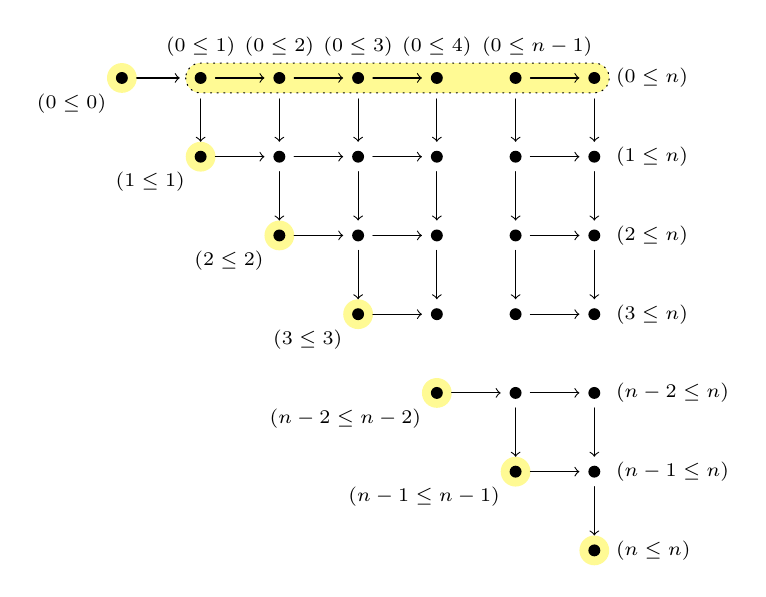
\begin{tikzpicture}[x=-1cm,y=-1cm,line cap=round]
			
			\draw[line width=2.5ex,yellow!42!white] (5,0) to (0,0);
			\fill[yellow!42!white] (6,0) circle (1.25ex);
			\fill[yellow!42!white] (5,1) circle (1.25ex);
			\fill[yellow!42!white] (4,2) circle (1.25ex);
			\fill[yellow!42!white] (3,3) circle (1.25ex);
			\fill[yellow!42!white] (2,4) circle (1.25ex);
			\fill[yellow!42!white] (1,5) circle (1.25ex);
			\fill[yellow!42!white] (0,6) circle (1.25ex);
			\fill (0,0) circle (0.5ex) coordinate (00);
			\fill (1,0) circle (0.5ex) coordinate (10);
			\fill (2,0) circle (0.5ex) coordinate (20);
			\fill (3,0) circle (0.5ex) coordinate (30);
			\fill (4,0) circle (0.5ex) coordinate (40);
			\fill (5,0) circle (0.5ex) coordinate (50);
			\fill (6,0) circle (0.5ex) coordinate (60);
			\fill (0,1) circle (0.5ex) coordinate (01);
			\fill (1,1) circle (0.5ex) coordinate (11);
			\fill (2,1) circle (0.5ex) coordinate (21);
			\fill (3,1) circle (0.5ex) coordinate (31);
			\fill (4,1) circle (0.5ex) coordinate (41);
			\fill (5,1) circle (0.5ex) coordinate (51);
			\fill (0,2) circle (0.5ex) coordinate (02);
			\fill (1,2) circle (0.5ex) coordinate (12);
			\fill (2,2) circle (0.5ex) coordinate (22);
			\fill (3,2) circle (0.5ex) coordinate (32);
			\fill (4,2) circle (0.5ex) coordinate (42);
			\fill (0,3) circle (0.5ex) coordinate (03);
			\fill (1,3) circle (0.5ex) coordinate (13);
			\fill (2,3) circle (0.5ex) coordinate (23);
			\fill (3,3) circle (0.5ex) coordinate (33);
			\fill (0,4) circle (0.5ex) coordinate (04);
			\fill (1,4) circle (0.5ex) coordinate (14);
			\fill (2,4) circle (0.5ex) coordinate (24);
			\fill (0,5) circle (0.5ex) coordinate (05);
			\fill (1,5) circle (0.5ex) coordinate (15);
			\fill (0,6) circle (0.5ex) coordinate (06);
			\node[below left=0.5ex] at (60) {\scriptsize $(0\leq 0)$};
			\node[above=1ex,shift={(0,0)}] at (50) {\scriptsize $(0\leq 1)$};
			\node[above=1ex,shift={(0,0)}] at (40) {\scriptsize $(0\leq 2)$};
			\node[above=1ex,shift={(0,0)}] at (30) {\scriptsize $(0\leq 3)$};
			\node[above=1ex,shift={(0,0)}] at (20) {\scriptsize $(0\leq 4)$};
			\node[above=1ex,shift={(-0.275,0)}] at (10) {\scriptsize $(0\leq n-1)$};
			\node[right=1ex] at (00) {\scriptsize $(0\leq n)$};
			\node[right=1ex] at (01) {\scriptsize $(1\leq n)$};
			\node[right=1ex] at (02) {\scriptsize $(2\leq n)$};
			\node[right=1ex] at (03) {\scriptsize $(3\leq n)$};
			\node[right=1ex] at (04) {\scriptsize $(n-2\leq n)$};
			\node[right=1ex] at (05) {\scriptsize $(n-1\leq n)$};
			\node[right=1ex] at (06) {\scriptsize $(n\leq n)$};
			\node[below left=0.5ex] at (51) {\scriptsize $(1\leq 1)$};
			\node[below left=0.5ex] at (42) {\scriptsize $(2\leq 2)$};
			\node[below left=0.5ex] at (33) {\scriptsize $(3\leq 3)$};
			\node[below left=0.5ex] at (24) {\scriptsize $(n-2\leq n-2)$};
			\node[below left=0.5ex] at (15) {\scriptsize $(n-1\leq n-1)$};
			\node at (4.5,0.5) {$\pushoutsign$};
			\node at (3.5,0.5) {$\pushoutsign$};
			\node at (2.5,0.5) {$\pushoutsign$};
			\node at (0.5,0.5) {$\pushoutsign$};
			\node at (3.5,1.5) {$\pushoutsign$};
			\node at (2.5,1.5) {$\pushoutsign$};
			\node at (0.5,1.5) {$\pushoutsign$};
			\node at (2.5,2.5) {$\pushoutsign$};
			\node at (0.5,2.5) {$\pushoutsign$};
			\node at (0.5,4.5) {$\pushoutsign$};
			\draw[-to,shorten <=1.25ex, shorten >=1.75ex] (60) to (50);
			\draw[-to,shorten <=1.25ex, shorten >=1.25ex] (50) to (40);
			\draw[-to,shorten <=1.25ex, shorten >=1.25ex] (40) to (30);
			\draw[-to,shorten <=1.25ex, shorten >=1.25ex] (30) to (20);
			\draw[-to,shorten <=1.25ex, shorten >=1.25ex] (10) to (00);
			\draw[-to,shorten <=1.25ex, shorten >=1.25ex] (51) to (41);
			\draw[-to,shorten <=1.25ex, shorten >=1.25ex] (41) to (31);
			\draw[-to,shorten <=1.25ex, shorten >=1.25ex] (31) to (21);
			\draw[-to,shorten <=1.25ex, shorten >=1.25ex] (11) to (01);
			\draw[-to,shorten <=1.25ex, shorten >=1.25ex] (42) to (32);
			\draw[-to,shorten <=1.25ex, shorten >=1.25ex] (32) to (22);
			\draw[-to,shorten <=1.25ex, shorten >=1.25ex] (12) to (02);
			\draw[-to,shorten <=1.25ex, shorten >=1.25ex] (33) to (23);
			\draw[-to,shorten <=1.25ex, shorten >=1.25ex] (13) to (03);
			\draw[-to,shorten <=1.25ex, shorten >=1.25ex] (24) to (14);
			\draw[-to,shorten <=1.25ex, shorten >=1.25ex] (14) to (04);
			\draw[-to,shorten <=1.25ex, shorten >=1.25ex] (15) to (05);
			\draw[-to,shorten <=1.75ex, shorten >=1.25ex] (50) to (51);
			\draw[-to,shorten <=1.75ex, shorten >=1.25ex] (40) to (41);
			\draw[-to,shorten <=1.75ex, shorten >=1.25ex] (30) to (31);
			\draw[-to,shorten <=1.75ex, shorten >=1.25ex] (20) to (21);
			\draw[-to,shorten <=1.75ex, shorten >=1.25ex] (10) to (11);
			\draw[-to,shorten <=1.75ex, shorten >=1.25ex] (00) to (01);
			\draw[-to,shorten <=1.25ex, shorten >=1.25ex] (41) to (42);
			\draw[-to,shorten <=1.25ex, shorten >=1.25ex] (31) to (32);
			\draw[-to,shorten <=1.25ex, shorten >=1.25ex] (21) to (22);
			\draw[-to,shorten <=1.25ex, shorten >=1.25ex] (11) to (12);
			\draw[-to,shorten <=1.25ex, shorten >=1.25ex] (01) to (02);
			\draw[-to,shorten <=1.25ex, shorten >=1.25ex] (32) to (33);
			\draw[-to,shorten <=1.25ex, shorten >=1.25ex] (22) to (23);
			\draw[-to,shorten <=1.25ex, shorten >=1.25ex] (12) to (13);
			\draw[-to,shorten <=1.25ex, shorten >=1.25ex] (02) to (03);
			\draw[-to,shorten <=1.25ex, shorten >=1.25ex] (14) to (15);
			\draw[-to,shorten <=1.25ex, shorten >=1.25ex] (04) to (05);
			\draw[-to,shorten <=1.25ex, shorten >=1.25ex] (05) to (06);
			\path (20) to node[pos=0.5] {$\dotso$} (10);
			\path (21) to node[pos=0.5] {$\dotso$} (11);
			\path (22) to node[pos=0.5] {$\dotso$} (12);
			\path (23) to node[pos=0.5] {$\dotso$} (13);
			\path (23) to node[pos=0.5,sloped] {$\dotso$} (24);
			\path (33) to node[pos=0.5,sloped] {$\dotso$} (24);
			\path (13) to node[pos=0.5,sloped] {$\dotso$} (14);
			\path (03) to node[pos=0.5,sloped] {$\dotso$} (04);
			\draw[dotted] (-5cm-1.25ex,0) to[out=270,in=180] (5,-1.25ex) to (0,-1.25ex) to[out=0,in=270] (1.25ex,0) to[out=90,in=0] (0,1.25ex) to (5,1.25ex) to[out=180,in=90] cycle;
		\end{tikzpicture}
	\end{center}
	Now \itememph{b} is equivalent to $F$ being left Kan extended from the \enquote{yellow} part. Together with \itememph{a}, this implies
	\begin{equation*}
		S_n(\Cc)\simeq \Fun\big([n-1],\Cc\big)
	\end{equation*}
	via restriction to the \enquote{dotted} part in the top row. Hence $S_n(\Cc)$ is stable again. Moreover, $\Fun(\Ar[n],\Cc)$ is clearly functorial both in $[n]$ and $\Cc$, and one checks that the full subcategories $S_n(\Cc)$ are preserved under the face and degeneracy maps in $\IDelta^\op$. Hence $S(C)\colon \IDelta^\op\morphism \Cat_\infty^\mathrm{st}$ is a simplicial stable $\infty$-category, and we get a functor
	\begin{equation*}
		S\colon \Cat_\infty^\mathrm{st}\morphism \cat{sCat}_\infty^\mathrm{st}\,.
	\end{equation*}
	Unravelling, we find that $S_0(\Cc)\simeq *$, $S_1(\Cc)\simeq \Cc$, and $S_1(\Cc)\simeq \Ar(\Cc)$. But we think of the typical element of $S_2(\Cc)$ as a diagram
	\begin{equation*}
		\begin{tikzcd}
			0\rar & a \rar\dar \drar[pushout]& b\dar\\
			& 0\rar & b/a\dar\\
			& & 0
		\end{tikzcd}
	\end{equation*}
	rather than an arrow $a\morphism b$. In this picture, the face maps $d_0,d_1,d_2\colon S_2(\Cc)\morphism S_1(\Cc)\simeq \Cc$ extract the objects $b/a$, $b$, and $a$, respectively.
	
	Also note that we have $\pi_0\left|\core S(\Cc)\right|=0$, since it is a general fact that $\pi_0X_0\morphism \pi_0\left|X\right|$ is surjective for all simplicial anima $X$ (see \itememph{*} in the proof of \cref{prop:CompletionOfMonoidsFullyFaithful}).
\end{con}
\begin{defi}\label{def:KTheoryOfStableInftyCategories}
	For a stable $\infty$-category $\Cc$, we define
	\begin{equation*}
		k(\Cc)\coloneqq \Omega \left|\core S(\Cc)\right|\,.
	\end{equation*}
	Since $\left|\core S(\Cc)\right|$ is connected, there's no need to specify a basepoint.
\end{defi}
\begin{lem}\label{lem:SkeletalInduction}
	For all stable $\infty$-categories $\Cc$, there is a canonical isomorphism
	\begin{equation*}
		K_0(\Cc)\simeq \pi_0\big(k(\Cc)\big)\simeq \pi_1\big(\left|\core(\Cc)\right|\big)\,.
	\end{equation*}
\end{lem}
\begin{proof}
	The second isomorphism is clear as the loop functor shifts homotopy groups down. Hence it suffices to show $K_0(\Cc)\simeq \pi_1(\left|\core(\Cc)\right|)$. This will be done using skeletal induction. We didn't talk about how this works for simplicial anima, so this proof also serves as a demonstration of the technique (although we will actually do skeletal induction for semi-simplicial anima, since that's somewhat easier and sufficient for our purposes).
	
	Let $\IDelta_\mathrm{inj}\subseteq\IDelta$ be the subcategory spanned by the injective maps. It is \emph{wide}, i.e.\ contains all objects, but obviously not full. Using the criterion from \cref{thm:JoyalQuillenThmA}\itememph{b}, one easily checks that $\IDelta^\op_\mathrm{inj}\subseteq \IDelta^\op$ is cofinal. So instead of the realisation $|X|\simeq \colimit_{\IDelta^\op}X$ of some simplicial anima $X$, we may consider the colimit over $\IDelta^\op_\mathrm{inj}$ of its restriction. Somewhat abusingly, we won't distinguish between $X$ and its restriction to $\IDelta^\op_\mathrm{inj}$. 
	
	Next, let's define the skeletal filtration on $X$. For all $n\geq 0$, let $i_n$ denote the inclusion $\IDelta_{\mathrm{inj},\leq n}\subseteq \IDelta_\mathrm{inj}^\op$. Then put
	\begin{equation*}
		\sk_n X\coloneqq \Lan_{i_n} i_n^*X\,.
	\end{equation*}
	Using the explicit fromulas from \cref{thm:KanExtension}, one unravels 
	\begin{equation*}
		(\sk_nX)_k\simeq \begin{cases*}
			X_k & if $k\leq n$\\
			\emptyset & if $k> n$
		\end{cases*}\,.
	\end{equation*}
	The $\sk_nX$ assemble into a functor $\sk X\colon \IN\morphism \Fun(\IDelta_\mathrm{inj}^\op,\An)$ with colimit $X$ (which is clear from the above description and the fact that colimits in functor categories are pointwise).
	
	Now consider
	\begin{equation*}
		\snake{\Delta}^n =\Hom_{\IDelta^\op_\mathrm{inj}}\big(-,[n]\big)\quad\text{and}\quad \partial \snake{\Delta}^n=\sk_{n-1}\snake{\Delta}^n
	\end{equation*}
	in $\Fun(\IDelta^\op_\mathrm{inj},\An)$, the \enquote{semi-simplicial $n$-simplex} and its \enquote{boundary}. Note that $\snake{\Delta}^n$ and $\partial \snake{\Delta}^n$ are \emph{not} the restrictions of $\Delta^n$ and $\partial \Delta^n$ to $\IDelta_\mathrm{inj}^\op$! However, $\Delta^n$ and $\partial \Delta^n$ are the left Kan extensions of $\snake{\Delta}^n$ and $\partial \snake{\Delta}^n$  along $\IDelta^\op_\mathrm{inj}\subseteq \IDelta^\op$ by \cref{cor:f_!:PC->PD}. Hence
	\begin{equation*}
	 	|\snake{\Delta}^n|\simeq |\Delta^n|\simeq *\quad\text{and}\quad |\partial\snake{\Delta}^n|\simeq |\partial\Delta^n|\simeq \IS^{n-1}\,,
	\end{equation*}
 	where we use that $\colimit_{\IDelta_{\mathrm{inj}}^\op}$ and $\colimit_{\IDelta^\op}$ are the left Kan extension functors along $\IDelta_\mathrm{inj}^\op\morphism *$ and $\IDelta^\op\morphism *$, respectively, and left Kan extension composes. 
	
	By direct inspection there are pushouts
	\begin{equation}\label{eq:SkeletalInduction0}
		\begin{tikzcd}
			\partial\snake{\Delta}^{n+1}\times \const X_{n+1}\dar\rar\drar[pushout] & \sk_n X\dar\\
			\snake{\Delta}^{n+1}\times \const X_{n+1}\rar & \sk_{n+1}X
		\end{tikzcd}
	\end{equation}
	for all $n\geq 0$ (just write out the definitions and everything will be trivial in each degree). Taking realisations everywhere gives pushouts
	\begin{equation}\label{eq:SkeletalInduction}
		\begin{tikzcd}
			\IS^n\times X_{n+1}\dar\rar\drar[pushout] & {\left|\sk_n X\right|}\dar\\
			X_{n+1}\rar & {\left|\sk_{n+1}X\right|}
		\end{tikzcd}
	\end{equation}
	for all $n\geq 0$. But be aware of \cref{warn:SemisimplicialRealisationDoesntCommuteWithProducts} below!
	
	
	Now apply \cref{eq:SkeletalInduction} to $X\simeq \core S(\Cc)$ in the case $n=0$. We know $S_1(\Cc)\simeq \Cc$ and hence $\IS^0\times \core S_1(\Cc)\simeq \core(\Cc)\sqcup \core(\Cc)$. Thus the pushout diagram in question appears as
	\begin{equation*}
		\begin{tikzcd}
			\core(\Cc)\sqcup\core(\Cc)\dar\rar\drar[pushout] & {\left|\sk_0 \core S(\Cc)\right|}\dar\\
			\core(\Cc) \rar & {\left|\sk_{1}\core S(\Cc)\right|}
		\end{tikzcd}
	\end{equation*}
	We also know $S_0(\Cc)\simeq *$, hence $\sk_0\core S(\Cc)\simeq \snake{\Delta}^0$. Plugging this into the pushout above and playing a bit around with it then shows $\left|\sk_{1}\core S(\Cc)\right|\simeq \Sigma(\core(\Cc)\sqcup *)\simeq \Sigma(\core(\Cc)_+)$. Hence $\Omega \left|\sk_{1}\core S(\Cc)\right|\simeq \Omega\Sigma (\core(\Cc)_+)\simeq \Free^\Grp(\core(\Cc))$ by \cref{prop:FreeGroups}. Therefore
	\begin{equation*}
		\pi_1\left|\sk_{1}\core S(\Cc)\right|= \pi_0\Free^\Grp\big(\core(\Cc)\big)=\Free^{\Grp(\Set)}\big(\pi_0\core(\Cc)\big)
	\end{equation*}
	is the free ordinary group on the set $\pi_0\core(\Cc)$.
	
	Next, we apply \cref{eq:SkeletalInduction} to $X\simeq \core S(\Cc)$ in the case $n=1$. Plugging in what we know so far, the pushout in question appears as
	\begin{equation*}
		\begin{tikzcd}
			\IS^1\times \core S_2(\Cc)\dar\rar\drar[pushout] & \Sigma\big(\core(\Cc)\sqcup *\big)\dar\\
			\core S_2(\Cc)\rar & {\left|\sk_2\core S(\Cc)\right|}
		\end{tikzcd}
	\end{equation*}
	This enables us to compute $\pi_1\left|\sk_2\core S(\Cc)\right|$ using the Seifert--van Kampen theorem (\cite[Theorem~1.20]{Hatcher}). But note that $\core S_2(\Cc)$ isn't necessarily connected; rather, each equivalence class in $S_2(\Cc)$ defines a connected component. So in order to use Seifert--van Kampen in its usual formulation, we have to decompose $\core S_2(\Cc)\simeq \coprod_{s}(\core S_2(\Cc))_s$ into pathcomponents and then iteratively form the pushout along $\IS^1\times (\core S_2(\Cc))_s\morphism (\core S_2(\Cc))_s$ (where the \enquote{number} of iterations can be any ordinal).
	
	So choose an element $s\in \core S_2(\Cc)$, which we may think of as a cofibre sequence
	\begin{equation*}
		s=(a\morphism b\morphism b/a)
	\end{equation*}
	in $\Cc$, and let's unravel what the top row map does on fundamental groups. We know $\pi_1\Sigma(\core(\Cc)\sqcup *)=\Free^{\Grp(\Set)}(\pi_0\core(\Cc))$, $\pi_1(\IS^1)=\IZ$, and that $\pi_1$ commutes with products. We claim that the ensuing map
	\begin{equation*}
		\IZ\times \pi_1\big(\core S_2(\Cc),s\big)\morphism \Free^{\Grp(\Set)}\big(\pi_0\core(\Cc)\big)
	\end{equation*}
	sends $(1,e)\mapsto a\cdot b^{-1}\cdot b/a$  and $(0,\gamma)\mapsto e$ for all $\gamma\in \pi_1(\core S_2(\Cc),s)$, where $e$ denotes the respective neutral elements. Indeed, $(1,e)$ corresponds to walking once around the perimeter of $\IS^1\simeq |\partial\snake{\Delta}^1|$ and taking boundary maps, which are given by $d_2(s)\simeq a$, $d_1(s)\simeq b$, and $d_0(s)\simeq b/a$ in that order (see the end of \cref{con:SConstruction}). The argument for $(0,\gamma)$ is similar. To make all of this really precise,  we would have to unravel what the top row  map $\partial\snake{\Delta}^{n+1}\times \const X_{n+1}\morphism \sk_n X$ from \cref{eq:SkeletalInduction0} does, but let's not get into the details there.
	
	So taking the pushout 
	\begin{equation*}
		\begin{tikzcd}
			\IZ\times \pi_1\big(\core S_2(\Cc),s\big)\dar["\pr_2"]\drar[pushout]\rar &\Free^{\Grp(\Set)}\big(\pi_0\core(\Cc)\big)\dar[dashed]\\
			\pi_1\big(\core S_2(\Cc),s\big) \rar[dashed] & \boldsymbol{?}
		\end{tikzcd}
	\end{equation*}
	in $\Grp(\Set)$ (which is what the Seifert--van Kampen theorem does) precisely enforces the relation $[b]=[b/a]\cdot [a]$ in the free group $\Free^{\Grp(\Set)}(\pi_0\core(\Cc))$. Doing this for all cofibre sequences in $\Cc$ thus provides an isomorphism
	\begin{equation*}
		K_0(\Cc)\simeq \pi_1\big(\left|\sk_2\core S_2(\Cc)\right|\big)
	\end{equation*}
	(note in particular that $a\morphism a\oplus c\morphism c$ is always a fibre sequence, hence $[a\oplus c]=[a]\cdot [c]$, and then by swapping $a$ and $c$ also $[a\oplus c]=[c]\cdot [a]$). Thus we are almost done and it only remains to show $\pi_1(|\sk_2\core S (\Cc)|)=\pi_1(\left|\core(\Cc)\right|)$. But it follows from \cref{eq:SkeletalInduction} and the Seifert--van Kampen theorem again that the fundamental group doesn't change anymore in the higher skeleta (because $\pi_1(\IS^n)=0$ for $n\geq 2$). Thus, as $\pi_1$ commutes with sequential colimits by \cref{lem:piPreservesSequentialColimits},
	\begin{align*}
		\pi_1\big(\left|\core(\Cc)\right|\big)&=\pi_1\left(\colimit_{n\in\IN}\left|\sk_n\core S_2(\Cc)\right|\right)\\
		&=\colimit_{n\in\IN}\pi_1\big(\left|\sk_2\core S_2(\Cc)\right|\big)\\
		&=\pi_1\big(\left|\sk_2\core S_2(\Cc)\right|\big)\,.\tag*{\qedhere}
	\end{align*}
\end{proof}
\begin{smallwarn}\label{warn:SemisimplicialRealisationDoesntCommuteWithProducts}
	In contrast to the realisation of simplicial anima (see \cref{prop:RealisationCommutesWithFiniteProducts}), the realisation functor
	\begin{equation*}
		|\blank|\simeq \colimit_{\IDelta_\mathrm{inj}^\op}\colon \Fun(\IDelta_\mathrm{inj}^\op,\An)\morphism \An
	\end{equation*}
	for semi-simplicial anima doesn't commute with finite products in general. For example $\snake{\Delta}^0\times \snake{\Delta}^1\simeq\snake{\Delta}^0\sqcup \snake{\Delta}^1$, so $|\snake{\Delta}^0\times \snake{\Delta}^1|\simeq|\snake{\Delta}^0|\sqcup |\snake{\Delta}^1|$. But it does if one object is constant, since both $|X\times \const -|\colon \An\morphism \An$ and $|X|\times -\colon \An\morphism \An$ preserve colimits and agree on $*\in\An$, hence they must agree by \cref{thm:ColimitPreservingRepresentable}.
\end{smallwarn}
\refstepcounter{smallerdummy}
\numpar*{\thesmallerdummy. Edgewise Subdivision}\label{par:edgewiseSubdivision}
Let's give another construction of $k(\Cc)$ using the Quillen $Q$-construction from \cref{par:QuillenQConstruction}. To get a relation between the $Q$- and the $S$-construction, consider
\begin{align*}
	\IDelta^\op&\morphism \IDelta^\op\\
	[n]&\longmapsto [n]\star [n]^\op\,.
\end{align*}
It induces a functor $(-)^\mathrm{esd}\colon \cat{sAn}\morphism \cat{sAn}$, called \emph{edgewise subdivision}. For example, by \cref{lem:NrTwAr}, \begin{equation*}
	\N^r(\Cc)^\mathrm{esd}\simeq \N^r\big(\TwAr(\Cc^\op)\big)
\end{equation*}
holds for all $\infty$-categories $\Cc$. Moreover, we have
\begin{equation*}
	|X|\simeq |X^\mathrm{esd}|
\end{equation*}
for all simplicial anima $X$. Indeed, both sides are colimit preserving functors $\cat{sAn}\morphism \An$, hence it suffices to check that they coincide on simplices by \cref{thm:ColimitPreservingRepresentable}. Clearly $|\Delta^n|\simeq *$. To get the same for $(\Delta^n)^\mathrm{esd}$, we use $\N^r([n])\simeq \Delta^n$ (see before \cref{thmdef:RezkNerve}) and thus $(\Delta^n)^\mathrm{esd}\simeq \N^r(\TwAr([n]^\op))$ by the formula above. But $\TwAr([n]^\op)$ has an initial object, hence its realisation is contractible too.

Abstractly, $[n]^\op\star[n]= [2n+1]$. But rather than as the poset $(0<1<\dotsb<2n+1)$, we think of $[n]^\op\star[n]$ as the poset
\begin{equation*}
	(0_\ell < 1_\ell < \dotsb < n_\ell < n_r < (n-1)_r < \dotsb < 0_r)\,,
\end{equation*}
where the indices $(-)_\ell$ and $(-)_r$ indicate the \enquote{left} and \enquote{right} part, corresponding to $[n]$ and $[n]^\op$ respectively.

\begin{prop}\label{prop:QvsS}
	The map $\TwAr\big([n]^\op)\morphism \Ar([n]\star [n]^\op)$ sending $(i\leq j)$ to $(i_\ell\leq j_r)$
	induces an equivalence
	\begin{equation*}
		S(\Cc)^\mathrm{esd}\isomorphism Q(\Cc)
	\end{equation*}
	for any stable $\infty$-category $\Cc$. In particular, $k(\Cc)\simeq \Omega\left|\Span(\Cc)\right|$, where we put $\Span(\Cc)\simeq \asscat(\core Q(\Cc))$, as defined in \cref{propdef:SpanQ}.
\end{prop}
\begin{proof}[Proof sketch]
	It's easy to check that $\TwAr\big([n]^\op)\morphism \Ar([n]\star [n]^\op)$ defines a map of simplicial posets and that the induced map upon taking $\Fun(-,\Cc)$ restricts to a map $S(\Cc)^\mathrm{esd}\morphism Q(\Cc)$, as required.
	
	To show that this map is indeed an equivalence, we draw a picture in the case $n=2$, that is, a picture of $\Ar([2]\star [2]^\op)\simeq \Ar([5])$:
	\begin{center}
		\begin{tikzpicture}[x=-1cm,y=-1cm,line cap=round,line join=round]
			%\scriptsize
			\draw[line width=2.5ex,yellow!42!white] (1,0) to (3,0) to (3,2);
			\draw[line width=2.5ex,yellow!42!white] (2,0) to (2,1) to (3,1);
			\fill[FabiansPink!42!white] (6,0) circle (1.25ex);
			\fill[FabiansPink!42!white] (5,1) circle (1.25ex);
			\fill[FabiansPink!42!white] (4,2) circle (1.25ex);
			\fill[FabiansPurple!42!white] (3,3) circle (1.25ex);
			\fill[FabiansPurple!42!white] (2,4) circle (1.25ex);
			\fill[FabiansPurple!42!white] (1,5) circle (1.25ex);
			\fill (1,0) circle (0.5ex) coordinate (10);
			\fill (2,0) circle (0.5ex) coordinate (20);
			\fill (3,0) circle (0.5ex) coordinate (30);
			\fill (4,0) circle (0.5ex) coordinate (40);
			\fill (5,0) circle (0.5ex) coordinate (50);
			\fill (6,0) circle (0.5ex) coordinate (60);
			\fill (1,1) circle (0.5ex) coordinate (11);
			\fill (2,1) circle (0.5ex) coordinate (21);
			\fill (3,1) circle (0.5ex) coordinate (31);
			\fill (4,1) circle (0.5ex) coordinate (41);
			\fill (5,1) circle (0.5ex) coordinate (51);
			\fill (1,2) circle (0.5ex) coordinate (12);
			\fill (2,2) circle (0.5ex) coordinate (22);
			\fill (3,2) circle (0.5ex) coordinate (32);
			\fill (4,2) circle (0.5ex) coordinate (42);
			\fill (1,3) circle (0.5ex) coordinate (13);
			\fill (2,3) circle (0.5ex) coordinate (23);
			\fill (3,3) circle (0.5ex) coordinate (33);
			\fill (1,4) circle (0.5ex) coordinate (14);
			\fill (2,4) circle (0.5ex) coordinate (24);
			\fill (1,5) circle (0.5ex) coordinate (15);
			
			\node[below left=0.5ex] at (60) {\scriptsize $(0_\ell\leq 0_\ell)$};
			\node[above=1ex,shift={(0.375,0)}] at (50) {\scriptsize $(0_\ell\leq 1_\ell)$};
			\node[above=1ex,shift={(0.125,0)}] at (40) {\scriptsize $(0_\ell\leq 2_\ell)$};
			\node[above=1ex,shift={(-0.125,0)}] at (30) {\scriptsize $(0_\ell\leq 2_r)$};
			\node[above=1ex,shift={(-0.375,0)}] at (20) {\scriptsize $(0_\ell\leq 1_r)$};
			\node[right=1ex] at (10) {\scriptsize $(0_\ell\leq 0_r)$};
			\node[right=1ex] at (11) {\scriptsize $(1_\ell\leq 0_r)$};
			\node[right=1ex] at (12) {\scriptsize $(2_\ell\leq 0_r)$};
			\node[right=1ex] at (13) {\scriptsize $(2_r\leq 0_r)$};
			\node[right=1ex] at (14) {\scriptsize $(1_r\leq 0_r)$};
			\node[below=1ex] at (15) {\scriptsize $(0_r\leq 0_r)$};
			\node[below left=0.5ex] at (51) {\scriptsize $(1_\ell\leq 1_\ell)$};
			\node[below left=0.5ex] at (42) {\scriptsize $(2_\ell\leq 2_\ell)$};
			\node[below left=0.5ex] at (33) {\scriptsize $(2_r\leq 2_r)$};
			\node[below left=0.5ex] at (24) {\scriptsize $(1_r\leq 1_r)$};
			\draw[-to,shorten <=1.25ex, shorten >=1.25ex] (60) to (50);
			\draw[-to,shorten <=1.25ex, shorten >=1.25ex] (50) to (40);
			\draw[-to,shorten <=1.25ex, shorten >=1.25ex] (40) to (30);
			\draw[-to,shorten <=1.25ex, shorten >=1.25ex] (30) to (20);
			\draw[-to,shorten <=1.25ex, shorten >=1.25ex] (51) to (41);
			\draw[-to,shorten <=1.25ex, shorten >=1.25ex] (41) to (31);
			\draw[-to,shorten <=1.25ex, shorten >=1.25ex] (31) to (21);
			\draw[-to,shorten <=1.25ex, shorten >=1.25ex] (42) to (32);
			\draw[-to,shorten <=1.25ex, shorten >=1.25ex] (32) to (22);
			\draw[-to,shorten <=1.25ex, shorten >=1.25ex] (33) to (23);
			\draw[-to,shorten <=1.25ex, shorten >=1.25ex] (24) to (14);
			\draw[-to,shorten <=1.75ex, shorten >=1.25ex] (50) to (51);
			\draw[-to,shorten <=1.75ex, shorten >=1.25ex] (40) to (41);
			\draw[-to,shorten <=1.75ex, shorten >=1.25ex] (30) to (31);
			\draw[-to,shorten <=1.75ex, shorten >=1.25ex] (20) to (21);
			\draw[-to,shorten <=1.75ex, shorten >=1.25ex] (10) to (11);
			\draw[-to,shorten <=1.25ex, shorten >=1.25ex] (41) to (42);
			\draw[-to,shorten <=1.25ex, shorten >=1.25ex] (31) to (32);
			\draw[-to,shorten <=1.25ex, shorten >=1.25ex] (21) to (22);
			\draw[-to,shorten <=1.25ex, shorten >=1.25ex] (11) to (12);
			\draw[-to,shorten <=1.25ex, shorten >=1.25ex] (32) to (33);
			\draw[-to,shorten <=1.25ex, shorten >=1.25ex] (22) to (23);
			\draw[-to,shorten <=1.25ex, shorten >=1.25ex] (12) to (13);
			\draw[-to,shorten <=1.25ex, shorten >=1.25ex] (14) to (15);
			\draw[-to,shorten <=1.25ex, shorten >=1.25ex] (20) to (10);
			\draw[-to,shorten <=1.25ex, shorten >=1.25ex] (21) to (11);
			\draw[-to,shorten <=1.25ex, shorten >=1.25ex] (22) to (12);
			\draw[-to,shorten <=1.25ex, shorten >=1.25ex] (23) to (13);
			\draw[-to,shorten <=1.25ex, shorten >=1.25ex] (23) to (24);
			\draw[-to,shorten <=1.25ex, shorten >=1.25ex] (13) to (14);
			\coordinate[shift={(225:1.25ex)}] (A) at (60);
			\coordinate[shift={(225:1.25ex)}] (B) at (42);
			\coordinate[shift={(270:1.25ex)}] (C) at (42);
			\coordinate[shift={(270:1.25ex)}] (D) at (32);
			\coordinate[shift={(315:1.25ex)}] (E) at (32);
			\coordinate[shift={(315:1.25ex)}] (F) at (10);
			\coordinate[shift={(22.5:1.25ex)}] (G) at (10);
			\coordinate[shift={(90:1.25ex)}] (H) at (10);
			\coordinate[shift={(90:1.25ex)}] (I) at (60);
			\coordinate[shift={(157.5:1.25ex)}] (J) at (60);
			\draw[dotted] (A) to (B) to[out=-45,in=180] (C) to (D) to[out=0,in=225] (E) to (F) to[out=45,in=292.5] (G) to[out=112.5,in=0] (H) to (I) to[out=180,in=67.5] (J) to[out=247.5,in=135] cycle;
		\end{tikzpicture}
	\end{center}
	We let $I_n$ denote the image of $\TwAr([n]^\op)\morphism \Ar([n]\star[n]^\op)$. This is the yellow part in the picture. Also let $\Delta_n^\ell$ and $\Delta_n^r$ be the subposets spanned by $\{(0_\ell\leq 0_\ell),\dotsc,(n_\ell\leq n_\ell)\}$ and $\{(n_r,n_r),\dotsc,(0_r,0_r)\}$, respectively. In the picture these are coloured pink and purple. Finally, let $J_n$ be the subposet spanned by $\left\{(i_\ell\leq j_\ell), (i_\ell\leq j_r)\st i\leq j\right\}$. This is the dotted part in the picture.
	
	By definition, an element lies in $S_{2n+1}(\Cc)$ iff all squares go to pushouts/pullbacks in the stable $\infty$-category $\Cc$. Moreover, $Q_n(\Cc)\subseteq \Fun(I_n,\Cc)$ is the full sub-$\infty$-category of those functors that send all squares in $I_n$ to pushouts/pullbacks. Now consider the composition
	\begin{equation*}
		\begin{tikzcd}
			\Fun(I_n,\Cc)\dar["\Lan"']\ar[rr,dashed] & &\Fun\big(\Ar([n]\star [n]^\op),\Cc\big)\\
			 \Fun(I_n\cup\Delta_n^\ell,\Cc)\rar["\Ran"] & \Fun(I_n\cup\Delta^n\cup\Delta_n^r,\Cc)\rar["\Ran"] & \Fun(J_n\cup\Delta_n^r,\Cc)\uar["\Lan"']
		\end{tikzcd}
	\end{equation*}
	(where \enquote{$\cup$} always means that we take the full subposet spanned by the union). That is, we start with the yellow part, left-Kan extend to the pink part, right-Kan extend to the purple part, right-Kan extend to the dotted part, and the left-Kan extend to all of $\Ar([n]\star [n]^\op)$. All of these Kan extensions are along fully faithful embeddings of subposets, hence fully faithful by \cref{cor:FullyFaithfulKanExtension}. Breaking up each of the Kan extensions into a sequence of Kan extensions by adding one vertex at a time, and using the formulas from \cref{thm:KanExtension}, we verify that the essential image of $Q_n\subseteq \Fun(I_n,\Cc)$ is precisely $S_{2n+1}(\Cc)\subseteq \Fun(\Ar([n]\star [n]^\op),\Cc)$, which is what we want.
	
	For the \enquote{in particular}, note that $\left|\core S(\Cc)\right|\simeq |\core S(\Cc)^\mathrm{esd}|\simeq \left|\core Q(\Cc)\right|$ holds by \labelcref{par:edgewiseSubdivision} and what we've shown so far, and $\left|\core Q(\Cc)\right|\simeq \left|\Span(\Cc)\right|$ follows from \cref{rem:Realisation}.
\end{proof}
\subsection{The Resolution Theorem}
\cref{prop:QvsS} allows us to define a map $\core(\Cc)\morphism k(\Cc)$ via
\begin{equation*}
	\core(\Cc)\simeq \Hom_{\Span(\Cc)}(0,0)\morphism \Hom_{\left|\Span(\Cc)\right|}(0,0)\simeq \Omega \left|\Span(\Cc)\right|
\end{equation*}
(the equivalence on the left follows from \cref{eq:asscat2} applied to $\Span(\Cc)\simeq \asscat(\core Q(\Cc))$ and some playing around with the pullback involved). This morphism is clearly natural in $\Cc$, hence it defines a natural transformation $\core\Rightarrow k$ in $\Fun(\Cat_\infty^\mathrm{st},\An)$. But both functors preserve finite products (because they are built from right adjoints, except for the realisation $|\blank|$, but this also preserves finite products by \cref{prop:RealisationCommutesWithFiniteProducts}). Hence it lifts canonically to a natural transformation
\begin{equation*}
	(\core \Longrightarrow k)\colon \Cat_\infty^\mathrm{st}\morphism \CMon(\An)
\end{equation*}
by \cref{thm:CMonCGrpAdjunctions} and the following observation:
\begin{obs}\label{obs:CatStSemiAdditive}
	$\Cat_\infty^\mathrm{st}$ is semi-additive \embrace{and the same is true for $\Cat_\infty^\sqcup$, $\Cat_\infty^\times$, and $\Cat_\infty^\mathrm{semi\mhyph add}$}.
\end{obs}
\begin{proof}[Proof sketch]
	Evidently, $\Cat_\infty^\mathrm{st}$ inherits products from $\Cat_\infty$, and the zero category $0\in \Cat_\infty^\mathrm{st}$ is a zero object. Next, recall \cref{prop:CocartesianMonoidalStructure}, which associates to every $\infty$-category $\Cc$ an $\infty$-operad $\Cc^\sqcup\morphism \IGamma^\op$. If you stare at the construction, you'll find it is clearly functorial in $\Cc$, hence we get a functor
	\begin{equation*}
		(-)^\sqcup\colon \Cat_\infty\morphism \Op_\infty\,.
	\end{equation*}
	But if $\Cc$ is stable, then it has finite coproducts and thus $\Cc^\sqcup\morphism \IGamma^\op$ is a symmetric monoidal $\infty$-category. Moreover, any map $F\colon \Cc\morphism\Dd$ in $\Cat_\infty^\mathrm{st}$ preserves finite coproducts, so its image  $F^\sqcup\colon \Cc^\sqcup\morphism\Dd^\sqcup$ is strongly monoidal. Hence $(-)^\sqcup$ restricts to a functor
	\begin{equation*}
		(-)^\oplus\colon \Cat_\infty^\mathrm{st}\morphism\CMon(\Cat_\infty)\,.
	\end{equation*}
	From this, we can extract functors $\oplus_\Cc\colon \Cc\times \Cc\morphism \Cc$ in $\Cat_\infty^\mathrm{st}$ which assemble into a natural transformation $\oplus\colon \Delta\Rightarrow \id$ in $\Fun(\Cat_\infty^\mathrm{st},\Cat_\infty^\mathrm{st})$ with the properties from  \cref{lem:SemiAddCriterion}. Hence that lemma implies that $\Cat_\infty^\mathrm{st}$ is semi-additive. The other cases are similar.
\end{proof}
\refstepcounter{smallerdummy}
\numpar*{\thesmallerdummy}\label{par:ProjRKDperRComparisonMap}
So for all stable $\infty$-categories $\Cc$ we get a map of $\IE_\infty$-monoids $\core(\Cc)\morphism k(\Cc)$. But $k(\Cc)$ is an $\IE_\infty$-group (because $\pi_0(k(\Cc))=K_0(\Cc)$ is an ordinary abelian group), hence this map factors over an $\IE_\infty$-group map
\begin{equation*}
	\core(\Cc)^\inftygrp\morphism k(\Cc)\,.
\end{equation*}
In particular, via $\Proj(R)\subseteq \core\Dd^\perf(R)$ this gives a map
\begin{equation*}
	k(R)\simeq \Proj(R)^\inftygrp\morphism \big(\core \Dd^\perf(R)\big)^\inftygrp \morphism k\big(\Dd^\perf(R)\big)\,.
\end{equation*}
And this map turns out to be an equivalence! Thereby we've reduced algebraic $K$-theory of rings, as constructed in \cref{def:AlgebraicKTheory}, to the more general construction from \cref{def:KTheoryOfStableInftyCategories}.

In fact, the equivalence $\Proj(R)^\inftygrp\simeq k(\Dd^\perf(R))$ can be proved in much more generality, but this needs a bit more terminology.
\numpar{Weight Structures*}\label{par:WeightStructure}
We didn't introduce this in the lecture, but here's what Fabian told the audience in his talk in Regensburg. A \emph{weight structure} on a stable $\infty$-category consists of two full sub-$\infty$-categories $\Cc_{\leq 0},\Cc_{\geq 0}\subseteq \Cc$ subject to the following conditions:
\begin{alphanumerate}
	\item $\Cc_{\geq 0}$ is closed under pushouts, $\Cc_{\leq 0}$ is closed under pullbacks, and both are closed under retracts.
	\item If $x\in \Cc_{\leq 0}$ and $y\in \Cc_{\geq 0}$, then the spectrum $\hom_\Cc(x,y)$ is connective (i.e.\ its homotopy groups vanish in negative degrees).
	\item For all $y\in \Cc$ there is a fibre sequence $x\morphism y\morphism z$ with $x\in \Cc_{\leq 0}$ and $z\in \Cc_{\geq 1}$. Here we put $\Cc_{\geq a}\coloneqq (\Cc_{\geq 0})[a]$ and $\Cc_{\leq b}\coloneqq (\Cc_{\leq 0})[b]$.
\end{alphanumerate}
We also put $\Cc_{[a,b]}\coloneqq \Cc_{\geq a}\cap \Cc_{\leq b}$, and $\Cc^\heartsuit\coloneqq \Cc_{[0,0]}=\Cc_{\geq 0}\cap \Cc_{\leq 0}$. A weight structure on $\Cc$ is called \emph{exhaustive} if
\begin{equation*}
	\Cc=\bigcup_{n\in\IN}\Cc_{[-n,n]}\,.
\end{equation*}
Fabian remarks that the notion of a weight structure is different from that of a $t$-structure (which you might know from \cite[Definition~\HAthm{1.2.1.4}]{HA}; we'll introduce it properly in \cref{par:tStructure}). For example, in a $t$-structure the roles of \enquote{$\leq$} and \enquote{$\geq$} in \itememph{c} would be swapped. You should think of $t$-structures as generalisations of \enquote{smart} truncation of chain complexes, whereas a weight structure behaves more like \enquote{stupid} truncation. In particular, the fibre sequence in $\Cc$ is highly non-canonical, whereas in a $t$-structure there's always a canonical choice using the truncation functors. Moreover, the heart of a $t$-structure is always an abelian category, whereas it need not even be a $1$-category for a weight structure.

Note that \itememph{a} implies that both $\Cc_{\geq 0}$ and $\Cc_{\leq 0}$ contain $0$, since it is a retract of everything (and both sub-$\infty$-categories are non-empty by \itememph{c}), and both are closed under finite direct sums. To acquaint myself a bit more with weight structures, let me also list the following further properties:
\begin{lem*}\label{lem*:MoreOnHearts}
	\begin{alphanumerate}
		\item An object $x\in \Cc$ lies in $\Cc_{\leq 0}$ iff $\hom_\Cc(x,y)$ is connective for all $y\in \Cc_{\geq 0}$. Similarly, $y\in \Cc$ lies in $\Cc_{\geq 0}$ iff $\hom_\Cc(x,y)$ is connective for all $x\in \Cc_{\leq 0}$.
		\item Both $\Cc_{\geq 0}$ and $\Cc_{\leq 0}$ are closed under extensions. That is, if the outer two terms in a fibre sequence lie in $\Cc_{\geq 0}$, then the same is true for the inner term, and likewise for  $\Cc_{\leq 0}$.
		\item $\Cc^\heartsuit$ is an additive $\infty$-category, and every fibre sequence $x\morphism y\morphism z$ in $\Cc$ splits if all of its terms lie in $\Cc^\heartsuit$.
	\end{alphanumerate}
\end{lem*}
\begin{proof*}
	For \itememph{a}, we only do the second case since the first one is analogous. The \enquote{only if} holds by assumption. So assume $y\in\Cc$ satisfies that $\hom_\Cc(x,y)$ is connective for all $x\in \Cc_{\leq 0}$. Apply \cref{par:WeightStructure}\itememph{c} to $y[1]$ to get a fibre sequence $x\morphism y\morphism z$ with $x\in \Cc_{\leq -1}$ and $z\in \Cc_{\geq 0}$. Then $\pi_0\hom_\Cc(x,y)=\pi_{-1}\hom_\Cc(x[1],y)=0$ by \cref{par:WeightStructure}\itememph{b}. Hence the long exact homotopy groups sequence associated to the fibre sequence $\hom_\Cc(z,y)\morphism \hom_\Cc(y,y)\morphism\hom_\Cc(x,y)$ in spectra becomes
	\begin{equation*}
		\dotso\morphism \pi_0\hom_\Cc(z,y)\morphism \pi_0\hom_\Cc(y,y)\morphism 0\,.
	\end{equation*}
	In particular, $\pi_0\hom_\Cc(z,y)\morphism \pi_0\hom_\Cc(y,y)$ is surjective. Choosing a preimage of $\id_y$ witnesses $y$ as a retract of $z$, hence $y\in \Cc_{\geq 0}$ because it is closed under retracts. This shows \itememph{a}. Part~\itememph{b} is an immediate consequence of \itememph{a} and the long exact homotopy groups sequence.
	
	It's clear that $\Cc^\heartsuit$ is contains $0$ and is closed under finite direct sums (in fact, under fibre sequences by \itememph{b}), hence it inherits additivity from $\Cc$. If $x\morphism y\morphism z$ is a fibre sequence in $\Cc$ whose terms lie in $\Cc^\heartsuit$, then $\hom_\Cc(z,x)\morphism \hom_\Cc(z,y)\morphism\hom_\Cc(z,z)$ is a fibre sequence in spectra. But all of its entries are connective, hence the long exact sequence of homotopy groups reads
	\begin{equation*}
		\dotso\morphism \pi_0\hom_\Cc(z,x)\morphism \pi_0\hom_\Cc(z,y)\morphism \pi_0\hom_\Cc(z,z)\morphism 0\,.
	\end{equation*}
	In particular, $\pi_0\hom_\Cc(z,y)\morphism \pi_0\hom_\Cc(z,z)$ is surjective, whence we get a split $z\morphism y$ by choosing a preimage of $\id_z$. Now consider the diagram
	\begin{equation*}
		\begin{tikzcd}
			0 \rar\dar\drar[dotted,pushout] & x \rar\dar\drar[pushout] & 0\dar\\
			z \rar & y\rar & z
		\end{tikzcd}
	\end{equation*}
	The right square is a pushout by assumption, and the outer rectangle is a pushout too since $z\morphism y\morphism z$ is equivalent to the identity on $z$. Hence the left square is a pushout as well, which establishes $y\simeq x\oplus z$.
\end{proof*}
The prime example of an exhaustive weight structure is $\Dd^\perf(R)$ for a ring $R$, with
\begin{equation*}
	\Dd^\perf(R)_{[a,b]}=\left\{C\in\Dd^\perf(R)\st\begin{tabular}{c}
		$C$ has a projective representative\\
		concentrated in degrees $[a,b]$
	\end{tabular}\right\}\,.
\end{equation*}
Note that this is stronger than heaving homology concentrated in degrees $[a,b]$! The heart of this weight structure is $\Dd^\perf(R)^\heartsuit\simeq\Proj(R)$.  With this, we can formulate a general version of the \enquote{resolution theorem}, also often called the \enquote{weight version of the theorem of the heart}.
\begin{thm}[Resolution theorem, Gillet--Waldhausen]\label{thm:Resolution}
	If $\Cc$ is a stable $\infty$-category equipped with an exhaustive weight structure, then composing $\core(\Cc^\heartsuit)^\inftygrp\morphism \core(\Cc)^\inftygrp$ with the map from \textup{\labelcref{par:ProjRKDperRComparisonMap}} induces an equivalence
	\begin{equation*}
		\core(\Cc^\heartsuit)^\inftygrp\morphism k(\Cc)\,.
	\end{equation*}
	In particular, $k(R)\simeq \Proj(R)^\inftygrp\simeq k(\Dd^\perf(R))$ for every ring $R$.
\end{thm}
We won't prove \cref{thm:Resolution}. But Fabian has promised he will sketch a new proof due to Wolfgang Steimle and himself in the official notes. In fact, they proved an even more general statement about \emph{Poincaré categories}, which Fabian will also introduce in his notes.
\section{\texorpdfstring{$K$}{K}-Theory as the Universal Additive Invariant}
\lecture[Lots of terminology named after Verdier. Recollements. The additivity theorem.\newline --- \emph{\enquote{Today there will be a definition that's longer than a page, and then a theorem that's longer than a page, and the theorem will essentially be trivial.}}]{2021-02-04}Our next goal is to analyse the functor $k\colon \Cat_\infty^\mathrm{st}\morphism \CGrp(\An)$, and in particular to prove the following result from \cite{BlumbergGepnerTabuada}:
\begin{thm}\label{thm:K=coreGrp}
	The inclusion $\Fun^{\grp}(\Cat_\infty^\mathrm{st},\CGrp(\An))\subseteq\Fun^\mathrm{add}(\Cat_\infty^\mathrm{st},\An)$ admits a left adjoint $(-)^\grp\simeq \Omega|\Span^{(-)}(-)|$, and 
	\begin{equation*}
		k\simeq \core^\grp\,.
	\end{equation*}
	In other words, $K$-theory is the initial grouplike functor under $\core\colon \Cat_\infty^\mathrm{st}\morphism \An$.
\end{thm}
The proof of \cref{thm:K=coreGrp} has to wait till page~\labelcpageref{page:ProofOfBlumbergGepnerTabuada}. Let's start with explaining all that new terminology in it, and to do that, we'll introduce even more.
\subsection{Verdier Sequences}
\begin{defi}\label{def:VerdierStuff}
	Let's define things named after Verdier:
	\begin{alphanumerate}
		\item A \emph{Verdier sequence} is a sequence $\Aa\morphism\Bb\morphism\Cc$ in $\Cat_\infty^\mathrm{st}$ that is both a fibre and a cofibre sequence. It is called \emph{left/right split} if both functors admit left/right adjoints, and \emph{split} if it is both left and right split (so all four possible adjoints exist).
		\item A functor $\Bb\morphism\Cc$ participating in a Verdier sequence as in \itememph{a} is called a \emph{Verdier projection}, and similarly $\Aa\morphism\Bb$ is called a \emph{Verdier injection}. A Verdier projection or injection is called \emph{left/right split} if the corresponding Verdier sequence has that property.
		\item A \emph{Verdier square} is a pullback square in $\Cat_\infty^\mathrm{st}$
		\begin{equation*}
			\begin{tikzcd}
				\Aa\dar\rar\drar[pullback] &\Bb\dar\\
				\Cc\rar & \Dd
			\end{tikzcd}
		\end{equation*}
		such that the vertical maps are Verdier projections. A Verdier square is called \emph{\embrace{left/right} split} if the Verdier projections have the respective property.
	\end{alphanumerate}
	Moreover, a functor $F \colon \Cat_\infty^\mathrm{st}\morphism \Ee$, where $\Ee$ has finite limits, is \emph{additive} or \emph{Verdier-localising} if $F(0)$ is a final object of $\Ee$ and $F$ takes split Verdier squares or all Verdier squares to pullback squares in $\Ee$. It is called \emph{Karoubi-localising} if it is Verdier-localising and takes dense inclusions to equivalences. The corresponding full sub-$\infty$-categories of $\Fun(\Cat_\infty^\mathrm{st},\Ee)$ are denoted
	\begin{equation*}
		\Fun^\mathrm{Kar}(\Cat_\infty^\mathrm{st},\Ee)\subseteq \Fun^\mathrm{Verd}(\Cat_\infty^\mathrm{st},\Ee)\subseteq \Fun^\add(\Catst,\Ee)\,.
	\end{equation*}
	Finally, an additive functor $F\colon\Catst\morphism \Ee$ is called \emph{grouplike} if it factors over $\CGrp(\Ee)$ (the factorisation is automatically canonical, see \cref{par:MoreOnVerdierSequences}\itememph{c}). The corresponding full sub-$\infty$-category is denoted
	\begin{equation*}
		\Fun^\grp(\Catst,\Ee)\subseteq \Fun^\add(\Catst,\Ee)\,.
	\end{equation*}
\end{defi}
\numpar{More on Verdier Sequences and Additive Functors}\label{par:MoreOnVerdierSequences}
Having introduced a plethora of new terminology in \cref{def:VerdierStuff}, some explanations are in order.
\begin{alphanumerate}
	\item The functor categories $\Fun(\Catst,\Ee)$ are usually not locally small. But we'll ignore set-theoretic issues in the following.
	\item In $\Cat_\infty^\mathrm{st}$ it is really a \emph{property} (rather than a structure) to be  a Verdier sequence: Given $\Aa\morphism \Bb\morphism\Cc$, an extension to
	\begin{equation*}
		\begin{tikzcd}
			\Aa\dar\rar &\Bb\dar\\
			0\rar & \Cc
		\end{tikzcd}
	\end{equation*}
	is unique (up to contractible choice) because $0\in \Fun(\Aa,\Cc)$ is initial and terminal.
	\item Because $\Cat_\infty^\mathrm{st}$ is semi-additive by \cref{obs:CatStSemiAdditive}, we obtain that
	\begin{equation*}
		\begin{tikzcd}
			\Aa\times \Cc\dar\rar\drar[pullback] &\Cc\dar\\
			\Aa\rar & 0
		\end{tikzcd}
	\end{equation*}
	is always a split Verdier square. Moreover, $\Cc\morphism \Cc\morphism 0$ is always a split Verdier sequence, and so is $\Cc\morphism \Aa\times \Cc\morphism \Aa$ in general. Hence additive functors preserve finite products. But then \cref{thm:CMonCGrpAdjunctions} implies that
	\begin{equation*}
		\Fun^\add(\Catst,\Ee)\simeq \Fun^\add\big(\Catst,\CMon(\Ee)\big)\simeq \CMon\big(\Fun^\add(\Catst,\Ee)\big)
	\end{equation*}
	for any $\infty$-category $\Ee$ with finite limits. Thus $\Fun^\grp(\Catst,\Ee)\subseteq \Fun^\add(\Catst,\Ee)$ as defined in \cref{def:VerdierStuff} makes sense, and also
	\begin{equation*}
		\Fun^\grp(\Catst,\Ee)\simeq \Fun^\add\big(\Catst,\CGrp(\Ee)\big)\simeq \CGrp\big(\Fun^\add(\Catst,\Ee)\big)\,.
	\end{equation*}
	Moreover, the arguments above show that $\Fun^\add(\Catst,\Ee)$ is semi-additive, and thus the same is true for $\Fun^\grp(\Catst,\Ee)$, $\Fun^\Verd(\Catst,\Ee)$, and $\Fun^\Kar(\Catst,\Ee)$. Finally, all of them are closed under limits in $\Fun(\Catst,\Ee)$.
	\item[\itememph{d^*}] If $F\colon \Catst\morphism \An$ is a grouplike additive functor, then $F(\Bb)\simeq F(A)\times F(\Cc)$ for every split Verdier sequence $\Aa\morphism \Bb\morphism \Cc$. Indeed, $F(\Aa)\morphism F(\Bb)\morphism F(\Cc)$ is a fibre sequence in $\An$, hence also in $\CGrp(\An)$. Either of the fully faithful adjoints $\Cc\morphism \Bb$ induces a split $F(\Cc)\morphism F(\Bb)$, so in particular, $\pi_0(F(\Bb))\morphism \pi_0(F(\Cc))$ is surjective. Hence the fibre $\fib(F(\Bb)\morphism F(\Cc))$ in $\Sp$ must be connective too, whence it coincides with the fibre $F(\Aa)$ taken in $\CGrp(\An)\simeq \Sp_{\geq 0}$. Now every fibre sequence in $\Sp$ with a split must actually \emph{be} split, using the same argument as in the proof of \cref{lem*:MoreOnHearts}\itememph{c}.
	\item[\itememph{e}] An example of a Verdier-localising but not grouplike functor is $\core\colon \Catst\morphism \An$. It is Verdier-localising simply because it takes arbitrary pullbacks (and not just Verdier squares) to pullbacks in $\An$.
	
	Here we should probably mention that $\Catst\subseteq \Cat_\infty$ is closed under pullbacks (and in fact, arbitrary finite limits). To see this, first note that $\Catst\subseteq\Cat_\infty^\mathrm{lex}$ has both adjoints by \cref{thm:SpLeftAdjoint} and the remark after it. Hence it suffices that $\Cat_\infty^\mathrm{lex}\subseteq \Cat_\infty$ is closed under pullbacks. But if we are given a pullback diagram in $\Cat_\infty$ such that both legs preserve finite limits, then any finite limit in the pullback can be computed componentwise (and in particular, exists if it exists componentwise).
\end{alphanumerate}
For even more facts about Verdier sequences, see \cite[Appendix~A]{9author2} and \labelcref{par:EvenMoreOnVerdierSequences} below.
\refstepcounter{smallerdummy}
\numpar*{\thesmallerdummy. Fibre Sequences in $\Catst$}\label{par:FibreSequencesInCatSt}
We can explicitly characterise fibre sequences in $\Catst$. Given an exact functor $p\colon \Bb\morphism \Cc$ between stable $\infty$-categories, the fibre $\fib(p)$ is the full subcategory
\begin{equation*}
	\fib(p)\simeq \left\{b\in \Bb\st p(b)\simeq 0\text{ in $\Cc$}\right\}\subseteq \Bb\,.
\end{equation*}
Since $p$ is exact, it's easy to show that $\fib(p)\subseteq \Bb$ is closed under finite direct sums and fibre/cofibre sequences, hence it is really a stable sub-$\infty$-category, and one immediately checks that $\fib(p)$ also satisfies the desired universal property.
\refstepcounter{smallerdummy}
\numpar*{\thesmallerdummy. Cofibre Sequences in $\Catst$}\label{par:CofibreSequencesInCatSt}
There's also an explicit description of cofibres in $\Catst$. Given an exact functor $f\colon \Aa\morphism\Bb$, by the \emph{essential image} of $f$ we mean the full sub-$\infty$-category of $\Bb$ spanned by all objects which are equivalent to some $f(a)$. Since $f$ is exact, the essential image is closed under finite direct sums, but not necessarily under fibres and cofibres, since there might be more morphisms in $\Bb$ than in $\Aa$. But there's always a smallest stable sub-$\infty$-category of $\Bb$ containing the essential image of $f$. In any case, we have
\begin{equation*}
	\cofib(f)\simeq \Bb/\Aa\coloneqq \Bb\big[\{\text{mod-$\Aa$ equivalences}\}^{-1}\big]\,,
\end{equation*}
where the mod-$\Aa$ equivalences are all those maps $\phi\colon x\morphism y$ whose fibre/cofibre is a retract of an object in the stable sub-$\infty$-category generated by the essential image of $f$. As $\fib(\phi)\simeq \cofib(\phi)[-1]$, it really suffices to assume that either one is such a retract.

In contrast to \itememph{c}, it's not so easy to show that $\cofib(f)\simeq \Bb/\Aa$ is a stable $\infty$-category again and that $\Bb\morphism \Bb/\Aa$ is an exact functor, so we'll postpone the proof until \cref{lem:VerdierQuotients}. But assuming this is true, it's easy to check that $\Bb/\Aa$ is indeed the correct cofibre: Let $\Cc$ be another stable $\infty$-category. By definition (see \cref{exm:Localisation}),
\begin{equation*}
	\Hom_{\Catst}(\Bb/\Aa,\Cc)\subseteq \Hom_{\Catst}(\Bb,\Cc)
\end{equation*}
is the collection of path components of functors that invert mod-$\Aa$ equivalences. But note that also
\begin{equation*}
	\Hom_{\Catst}\big(\cofib(f),\Cc\big)\simeq \Hom_{\Catst}(\Bb,\Cc)\times_{\Hom_{\Catst}(\Aa,\Cc)}\{0\}\subseteq \Hom_{\Catst}(\Bb,\Cc)
\end{equation*}
is also a collection of path components. This is because the zero functor is initial (and terminal) in $\Fun(\Aa,\Cc)$, hence its path component in $\Hom_{\Catst}(\Aa,\Cc)\subseteq \core \Fun(\Aa,\Cc)$ is a contractible anima, hence the inclusion of $\{0\}$ into it is an equivalence.

Therefore, it suffices to show $\Hom_{\Catst}(\Bb/\Aa,\Cc)$ and $\Hom_{\Catst}(\cofib(f),\Cc)$ comprise the same path components. But that's easy: Any exact functor $p\colon \Bb\morphism\Cc$ inverting the mod-$\Aa$ equivalences satisfies $p\circ f\simeq 0$, as $0\morphism p(a)$ is a mod-$\Aa$ equivalence for all $a\in \Aa$ Conversely, any exact $p\colon \Bb\morphism\Cc$ with $p\circ f\simeq 0$ also kills all retracts of the stable sub-$\infty$-category generated by the essential image of $f$. Hence it inverts mod-$\Aa$ equivalences.


\begin{thm}\label{thm:VerdierStuff}
	Let $F\colon \Aa\morphism\Bb$ be an exact functor of stable $\infty$-categories.
	\begin{alphanumerate}
		\item $F$ is a Verdier projection iff it is a localisation. In this case it automatically inverts precisely the mod-$\fib(F)$ equivalences.
		\item $F$ is a left/right split Verdier projection iff it admits a fully faithful left/right adjoint \embrace{i.e., iff it is a left/right Bousfield localisation}.
		\item $F$ is a Verdier inclusion iff it is fully faithful and its essential image is closed under retracts in $\Bb$.
		\item $F$ is a left/right split Verdier inclusion iff it is fully faithful and has a left/right adjoint.
	\end{alphanumerate}
	Furthermore, if 
	\begin{equation*}
		\begin{tikzcd}
			\Aa\rar["f"'] & \Bb\rar["p"']\lar[dashed,bend right=45,"g"'] & \Cc\lar[dashed,bend right=45,"q"']
		\end{tikzcd}\quad\text{or}\quad \begin{tikzcd}
		\Aa\rar["f"] & \Bb\rar["p"]\lar[dashed,bend left=45,"g'"] & \Cc\lar[dashed,bend left=45,"q'"]
	\end{tikzcd}
	\end{equation*}
	is a left or right split Verdier sequence, with adjoints as indicated, then for all $b\in \Bb$ there are fibre sequences $qp(b)\morphism b\morphism fg(b)$ or $fg'(b)\morphism b\morphism q'p(b)$, respectively. Moreover, in this case the sequences
	\begin{equation*}
		\begin{tikzcd}
			\Cc\rar["q"] & \Bb\rar["g"]\lar[dashed,bend left=45,"p"] & \Aa\lar[dashed,bend left=45,"f"]
		\end{tikzcd}\quad\text{or}\quad \begin{tikzcd}
		\Aa\rar["q'"'] & \Bb\rar["g'"']\lar[dashed,bend right=45,"p"'] & \Cc\lar[dashed,bend right=45,"f"']
	\end{tikzcd}
	\end{equation*}
	are right or left split Verdier, respectively. Finally, if
	\begin{equation*}
		\begin{tikzcd}
			\Aa\rar["f"'] & \Bb\rar["p"']\lar[dashed,bend right=45,"g"']\lar[dashed,bend left=45,"g'"] & \Cc\lar[dashed,bend right=45,"q"']\lar[dashed,bend left=45,"q'"]
		\end{tikzcd}
	\end{equation*}
	is a split Verdier sequence, then $gq'\simeq \cofib(q\Rightarrow q') \simeq \cofib(g'\Rightarrow g)\simeq g'q[1]$ \embrace{we'll explain in the proof how the middle two are functors $\Cc\morphism\Aa$}, and for all $b\in \Bb$ there are pushout/pullback squares
	\begin{equation*}
		\begin{tikzcd}
			b\rar\dar\drar[pushout] & fg(b)\dar\\
			q'p(b)\rar & fgq'p(b)
		\end{tikzcd}\quad\text{and}\quad \begin{tikzcd}
		fg'qp(b)\rar\dar\drar[pushout] & fg'(b)\dar\\
		qp(b)\rar & b
	\end{tikzcd}
	\end{equation*}
\end{thm}
\begin{proof*}
	The proof is essentially trivial (assuming the description of cofibres in \labelcref{par:CofibreSequencesInCatSt}, which we'll prove in \cref{lem:VerdierQuotients}) and was left as an exercise in the lecture.
	
	We begin with \itememph{a}. Every Verdier projection is a localisation by \labelcref{par:CofibreSequencesInCatSt}, hence it suffices to prove the converse. If $\Bb\simeq \Aa[W^{-1}]$ for some $W\subseteq \pi_0\core\Ar(\Aa)$, then all morphisms $\phi\colon x\morphism y$ in $W$ satisfy $F(\fib(\phi))\simeq 0$ since $\phi$ is sent to an equivalence and $F$ is exact. Hence $W$ is contained in the mod-$\fib(F)$ equivalences. This might well be a proper inclusion. But every exact functor $\Bb\morphism \Cc$ automatically inverts all mod-$\fib(F)$ equivalences, hence also
	\begin{equation*}
		\Bb\simeq \Aa\big[\{\text{mod-$\fib(F)$ equiv.}\}^{-1}\big]
	\end{equation*}
	and thus $\fib(F)\morphism \Aa\morphism \Bb$ is also a cofibre sequence. Finally, the inverted morphisms are precisely the mod-$\fib(F)$ equivalences: Indeed, if $F(\phi)$ is an equivalence in $\Bb$ for some $\phi\colon x\morphism y$ in $\Aa$, then $F(\fib(\phi))\simeq 0$, hence $\fib(\phi)\in \fib(F)$.
	
	Next, we prove \itememph{b}. \cref{propdef:BousfieldLocalisation} and \cref{prop:LocalisationBousfield} take care of most of the statement, and all that's left is to show that if $F\colon \Aa\morphism \Bb$ is a left/right Bousfield localisation, then $\fib(F)\subseteq \Aa$ has a left/right adjoint. Let's only do the left case; the right case is entirely analogous. Let $q\colon \Bb\morphism \Aa$ be a left adjoint, with counit $c\colon qF\Rightarrow \id_\Aa$. We claim that $g\simeq  \cofib(c\colon qF\Rightarrow \id_\Aa)$ defines a left adjoint $g\colon \Aa\morphism \fib(F)$ of the fully faithful inclusion $\fib(F)\subseteq \Aa$.
	
	First off, $F(g(a))\simeq \cofib(\id_{F(a)}\colon F(a)\morphism F(a))\simeq 0$ since $F$ is exact, hence $g$ takes values in the full sub-$\infty$-category $\fib(F)$, as required. We must show that $g$ is a left Bousfield localisation onto $\fib(F)$, so of course we'll apply our favourite criterion, Proposition~\labelcref{prop:LLaddendum}. We get a natural transformation $\eta\colon \id_\Aa\Rightarrow g$ for free, since $g$ was defined as a cofibre. It's easy to see that $\eta_{g(a)}\colon g(a)\isomorphism g(g(a))$ is an equivalence for all $a\in \Aa$. Indeed, $qF(g(a))\simeq 0$, hence
	\begin{equation*}
		g\big(g(a)\big)\simeq \cofib\big(c_{g(a)}\colon qF(g(a))\rightarrow g(a)\big)\simeq g(a)\,,
	\end{equation*}
	as required. Proving that $g(\eta_{a})\colon g(a)\isomorphism g(g(a))$ is an equivalence is only slightly harder: We have get a morphism of cofibre sequences
	\begin{equation*}
		\begin{tikzcd}
			qF(a)\rar\dar["qF(\eta_a)"']\drar[pushout] & a\dar["\eta_a"] \rar &g(a)\dar[iso,"g(\eta_a)"']\\
			qF\big(g(a)\big)\rar & g(a)\rar & g\big(g(a)\big)
		\end{tikzcd}
	\end{equation*}
	But $qF(g(a))\simeq 0$, hence the square on the left is a pushout as indicated, which implies that the induced map on cofibres must be an equivalence. Thus Proposition~\labelcref{prop:LLaddendum} can be applied, which shows that $g$ is a left Bousfield localisation with image in $\fib(F)$. But $\eta$ is an equivalence on all of $\fib(F)$, hence the image of $g$ is all of it. This shows \itememph{b}.
	
	The \enquote{only if} part of \itememph{c} is clear from our description of fibres in \labelcref{par:FibreSequencesInCatSt}. Conversely, assume $F$ is fully faithful and its essential image is closed under retracts. We must show that $\Aa$ is the fibre of $\Bb\morphism \Bb/\Aa$. This can be verified on homotopy categories. So assume $b\in \Bb$ has the property that the unique morphism $0\morphism b$ in $\pi\Bb$ becomes an equivalence in the localisation
	\begin{equation*}
		\pi(\Bb/\Aa)\simeq (\pi\Bb)\big[\{\text{mod-$\Aa$ equiv.}\}^{-1}\big]\,.
	\end{equation*}
	We must show that $b$ lies in (the essential image of) $\pi\Aa$. Usually, such a question is notoriously difficult, but here we are lucky. By assumption on $\Bb$, a morphism $\phi\colon x\morphism y$ in $\Bb$ is a mod-$\Aa$ equivalence iff $\fib(\phi)$ lies in (the essential image of) $\Aa$. Using this, it's not hard to verify that the mod-$\Aa$ equivalences form a \emph{left multiplicative system} in $\pi\Bb$ in the sense of \cite[\stackstag{04VB}]{stacks-project}. In such a situation, the localisation is easy to describe. Since we assume that the identity $\id_b\colon b\morphism b$ and the zero morphism $0\colon b\morphism b$ coincide in $\pi(\Bb/\Aa)$, there must be a commutative diagram
	\begin{equation*}
		\begin{tikzcd}
			& b\eqar[dr]\dar & \\
			b\eqar[ur]\drar["0"']\rar & c& b\lar["s"']\\
			& b\uar\eqar[ur]& 
		\end{tikzcd}
	\end{equation*}
	in $\pi\Bb$, where $s$ is a mod-$\Aa$ equivalence. But a simple diagram chase shows $s=0$. Hence $\fib(s)\simeq b\oplus c[1]$ is in contained in (the essential image of) $\Aa$, and thus so is $b$ by closedness under retracts.
	
	For~\itememph{d}, the \enquote{only if} is trivial from \itememph{c} and the definitions. So assume $F$ is fully faithful with left adjoint $g\colon \Bb\morphism \Aa$ and unit $\eta\colon \id_\Bb\Rightarrow Fg$. In the same way as in \itememph{b}, we prove that $p\simeq \fib(\eta\colon \id_\Bb\Rightarrow Fg)$ is a right Bousfield localisation $p\colon \Bb\morphism\Bb$ onto the full sub-$\infty$-category $\im(p)\subseteq \Bb$. By the dual of \cref{propdef:BousfieldLocalisation}\itememph{d}, $\im(p)$ is a localisation at those morphisms $\phi\colon x\morphism y$ for which 
	\begin{equation*}
		\phi_*\colon \Hom_\Bb\big(p(b),x\big)\isomorphism \Hom_\Bb\big(p(b),y\big)
	\end{equation*}
	is an equivalence for all $b\in \Bb$. But this is equivalent to
	\begin{equation*}
		*\simeq \Hom_\Bb\big(p(b),\fib(\phi)\big)\simeq \Hom_{\im(p)}\big(p(b),p(\fib(\phi))\big)\,,
	\end{equation*}
	which is in turn equivalent to $p(\fib(\phi))\simeq 0$. This again is equivalent to $\fib(\phi)\isomorphism Fg(\fib(\phi))$ being an equivalence, or in other words, to $\fib(\phi)$ lying in the essential image of $\Aa$. Hence the localisation $p$ is a localisation at all those morphisms whose fibre is in the essential image of $\Aa$. But then it inverts all mod-$\Aa$ equivalences, hence $\im(p)\simeq \Bb/\Aa$ is the localisation we're looking for. This proves the left case of \itememph{d}. The right case is analogous.
	
	Now for the additional assertions. Assume that
	\begin{equation*}
		\begin{tikzcd}
			\Aa\rar["f"'] & \Bb\rar["p"']\lar[dashed,bend right=45,"g"'] & \Cc\lar[dashed,bend right=45,"q"']
		\end{tikzcd}
	\end{equation*}
	is a left split Verdier sequence (the right case is analogous). The desired fibre sequences were already constructed in the proof of \itememph{b}. Let's show that
	\begin{equation*}
		\begin{tikzcd}
			\Cc\rar["q"] & \Bb\rar["g"]\lar[dashed,bend left=45,"p"] & \Aa\lar[dashed,bend left=45,"f"]
		\end{tikzcd}
	\end{equation*}
	is a right split Verdier sequence. We already know from \itememph{d} that $q$ is a right split Verdier inclusion, so we only need to check that $\Aa$ is its cofibre. By \cref{propdef:BousfieldLocalisation}\itememph{d}, $\Aa$ is a localisation of $\Bb$ at the $f$-local equivalences, i.e.\ at those morphisms $\phi\colon x\morphism y$ for which
	\begin{equation*}
		\phi^*\colon \Hom_\Bb\big(y,f(a)\big)\isomorphism \Hom_\Bb\big(x,f(a)\big)
	\end{equation*}
	is an equivalence for all $a\in\Aa$. Dualising the argument from the proof of \itememph{d}, this is equivalent to $\cofib(\phi)$ lying in the image of $\Cc$, hence the $f$-local equivalences coincide with the mod-$\Cc$ equivalences (here we also use that $q$ is fully faithful and its essential image is closed under retracts by \itememph{c}). This shows that indeed $\Aa\simeq \cofib(q)$.
	
	Finally, suppose
	\begin{equation*}
		\begin{tikzcd}
			\Aa\rar["f"'] & \Bb\rar["p"']\lar[dashed,bend right=45,"g"']\lar[dashed,bend left=45,"g'"] & \Cc\lar[dashed,bend right=45,"q"']\lar[dashed,bend left=45,"q'"]
		\end{tikzcd}
	\end{equation*}
	is a split Verdier sequence. By adjunction, constructing a natural transformation $q\Rightarrow q'$ is equivalent to constructing a natural transformation $pq\Rightarrow \id_\Cc$. But the unit $\eta\colon \id_\Cc\Rightarrow pq$ is an equivalence, hence we can take its inverse. Now
	\begin{equation*}
		p\big(\cofib(q\Rightarrow q')\big)\simeq \cofib(pq\Rightarrow pq')\simeq \cofib(\id\colon \id_\Cc\Rightarrow\id_\Cc)\simeq 0\,,
	\end{equation*}
	hence $\cofib(q\Rightarrow q')\colon \Cc\morphism \Bb$ factors naturally over $\Aa$. Now recall the natural fibre sequences $qp(b)\morphism b\morphism fg(b)$, plug in $b\simeq q'(c)$ and use $pq'\simeq \id_\Cc$ to get $\cofib(q(c)\morphism q'(c))\simeq fgq'(c)$. Since everything is natural in $c$, this implies
	\begin{equation*}
		gq'\simeq \cofib(q\Rightarrow q')\text{ in }\Fun(\Cc,\Aa)\,.
	\end{equation*}
	Moreover, plugging $b\simeq q(c)$ into the fibre sequences $fg'(b)\morphism b\morphism q'p(b)$ and using $pq\simeq \id_\Cc$ implies $fg'q(c)\simeq \fib(q(c)\morphism q'(c))\simeq \cofib(q(c)\morphism q'(c))[-1]$. This is natural in $c$, and moreover one checks that the morphisms $q(c)\morphism q'(c)$ are the same as above. Hence also
	\begin{equation*}
		gq'[1]\simeq \cofib(q\Rightarrow q')\text{ in }\Fun(\Cc,\Aa)\,.
	\end{equation*}
	To construct a natural transformation $g'\Rightarrow g$, we apply $g$ to the counit $fg'\Rightarrow \id_\Bb$ and use $gf\simeq \id_\Aa$. Now $gq\simeq 0$ and thus $\cofib(g'q\Rightarrow gq)\simeq g'q[1]$. Similarly, $g'q'\simeq 0$ and thus $\cofib(g'q'\Rightarrow gq')\simeq gq'$. But we already know $g'q[1]\simeq gq'$, hence 
	\begin{equation*}
		\cofib(g'q\Rightarrow gq) \simeq \cofib(g'q'\Rightarrow gq')\text{ in }\Fun(\Cc,\Aa)\,.
	\end{equation*}
	We call this functor simply $\cofib(g'\Rightarrow g)\colon \Cc\morphism \Aa$. Thereby we've obtained the desired equivalences $gq'\simeq \cofib(q\Rightarrow q') \simeq \cofib(g'\Rightarrow g)\simeq g'q[1]$.
	
	It remains to construct the pushout/pullback squares. Consider the following solid pushout/pullback diagram:
	\begin{equation*}
		\begin{tikzcd}
			\boldsymbol{?}[-1]\rar[dashed]\dar[dashed]\drar[pushout] & fg'(b)\dar\rar\drar[pushout] &0\dar\\
			qp(b)\rar \dar\drar[pushout] & b\rar\dar\drar[pushout] & q'p(b)\dar[dashed] \\
			0 \rar & fg(b)\rar[dashed] & \boldsymbol{?}
		\end{tikzcd}
	\end{equation*}
	Plugging $b\simeq q'p(b')$ into the fibre sequence $qp(b)\morphism b\morphism fg(b)$ and using $pq'\simeq \id_\Cc$ shows that there is a fibre sequence $qp(b')\morphism q'p(b')\morphism fgq'p(b')$ for all $b'\in \Bb$. Upon inspection, the first arrow coincides with the horizontal composition in the middle row of the diagram. Hence $\boldsymbol{?}\simeq fgq'p(b)$, which establishes the first pullback square. Moreover, $fgq'p(b)[-1]\simeq f(gq'[-1])p(b)\simeq fg'qp(b)$, which establishes the second pullback square. We're done, at last.
\end{proof*}
\refstepcounter{smallerdummy}
\numpar*{\thesmallerdummy. Even More on Verdier Sequences}\label{par:EvenMoreOnVerdierSequences}
As a consequence of \cref{thm:VerdierStuff}\itememph{b} and \itememph{d},  for a Verdier sequence to be left/right split, it suffices that one of the two functors has a left/right adjoint. Moreover, for a pullback square
\begin{equation*}
	\begin{tikzcd}
		\Aa\dar\rar\drar[pullback] &\Bb\dar\\
		\Cc\rar & \Dd
	\end{tikzcd}
\end{equation*}
in $\Catst$ to be a left/right split Verdier square, it suffices that the left vertical map $\Bb\morphism \Dd$ is a left/right split Verdier projection; we don't even need to assume that $\Aa\morphism\Cc$ is a Verdier projection at all. Indeed, if there is a fully faithful left/right adjoint $\Dd\morphism \Bb$, then we also get a fully faithful left/right adjoint $\Cc\morphism\Aa$ from the pullback property. Hence $\Aa\morphism \Cc$ is automatically a left/right split Verdier projection as well.

\numpar{Stable Recollements}\label{par:Recollements}
A split Verdier sequence
\begin{equation*}
	\begin{tikzcd}
		\Aa\rar["f"'] & \Bb\rar["p"']\lar[dashed,bend right=45,"g"']\lar[dashed,bend left=45,"g'"] & \Cc\lar[dashed,bend right=45,"q"']\lar[dashed,bend left=45,"q'"]
	\end{tikzcd}
\end{equation*}
is also known as a \emph{stable recollement} (with French pronounciation), and $gq'$, or any of its three other equivalent descriptions from \cref{thm:VerdierStuff} is called its \emph{classifying functor} $c$. This is because one can check that
\begin{equation*}
	\begin{tikzcd}[column sep=large]
		\Bb\rar["g\Rightarrow cp"]\dar\drar[pullback] & \Ar(\Aa)\dar["t"]\\
		\Cc\rar["c"] & \Aa
	\end{tikzcd}
\end{equation*}
is a pullback, and in fact a split Verdier square, so
\begin{equation*}
	\begin{tikzcd}[column sep=large]
		\Aa\rar["\id_\Aa\Rightarrow 0"'] & \Ar(\Aa)\rar["t"']\lar[dashed,bend right=45,"s"']\lar[dashed,bend left=45,"{\fib(-)}"{below}] & \Aa\lar[dashed,bend right=45,"0\Rightarrow \id_\Aa"']\lar[dashed,bend left=45,"\id_\Aa\Rightarrow \id_\Aa"{below}]
	\end{tikzcd}
\end{equation*}
is the universal stable recollement with fibre $\Aa$. 

Let's look at an example. A map $f\colon R\morphism S$ is called a \emph{localisation} of $\IE_\infty$-rings if the multiplication map $\mu\colon  S\otimes_RS\isomorphism S$ is an equivalence. For example, we could take $HA\morphism HB$ for $A\morphism B$ a derived localisation of ordinary rings (see \cref{propdef:derivedLocalisation}, and \cref{prop:HStronglyMonoidal} for why derived localisations give localisations of $\IE_\infty$-ring spectra), or $R\morphism R[s^{-1}]$ for some $s\in\pi_0(R)$. In any case, we have the following lemma.
\begin{smalllem}\label{lem:LocalisationRecollement}
	For any localisation $f\colon R\morphism S$ of $\IE_\infty$-ring spectra, there is a stable recollement
	\begin{equation*}
		\begin{tikzcd}
			\Mod_S\rar["f^*"'] & \Mod_R\rar["{I\otimes_R-}"']\lar[dashed,bend right=45,"{S\otimes_R-}"']\lar[dashed,bend left=45,"{\hom_R(S,-)}"] & \Mod_R^{S\mhyph\mathrm{tors}}\lar[dashed,bend right=45,"\mathrm{incl.}"']\lar[dashed,bend left=45,"{\hom_R(I,-)}"]
		\end{tikzcd}
	\end{equation*}
	where $f^*$ denotes the forgetful functor, $I\simeq \fib(f\colon R\morphism S)$, and $\Mod_R^{S\mhyph\mathrm{tors}}\subseteq \Mod_R$ denotes the full stable sub-$\infty$-category of those $R$-module spectra that die upon $S\otimes_R-$.
\end{smalllem}
\begin{proof*}
	We've seen in \labelcref{par:TensorHomInCAlg}\itememph{c} that $f^*$ has left adjoint $S\otimes_R-$ and right adjoint $\hom_R(S,-)$. Moreover, as $f\colon R\morphism S$ is a localisation, $f^*$ is fully faithful by \cref{propdef:derivedLocalisation}\itememph{b}. Note that this proposition/definition only deals with derived localisations of ordinary rings, but the proof can be copied verbatim for arbitrary localisations of $\IE_\infty$-ring spectra. Hence $f^*$ is a split Verdier inclusion by \cref{thm:VerdierStuff}\itememph{d}, and we only need to identify its cofibre as $\Mod_R^{S\mhyph\mathrm{tors}}$.
	
	We know that the cofibre is a left Bousfield localisation $p\colon \Mod_R\morphism \Cc$ onto some full sub-$\infty$-category $\Cc\subseteq \Mod_R$. From \cref{thm:VerdierStuff} again, we get functorial fibre sequences $p(M)\morphism M\morphism S\otimes_RM$ for all $M\in \Mod_R$. Since $I\morphism R\morphism S$ is a fibre sequence and $M\simeq R\otimes_RM$, this implies $p(M)\simeq I\otimes_RM$, as claimed. Now $\Cc$ is spanned precisely by those $M$ for which $p(M)\isomorphism M$ is an equivalence. But this is equivalent to $S\otimes_RM\simeq 0$ by the fibre sequence above, hence $\Cc\simeq \Mod_R^{S\mhyph\mathrm{tors}}$, as claimed. It remains to show that $\hom_R(I,-)$ is a right adjoint of $I\otimes_R-$, but that's clear from the tensor-$\Hom$ adjunction.
\end{proof*}\refstepcounter{smallerdummy}
\numpar*{\thesmallerdummy. Torsion Modules and Complete Modules}\cref{lem:LocalisationRecollement} already has cool consequences in the special case where $f$ is the localisation $R\morphism R[s^{-1}]$ at a single element $s\in \pi_0(R)$ (we only considered the special case $\IS\morphism \IS[p^{-1}]$ for some prime $p$ in the lecture, but everything will work in general). To this end, we consider the following two stable  sub-$\infty$-categories:
\begin{equation*}
	\Mod_R^{s\mhyph\mathrm{comp}}\subseteq \Mod_R\quad\text{and}\quad \Mod_R^{s^\infty\mhyph\mathrm{tors}}\subseteq \Mod_R
\end{equation*}
The left one is spanned by the \emph{$s$-complete} $R$-module spectra, as introduced in Lemma/Defi-nition~\labelcref{lemdef*:pComplete}. The right one is spanned by the \emph{$s$-power torsion} $R$-module spectra. These are those $M$ for which $M\simeq M\otimes_R(R/s^\infty)[-1]$, where we denote $R/s^\infty\simeq R[s^{-1}]/R$. Then $R/s^\infty\simeq \colimit_{n\in\IN} R/s^n$, and in general
\begin{equation*}
	M\otimes_R(R/s^n)[-1]\simeq \fib(s^n\colon M\morphism M)\simeq M[s^n]
\end{equation*}
is the $s^n$-torsion part of $M$. Hence $M$ is an $s$-power torsion $R$-module spectrum iff it is the colimit of its $s^n$-torsion parts, as one would expect.

Also recall that $\roof{M}_s\simeq \hom_R((R/s^\infty)[-1],M)$ denotes the $s$-completion of $M$ as defined in \cref{par:pCompletion}. Additionally, we introduce the notation
\begin{equation*}
	 \div_s(M)\coloneqq \hom_R\big(R[s^{-1}],M\big)\simeq \limit_{\IN^\op}\left(\dotso\morphism[s] M\morphism [s]M\morphism [s]M\right)
\end{equation*}
for the \emph{$s$-divisible part} of $M$. With this terminology out of the way, we obtain that \cref{thm:VerdierStuff} and \cref{lem:LocalisationRecollement} imply a version of Greenlees--May duality.
\begin{smallcor}\label{cor:GreenleesMay}
	The functors
	\begin{equation*}
		(-)_s^\complete\colon \Mod_R^{s^\infty\mhyph\mathrm{tors}}\doublelrmorphism[\sim][\sim] \Mod_R^{s\mhyph\mathrm{comp}}\noloc -\otimes_R(R/s^\infty)[-1]
	\end{equation*}
	are inverse equivalences. Furthermore, for all $R$-module spectra $M$ there are canonical pushout/pullback squares
	\begin{equation*}
		\begin{tikzcd}
			\vphantom{\div_s(M/s^\infty M)}M\rar\dar\drar[pullback] & \roof{M}_s\dar\\
			M[s^{-1}]\rar & \roof{M}_s[s^{-1}]
		\end{tikzcd}\quad\text{and}\quad \begin{tikzcd}
		\vphantom{\roof{M}_s}\div_s(M\otimes_RR/s^\infty)\rar\dar\drar[pullback] & \div_s(M){[1]}\dar\\
		\vphantom{\roof{M}_s[s^{-1}]}M\otimes_RR/s^\infty\rar & M{[1]}
	\end{tikzcd}
	\end{equation*}
\end{smallcor}

\begin{proof}
	We apply \cref{lem:LocalisationRecollement} in the special case $S\simeq R[s^{-1}]$. Then $I\simeq  (R/s^\infty)[-1]$ and thus $\hom_R(I,-)\simeq (-)_s^\complete$ is the $s$-completion functor. Likewise, $\hom_R(R[s^{-1}],-)\simeq \div_s(-)$ extracts the $s$-divisible part as above. Finally, we have
	\begin{equation*}
		\Mod_R^{s^\infty\mhyph\mathrm{tors}}\simeq \Mod_R^{R[s^{-1}]\mhyph\mathrm{tors}}\,.
	\end{equation*}
	Indeed, from the fibre sequence $(R/s^\infty)[-1]\morphism R\morphism R[s^{-1}]$ we get that $M\otimes_RR[s^{-1}]$ is equivalent to $M\simeq M\otimes_R(R/s^\infty)[-1]$, hence the $R[s^{-1}]$-torsion modules are precisely the $s$-power torsion modules, as claimed.
	
	By \cref{thm:VerdierStuff}, the bottom half in \cref{lem:LocalisationRecollement} is a left split Verdier sequence. Applying this in our special case $S\simeq R[s^{-1}]$ together with our considerations above, this left split Verdier sequence appears as
	\begin{equation*}
		\begin{tikzcd}[column sep=large]
			\Mod_R^{s^\infty\mhyph\mathrm{tors}}\rar["{(-)_s^\complete\vphantom{\widehat{X}}}"'] & \Mod_R\rar["{\div_s(-)\vphantom{\widehat{X}}}"']\lar[dashed,bend right=45,"{-\otimes_R(R/s^\infty)[-1]}"{swap,above}] & \Mod_{R[s^{-1}]}\lar[dashed,bend right=45,"f^*"']
		\end{tikzcd}
	\end{equation*}
	In particular, the $s$-completion functor $(-)_s^\complete$ is fully faithful with essential image the fibre of $\div_s(-)\colon \Mod_R\morphism \Mod_{R[s^{-1}]}$. By Lemma/Definition~\labelcref{lemdef*:pComplete}, this means that $(-)_s^\complete$ is an equivalence onto $\Mod_R^{s\mhyph\mathrm{comp}}$. Hence its left adjoint $-\otimes_R(R/s^\infty)[-1]$ is an inverse equivalence. This proves the first half of the corollary, and the second half follows straight from \cref{thm:VerdierStuff}.
\end{proof}
Note that the left pullback square from \cref{cor:GreenleesMay} already made its appearance in \cref{lem:Nakayama}\itememph{b}. But now we've seen that it also follows from ridiculously general principles. Cool, right? Similarly, applying \cref{lem:LocalisationRecollement} to the localisation $\IS\morphism H\IQ$ gives the arithmetic fracture square from \cref{lem:ArithmeticFractureSquare}\itememph{c}!

\subsection{The Additivity Theorem and a Proof of \texorpdfstring{\cref{thm:K=coreGrp}}{Theorem IV.12}}
Onwards to the proof of \cref{thm:K=coreGrp}. We start with a somewhat random lemma/definition.
\begin{lemdef}\label{lem:SpanF}
	Let $\Cc$ be a stable $\infty$-category. For each $0\leq i\leq n$ the pushout square
	\begin{equation*}
		\begin{tikzcd}
 			{[0]}\rar["0"]\dar["i"']\drar[pushout] & {[n-i]}\dar["+i"]\\
			{[i]}\rar & {[n]}
		\end{tikzcd}
	\end{equation*}
	in $\IDelta$ gives a Verdier square
	\begin{equation*}
		\begin{tikzcd}
		Q_n(\Cc)\rar\dar\drar[pullback] & Q_i(\Cc)\dar\\
		Q_{n-i}(\Cc)\rar & Q_0(\Cc)
		\end{tikzcd}	\end{equation*}
	In particular, for an additive functor $F\colon \Cat_\infty^\mathrm{st}\morphism \An$, the simplicial anima $F( Q(\Cc))\in \cat{sAn}$ is a \embrace{not necessarily complete} Segal anima and we put
	\begin{equation*}
		\Span^F(\Cc)\coloneqq \asscat\big(F( Q(\Cc))\big)\,.
	\end{equation*}
\end{lemdef}
\begin{proof}
	Let's first check that our would-be split Verdier square is a pullback square at all (in $\Cat_\infty$ or $\Catst$, that doesn't matter by \cref{par:MoreOnVerdierSequences}\itememph{e}). This follows from direct inspection, as the Quillen $Q$-construction satisfies the Segal condition by \cref{propdef:SpanQ}, so $Q_n(\Cc)$ can be written as the $(n+1)$-fold pullback $Q_1(\Cc)\times_{Q_0(\Cc)}\dotsb\times_{Q_0(\Cc)}Q_1(\Cc)$. A similar argument shows that once we know that the pullback square is split Verdier, $F( Q(\Cc))$ will indeed satisfy the Segal condition, since $F$ sends split Verdier squares to pullbacks.
	
	So it remains to show that the pullback square is split Verdier. Recall from the proof of \cref{propdef:SpanQ} that $Q_n(\Cc)\simeq \Fun(J_n,\Cc)$, where $J_n$ is a zigzag
	\begin{center}
		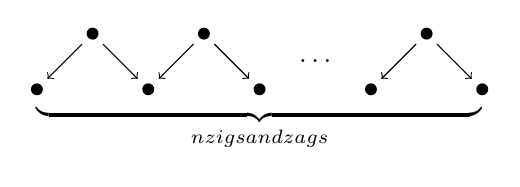
\begin{tikzpicture}[x=0.707cm,y=0.707cm,line cap=round]
			\fill (0,0) circle (0.5ex) coordinate (00);
			\fill (2,0) circle (0.5ex) coordinate (01);
			\fill (4,0) circle (0.5ex) coordinate (02);
			\fill (6,0) circle (0.5ex) coordinate (03);
			\fill (8,0) circle (0.5ex) coordinate (04);
			\fill (1,1) circle (0.5ex) coordinate (10);
			\fill (3,1) circle (0.5ex) coordinate (11);
			\fill (7,1) circle (0.5ex) coordinate (13);
			\draw[to-,shorten <=1.25ex,shorten >=1.25ex] (00) -- (10);
			\draw[to-,shorten <=1.25ex,shorten >=1.25ex] (01) -- (10);
			\draw[to-,shorten <=1.25ex,shorten >=1.25ex] (01) -- (11);
			\draw[to-,shorten <=1.25ex,shorten >=1.25ex] (02) -- (11);
			\draw[to-,shorten <=1.25ex,shorten >=1.25ex] (04) -- (13);
			\draw[to-,shorten <=1.25ex,shorten >=1.25ex] (03) -- (13);
			\path (02) to  node[pos=0.5,shift={(0,0.5)}] {$\ldots$} (03);
			\path (00) to node[pos=0.5,below=0.5ex] {$\underbrace{\hspace{5.656cm}}_{n\text{ zigs and zags}}$} (04);
		\end{tikzpicture}
	\end{center}
	In general, if $\iota\colon [k]\monomorphism{} [\ell]$ is the inclusion of an interval, then it induces a fully faithful functor $\iota\colon J_k\morphism J_\ell$. Since the $J_i$ are finite and $\Cc$ has finite limits and colimits, $\iota^*\colon \Fun(J_\ell,\Cc)\morphism \Fun(J_k,\Cc)$ has both adjoints, given by left and right Kan extension, and they are fully faithful again by \cref{cor:FullyFaithfulKanExtension}, Thus $Q_\ell(\Cc)\morphism Q_k(\Cc)$ is a split Verdier projection by \cref{thm:VerdierStuff}\itememph{b}. This clearly applies in our case, whence we're done.
\end{proof}
\begin{thm}[Waldhausen's additivity theorem]\label{thm:Additivity}
	If $F\colon \Cat_\infty^\mathrm{st}\morphism\An$ is additive, then so is
	\begin{equation*}
		\big|\Span^F(-)\big|\colon \Cat_\infty^\mathrm{st}\morphism \An\,.
	\end{equation*}
	In particular, $k\colon \Cat_\infty^\mathrm{st}\morphism \An$ is additive.
\end{thm}
This particular general formulation of the additivity theorem, or to be really precise, its further generalisation to Poincaré categories, first appeared in \cite[Theorem~2.4.1]{9author2}. But of course the original formulation (with $F\simeq \core$) is due to Waldhausen.
\begin{proof}[Proof of \cref{thm:Additivity}]
	The \enquote{in particular} follows as $k(\Cc)\simeq \Omega\left|\Span(\Cc)\right|\simeq \Omega\left|\Span^{\core}(\Cc)\right|$ by \cref{prop:QvsS}, $\core$ is additive by \cref{par:MoreOnTwAr}\itememph{d}, and $\Omega$ preserves pullbacks. The proof of the main statement consists of four steps.
	\begin{alphanumerate}
		\item[\itememph{1}] \itshape We prove that if $p\colon \Cc\morphism\Dd$ is a split Verdier projection, then it is  a bicartesian fibration \embrace{i.e.\ both cartesian and cocartesian}.
	\end{alphanumerate}

	This step is basically a consequence of the following simple lemma.
	\begin{lem}\label{lem:CocartesianLemma}
		Let $g\colon \Bb\shortdoublelrmorphism\Aa\noloc f$ be an adjoint pair in $\Cat_\infty$, with counit $c\colon gf\Rightarrow\id_\Aa$.
		\begin{alphanumerate}
			\item A morphism $\phi\colon x\morphism y$ in $\Aa$ is $f$-cocartesian iff the square
			\begin{equation*}
				\begin{tikzcd}
					gf(x)\rar["gf(\phi)"]\dar["c"']\drar[pushout] & gf(y)\dar["c"]\\
					x\rar["\phi"] & y
				\end{tikzcd}
			\end{equation*}
			is a pushout in $\Aa$.
			\item If $\Aa$ admits pushouts, $f$ preserves pushouts, and $g$ is fully faithful, then $f$ is a cocartesian fibration.
		\end{alphanumerate}
	\end{lem}
	\begin{proof}[Proof of \cref{lem:CocartesianLemma}]
		For \itememph{a}, plug the $(g,f)$-adjunction into the pullback square from \cref{def:WeirdCocartesianDefinition}\itememph{a}. For \itememph{b}, let $\phi'\colon x'\morphism y'$ be a morphism in $\Bb$ and let $x\in \Aa$ with $f(x)\simeq x'$ be given. Since $g$ is fully faithful, we have $y'\simeq fg(y')$, hence the morphism $\phi'\colon f(x)\morphism y'$ induces a morphism $gf(x)\morphism g(y')$ by adjunction. Now form the pushout
		\begin{equation*}
			\begin{tikzcd}
				gf(x)\rar \dar["c"']\drar[pushout] & g(y')\dar\\
				x\rar["\phi"] & y
			\end{tikzcd}
		\end{equation*}
		in $\Aa$. Note that $f(c)\colon fgf(x)\morphism f(x)\simeq x'$ is equivalent to the identity on $x'$ since $g$ is fully faithful. Moreover, $f$ preserve pushouts. Therefore, applying $f$ to the pushout square above gives a pushout
		\begin{equation*}
			\begin{tikzcd}
				x'\eqar[d] \rar["\phi'"]\drar[pushout] & y'\dar\\
				x\rar["f(\phi)"] & y
			\end{tikzcd}
		\end{equation*}
		Hence $f(\phi)\simeq \phi'$, so $\phi\colon x\morphism y$ is a lift of $\phi'$. By \itememph{a}, it is even an $f$-cocartesian lift, proving that $f$ is indeed a cocartesian fibration.
	\end{proof}
	Now we resume the proof of \cref{thm:Additivity}. Applying \cref{lem:CocartesianLemma}\itememph{b} to $p$ and its fully faithful left adjoint (which are exact functors between stable $\infty$-categories, so all assumptions are verified) shows that $p$ is a cocartesian fibration. By a dual argument applied to $p$ and its fully faithful right adjoint, $p$ is also cartesian. This finishes Step~\itememph{1}.
	\begin{alphanumerate}
		\item[\itememph{2}] \itshape We prove that if $p\colon \Cc\morphism\Dd$ is a split Verdier projection \embrace{thus an exact bicartesian fibration by Step~\itememph{1}}, then 
		\begin{equation*}
			\Span^F(p)\colon \Span^F(\Cc)\morphism\Span^F(\Dd)
		\end{equation*}
		is a  bicartesian fibration as well.
	\end{alphanumerate}

	\lecture[End of the proof of the additivity theorem. Group completion for additive functors. Rezk's equifibrancy lemma.]{2021-02-09}Let's first discuss the case $F\simeq \core$, which is of course the one of most interest to us, since it leads to $K$-theory, but it will also be half of the argument for the general case. We claim:
	\begin{alphanumerate}
		\item[\itememph{\boxtimes}]\itshape A morphism $x\morphism z$ in $\Span(\Cc)$, i.e., a span $x\lmorphism y\morphism z$ in $\Cc$, is $\Span(p)$-cocartesian if $y\morphism x$ is $p$-cartesian and $y\morphism z$ is $p$-cocartesian.
	\end{alphanumerate}
	Unravelling what a map $\Lambda_0^2\morphism \Span(\Cc)$ and a map $\Delta^2\morphism\Span(\Dd)$ look like, we have to show the following: Suppose we're given two solid diagrams
	\begin{equation*}
		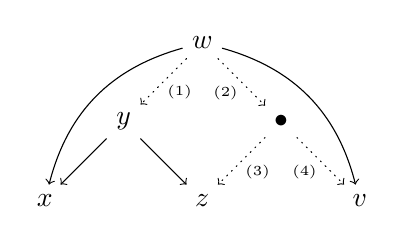
\begin{tikzpicture}[x=1cm,y=1cm,line cap=round,baseline=(10.base)]
			\node (00) at (0,0) {$x$};
			\node (01) at (2,0) {$z$};
			\node (02) at (4,0) {$v$};
			\node (10) at (1,1) {$y$};
			\node (11) at (3,1) {$\bullet$};
			\node (20) at (2,2) {$w$};
			\draw[-to] (10) to (00);
			\draw[-to] (10) to (01);
			\draw[-to,dotted] (20) to node[pos=0.5,below right=-0.5ex] {$\scriptscriptstyle (1)$} (10);
			\draw[-to,dotted] (20) to node[pos=0.5,below left=-0.5ex] {$\scriptscriptstyle (2)$} (11);
			\draw[-to,dotted] (11) to node[pos=0.5,below right=-0.5ex] {$\scriptscriptstyle (3)$} (01);
			\draw[-to,dotted] (11) to node[pos=0.5,below left=-0.5ex] {$\scriptscriptstyle (4)$} (02);
			\node[dotted,rotate=-45] at (2,1) {$\scriptstyle\pullbacksign$};
			\draw[-to,bend right] (20) to (00);
			\draw[-to,bend left] (20) to (02);
		\end{tikzpicture}\quad\overset{p}{\longmapsto}\quad
		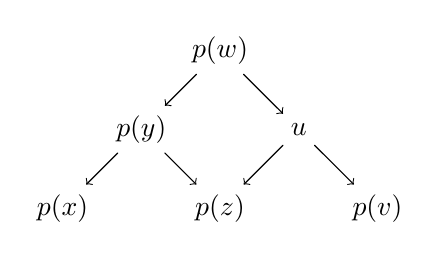
\begin{tikzpicture}[x=1cm,y=1cm,line cap=round,baseline=(10.base)]
			\node (00) at (0,0) {$p(x)$};
			\node (01) at (2,0) {$p(z)$};
			\node (02) at (4,0) {$p(v)$};
			\node (10) at (1,1) {$p(y)$};
			\node (11) at (3,1) {$u$};
			\node (20) at (2,2) {$p(w)$};
			\draw[-to] (10) to (00);
			\draw[-to] (10) to (01);
			\draw[-to] (20) to (10);
			\draw[-to] (20) to (11);
			\draw[-to] (11) to (01);
			\draw[-to] (11) to (02);
			\node[rotate=-45] at (2,1) {$\scriptstyle\pullbacksign$};
		\end{tikzpicture}
	\end{equation*}
	in $\Cc$ and $\Dd$, respectively, such that the left one is mapped into the right one under $p$. We must show that we can fill in all the dotted arrows (along with the missing object $\bullet$) in the left diagram in such a way that the square in the middle becomes a pullback. We can fill in the dotted arrow labelled \enquote{$(1)$} since $y\morphism x$ is $p$-cartesian. Next, we can choose the dotted arrow \enquote{$(2)$} to be a $p$-cocartesian lift of $p(w)\morphism u$. Since $w\morphism \bullet$ is now $p$-cocartesian, we can fill in the two missing dotted arrows \enquote{$(3)$} and \enquote{$(4)$}. Playing around with \cref{def:WeirdCocartesianDefinition}\itememph{a} easily shows that the square in the middle is a pushout iff $w\morphism \bullet$ is $p$-cocartesian. Hence it is a pushout by construction, and thus also a pullback since $\Cc$ is a stable $\infty$-category. This proves \itememph{\boxtimes}. Let us also remark that our argument shows that filling in the dotted arrows is unique up to contractible choice. Indeed, this is clear for \enquote{$(1)$}, \enquote{$(3)$}, and \enquote{$(4)$}, and for \enquote{$(2)$} we've just argued that we need to choose $w\morphism \bullet$ as a $p$-cocartesian lift of $p(w)\morphism u$ to make the middle square a pullback.
	
	We can now conclude that $\Span(p)\colon \Span(\Cc)\morphism \Span(\Dd)$ is a bicartesian fibration. Indeed, $p$ is bicartesian by Step~\itememph{1}, and given any span $p(x)\lmorphism y'\morphism z'$ in $\Dd$, we can lift the left map to a $p$-cartesian edge $y\morphism x$, and then the right map to a $p$-cocartesian edge $y\morphism z$, which proves that $\Span(p)$ is a cocartesian fibration by \itememph{\boxtimes}. Dualising the argument shows that $\Span(p)$ is also cartesian.
	
	
	Now for the general case. Let $\Ee\subseteq Q_1(\Cc)\simeq \Fun(J_1,\Cc)$ be the full sub-$\infty$-category where the left edge is $p$-cartesian and the right edge is $p$-cocartesian. Then the diagram
	\begin{equation*}
		\begin{tikzcd}
			\Ee\dar["p"']\rar["d_1"]\drar[pullback] & \Cc\dar["p"]\\
			Q_1(\Dd)\rar["d_1"] & \Dd
		\end{tikzcd}
	\end{equation*}
	is a pullback. Informally, this is because we can lift any span $(p(x)\lmorphism y'\morphism z')\in Q_1(\Dd)$ to a span $(x\lmorphism y\morphism z)\in \Ee$ as argued in the previous paragraph, and this lift is necessarily unique up to contractible choice since so is taking $p$-cartesian and $p$-cocartesian lifts. For a more formal argument, you would have to show that the map from $\Ee$ to the pullback is fully faithful and essentially surjective. Essential surjectivity follows from the argument we've just given. For fully faithfulness, use \cref{cor:HomInFunctorCats} to compute $\Hom$ anima in $Q_1(\Cc)$ and $Q_1(\Dd)$ (we have $\TwAr(J_1)\simeq J_2^\op$, so the formula really is not too bad) and then simplify using the pullback square from \cref{def:WeirdCocartesianDefinition}\itememph{a} and its dual for cartesian edges. I'll leave working out the details to you.
	
	Likewise, we get a pullback diagram
	\begin{equation*}
		\begin{tikzcd}
			\Ee\times_{Q_1(\Cc)}Q_2(\Cc)\dar["p"']\rar["{(\id_\Ee,d_1)}"]\drar[pullback] & \Ee\times_\Cc Q_1(\Cc)\dar["p"]\\
			Q_2(\Dd)\rar["{(d_2,d_1)}"] & Q_1(\Dd)\times_\Dd Q_1(\Dd)
		\end{tikzcd}
	\end{equation*}
	where the fibre product in the upper left corner is formed using $d_2\colon Q_2(\Cc)\morphism Q_1(\Cc)$. Informally, this square being a pullback is precisely what we proved in \itememph{\boxtimes}. Indeed, $\Ee\times_\Cc Q_1(\Cc)$ encodes the data of the diagram without the dotted arrows filled in, $Q_2(\Dd)$ encodes the data of the solid diagram in $\Dd$, and $Q_1(\Dd)\times_\Dd Q_1(\Dd)$ makes sure these two are compatible under $p$. We've seen in \itememph{\boxtimes} that it's always possible to fill in the dotted arrows, so that we obtain an object of $\Ee\times_{Q_1(\Cc)}Q_2(\Cc)$. Moreover, this object is unique up to contractible choice, as we've noted at the end of the proof of \itememph{\boxtimes}. This is the informal reason why $\Ee\times_{Q_1(\Cc)}Q_2(\Cc)$ is the pullback. To make this argument formal, you would again have to show that the map from $\Ee\times_{Q_1(\Cc)}Q_2(\Cc)$ to the pullback is fully faithful and essentially surjective. Essential surjectivity follows from the informal argument, and for fully faithfulness you have to compute $\Hom$ anima again using \cref{cor:HomInFunctorCats} (and even $\Hom$ anima in $Q_2(\Cc)$ are not too bad since limits over $\TwAr(J_2)\simeq J_3^\op$ are very manageable).
	
	Long story short, we get two pullback squares. But in fact they are split Verdier squares! Indeed, by \labelcref{par:EvenMoreOnVerdierSequences}, we only need to check that $\Cc\morphism \Dd$ and $\Ee\times_\Cc Q_1(\Cc)\morphism Q_1(\Dd)\times_\Dd Q_1(\Dd)$ are split Verdier projection. For the first one, this holds by assumption. The second one is a pullback of $Q_1(\Cc)\morphism Q_1(\Dd)$ (using the first pullback square), which is a split Verdier projection because the fully faithful left and right adjoints of $\Cc\morphism \Dd$ extend to functor $\infty$-categories.
	
	Thus, both diagrams stay pullback squares after applying the additive functor $F$. The second diagram then witnesses that the image of
	\begin{equation*}
		F(\Ee)\morphism F\big(Q_1(\Cc)\big)\morphism \Hom_{\Cat_\infty}\big([1],\Span^F(\Cc)\big)
	\end{equation*}
	consists of $\Span^F(p)$-cocartesian edges (essentially by running the above arguments backwards), and the first diagram gives a sufficient supply of these. This shows that $\Span^F(p)$ is indeed a cocartesian fibration. By a dual argument we see that it is cartesian as well. This finishes Step~\itememph{2}.
	
	
	
	
	
	\begin{alphanumerate}
		\item[\itememph{3}] \itshape We prove that the functor $|\blank|\colon \Cat_\infty\morphism\An$ preserves pullback squares if one of the legs is a bicartesian fibration.
	\end{alphanumerate}

	This step is easy again. Suppose we're given a pullback
	\begin{equation*}
		\begin{tikzcd}
			\Aa\dar\rar\drar[pullback] &\Bb\dar\\
			\Cc\rar["p"] & \Dd
		\end{tikzcd}
	\end{equation*}
	in $\Cat_\infty$, such that  $\Bb\morphism \Dd$ and thus also $\Aa\morphism \Cc$ are bicartesian fibrations. We denote by $F\coloneqq \St^\cocart(\Bb\morphism\Dd)\colon \Dd\morphism \Cat_\infty$ be the cocartesian straightening of $\Bb\morphism\Dd$. Since unstraightening turns compositions into pullbacks, we obtain
	\begin{equation*}
	%	\begin{tikzcd}
	%		\Un^\cocart(F\circ p)\dar\rar\drar[pullback] &\Un^\cocart(F)\dar\\
	%		\Cc\rar["p"] & \Dd
	%	\end{tikzcd}
		\Un^\cocart(F\circ p)\simeq \Aa\quad\text{and}\quad \Un^\cocart(F)\simeq \Bb\,.
	\end{equation*}
	Now consider the diagram
	\begin{equation*}
		\begin{tikzcd}
			\Dd\rar["F"]\dar &\Cat_\infty\rar["{|\blank|}"] & \An\\
			{|\Dd|}\ar[urr,bend right=15,dashed,"{|F|}"']
		\end{tikzcd}
	\end{equation*}
	Note that since $F$ is a bicartesian fibration, every morphism $\phi\colon x\morphism y$ in $\Dd$ is sent to a left-adjoint functor $F(\phi)\colon F(x)\morphism F(y)$, hence to an equivalence $|F(\phi)|\colon |F(x)|\isomorphism |F(y)|$. Hence the dashed arrow exists by the universal property of localisations of $\infty$-categories.
	
	By unstraightening of functors into $\An$, we now get a pullback diagram
	\begin{equation*}
		\begin{tikzcd}
			\Un^\mathrm{left}\big(|F|\circ |p|\big)\dar\rar\drar[pullback] &\Un^\mathrm{left}\big(|F|\big)\dar\\
			{|\Cc|}\rar["{|p|}"] & {|\Dd|}
		\end{tikzcd}
	\end{equation*}
	So we're done if we can show that $\Un^\mathrm{left}(|F|)$ and $\Un^\mathrm{left}(|F|\circ |p|)$ are the realisations of $\Un^\cocart(F)$ and $\Un^\cocart(F\circ p)$, respectively. The easiest way to see this is probably \cref{prop:CoLimitsInCat}: We know that $\colimit(F\colon \Dd\morphism \Cat_\infty)$ is some localisation of $\Un^\cocart(F)$, hence
	\begin{align*}
		\left|\Un^\cocart(F)\right|\simeq \Big|\colimit\Big(\Dd\morphism[F] \Cat_\infty\Big)\Big|&\simeq \colimit\Big(\Dd\morphism[F] \Cat_\infty\morphism[|\blank|]\An\Big)\\
		&\simeq \colimit\Big(|\Dd|\morphism[|F|] \An\Big)\\
		&\simeq \Un^\mathrm{left}\big(|F|\big)\,,
	\end{align*}
	as desired. The second equivalence follows from the fact that $|\blank|\colon \Cat_\infty\morphism \An$, being a left adjoint, preserves colimits. For the third equivalence, we use that the localisation $\Dd\morphism|\Dd|$ is cofinal, as we noted after \cref{def:cofinal}. For $\Un^\cocart(F\circ p)$ we can use a similar argument. This finishes Step~\itememph{3}.
	\begin{alphanumerate}
		\item[\itememph{4}] \itshape We prove that $\Span^F(-)$ sends split Verdier squares to pullbacks in $\Cat_\infty$ and finish the proof of \cref{thm:Additivity}.
	\end{alphanumerate}

	If we can show the first assertion, then a combination of Step~\itememph{2} and~\itememph{3} seals the deal. Recall that $\Span^F\simeq \asscat(F(Q(-)))$ by \cref{lem:SpanF}. So let
	\begin{equation*}
		\begin{tikzcd}
			\Aa\dar\rar\drar[pullback] &\Bb\dar\\
			\Cc\rar & \Dd
		\end{tikzcd}
	\end{equation*}
	be a split Verdier square. We know that $Q_n(-)\colon \Catst\morphism\Catst$ preserves split Verdier squares for all $n\in\IN$ (because $Q_n(-)\simeq \Fun(J_n,-)$ preserves pullbacks and the required fully faithful adjoints extend to functor $\infty$-categories) and $F$ turns them into pullbacks in $\An$, hence
	\begin{equation*}
		\begin{tikzcd}
			F \big(Q(\Aa)\big)\dar\rar\drar[pullback] &F\big(Q(\Bb)\big)\dar\\
			F\big(Q(\Cc)\big)\rar & F\big(Q(\Dd)\big)
		\end{tikzcd}
	\end{equation*}
	is a pullback in $\cat{sAn}$. In fact, it is even a Segal anima by \cref{lem:SpanF}. However, $\asscat(-)\colon \cat{sAn}\morphism \Cat_\infty$ doesn't necessarily preserve pullbacks of incomplete Segal anima. However, the canonical (up to contractible choice) morphism
	\begin{equation*}
		\asscat(X\times_YZ)\morphism \asscat(X)\times_{\asscat(Y)}\asscat(Z)
	\end{equation*}
	is always fully faithful for Segal anima $X,Y,Z\in\cat{sAn}$, as follows from \cref{eq:asscat2}. So only essential surjectivity can go wrong. Recall that $\core \asscat(X)\simeq |X^\times|$ for $X$ Segal by \cref{eq:asscat1}. We claim that
	\begin{equation*}
		\pi_0\left|X^\times\times_{Y^\times}Z^\times\right|\morphism \pi_0\left(|X^\times|\times_{|Y^\times|}|Z^\times|\right)
	\end{equation*}
	is surjective if $\asscat(X)\morphism\asscat(Y)$ is a bicartesian fibration, which will be sufficient for our case by Step~\itememph{2}. Every connected component on the right-hand side can be represented by points $x\in X_0$, $z\in Z_0$, and a path in $|Y^\times|$ connecting their images. To see why the $0$-skeleta already hit all path components, take a look again at the skeletal method in the proof of \cref{lem:SkeletalInduction}, and in particular, at \cref{eq:SkeletalInduction}. Again by considering skeleta, we see that two points belonging to the same path component in $|Y^\times|$ is already determined by $Y_1^\times$. Hence there are edges $y_i\in Y_1^\times$ and a path $w$ in $Y_0$ that connect $x$ and $z$ via
	\begin{equation*}
		x\morphism[y_1]s_1\lmorphism[y_2]s_2\morphism[y_3]\dotso \xleftarrow{y_{2n}}s_{2n}\overset{w}{\longrightsquigarrow{\morphismlength-0.145em}} z
	\end{equation*}
	Using that $\asscat(X)\morphism\asscat(Y)$ is a bicartesian fibration, we can lift this to a similar sequence in $X$, which gives a connected component in $\pi_0|X^\times\times_{Y^\times}Z^\times|$. This shows the desired surjectivity and the proof is finally done!
\end{proof}

We're now almost in position to prove \cref{thm:K=coreGrp}. But Fabian decided to give a brief discussion of grouplike additive functors and their span $\infty$-categories first. To make the result of that discussion more comprehensible, I put them into a separate lemma.
\begin{lem}\label{lem:GrouplikeFunctors}
	Suppose $F\colon \Catst\morphism \An$ is a grouplike additive functor and let $\Cc$ be a stable $\infty$-category. Then
	\begin{equation*}
		F\big(\Ar(\Cc)\big)\simeq F(\Cc)\times F(\Cc)\quad\text{and}\quad F\big(Q_n(\Cc)\big)\simeq F(\Cc)^{2n+1}
	\end{equation*}
	for all $n\in\IN$. More generally, there's an equivalence
	\begin{equation*}
		\operatorname{Bar}\big(*,F(\Cc)\times F(\Cc),F(\Cc)\big)\isomorphism F\big( Q(\Cc)\big)\,.
	\end{equation*}
	Finally, $\Span^F(\Cc)\simeq B F(\Cc)$ \embrace{so in particular $\Span^F(\Cc)$ is a connected anima}.
\end{lem}
\begin{proof}[Proof sketch]
	The equivalence $F(\Ar(\Cc))\simeq F(\Cc)\times F(\Cc)$ follows from the stable recollement from \cref{par:Recollements} together with \cref{par:MoreOnVerdierSequences}\itememph{d^*}. The equivalence $F(Q_n(\Cc))\isomorphism F(\Cc)^{2n+1}$ is induced by evaluation $Q_n(\Cc)\simeq \Fun(J_n,\Cc)\morphism \Cc$ at the $2n+1$ objects of $J_n$. To see that it is indeed an equivalence, let's first consider the case $n=1$. In this case we have a split Verdier sequence $\Cc\morphism Q_1(\Cc)\morphism \Ar(\Cc)$ (adjoints are given by left/right Kan extension along $[1]\morphism J_1$), which proves $F(Q_1(\Cc))\simeq F(\Cc)^3$ by \cref{par:MoreOnVerdierSequences}\itememph{d^*}. The general case follows either by induction, or by the an iterative application of the split Verdier square from \cref{lem:SpanF}.
	
	We've seen in \cref{par:MoreOnVerdierSequences}\itememph{c} that $F(\Cc)$ has a canonical $\IE_\infty$-group structure. Moreover, its addition map $\oplus\colon F(\Cc)\times F(\Cc)\morphism F(\Cc)$ turns $F(\Cc)$ into a left module over $F(\Cc)\times F(\Cc)$.  We may thus form $\operatorname{Bar}(*,F(\Cc)\times F(\Cc),F(\Cc))\colon \IDelta^\op\morphism \CGrp(\An)$ as in \labelcref{par:BarConstruction}. By construction, it satisfies
	\begin{equation*}
		\operatorname{Bar}_n\big(*,F(\Cc)\times F(\Cc),F(\Cc)\big)\simeq F(\Cc)^{2n+1}\,,
	\end{equation*}
	so it coincides degreewise with $F( Q(\Cc))$. But $\operatorname{Bar}(*,F(\Cc)\times F(\Cc),F(\Cc))$ is also left-Kan extended from its restriction along $\IDelta_{\mathrm{inj},\leq 1}^\op\morphism \IDelta^\op$, so it's easy to construct a functor from it into $F( Q(\Cc))$, which is then a degreewise equivalence.
	
	From the description as a bar complex, or just by checking directly, one can verify that
	\begin{equation*}
		F\big(Q_1(\Cc)\big)^\times\simeq F\big(Q_1(\Cc)\big)\,.
	\end{equation*}
	 Hence $\Span^F(\Cc)\simeq \asscat\big(F (Q(\Cc))\big)$is an anima (combine \cref{thmdef:RezkNerve}\itememph{c} with \cref{eq:asscat2} to see that all edges are equivalences). Moreover, it is connected. In fact, it's true that $|\Span^F(\Cc)|$ is connected for every additive functor $F$. To see this, use \cref{rem:Realisation}, \cref{prop:QvsS}, and \labelcref{par:edgewiseSubdivision} (in that order) to obtain
	\begin{equation*}
		\big|\Span^F(\Cc)\big|\simeq \left|F\big(Q(\Cc)\big)\right|\simeq \big|F\big(S(\Cc)\big)^\mathrm{esd}\big|\simeq \left|F\big(S(\Cc)\big)\right|\,.
	\end{equation*}
	Now $\pi_0F(S_0(\Cc))\morphism \pi_0\left|F(S(\Cc))\right|$ is surjective, see claim~\itememph{*} in the proof of \cref{prop:CompletionOfMonoidsFullyFaithful}. But $S_0(\Cc)\simeq *$, hence indeed $\pi_0\left|F(S(\Cc))\right|=0$.
	
	%To see this, we first note $\Span^F(\Cc)\simeq \core (\asscat(F (Q(\Cc))))\simeq |F(Q(\Cc))^\times|$ by \cref{eq:asscat1}. Now $\pi_0$ of the right-hand side can be computed as described in , the result being
	%\begin{align*}
	%	\pi_0\big|F\big(Q(\Cc)\big)^\times\big|&= \Coeq\left(\pi_0F\big(Q_1(\Cc)\big)^\times\doublemorphism[d_1][d_0] \pi_0F\big(Q_0(\Cc)\big)^\times\right)\\
	%	&=\Coeq\left(\pi_0F\big(Q_1(\Cc)\big)\doublemorphism[d_1][d_0] \pi_0F\big(Q_0(\Cc)\big)\right)\\
	%	&=\Coeq\left(\pi_0F(\Cc)^3\doublemorphism[\pr_1][\pr_3] \pi_0F(\Cc)\right)\,,
	%\end{align*}
	%which evidently vanishes.
	Back in the situation where $F$ is grouplike, we see that to prove $\Span^F(\Cc)\simeq BF(\Cc)$, it suffices to compute that $\Omega_0\Span^F(\Cc)\simeq F(\Cc)$ by \cref{par:Grp(An)=(*/An)Connected}. Now $\Omega_0\Span^F(\Cc)$ coincides with $\Hom_{\Span^F(\Cc)}(0,0)$. To compute this, consider\begin{equation*}
		\begin{tikzcd}
			\Cc\dar\rar\drar[pullback] & Q_1(\Cc)\dar["{(d_1,d_0)}"]\\
			0\rar & Q_0(\Cc)\times Q_0(\Cc)
		\end{tikzcd}
	\end{equation*}
	It is a pullback by inspection, as there are $\Cc$ possibilities to fill in the missing spot in a span $0\lmorphism \bullet\morphism 0$.
	It is even a split Verdier square, since the right vertical arrow has both adjoints, given by left and right Kan extension, which are both fully faithful (in fact, both adjoints agree and send a pair $(x,y)\in Q_0(\Cc)\times Q_0(\Cc)\simeq \Cc\times \Cc$ to the span $x\lmorphism x\oplus y\morphism y$ in $Q_1(\Cc)\simeq \Fun(J_1,\Cc)$). So the pullback property is preserved upon applying $F$. But after applying $F$, the new pullback diagram computes $\Hom_{\Span^F(\Cc)}(0,0)$ by \cref{eq:asscat2}.
\end{proof}
Fabian remarks that the special case $k(\Ar(\Cc))\simeq k(\Cc)\times k(\Cc)$ of \cref{lem:GrouplikeFunctors} is the content of Waldhausen's original additivity theorem. Moreover, we've seen in the proof that $F(Q_1(\Cc))^\times\simeq F(Q_1(\Cc))$ for every grouplike additive functor $F$. This tells us that the Segal anima $F (Q(\Cc))$ is seldom complete: By \cref{thmdef:RezkNerve}\itememph{c}, we would need that
\begin{equation*}
	F(\Cc)\simeq F\big(Q_0(\Cc)\big)\isomorphism F\big(Q_1(\Cc)\big)^\times\simeq F(\Cc)^3
\end{equation*}
is an equivalence, which only holds if $F(\Cc)\simeq 0$.
\begin{thm}\label{thm:SpanF}
	If $F\colon \Catst\morphism\An$ is grouplike and additive and $\Cc$ is a stable $\infty$-category $\Cc$, then applying the realisation functor $|\blank|\colon \Cat_\infty\morphism \An$ to the pullback square
	\begin{equation*}
		\begin{tikzcd}
			\Hom_{\Span^F(\Cc)}(0,0)\rar\dar\drar[pullback] & 0/\Span^F(\Cc)\dar\\
			*\rar["0"] & \Span^F(\Cc)
		\end{tikzcd}
	\end{equation*}
	in $\Cat_\infty$ gives a pullback square
	\begin{equation*}
		\begin{tikzcd}
			F(\Cc)\rar\dar\drar[pullback] & *\dar["0"]\\
			*\rar["0"] & {|\Span^F(\Cc)|}
		\end{tikzcd}
	\end{equation*}
	in $\An$. So in particular, $F(\Cc)\simeq \Omega |\Span^F(\Cc)|$.
\end{thm}
\begin{proof}[First proof]
	We've checked (or at least sketched) in \cref{lem:GrouplikeFunctors} that
	\begin{equation*}
		\Span^F(\Cc)\simeq |\Span^F(\Cc)|\simeq BF(\Cc)\,.
	\end{equation*}
	But $F(\Cc)$ is already an $\IE_\infty$-group by assumption, so $\Omega BF(\Cc)\simeq F(\Cc)$ follows from \cref{cor:CommutativeHorizontalAdjoints}\itememph{c}. A posteriori, this implies that the square in question is indeed a pullback.
\end{proof}
With that, we can finally prove the theorem of Blumberg--Gepner--Tabuada.
\begin{proof}[Proof of \cref{thm:K=coreGrp}]\label{page:ProofOfBlumbergGepnerTabuada}
	First note that $\Omega|\Span^F(-)|$ is additive again for any additive functor $F$, since it is the composition of the additive functor $|\Span^F(-)|$ (\cref{thm:Additivity}) with the limits-preserving functor $\Omega\colon \CMon(\An)\morphism \CGrp(\An)$ (\cref{cor:CommutativeHorizontalAdjoints}\itememph{b}). This also shows that $\Omega|\Span^F(-)|$ takes values in the grouplikes.
	
	As always, we'll use Proposition~\labelcref{prop:LLaddendum} to prove that 
	\begin{equation*}
		L\simeq \Omega |\Span^{(-)}(-)|\colon \Fun^\add(\Catst,\An)\morphism \Fun^\grp(\Catst,\An)
	\end{equation*}
	is a left Bousfield localisation. First, we need a natural transformation $\eta\colon \id \Rightarrow L$. The computation in the proof of \cref{lem:GrouplikeFunctors} shows $F(\Cc)\simeq \Hom_{\Span^F(\Cc)}(0,0)$ for all additive functors $F$ (although we assumed that $F$ is grouplike there, but this isn't needed in the computation). Composing with the natural map 
	\begin{equation*}
		\Hom_{\Span^F(\Cc)}(0,0)\morphism \Hom_{|\Span^F(\Cc)|}(0,0)\simeq \Omega|\Span^F(\Cc)|
	\end{equation*}
	gives a map $F(\Cc)\morphism \Omega|\Span^F(\Cc)|$ which is functorial in $\Cc$ and $F$, thus providing the required transformation $\eta\colon \id\Rightarrow L$. Now \cref{thm:SpanF} implies that $\eta L,L\eta\colon L\overset{\sim}{\Longrightarrow} L\circ L$ are both equivalences, whence $L$ is indeed a left Bousfield localisation. Its essential image is contained in the grouplike functors as checked above, hence equals the grouplike functors since \cref{thm:SpanF} precisely says that $\eta$ is an equivalence on grouplikes.
\end{proof}
As the \enquote{first proof} above suggests, we will give a second proof of \cref{thm:SpanF}. The second proof won't rely on the sketchy parts of \cref{lem:GrouplikeFunctors} (at the price of being much longer), but more importantly, it will introduce some tools that we'll need later. Where the first proof showed $F\simeq \Omega|\Span^F(-)|$ right away and then deduced the pullback property afterwards, the second proof will verify the pullback property directly. The key to still getting pullbacks after taking colimits is Rezk's equifibrancy lemma.
\begin{lemdef}[Rezk]\label{lemdef:Equifibred}
	Let $\Ii$ be any $\infty$-category \embrace{which we think of as a digram shape}. Suppose we're given a pullback square
	\begin{equation*}
		\begin{tikzcd}
			A\rar\dar["\sigma"']\drar[pullback] & B\dar["\tau"]\\
			C\rar & D
		\end{tikzcd}
	\end{equation*}
	in $\Fun(\Ii,\An)$ such that $\tau$ us \emph{equifibred}, i.e.\ such that
	\begin{equation*}
		\begin{tikzcd}
			B_i\rar\dar \drar[pullback] & B_j\dar \\
			D_i\rar & D_j
		\end{tikzcd}
	\end{equation*}
	is a pullback for all morphisms $i\morphism j$ in $\Ii$. Then also the diagram
	\begin{equation*}
		\begin{tikzcd}[row sep=scriptsize]
			\colimit\limits_{i\in\Ii} A\rar\dar[shorten <=-0.75ex,"\sigma"']\drar[pullback] & \colimit\limits_{i\in\Ii} B_i\dar[shorten <=-0.75ex,"\tau"]\\
			\colimit\limits_{i\in\Ii} C_i\rar & \colimit\limits_{i\in\Ii} D_i
		\end{tikzcd}
	\end{equation*}
	is a pullback in $\An$.
\end{lemdef}
\begin{proof}
	We first prove the following claim to get a description of $\colimit_\Ii B$.
	\begin{alphanumerate}
		\item[\itememph{\boxtimes}] \itshape Suppose $\tau$ is equifibred and let $K$ be any anima. Then a transformation $\eta\colon B\Rightarrow \const K$ together with a map $K\morphism \colimit_{i\in\Ii} D_i$ make the diagram
		\begin{equation*}
			\begin{tikzcd}
				B_i\rar\dar \drar[pullback] & K\dar \\
				D_i\rar & \colimit\limits_{i\in\Ii} D_i
			\end{tikzcd}
		\end{equation*}
		a pullback for each $i\in \Ii$ iff $\eta$ induces an equivalence $\colimit_{i\in\Ii} B_i\isomorphism K$.
	\end{alphanumerate}
	To prove \itememph{\boxtimes}, consider the functors $F_i\simeq \St^\mathrm{left}(B_i\morphism D_i)\colon D_i\morphism \An$. We claim that by equifibrancy of $\tau$, the $F_i$ assemble into a functor
	\begin{equation*}
		F\colon \colimit_{i\in\Ii} D_i\morphism \An\,.
	\end{equation*}
	On Sil's insistence, Fabian has given a proper argument for this in the official notes \cite[Chapter~IV p.\:46]{KTheory}, which I'll include here. The transformation $\tau$ corresponds to a map $[1]\morphism \Fun(\Ii,\An)$, which we may curry to a map $\Ii\morphism \Ar(\An)$. That $\tau$ is equifibrant means that this map sends all morphisms in $\Ii$ to morphisms in $\Ar(\An)$ which are represented by pullback squares in $\An$. On the other hand,
	\begin{equation*}
		\Fun\left(\colimit_{i\in\Ii}D_i,\An\right)\simeq \limit_{i\in \Ii^\op}\Fun(D_i,\An)\simeq \limit_{i\in\Ii^\op}\An/D_i
	\end{equation*}
	by straightening. Note that the functor $\An/-\colon \An^\op\morphism \Cat_\infty$ is not the usual slice category functor (whose codomain would be $\An$ rather than $\An^\op$). Indeed, to a map $i\morphism j$ in $\Ii$ we don't associate the forgetful functor $\An/D_i\morphism \An/D_j$, but the pullback functor $-\times_{D_j}D_i\colon\An/D_j\morphism \An/D_i$. Thus, $\An/-\colon\An^\op\morphism\Cat_\infty$ is represented by the cartesian (!) straightening of $t\colon \Ar(\An)\morphism \An$, which is in fact a cartesian fibration by \cref{exc:tCartesian}. Moreover, the $t$-cartesian edges are precisely the pullback squares, hence $\Ii\morphism \Ar(\An)$ sends every edge to a $t$-cartesian edge. Therefore, the induced map $\Ii\morphism \Ii\times_{\An}\Ar(\An)$ is a map of cartesian fibrations over $\Ii$, and thus it induces a natural transformation
	\begin{equation*}
		\left(\const *\Longrightarrow \An/D_{(-)}\right)\colon \Ii^\op\morphism \An\,.
	\end{equation*}
	This transformation induces a single map $*\morphism \limit_{i\in\Ii^\op}\An/D_i$, which provides the functor $F\colon \colimit_{i\in\Ii}\morphism \An$ we're looking for.
	
	Note that $\Un^\mathrm{left}(F)\morphism \colimit_{i\in \Ii}D_i$ is a left fibration over the anima $\colimit_{i\in \Ii}D_i$, hence $\Un^\mathrm{left}(F)$ is an anima itself. Thus $\Un^\mathrm{left}(F)\simeq |\Un^\mathrm{left}(F)|$, and we may apply  \cref{prop:CoLimitsInCat} twice to get
	\begin{align*}
		\Un^\mathrm{left}(F)\simeq \colimit_{\colimit_{i\in \Ii}D_i}F&\simeq \colimit_{i\in \Ii}\colimit_{D_i}D_i\\
		&\simeq \colimit_{i\in\Ii}\Un^\mathrm{left}(F_i)\\
		&\simeq \colimit_{i\in\Ii}B_i\,.
	\end{align*}
	This shows that $K\simeq\colimit_{i\in\Ii}B_i\simeq \Un^\mathrm{left}(F)$ does indeed fit into the pullback diagram from \itememph{\boxtimes}. Conversely, every $K\morphism \colimit_{i\in \Ii}D_i$ is uniquely determined by its pullbacks to the $D_i$, since  straightening implies $\An/\colimit_{i\in \Ii}D_i\simeq \Fun(\colimit_{i\in \Ii}D_i,\An)\simeq \limit_{i\in\Ii^\op}\An/D_i$, as seen above. So there is only one $K$ that fits into the pullbacks from \itememph{\boxtimes}, whence $K\simeq \colimit_{i\in \Ii}B_i$ is the only possibility. This shows \itememph{\boxtimes}.
	
	Now the actual proof may start. We first check that $\sigma$ is equifibred as well. To this end, let $i\morphism j$ be any morphism in $\Ii$ and consider the diagram
	\begin{equation*}
		\begin{tikzcd}[row sep=scriptsize]
			A_i\dar\rar\drar[dotted,pullback] & A_j\rar\dar\drar[pullback] &B_j\rar\dar\drar[pullback] & \colimit\limits_{i\in\Ii} B_i\dar[shorten <=-0.75ex,"\tau"]\\
			C_i\rar & C_j\rar & D_j\rar &\colimit\limits_{i\in\Ii} D_i
		\end{tikzcd}
	\end{equation*}
	We must show that the left square is a pullback. But the middle square is a pullback by assumption and the right one is a pullback by \itememph{\boxtimes}. Hence also the rectangle formed by the middle and the right square is a pullback. But then the same argument implies that also the rectangle formed by all three squares must be a pullback. By abstract pullback nonsense, this implies that the left square must be a pullback as well, as claimed. This shows that $\sigma$ is equifibred.
	
	Now consider the diagram
	\begin{equation*}
		\begin{tikzcd}[row sep=scriptsize]
			A_j\dar\rar\drar[dotted,pullback]   &\colimit\limits_{i\in\Ii}B_i\times_{\colimit_{i\in\Ii}D_i}\colimit\limits_{i\in\Ii}C_i\rar\dar[shorten <=-0.75ex]\drar[pullback] & \colimit\limits_{i\in\Ii} B_i\dar[shorten <=-0.75ex,"\tau"]\\
			C_j\rar & \colimit\limits_{i\in\Ii}C_i\rar &\colimit\limits_{i\in\Ii} D_i
		\end{tikzcd}
	\end{equation*}
	The right square is a pullback by construction, and that the outer rectangle is a pullback was checked in the previous step. Hence again the left square is a pullback too for all $j\in \Ii$. But then \itememph{\boxtimes} applied to $\sigma$ implies that $\colimit_{i\in\Ii}B_i\times_{\colimit_{i\in\Ii}D_i}\colimit_{i\in\Ii}C_i\simeq \colimit_{i\in\Ii}A_i$ and we're done!
\end{proof}
\begin{proof}[Second proof of \cref{thm:SpanF}]
	We split the proof into two major steps.
	\begin{alphanumerate}
		\item[\itememph{1}] \itshape We construct an easily understood Segal anima $\operatorname{Null}(\Cc)\colon \IDelta^\op\morphism\An$ satisfying
		\begin{equation*}
			\asscat\big(F(\operatorname{Null}(\Cc))\big)\simeq 0/\Span^F(\Cc)
		\end{equation*}
	\end{alphanumerate}
	
	Consider the functor $[0]\star -\colon \IDelta^\op\morphism \IDelta^\op$. It induces a functor $\operatorname{d\acute{e}c}\colon \cat{sAn}\morphism \cat{sAn}$, called the \emph{décalage}. It already appeared in the proof of \cref{prop:HStronglyMonoidal}, although our convention there was to consider $-\star[0]$ instead (but who cares). The décalage functor comes equipped with natural transformations
	\begin{equation*}
		p\colon \operatorname{d\acute{e}c}\Longrightarrow \const\ev_0\quad\text{and}\quad d_0\colon \operatorname{d\acute{e}c} \Longrightarrow \id\,,
	\end{equation*}
	induced by $[0]\subseteq [0]\star [n]$ and $[n]\subseteq [0]\star [n]$ for all $[n]\in \IDelta^\op$, respectively. One easily checks that for every Segal anima $X$ and all $x\in X_0$ one has a commutative diagram
	\begin{equation*}
		\begin{tikzcd}
			\asscat\big(\fib_x(p\colon \operatorname{d\acute{e}c} X\morphism \const X_0)\big)\dar["d_0"']\rar[iso] & x/\asscat(X) \dlar[bend left=15]\\
			\asscat(X) & 
		\end{tikzcd}
	\end{equation*}
	To see this, one first checks that $\fib_x(p\colon \operatorname{d\acute{e}c} X\morphism \const X_0)$ is Segal again, so the $\Hom$ anima in its associated category can be computed via \cref{eq:asscat2}. Once we understand the $\Hom$ anima in it, we find that $\asscat(\fib_x(p\colon \operatorname{d\acute{e}c} X\morphism \const X_0))$ has an initial element that's mapped to $x$ under $d_0$, hence $d_0$ lifts canonically to $x/\asscat(X)$. Then show that the lift is fully faithful and essentially surjective, again using that $\Hom$ anima can be calculated via \cref{eq:asscat2}. I leave the details to you since I'm too lazy to work them out.
	
	Now put 
	\begin{equation*}
		\operatorname{Null}(\Cc)\coloneqq \fib_0(p\colon \operatorname{d\acute{e}c}Q(\Cc)\rightarrow \const \Cc)\,.
	\end{equation*}
	So explicitly, $\operatorname{Null}_n(\Cc)\subseteq Q_{n+1}(\Cc)$ is the full sub-$\infty$-category spanned by diagrams of the following form (as usual, the dotted part is uniquely determined by the solid part):
	\begin{center}
		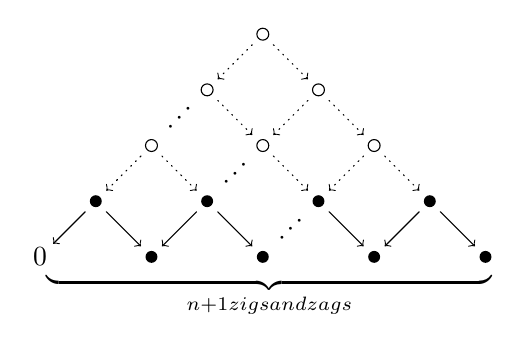
\begin{tikzpicture}[x=0.707cm,y=0.707cm,line cap=round]
			\node[inner sep=2] (00) at (0,0) {$0$};
			\fill (2,0) circle (0.5ex) coordinate (01);
			\fill (4,0) circle (0.5ex) coordinate (02);
			\fill (6,0) circle (0.5ex) coordinate (03);
			\fill (8,0) circle (0.5ex) coordinate (04);
			\fill (1,1) circle (0.5ex) coordinate (10);
			\fill (3,1) circle (0.5ex) coordinate (11);
			\fill (5,1) circle (0.5ex) coordinate (12);
			\fill (7,1) circle (0.5ex) coordinate (13);
			\draw[fill=white] (2,2) circle (0.5ex) coordinate (20);
			\draw[fill=white] (4,2) circle (0.5ex) coordinate (21);
			\draw[fill=white] (6,2) circle (0.5ex) coordinate (22);
			\draw[fill=white] (3,3) circle (0.5ex) coordinate (30);
			\draw[fill=white] (5,3) circle (0.5ex) coordinate (31);
			\draw[fill=white] (4,4) circle (0.5ex) coordinate (40);
			\draw[to-,shorten >=1.25ex] (00) -- (10);
			\draw[to-,shorten <=1.25ex,shorten >=1.25ex] (01) -- (10);
			\draw[to-,shorten <=1.25ex,shorten >=1.25ex] (01) -- (11);
			\draw[to-,shorten <=1.25ex,shorten >=1.25ex] (02) -- (11);
			\draw[to-,shorten <=1.25ex,shorten >=1.25ex,dotted] (10) -- (20);
			\draw[to-,shorten <=1.25ex,shorten >=1.25ex,dotted] (11) -- (20);
			\draw[to-,shorten <=1.25ex,shorten >=1.25ex] (03) -- (12);
			\draw[to-,shorten <=1.25ex,shorten >=1.25ex,dotted] (12) -- (21);
			\draw[to-,shorten <=1.25ex,shorten >=1.25ex,dotted] (21) -- (30);
			\draw[to-,shorten <=1.25ex,shorten >=1.25ex] (04) -- (13);
			\draw[to-,shorten <=1.25ex,shorten >=1.25ex,dotted] (13) -- (22);
			\draw[to-,shorten <=1.25ex,shorten >=1.25ex,dotted] (22) -- (31);
			\draw[to-,shorten <=1.25ex,shorten >=1.25ex,dotted] (31) -- (40);
			\draw[to-,shorten <=1.25ex,shorten >=1.25ex] (03) -- (13);
			\draw[to-,shorten <=1.25ex,shorten >=1.25ex,dotted] (12) -- (22);
			\draw[to-,shorten <=1.25ex,shorten >=1.25ex,dotted] (21) -- (31);
			\draw[to-,shorten <=1.25ex,shorten >=1.25ex,dotted] (30) -- (40);
			\path (02) to  node[pos=0.5,sloped] {$\ldots$} (12);
			\path (11) to  node[pos=0.5,sloped] {$\ldots$} (21);
			\path (20) to  node[pos=0.5,sloped] {$\ldots$} (30);
			\node[rotate=-45] at (2,1) {$\pullbacksign$};
			\node[rotate=-45] at (6,1) {$\pullbacksign$};
			\node[rotate=-45] at (5,2) {$\pullbacksign$};
			\node[rotate=-45] at (4,3) {$\pullbacksign$};
			\path (00) to node[pos=0.5,below=0.5ex] {$\underbrace{\hspace{5.656cm}}_{n+1\text{ zigs and zags}}$} (04);
		\end{tikzpicture}
	\end{center}
	Moreover, since $p\colon \operatorname{d\acute{e}c}Q(\Cc)\rightarrow \const \Cc)$ is a degreewise split Verdier projection (with left/right Kan extension as adjoints, as usual), we have 
	\begin{equation*}
		F\big(\operatorname{Null}(\Cc)\big)\simeq \fib_0\big(p\colon \operatorname{d\acute{e}c}F (Q(\Cc))\rightarrow \const F(\Cc)\big)\,.
	\end{equation*}
	Thus, our considerations above show $\asscat(F(\operatorname{Null}(\Cc)))\simeq 0/\Span^F(\Cc)$, as desired.
	\begin{alphanumerate}
		\item[\itememph{2}]\itshape We show that there is a pullback diagram
		\begin{equation*}
			\begin{tikzcd}
				\const F(\Cc)\rar\dar\drar[pullback] & F\big(\operatorname{Null}(\Cc)\big)\dar["F(d_0)"]\\
				\const * \rar["0"] & F\big( Q(\Cc)\big)
			\end{tikzcd}
		\end{equation*}
		in which the right vertical arrow is equifibred in the sense of \cref{lemdef:Equifibred}.
	\end{alphanumerate}
	
	It is easy to see that the diagram above is indeed a pullback. Indeed, the pullback $\{0\}\times_{Q_n(\Cc)}\operatorname{Null}_n(\Cc)$ consists of diagrams of the form
	\begin{center}
		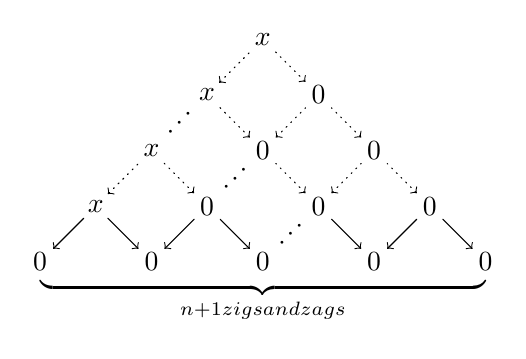
\begin{tikzpicture}[x=0.707cm,y=0.707cm,line cap=round]
			\node[inner sep=2] (00) at (0,0) {$0$};
			\node[inner sep=2] (01) at (2,0) {$0$};
			\node[inner sep=2] (02) at (4,0) {$0$};
			\node[inner sep=2] (03) at (6,0) {$0$};
			\node[inner sep=2] (04) at (8,0) {$0$};
			\node[inner sep=2] (10) at (1,1) {$x$};
			\node[inner sep=2] (11) at (3,1) {$0$};
			\node[inner sep=2] (12) at (5,1) {$0$};
			\node[inner sep=2] (13) at (7,1) {$0$};
			\node[inner sep=2] (20) at (2,2) {$x$};
			\node[inner sep=2] (21) at (4,2) {$0$};
			\node[inner sep=2] (22) at (6,2) {$0$};
			\node[inner sep=2] (30) at (3,3) {$x$};
			\node[inner sep=2] (31) at (5,3) {$0$};
			\node[inner sep=2] (40) at (4,4) {$x$};
			\draw[to-] (00) -- (10);
			\draw[to-] (01) -- (10);
			\draw[to-] (01) -- (11);
			\draw[to-] (02) -- (11);
			\draw[to-,dotted] (10) -- (20);
			\draw[to-,dotted] (11) -- (20);
			\draw[to-] (03) -- (12);
			\draw[to-,dotted] (12) -- (21);
			\draw[to-,dotted] (21) -- (30);
			\draw[to-] (04) -- (13);
			\draw[to-,dotted] (13) -- (22);
			\draw[to-,dotted] (22) -- (31);
			\draw[to-,dotted] (31) -- (40);
			\draw[to-] (03) -- (13);
			\draw[to-,dotted] (12) -- (22);
			\draw[to-,dotted] (21) -- (31);
			\draw[to-,dotted] (30) -- (40);
			\path (02) to  node[pos=0.5,sloped] {$\ldots$} (12);
			\path (11) to  node[pos=0.5,sloped] {$\ldots$} (21);
			\path (20) to  node[pos=0.5,sloped] {$\ldots$} (30);
			\node[rotate=-45] at (2,1) {$\pullbacksign$};
			\node[rotate=-45] at (6,1) {$\pullbacksign$};
			\node[rotate=-45] at (5,2) {$\pullbacksign$};
			\node[rotate=-45] at (4,3) {$\pullbacksign$};
			\path (00) to node[pos=0.5,below=0.5ex] {$\underbrace{\hspace{5.656cm}}_{n+1\text{ zigs and zags}}$} (04);
		\end{tikzpicture}
	\end{center}
	hence $\{0\}\times_{Q_n(\Cc)}\operatorname{Null}_n(\Cc)\simeq \Cc$. Moreover, $d_0\colon \operatorname{Null}_n(\Cc)\morphism Q_n(\Cc)$ is a split Verdier projection (with left/right Kan extension as adjoints, as usual), hence this pullback is preserved by $F$ and we obtain $\{0\}\times_{F(Q_n(\Cc))}F(\operatorname{Null}_n(\Cc))\simeq F(\Cc)$, as desired. This proves that we get a pullback diagram as above.
	
	If we can show that the right vertical arrow is equifibred, then we're done! Indeed, if this is the case, then \cref{lemdef:Equifibred} says that the diagram stays a pullback after applying $|\blank|\simeq \colimit_{\IDelta^\op}$. Hence we get a pullback
	\begin{equation*}
		\begin{tikzcd}
			\left|\const F(\Cc)\right|\rar\dar\drar[pullback] & \left|F\big(\operatorname{Null}(\Cc)\big)\right|\dar["\left|F(d_0)\right|"] \\
			\left|\const *\right|\rar["0"] & \left|F\big(Q(\Cc)\big)\right|
		\end{tikzcd}
	\end{equation*}
	The upper left corner is $F(\Cc)$, which coincides with the anima $\Hom_{\Span^F(\Cc)}(0,0)$ as argued in the proof of \cref{lem:GrouplikeFunctors}. The lower left corner is clearly $*$. Applying \cref{rem:Realisation} to 
	\begin{equation*}
		\asscat\big(F(\operatorname{Null}(\Cc))\big)\simeq 0/\Span^F(\Cc)\quad\text{and}\quad\asscat\big(F(Q(\Cc))\big)\simeq \Span^F(\Cc) 
	\end{equation*}
	shows that the upper and lower right corner coincide with $|0/\Span^F(\Cc)|\simeq *$ and $|\Span^F(\Cc)|$, hence the pullback diagram we get is precisely the one we want!
	
	It remains to show that $F(d_0)\colon F(\operatorname{Null}(\Cc))\morphism F(Q(\Cc))$ is equifibred. That is, we must show that
	\begin{equation*}
		\begin{tikzcd}
			F\big(\operatorname{Null}_m(\Cc)\big)\rar\dar\drar[pullback] & F\big(\operatorname{Null}_n(\Cc)\big)\dar\\
			F\big(Q_m(\Cc)\big) \rar & F\big(Q_n(\Cc)\big)
		\end{tikzcd}
	\end{equation*}
	is a pullback for every map $[m]\morphism{} [n]$ in $\IDelta^\op$. I think the way we did this in the lecture is too complicated and I can give a simpler proof. It seems almost too easy, so I feel a bit like I'm overlooking something, but I couldn't find anything. Please tell me if I'm wrong. 
	
	We've seen above that $\operatorname{Null}_n(\Cc)\morphism Q_n(\Cc)$ is a split Verdier projection with fibre $\Cc$, and so is $\operatorname{Null}_m(\Cc)\morphism Q_m(\Cc)$. Hence the induced map on fibres over $0$ in the diagram above is an equivalence, namely the identity on $F(\Cc)$. But that's enough to show the pullback property: Since $F$ is grouplike, all terms in the diagram are $\IE_\infty$-groups, hence all fibres are empty or equivalent to the fibres over $0$. But \cref{par:MoreOnVerdierSequences}\itememph{d^*} implies $F(\operatorname{Null}_n(\Cc))\simeq F(Q_n(\Cc))\times F(\Cc)$, and likewise $F(\operatorname{Null}_m(\Cc))\simeq F(Q_m(\Cc))\times F(\Cc)$, so none of the fibres can be empty. In fact, I believe the map $F(\operatorname{Null}_m(\Cc))\morphism F(\operatorname{Null}_n(\Cc))$ is the product map, which would make the pullback property even more apparent, but in any case the argument given above should suffice.
	%In fact, it suffices to consider maps in $\IDelta^\op_\mathrm{inj}$, since the realisation of a simplicial anima coincides with its realisation as a semi-simplicial anima (see the proof of \cref{lem:SkeletalInduction}), so we can replace $F(\operatorname{Null}(\Cc))$ and $F(Q(\Cc))$ as well as $\const F(\Cc)$ and $\const *$ with their semi-simplicial restrictions. Moreover, since $F(\operatorname{Null}(\Cc))$ and $F(Q(\Cc))$ satisfy the Segal conditions, it's enough to check the pullback property for the three maps $d_0,d_1,d_2\colon [2]\morphism{} [1]$ in $\IDelta^\op_\mathrm{inj}$. For $d_1$ and $d_2$, the would-be pullback squares are split Verdier squares before applying $F$, hence they stay pullback squares. For $d_0$ instead, we get a diagram
	%\begin{equation*}
	%	\begin{tikzcd}
	%		\operatorname{Null}_2(\Cc)\rar\dar & 	\operatorname{Null}_1(\Cc)\dar\\
	%		Q_2(\Cc) \rar & Q_n(\Cc)
	%	\end{tikzcd}
	%\end{equation*}
	%whose horizontal (!) maps are split Verdier projections (for $\operatorname{Null}_2(\Cc)\morphism\operatorname{Null}_1(\Cc)$ this needs a bit of fiddling, since we can't just take Kan extensions as always, but it's not hard to write down the adjoints explicitly), but this diagram is not a pullback.
\end{proof}

\begin{rem}\lecture[The relative $Q$-construction. Verdier quotients. Waldhausen's fibration theorem. Some final remarks on Karoubi sequences, inductive completions, Quillen's dévissage, and non-connective $K$-theory.\newline --- \emph{\enquote{What is the original formulation of Waldhausen's fibration theorem \dotso and where's the fibration?} \enquote{I never understood that.}}]{2021-02-11}\label{rem:RandomComment}
	Fabian started the final lecture with two not-so-random and one very random comment:
	\begin{alphanumerate}
		\item We know from \cref{lem:GrouplikeFunctors} and \cref{thm:Additivity} that $BF\simeq \Span^F(-)\simeq |\Span^F(-)|$ is additive again whenever $F$ is a grouplike additive functor. In fact, $BF$ is even grouplike by \cref{cor:CommutativeHorizontalAdjoints}\itememph{b}. More generally, it is true that $|\Span^F(-)|\simeq |F(Q(-))|$ is grouplike for any additive functor $F$, since $\pi_0|F(Q(-))|=0$ as seen in the proof of \cref{lem:GrouplikeFunctors}. However, if $F$ isn't grouplike, then $BF$ doesn't even need to be additive anymore, let alone coincide with $|F(Q(-))|$.
		\item Quillen defined $k(R)\coloneqq K_0(R)\times B\!\GL_\infty(R)^+$ and then showed a posteriori that it is an infinite loop space, essentially\footnote{Quillen did not put $\Dd^\perf(R)$ there, but still that's basically what he proved.} by verifying
		\begin{equation*}
			k(R)\simeq \Omega^i\big|\core Q^{i}\big(\Dd^\perf(R)\big)\big|\,.
		\end{equation*}
		Here $Q^{i}\colon \Catst\morphism \Fun((\IDelta^\op)^i,\Catst)$ denotes the $i$-fold $Q$-construction. It takes values in \enquote{$i$-simplicial} anima, and subsequently the realisation $|\blank|$ in the formula above doesn't denote colimits over $\IDelta^\op$, but over $(\IDelta^\op)^i$. 
		
		In the script \cite[Chapter~IV p.\:53]{KTheory}, Fabian explains a bit more. In general, if $F$ is an additive functor, then
		\begin{equation*}
			\Omega\left|F\big(Q(-)\big)\right|\simeq \Omega^i\left|F\big(Q^i(-)\big)\right|\,,
		\end{equation*}
		where again $|\blank|$ on the right-hand side denotes the colimit over $(\IDelta^\op)^i$. If $F$ is grouplike, then both sides are also equivalent to $F$. To prove the equivalence above, we use \cref{thm:Additivity} iteratively (along with \cref{cor:ColimitsCommute} to replace nested colimits over $\IDelta^\op$ by colimits over $(\IDelta^\op)^i$) to see that $|F(Q^i(-))|$ is additive. By the same argument as in \itememph{a}, it is also grouplike. Hence \cref{thm:SpanF} implies $|F(Q^i(-))|\simeq \Omega|F(Q^{i+1}(-))|$, from which the formula above follows by induction.
		
		Therefore, any additive functor $F\colon \Catst\morphism \An$ upgrades to a prespectra-valued (see \cref{par:Prespectra}) functor
		\begin{equation*}
			\operatorname{\IS pan}^F\colon \Catst\morphism \cat{PSp}
		\end{equation*}
		given by $\operatorname{\IS pan}^F(\Cc)\simeq (F(\Cc),\Omega |F(Q(\Cc))|,\Omega^2|F(Q^2(\Cc))|,\dotsc)$. The construction of $\operatorname{\IS pan}^F$ is clearly functorial in $F$, hence induces a functor
		\begin{equation*}
			\operatorname{\IS pan}^{(-)}\colon \Fun^\add(\Catst,\An)\morphism \Fun(\Catst,\cat{PSp})\,.
		\end{equation*}
		If we restrict to $\Fun^\grp(\Catst,\An)\subseteq \Fun^\add(\Catst,\An)$, then $\operatorname{\IS pan}^{(-)}$ takes values in $\Fun(\Catst,\Sp)$. Moreover, it follows from \itememph{a} that $\operatorname{\IS pan}^{(-)}$ coincides with $B^\infty$ on grouplike functors. Thus, for a stable $\infty$-category $\Cc$, we put
		\begin{equation*}
			K(\Cc)\coloneqq \operatorname{\IS pan}^{k}(\Cc)\simeq B^\infty k(\Cc)
		\end{equation*}
		and call this the \emph{$K$-theory spectrum} or \emph{projective class spectrum} of $\Cc$.
		\item Now for the random comment: If $\Sp_{[0,1]}\subseteq \Sp$ denotes the full subcategory of spectra $E$ whose homotopy groups $\pi_i(E)$ vanish for $i\notin[0,1]$, then 
		\begin{equation*}
			\Sp_{[0,1]}\simeq \CGrp(\An)_{[0,1]}\simeq \CGrp(\Grpd)\,.
		\end{equation*}
		A symmetric monoidal $1$-groupoid $\Gg^\otimes$ on the right-hand side corresponds to a gem (\enquote{generalised Eilenberg--MacLane anima}, see Very Long Example~\cref{exm:EilenberMacLane}) in the middle iff the symmetry isomorphisms $\sigma_{x,x}\colon x\otimes x\isomorphism x\otimes x$ from \labelcref{par:EinftyRefinement} is the identity on $x\otimes x$ for all $x\in \Gg$.
	\end{alphanumerate}
\end{rem}
\subsection{The Fibration Theorem}
To get fibre sequences like in \cref{par:SomeMotivation}, it doesn't suffice to know that $K$-theory is additive. For example, if $R\morphism S$ is a derived localisation of ordinary rings (\cref{propdef:derivedLocalisation}), then $\Dd(S)\morphism \Dd(R)\morphism \Dd(R)^{S\mhyph\mathrm{tors}}$ is a split Verdier sequence by \cref{lem:LocalisationRecollement}, but this is no longer true if we restrict to $\Dd^\perf$ everywhere. Instead, we'll have to show that $k\colon \Catst\morphism \An$ is Verdier-localising (\cref{def:VerdierStuff}), which is our next goal. It will turn out that even being Verdier-localising isn't quite enough, but more on that once we're there.
\begin{defi}\label{def:RelativeQ}
	If $f\colon \Aa\morphism\Bb$ is an exact functor of stable $\infty$-categories, then the \emph{relative $Q$-construction} $Q(f)\in \cat{sCat}_\infty^\mathrm{st}$ is defined by the pullback
	\begin{equation*}
		\begin{tikzcd}
			Q(f)\rar\dar\drar[pullback] & \operatorname{Null}(\Bb)\dar["d_0"] \\
			Q(\Aa)\rar["f"] & Q(\Bb)
		\end{tikzcd}
	\end{equation*}
\end{defi}
By \cref{par:MoreOnVerdierSequences}\itememph{e}, it doesn't matter whether this pullback is taken in $\cat{sCat}_\infty^\mathrm{st}$ or on $\cat{sCat}_\infty$. We may think of $Q_n(f)$ as diagrams of the following form (as usual, the dotted part is uniquely determined by the solid part):
\begin{center}
	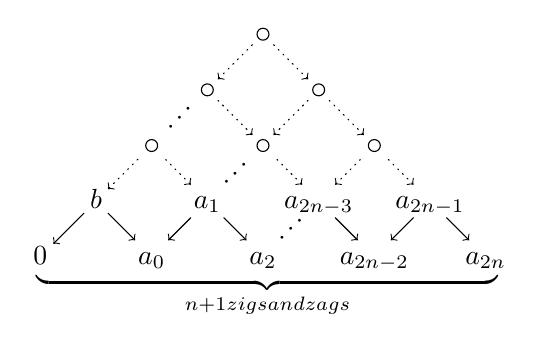
\begin{tikzpicture}[x=0.707cm,y=0.707cm,line cap=round]
		\node[text height=1.5ex,text depth=0.25ex,inner sep=2] (00) at (0,0) {$0$};
		\node[text height=1.5ex,text depth=0.25ex,inner sep=2] (01) at (2,0) {$a_0$};
		\node[text height=1.5ex,text depth=0.25ex,inner sep=2] (02) at (4,0) {$a_2$};
		\node[text height=1.5ex,text depth=0.25ex,inner sep=2] (03) at (6,0) {$a_{2n-2}$};
		\node[text height=1.5ex,text depth=0.25ex,inner sep=2] (04) at (8,0) {$a_{2n}$};
		\node[text height=1.5ex,text depth=0.25ex,inner sep=2] (10) at (1,1) {$b$};
		\node[text height=1.5ex,text depth=0.25ex,inner sep=2] (11) at (3,1) {$a_1$};
		\node[text height=1.5ex,text depth=0.25ex,inner sep=2] (12) at (5,1) {$a_{2n-3}$};
		\node[text height=1.5ex,text depth=0.25ex,inner sep=2] (13) at (7,1) {$a_{2n-1}$};
		\draw[fill=white] (2,2) circle (0.5ex) coordinate (20);
		\draw[fill=white] (4,2) circle (0.5ex) coordinate (21);
		\draw[fill=white] (6,2) circle (0.5ex) coordinate (22);
		\draw[fill=white] (3,3) circle (0.5ex) coordinate (30);
		\draw[fill=white] (5,3) circle (0.5ex) coordinate (31);
		\draw[fill=white] (4,4) circle (0.5ex) coordinate (40);
		\draw[to-] (00) -- (10);
		\draw[to-] (01) -- (10);
		\draw[to-] (01) -- (11);
		\draw[to-] (02) -- (11);
		\draw[to-,shorten >=1.25ex,dotted] (10) -- (20);
		\draw[to-,shorten >=1.25ex,dotted] (11) -- (20);
		\draw[to-] (03) -- (12);
		\draw[to-,shorten >=1.25ex,dotted] (12) -- (21);
		\draw[to-,shorten <=1.25ex,shorten >=1.25ex,dotted] (21) -- (30);
		\draw[to-] (04) -- (13);
		\draw[to-,shorten >=1.25ex,dotted] (13) -- (22);
		\draw[to-,shorten <=1.25ex,shorten >=1.25ex,dotted] (22) -- (31);
		\draw[to-,shorten <=1.25ex,shorten >=1.25ex,dotted] (31) -- (40);
		\draw[to-] (03) -- (13);
		\draw[to-,shorten >=1.25ex,dotted] (12) -- (22);
		\draw[to-,shorten <=1.25ex,shorten >=1.25ex,dotted] (21) -- (31);
		\draw[to-,shorten <=1.25ex,shorten >=1.25ex,dotted] (30) -- (40);
		\path (02) to  node[pos=0.5,sloped] {$\ldots$} (12);
		\path (11.center) to  node[pos=0.5,sloped] {$\ldots$} (21);
		\path (20.center) to  node[pos=0.5,sloped] {$\ldots$} (30);
		%\node[rotate=-45] at (2,1) {$\pullbacksign$};
		%\node[rotate=-45] at (6,1) {$\pullbacksign$};
		%\node[rotate=-45] at (5,2) {$\pullbacksign$};
		%\node[rotate=-45] at (4,3) {$\pullbacksign$};
		\path (00.center) to node[pos=0.51,below=0.5ex] {$\underbrace{\hspace{5.856cm}}_{n+1\text{ zigs and zags}}$} (04.center);
	\end{tikzpicture}
\end{center}
Here $a_0,\dotsc,a_{2n}\in \Aa$, $b\in \Bb$, and of course the arrow $b\morphism a_0$ should be interpreted as a morphism $b\morphism f(a_0)$ in $\Bb$.
\begin{cor}\label{cor:RelativeQ}
	If $F\colon \Catst\morphism \An$ is grouplike additive, then for all exact functors $f\colon \Aa\morphism \Bb$ there is a fibre sequence
	\begin{equation*}
		\left|F\big(Q(f)\big)\right|\morphism \left|F\big(Q(\Aa)\big)\right|\morphism \left|F\big(Q(\Bb)\big)\right|
	\end{equation*}
	in $\An$ \embrace{or equivalently in $\CGrp(\An)$}.
\end{cor}
\begin{proof}
	Recall the following facts from the second proof of \cref{thm:SpanF}:
	\begin{alphanumerate}
		\item $d_0\colon \operatorname{Null}_n(\Bb)\morphism Q_n(\Bb)$ is a split Verdier projection for all $[n]\in \IDelta^\op$; see Step~\itememph{2}.
		\item $F(d_0)\colon F(\operatorname{Null}(\Bb))\morphism F(Q(\Bb))$ is equifibred; see Step~\itememph{2}.
		\item $|F(\operatorname{Null}(\Bb))|\simeq |0/\Span^F(\Bb)|\simeq *$; see Step~\itememph{1}.
	\end{alphanumerate}
	By \itememph{a}, the pullback square defining $Q(f)$ is a degreewise split Verdier square. Hence it stays a pullback after applying $F$. Now \itememph{b} together with \cref{lemdef:Equifibred} ensures that we still get a pullback after taking realisations. By \itememph{c}, this pullback square provides the desired fibre sequence. 
\end{proof}
\begin{cor}\label{cor:GrouplikeVerdierLocalising}
	For a grouplike additive functor $F\colon \Catst\morphism \An$, the following are equivalent:
	\begin{alphanumerate}
		\item $F$ is Verdier-localising and sends Verdier projections to $\pi_0$-surjections. That is, for all Verdier-projections $\Bb\morphism \Cc$, the induced map $\pi_0(F(\Bb))\morphism \pi_0(F(\Cc))$ is surjective.
		\item For all Verdier inclusions $i\colon \Aa\morphism\Bb$ the canonical map
		\begin{equation*}
			\left|F\big(Q(i)\big)\right|\isomorphism F(\Bb/\Aa)
		\end{equation*}
		is an equivalence.
		\item[\itememph{c^*}] The functor $B^\infty F\colon \Catst\morphism \Sp$ is Verdier-localising.
	\end{alphanumerate}
\end{cor}
In the lecture, we only had \itememph{a} and \itememph{b}, and we didn't impose the condition that $F$ sends Verdier projections to $\pi_0$-surjections. I think it is needed though. In view of \itememph{\boxtimes} below, it's a natural question whether one can drop this condition (along with \itememph{c^*}) and in turn only ask for $\left|F(Q(i))\right|\morphism F(\Bb/\Aa)$ to be an inclusion of path components. However, I believe this breaks the argument why $F$ sends Verdier squares to pullbacks. Please tell me if it's true after all.

Also note that $K$-theory does send Verdier projections to $\pi_0$-surjections, which is clear from \cref{def:K0C} and the fact that $\Bb\morphism \Bb/\Aa$ is essentially surjective.
\begin{proof*}[Proof of \cref{cor:GrouplikeVerdierLocalising}]
	Let's first explain where the canonical map comes from. So for the moment, $F$ is only grouplike additive. \cref{thm:SpanF} implies $\Omega |F(Q(\Aa))|\simeq F(\Aa)$ and likewise for $\Bb$. Thus, rotating the fibre sequence from \cref{cor:RelativeQ} gives a fibre sequence
	\begin{equation*}
		F(\Aa)\morphism F(\Bb)\morphism \left|F\big(Q(i)\big)\right|
	\end{equation*}
	in $\CGrp(\An)$. We claim:
	\begin{alphanumerate}
		\item[\itememph{\boxtimes}] \itshape The induced map $\pi_0(F(\Bb))\morphism \pi_0\left|F(Q(i))\right|$ is surjective and thus the sequence above is also a fibre/cofibre sequence in $\Sp$.
	\end{alphanumerate}
	If $C$ denotes the cofibre in $\Sp$, then by \cref{lem*:WhiteheadForSpectra} it suffices to show that the canonical map $C\morphism \left|F(Q(i))\right|$ induces isomorphisms on all homotopy groups. Observe that $C$ is connective, so this holds for all negative homotopy groups, and the usual five lemma arguments show the same for all positive homotopy groups. It remains to check that $\pi_0(C)\morphism \pi_0\left|F(Q(i))\right|$ is an isomorphism. For that, we must show that $\pi_0(F(\Bb))\morphism \pi_0\left|F(Q(i))\right|$ is surjective. By \cref{lem:GrouplikeFunctors}, the fibre sequence from \cref{cor:RelativeQ} can be rewritten as
	\begin{equation*}
		\left|F\big(Q(i)\big)\right|\morphism BF(\Aa)\morphism BF(\Bb)\,.
	\end{equation*}
	Hence $\pi_1(BF(\Bb))\morphism \pi_0\left|F(Q(i))\right|\morphism \pi_0(BF(\Aa))$ is exact. But $\pi_1(BF(\Bb))=\pi_0(F(\Bb))$ and $\pi_0(BF(\Aa))=0$ since $B$ shifts homotopy groups up. Thus $\pi_0(F(\Bb))\morphism \pi_0\left|F(Q(i))\right|$ is indeed surjective and we've proved \itememph{\boxtimes}.
	
	Now for the actual proof. Since $F(\Aa)\morphism F(\Bb)\morphism F(\Bb/\Aa)$ always composes to $0$, \itememph{\boxtimes} provides the desired natural map $\left|F(Q(i))\right|\morphism F(\Bb/\Aa)$. Assume \itememph{a} holds. Then $F(\Aa)\morphism F(\Bb)\morphism F(\Bb/\Aa)$ is a fibre sequence too. By the usual five lemma arguments, $\left|F(Q(i))\right|\morphism F(\Bb/\Aa)$ is an isomorphism on all homotopy groups except possibly $\pi_0$. But since $\pi_0(F(\Bb))\morphism \pi_0(F(\Bb/\Aa))$ is surjective by assumption and $\pi_0(F(\Bb))\morphism \pi_0\left|F(Q(i))\right|$ is surjective by \itememph{\boxtimes}, the five lemma also works in $\pi_0$. This shows \itememph{a} $\Rightarrow$ \itememph{b}.
	
	Conversely, assume that $\left|F(Q(i))\right|\isomorphism F(\Bb/\Aa)$. Then $F$ sends Verdier sequences to fibre sequences and Verdier projections to $\pi_0$-surjections. It remains to show that $F$ transforms Verdier squares into pullbacks. But whether a square in $\CGrp(\An)$ is a pullback square can be tested on fibres. Since $F$ sends Verdier projections to $\pi_0$-surjections, all fibres are non-empty and thus all fibres are equivalent to the respective fibres over $0$. But the induced map on fibres over $0$ is an equivalence since we know what $F$ does on Verdier sequences. This shows \itememph{b} $\Rightarrow$ \itememph{a}.
	
	Finally, for \itememph{a} $\Leftrightarrow$ \itememph{c^*} it suffices to observe that a fibre sequence $X\morphism Y\morphism Z$ in $\CGrp(\An)$ stays a fibre sequence under $B^\infty\colon \CGrp(\An)\morphism \Sp$ iff $\pi_0(Y)\morphism \pi_0(Z)$ is surjective, which follows from the argument in \itememph{\boxtimes}.
\end{proof*}
We still owe a proof that cofibres in $\Catst$ can be described as in \labelcref{par:CofibreSequencesInCatSt}. The following takes care of the essential case.
\begin{lem}\label{lem:VerdierQuotients}
	Let $\Cc\subseteq \Dd$ be a stable sub-$\infty$-category \embrace{in the sense of \cref{warn*:StableSubcategory}} and let $\Dd/\Cc$ be the localisation of $\Dd$ at the mod-$\Cc$ equivalences. Then for all $x,y\in\Dd$,
	\begin{equation*}
		\Hom_{\Dd/\Cc}(x,y)\simeq\colimit_{c\in\Cc/y}\Hom_\Dd\big(x,\cofib(c\rightarrow y)\big)\,.
	\end{equation*}
	In particular, $\Dd/\Cc$ is stable and $\Dd\morphism \Dd/\Cc$ is an exact functor.
\end{lem}
\cref{lem:VerdierQuotients} only takes care of the fully faithful case, but it follows at once that the description from \labelcref{par:CofibreSequencesInCatSt} also holds for arbitrary exact functors. Moreover, note that the slice category $\Cc/y\coloneqq \Cc\times_\Dd\Dd/y$ is filtered. Indeed, given any map $K\morphism \Cc/y$ from a finite simplicial set $K$, we can find an extension $K^\triangleright\morphism \Cc/y$ by taking the colimit in $\Cc$, which maps canonically to $y$ since $\Cc\subseteq \Dd$ preserves finite colimits. Moreover, recall that filtered colimits in $\An$ commute with finite limits. This is proved in \cite[Proposition~\HTTthm{5.3.3.3}]{HTT}, but I think it also follows from \cref{rem*:piPreservesFilteredColimits} after some fiddling.
\begin{proof}[Proof of \cref{lem:VerdierQuotients}]
	Let $W\subseteq \pi_0\core\Ar(\Dd)$ be the collection of morphisms whose fibre is in $\Cc$. In the definition of mod-$\Cc$ equivalences we also allowed morphisms whose fibre is only a retract of an object of $\Cc$, but once we've shown that $\Dd[W^{-1}]$ is stable and $p\colon \Dd\morphism \Dd[W^{-1}]$ is exact, it will be clear that $\Dd[W^{-1}]$ coincides with the localisation $\Dd/\Cc$ at all mod-$\Cc$ equivalences.
	
	Recall from \cref{lem:HomsInLocalisation} that $\Hom_{\Dd[W^{-1}]}(x,-)\colon \Dd[W^{-1}]\morphism \An$ is left-Kan extended from $\Hom_\Dd(x,-)\colon \Dd\morphism \An$. Moreover, left Kan extension $p_!$ sits in an adjunction
	\begin{equation*}
		p_!\colon \Fun(\Dd,\An)\doublelrmorphism \Fun\big(\Dd[W^{-1}],\An\big)\noloc p^*
	\end{equation*}
	in which $p^*$ is fully faithful. Hence $p^*p_!\colon \Fun(\Dd,\An)\morphism \Fun(\Dd,\An)$ defines a left Bousfield localisation onto the full sub-$\infty$-category of functors that invert $W$.
	
	The idea is now to guess an explicit description of $p^*p_!$ and verify its correctness using Proposition~\labelcref{prop:LLaddendum}. Consider the functor $L\colon \Fun(\Dd,\An)\morphism \Fun(\Dd,\An)$ defined by
	\begin{equation*}
		LF(x)\simeq \colimit_{c\in \Cc/x}F\big(\cofib(c\rightarrow x)\big)\,.
	\end{equation*}
	The functorial maps $x\morphism \cofib(c\morphism x)$ define a map 
	\begin{equation*}
		F(x)\simeq \colimit_{c\in\Cc/x}F(x)\morphism \colimit_{c\in\Cc/x}F\big(\cofib(c\rightarrow x)\big)\,,
	\end{equation*}
	where the equivalence on the left follows from the fact that any filtered $\infty$-category is weakly contractible. One checks that these maps are functorial in $x$ and $F$, whence they assemble into a natural transformation $\eta\colon\id\Rightarrow L$. We claim:
	\begin{numerate}\itshape
		\item For all $F$, the functor $LF$ inverts $W$.
		\item If $F$ already inverts $W$, then $\eta\colon F\morphism LF$ is an equivalence.
	\end{numerate}
	Claims~\itememph{1} and \itememph{2} together easily imply that the conditions of Proposition~\labelcref{prop:LLaddendum} are met, so indeed $L\simeq p^*p_!$. This also proves that $\Hom$ anima in $\Dd[W^{-1}]$ are given by
	\begin{equation*}
		\Hom_{\Dd[W^{-1}]}(x,y)\simeq \colimit_{c\in\Cc/y}\Hom_\Dd\big(x,\cofib(c\rightarrow y)\big)\,.
	\end{equation*}
	Using this formula together with \cref{cor:HomPreservesColimits} and the fact that filtered colimits commute with finite limits shows that $\Dd\morphism \Dd[W^{-1}]$ preserves finite colimits. Using the same argument for $\Dd^\op\morphism \Dd^\op[(W^\op)^{-1}]$ shows that $\Dd\morphism \Dd[W^{-1}]$ also preserves finite limits. Moreover, we can get that $\Dd[W^{-1}]$ has finite limits out of this. We already have a terminal object, hence it suffices to have pullbacks. But every span $x\morphism y\lmorphism z$ in $\Dd[W^{-1}]$ can be represented by a span $x\morphism \cofib(c\morphism y)\lmorphism z$ in $\Dd$ for some $c\in\Cc/y$, since the colimit in the formula above is filtered. Now $y\morphism \cofib(c\morphism y)$ is in $W$, hence an equivalence in $\Dd[W^{-1}]$, thus it suffices to take the pullback in $\Dd$ to get the desired pullback in $\Dd[W^{-1}]$. In the same way, one shows that $\Dd[W^{-1}]$ has finite colimits. Moreover, our argument also shows that pullback and pushout squares coincide, whence $\Dd[W^{-1}]$ is stable by \cref{propdef:StableInftyCategory}\itememph{c}. This proves everything we want, safe for the two claims above.
	
	We didn't prove these claims in the lecture, but here's what I think should work. Let's first check \itememph{1}. Suppose $\phi\colon x\morphism y$ has fibre in $\Cc$. Then also $\cofib(x\morphism y)\in \Cc$. Now, for any $c\in \Cc/y$, consider the following diagram:
	\begin{equation*}
		\begin{tikzcd}[column sep=small]
			\phi^*c\dar\drar[pullback]\rar & x\dar["\phi"] \rar\drar[pullback] & 0\dar\\
			c \rar\dar\drar[pullback] & y\dar\rar & \cofib(x\morphism y)\\
			0 \rar & \cofib(c\morphism y)
		\end{tikzcd}
	\end{equation*}
	From the upper two squares we obtain that $\phi^*c\morphism c\morphism \cofib(x\morphism y)$ is a fibre sequence in $\Dd$, two of whose terms are in $\Cc$. Hence also $\phi^*c\in \Cc$. Thus, taking pullbacks along $\phi$ defines a functor $\phi^*\colon \Cc/y\morphism \Cc/x$, which one readily checks to be right-adjoint to the forgetful functor $\phi_!\colon \Cc/x\morphism \Cc/y$. Recall that right adjoints are cofinal; see the discussion after \cref{def:cofinal}. Moreover, the left two squares in the diagram above show $\cofib(\phi^*c\morphism x)\simeq \cofib(c\morphism y)$. Hence $\phi^*$ defines an equivalence
	\begin{equation*}
		\phi^*\colon LF(y)\simeq \colimit_{c\in\Cc/y}F\big(\cofib(\phi^*c\rightarrow x)\big)\isomorphism \colimit_{c'\in \Cc/x}F\big(\cofib(c'\rightarrow x)\big)\simeq LF(x)\,.
	\end{equation*}
	One checks that $\phi^*$ is an inverse to the induced map $LF(\phi)\colon LF(x)\morphism LF(y)$, so that $LF$ indeed inverts $W$. This shows \itememph{1}.
	
	It remains to show \itememph{2}, which is easy: $x\morphism \cofib(c\morphism x)$ lies in $W$ because its fibre is $c$. Hence $F(x)\isomorphism F(\cofib(c\morphism x))$ is an equivalence, which proves that $F(x)\isomorphism LF(x)$ is an equivalence as well for all $x\in \Dd$.
\end{proof}
To prove that $K$-theory is Verdier-localising, we invoke a somewhat non-standard formulation of Waldhausen's fibration theorem.
\begin{thm}[Waldhausen's fibration theorem]\label{thm:Fibration}
	Let $\Aa\subseteq \Bb$ be a stable sub-$\infty$-category, let $K$ be a finite $\infty$-category, and let $\Fun^\Aa(K,\Bb)\subseteq \Fun(K,\Bb)$ be the wide sub-$\infty$-category spanned by all objects but only the pointwise mod-$\Aa$ equivalences. Then
	\begin{equation*}
		\big|\Fun^\Aa(K,\Bb)\big|\morphism \Fun(K,\Bb/\Aa)
	\end{equation*}
	is \emph{faithful}, i.e., it induces inclusions of path components on $\Hom$ anima. Furthermore:
	\begin{alphanumerate}
		\item If $\Aa\subseteq \Bb$ is a Verdier inclusion \embrace{i.e.\ closed under retracts}, then the map above is an equivalence onto $\core \Fun(K,\Bb/\Aa)$.
		\item If $\Aa\subseteq \Bb$ is dense, then $|\Fun^\Aa(K,\Bb)|$ is discrete \embrace{since $\Bb/\Aa\simeq 0$}. In fact, it is the discrete group $K_0\Fun(K,\Bb)/K_0\Fun(K,\Aa)$.
	\end{alphanumerate}
\end{thm}

\noindent\begin{tikzpicture}[line cap=round,line join=round]
	\node[text width=\textwidth,inner sep=0,align=justify,below] {\emph{Proof.}};
	\node[text width=\textwidth,inner sep=0,align=justify,below] at (0,-9\baselineskip) {\phantom{Toast}\qed};
	\begin{scope}[opacity=0.25,black!12!white]
		\node[text width=\textwidth,inner sep=0,align=justify,below] at (0,0) {\phantom{\emph{Proof.}} \contour{black!20!white}{Lorem ipsum dolor sit amet, consectetuer adipiscing elit.} \contour{black!20!white}{Ut purus elit, vestibulum} \phantom{ut, placerat ac,}};
		
		\node[text width=\textwidth,inner sep=0,align=justify,below] at (0,-\baselineskip) {\contour{black!20!white}{ut, placerat ac, adispiscing vitae, felis.} \contour{black!20!white}{Curabitur dictum gravida mauris. Nam arcu libero} \phantom{nonnummy}};
		
		\node[text width=\textwidth,inner sep=0,align=justify,below] at (0,-2\baselineskip) {\contour{black!20!white}{nonummy eget, consectetuer id, vulputate a, magna.}\hfill \contour{black!20!white}{Donec vehicula augue eu neque. Pel-}};
		
		\node[text width=\textwidth,inner sep=0,align=justify,below] at (0,-3\baselineskip) {\contour{black!20!white}{lentesque habitant morbi tristique}\hfill \contour{black!20!white}{senectus et netus et malesuada fames ac turpis egestas.}};
		
		\node[text width=\textwidth,inner sep=0,align=justify,below] at (0,-4\baselineskip) {\contour{black!20!white}{Mauris ut leo. Cras viverra metus rhoncus sem.}\hfill \contour{black!20!white}{Nulla et lectus vestibulum urna fringilla}};
		
		\node[text width=\textwidth,inner sep=0,align=justify,below] at (0,-5\baselineskip) {\contour{black!20!white}{ultrices. Phasellus eu tellus sit amet tortor gravida placerat.}\hfill \contour{black!20!white}{Integer sapien est, iaculis in,}};
		
		\node[text width=\textwidth,inner sep=0,align=justify,below] at (0,-6\baselineskip) {\contour{black!20!white}{pretium quis, viverra ac, nunc.}\hfill \contour{black!20!white}{Praesent eget sem vel leo ultrices bibendum. Aenean fauci-}};
		
		\node[text width=\textwidth,inner sep=0,align=justify,below] at (0,-7\baselineskip) {\contour{black!20!white}{bus. Morbi dolor nulla, malesuada eu, pulvinar at, mollis ac, nulla.}\hfill \contour{black!20!white}{Curabitur auctor sem-}};
		
		\node[text width=\textwidth,inner sep=0,align=justify,below] at (0,-8\baselineskip) {\contour{black!20!white}{per nulla. Donec varius orci eget risus.} \contour{black!20!white}{Duis nibh mi congue eu, accumsan eleifend, saggitis} \phantom{quis, diam.}};
		
		\node[text width=\textwidth,inner sep=0,align=justify,below] at (0,-9\baselineskip) {\contour{black!20!white}{quis, diam. Duis eget orci sit amet orci dignissim rutrum.}};
	\end{scope}
	\draw[fill=white,rounded corners=2] (-3.7,-0.15) rectangle (3.7,-3.95);
	\sffamily
	\node[align=justify,text width=6cm] at (0,-0.62) {\footnotesize\textbf{This proof is part of Andrea's Master's Thesis}\\[-1ex]
		\scriptsize Please, select a purchase option:};
	\begin{scope}[yshift=0.05cm]
		\begin{scope}
			\clip[rounded corners=1] (-2.4,-1.06) rectangle (2.4,-3.4);
			\fill[black!20!white] (-2.4,-2.9) rectangle (2.4,-3.4);
		\end{scope}
		\draw[rounded corners=1] (-2.4,-1.06) rectangle (2.4,-3.4);
		\draw (-2.4,-2.9) -- (2.4,-2.9);
		\node[align=left,text width=4cm] at (0.2,-1.31) {\scriptsize Hardcover Book\hfill \textbf{\$99.99}};
		\node[align=left,text width=4cm,below] at (0.2,-1.35) {\hfill \tiny Price includes VAT};
		\node[align=left,text width=3.75cm,below] at (0.2,-1.6) {\scriptsize $\bullet$ Dispatched in about 6 Months\\[-1ex]
			$\bullet$ Free shipping worldwide};
		\fill[FabiansPurple!75!FabiansPink,rounded corners=1.5] (-1.8,-2.4) rectangle (2.2,-2.8);
		\node[white] at (0.2,-2.6) {\hypersetup{urlcolor=white}\scriptsize \textbf{\href{http://tiny.cc/AlgebraicHermitianKTheory}{Buy Hardcover Book}}};
		\node[align=left,text width=4cm] at (0.2,-3.15) {\scriptsize eBook\hfill \textbf{\$89.99}};
		\draw[shift={(-2.1,-1.31)},FabiansPurple!75!FabiansPink] (0,0) circle (0.6ex);
		\fill[shift={(-2.1,-1.31)},FabiansPurple!75!FabiansPink] (0,0) circle (0.35ex);
		\draw[shift={(-2.1,-3.15)},FabiansPurple!75!FabiansPink,fill=white] (0,0) circle (0.6ex);
	\end{scope}
	
	%\draw[shift={(-2.15,-1.3)},thick] (0,0) -- (0.5ex,-0.5ex) -- (1ex,0);
	%\draw[shift={(-2.15,-3.1)},thick] (0.5ex,-0.5ex) -- (1ex,0) -- (0.5ex,0.5ex);
	\node[align=right,text width=3cm,left] at (0,-3.7) {\hypersetup{urlcolor=black}\tiny\bfseries  \href{http://tiny.cc/AlgebraicHermitianKTheory}{\underline{Learn about $K$-Theor\smash{y} PREMIUM}}};
	\node[align=left,text width=3.2cm,right] at (0,-3.7) {\hypersetup{urlcolor=black}\tiny Already have an account? \href{http://tiny.cc/AlgebraicHermitianKTheory}{\underline{\textbf{Si\smash{g}n in}}}};;
	\draw (0,-3.5) -- (0,-3.8);
\end{tikzpicture}
\begin{cor}\label{cor:KVerdierLocalising}
	The $K$-Theory functor $k\colon \Catst\morphism \An$ is Verdier-localising. The same is true for its spectra-valued variant $K\simeq B^\infty k\colon \Catst\morphism \Sp$.
\end{cor}
\begin{proof}[Proof sketch]
	Let $i\colon \Aa\morphism \Bb$ be a Verdier inclusion. Consider the simplicial stable $\infty$-category
	\begin{equation*}
		\Fun(-,\Bb)\colon \IDelta^\op\morphism \Catst
	\end{equation*}
	sending $[n]\mapsto \Fun([n],\Bb)$. We claim that there is a degreewise fully faithful inclusion
	\begin{equation*}
		Q(i)\subseteq \Fun(-,\Bb)^\mathrm{esd}
	\end{equation*}
	(where $(-)^\mathrm{esd}$ denotes the edgewise subdivision; see \labelcref{par:edgewiseSubdivision}) with degreewise essential image those functors in $\Fun([n],\Bb)$ that land in the mod-$\Aa$ equivalences. To see this, recall that the elements of $Q_n(i)$ can be pictured as diagrams
	\begin{center}
		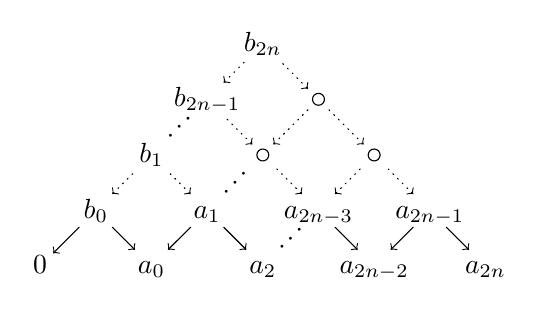
\begin{tikzpicture}[x=0.707cm,y=0.707cm,line cap=round]
			\node[text height=1.5ex,text depth=0.25ex,inner sep=2] (00) at (0,0) {$0$};
			\node[text height=1.5ex,text depth=0.25ex,inner sep=2] (01) at (2,0) {$a_0$};
			\node[text height=1.5ex,text depth=0.25ex,inner sep=2] (02) at (4,0) {$a_2$};
			\node[text height=1.5ex,text depth=0.25ex,inner sep=2] (03) at (6,0) {$a_{2n-2}$};
			\node[text height=1.5ex,text depth=0.25ex,inner sep=2] (04) at (8,0) {$a_{2n}$};
			\node[text height=1.5ex,text depth=0.25ex,inner sep=2] (10) at (1,1) {$b_0$};
			\node[text height=1.5ex,text depth=0.25ex,inner sep=2] (11) at (3,1) {$a_1$};
			\node[text height=1.5ex,text depth=0.25ex,inner sep=2] (12) at (5,1) {$a_{2n-3}$};
			\node[text height=1.5ex,text depth=0.25ex,inner sep=2] (13) at (7,1) {$a_{2n-1}$};
			\node[text height=1.5ex,text depth=0.25ex,inner sep=2] (20) at  (2,2) {$b_1$};
			\draw[fill=white] (4,2) circle (0.5ex) coordinate (21);
			\draw[fill=white] (6,2) circle (0.5ex) coordinate (22);
			\node[text height=1.5ex,text depth=0.25ex,inner sep=2] (30) at  (3,3) {$b_{2n-1}$};
			\draw[fill=white] (5,3) circle (0.5ex) coordinate (31);
			\node[text height=1.5ex,text depth=0.25ex,inner sep=2] (40) at  (4,4) {$b_{2n}$};
			\draw[to-] (00) -- (10);
			\draw[to-] (01) -- (10);
			\draw[to-] (01) -- (11);
			\draw[to-] (02) -- (11);
			\draw[to-,dotted] (10) -- (20);
			\draw[to-,dotted] (11) -- (20);
			\draw[to-] (03) -- (12);
			\draw[to-,shorten >=1.25ex,dotted] (12) -- (21);
			\draw[to-,shorten <=1.25ex,dotted] (21) -- (30);
			\draw[to-] (04) -- (13);
			\draw[to-,shorten >=1.25ex,dotted] (13) -- (22);
			\draw[to-,shorten <=1.25ex,shorten >=1.25ex,dotted] (22) -- (31);
			\draw[to-,shorten <=1.25ex,dotted] (31) -- (40);
			\draw[to-] (03) -- (13);
			\draw[to-,shorten >=1.25ex,dotted] (12) -- (22);
			\draw[to-,shorten <=1.25ex,shorten >=1.25ex,dotted] (21) -- (31);
			\draw[to-,dotted] (30) -- (40);
			\path (02) to  node[pos=0.5,sloped] {$\ldots$} (12);
			\path (11.center) to  node[pos=0.5,sloped] {$\ldots$} (21);
			\path (20.center) to  node[pos=0.5,sloped] {$\ldots$} (30.center);
			%\node[rotate=-45] at (2,1) {$\pullbacksign$};
			%\node[rotate=-45] at (6,1) {$\pullbacksign$};
			%\node[rotate=-45] at (5,2) {$\pullbacksign$};
			%\node[rotate=-45] at (4,3) {$\pullbacksign$};
			%\path (00.center) to node[pos=0.51,below=0.5ex] {$\underbrace{\hspace{5.856cm}}_{n+1\text{ zigs and zags}}$} (04.center);
		\end{tikzpicture}
	\end{center}
	where $a_0,\dotsc,a_{2n}\in \Aa$, $b_0\in \Bb$, and the $b_1,\dotsc,b_n$ as well as the rest of the diagram are uniquely determined by the pullback conditions. To such a diagram, we can associate the sequence
	\begin{equation*}
		\fib(b_0\rightarrow a_0)\morphism \dotso \morphism\fib(b_{2n}\rightarrow a_{2n})\morphism b_{2n}\morphism \dotso \morphism b_0\,,
	\end{equation*}
	which evidently is an element of $\Fun([2n+1],\Bb)\simeq (\Fun(-,\Bb)^\mathrm{esd})_n$, and one easily checks that all maps are actually mod-$\Aa$ equivalences. Conversely, the diagram can be uniquely reconstructed from the sequence. To make this precise, one should argue similar to \cref{prop:QvsS}, but we'll leave the details to you.
	
	We conclude that $Q_nQ_m(i)$ consists of functors $J_n\times[2m+1]\morphism \Bb$ that take all morphisms $(j,k)\morphism(j,\ell)$ to mod-$\Aa$ equivalences. Thus $Q_nQ_m(i)\simeq \Fun([2m+1],\Fun^\Aa(J_n,\Bb))$ and therefore
	\begin{equation*}
		\core Q_nQ(i)\simeq \big(\N^r\Fun^\Aa(J_n,\Bb)\big)^\mathrm{esd}\,.
	\end{equation*}
	Taking realisations and using \cref{thm:Fibration}\itememph{a}, we obtain
	\begin{equation*}
		\left|\core Q_nQ(i)\right|\simeq \big|\Fun^\Aa(J_n,\Bb)\big|\simeq \core \Fun(J_n,\Bb/\Aa)\,.
	\end{equation*}
	Combining this with \cref{lem:GrouplikeFunctors} shows
	\begin{equation*}
		\left|Bk\big(Q(i)\big)\right|\simeq  \left|\core Q\big(Q(i)\big)\right|\simeq \left|\core Q(\Bb/\Aa)\right|\simeq Bk(\Bb/\Aa)
	\end{equation*}
	(the second realisation is actually a colimit over $(\IDelta^\op)^2$, similar to \cref{rem:RandomComment}\itememph{b}). By \cref{cor:GrouplikeVerdierLocalising}, this shows that $Bk\colon \Catst\morphism \CGrp(\An)$ and $B^{\infty+1}k\colon \Catst\morphism \Sp$ are Verdier-localising. Hence so are $k\simeq \Omega Bk$ and $K\simeq B^\infty k\simeq (B^{\infty+1}k)[-1]$.
\end{proof}
\begin{cor}\label{cor:KDenseInclusion}
	If $\Aa\subseteq \Bb$ is a dense stable sub-$\infty$-category, then $K_i(\Aa)\isomorphism K_i(\Bb)$ is an isomorphism for all $i\geq 1$.
\end{cor}
\begin{proof*}
	Throughout the proof, let $i\colon \Aa\morphism \Bb$ denote the inclusion and let $A=K_0(\Bb)/K_0(\Aa)$. Recall from the proof of \cref{cor:GrouplikeVerdierLocalising} that there is a fibre sequence
	\begin{equation*}
		Bk(\Aa)\morphism Bk(\Bb)\morphism \left|Bk\big(Q(i)\big)\right|\,.
	\end{equation*}
	Since $B$ shifts homotopy groups up, the statement of the corollary is equivalent to $\left|Bk(Q(i))\right|$ being the Eilenberg--MacLane anima $K(A,1)$. As in the proof of \cref{cor:KVerdierLocalising}, but using \cref{thm:Fibration}\itememph{b} instead, we get
	\begin{equation*}
		\left|\core Q_nQ(i)\right|\simeq \big|\Fun^\Aa(J_n,\Bb)\big|\simeq K_0\Fun(J_n,\Bb)/K_0\Fun(J_n,\Aa)\,.
	\end{equation*}
	Now \cref{lem:GrouplikeFunctors} implies $K_0\Fun(J_n,\Bb)/K_0\Fun(J_n,\Aa)=A^{2n+1}$, and thus
	\begin{equation*}
		\left|Bk\big(Q(i)\big)\right|\simeq  \left|\core Q\big(Q(i)\big)\right|\simeq \colimit_{[n]\in \IDelta^\op}A^{2n+1}\,.
	\end{equation*}
	Be aware that the colimit on the right-hand side is taken in $\An$, regarding the abelian groups $A^{2n+1}$ as discrete anima, and thus the simplicial abelian group $A^{2\bullet+1}\colon \IDelta^\op\morphism \Ab$ as a discrete simplicial anima. Let's analyse the face maps in $A^{2\bullet+1}$. Elements of $\Fun(J_n,\Bb)$ are given by zigzags
		\begin{center}
		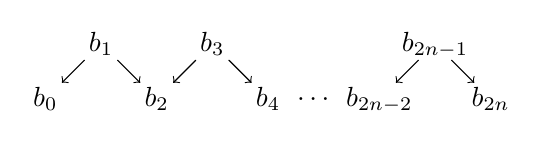
\begin{tikzpicture}[x=0.707cm,y=0.707cm,line cap=round]
			\node[text height=1.5ex,text depth=0.25ex,inner sep=2] (00) at (0,0) {$b_0$};
			\node[text height=1.5ex,text depth=0.25ex,inner sep=2] (01) at (2,0) {$b_2$};
			\node[text height=1.5ex,text depth=0.25ex,inner sep=2] (02) at (4,0) {$b_4$};
			\node[text height=1.5ex,text depth=0.25ex,inner sep=2] (03) at (6,0) {$b_{2n-2}$};
			\node[text height=1.5ex,text depth=0.25ex,inner sep=2] (04) at (8,0) {$b_{2n}$};
			\node[text height=1.5ex,text depth=0.25ex,inner sep=2] (10) at (1,1) {$b_1$};
			\node[text height=1.5ex,text depth=0.25ex,inner sep=2] (11) at (3,1) {$b_3$};
			\node[text height=1.5ex,text depth=0.25ex,inner sep=2] (13) at (7,1) {$b_{2n-1}$};
			\draw[to-] (00) -- (10);
			\draw[to-] (01) -- (10);
			\draw[to-] (01) -- (11);
			\draw[to-] (02) -- (11);
			\draw[to-] (04) -- (13);
			\draw[to-] (03) -- (13);
			\path (02) to  node[pos=0.5,sloped] {$\ldots$} (03);
		\end{tikzpicture}
	\end{center}
	for some $b_0,\dotsc,b_{2n}\in\Bb$. The outer face maps $d_0,d_{n}\colon \Fun(J_n,\Bb)\morphism \Fun(J_{n-1},\Bb)$ simply chop of $b_0$, $b_1$ or $b_{2n-1}$, $b_{2n}$, respectively. The inner face maps $d_j\colon \Fun(J_n,\Bb)\morphism \Fun(J_{n-1},\Bb)$ for $1\leq j<n$ remove $b_{2j-1}$, $b_{2j}$, $b_{2j+1}$ and replace them by the pullback $b_{2j-1}\times_{b_{2j}}b_{2j+1}$ in $\Bb$. Once we note that $[b_{2j-1}\times_{b_{2j}}b_{2j+1}]=[b_{2j-1}]+[b_{2j+1}]-[b_{2j}]$ in $K_0(\Bb)$, it follows that the face maps $d_j\colon A^{2n+1}\morphism A^{2n-1}$ in $A^{2\bullet+1}$ are given thusly:
	\begin{equation*}
		d_j(a_0,\dotsc,a_{2n})=
		\begin{cases*}
			(a_2,\dotsc,a_{2n}) & if $j=0$\\
			(a_0,\dotsc,a_{2j-2},a_{2j-1}+a_{2j+1}-a_{2j},a_{2j+2},\dotsc,a_{2n}) & if $1\leq j<n$\\
			(a_0,\dotsc,a_{2n-2}) & if $j=n$
		\end{cases*}\,.
	\end{equation*}
	The simplicial abelian group $A^{2\bullet+1}$ is a Kan complex by \cref{exm:MyFirstKanComplexes}\itememph{c}. Hence \cref{rem:Realisation} implies that $\colimit_{[n]\in\IDelta^\op}A^{2n+1}$ is just given by $A^{2\bullet+1}$ itself, considered as an anima. By \cref{thm:DoldKan}, the homotopy groups of $A^{2\bullet+1}$ are the homology groups of its normalised chain complex $N_*(A^{2\bullet+1})$, where $N_n(A^{2\bullet+1})=\bigcap_{1\leq j\leq n}\ker(d_j)\subseteq A^{2n+1}$ and the differentials are given by $d_0$. One easily checks $N_0(A^{2\bullet+1})=A$, $N_0(A^{2\bullet+1})=A^2$, and $N_n(A^{2\bullet+1})=0$ for $n\geq 2$, which upon inspection of the differentials shows that $A^{2\bullet+1}$ is indeed the Eilenberg--MacLane anima $K(A,1)$.
\end{proof*}
\subsection{Localisation and Dévissage}
\numpar{}\label{par:ThingsLeftToDo}
Two final things are left to do:
\begin{alphanumerate}
	\item If $R\morphism S$ is a derived localisation of rings (we will soon see how to generalise this to an arbitrary localisation of $\IE_\infty$-ring spectra), we wish to show that under a soon to be specified mild technical condition ($R\morphism S$ having \emph{perfectly generated fibre}) there is a fibre sequence
	\begin{equation*}
		k\big(\Dd^\perf(R)^{S\mhyph\mathrm{tors}}\big)\morphism k\big(\Dd^\perf(R)\big)\morphism k\big(\Dd^\perf(S)\big)\,.
	\end{equation*}
	This is not yet trivial since \cref{cor:KVerdierLocalising} isn't applicable right away: Even though $\Dd(R)^{S\mhyph\mathrm{tors}}\morphism \Dd(R)\morphism \Dd(S)$ is a Verdier sequence by \cref{lem:LocalisationRecollement} and \cref{thm:VerdierStuff}, the same need not be true anymore after restricting to the full sub-$\infty$-categories of perfect complexes everywhere. For example, $S\otimes_R-\colon \Dd^\perf(R)\morphism \Dd^\perf(S)$ may fail to be essentially surjective. This can already be the case for $S\otimes_R-\colon \Proj(R)\morphism \Proj(S)$. However, its essential image is always a dense subcategory, since every finite free $S$-module is hit and every finite projective $S$-module is a retract of a finite free one. This observation leads us on the right track, as we'll see in a moment.
	\item If $R$ and $S$ are nice enough, we wish to show that the $K$-theory of $\Dd^\perf(R)^{S\mhyph\mathrm{tors}}$ can be computed in terms of the $K$-theory of suitable quotients of $R$. For example, we'd like to have
	\begin{equation*}
		\bigoplus_{p\text{ prime}}K(\IF_p)\simeq K\big(\Dd^\perf(\IZ)^{\IQ\mhyph\mathrm{tors}}\big)\,.
	\end{equation*}
	More generally, a similar formula should hold for arbitrary Dedekind domains. This will be the content of \emph{Quillen's dévissage}.
\end{alphanumerate}
Before we can tackle \itememph{a}, we must take two brief detours: One into \emph{Karoubi}-land, and one into the land of \emph{inductive completions}.
\numpar{Karoubi Things}
A \emph{Karoubi equivalence} is an inclusion of a dense sub-$\infty$-category. We put
\begin{equation*}
	\Cat_{\infty,\natural}^\mathrm{st}\coloneqq \Catst\big[\{\text{Karoubi equiv.}\}^{-1}\big]\,.
\end{equation*}
A \emph{Karoubi sequence} is a sequence in $\Catst$ that becomes both a fibre and a cofibre sequence in $\Cat_{\infty,\natural}^\mathrm{st}$. Moreover, we define \emph{Karoubi inclusions} and \emph{Karoubi projections} in the obvious way.

We didn't have time to discuss the following lemma in the lecture, but it appears in Fabian's notes \cite[Lemma/Definition~IV.34]{KTheory} and should be mentioned here.
\begin{smalllem}\label{lem:KaroubiBousfieldLocalisation}
	The localisation $\Catst\morphism \Cat_{\infty,\natural}^\mathrm{st}$ is both a left and a right Bousfield localisation. A left adjoint is given by $\Cc\mapsto \Cc^{\min}$, where $\Cc^{\min}$ denotes the \emph{minimalisation} from Example~\textup{\labelcref{exm:Minimalisation}}, and a right adjoint is given by $\Cc\mapsto \Cc^\natural$, where $\Cc^\natural$ denotes the \emph{idempotent completion} of $\Cc$.
\end{smalllem}
\begin{proof*}
	Let $\Cat_\infty^{\mathrm{st},K_0=0}\subseteq\Catst$ be the full sub-$\infty$-category spanned by those stable $\infty$-categories $\Cc$ that have no dense stable sub-$\infty$-category, or equivalently (by
	\cref{thm:ThomasonDenseSubcategories}) those $\Cc$ with $K_0(\Cc)=0$. We claim that $\Cc\mapsto \Cc^{\min}$ is a right adjoint of this inclusion (and yes, we really want a right adjoint here; we'll explain below where the left/right switch comes from). First note that $(-)^{\min}\colon\Catst\morphism\Catst$ is indeed a functor and comes with a pointwise fully faithful transformation $(-)^{\min}\Rightarrow \id$: Just consider a suitable simplicial subset of $\Un^\cocart(\Catst\morphism\Cat_\infty)$. Now \cref{thm:ThomasonDenseSubcategories} implies that $(-)^{\min}\Rightarrow \id$ satisfies the (dual) conditions of Proposition~\labelcref{prop:LLaddendum}, whence $\Cat_\infty^{\mathrm{st},K_0=0}$ is indeed a right Bousfield localisation of $\Catst$.
	
	It's clear that $(-)^{\min}$ inverts dense inclusions. Hence it descends to a functor 
	\begin{equation*}
		(-)^{\min}\colon \Cat_{\infty,\natural}^\mathrm{st}\isomorphism \Cat_\infty^{\mathrm{st},K_0=0}\,,
	\end{equation*}
	which we claim is an equivalence. To see this, simply note that $\Cat_\infty^{\mathrm{st},K_0=0}\subseteq\Catst\morphism \Cat_{\infty,\natural}^\mathrm{st}$ is an inverse. Together with the adjunction that was verified above, this now implies that $(-)^{\min}\colon \Cat_{\infty,\natural}^\mathrm{st}\isomorphism \Cat_\infty^{\mathrm{st},K_0=0}\subseteq \Catst$ is indeed a left adjoint of $\Catst\morphism \Cat_{\infty,\natural}^\mathrm{st}$, as claimed. Moreover, we see where the left/right switch comes from: Whether $\Cc\mapsto \Cc^{\min}$ is a left or right adjoint depends on which side of the adjunction contains the equivalence $(-)^{\min}\colon \Cat_{\infty,\natural}^\mathrm{st}\isomorphism \Cat_\infty^{\mathrm{st},K_0=0}$.
	
	The case of idempotent completions is similar. Let $\Cat_\infty^{\mathrm{st},\natural}\subseteq \Catst$ be spanned by the \emph{idempotent complete} stable $\infty$-categories (see \cite[Corollary~\HTTthm{4.4.5.15}]{HTT}). Then this inclusion has a left adjoint $(-)^\natural$. This really doesn't have anything to do with stable $\infty$-categories, as already $\Cat_\infty^\natural\subseteq \Cat_\infty$ has a left adjoint $(-)^\natural$ (see \cite[Proposition~\HTTthm{5.4.2.16}]{HTT}), and we only need to check that $\Cc^\natural$ is stable again if $\Cc$ is (and that exactness of functors is preserved, but that will also fall out from our argument). Lurie constructs $\Cc^\natural\subseteq \Pp(\Cc)$ as the retract closure of $\Cc\subseteq \Pp(\Cc)$. Since $\Hom_\Cc(-,c)\colon \Cc^\op\morphism \An$ is left-exact for all $c\in \Cc$, one easily checks that the retract closure is contained in $\Fun^\mathrm{lex}(\Cc^\op,\An)\simeq \Fun^{\mathrm{ex}}(\Cc^\op,\Sp)$, where the equivalence in follows from \cref{thm:SpLeftAdjoint}. Now $\Fun^\mathrm{ex}(\Cc^\op,\Sp)$ is stable (in fact, it is a stable sub-$\infty$-category of $\Fun(\Cc^\op,\Sp)$), hence stability of $\Cc^\natural$ follows from \cref{lem:RetractClosure} below.
	
	%Now $\Fun(\Cc^\op,\Sp)$ is stable and the stable Yoneda embedding $\Cc\subseteq \Fun(\Cc^\op,\Sp)$ is exact, hence it suffices to show that $\Cc^\natural\subseteq \Fun(\Cc^\op,\Sp)$ is closed under shifts, finite direct sums, and fibres. The first two are almost trivial, so let's only do closedness under fibres. Let $F,G\colon \Cc^\op\morphism \Sp$ be retracts of $\hom_\Cc(-,c)$ and $\hom_\Cc(-,d)$, and let $\alpha\colon F\morphism G$ be given. Since $\Fun(\Cc^\op,\Sp)$ is stable, all retracts split (by a similar argument as in the proof of \cref{lem*:MoreOnHearts}\itememph{c}), hence $\hom_\Cc(-,c)\simeq F\oplus F'$ and $\hom_\Cc(-,d)\simeq G\oplus G'$. Consider $\alpha\oplus 0\colon F\oplus F'\morphism G\oplus G'$. By Yoneda's lemma, it corresponds to a map $\alpha'\colon c\morphism d$ in $\Cc$. Moreover, $\fib(\alpha\oplus 0)\simeq \hom_\Cc(-,\fib(\alpha'))$ is contained in $\Cc\subseteq \Fun(\Cc^\op,\Sp)$. But we also calculate $\fib(\alpha\oplus 0)\simeq \fib(\alpha)\oplus F'\oplus G'[-1]$. This shows that $\fib(\alpha)$ is again a retract of an element in $\Cc$, proving that $\Cc^\natural\subseteq\Fun(\Cc^\op,\Sp)$ is closed under fibres. Thus $\Cc^\natural$ is indeed stable.
	
	The functor $(-)^\natural\colon \Catst\morphism\Cat_\infty^{\mathrm{st},\natural}$ takes dense inclusions to equivalences. This is actually not entirely clear from the construction, so we refer to \cite[Definition~\HTTthm{5.1.4.1} and Proposition~\HTTthm{5.1.4.9}]{HTT}. Once this is known, it follows as above that $(-)^\natural$ descends to an equivalence
	\begin{equation*}
		(-)^\natural\colon \Cat_{\infty,\natural}^\mathrm{st}\isomorphism \Cat_\infty^{\mathrm{st},\natural}
	\end{equation*}
	and thus $(-)^\natural\colon \Cat_{\infty,\natural}^\mathrm{st}\isomorphism \Cat_\infty^{\mathrm{st},\natural}\subseteq \Catst$ is a right adjoint to $\Catst\morphism\Cat_{\infty,\natural}^\mathrm{st}$ (and we get the same left/right switch as above).
\end{proof*}
\begin{lem*}\label{lem:RetractClosure}
	Let $\Cc\subseteq \Dd$ be a stable sub-$\infty$-category \embrace{in the sense of \cref{warn*:StableSubcategory}} and let $\Cc'\subseteq \Dd$ be the retract closure of $\Cc$. Then $\Cc'$ is stable again.
\end{lem*}
\begin{proof*}
	It suffices to show that $\Cc'$ is closed under shifts, finite direct sums, and fibres. The first two are trivial, so let $\alpha\colon c'\morphism d'$ be a morphism in $\Cc'$. By definition, $c'$ and $d'$ are retracts of objects $c,d\in\Cc$. But all retracts in a stable $\infty$-category are split (by a similar argument as in the proof of \cref{lem*:MoreOnHearts}\itememph{c}), hence there are $c''$ and $d''$ such that $c\simeq c'\oplus c''$ and $d'\simeq d\oplus d''$. Consider the map $\alpha\oplus 0\colon c\morphism d$. Then $\fib(\alpha\oplus 0)$ is an object of $\Cc$ again. However, $\fib(\alpha\oplus 0)\simeq \fib(\alpha)\oplus c''\oplus d''[-1]$, which proves that $\fib(\alpha)$ is again a retract of an object in $\Cc$.
\end{proof*}

The upshot is that there are two ways to embed $\Cat_{\infty,\natural}^\mathrm{st}$ into $\Catst$: As the full sub-$\infty$-category where $K_0$ vanishes, and as the full sub-$\infty$-category of idempotent complete stable $\infty$-categories. Moreover, \cref{lem:KaroubiBousfieldLocalisation} implies that a functor $f\colon \Aa\morphism\Bb$ in $\Catst$ becomes an equivalence under $\Catst\morphism\Cat_{\infty,\natural}^\mathrm{st}$ iff it is a Karoubi equivalence, i.e., a dense inclusion. The \enquote{if} is trivial, so let's suppose the converse. Then
\begin{equation*}
	f^\natural\colon \Aa^\natural\isomorphism \Bb^\natural\quad\text{and}\quad f^{\min}\colon \Aa^{\min}\isomorphism \Bb^{\min}
\end{equation*}
are equivalences. Since $\Aa\subseteq \Aa^\natural$ and $\Bb\subseteq \Bb^\natural$ are fully faithful, $f^\natural$ being an equivalence shows that $f$ is fully faithful. And $f^{\min}$ being an equivalence shows that $f$ is dense.

Moreover, \cref{lem:KaroubiBousfieldLocalisation} allows us to characterise Karoubi sequences. We'll see an even cooler characterisation in \cref{thm:ThomasonNeemanLocalisation} below.
\begin{smalllem}\label{lem:KaroubiSequenceCriteria}
	 For a nullcomposite sequence $\Aa\morphism\Bb\morphism\Cc$ in $\Catst$, the following are equivalent:
	 \begin{alphanumerate}
	 	\item It is a Karoubi sequence.
	 	\item The induced maps $\Aa\morphism \fib(\Bb\morphism\Cc)$ and $\Bb/\Aa\morphism \Cc$ are Karoubi equivalences.
	 	\item The induced maps $\Aa^\natural\isomorphism\fib(\Bb^\natural\rightarrow  \Cc^\natural)$ and $\Bb^{\min}/\Aa^{\min}\isomorphism \Cc^{\min}$ are equivalences.
	 \end{alphanumerate}
\end{smalllem}
\begin{proof*}
Since $\Catst\morphism\Cat_{\infty,\natural}^\mathrm{st}$ has both adjoints by \cref{lem:KaroubiBousfieldLocalisation}, it preserves fibres and cofibres. Hence \itememph{a} $\Leftrightarrow$ \itememph{b}.

Moreover, we've seen in the proof above that $(-)^\natural\colon \Cat_{\infty,\natural}^\mathrm{st}\isomorphism \Cat_\infty^{\mathrm{st},\natural}$ is an equivalence and that $\Cat_\infty^{\mathrm{st},\natural}\subseteq \Catst$ is a right adjoint. Hence $\fib(\Bb^\natural\morphism \Cc^\natural)$ is also the fibre in $\Cat_{\infty}^{\mathrm{st},\natural}$. Thus $\Aa\morphism \fib(\Bb\morphism\Cc)$ and $\Bb/\Aa\morphism \Cc$ is a Karoubi equivalence iff $\Aa^\natural\isomorphism\fib(\Bb^\natural\rightarrow  \Cc^\natural)$ is an actual equivalence. Together with a similar argument for $(-)^{\min}$, this implies \itememph{b} $\Leftrightarrow$ \itememph{c}.
\end{proof*}

\numpar{Inductive Completions}\label{par:Ind}
Let $\Cc$ be an $\infty$-category with finite colimits. Then we define its \emph{inductive completion} to be the full sub-$\infty$-category $\operatorname{Ind}(\Cc)\subseteq \Pp(\Cc)$ of functors $F\colon \Cc^\op\morphism \An$ that preserve finite limits. Note that if $\Cc$ is stable, then
\begin{equation*}
	\operatorname{Ind}(\Cc)\simeq \Fun^\mathrm{lex}(\Cc^\op,\An)\simeq \Fun^\mathrm{ex}(\Cc^\op,\Sp)
\end{equation*}
by \cref{thm:SpLeftAdjoint}. This implies that $\operatorname{Ind}(\Cc)$ is stable again.

One can also define $\operatorname{Ind}(\Cc)$ if $\Cc$ doesn't necessarily have finite colimits, but then the correct definition is a bit different; see \cite[Definition~\HTTthm{5.3.5.1}]{HTT}. In any case, $\operatorname{Ind}(\Cc)$ is the \enquote{free way} of adding filtered colimits to $\Cc$, as the following lemma shows.
\begin{smalllem}\label{lem:IndUniversalProperty}
	If $\Dd$ has filtered colimits, then restriction along the Yoneda embedding $\Yo_{\omega}^\Cc\colon \Cc\morphism\operatorname{Ind}(\Cc)$ induces an equivalence
	\begin{equation*}
		\Yo_\omega^{\Cc,*}\colon\Fun^{\mathrm{filt}\mhyph\mathrm{colim}}\big(\operatorname{Ind}(\Cc),\Dd\big)\isomorphism \Fun(\Cc,\Dd)\,,
	\end{equation*}
	where $\Fun^{\mathrm{filt}\mhyph\mathrm{colim}}\subseteq \Fun$ is the full sub-$\infty$-category of filtered colimits preserving functors.
\end{smalllem}
\begin{proof*}
	We'll only do the case where $\Cc$ has finite colimits, since that was our assumption above (but the general case isn't really more difficult). First note that since filtered colimits commute with finite limits in $\An$, $\operatorname{Ind}(\Cc)\subseteq \Pp(\Cc)$ is closed under filtered colimits. Next, observe that every functor $f\colon \Cc\morphism \Dd$ admits a left Kan extension $\Lan_{\Yo_\omega^\Cc}f\colon \operatorname{Ind}(\Cc)\morphism \Dd$. To see this, it suffices to show that $\Dd$ admits $\Yo_\omega^\Cc/F$-shaped colimits for every $F\in \operatorname{Ind}(\Cc)$, since then the formulas from \cref{thm:KanExtension} provide the desired Kan extension. So we must prove that $\Yo_\omega^\Cc/F$ is filtered.
	
	Let $K$ be a finite simplicial set and let $K\morphism \Yo_\omega^\Cc/F$ be a diagram, which we may think of as objects $c_k\in \Cc$ together with maps $c_k\morphism F$ in $\operatorname{Ind}(\Cc)$. By Yoneda's lemma, such maps correpond to points in $F(c_k)$. Since $\Cc$ admits finite colimits, $c\coloneqq\colimit_{k\in K}c_k$ exists and satisfies $F(c)\simeq \limit_{k\in K^\op}F(c_k)$, since $c$ is given by a finite limit in $\Cc^\op$ and $F$ preserves finite limits. Hence the given maps $c_k\morphism F$ define a contractably unique map $c\morphism F$ and thus an extension $K^\triangleright\morphism \Yo_\omega^\Cc/F$. This shows that $\Yo_\omega^\Cc/F$ is filtered and thus there exists a Kan extension functor $\Lan_{\Yo_\omega^\Cc}\colon \Fun(\Cc,\Dd)\morphism \Fun(\operatorname{Ind}(\Cc),\Dd)$.
	
	Next, observe that any such Kan extension $\Lan_{\Yo_\omega^\Cc}f\colon \operatorname{Ind}(\Cc)\morphism \Dd$ preserves filtered colimits. To see this, choose a colimit-preserving embedding $\Dd\subseteq \Dd'$ into a cocomplete $\infty$-category $\Dd'$ (for example, one could take $\Dd'\simeq \Fun(\Dd^\op,\An^\op)$) and consider the left Kan extension $\Lan_{Y^\Cc}f\colon \Pp(\Cc)\morphism \Dd'$ along the usual Yoneda embedding $Y^\Cc\colon \Cc\morphism \Pp(\Cc)$. $\Lan_{Y^\Cc}f$ preserves colimits by \cref{thm:ColimitPreservingRepresentable}, and its restriction to $\operatorname{Ind}(\Cc)$ is $\Lan_{\Yo_\omega^\Cc}f$ by \cref{cor:FullyFaithfulKanExtension}. Since $\operatorname{Ind}(\Cc)\subseteq \Pp(\Cc)$ preserves filtered colimits, this implies that $\Lan_{\Yo_\omega^\Cc}f\colon \operatorname{Ind}(\Cc)\morphism \Dd$ preserves filtered colimits as well.
	
	The upshot is that $\Yo_\omega^{\Cc,*}\colon \Fun^{\mathrm{filt}\mhyph\mathrm{colim}}(\operatorname{Ind}(\Cc),\Dd)\morphism \Fun(\Cc,\Dd)$ has a left adjoint $\Lan_{\Yo_\omega^\Cc}$. One easily checks that unit and counit are equivalences, using that the same is true by \cref{thm:ColimitPreservingRepresentable} for the adjunction $\Lan_{\Yo^\Cc}\colon \Fun(\Cc,\Dd)\shortdoublelrmorphism \Fun^{\colimit}(\Pp(\Cc),\Dd)\noloc \Yo^{\Cc,*}$.
\end{proof*}
\refstepcounter{smallerdummy}
\numpar*{\thesmallerdummy. Compact and Tiny Objects}Let $\Dd$ be an $\infty$-category. Recall that an object $d\in \Dd$ is called \emph{compact} if $\Hom_\Dd(d,-)$ commutes with filtered colimits, and \emph{tiny} if $\Hom_\Dd(d,-)$ commutes with all colimits. Moreover, we say that a set $S$ of objects of $\Dd$ is a  \emph{set of generators} if the functors $\Hom_\Dd(s,-)$ for $s\in S$ are jointly conservative.

If $\Dd\simeq \Pp(\Cc)$ for some small $\infty$-category $\Cc$, then the essential image of the Yoneda embedding $Y^\Cc\colon \Cc\morphism \Pp(\Cc)$ is a set of tiny generators, as follows easily from Yoneda's lemma. In fact, a cocomplete $\Dd$ is of the form $\Dd\simeq \Pp(\Cc)$ if and only if it has a set of tiny generators, in which case $\Dd\simeq \Pp(\Dd^{\mathrm{tiny}})$, where $\Dd^{\mathrm{tiny}}\subseteq \Dd$ is the full sub-$\infty$-category spanned by the tiny objects. To see this, we apply Criterion~\itememph{\boxtimes} from the proof of \cref{lem:TautologicalPresheafLemma} to $i\colon \Dd^{\mathrm{tiny}}\morphism \Dd$ to see that the colimit-preserving functor $\Pp(\Dd^{\mathrm{tiny}})\morphism \Dd$ induced by \cref{thm:ColimitPreservingRepresentable} is an equivalence. Conditions~\itememph{a} and~\itememph{b} are trivially satisfied. To check condition~\itememph{c}, i.e.\ that $\Sing_i\colon \Dd\morphism \Pp(\Dd^{\mathrm{tiny}})$ is conservative, recall that $\Sing_i(d)\simeq \Hom_\Dd(i(-),d)\colon (\Dd^{\mathrm{tiny}})^\op\morphism \An$. So conservativity of $\Sing_i$ follows immediately from the fact that $\Dd$ has a set of tiny generators.

The exact same thing holds for inductive completions and compact objects.
\begin{smalllem}\label{lem:CompactlyGenerated}
	Let $\Dd$ be an $\infty$-category with finite colimits. Then $\Dd$ is of the form $\Dd\simeq \operatorname{Ind}(\Cc)$ for some small $\infty$-category $\Cc$ iff $\Dd$ admits filtered colimits and has a set of compact generators. In this case automatically $\Dd\simeq \operatorname{Ind}(\Dd^\omega)$, where $\Dd^\omega\subseteq \Dd$ is the full sub-$\infty$-category of compact objects.
\end{smalllem}
\begin{proof*}
	The proof is completely analogous to Criterion~\itememph{\boxtimes} in the proof of \cref{lem:TautologicalPresheafLemma}, except for two things that should perhaps be explained. First, $\Dd^\omega\subseteq \Dd$ is closed under finite colimits, since filtered colimits commute with finite limits in $\An$. So in particular, $\Dd^\omega$ has finite colimits, whence we can define $\operatorname{Ind}(\Dd^\omega)$ as above and the inclusion $i\Dd^\omega\subseteq\Dd$ extends to a functor $\operatorname{Ind}(\Dd^\omega)\morphism \Dd$ by \cref{lem:IndUniversalProperty}.
	
	Second, we have to explain why this functor has a left adjoint. Choose a colimit-preserving embedding $\Dd\subseteq \Dd'$ into a cocomplete $\infty$-category. Then $i\colon \Dd^\omega\morphism\Dd'$ induces a colimit-preserving functor $|\blank|_i\colon \Pp(\Dd^\omega)\morphism \Dd'$ with right adjoint $\Sing_i\colon \Dd'\morphism\Pp(\Dd^\omega)$. On objects $d\in \Dd'$, $\Sing_i$ is given by $\Sing_i(d)\simeq \Hom_{\Dd'}(i(-),d)\colon (\Dd^\omega)^\op\morphism\An$. For $d\in \Dd$, this presheaf coincides with $\Hom_\Dd(-,d)\colon (\Dd^\omega)^\op\morphism \An$, which preserves finite limits. Hence $\Sing_i$ restricts to a right adjoint $\Dd\morphism\operatorname{Ind}(\Dd^\omega)$ of $\operatorname{Ind}(\Dd^\omega)\morphism \Dd$.
\end{proof*}
An $\infty$-category $\Dd$ as in \cref{lem:CompactlyGenerated} is called \emph{compactly generated}. For example, we've checked in the proof of \cref{thm:D(R)IsModOverHR} that $\Mod_R$ is compactly generated for any $\IE_\infty$-ring spectrum $R$.

\begin{thm}[Thomason--Neeman localisation theorem]\label{thm:ThomasonNeemanLocalisation}
	A nullcomposite sequence $\Aa\morphism\Bb\morphism\Cc$ in $\Catst$ is a Karoubi sequence iff
	\begin{equation*}
		\operatorname{Ind}(\Aa)\morphism\operatorname{Ind}(\Bb)\morphism\operatorname{Ind}(\Cc)
	\end{equation*}
	is a Verdier sequence.
\end{thm}
\begin{proof*}
	Throughout the proof, we'll use that $\operatorname{Ind}(\Dd)\simeq \Fun^\mathrm{ex}(\Dd^\op,\Sp)$ holds for all stable $\infty$-categories $\Dd$. Under this identification, the functor $\operatorname{Ind}(\Dd)\morphism \operatorname{Ind}(\Ee)$ induced by an exact functor $i\colon \Dd\morphism \Ee$ corresponds to $\Lan_i\colon \Fun^\mathrm{ex}(\Dd^\op,\Sp)\morphism \Fun^\mathrm{ex}(\Ee^\op,\Sp)$, as follows from the proof of \cref{lem:IndUniversalProperty}.
	We proceed in three steps.
	\begin{alphanumerate}
		\item[\itememph{1}] \itshape We show that a map $\Dd\morphism \Ee$ in $\Catst$ is a Karoubi equivalence iff $\operatorname{Ind}(\Dd)\isomorphism\operatorname{Ind}(\Ee)$ is an equivalence.
	\end{alphanumerate}
	
	Let's first assume that $i\colon \Dd\morphism \Ee$ is a Karoubi equivalence. As seen above, we have to show that $\Lan_i\colon \Fun^{\mathrm{ex}}(\Dd^\op,\Sp)\morphism \Fun^\mathrm{ex}(\Ee^\op,\Sp)$ is an equivalence. For this, it suffices that its right adjoint 
	\begin{equation*}
		i^*\colon \Fun^\mathrm{ex}(\Ee^\op,\Sp)\isomorphism \Fun(\Dd^\op,\Sp)
	\end{equation*}
	is an equivalence. Equivalences of $\infty$-categories can be detected on $\core(-)$ and $\core\Ar(-)$. To check that $i^*\colon \core\Fun^\mathrm{ex}(\Ee^\op,\Sp)\isomorphism \core\Fun^\mathrm{ex}(\Dd^\op,\Sp)$ is an equivalence, we use \cref{lem:KaroubiBousfieldLocalisation} to get
	\begin{equation*}
		\Hom_{\Cat_{\infty,\natural}^\mathrm{st}}(\Dd^\op,\Sp)\simeq \Hom_{\Catst}(\Dd^\op,\Sp^\natural)\simeq \Hom_{\Catst}(\Dd^\op,\Sp)\,.
	\end{equation*}
	Here we also used $\Sp^\natural\simeq \Sp$, since $\Sp$ is already idempotent complete (it is even cocomplete). Similarly,
	\begin{equation*}
		\Hom_{\Cat_{\infty,\natural}^\mathrm{st}}(\Ee^\op,\Sp)\simeq \Hom_{\Catst}(\Ee^\op,\Sp)\,.
	\end{equation*}
	But now the left-hand sides agree since $\Dd\subseteq \Ee$ is a Karoubi equivalence, hence also the right-hand sides agree. Thus
	\begin{equation*}
		\Hom_{\Catst}(\Dd^\op,\Sp)\simeq \Hom_{\Catst}(\Ee^\op,\Sp)\,,
	\end{equation*}
	as desired. To show that $i^*\colon \core\Ar(\Fun^\mathrm{ex}(\Ee^\op,\Sp))\isomorphism \core\Ar(\Fun^\mathrm{ex}(\Dd^\op,\Sp))$ is an equivalence, simply repeat the argument with $\Ar(\Sp)$ instead of $\Sp$.
	
	Conversely, assume that $\operatorname{Ind}(\Dd)\isomorphism \operatorname{Ind}(\Ee)$ is an equivalence. Since $\Dd\subseteq \operatorname{Ind}(\Dd)$ and $\Ee\subseteq \operatorname{Ind}(\Ee)$ are fully faithful, it follows that $\Dd\morphism \Ee$ is fully faithful as well. It remains to show that all objects of $\Ee$ are retracts. But every $e\in \Ee$ can be written as a filtered colimit $e\simeq \colimit_{i\in\Ii}d_i$ over elements from $\Dd$. Since $e$ is compact in $\operatorname{Ind}(\Ee)$, the isomorphism $e\isomorphism \colimit_{i\in \Ii}d_i$ already factors over some $d_j\morphism \colimit_{i\in \Ii}d_i$. But then
	\begin{equation*}
		e\morphism d_j\morphism \colimit_{i\in \Ii}d_i\isomorphism e
	\end{equation*}
	witnesses $e$ as a retract of $d_j$, as required. This finishes Step~\itememph{1}.
	\begin{alphanumerate}
		\item[\itememph{2}]\itshape We show that if $\Aa\morphism \Bb\morphism \Cc$ is a Karoubi sequence, then $\operatorname{Ind}(\Aa)\morphism \operatorname{Ind}(\Bb)\morphism \operatorname{Ind}(\Cc)$ is a Verdier sequence.
	\end{alphanumerate}
	
	As seen above, both arrows in $\operatorname{Ind}(\Aa)\morphism\operatorname{Ind}(\Bb)\morphism \operatorname{Ind}(\Cc)$ have right adjoints, given by the usual restriction functors
	\begin{equation*}
		\Fun^\mathrm{ex}(\Cc^\op,\Sp)\morphism \Fun^\mathrm{ex}(\Bb^\op,\Sp)\morphism \Fun^\mathrm{ex}(\Aa^\op,\Sp)\,.
	\end{equation*}
	By \cref{thm:VerdierStuff}, it suffices to show that this is a Verdier sequence. Note that $\Aa\morphism \Bb$ is fully faithful (for example by \cref{lem:KaroubiSequenceCriteria}\itememph{b}), hence so is the left Kan extension functor $\Fun^\mathrm{ex}(\Aa^\op,\Sp)\morphism \Fun^\mathrm{ex}(\Bb^\op,\Sp)$. Therefore, $\Fun^\mathrm{ex}(\Bb^\op,\Sp)\morphism \Fun^\mathrm{ex}(\Aa^\op,\Sp)$ is a left split Verdier projection by \cref{thm:VerdierStuff}\itememph{b}, and thus all that's left to do is to identify its fibre with $\Fun^\mathrm{ex}(\Cc^\op,\Sp)$.
	
	By \cref{lem:KaroubiSequenceCriteria}\itememph{b} and Step~\itememph{1}, we have $\Fun^\mathrm{ex}(\Cc^\op,\Sp)\simeq \Fun^\mathrm{ex}((\Bb/\Aa)^\op,\Sp)$, so we may show instead that 
	\begin{equation*}
		\Fun^\mathrm{ex}((\Bb/\Aa)^\op,\Sp)\morphism \Fun^\mathrm{ex}(\Bb^\op,\Sp)\morphism \Fun^\mathrm{ex}(\Aa^\op,\Sp)
	\end{equation*}
	is a fibre sequence in $\Catst$ (or equivalently in $\Cat_\infty$; see \cref{par:MoreOnVerdierSequences}\itememph{e}). But this is obvious: $\Fun^\mathrm{ex}((\Bb/\Aa)^\op,\Sp)\morphism \Fun^\mathrm{ex}(\Bb^\op,\Sp)$ is fully faithful with essential image those exact functors that invert mod-$\Aa^\op$ equivalences. And an exact functor $\Bb^\op\morphism \Sp$ inverts mod-$\Aa^\op$ equivalences iff the composition $\Aa^\op\morphism \Bb^\op\morphism \Sp$ vanishes.
	\begin{alphanumerate}
		\item[\itememph{3}]\itshape We show that if $\operatorname{Ind}(\Aa)\morphism \operatorname{Ind}(\Bb)\morphism \operatorname{Ind}(\Cc)$ is a Verdier sequence, then $\Aa\morphism \Bb\morphism \Cc$ is a Karoubi sequence.
	\end{alphanumerate}
	
	Let $\Aa'\coloneqq \fib(\Bb\morphism \Cc)$ and $\Cc'\coloneqq \Bb/\Aa'$. Then clearly $\Aa'\morphism \Bb$ is fully faithful and closed under retracts, hence \cref{thm:VerdierStuff} shows that $\Aa'\morphism \Bb\morphism \Cc'$ is a Verdier sequence. In particular, Step~\itememph{2} implies that $\operatorname{Ind}(\Aa')\morphism \operatorname{Ind}(\Bb)\morphism \operatorname{Ind}(\Cc')$ is a Verdier sequence too. We're done if we can show that $\Aa\morphism \Aa'$ and $\Cc'\morphism \Cc$ are Karoubi equivalences. Indeed, the former implies that $\Bb/\Aa\simeq \Bb/\Aa'$, thus also $\Bb/\Aa\morphism \Cc$ is a Karoubi equivalence, whence both conditions from \cref{lem:KaroubiSequenceCriteria}\itememph{b} are satisfied.
	
	By construction, we get fully faithful inclusions $\operatorname{Ind}(\Aa)\subseteq \operatorname{Ind}(\Aa')\subseteq \operatorname{Ind}(\Bb)$. But $\operatorname{Ind}(\Aa)$ is also the fibre of $\operatorname{Ind}(\Bb)\morphism \operatorname{Ind}(\Cc)$, so $\Aa'\subseteq \operatorname{Ind}(\Aa)$. Since $\operatorname{Ind}(\Aa)$ is already closed under filtered colimits, this shows that $\operatorname{Ind}(\Aa)\isomorphism \operatorname{Ind}(\Aa')$ must be an equivalence. Hence $\Aa\morphism \Aa'$ is a Karoubi equivalence by Step~\itememph{1}. Now both
	\begin{equation*}
		\operatorname{Ind}(\Aa)\morphism \operatorname{Ind}(\Bb)\morphism \operatorname{Ind}(\Cc)\quad\text{and}\quad \operatorname{Ind}(\Aa')\morphism \operatorname{Ind}(\Bb)\morphism \operatorname{Ind}(\Cc')
	\end{equation*}
	are Verdier sequences and we already know $\operatorname{Ind}(\Aa)\simeq \operatorname{Ind}(\Aa')$, so $\operatorname{Ind}(\Cc')\simeq \operatorname{Ind}(\Cc)$ holds as well. By Step~\itememph{1} again, this implies that $\Cc'\morphism \Cc$ is a Karoubi equivalence. We're done.
\end{proof*}

\numpar{Quillen's Localisation Sequence}
If $R$ is an $\IE_\infty$-ring spectrum, we put
\begin{equation*}
	k(R)\coloneqq k(\Mod_R^\omega)\quad\text{and}\quad K(R)\coloneqq K(\Mod_R^\omega)
\end{equation*}
for short. In the case where $R$ is an ordinary ring, this is compatible with our previous definitions, since one easily checks that $\Dd^\perf(R)$ consists of precisely the compact objects in $\Dd(R)\simeq \Mod_{HR}$.

Let $R\morphism S$ be a localisation of $\IE_\infty$-ring spectra (see \cref{par:Recollements}). We say that $R\morphism S$ has \emph{perfectly generated fibre} if $I\coloneqq \fib(R\morphism S)$ lies in the smallest stable sub-$\infty$-category of $\Mod_R^{S\mhyph\mathrm{tors}}$ generated by $\Mod_R^{S\mhyph\mathrm{tors},\omega}\coloneqq \Mod_R^{S\mhyph\mathrm{tors}}\cap\Mod_R^\omega$ under colimits. This is always true if $S\simeq R[s^{-1}]$ is a localisation at some element $s\in \pi_0(R)$, since then
\begin{equation*}
	I\simeq (R/s^\infty)[-1]\simeq \colimit_{n\in\IN}(R/s^n)[-1]\,,
\end{equation*}
and every $R/s^n\simeq \cofib(s^n\colon R\morphism R)$ is an element of $\Mod_R^{S\mhyph\mathrm{tors},\omega}$ Essentially the same argument shows that localisations $R\morphism R[S^{-1}]$ at arbitrary subsets $S\subseteq \pi_0(R)$ have perfectly generated fibre. Moreover, it is a theorem of Thomason--Trobaugh that $R\morphism S$ has perfectly generated fibre whenever $R$ and $S$ are ordinary rings such that $\Spec S\morphism \Spec R$ is an open embedding of affine schemes (which is always a derived localisation, see Example~\labelcref{exm:MyFirstDerivedLocalisations}\itememph{c}).

The following lemma explains why having perfectly generated fibre is a very natural technical condition to impose.
\begin{smalllem}\label{lem:PerfectlyGeneratedFibre}
	The smallest stable sub-$\infty$-category of $\Mod_R^{S\mhyph\mathrm{tors}}$ generated by $\Mod_R^{S\mhyph\mathrm{tors},\omega}$ is equivalent to $\operatorname{Ind}(\Mod_R^{S\mhyph\mathrm{tors},\omega})$. Moreover, the following are equivalent.
	\begin{alphanumerate}
		\item $R\morphism S$ has perfectly generated fibre.
		\item The canonical functor $\operatorname{Ind}(\Mod_R^{S\mhyph\mathrm{tors},\omega})\isomorphism \Mod_R^{S\mhyph\mathrm{tors}}$ is an equivalence.
		\item $\Mod_R^{S\mhyph\mathrm{tors},\omega}\morphism \Mod_R^\omega\morphism\Mod_S^\omega$ is a Karoubi sequence.
	\end{alphanumerate}
\end{smalllem}
\begin{proof*}
	We know that $\Mod_R\simeq \operatorname{Ind}(\Mod_R^\omega)$ from \cref{lem:CompactlyGenerated}. Hence the canonical functor
	\begin{equation*}
		\operatorname{Ind}(\Mod_R^{S\mhyph\mathrm{tors},\omega})\morphism \operatorname{Ind}(\Mod_R^{\omega})\simeq \Mod_R
	\end{equation*}
	induced by \cref{lem:IndUniversalProperty} is fully faithful, and its essential image is contained in $\Mod_R^{S\mhyph\mathrm{tors}}$ since being $S$-torsion is preserved under arbitrary colimits. Moreover, the essential image is closed under filtered colimits by construction, and closed under finite colimits since it is a stable sub-$\infty$-category. But every colimit can be built from coproducts (which can be rewritten as filtered colimits) and coequalisers (which are finite), hence the essential image is closed under all colimits. Finally, $\operatorname{Ind}(\Mod_R^{S\mhyph\mathrm{tors},\omega})$ is generated by $\Mod_R^{S\mhyph\mathrm{tors},\omega}$ under colimits (even under filtered ones), hence it is indeed the smallest sub-$\infty$-category we're looking for.
	
	The implication \itememph{b} $\Rightarrow$ \itememph{a} is clear since the fibre $I\simeq \fib(R\morphism S)$ is contained in $\Mod_R^{S\mhyph\mathrm{tors}}$. Conversely, assume $I$ can be written as a colimit $I\simeq \colimit_{i\in \Ii}C_i$ with $C_i\in \Mod_R^{S\mhyph\mathrm{tors},\omega}$. By the above, we may even assume that $\Ii$ is filtered. Let $M$ be any $S$-torsion $R$-module spectrum. Since $\Mod_R$ is compactly generated, $M$ can be written as a filtered colimit $M\simeq \colimit_{j\in\Jj}D_j$ with $D_j\in \Mod_R^\omega$. But then $M\simeq M\otimes_RI$ since $M$ is $S$-torsion, which implies
	\begin{equation*}
		M\simeq \colimit_{j\in \Jj}D_j\otimes_RI\simeq \colimit_{(i,j)\in \Ii\times \Jj}C_i\otimes_RD_j\,,
	\end{equation*}
	using that $-\otimes_RI$ commutes with colimits along with \cref{prop:ColimitsCommute}. It's straightforward to check that the $C_i\otimes_RD_j$ are compact again and $S$-torsion, whence $M\in \operatorname{Ind}(\Mod_R^{S\mhyph\mathrm{tors},\omega})$. This shows \itememph{a} $\Rightarrow$ \itememph{b}. Finally, \itememph{b} $\Leftrightarrow$ \itememph{c} follows from \cref{thm:ThomasonNeemanLocalisation}, \cref{lem:LocalisationRecollement} and the fact that $\Mod_R\simeq \operatorname{Ind}(\Mod_R^\omega)$.
\end{proof*}

Combining everything we did on the last few pages, we finally obtain \emph{Quillen's fibre sequence}!
\begin{smallcor}\label{cor:QuillensFibreSequence}
	If $R\morphism S$ is a localisation of $\IE_\infty$-ring spectra with perfectly generated fibre, then there's a fibre sequence
	\begin{equation*}
		k(\Mod_R^{S\mhyph\mathrm{tors},\omega})\morphism k(R)\morphism k(S)
	\end{equation*}
	in $\An$ \embrace{or in $\CGrp(\An)$}. In particular, if $R\morphism S$ is a derived localisation of ordinary rings with perfectly generated fibre, then there's a fibre sequence
	\begin{equation*}
		k\big(\Dd^\perf(R)^{S\mhyph\mathrm{tors}}\big)\morphism k(R)\morphism k(S)\,.
	\end{equation*}
\end{smallcor}
Fabian also mentioned that the perfectly generated fibre condition was recently removed by Alexander Efimov, but his result would leave the scope of this lecture.
\begin{proof}[Proof of \cref{cor:QuillensFibreSequence}]
	We know from \cref{lem:PerfectlyGeneratedFibre}\itememph{c} that $\Mod_R^{S\mhyph\mathrm{tors},\omega}\morphism \Mod_R^\omega\morphism\Mod_S^\omega$ is a Karoubi sequence. It's straightforward to check that $\Mod_R^{S\mhyph\mathrm{tors},\omega}\morphism \Mod_R^\omega$ is fully faithful and closed under retracts, hence a Verdier inclusion by \cref{thm:VerdierStuff}\itememph{c}. Thus, if $\Cc$ denotes the Verier quotient $\Mod_R^\omega/\Mod_R^{S\mhyph\mathrm{tors},\omega}$, then \cref{cor:KVerdierLocalising} implies that
	\begin{equation*}
		k(\Mod_R^{S\mhyph\mathrm{tors},\omega})\morphism k(\Mod_R^\omega)\morphism k(\Cc)
	\end{equation*}
	is a fibre sequence in $\An$. Moreover, $\Cc\morphism \Mod_S^\omega$ is a Karoubi equivalence by \cref{lem:KaroubiSequenceCriteria}\itememph{b}, whence $k(\Cc)\morphism k(\Mod_S^\omega)$ is an inclusion of path components by \cref{cor:KDenseInclusion} and \cref{thm:ThomasonDenseSubcategories}. This shows that
	\begin{equation*}
		k(\Mod_R^{S\mhyph\mathrm{tors},\omega})\morphism k(\Mod_R^\omega)\morphism k(\Mod_S^\omega)
	\end{equation*}
	is a fibre sequence in $\An$ as well, as required.
\end{proof}
Despite \cref{cor:QuillensFibreSequence}, it's not necessarily true that the $K$-theory spectra arrange into a fibre sequence 
\begin{equation*}
	K(\Mod_R^{S\mhyph\mathrm{tors},\omega})\morphism K(R)\morphism K(S)
\end{equation*}
if $R\morphism S$ is a localisation with perfectly generated fibre. However, the only thing that can fail is that $K_0(R)\morphism K_0(S)$ isn't surjective. In the case $R=\IZ$, $S=\IQ$, and more generally whenever $R$ is an integral domain and $S=\Frac R$ its fraction field, $K_0(R)\morphism K_0(S)$ is clearly surjective. Hence we do get a fibre sequence
\begin{equation*}
	K\big(\Dd^\perf(\IZ)^{\IQ\mhyph\mathrm{tors}}\big)\morphism K\big(\Dd^\perf(\IZ)\big)\morphism K\big(\Dd^\perf(\IQ)\big)
\end{equation*}
in $\Sp$. We've thus completed thing~\itememph{a} of the two final things from \cref{par:ThingsLeftToDo}, and only thing~\itememph{b} is left to do. 
Again, this will lead us on two detours. First, we have to introduce the classical definition of $K$-theory of abelian/exact categories. It's a bit unsatisfying that we can't stay on the stable $\infty$-categorical high road, especially after we have been avoiding to leave it for so long, but as far as Fabian knows, a formulation of Quillen's dévissage in stable $\infty$-framework has yet to be found.

\numpar{Algebraic $K$-Theory of Abelian/Exact Categories*}\label{par:KTheoryOfExact}
Let $\Aa$ be an abelian category. We let $Q(\Aa)$ be the category whose objects are all $a\in \Aa$, and whose morphisms sets $\Hom_{Q(\Aa)}(a,a')$ are given by isomorphism classes of span diagrams $a\lepimorphism a''\monomorphism a'$, where the left arrow is an epimorphism and the right arrow is a monomorphism. We define the \emph{algebraic $K$-theory anima of $\Aa$} and its spectrum variant as
\begin{equation*}
	k(\Aa)\coloneqq \Omega \left|Q(\Aa)\right|\quad\text{and}\quad K(\Aa)\coloneqq B^\infty k(\Aa)\,,
\end{equation*}
where $\left|Q(\Aa)\right|$ denotes the $\infty$-categorical localisation of the $1$-category $Q(\Aa)$ at all its morphisms.

The same definition can be given if $\Aa$ is only an \emph{exact} category: In a nutshell, these are additive categories together with a given supply of exact sequences, subject to a bunch of axioms which I'm not going to recall. In the exact case, the arrows in $a\lepimorphism a''\monomorphism a'$ have to be \emph{admissible} epi- and monomorphisms, respectively. Here we call an epi- or monomorphism \emph{admissible} means if it is part of one of the specified exact sequences.

\numpar{$t$-Structures}\label{par:tStructure}
Let $\Cc$ be a stable $\infty$-category. A \emph{$t$-structure} on $\Cc$ consists of two full sub-$\infty$-categories $\Cc_{\geq 0},\Cc_{\leq 0}\subseteq \Cc$ subject to the following conditions:
\begin{alphanumerate}
	\item $\Cc_{\geq 0}$ is closed under pushouts, $\Cc_{\leq 0}$ is closed under pullbacks, and both under retracts.
	\item If $x\in \Cc_{\geq 0}$ and $y\in \Cc_{\leq 0}$, the spectrum $\hom_\Cc(x,y)$ is \emph{coconnective}, i.e., its homotopy groups vanish in positive degrees.
	\item Every $y\in \Cc$ admits a fibre sequence $x\morphism y \morphism z$ with $x\in \Cc_{\geq 1}$ and $z\in \Cc_{\leq 0}$. Here we write $\Cc_{\geq a}\coloneqq \Cc_{\geq 0}[a]$ and similarly $\Cc_{\leq b}\coloneqq \Cc_{\leq 0}[b]$.
\end{alphanumerate}
As for weight structures (see \cref{par:WeightStructure}), we put $\Cc_{[a,b]}\coloneqq \Cc_{\geq a}\cap \Cc_{\leq b}$ and $\Cc^\heartsuit\coloneqq \Cc_{[0,0]}\simeq \Cc_{\geq 0}\cap \Cc_{\leq 0}$. A $t$-structure on $\Cc$ is called \emph{exhaustive} (which is nonstandard terminology; Lurie uses \emph{bounded} instead) if
\begin{equation*}
	\Cc=\bigcup_{n\in\IN}\Cc_{[-n,n]}\,.
\end{equation*}
As already mentioned in \cref{par:WeightStructure}, $t$-structures behave a lot differently than weight structures. The inclusions $\Cc_{\geq n}\subseteq \Cc$ have right adjoints $\tau_{\geq n}\colon \Cc_{\geq n}\morphism \Cc$ and the inclusions $\Cc_{\leq n}\subseteq \Cc$ have left adjoints $\tau_{\leq n}\colon \Cc_{\leq n}\morphism \Cc$. With this terminology, it turns out that the fibre sequence from \itememph{c} is necessarily of the form $\tau_{\geq 1} y \morphism y \morphism \tau_{\leq 0}y$, hence it is unique and functorial! Finally, and most importantly for our purposes, the heart $\Cc^\heartsuit$ is always an abelian $1$-category. Proofs of all of this can be found in \cite[Subsection~1.2.1]{HA}.

The standard example of a stable $\infty$-category with a $t$-structure is $\Dd(R)$ for some ring $R$ together with the full sub-$\infty$-categories $\Dd_{\geq 0}(R)$ and $\Dd_{\leq 0}(R)$ of complexes whose homology vanishes in negative or positive degrees, respectively. Note, however, that this usually doesn't restrict to a $t$-structure on $\Dd^\perf(R)$, since truncations of a perfect complex need not be perfect anymore. We'll see in \cref{par:GTheory} below how this can be fixed. But first let's see how $K$-theory of abelian categories relates to $t$-structures.
\begin{thm}\label{thm:BarwickHeart}
	Let $\Cc$ be a stable $\infty$-category equipped with an exhaustive $t$-structure.
	\begin{alphanumerate}
		\item There is a canonical equivalence $k(\Cc^\heartsuit)\isomorphism k(\Cc)$, where the left-hand side is defined as in \cref{par:KTheoryOfExact}, using that $\Cc^\heartsuit$ is abelian.
		\item Suppose $\Dd$ is another stable $\infty$-category with an exhaustive $t$-structure, and let $F\colon \Cc\morphism \Dd$ be an exact and $t$-exact functor \embrace{i.e.\ $F(\Cc_{\geq 0})\subseteq \Dd_{\geq 0}$ and $F(\Cc_{\leq 0})\subseteq \Dd_{\geq 0}$}. Suppose furthermore that the induced functor $F\colon \Cc^\heartsuit\morphism \Dd^\heartsuit$ is fully faithful, its essential image is closed under subobjects and quotients, and that every object in the abelian category $b\in \Dd^\heartsuit$ has a finite filtration $0=b_0\subseteq b_1\subseteq \dotsb\subseteq b_n=b$ whose subquotients $b_{i+1}/b_i$ are in the essential image of $F$. Then $F$ induces an equivalence
		\begin{equation*}
			F\colon k(\Cc)\isomorphism k(\Dd)\,.
		\end{equation*}
	\end{alphanumerate}
\end{thm}
\begin{proof*}[Proof sketch]
	Part~\itememph{a} is Barwick's theorem of the heart, and we refer to \cite{BarwickHeart}. Assuming \itememph{a}, one can give a surprisingly simple proof of \itememph{b}, which is taken from Weibel's $K$-book, \cite[Chapter~\href{https://sites.math.rutgers.edu/~weibel/Kbook/Kbook.V.pdf}{V} \S4]{WeibelKBook}. Using \itememph{a}, it suffices to show $k(\Cc^\heartsuit)\simeq k(\Dd^\heartsuit)$, and for this, it suffices to show that the nerves of $Q(\Aa)$ and $Q(\Bb)$ are weakly equivalent as simplicial sets, where we write $\Aa\coloneqq\Cc^\heartsuit$ and $\Bb\coloneqq\Dd^\heartsuit$ since the hearts are getting on my nerves.
	
	We'll show something stronger: $i\colon Q(\Aa)\morphism Q(\Bb)$ is final! By the dual of \cref{thm:JoyalQuillenThmA},\footnote{I somewhat suspect that this was in fact the original purpose of Quillen's theorem A.} we must show that the slice categories $i/b\coloneqq Q(\Aa)\times_{Q(\Bb)}Q(\Bb)/b$ are weakly contractible for all $b\in \Bb$. Since $\Aa\morphism \Bb$ is fully faithful by assumption, the same is true for $Q(\Aa)\morphism Q(\Bb)$ by construction and the fact that $\Aa\subseteq \Bb$ is closed under subobjects. Hence the slice categories $i/a$ for $a\in \Aa$ are weakly contractible, since they have a terminal object. Now a general object $b\in \Bb$ has a finite filtration with subquotients in $\Aa$, hence it suffices to show that $i/b'\morphism i/b$ is a weak equivalence for all subobjects $b'\subseteq b$ whose quotient $b/b'$ lies in $\Aa$.
	
	By definition, the objects of $i/b$ are given by pairs $(a,\phi\colon a\morphism b)$, where $a\in \Aa$ and $\phi$ is a morphism in $Q(\Bb)$, given by a span $a\lepimorphism c\monomorphism b$ in $\Bb$. Letting $c'=\ker(c\morphism a)$, such a span may be equivalently described as a chain of monomorphisms $c'\monomorphism c\monomorphism b$ such that $a=c/c'$ is contained in $\Aa$. Now let $J\subseteq i/b$ be the full subcategory of objects $(c'\monomorphism c\monomorphism b)$ where $c'\subseteq b'$ holds as subobjects of $b$. Then $i/b'\morphism i/b$ can be factored into a solid sequence
	\begin{equation*}
		\begin{tikzcd}
			i/b'\rar& J\rar \lar[dashed,bend left=45,"r"{above,swap}] & i/b\,.\lar[dashed,bend right=45,"s"]
		\end{tikzcd}
	\end{equation*}
	If we can show that the dashed adjoints exist, then we're done, since adjoint functors induce inverse homotopy equivalences. Define $r$ and $s$ explicitly as
	\begin{equation*}
		\textstyle r(c'\monomorphism c\monomorphism b)=(c'\monomorphism c\cap b'\monomorphism b')\quad\text{and}\quad s(c'\monomorphism c\monomorphism b)=(c'\cap b'\monomorphism c\monomorphism b)\,.
	\end{equation*}
	Note that $(c\cap b)/c'$ is contained in $\Aa$ since it is a subobject of $c/c'=a$. Similarly, $c/(c'\cap b')$ is a subobject of $b/b'$ and thus also contained in $\Aa$. So $r$ and $s$ are well-defined. One easily checks that they indeed provide the desired adjoints.
\end{proof*}
\numpar{Almost Perfect Complexes and $G$-Theory}\label{par:GTheory}
As explained above, the standard $t$-structure on $\Dd(R)$ doesn't restrict to a $t$-structure on $\Dd^\perf(R)$, at least not without some extra conditions on $R$. Instead, we say a complex $D\in \Dd(R)$ is \emph{almost perfect} (or \emph{pseudocoherent} in Stacks Project language) if it satisfies the following equivalent conditions.
\begin{alphanumerate}
	\item For all $n\in \IZ$ the truncation $\tau_{\leq n}D$ coincides with $\tau_{\leq n}C_n$ for some perfect complex $C_n\in \Dd^\perf(R)$.
	\item $D$ is quasi-isomorphic to a (not necessarily bounded above) complex of degreewise finite projective $R$-modules.
\end{alphanumerate}
Equivalence is proved in \cite[\stackstag{064U}]{stacks-project} (beware that The Stacks Project uses cohomological indexing). Upon replacing \enquote{perfect} by \enquote{compact}, condition~\itememph{a} can also be generalised in a straightforward way to modules over an $\IE_\infty$-ring spectrum.

It's clear from condition~\itememph{a} that the full sub-$\infty$-category of almost perfect complexes is stable again and inherits a $t$-structure. Moreover, if we further restrict to the full sub-$\infty$-category $\Dd^\mathrm{aperf}(R)\subseteq \Dd(R)$ of \emph{bounded} almost perfect complexes, then that $t$-structure becomes exhaustive. We define the \emph{$G$-theory spectrum of $R$} to be
\begin{equation*}
	G(R)\coloneqq K\big(\Dd^{\mathrm{aperf}}(R)\big)\,.
\end{equation*}
If $R$ is noetherian, then a complex $D\in \Dd(R)$ is almost perfect iff its homology $H_*(D)$ is a finitely generated $R$-module in each degree; see \cite[\stackstag{066E}]{stacks-project}. In particular, the heart of the $t$-structure on $\Dd^\mathrm{aperf}(R)$ is the abelian category of finite $R$-modules. If $R$ is moreover regular and of finite Krull dimension, then it has \emph{finite global dimension}, which means that every finite $R$-module has a \enquote{finite finite} projective resolution (i.e.\ a resolution of finite length consisting of finite projective $R$-modules). This easily implies that every bounded almost perfect complex is in fact perfect, so
\begin{equation*}
	G(R)\simeq K(R)
\end{equation*}
holds for all regular noetherian rings of finite Krull dimension. With this out of the way, we can finally prove Quillen's fibre sequence from \cref{par:SomeMotivation}.
\begin{cor}\label{cor:QuillensFibreSequenceII}
	Let $R$ be a Dedekind domain. Then $\bigoplus_\mm\Dd^\perf(R/\mm)\morphism \Dd^\perf(R)^\mathrm{tors}$, where $\mm$ runs over all maximal/nonzero prime ideals of $R$, induces an equivalence
	\begin{equation*}
		\bigoplus_\mm K(R/\mm)\isomorphism K\big(\Dd^\perf(R)^\mathrm{tors}\big)\,.
	\end{equation*}
	In particular, there is a fibre sequence
	\begin{equation*}
		\bigoplus_\mm K(R/\mm)\morphism K(R)\morphism K(\Frac R)\,.
	\end{equation*}
\end{cor}
\begin{proof*}
	Since $R$ is regular noetherian, there's a natural $t$-structure on $\Dd^\perf(R)$, which persists to $\Dd^\perf(R)^\mathrm{tors}$. The functors $\Dd^\perf(R/\mm)\morphism \Dd^\perf(R)^\mathrm{tors}$ are clearly $t$-exact and induce fully faithful functors on hearts, namely the inclusion
	\begin{equation*}
		\Mod_R^{\mathrm{fg},\mm\mhyph\mathrm{tors}}\subseteq \Mod_R^{\mathrm{fg},\mathrm{tors}}
	\end{equation*}
	of finitely generated $\mm$-torsion $R$-modules into all finitely generated torsion $R$-modules. Let me remark, however, that $\Dd^\perf(R/\mm)\morphism \Dd^\perf(R)^\mathrm{tors}$ itself isn't fully faithful, since $\Ext_{R/\mm}^1$ vanishes (as $R/\mm$ is a field), but $\Ext_R^1$ doesn't. This is the reason why we had to introduce all this stuff about $t$-structures and $K$-theory of abelian categories.
	
	Now $\bigoplus_\mm\Dd^\perf(R/\mm)$ inherits a $t$-structure, and by the Chinese remainder theorem, its heart can be described as the full subcategory $\Aa\subseteq \Mod_R^{\mathrm{fg},\mathrm{tors}}$ of finitely generated torsion modules whose annihilator $\Ann_R(M)\subseteq R$ is a \emph{squarefree} ideal, i.e., the factors $\mm_i$ in the prime ideal decomposition $\Ann_R(M)=\mm_1\dotsm\mm_n$ are distinct. Note that every finitely generated torsion $R$-module has a finite filtration with subquotients in $\Aa$. In fact, every finitely generated module over an arbitrary noetherian ring has a finite filtration with subquotients of the form $R/\pp_i$ for some $\pp_i\in \Spec R$; see \cite[\stackstag{00L0}]{stacks-project}. Thus, the functor $\bigoplus_\mm\Dd^\perf(R/\mm)\morphism \Dd^\perf(R)^\mathrm{tors}$ satisfies the assumptions from \cref{thm:BarwickHeart}\itememph{b}, whence we get an equivalence
	\begin{equation*}
		K\left(\bigoplus_\mm\Dd^\perf(R/\mm)\right)\isomorphism K\big(\Dd^\perf(R)^\mathrm{tors}\big)\,.
	\end{equation*}
	It remains to identify the left-hand side with $\bigoplus_\mm K(\Dd^\perf(R/\mm))\simeq \bigoplus_\mm K(R/\mm)$, which is a straightforward check. The additional assertion about the fibre sequence follows immediately from \cref{cor:QuillensFibreSequence}.
\end{proof*}

\numpar{Nonconnective $K$-Theory}
As introduced in \cref{def:VerdierStuff}, let $\Fun^\Kar$ denote $\infty$-categories of Karoubi-localising functors. It turns out that
\begin{equation*}
	\Omega^\infty\colon \Fun^\Kar(\Catst,\Sp)\isomorphism \Fun^\Kar(\Catst,\An)
\end{equation*}
is an equivalence. Now $\Cc\mapsto k(\Cc^\natural)$ is a Karoubi-localising functor, hence an element on the right. We let $\IK\colon \Catst\morphism \Sp$ denote a preimage and call this \emph{non-connective $K$-theory}. Fabian warns you that in general the preimage of a Karoubi-localising functor $F\colon \Catst\morphism \An$ may not be given by $B^\infty F\colon \Catst\morphism \Sp$, as this guy might not be Karoubi-localising at all (but of course this only fails on $\pi_0$). In particular, if $\Cc$ is a stable $\infty$-category, then $\IK(\Cc)$ usually doesn't coincide with $B^\infty k(\Cc^\natural)$, and it is usually not a connective spectrum---hence the name.

This is where Fabian's final lecture ends. But needless to say that Fabian has at least a dozen pages worth of additional cool stuff to say in his official notes.




\backmatter\KOMAoption{chapterprefix}{false}
\printbibliography
\end{document}